\documentclass{article}

\usepackage{forest}
\usetikzlibrary[intersections]
\usetikzlibrary[decorations.pathreplacing]
\usepackage{html}
\usepackage{graphicx}
\usepackage{tikz}

\usetikzlibrary[arrows.meta,backgrounds,calc,fit,positioning,shapes.multipart]

% Also ****ing broken.
%\newenvironment{ezcode}{\begin{quote}\begin{verbatim}}{\end{verbatim}\end{quote}}

\begin{document}

This page contains links to writings about topics such as technology, video games, and philosophy.

\tableofchildlinks*

\section{2022-04-17 Generating OpenStreetMap Tiles for Offline Slippy Maps}
Have you ever heard stories of starving animals which are rescued but retain food guarding behavior for life?  That's how I feel about my data!  I blame this on having grown up in the bad old days without Internet.  The feeling is compounded by the fact that software service providers tend to invariably be Big Brother, surveillance capitalist pigs, so using offline data prevents those creeps from stalking me.

In this case my desire for offline data centered on map \emph{tiles}; navigation and fancy search features I'd worry about later.  The obvious choice for tiles was the \htmladdnormallink{OpenStreetMap}{https://www.openstreetmap.org/} project, though getting the tiles the way I wanted them ended up being a fair amount of effort.  The first step was to determine a desktop program to use (and there are \htmladdnormallink{many}{https://wiki.openstreetmap.org/wiki/Software/Desktop} to choose from) and play around with it.  The next step was to get the data for Eugene, OR.  Once I had the data I then had to generate the tiles, which was done by setting up a local webserver with the \texttt{renderd} daemon.  With the server set up, I then spent a bit of time figuring out how to pull the tiles so that I wouldn't have to rely on a working webserver (useful for copying the tiles to other machines).  Finally, I got the data for all of Oregon and generated tiles for the entire state.  Though there were some rough spots, there was nothing insurmountable to achieving my goal.

\subsection{Choosing a desktop application}
While there were tons of desktop applications to choose from, I narrowed the selection down with the following criteria: Free (\htmladdnormallink{as in Freedom}{https://www.gnu.org/philosophy/free-sw.en.html}), GNU/Linux support, and active.  Two noteworthy applications stood out the most: JOSM and QGIS.  \htmladdnormallink{JSOM}{https://wiki.openstreetmap.org/wiki/JOSM} appeared to have the benefit of being used by OSM developers for editing maps, being stable, and feature-rich; however, it also seemed geared towards editing, was complex, and was written in Java.  \htmladdnormallink{QGIS}{https://wiki.openstreetmap.org/wiki/QGIS} looked like it was suited for viewing data in addition to editing (though not for OSM), was written in C++ and Python, and had a stable ebuild ready (JOSM's was unstable).  I decided to try out QGIS since it seemed like the easier option.

I began learning the tool by following the \htmladdnormallink{QGIS tutorial}{https://github.com/hotosm/learnosm/wiki/English-Learning-Guides#qgis}.  After that I followed the instructions on the \htmladdnormallink{OSM QGIS Wiki page}{https://wiki.openstreetmap.org/wiki/QGIS#Raster_maps} to add the OSM-provided tiles:

\begin{figure}
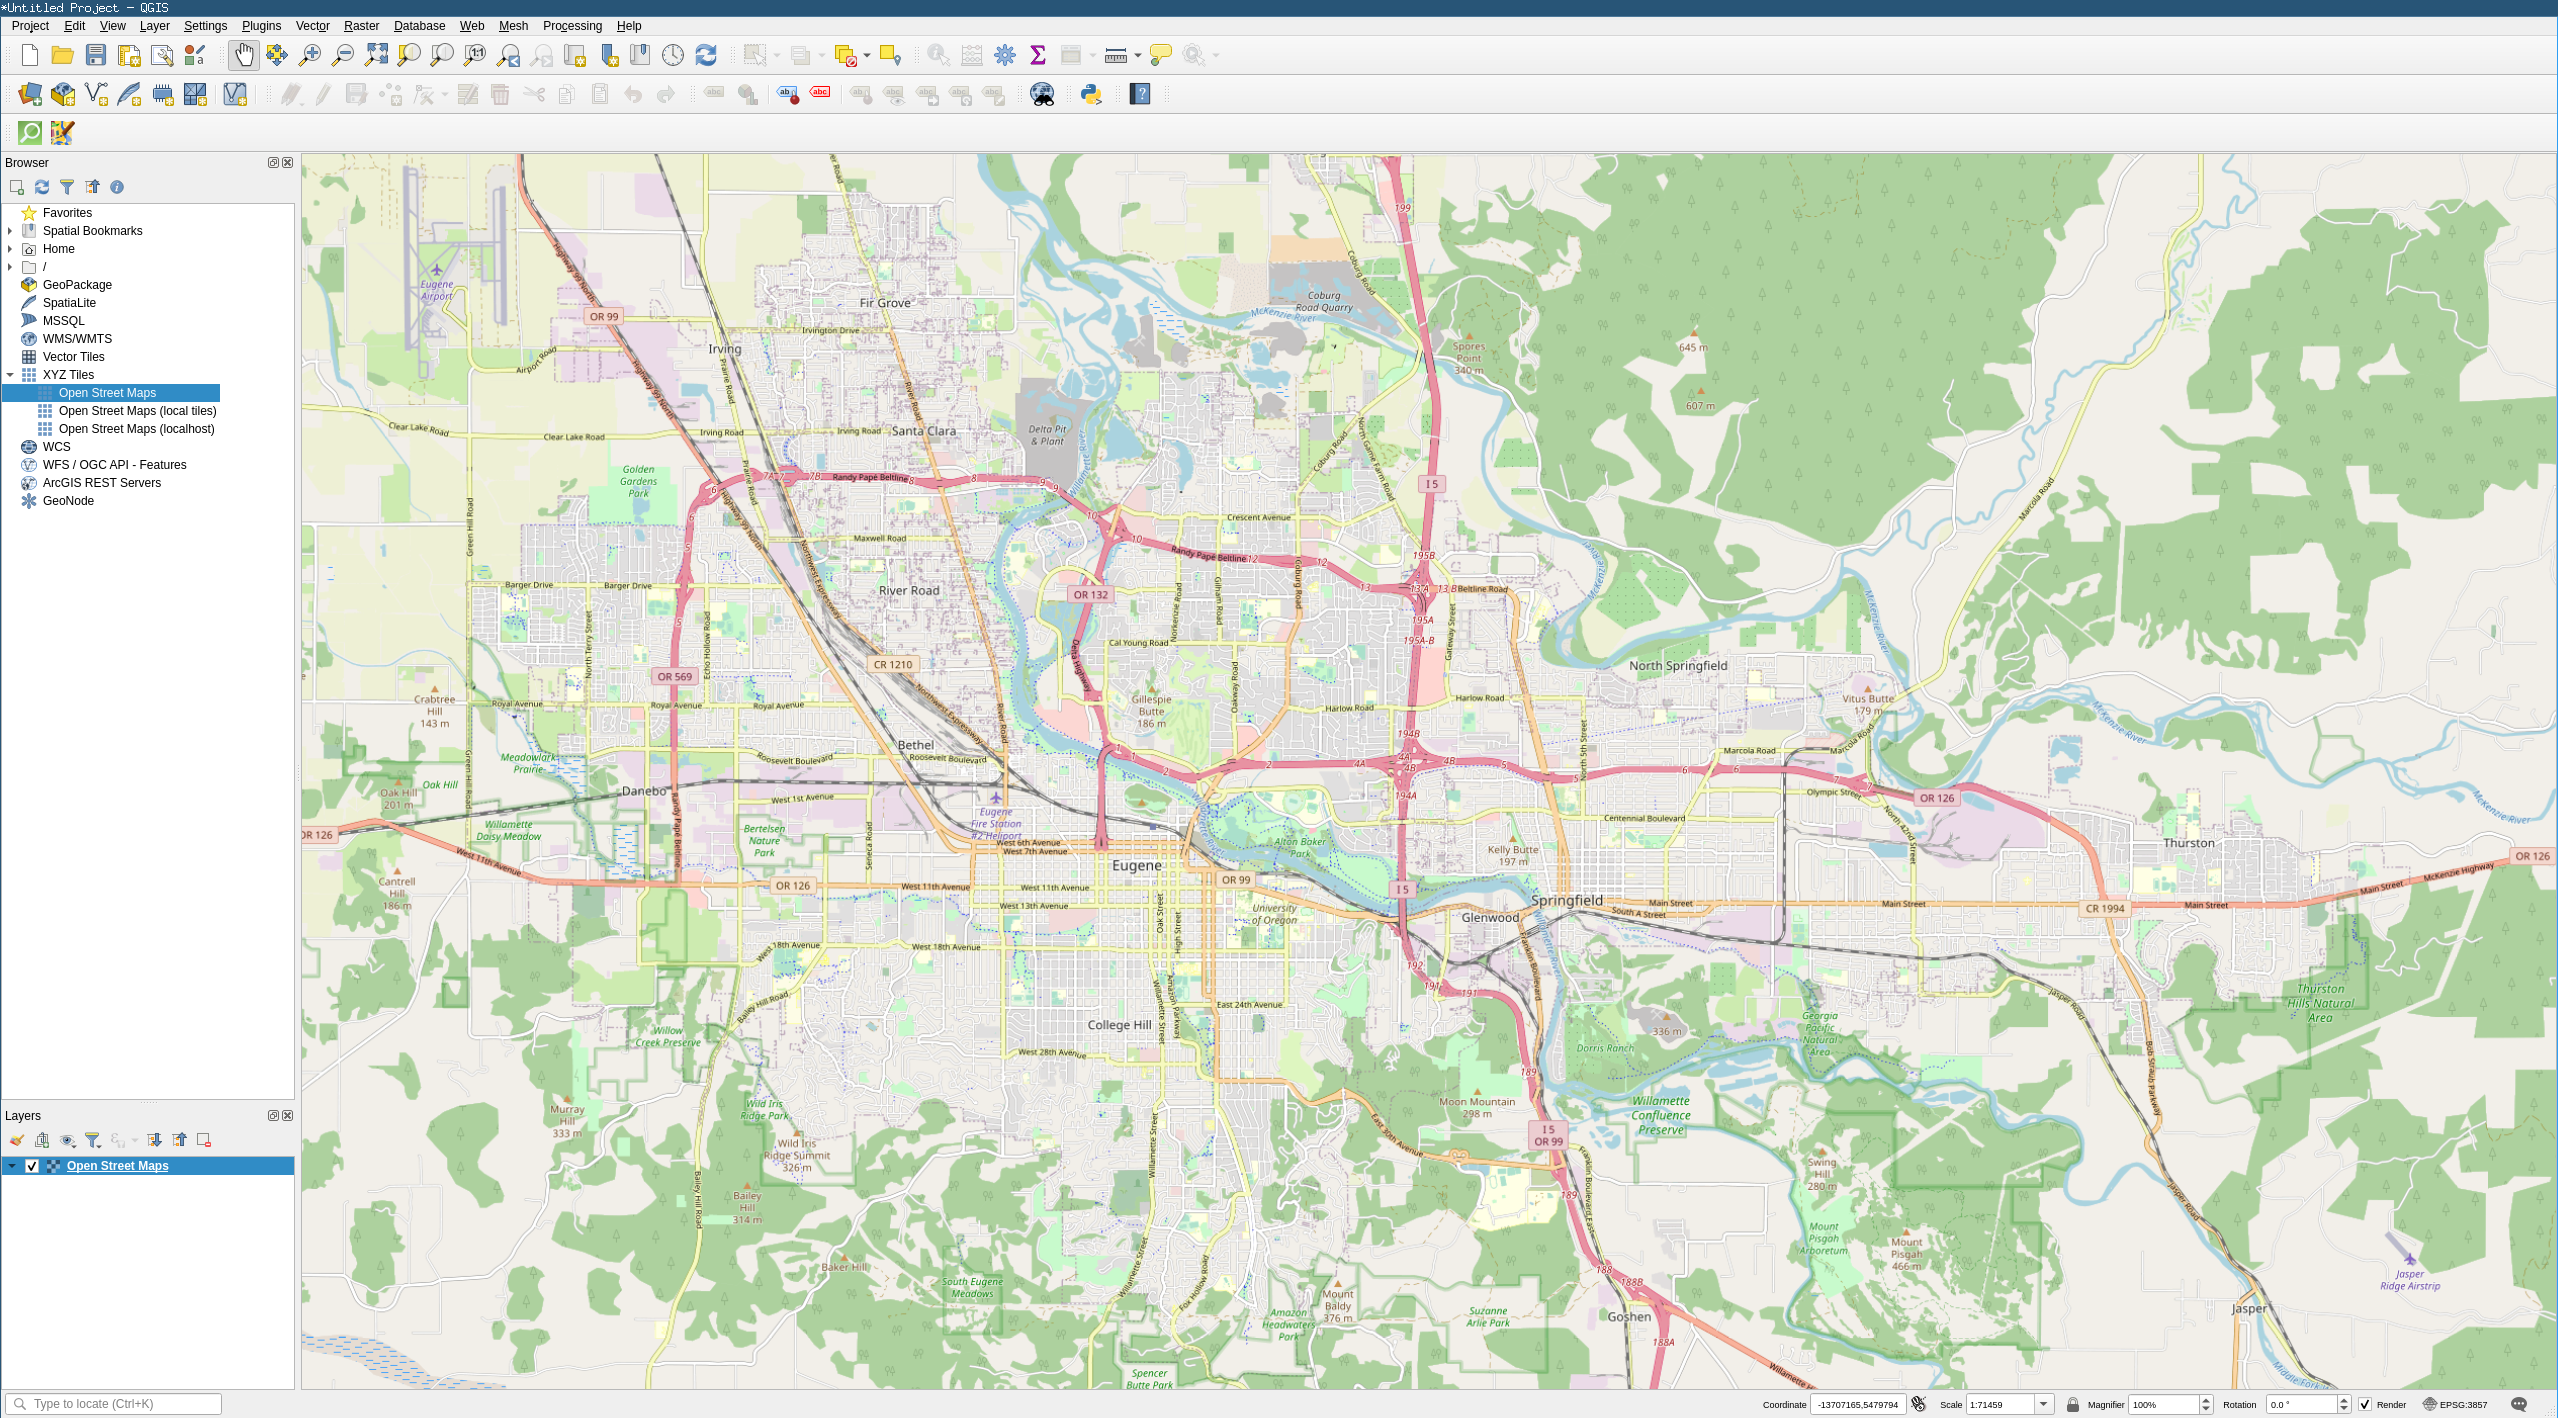
\includegraphics{files/blog/2022_04_17_generating_openstreetmap_tiles_for_offline_slippy_maps/2022_04_17_qgis.png}
\caption{QGIS displaying tiles from the OSM tiles server (see if you can spot the hint that this was taken for this blog after I'd already completed the work).}
\end{figure}

Personally, I think it looks pretty nice and has a surprising amount of detail!  Being reliant on a remote server isn't what I wanted, however, so for the next step I looked into downloading the data for Eugene.

\subsection{Getting the data for Eugene}
It turned out that there were quite a number of ways to \htmladdnormallink{get data}{https://learnosm.org/en/osm-data/getting-data/} from OSM, each catering to specific use cases.  I was not keen to try downloading \htmladdnormallink{the entire planet}{https://wiki.openstreetmap.org/wiki/Planet.osm}, nor was I able to find any extracts for Eugene.  The \htmladdnormallink{main api}{https://wiki.openstreetmap.org/wiki/Downloading_data#For_editing} was meant to be used for editing, while how to use the \htmladdnormallink{Overpass API}{https://wiki.openstreetmap.org/wiki/Overpass_API} was not at all apparent to me, and \htmladdnormallink{the manual}{https://dev.overpass-api.de/overpass-doc/en/} was a bit larger than what I felt like trying to fit into my head at the time.  Eventually I ended up using the "Export" feature on the \htmladdnormallink{main OSM page}{https://www.openstreetmap.org/} which got me a nice 233MB \texttt{.osm} file.  I was able to import the data in QGIS via \texttt{Layer -> Add Layer -> Add Vector Layer}, which led to the following:

\begin{figure}
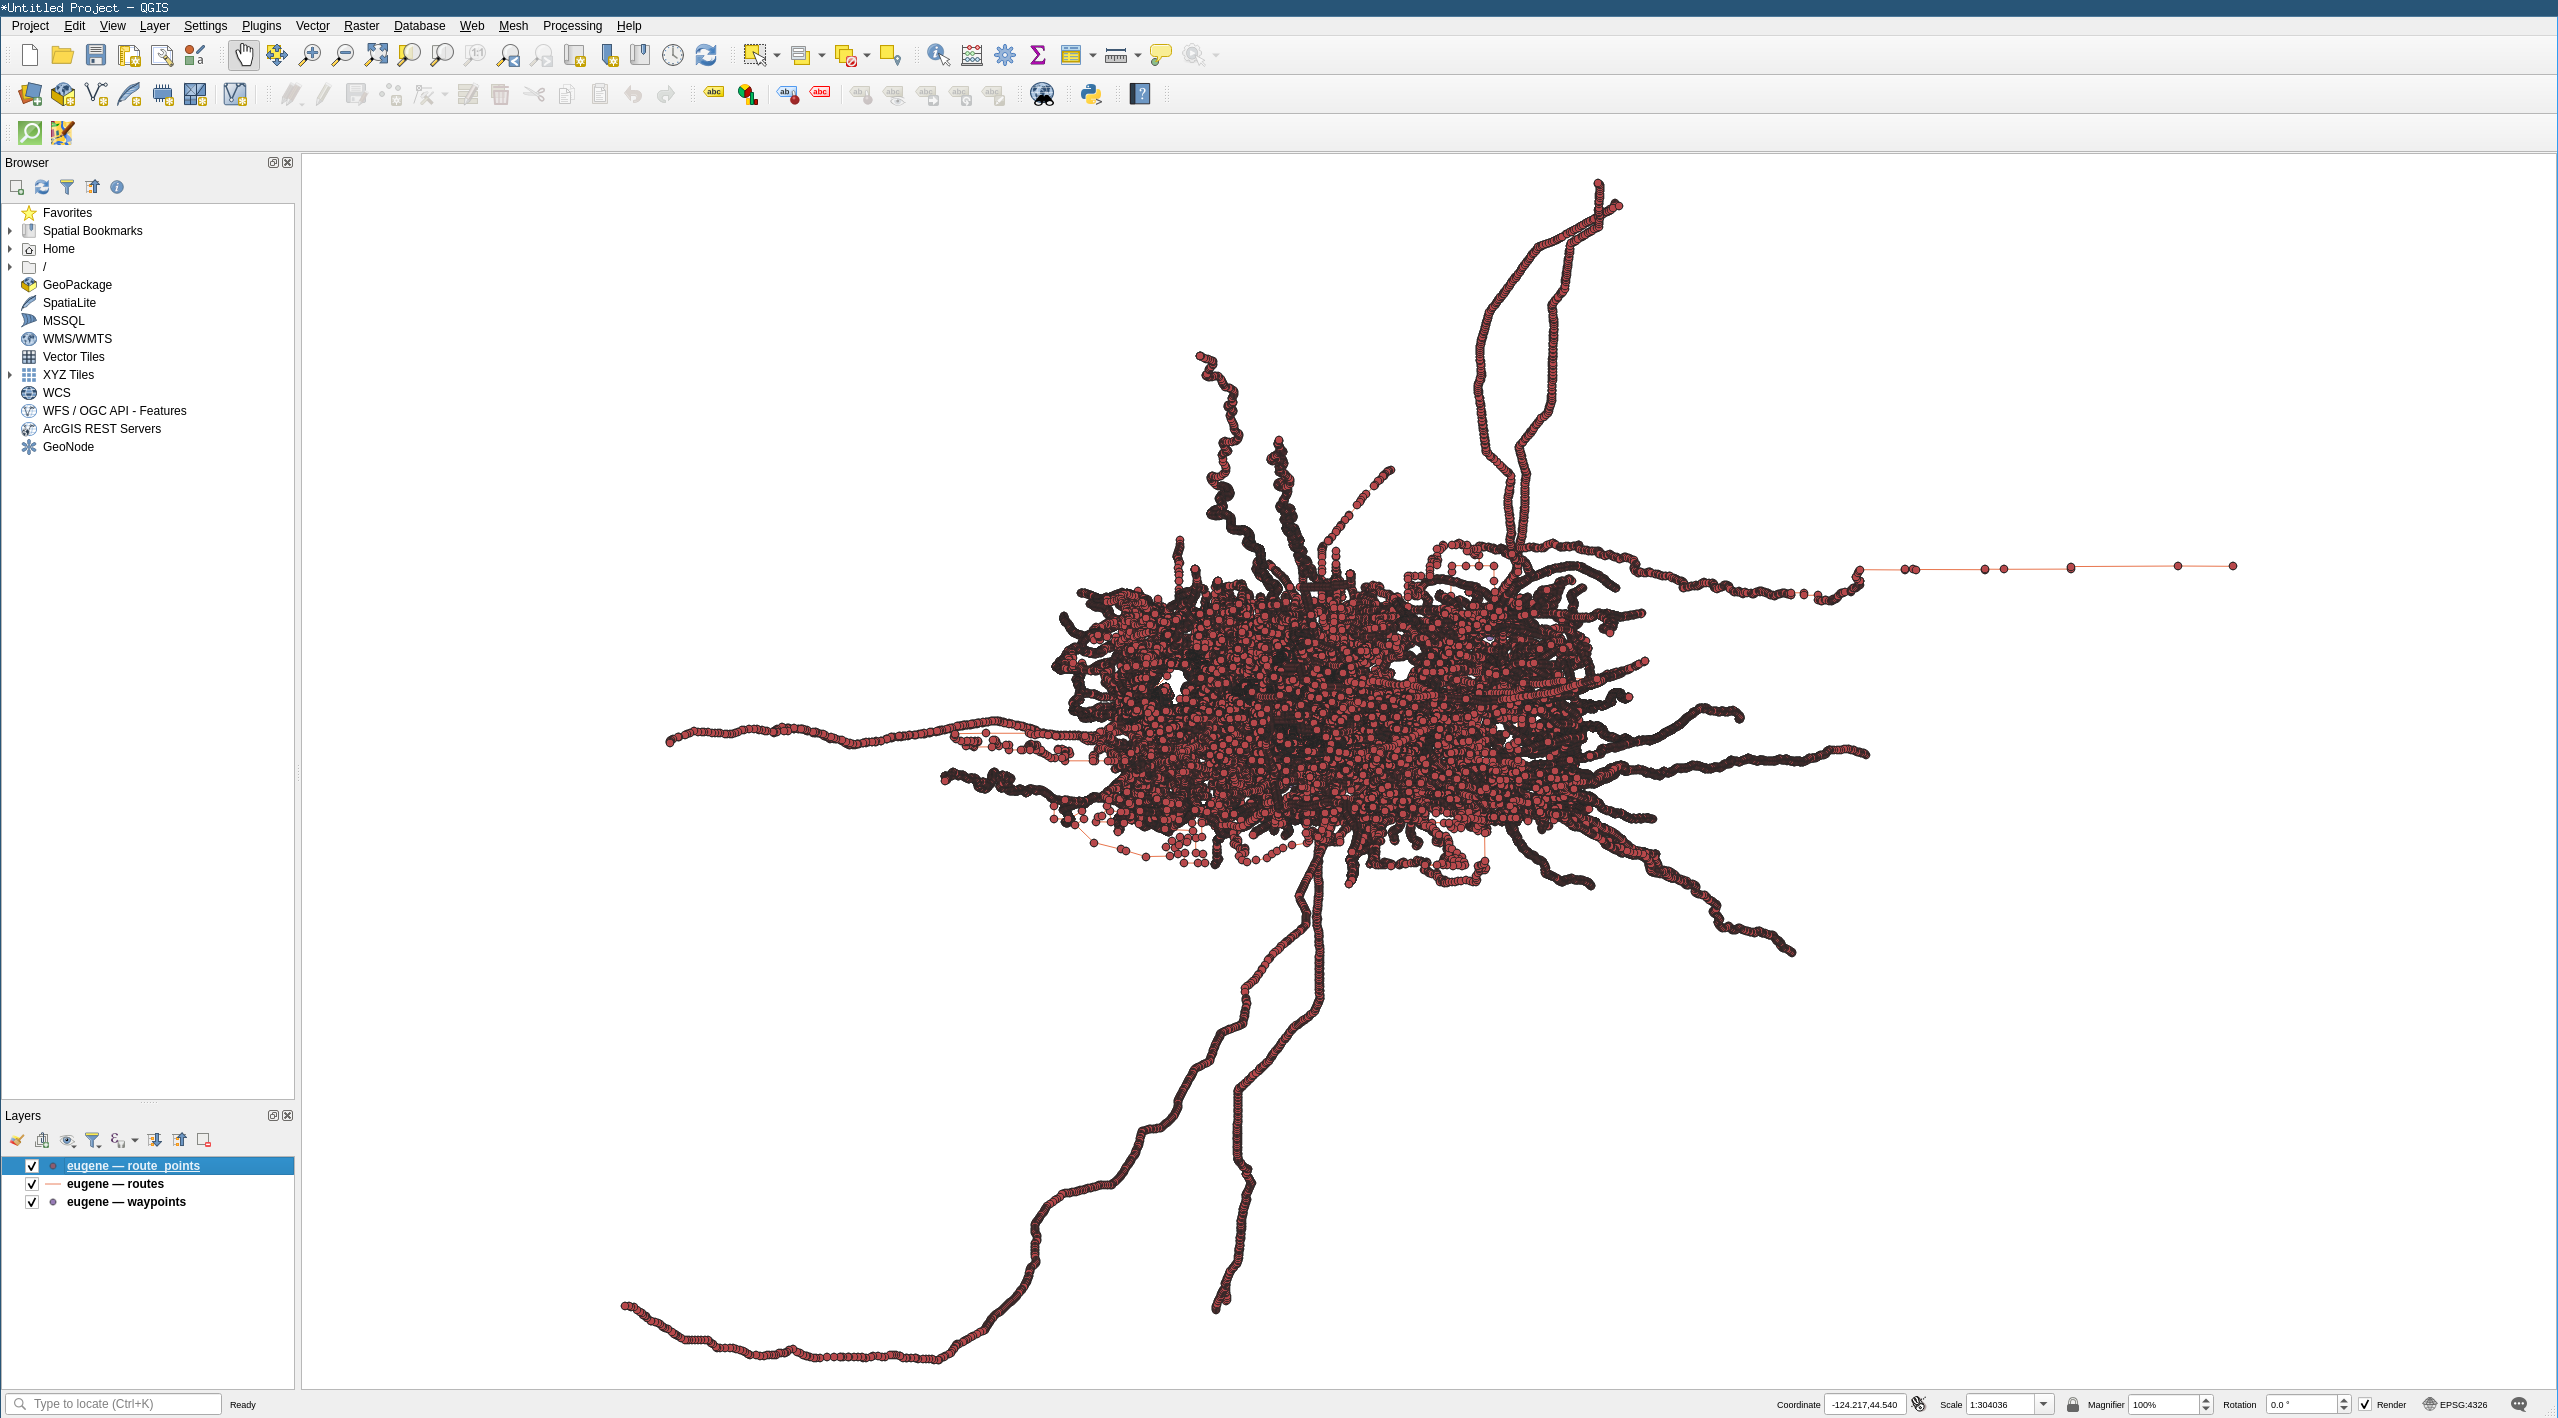
\includegraphics{files/blog/2022_04_17_generating_openstreetmap_tiles_for_offline_slippy_maps/2022_04_17_eugene.png}
\caption{OSM vector data for Eugene.}
\end{figure}

Yikes.  It looks like some kind of lovecraftian horror.  It also liked to crash QGIS, especially if I wasn't extremely gentle with my usage.  What I had thus far wasn't anything close to the nice tiles I was getting from OSM; I needed to figure out how to get those tiles!

\subsection{Turning the data into tiles}
As a quick and hopeful alternative to generating my own tiles I decided to see if I could just fetch the tiles from the OSM map server directly; unfortunately for me, the \htmladdnormallink{policies}{https://operations.osmfoundation.org/policies/tiles/} stated that bulk downloading for high zoom levels was forbidden.  Thus I'd have to take the much more difficult path of rendering my own tiles.  The tool for doing this appeared to be \htmladdnormallink{Mapnik}{https://mapnik.org/}, and it had an unofficial \htmladdnormallink{Gentoo overlay}{https://github.com/redneb/gentoo-mapnik-overlay} which I could use to install it.  How to use this tool directly wasn't obvious to me; I found \htmladdnormallink{this tutorial}{https://github.com/mapnik/mapnik/wiki/GettingStartedInPython} but ran into an error trying to import the module in Python, and it wasn't immediately obvious how I could apply the tutorial towards generating the same kind of tiles used by the OSM server.  Taking this into consideration I decided that the most straightforward method would be to \htmladdnormallink{set up my own tile server}{https://switch2osm.org/serving-tiles/} to see if I could even get tiles consistent with the OSM server.

More precisely, I decided to follow the instructions for a \htmladdnormallink{Debian 11 tile server}{https://switch2osm.org/serving-tiles/manually-building-a-tile-server-debian-11}.  Since I was on Gentoo, the instructions required a number of adaptations (though my notes aren't too good here, I'll document a few problems and their fixes as best I'm able to); I also made reference to \htmladdnormallink{these old Gentoo instructions}{https://wiki.openstreetmap.org/wiki/Deploying_your_own_Slippy_Map_Gentoo#Step_two:_Rendering_toolchain} and \htmladdnormallink{these \texttt{mod_tile} instructions for Ubuntu 20.04}{https://github.com/openstreetmap/mod_tile/blob/master/docs/build/building_on_ubuntu_20_04.md} when necessary.  A few difficulties were encountered when installing the Mapnik Python bindings; first off:

\begin{verbatim}
# ./setup.py install
<snip>
src/mapnik_datasource.cpp:37:10: fatal error: mapnik/geometry/box2d.hpp: No such file or directory
   37 | #include <mapnik/geometry/box2d.hpp>
      |          ^~~~~~~~~~~~~~~~~~~~~~~~~~~
compilation terminated.
error: command '/usr/bin/x86_64-pc-linux-gnu-g++' failed with exit code 1

Missing boost_python boost library, try to add its name with BOOST_PYTHON_LIB environment var.
\end{verbatim}

This was despite having Boost installed with the \texttt{python} \texttt{USE} flag enabled.  So I searched for the installed Python library via \texttt{equery f boost | grep -i python}, found it at \texttt{/usr/lib64/cmake/boost_python-1.77.0}, and re-ran the command:

\begin{verbatim}
# BOOST_PYTHON_LIB=/usr/lib64/cmake/boost_python-1.77.0 ./setup.py install
<snip>
/usr/lib/gcc/x86_64-pc-linux-gnu/11.2.0/../../../../x86_64-pc-linux-gnu/bin/ld: cannot find -l/usr/lib64/libboost_python39.so
collect2: error: ld returned 1 exit status
error: command '/usr/bin/x86_64-pc-linux-gnu-g++' failed with exit code 1
\end{verbatim}

Which then failed at a different point.  Apparently \texttt{BOOST_PYTHON_LIB} expects the soname of the library and not the full path.  Setting \texttt{BOOST_PYTHON_LIB=boost_python39} fixed the issue.

Next, I had some issues getting the ``external data'' when setting up OSM Carto:

\begin{verbatim}
$ ./scripts/get-external-data.py
INFO:root:  Importing into database
CRITICAL:root:ogr2ogr returned 1 with layer simplified_water_polygons
CRITICAL:root:Command line was ogr2ogr -f PostgreSQL -lco GEOMETRY_NAME=way -lco SPATIAL_INDEX=FALSE -lco EXTRACT_SCHEMA_FROM_LAYER_NAME=YES -nln loading.simplified_water_polygons PG:dbname=gis data/simplified_water_polygons/simplified-water-polygons-split-3857/simplified_water_polygons.shp
CRITICAL:root:Output was
<snip>
subprocess.CalledProcessError: Command '['ogr2ogr', '-f', 'PostgreSQL', '-lco', 'GEOMETRY_NAME=way', '-lco', 'SPATIAL_INDEX=FALSE', '-lco', 'EXTRACT_SCHEMA_FROM_LAYER_NAME=YES', '-nln', 'loading.simplified_water_polygons', 'PG:dbname=gis', 'data/simplified_water_polygons/simplified-water-polygons-split-3857/simplified_water_polygons.shp']' returned non-zero exit status 1.

During handling of the above exception, another exception occurred:
<snip>
RuntimeError: ogr2ogr error when loading table simplified_water_polygons
\end{verbatim}

Yikes.  The next step here was to try running the command manually in order to get the actual process output:

\begin{verbatim}
postgres@seneca /home/frostsnow/software/openstreetmap-carto $ ogr2ogr -f PostgreSQL -lco GEOMETRY_NAME=way -lco SPATIAL_INDEX=FALSE -lco EXTRACT_SCHEMA_FROM_LAYER_NAME=YES -nln loading.simplified_water_polygons PG:dbname=gis data/simplified_water_polygons/simplified-water-polygons-split-3857/simplified_water_polygons.shp
ERROR 1: Unable to find driver `PostgreSQL'.
\end{verbatim}

Hmm.  I mapped the program \texttt{ogr2ogr} to its package with \texttt{equery b \$(which ogr2ogr)}, got \texttt{sci-libs/gdal} and noticed that the \texttt{postgres} \texttt{USE} flag was not enabled; enabling it and re-compiling fixed the issue.

Third, I had an issue configuring \texttt{mod_tile}:

\begin{verbatim}
$ ./configure
checking for /opt/local/apache2/bin/apxs... no
configure: error: Could not find apxs on the path.
\end{verbatim}

\ldots because I hadn't installed Apache yet.  D'oh.

That wasn't enough to compile \texttt{mod_tile}, though, as I then ran into the following compilation issue:

\begin{verbatim}
$ make
depbase=`echo src/daemon.o | sed 's|[^/]*$|.deps/&|;s|\.o$||'`;\
gcc -DHAVE_CONFIG_H -I. -I./includes  -pthread -I/usr/include/glib-2.0 -I/usr/lib64/glib-2.0/include    -g -O2 -MT src/daemon.o -MD -MP -MF $depbase.Tpo -c -o src/daemon.o src/daemon.c &&\
mv -f $depbase.Tpo $depbase.Po
src/daemon.c:46:10: fatal error: iniparser/iniparser.h: No such file or directory
   46 | #include <iniparser/iniparser.h>
      |          ^~~~~~~~~~~~~~~~~~~~~~~
compilation terminated.
make: *** [Makefile:887: src/daemon.o] Error 1
\end{verbatim}

Step one was to install \texttt{iniparser}, but I still got the same error.  Turns out that \texttt{iniparser.h} was located in the \texttt{iniparser4} directory, so I had to change \texttt{iniparser/iniparser.h} to \texttt{iniparser4/iniparser.h}.  I got a similar error during linking: \texttt{/usr/lib/gcc/x86_64-pc-linux-gnu/11.2.0/../../../../x86_64-pc-linux-gnu/bin/ld: cannot find -liniparser} which was solved by editing \texttt{Makefile} to use \texttt{-liniparser4}.  Hardly a proper fix, but effective enough to move on.

Then I had trouble starting Apache:

\begin{verbatim}
# rc-service apache2 restart
 * apache2 has detected an error in your setup:
AH00526: Syntax error on line 7 of /etc/apache2/modules.d/11_mod_tile.conf:
Invalid command 'ModTileTileDir', perhaps misspelled or defined by a module not included in the server configuration
\end{verbatim}

The solution here was to explicitly load the tile module via opening \texttt{/etc/apache2/httpd.conf} and adding the line \texttt{LoadModule tile_module modules/mod_tile.so}.

Even though I had Apache running at this point, I wasn't able to view any tiles.  I found the source of the problem by opening \texttt{/var/log/apache2/error_log} and finding the following log message:

\begin{verbatim}
[Sat Jan 29 18:12:49.629646 2022] [tile:warn] [pid 22362] [client 127.0.0.1:38558] socket connect failed for: /run/renderd/renderd.sock with reason: No such file or directory
[Sat Jan 29 18:12:49.629675 2022] [tile:notice] [pid 22362] [client 127.0.0.1:38558] Failed to connect to renderer
\end{verbatim}

The easiest workaround (and bad; don't try this at home) was to set \texttt{chmod 0777} on the file; this worked, and I made a note to fix it later.

Eventually I got everything set-up and tried out the sample leaflet.  At first I saw the outlines of all the continents and was worried that somehow external data was being pulled in, but then I remembered that some extra data was pulled in magically by one of OSM's scripts earlier.  As I zoomed into Oregon, I saw it:

\begin{figure}

\includegraphics{files/blog/2022_04_17_generating_openstreetmap_tiles_for_offline_slippy_maps/2022_04_17_working.png}
\caption{OSM tiles locally-rendered and served via the sample leaflet.}
\end{figure}

Hurrah!  For convenience's sake I then wrote a few OpenRC scripts so that I didn't have to manually invoke Apache, PostgreSQL, and \texttt{renderd}; \texttt{/etc/init.d/renderd}:

\begin{verbatim}
#!/sbin/openrc-run
# Copyright 2022 Gentoo Authors
# Distributed under the terms of the GNU General Public License v2

name="renderd daemon"
description=""
command=/usr/local/bin/renderd
command_args="${renderd_args}"
command_user=postgres:postgres

depend() {
        need apache2 postgresql-13
}

start_pre() {
        checkpath -d --owner root:postgres --mode 0775 /run/renderd
}
\end{verbatim}

and \texttt{/etc/conf.d/renderd}:

\begin{verbatim}
# /etc/conf.d/minetest-server: config file for /etc/init.d/minetest-server

# pidfile
PIDFILE="/run/renderd/renderd.pid"
\end{verbatim}

Yes, I used the \texttt{postgres} user for anything involving \texttt{renderd}.  A proper set up would decouple the two, but \texttt{renderd} was the only thing using PostgreSQL so it didn't seem like a big deal and I didn't want to bother creating another user.

As for QGIS, pulling from the local webserver was simple enough: create a new \texttt{XYZ tiles} layer and set it's \texttt{Layer Source} URL to \verb|http://127.0.0.1/hot/{z}/{x}/{y}.png|.  Although (sadly) a little slower than pulling from OSM's server, it worked!

\subsection{Pulling tiles from the webserver}
Though I now had the tiles being served from a local webserver, my goal was to have tiles without having to run a webserver at all.  Looking at \texttt{renderd}'s offerings, the \texttt{render_list} command seemed like it might be useful for the task.  Before I could invoke the command, I needed the tile co-ordinates.  Mapping x and y values was explained in the \htmladdnormallink{slippy map tilenames}{https://wiki.openstreetmap.org/wiki/Slippy_map_tilenames} Wiki page, except the formula expected degrees and QGIS was displaying something else; I was able to get QGIS to display degrees by going to \texttt{Project -> Properties}, \texttt{General} tab, \texttt{Coordinate and Bearing Display} subsection, then changing the \texttt{Display coordinates using} drop-down from \texttt{Map units (meters)} to \texttt{Decimal Degrees}.  At that point the widget on the bottom reading \texttt{Coordinate} displayed only coordinates for my mouse; clicking the icon next to it changed the widget to display \texttt{Extents} instead.  This gave me co-ordinates -123.2519,43.9809:-122.8547,44.1422 for an extent covering Eugene.  As for the zoom levels, I'm still perplexed as to how QGIS's \texttt{Scale} corresponds to the \htmladdnormallink{zoom levels}{https://wiki.openstreetmap.org/wiki/Zoom_levels} Wiki page's "Scale", given that QGIS displayed 1:128807296 for the world while the Wiki page claimed 1:500000000.  My easy workaround for finding the required minimum required zoom level was to clean the tiles cache, navigate to the desired extent, then run \texttt{ls /var/lib/mod_tile/s2o} and see which zoom levels were used (actually, in retrospective, it makes sense to generate tiles for the lower zoom levels so one can see the general area one needs to zoom in on).  X, y, and z values in hand I used the Python formula, shamelessly copy \& pasted from the OSM Wiki, to get the tile co-ordinates I needed:

\begin{verbatim}
import math
def deg2num(lat_deg, lon_deg, zoom):
  lat_rad = math.radians(lat_deg)
  n = 2.0 ** zoom
  xtile = int((lon_deg + 180.0) / 360.0 * n)
  ytile = int((1.0 - math.asinh(math.tan(lat_rad)) / math.pi) / 2.0 * n)
  return (xtile, ytile)
\end{verbatim}

Though \texttt{renderd_list} wasn't co-operating when I invoked it:

\begin{verbatim}
** (process:10517): ERROR **: 19:04:08.262: init_storage_backend: No valid storage backend found for options: s2o/
Failed to initialise storage backend s2o/
\end{verbatim}

It turned out that I needed to pass the tile cache directly via \texttt{-t /var/lib/mod_tile}.  The program then ran, but did nothing.  Argh!  Eventually I searched \texttt{/var/log/messages} and found the following:

\begin{verbatim}
Feb 12 19:06:01 seneca renderd[2618]: ERROR: No map for: default
\end{verbatim}

The fix here was to explicitly tell the program to use the \texttt{s2o} map via \texttt{-m s2o}.  Now the tiles were rendering!

Unfortunately for me, the \texttt{renderd} tiles were stored on-disk in a \htmladdnormallink{special layout}{https://github.com/openstreetmap/mod_tile#details-about-mod_tile-tile-serving} that was mapped to the appropriate pages by the Apache module but was not suitable for direct file access!  Some digging in the source showed a man page for a \texttt{convert_meta} utility, though it was not installed on my system.  This utility appeared to have been written primarily to convert from a ``plain'' format (which I wanted) to \texttt{renderd}'s special format; it also appeared to be able to convert from the special format back to a plain format.  I tried my hand at enabling and compiling this utility but was not at all successful; it seems to have long been bit-rotted.  Instead, I ended up writing a dumb script to pull all the tiles I needed:

\begin{verbatim}
#!/bin/bash

# No nested arrays in bash, so manually ensure these line-up.
# Eugene.
zooms=(11 12 13 14 15 16 17 18)
xmins=(322 645 1291 2582 5165 10331 20663 41327)
xmaxs=(325 650 1300 2601 5202 10404 20809 41618)
ymins=(743 1487 2974 5948 11897 23794 47589 95178)
ymaxs=(744 1489 2979 5958 11917 23835 47671 95343)
dest="media/tiles"

set -x
mkdir -p "${dest}"
pushd "${dest}"
for (( i=0 ; i<${#zooms[@]} ; i++ )); do
        zoom=${zooms[$i]}
        xmin=${xmins[$i]}
        xmax=${xmaxs[$i]}
        ymin=${ymins[$i]}
        ymax=${ymaxs[$i]}

        # Render tiles.
        #render_list -z ${zoom} -Z ${zoom} -a -x ${xmin} -X ${xmax} -y ${ymin} -Y ${ymax} -t /var/lib/mod_tile -f -m s2o

        # Pull tiles.
        mkdir -p "${zoom}"
        pushd "${zoom}"
        for (( x=${xmin} ; x<=${xmax} ; x++ )); do
                mkdir -p "${x}"
                pushd "${x}"
                for (( y=${ymin} ; y<=${ymax} ; y++ )); do
                        wget -c "http://localhost/hot/${zoom}/${x}/${y}.png"
                done
                popd
        done
        popd
done
set +x
\end{verbatim}

As I said, it's pretty dumb: a real script would do something like accept an extent and then dynamically calculate the co-ordinates, but I didn't feel like figuring out all the trigonometry in \texttt{bash}, \texttt{bc}, or calling out to an inline Python script.  It also probably doesn't need the \texttt{render_list} call since the webserver will just dynamically generate any missing tiles.  There's also probably a sane way to make multiple calls to \texttt{wget} so it doesn't send a bajillion separate connections.  Anyways, awfulness aside, the script did work to pull all of the tiles over about 5-10 minutes!  The data took up about 366MB; a very reasonable amount!

\ldots but would QGIS be able to use the local tiles?  While the \texttt{Layer Source}'s \texttt{URL} parameter \emph{should} accept a perfectly valid \texttt{file://} URL, that didn't mean that it'd actually work.  I was able to save the layer, but when I opened it again and double-checked its properties the URL entry was blank!  I entered and saved it again, and got the same result!  Yet, when I actually tried navigating in the map, it worked!  It was \emph{fast}, too.  So, apparently the user interface didn't understand the URL, but the underlying library sure appeared to.

Local tiles for Eugene in hand, I had the cornerstone of what I was looking for and a basis to build upon.  The tiles were currently limited to Eugene, and I decided it'd be nice to have tiles for all of Oregon in case I needed to travel somewhere in-state.

\subsection{Tiles for all of Oregon}
First step to generating tiles for all of Oregon was to find a way to get the needed data.  Since \htmladdnormallink{planet.osm}{https://wiki.openstreetmap.org/wiki/Planet.osm} was some tens to hundreds of gigabytes (depending on compression level), I decided to find a way to get a more specific subset of the data.  At first I tried to use the \htmladdnormallink{QuickOSM}{https://github.com/3liz/QuickOSM} plugin, but no plugins were installable; I had to first re-compile QGIS with the \texttt{python} \texttt{USE} flag.  After I'd gotten the plugin installed, I tried to get all of the data for Oregon but a large query would timeout while a smaller query spewed the error \texttt{Error on the layer : points is not valid}.  Judging from the \htmladdnormallink{Overpass API Limitations}{https://wiki.openstreetmap.org/wiki/Overpass_API#Limitations}, my best guess was that Oregon was just to big to get data from; the limitations entry also suggested using existing static extracts, but I wasn't sure if I'd be able to find one.

One of the entries on the Learn OSM \htmladdnormallink{getting data}{https://learnosm.org/en/osm-data/getting-data/} page listed \htmladdnormallink{GeoFabrik extracts}{https://download.geofabrik.de/}.  All of \htmladdnormallink{North America}{https://download.geofabrik.de/north-america.html} was available at 11.3GB.  Drilling down, I found \htmladdnormallink{US Pacific}{https://download.geofabrik.de/north-america/us-pacific.html}, er, but that was only 129MB while what I'd downloaded for Eugene earlier was 233MB; perhaps this was just Hawaii or something and not the U.S. Pacific timezone area?  \htmladdnormallink{US West}{https://download.geofabrik.de/north-america/us-west.html} seemed then a more likely candidate, but I could do without California and Washington (and not just in a data sense).  Thankfully, ignoring the ``Special Sub Regions'' section and instead looking at the ``Sub Regions'' section and choosing the \htmladdnormallink{United States of America}{https://download.geofabrik.de/north-america/us.html} had its own special \htmladdnormallink{Oregon}{https://download.geofabrik.de/north-america/us/oregon.html} sub-region at 178MB (presumably smaller than Eugene's 233MB because Eugene's \htmladdnormallink{file format}{https://learnosm.org/en/osm-data/file-formats/} was OSM while this was OSM PBF), perfect!  A quick download and database update later it was then time to begin tile-generation.

The basics of generating tiles were pretty much the same as with Eugene, except I used the approximate extent for Oregon -126.2197,41.9052:-114.9559,46.3326 and a max zoom level of 7:

\begin{verbatim}
zooms=(7 8 9 10 11 12 13 14 15 16 17 18)
xmins=(19 38 76 152 305 611 1223 2447 4895 9790 19580 39161)
xmaxs=(23 46 92 185 370 740 1480 2960 5920 11840 23681 47363)
ymins=(45 90 181 362 725 1451 2903 5806 11613 23227 46455 92911)
ymaxs=(47 95 190 380 760 1521 3043 6087 12175 24351 48702 97405)
\end{verbatim}

The first thing I noticed was that generating this set of tiles was taking much longer.  By which I mean that generating Eugene's tiles seemed to take a little over 5 minutes while Oregon's took about a \emph{week}.  The amount of generated data was huge: 198G of raw tiles and 35G in \texttt{renderd}'s cache (note: the latter may be an underestimate as the large amount of data generated may have triggered auto-cleaning mechanisms in \texttt{renderd}).  Well, that's not exactly what I'd call \emph{practical}.  Pre-generating tiles for a city is thus feasible, but at the state level one would want to dynamically generate tiles or use some kind of heuristic to only generate tiles for their target areas.

\subsection{Conclusion}
Thus I was able to generate my own OSM tiles with some moderate effort using current infrastructure.  QGIS was flexible enough to use either the OSM tile server, a localhost tile server, or even a filepath to tiles on the filesystem (though the configuration UI did appear to be a bit confused by this one).  Setting up a webserver took some effort, but the solid documentation on the LearnOSM website proved to be a good foundation for the task.  Pre-generated city tiles were small enough to easily fit on all systems except, perhaps, embedded systems, but state tiles were too big for all but desktops or servers.  With local tiles on disk I no longer needed to worry about that one aspect of surveillance capitalism.  Perhaps the next step would be to look into routing solutions, since addresses are not clear from tiles and tracing routes by hand is mildly laborious.  For now, time to sit back and admire my beautiful tiles.


% Removing Extra IP Protocols
\section{2022-04-03 Removing Extra IP Protocols}
Back when I was a fledgeling programmer, I took a trip to a nearby book store hoping to learn some l33t sk711z.  There I found a copy of ``\htmladdnormallink{Nmap Network Scanning}{https://nmap.org/book/}'' by Gordon ``Fyodor'' Lyon and it sounded pretty l33t, so I bought a copy and then began to read it.  One piece of knowledge I got from reading the book is that besides the usual TCP and UDP scans, \texttt{nmap} also has an IP Protocol scan, which scans for, well, IP protocols, rather than TCP or UDP ports.  The scan was quick and painless for me to run, but how to interpret the results and then remove the unneeded protocols was not apparent to me.  Over a decade after reading the book, I decided to take a serious look at analyzing and removing unused IP protocols from my network.

First step was to amalgamate all of the not-closed protocols into a list, since the methods for eliminating a protocol would be the same across the various systems (though not so much as I had hoped, as will be explained below):

\begin{verbatim}
1        open          icmp
2        open|filtered igmp
4        open|filtered ipv4
6        open          tcp
17       open          udp
41       open|filtered ipv6
47       open|filtered gre
69       open|filtered sat-mon
90       open|filtered sprite-rpc
102      open|filtered pnni
103      open|filtered pim
136      open|filtered udplite
255      open|filtered unknown
\end{verbatim}

The necessary protocols which I was familiar with are \htmladdnormallink{ICMP}{https://en.wikipedia.org/wiki/Internet_Control_Message_Protocol} (ping, \&c.), \htmladdnormallink{TCP}{https://en.wikipedia.org/wiki/Transmission_Control_Protocol}, and \htmladdnormallink{UDP}{https://en.wikipedia.org/wiki/User_Datagram_Protocol}.  The rest would require investigation.

\subsection{\texttt{igmp} and \texttt{pim}}
First on the list was \htmladdnormallink{\texttt{igmp}}{https://en.wikipedia.org/wiki/Igmp}.  Judging from the Wikipedia page, this protocol is useful for streaming large amounts of data (such as video) to numerous clients and is part of \htmladdnormallink{IP multicast}{https://en.wikipedia.org/wiki/IP_multicast}.  Well, I was pretty sure I didn't do anything like that, so I decided to axe it and see if anything broke!  Some searching through the Linux kernel config turned up a \texttt{CONFIG_IP_MULTICAST} option; I disabled this, recompilled and installed the new kernel, and then both \texttt{IGMP} \emph{and} \htmladdnormallink{\texttt{PIM}}{https://en.wikipedia.org/wiki/Protocol_Independent_Multicast} were now closed!  Things were off to an excellent start.

\subsection{\texttt{sat-mon}, \texttt{sprite-rpc}, and \texttt{pnni}}
When I attempted to re-verify that the \texttt{sat-mon} protocol was still open/filtered before trying to close it, I found that the filter was now reported as closed!  Though I know that \texttt{nmap} has built-in ratelimiting, perhaps that wasn't enough to avoid all false positives?  I applied the same workaround which I wrote about in a previous blurb, that is, setting \texttt{/proc/sys/net/ipv4/icmp_ratemask} to \texttt{6160} and \texttt{/proc/sys/net/ipv4/icmp_msgs_per_sec} to \texttt{1000000}.  A few, now very fast, rescans showed that not only the \texttt{sat-mon}, but also the \texttt{sprite-rpc} and \texttt{pnni} protocols were now reported as closed!

\subsection{\texttt{ipv4} and \texttt{ipv6}}
Turns out I had forgotten to disable IPv6 on one of my machines (I can already sense IPv6 advocates frothing at the mouth)!  Unsetting \texttt{CONFIG_IPV6}, re-compiling, and re-installing the kernel as well as globally disabling the \texttt{ipv6} USE flag and re-building \texttt{@world} (it's a \htmladdnormallink{Gentoo}{https://www.gentoo.org/} thing) made both protocols report as closed.  What's odd about this is that all my machines use IPv4 and the scans themselves took place over IPv4, but the protocol was marked as closed on them; even on my router, which supports both IPv4 an IPv6, both protocols were reported as closed.  Well, whatever, it's good enough as-is.

\subsection{\texttt{udplite}}
This one was tricky.  Apparently the purpose of \htmladdnormallink{UDP-Lite}{https://www.kernel.org/doc/html/latest/networking/udplite.html} is to allow programs with built-in error-recovery to handle broken packets rather than discard them because the regular UDP checksum failed.  Makes sense, but do any programs that I run actually use this?  Should I be scanning all 65536 UDP-Lite ports as well, or can I just axe the protocol?  Well, the fun way to find out is to axe it and see if anything breaks.  Unfortunately, this was not so straightforward.  I found nothing akin to a config option to disable the protocol from searching the kernel's \texttt{menuconfig}, nor did I find anything obvious when digging through the kernel source file \texttt{net/ipv4/udplite.c}.  Patching and then remembering to patch each kernel as part of the upgrade process was not something that I was particularly keen on doing, either; instead, I decided to try using \texttt{iptables}.

First step was to enable both \texttt{CONFIG_IP_NF_IPTABLES} and \texttt{CONFIG_IP_NF_TARGET_REJECT} in the kernel (then recompile, reinstall, \&c.).  Next step was to disable the protocol with \texttt{iptables -A INPUT -p udplite -j REJECT}, but a subsequent rescan now showed the protocol as \texttt{open}!  Reading the \texttt{iptables-extensions(8)} manpage revealed that the default error message sent by the IPv4 \texttt{REJECT} target is \texttt{icmp-port-unreachable}; this would explain why the \emph{protocol} itself was reported as open: the rejection is only sent when trying to connect to a specific \emph{port} within the protocol.  Further reading showed that issue could be remedied by adding the \texttt{\verb|--|\texttt{reject-with icmp-proto-unreachable}} option to the command, giving \texttt{iptables -A INPUT -p udplite -j REJECT \verb|--|reject-with icmp-proto-unreachable}.  Running this gave the desired result of \texttt{closed}, but, since this was not a hard-disable at the kernel level, a few additional steps had to be taken to persist this change.  On Gentoo, the following series of commands did the trick: \texttt{rc-service iptables save}, \texttt{rc-service iptables start}, and \texttt{rc-update add iptables default}; simple enough!  For my LibreCMC router, I added the aforementioned \texttt{iptables} command to the file \texttt{/etc/firewall.user}.  A reboot and rescan on the respective machines showed that these steps gave the desired result.

There remains the fundamental question of whether or not the additional complexity involved in disabling the protocol outweighs the benefits from disabling the protocol; perhaps it would have been better to come up with a method for patching the kernel and thus removing the additional netfilter complexity from the non-router systems.  Perhaps, but netfilter is what I used this time around.

\subsection{\texttt{igmp} \& LibreCMC}
The reality of computing is that not all computers are created equal.  What this meant for me in this case was that, while I certainly knew how to configure and update kernels on my regular Gentoo installs, I was not certain how to do so on LibreCMC.  I'd previously downloaded and compiled LibreCMC, but when I looked through \texttt{make menuconfig} I did not find any relevant options; turns out I needed to run \texttt{make kernel_menuconfig} instead.  I did the first step of disabling \texttt{CONFIG_IP_MULTICAST}, then, for good measure, I decided to disable \texttt{CONFIG_IPV6} as well.  After rebuilding and flashing the image the "SYS" light blinked as normal, then began blinking rapidly\ldots~forever.  Okay, well, I did the usual method of holding down the reset button for 30 seconds in order to trigger a factory reset.  Nothing happened.  Fuck.  It was about 7:30 p.m. on a Sunday, and I wanted the router working before starting the workweek given that I was working from home.

My first inclination was to try opening the router in order to see if I could flash it.  While the top of the router looked easily removable, there was some kind of unexpected resistance near the back of the router which I hadn't been able to figure out on previous attempts.  Turns out the trick was to remove the\ldots~friction dohickies on the bottom the router, exposing screws which kept the top in place:

\begin{figure}
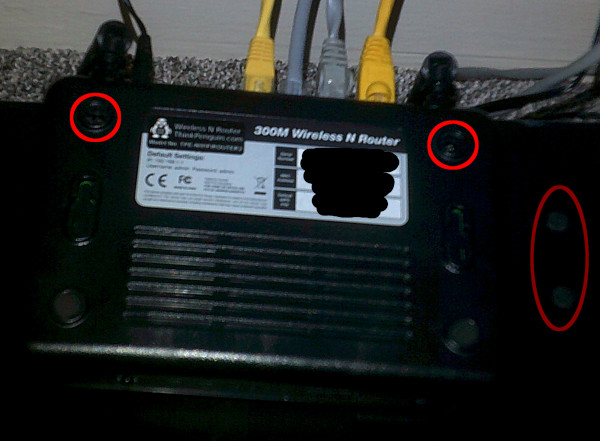
\includegraphics{files/blog/2022_04_03_removing_extra_ip_protocols/2022_04_03_router1.jpg}
\caption{My router with the friction dohickies removed and placed on the side.  There are screws showing which are not really discernable due to my awful camera.}
\end{figure}

With the board exposed, I tried searching for an obvious serial connection, though nothing definite stuck out at me.  Some searching turned up \htmladdnormallink{this page}{https://openwrt.org/toh/tp-link/tl-wr841nd#serial_console} and, more specifically, \htmladdnormallink{this board configuration}{https://openwrt.org/_detail/media/tplink/tl-wr841/tl-wr841nd-v8.4_serial_02.jpg?id=toh\%3Atp-link\%3Atl-wr841nd}, although none of them quite matched my board:

\begin{figure}
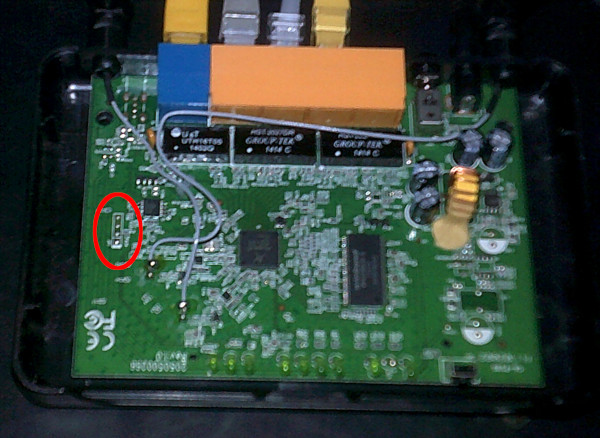
\includegraphics{files/blog/2022_04_03_removing_extra_ip_protocols/2022_04_03_router2.jpg}
\caption{Judging from the similar boards, I'm guessing the circled area is the serial connection.}
\end{figure}

At this point a multitude of problems struck me.  First, the board required a certain type of serial connector.  I thought I ordered one when I got the board, but I couldn't find it, so perhaps I was mis-remembering.  Next, I had no knowledge of how to determine the exact pinout besides extrapolating from the other images of pinouts, a risky bet, and I quite probably did not even have the required equipment.  Last, I'd have to solder the pins in order to connect them, which would add extra difficulty to the task.  Since there was still some kind of life in the board, I decided to see if there was some other way to fix it.

There were two known states which I was able to put the board in.  The first, as mentioned before, was to simply power on the board, which would cause the "PWR" light to turn on and the "SYS" light to flash, then begin flashing "rapidly" ad infinitum.  The second state was obtained by holding down the "WPS/Reset" button during power on; this would cause the "PWR" light to turn on and then all lights to flash about once a second for around 15 seconds before leaving just the "PWR" light on.  Yet I had no idea what either of these statuses meant, nor how to take advantage of them.  A \htmladdnormallink{number}{https://openwrt.org/toh/tp-link/tl-wr841nd#tftp_recovery_via_bootloader_for_v8_v9_v10_v11_v12_v13} \htmladdnormallink{of}{https://community.tp-link.com/en/home/forum/topic/81462?page=1} \htmladdnormallink{pages}{https://forum.archive.openwrt.org/viewtopic.php?id=33906} mentioned the router could pull images from TFTP while in some kind of \htmladdnormallink{failsafe}{https://openwrt.org/docs/guide-user/troubleshooting/failsafe_and_factory_reset#failsafe_mode} mode.  In order to see if this method was viable, I followed the advice of trying to listen for a TFTP request by setting up a static IP address on another machine and then monitoring network traffic with \texttt{tcpdump -Ani enp5s4}; what I found was that the second state (holding down the "WPS/Reset" button during power on) would generate the following traffic when the lights would stop blinking:

\begin{verbatim}
--------
22:52:54.119282 ARP, Request who-has 192.168.1.2 tell 192.168.1.1, length 46
........df...*................................
22:52:54.119327 ARP, Reply 192.168.1.2 is-at 00:14:d1:24:88:f0, length 28
...........$......df...*....
22:52:54.119368 IP 192.168.1.1.6666 > 192.168.1.2.6666: UDP, length 29
E..9..@...._.........
.
.%..U-Boot 1.1.4  (Jul 28 2014)


22:52:54.119399 IP 192.168.1.2 > 192.168.1.1: ICMP 192.168.1.2 udp port 6666 unreachable, length 65
E..UJ...@...................E..9..@...._.........
.
.%..U-Boot 1.1.4  (Jul 28 2014)


22:52:54.119453 IP 192.168.1.1.6666 > 192.168.1.2.6666: UDP, length 7
E..#..@....t.........
.
....uboot> ...........
22:52:54.119465 IP 192.168.1.2 > 192.168.1.1: ICMP 192.168.1.2 udp port 6666 unreachable, length 43
E..?J...@..$..........O.....E..#..@....t.........
.
....uboot>
22:52:59.149647 ARP, Request who-has 192.168.1.1 tell 192.168.1.2, length 28
...........$................
22:52:59.149748 ARP, Reply 192.168.1.1 is-at 64:66:b3:9d:17:2a, length 46
........df...*.......$........................
--------
\end{verbatim}

This looks to be some kind of U-boot CLI prompt, but to port 6666?  Over UDP?  Huh?!  Other pages mentioned emergency \htmladdnormallink{recovery over telnet}{https://openwrt.org/toh/tp-link/tl-wr841nd#v7} while others mentioned \htmladdnormallink{recovery over HTTP}{https://openwrt.org/toh/rosewill/rnx-n300rt#boot_in_failsafe_mode}, but nothing about what I was seeing.  I never did figure out the mysterious packets, but the \htmladdnormallink{last section from the previous link}{https://openwrt.org/toh/rosewill/rnx-n300rt#recover_from_flash_of_bad_image_on_a_thinkpenguin-supplied_router} as well as some inspiration from previously reading OpenWRT's failsafe mode ended up saving the day.  The trick was to hold the "WPS/Reset" button, power on the modem, and then rapidly mash the "WPS/Reset" button; all of the non-power lights when then blink \emph{very} rapidly for about 5 times and then just the "PWR" button would stay lit (this state would not be triggered by simply holding the "WPS/Reset" button).  After guessing this trick, to my great joy I was able to navigate to a webpage at 192.168.1.1 and upload a known-good \texttt{sysupdate} image:

\begin{figure}

\includegraphics{files/blog/2022_04_03_removing_extra_ip_protocols/2022_04_03_update.png}
\caption{There was much rejoicing.  The GitHub links leads \htmladdnormallink{here}{https://github.com/pepe2k/u-boot_mod}.}
\end{figure}

After the uploaded completed, the router was rebooted and began working as expected.  A few weeks later when I had recovered from the ordeal and felt brave again, I re-enabled IPv6 while leaving multicast disabled and compiled a new image, which, when flashed, worked as expected.  My plan for killing two birds with one stone had failed, but at least I was able to kill one bird with one stone by chasing it halfway around the world.  Or something.  The analogy kind of breaks down there.

Arguably, none of this is related to a blog ostensibly about disabling IP protocols, but it was the harsh reality of what it actually took to disable the protocol.

\subsection{\texttt{gre} and \texttt{unknown}}
Once again details of reality must spill over into what would normally be a machine-agnostic removal of protocols.  The specific machine reporting these two protocols was my \htmladdnormallink{Novena lapboard}{https://www.crowdsupply.com/sutajio-kosagi/novena}.  The named, and therefore probably lower-hanging fruit, protocol, \texttt{gre}, is an interesting \htmladdnormallink{tunneling protocol}{https://en.wikipedia.org/wiki/Generic_Routing_Encapsulation} which I didn't have any obvious, immediate use for.  Searching through the kernel source quickly turned up a configuration candidate \texttt{CONFIG_NET_IPGRE} which I disabled, but, unfortunately, I was unable to re-compile the kernel:

\begin{verbatim}
/usr/lib/gcc/armv7a-unknown-linux-gnueabihf/11.2.0/../../../../armv7a-unknown-linux-gnueabihf/bin/ld: scripts/dtc/dtc-parser.tab.o:(.bss+0x8): multiple definition of `yylloc'; scripts/dtc/dtc-lexer.lex.o:(.bss+0x1c): first defined here
\end{verbatim}

This wasn't the first time a previously-working kernel began failing to compile\label{2019-05-07-novena-kernel-woes}, so without much effort I found commit \texttt{d047cd8a2760f58d17b8ade21d2f15b818575abc} which seemed to address the issue.  Yet when I modified the \htmladdnormallink{Novena sources ebuild}{https://github.com/sakaki-/novena-overlay/blob/master/sys-kernel/novena-sources/novena-sources-4.7.2-r3.ebuild} in order to apply the patch, I wound up with the following error:

\begin{verbatim}
	Applying 1004-scripts-dtc-Remove-redundant-YYLOC-global-declaratio.patch (-p1) ...                                                                  [ ok ]
	Failed to dry-run patch 1005-scripts-dtc-Update-to-upstream-version-v1.6.0-2-g87a.patch
	Please attach /var/tmp/portage/sys-kernel/novena-sources-4.7.2-r5/temp/1005-scripts-dtc-Update-to-upstream-version-v1.6.0-2-g87a.err to any bug you may post.
	ERROR: sys-kernel/novena-sources-4.7.2-r5::novena failed (unpack phase):
	  Unable to dry-run patch on any patch depth lower than 5.

	Call stack:
	    ebuild.sh, line  127:  Called src_unpack
	  environment, line 1812:  Called kernel-2_src_unpack
	  environment, line 1408:  Called unipatch '  /var/tmp/portage/sys-kernel/novena-sources-4.7.2-r5/distdir/genpatches-4.7-5.base.tar.xz /var/tmp/portage/sys-kernel/novena-sources-4.7.2-r5/distdir/genpatches-4.7-5.extras.tar.xz /var/tmp/portage/sys-kernel/novena-sources-4.7.2-r5/distdir/novena-kernel-patches-4.7.2-r3.tar.gz'
	  environment, line 2729:  Called die
	The specific snippet of code:
	                  die "Unable to dry-run patch on any patch depth lower than 5.";
\end{verbatim}

\ldots \emph{patch depth}?  Dry-run?  Huh?!  I took a look at the kernel eclass and found \htmladdnormallink{the following logic}{https://github.com/gentoo/gentoo/blob/3260e911b50ebbef25330f646bb6761a69cfb497/eclass/kernel-2.eclass#L1284}:

\begin{verbatim}
	if [[ ${PATCH_DEPTH} -eq 5 ]]; then
		eerror "Failed to dry-run patch ${i/*\//}"
		eerror "Please attach ${STDERR_T} to any bug you may post."
		eshopts_pop
		die "Unable to dry-run patch on any patch depth lower than 5."
	fi
\end{verbatim}

I wasn't really sure what to make of this.  What is patch depth?  Why should I care about a \emph{dry} run?  Just apply the damn patch!  Given my previous trial with my router I decided that I'd hit my tolerance for mental pain on what was supposed to not be a major undertaking and declare my Novena deprecated, especially as its form factor just isn't useful for a laptop.  I've little doubt that the \texttt{CONFIG_NET_IPGRE} option choice was correct, as for the \texttt{unknown} protocol, who knows!  I didn't even try to investigate the protocol as it seemed possible I'd only find a hypothesis I'd be unable to test without a bunch of additional work.  Perhaps one day I'll feel ambitious enough to fix this and will add a subsection on the solution.

\subsection{Conclusion}
After a long and grueling adventure I thus managed to get a number of unused protocols disabled, thus removing some attack surface for a questionable gain in security.  Though the practical gains are questionable, I find learning about such aspects of my system to be rather satisfying; plus they often crop up again in unexpected places (perhaps I'll need to make use of GRE sometime in the future!).  It's just too bad about the Novena\ldots


% Quieting Spinning Disk Drives
\section{2022-01-03 Quieting Spinning Disk Drives}
A while ago I wrote about the \htmlref{ordeal}{2020-04-12-replacing-hard-drive} I went through when replacing a failing hard drive.  When the ordeal was over, I went to lie down and rest with a job well done, untill\ldots Cla-tunk!  Click!  Bzzzt-click!  Apparently this new drive was much louder than my old one; at least, the sound was intensified enough in that drowsy state in-between sleeping and waking states to prevent me from actually falling asleep, not unlike the \htmladdnormallink{ticking clocks in Pinnochio}{https://invidious.snopyta.org/watch?v=is4s0T_jbrs}.  Since I was renting a single bedroom, moving the server into another room was out of the question and I instead used other coping mechanisms such as earplugs and placing my pillow over my head.  This workaround was effective, and, since solving the clicking harddrive problem did not appear straightforward, I constantly delayed finding a solution to this problem in favor of other work.  Eventually, I came up with a partial solution, but my circumstances changed such that finding a full solution was no longer a concern.

\subsection{\texttt{iotop}}
Unsurprisingly, most search results for I/O issues involve maximizing throughput and latency, and suggested tools for that particular purpose.  Those tools were not of interest to me, since my concern was about what was generating the \emph{intermittent} writes on my system.  After some searching I decided to try out \texttt{iotop}.  This didn't immediately work because my kernel was not compiled with \texttt{CONFIG_TASK_IO_ACCOUNTING}, so I had to re-compile and restart the server first.  Once that was done I monitored the results and noticed that a few processes seemed to be constantly generating IO:
\begin{verbatim}
	  TID  PRIO  USER     DISK READ  DISK WRITE  SWAPIN     IO>    COMMAND
	  694 be/3 root        0.00 B/s    0.00 B/s  0.00 %  2.08 % [jbd2/md0-8]
	22780 be/4 root        0.00 B/s    0.00 B/s  0.00 %  0.09 % [kworker/1:1-events]
	22780 be/4 root        0.00 B/s    0.00 B/s  0.00 %  0.08 % [kworker/1:1-events_freezable_power_]
\end{verbatim}
Note that the above listing is actually composed of a concatenation of multiple lines sampled at different times and is not a snapshot of a single time.  What the above listing does not clearly show is that while the \verb|[jbd2/md0-8]| command (hereafter referred to as \texttt{jbd2}) indeed generated the most IO at a time, the \verb|[kworker/1:1-events]| command (hereafter referred to as \texttt{kworker}) was almost constantly generating minute amounts of IO.  A brief look at the \texttt{jbd2} command also showed it to be a \htmladdnormallink{Journaling Block Device}{https://en.wikipedia.org/wiki/Journaling_block_device} process, so I figured that perhaps it was writing journaling data because of what was happening in the \texttt{kworker} process, so I decided to look further into that process.

\subsection{\texttt{kworker}}
While the \texttt{kworker} process was actually submitting the IO, it wasn't immediately obvious what was causing the process to generate IO.  After some searching I found \htmladdnormallink{an old LKML (Linux Kernel Mailing List) thread}{https://lkml.org/lkml/2011/3/31/68} which suggested using the following commands in order to get debugging information:
\begin{verbatim}
	$ echo workqueue:workqueue_queue_work > /sys/kernel/debug/tracing/set_event
	$ cat /sys/kernel/debug/tracing/trace_pipe > out.txt
\end{verbatim}
A short while later I also found these same commands in \texttt{Documentation/core-api/workqueue.rst}.  Once again, I needed to enable some additional kernel options: \texttt{CONFIG_DEBUG_FS} and \texttt{CONFIG_FTRACE} were the obvious ones, but it wasn't clear which entries under the \texttt{Tracers} menu were important, so I guessed and enabled a large number of them.  After another recompile and restart, I used the above-mentioned commands in order to gather my data.  This generated a very large amount of output very quickly, but a few recurring entries stuck out at me:
\begin{verbatim}
	kworker/0:1-20    [000] d...   422.386720: workqueue_queue_work: work struct=0000000062e60b79 function=vmstat_update workqueue=000000005d84bd29 req_cpu=0 cpu=0
	kworker/0:1-20    [000] d...   422.826981: workqueue_queue_work: work struct=00000000c7c3684d function=kcryptd_crypt workqueue=000000007cde8437 req_cpu=2 cpu=4294967295
	kworker/0:1-20    [000] d...   423.066760: workqueue_queue_work: work struct=00000000b9871e0f function=ata_sff_pio_task workqueue=000000006a76fa14 req_cpu=2 cpu=0
	kworker/0:1-20    [000] d.s.   423.246907: workqueue_queue_work: work struct=0000000033e5a536 function=dm_wq_work workqueue=000000005448332a req_cpu=2 cpu=0
\end{verbatim}
I figured that the \texttt{kcryptd_crypt} and \texttt{dm_wq_work} functions were likely related to encryption and the queueing of work and were thus unavoidable, but I was most curious what the \texttt{vmstat_update} function was doing since, while I did have a test Virtual Machine (VM) that I would occasionally run, it was not running at the time.  From reading this \htmladdnormallink{LKML e-mail}{https://lwn.net/Articles/598235/}, I deduced that the function was a way to periodically update metrics for VM resource usage:
\begin{verbatim}
	The current vmstat_update mechanism depends on a deferrable timer
	firing every other second by default which registers a work queue item
	that runs on the local CPU, with the result that we have 1 interrupt
	and one additional schedulable task on each CPU every 2 seconds
\end{verbatim}
Perhaps tuning this mechanism would fix my IO problem?  From the kernel documentation at \texttt{Documentation/admin-guide/kernel-per-CPU-kthreads.rst} I found that the firing interval could be modified by writing to \texttt{/proc/sys/vm/stat_interval}.  I then attempted to decrease the interval to once a minute with the following:
\begin{verbatim}
	# echo 60 > /proc/sys/vm/stat_interval
\end{verbatim}
This did indeed serve to reduce the work queued by \texttt{vmstat_update}, though it did not, unfortunately, quiet my disks.

I went back to monitoring the \texttt{kworker}, and eventually noticed through the noise that the following work was being queued on a 2-second periodic basis:
\begin{verbatim}
	kworker/0:1-18033 [000] d...  8069.014025: workqueue_queue_work: work struct=00000000b9871e0f function=ata_sff_pio_task workqueue=000000006a76fa14 req_cpu=2 cpu=0
	kworker/0:1-18033 [000] d...  8071.093989: workqueue_queue_work: work struct=00000000b9871e0f function=ata_sff_pio_task workqueue=000000006a76fa14 req_cpu=2 cpu=0
	kworker/0:1-18033 [000] d...  8073.173961: workqueue_queue_work: work struct=00000000b9871e0f function=ata_sff_pio_task workqueue=000000006a76fa14 req_cpu=2 cpu=0
	kworker/0:1-18033 [000] d...  8075.253940: workqueue_queue_work: work struct=00000000b9871e0f function=ata_sff_pio_task workqueue=000000006a76fa14 req_cpu=2 cpu=0
\end{verbatim}
SFF?  PIO?  I had no idea what any of these were.  I didn't find anything useful in a search, so I looked through the source code and found that the function was being called in \texttt{drivers/ata/libata-sff.c}:
\begin{verbatim}
	void ata_sff_port_init(struct ata_port *ap)
	{
	        INIT_DELAYED_WORK(&ap->sff_pio_task, ata_sff_pio_task);
	        ap->ctl = ATA_DEVCTL_OBS;
	        ap->last_ctl = 0xFF;
	}
\end{verbatim}
This function came with some comments for documentation that I did not understand, much less did I understand the libATA documentation at \texttt{Documentation/driver-api/libata.rst}.  After some more searching I found out that PIO stood for \htmladdnormallink{Programmed Input/Output}{https://en.wikipedia.org/wiki/Programmed_input/output} and that SFF likely stood for \htmladdnormallink{Small Form Factor}{https://en.wikipedia.org/wiki/Small_Form_Factor_committee}, though this did little to help me understand my I/O issue.  One thing I did notice while browsing the code was that the following definition in \texttt{include/linux/libata.h}:
\begin{verbatim}
	struct delayed_work     sff_pio_task;
\end{verbatim}
\ldots was only defined if \texttt{CONFIG_ATA_SFF} was defined; unfortunately, \texttt{CONFIG_ATA_SFF} was required for \texttt{CONFIG_ATA_PIIX} and I wasn't going to go about trying to unload my SATA controller drivers.  From here I started to simply guess at solutions in order to see if I could find anything that stuck.  From reading the Wikipedia article on PIO, I deduced that DMA (Direct Memory Access) was important, perhaps the new drive had some variation in DMA capabilities that was causing extra IO?  I then used the \texttt{hdparm} utility in order to examine each drive for differences:
\begin{verbatim}
	hesse ~ # hdparm -I /dev/sda | grep -i dma
	        DMA: mdma0 mdma1 mdma2 udma0 udma1 udma2 udma3 udma4 udma5 *udma6
	hesse ~ # hdparm -I /dev/sdb | grep -i dma
	        DMA: mdma0 mdma1 mdma2 udma0 udma1 udma2 udma3 udma4 udma5 *udma6
	           *    WRITE_{DMA|MULTIPLE}_FUA_EXT
	           *    URG for READ_STREAM[_DMA]_EXT
	           *    URG for WRITE_STREAM[_DMA]_EXT
	hesse ~ # hdparm -I /dev/sdc | grep -i dma
	        DMA: mdma0 mdma1 mdma2 udma0 udma1 udma2 udma3 udma4 udma5 *udma6
	                DMA Setup Auto-Activate optimization
\end{verbatim}
Well, I had no idea what to do with this information, so I was stuck again.  At some point it occurred to me that since the drive was supposedly generating IO, it was probably generating some kind of interrupt, so I decided to run \texttt{watch cat /proc/interrupts} to see if I could track the IO to a particular drive.  From watching the output, I noticed that the following was generating two interrupts every two seconds:
\begin{verbatim}
	17:          0    1738624   IO-APIC  17-fasteoi   pata_marvell
\end{verbatim}
Since the interrupts appeared to come from the \texttt{pata_marvell} driver, I attempted to use \texttt{sysfs} in order to get the PCI path that the driver was attached to:
\begin{verbatim}
	hesse ~ # realpath /sys/module/pata_marvell/drivers/pci:pata_marvell/0000:02:00.0
	/sys/devices/pci0000:00/0000:00:1c.1/0000:02:00.0
\end{verbatim}
Then compare this to the hard drive PCI paths:
\begin{verbatim}
	lrwxrwxrwx 1 root root 0 Nov  8 19:33 sda -> ../../devices/pci0000:00/0000:00:1f.2/ata1/host0/target0:0:0/0:0:0:0/block/sda
	lrwxrwxrwx 1 root root 0 Nov  8 19:33 sdb -> ../../devices/pci0000:00/0000:00:1f.2/ata1/host0/target0:0:1/0:0:1:0/block/sdb
	lrwxrwxrwx 1 root root 0 Nov  8 19:33 sdc -> ../../devices/pci0000:00/0000:00:1f.5/ata3/host2/target2:0:0/2:0:0:0/block/sdc
	lrwxrwxrwx 1 root root 0 Nov  8 19:33 sr0 -> ../../devices/pci0000:00/0000:00:1c.1/0000:02:00.0/ata5/host4/target4:0:0/4:0:0:0/block/sr0
\end{verbatim}
Turns out that the driver was actually attached to an \emph{optical} drive and not a regular hard drive.  Well, I really didn't have any use for the optical drive, so I powered down the computer, unplugged the drive (but kept it in the case), then brought the server backup again.  After examining the server for a while I noticed that the periodic blinking of the hard drive light had stopped, the \texttt{kworker} process stopped generating constant small bits of IO, and the driver was no longer generating interrupts.  That was nice, but when I went to bed that night (reminder: I worked on this very intermittently) the drives were still constantly generating noise, so unplugging the optical drive didn't solve the overall problem.

\subsection{\texttt{jbd2}}
At this point, the noise was now being generated consistently whenever a line such as the following would appear in \texttt{iotop}:
\begin{verbatim}
	825 be/3 root        0.00 B/s   15.34 K/s  0.00 %  4.75 % [jbd2/md0-8]
\end{verbatim}
Yet there didn't seem to be any process generating worthwhile IO, so why would the journaling process be running?  Some searching turned up \htmladdnormallink{this thread}{https://forum.openmediavault.org/index.php?thread/6415-jbd2-constantly-writing-to-raid5-disk/} which suggested mounting with the \texttt{noatime} argument.  I looked, and I was using \texttt{relatime}, so I switched it to \texttt{noatime} and also tried adding the \texttt{lazytime} feature.  This seemed to help a little; the journal didn't seem to run unless another process ran first, but at this point \texttt{irssi} seemed to generate enough intermittent IO to continue to be a problem.  Was I really getting data every few seconds, though?  It seemed a bit much to me, so I used \texttt{strace} in order to monitor the \texttt{irssi} process' system calls, a snippet of which is below:
\begin{verbatim}
	poll([{fd=0, events=POLLIN|POLLPRI}, {fd=3, events=POLLIN}, {fd=4, events=POLLIN|POLLPRI}, {fd=5, events=POLLIN|POLLPRI}, {fd=7, events=POLLIN|POLLPRI}, {fd=9, events=POLLIN|POLLPRI}, {fd=12, events=POLLIN|POLLPRI}], 7, 499) = 0 (Timeout)
	stat("/etc/localtime", {st_mode=S_IFREG|0644, st_size=2819, ...}) = 0
	stat("/etc/localtime", {st_mode=S_IFREG|0644, st_size=2819, ...}) = 0
	poll([{fd=0, events=POLLIN|POLLPRI}, {fd=3, events=POLLIN}, {fd=4, events=POLLIN|POLLPRI}, {fd=5, events=POLLIN|POLLPRI}, {fd=7, events=POLLIN|POLLPRI}, {fd=9, events=POLLIN|POLLPRI}, {fd=12, events=POLLIN|POLLPRI}], 7, 1) = 0 (Timeout)
	poll([{fd=0, events=POLLIN|POLLPRI}, {fd=3, events=POLLIN}, {fd=4, events=POLLIN|POLLPRI}, {fd=5, events=POLLIN|POLLPRI}, {fd=7, events=POLLIN|POLLPRI}, {fd=9, events=POLLIN|POLLPRI}, {fd=12, events=POLLIN|POLLPRI}], 7, 500) = 0 (Timeout)
\end{verbatim}
The calls to \texttt{poll} I could understand, but why \texttt{stat}?  Perhaps this was the source of constant access which was diminished with the \texttt{noatime} and \texttt{lazytime} options?  This \htmladdnormallink{Stack Overflow answer}{https://stackoverflow.com/questions/4554271/how-to-avoid-excessive-stat-etc-localtime-calls-in-strftime-on-linux} suggested that this was a glibc artifact that came of not having the \texttt{TZ} environment variable set.  I didn't feel like restarting \texttt{irssi}, so I searched for a way to set environment variables in a running process and came across this \htmladdnormallink{Stack Overflow answer}{https://unix.stackexchange.com/questions/38205/change-environment-of-a-running-process} which suggested using \texttt{gdb} in order to set the environment variable as such:
\begin{verbatim}
	(gdb) attach process_id
	(gdb) call putenv ("TZ=:/etc/localtime")
	(gdb) detach
\end{verbatim}
Unfortunately, when I tried to make the system call \texttt{gdb} would barf out the following error message, \texttt{No symbol table is loaded.  Use the "file" command.}.  I barely know \texttt{gdb}, so I simply tried to point the \texttt{file} command at the \texttt{irssi} binary:
\begin{verbatim}
	(gdb) file /usr/bin/irssi
	A program is being debugged already.
	Are you sure you want to change the file? (y or n) y
	Reading symbols from /usr/bin/irssi...
	(No debugging symbols found in /usr/bin/irssi)
	Reading symbols from /lib64/ld-linux-x86-64.so.2...
	(No debugging symbols found in /lib64/ld-linux-x86-64.so.2)
\end{verbatim}
I guess that \texttt{gdb} was unhappy because I didn't compile debugging symbols into the program.  Whatever.  I wasn't really convinced that the \texttt{stat} calls were generating I/O anyways since I had enabled the \texttt{noatime} option and I didn't feel like digging into it further.  I went back to monitoring \texttt{irssi} with \texttt{strace} and noticed that most writes seemed to correspond with actual messages but mostly channel part and join data.  As an experiment, I disabled logging by running \texttt{/set autolog off} in \texttt{irssi} and then listening, and, sure enough, my disks finally became much more quiet.  This was great, but not really practical, because I wanted to log that data and so I needed a different solution.

I then began looking to see if I could somehow quiet the journaling process.  While searching through the \texttt{ext4} man page, I eventually found the \texttt{commit=nrsec} option, and set it with the following:
\begin{verbatim}
	# mount -o remount,commit=60
\end{verbatim}
This actually had the effect of limiting the \texttt{jdb2} process to once a minute according to \texttt{iotop}, but I noticed that the \texttt{Actual DISK WRITE:} statistic would still show intermittent activity in-between commits, often associated with the clicking of the hard drives.  I thought about it and this actually made sense: the actual writes were the log data being written to disk while the \texttt{jdb2} writes were associated metadata being committed to the journal periodically.  In order to delay the writes to the disk, I'd have to tweak the I/O scheduler.

\subsection{I/O scheduler}
The first order of business was to determine which scheduler was running for each disk and what options were available:
\begin{verbatim}
	hesse /sys/class/block # cat /sys/class/block/sda/queue/scheduler
	[mq-deadline] kyber none
\end{verbatim}
Since I had forgotten the details of the scheduler, I did some searching and found \htmladdnormallink{this presentation}{https://hzliu123.github.io/linux-kernel/Linux\%20IO\%20Schedulers.pdf} which suggested that I could use the \texttt{write_expire} parameter in order to delay writes; looking also at the kernel documentation at \texttt{Documentation/block/deadline-iosched.rst} suggested the same thing.  Based on this information, I then attempted to use a 1-minute write expire on each drive:
\begin{verbatim}
	echo 60000 > /sys/block/sda/queue/iosched/write_expire
	echo 60000 > /sys/block/sdb/queue/iosched/write_expire
	echo 60000 > /sys/block/sdc/queue/iosched/write_expire
\end{verbatim}
This seemed to do the trick!  The disks were finally much more quiet than before, and the \texttt{irssi} data was still being logged.  Looking at the rest of the options for the scheduler I also decided to set \texttt{fifo_batch} from \texttt{16} to \texttt{256} so that a larger number of writes could be queued before being flushed.

Thus the total modifications that I had made were to first remove the CD-ROM drive, which may or may not have been useful regarding hard drive noise, though it did prevent my computer's I/O LED from lighting up as much.  Next, to increase the VM statistics-updating mechanism from once a second to once a minute, which also may not actually have been useful if it was only written in memory.  After that, to change \texttt{relatime} to \texttt{noatime} and add the \texttt{lazymount} and \texttt{commit=60} arguments to the root filesystem.  Lastly, to configure the \texttt{deadline} I/O scheduler to have a write delay of 1 minutes rather than 5 seconds and increase the batch count from 16 to 256.

Though I used certain values for testing, I slightly tweaked them afterwards.  I bumped up the VM statistics-updating interval to 3600 seconds (1 hour), because I don't use it.  As for the journal commit interval and write starvation period, I increased both of those to 3 minutes (180 seconds and 180000 milliseconds, respectively).  I'm really not in any particular rush to get the data written to disk, though it would be a good idea for me to get a UPS that sends a power-down command to my computer when the power starts to run out\ldots~I also increased the FIFO queue size to 1024, though I don't have any actual empiric data to back that decision.  Finally, it was time to make the settings permanent.

\subsection{Setting on boot}

While figuring out the configuration settings needed to quiet the disks down was most of the battle, one final obstacle remained: to configure the settings at boot so I wouldn't need to manually re-configure them.  The CD-ROM being disconnected didn't need any configuration.  Since the VM statistics-updating mechanism was part of \texttt{procfs}, it could be updated by opening \texttt{/etc/sysctl.conf} and adding the line \texttt{vm.stat_interval = 3600}.  Configuring the \texttt{jbd2} process was a matter of updating the root filesystem mount options in \texttt{/etc/fstab} to include \texttt{lazytime,commit=180} (I doubt that \texttt{noatime} is needed with \texttt{lazytime}).  Configuring the I/O schedulers was a bit more tricky, though.  According to \htmladdnormallink{this gist}{https://gist.github.com/l1x/4049825}, there is no mechanism similar to \texttt{sysctl} to set \texttt{sysfs} settings at boot.  Instead, since I am running Gentoo, I decided to use an OpenRC service instead.  The first step was to create the following file at \texttt{/etc/init.d/iohush}:
\begin{verbatim}
	#!/sbin/openrc-run

	name="iohush"
	description="Increase write starve time in order to silence noisy spinning disks"

	depend() {
	        after sysfs
	}

	start() {
	        echo 180000 > /sys/block/sda/queue/iosched/write_expire
	        echo 180000 > /sys/block/sdb/queue/iosched/write_expire
	        echo 180000 > /sys/block/sdc/queue/iosched/write_expire
	        echo 256 > /sys/block/sda/queue/iosched/fifo_batch
	        echo 256 > /sys/block/sdb/queue/iosched/fifo_batch
	        echo 256 > /sys/block/sdc/queue/iosched/fifo_batch
	}
\end{verbatim}
Note the dependency on \texttt{sysfs}, and the definition of the \texttt{start} function which runs the shell commands in order to configure the I/O scheduler.  With the start-up script written I then made it executable and added it to the \texttt{boot} runlevel:
\begin{verbatim}
	chmod 0755 /etc/init.d/iohush
	rc-update add iohush boot
\end{verbatim}
With this done the script would automatically configure the I/O scheduler on boot!  Thus all configuration would now be in place on boot, and I would hopefully be able to sleep without having to reach for the earplugs once I got tired of hearing the hard drives click.

A better option might have been to use solid state drives instead.

\subsection{Continued troubleshooting}

After a prolonged period I had to admit to myself that my solution was not quite working as intended.  Although I/O requests were not dispatching requests immediately or nearly as frequently, I would still oftentimes hear more clicking than I desired (though not enough to keep me awake on all but the most restless nights).  I played around with a couple more settings, such as setting \texttt{sd*/queue/nr_requests} from \texttt{2} to \texttt{256}, \texttt{sd*/queue/max_sectors_kb} from \texttt{128} to \texttt{25000}, and \texttt{sd*/queue/iosched/writes_starved} from \texttt{2} to \texttt{128}.  None of these seemed to help (though my hopes were not high).

After spending some long periods monitoring \texttt{iotop} I noticed that there appeared to be two main patterns appearing during I/O:
\begin{verbatim}
	Pattern 1:
	Actual DISK READ:       0.00 B/s | Actual DISK WRITE:       6.77 K/s

	Pattern 2 (two subsequent polls):
	Actual DISK READ:       0.00 B/s | Actual DISK WRITE:      12.48 K/s
	Actual DISK READ:       0.00 B/s | Actual DISK WRITE:    1966.06 B/s
\end{verbatim}
Curious if I could find anything more out about this pattern, I attempted to use \texttt{iostat} to monitor the disks.  I would open \texttt{iotop}, then, in another terminal, sync the disks, run \texttt{iostat}, wait for write activity to appear in the terminal with \texttt{iotop} running, then quickly run \texttt{iostat} again.  The result would be categorized based on the corresponding \texttt{iotop} pattern it matched until I had 3 samples of each (the 2nd pattern appeared less frequently in testing).  This gave me the following data points:
\begin{verbatim}
	Headers:
	Device             tps    kB_read/s    kB_wrtn/s    kB_dscd/s    kB_read    kB_wrtn    kB_dscd

	Pattern #1:
	Sample 1:
	sda               3.00         6.77        16.12         0.00   19551420   46595192          0
	sdb               3.15         6.75        16.08         0.00   19505657   46474388          0
	sdc               3.57         6.72        16.10         0.00   19405438   46513572          0

	sda               3.00         6.77        16.12         0.00   19551420   46595197          0
	sdb               3.15         6.75        16.08         0.00   19505657   46474393          0
	sdc               3.57         6.72        16.10         0.00   19405438   46513573          0


	Sample 2:
	sda               3.00         6.77        16.12         0.00   19551440   46595206          0
	sdb               3.15         6.75        16.08         0.00   19505661   46474418          0
	sdc               3.57         6.72        16.10         0.00   19405438   46513598          0

	sda               3.00         6.77        16.12         0.00   19551440   46595211          0
	sdb               3.15         6.75        16.08         0.00   19505661   46474423          0
	sdc               3.57         6.71        16.09         0.00   19405438   46513599          0


	Sample 3:
	sda               3.00         6.76        16.12         0.00   19551592   46595376          0
	sdb               3.15         6.75        16.08         0.00   19505689   46474716          0
	sdc               3.57         6.71        16.09         0.00   19405442   46513856          0

	sda               3.00         6.76        16.12         0.00   19551592   46595381          0
	sdb               3.15         6.75        16.08         0.00   19505689   46474721          0
	sdc               3.57         6.71        16.09         0.00   19405442   46513857          0

	Pattern #2:
	Sample 1:
	sda               3.00         6.76        16.12         0.00   19551536   46595324          0
	sdb               3.15         6.75        16.08         0.00   19505677   46474620          0
	sdc               3.57         6.71        16.09         0.00   19405438   46513768          0

	sda               3.00         6.76        16.12         0.00   19551536   46595329          0
	sdb               3.15         6.75        16.08         0.00   19505681   46474621          0
	sdc               3.57         6.71        16.09         0.00   19405438   46513773          0


	Sample 2:
	sda               3.00         6.76        16.12         0.00   19551624   46595398          0
	sdb               3.15         6.75        16.08         0.00   19505689   46474782          0
	sdc               3.57         6.71        16.09         0.00   19405450   46513902          0

	sda               3.00         6.76        16.12         0.00   19551624   46595403          0
	sdb               3.15         6.75        16.08         0.00   19505689   46474787          0
	sdc               3.57         6.71        16.09         0.00   19405450   46513903          0


	Sample 3:
	sda               3.00         6.76        16.12         0.00   19551716   46595823          0
	sdb               3.15         6.75        16.08         0.00   19505693   46475127          0
	sdc               3.57         6.71        16.09         0.00   19405462   46514383          0

	sda               3.00         6.76        16.12         0.00   19551716   46595828          0
	sdb               3.15         6.75        16.08         0.00   19505693   46475128          0
	sdc               3.57         6.71        16.09         0.00   19405462   46514388          0
\end{verbatim}
The most interesting piece of this data were the consistent changes in \texttt{kB_wrtn}.  Of note was that in each case two drives would show an increment of \texttt{5} while the other would show an increment of \texttt{1}.  This made sense: the RAID-5 set-up was mirroring changes across two drives while the 3rd drive only had its event counter updated.  Unfortunately, the data which I gathered did not show any difference in quantity of writes between the two I/O patterns observed.  Casual observation while gathering the data also appeared to show that the first pattern was generated by \texttt{irssi} while the second pattern was generated by \texttt{atheme-services}, so I decided to re-gather some data while also taking note of the programs generating the I/O:
\begin{verbatim}
	fail2ban (10k):
	Sample 1:
	md0               4.34        10.51        28.34         0.00   30382489   81938988          0
	sda               3.00         6.76        16.12         0.00   19551716   46596031          0
	sdb               3.15         6.75        16.07         0.00   19505697   46475227          0
	sdc               3.57         6.71        16.09         0.00   19405466   46514551          0

	md0               4.34        10.51        28.34         0.00   30382489   81938996          0
	sda               3.00         6.76        16.12         0.00   19551716   46596040          0
	sdb               3.14         6.75        16.07         0.00   19505697   46475232          0
	sdc               3.57         6.71        16.09         0.00   19405466   46514556          0


	irssi (Pattern 1, 6K):
	Sample 1:
	md0               4.34        10.51        28.34         0.00   30382489   81939088          0
	sda               3.00         6.76        16.11         0.00   19551716   46596126          0
	sdb               3.14         6.75        16.07         0.00   19505697   46475266          0
	sdc               3.57         6.71        16.09         0.00   19405466   46514626          0

	md0               4.34        10.51        28.34         0.00   30382489   81939092          0
	sda               3.00         6.76        16.11         0.00   19551716   46596131          0
	sdb               3.14         6.75        16.07         0.00   19505697   46475267          0
	sdc               3.57         6.71        16.09         0.00   19405466   46514631          0


	Sample 2:
	md0               4.34        10.51        28.34         0.00   30382489   81939120          0
	sda               3.00         6.76        16.11         0.00   19551716   46596153          0
	sdb               3.14         6.75        16.07         0.00   19505697   46475277          0
	sdc               3.57         6.71        16.09         0.00   19405466   46514661          0

	md0               4.34        10.51        28.34         0.00   30382489   81939124          0
	sda               3.00         6.76        16.11         0.00   19551716   46596158          0
	sdb               3.14         6.75        16.07         0.00   19505697   46475278          0
	sdc               3.57         6.71        16.09         0.00   19405466   46514666          0


	Sample 3:
	md0               4.34        10.51        28.33         0.00   30382489   81939388          0
	sda               3.00         6.76        16.11         0.00   19551724   46596394          0
	sdb               3.14         6.74        16.07         0.00   19505701   46475398          0
	sdc               3.57         6.71        16.08         0.00   19405478   46514874          0

	md0               4.34        10.51        28.33         0.00   30382489   81939392          0
	sda               3.00         6.76        16.11         0.00   19551724   46596399          0
	sdb               3.14         6.74        16.07         0.00   19505701   46475399          0
	sdc               3.57         6.71        16.08         0.00   19405478   46514879          0


	irssi (Pattern 2, 10k-1000b):
	Sample 1:
	md0               4.34        10.51        28.33         0.00   30382489   81939316          0
	sda               3.00         6.76        16.11         0.00   19551724   46596326          0
	sdb               3.14         6.75        16.07         0.00   19505697   46475362          0
	sdc               3.57         6.71        16.08         0.00   19405474   46514822          0

	md0               4.34        10.51        28.33         0.00   30382489   81939320          0
	sda               3.00         6.76        16.11         0.00   19551724   46596331          0
	sdb               3.14         6.75        16.07         0.00   19505697   46475367          0
	sdc               3.57         6.71        16.08         0.00   19405474   46514823          0


	Sample 2:
	md0               4.34        10.50        28.33         0.00   30382489   81939620          0
	sda               3.00         6.76        16.11         0.00   19551728   46596597          0
	sdb               3.14         6.74        16.07         0.00   19505737   46475509          0
	sdc               3.57         6.71        16.08         0.00   19405482   46515057          0

	md0               4.34        10.50        28.33         0.00   30382489   81939624          0
	sda               3.00         6.76        16.11         0.00   19551728   46596602          0
	sdb               3.14         6.74        16.07         0.00   19505737   46475514          0
	sdc               3.57         6.71        16.08         0.00   19405482   46515058          0


	atheme (10K):
	Sample 1:
	md0               4.34        10.51        28.34         0.00   30382489   81939216          0
	sda               3.00         6.76        16.11         0.00   19551724   46596231          0
	sdb               3.14         6.75        16.07         0.00   19505697   46475323          0
	sdc               3.57         6.71        16.09         0.00   19405474   46514747          0

	md0               4.34        10.51        28.34         0.00   30382489   81939224          0
	sda               3.00         6.76        16.11         0.00   19551724   46596240          0
	sdb               3.14         6.75        16.07         0.00   19505697   46475324          0
	sdc               3.57         6.71        16.09         0.00   19405474   46514756          0
\end{verbatim}
So not only did the data which I gathered begin nullifying my hypothesis, I also started to gather data which didn't fit any of the patterns which I had previously defined.  Utterly confounding.  I also had some rare data from \texttt{fail2ban}, which was mildly interesting.  Overall, though, it appeared that \texttt{irssi} was capable of generating both types of I/O pattern.  While not conclusive, I thus hypothesized that the different I/O patterns likely had more to do with variance in disk write location and polling timing rather than the program generating the I/O, but had no way to test this hypothesis.  At this point I also got rather bored of this data-gathering method (it took quite a few tries to get \texttt{atheme} data) which did not appear to be bearing any fruit, so I decided to try looking at the scheduler code instead.

\subsection{Scheduler code}
Reading the source code is one of those things which I'm both grateful that I'm able to do and wary of doing heedlessly; I find that trying to understand someone else's code is a special skill that takes a fair bit of grit.  Thankfully the scheduler's code is rather well-contained within the file in the Linux kernel named \texttt{block/mq-deadline.c}.  First thing which I noticed was the definition of the default write expiration time:
\begin{verbatim}
	static const int read_expire = HZ / 2;  /* max time before a read is submitted. */
	static const int write_expire = 5 * HZ; /* ditto for writes, these limits are SOFT! */
\end{verbatim}
Following the use of this constant showed that it was assigned as part of the queue initialization functional:
\begin{verbatim}
	static int dd_init_queue(struct request_queue *q, struct elevator_type *e)
		...
	        dd->fifo_expire[READ] = read_expire;
	        dd->fifo_expire[WRITE] = write_expire;
		...
\end{verbatim}
Tracking the assigned member then showed that it was being used to set the \texttt{fifo_time} member of each request that was added to the queue:
\begin{verbatim}
	static void dd_insert_request(struct blk_mq_hw_ctx *hctx, struct request *rq,
				      bool at_head)
		...
			/*
			 * set expire time and add to fifo list
			 */
			rq->fifo_time = jiffies + dd->fifo_expire[data_dir];
			list_add_tail(&rq->queuelist, &dd->fifo_list[data_dir]);
		...
\end{verbatim}
How was the \texttt{fifo_time} member used, though?  I saw two usages: the first was to be set to an adjacent quest's \texttt{fifo_time} during a merge:
\begin{verbatim}
	static void dd_merged_requests(struct request_queue *q, struct request *req,
				       struct request *next)
		...
		/*
		 * if next expires before rq, assign its expire time to rq
		 * and move into next position (next will be deleted) in fifo
		 */
		if (!list_empty(&req->queuelist) && !list_empty(&next->queuelist)) {
			if (time_before((unsigned long)next->fifo_time,
					(unsigned long)req->fifo_time)) {
				list_move(&req->queuelist, &next->queuelist);
				req->fifo_time = next->fifo_time;
			}
		}
		...
\end{verbatim}
The second use was to check whether or not the queue had any expired requests:
\begin{verbatim}
	/*
	 * deadline_check_fifo returns 0 if there are no expired requests on the fifo,
	 * 1 otherwise. Requires !list_empty(&dd->fifo_list[data_dir])
	 */
	static inline int deadline_check_fifo(struct deadline_data *dd, int ddir)
	{
		struct request *rq = rq_entry_fifo(dd->fifo_list[ddir].next);

		/*
		 * rq is expired!
		 */
		if (time_after_eq(jiffies, (unsigned long)rq->fifo_time))
			return 1;

		return 0;
	}
\end{verbatim}
While I couldn't easily figure out whether or not write requests were batched together, what this did suggest to me was that each request had its own separate expiration time unless the request was being merged with an adjacent request, in which case it inherited the original requests' \texttt{fifo_time}.  This would reflect what I was seeing, which is that requests were being intermittently dispatched but at a delay due to the high \texttt{write_expire} time.  I also posited that I might be able to hackishly batch all write requests together by giving them the same \texttt{fifo_time} when they were inserted to the queue in \texttt{dd_insert_request}.  Before trying to modify the code, though, I wanted to see if I could get some data on the queue's contents via \texttt{debugfs} as the following code which I read suggested that might be possible:
\begin{verbatim}
	#define DEADLINE_QUEUE_DDIR_ATTRS(name)                                         \
		{#name "_fifo_list", 0400, .seq_ops = &deadline_##name##_fifo_seq_ops}, \
		{#name "_next_rq", 0400, deadline_##name##_next_rq_show}
	static const struct blk_mq_debugfs_attr deadline_queue_debugfs_attrs[] = {
		DEADLINE_QUEUE_DDIR_ATTRS(read),
		DEADLINE_QUEUE_DDIR_ATTRS(write),
		{"batching", 0400, deadline_batching_show},
		{"starved", 0400, deadline_starved_show},
		{"dispatch", 0400, .seq_ops = &deadline_dispatch_seq_ops},
		{},
	};
	#undef DEADLINE_QUEUE_DDIR_ATTRS
\end{verbatim}
Well, I tried that on a separate system (the running server wasn't readily configured and I didn't feel like modifying it) which was also RAID-5 by generating periodic writes and monitoring the files exported under \texttt{/sys/kernel/debug/block/sda/sched/*}.  I only (briefly) saw stuff when generating heavy I/O due to running some other task; the periodic writes did not generate any noise in the above files at all.

This left one obvious way forward as mentioned earlier: try modifying the scheduler to set the write expiration time of a block I/O request to be the same as that of the rest of the queue.  While this would certainly be an interesting task, modifying the scheduler myself would mean that I run the risk of making a terrible mistake and corrupting my filesystem as a result.  A workaround might have been to use a VM which I've backed-up in the event of an issue.

Fortunately for me, though, my circumstances changed and I got a separate room to put the noisy server in.  That's much easier than trying to hack the scheduler for an uncommon use case.


% Implementing Admin, Friend, Referred PKI v0.2.0
\section{2020-09-13 Implementing Admin, Friend, Referred PKI v0.2.0}
I currently run a secure IRC server that uses a custom Public Key Infrastructure (PKI) in order to authenticate both the server and its clients.  A feature of the infrastructure is that certain users are able to invite other users by signing certificates for them.  However, I became aware of some potential flaws in how I'd set-up the PKI that led me to develop a newer PKI that would fix these flaws.  I have dubbed the newer PKI ``Admin, Friend, Referred'' in order to reflect the ability of friends to refer users to the server.  This blog will detail how I went from the old version of the PKI to the new version, and includes planning, tooling development, and actual deployment.

\subsection{Friend-of-friend PKI}
The previous version of the AFR PKI, unofficially v0.1.0, I called ``friend-of-friend''.  This lead to the rather confusing initialization FoF, which usually means ``Friend or Foe''.  Worse than nomenclature, though, my reading of Bruce Schneier's ``Applied Cryptography'' made me aware of a potential attack detailed under the header ``Resending the Message as a Receipt''; I shall not re-iterate the attack here, but I worried that using the same certificate public key for encrypting TLS sessions and signing certificates might make the PKI vulnerable.  I decided to take an amateur look at the \htmladdnormallink{TLS 1.3 protocol}{https://tools.ietf.org/html/rfc8446} in order to see if the vulnerability might be exploitable in that version of TLS.

After some digging, it appears that the public and private keys used to negotiate the shared secret which encrypt a TLS connection are actually \emph{ephemeral}.  The server certificate's private key is not actually used to encrypt the shared secret, but a \texttt{CertificateVerify} message which consists of padding, a context string, and a hash of the handshake messages (which contains both client and server-provided random data) is signed by the server certificate's private key.  I interpret this as meaning that it should not be possible for a client to make the server sign (decrypt) arbitrary data.  In fact, if the server only \emph{signs} rather than \emph{encrypts} both the TLS session's shared secret and signs certificates, then this attack should not be feasible (at least for TLS 1.3; I didn't research previous versions of TLS).  Though my analysis may be off, I had enough confidence at this point that the aforementioned attack wasn't readily exploitable.

Nonetheless, given that other protocols may not make such clever use of keys, my (limited) understanding of cryptography has led me to be cautious about using the same keys for signing and encryption.  According to Schneier, the aforementioned attack works when, ``\ldots the encrypting operation is the same as the signature-verifying operation and the decrypting operation is the same as the signature operation.'', and one of the methods to mitigate this potential attack is to use separate keys for signing and encryption.  Thus I set out to design version v0.2.0 of the infrastructure with this in mind.

\subsection{Developing a Plan}
The first thing that I needed in order to implement a new infrastructure was a plan, and I figured that the best way to do this would be to take a notebook and pen into a nearby nature park and brainstorm.  This worked out well; while in the park I produced a diagram of an example infrastructure similar to the one that I would eventually create for the AFR white paper, the latter of which is shown below:
\begin{center}
\begin{figure}
\begin{makeimage}
\fbox{
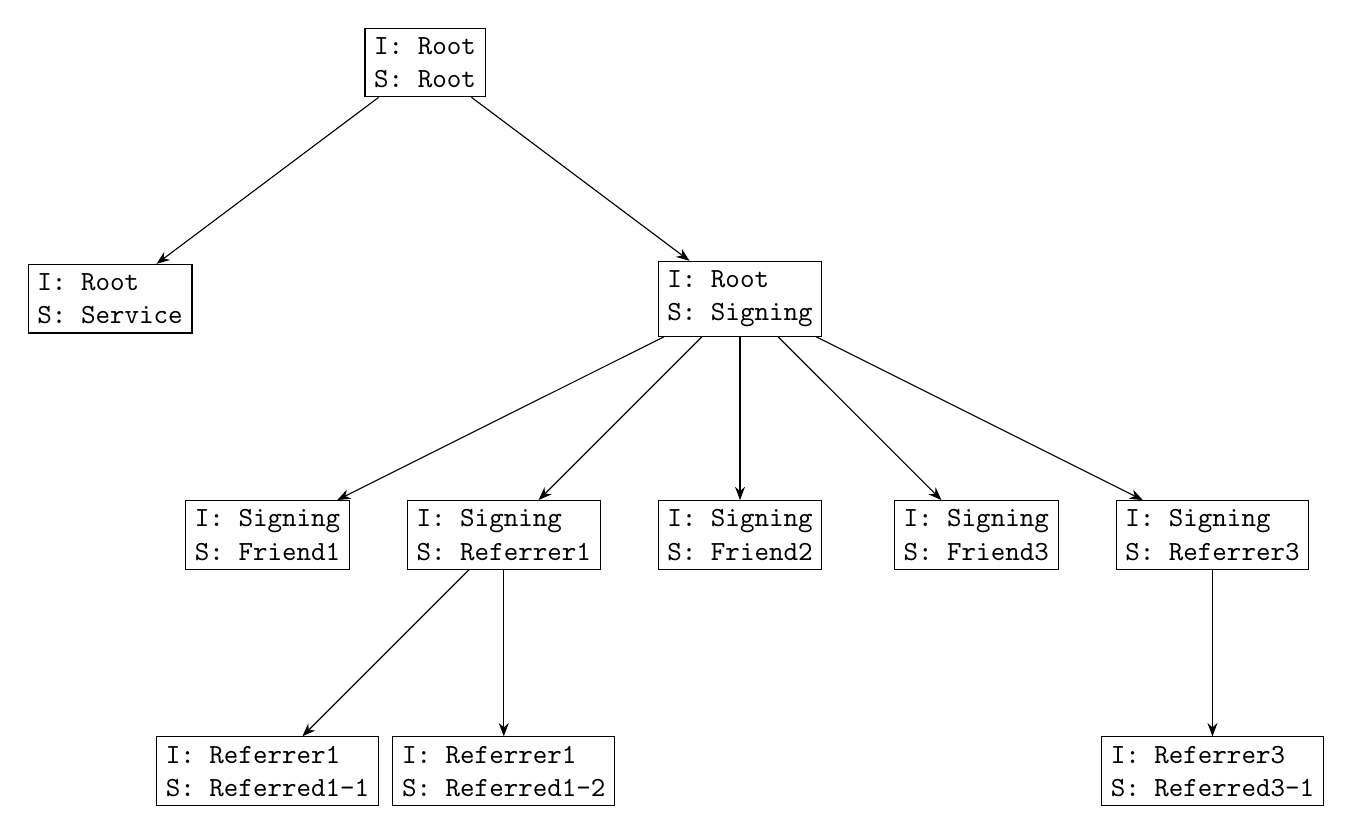
\begin{tikzpicture}
	\node (Root) at (0, 0) [align=left,draw] {\texttt{I: Root} \\ \texttt{S: Root}};

	\node (Service) at ($(Root) + (-4, -3)$) [align=left,draw] {\texttt{I: Root} \\ \texttt{S: Service}};
	\node (Signing) at ($(Root) + (4, -3)$) [align=left,draw] {\texttt{I: Root} \\ \texttt{S: Signing}};
	\draw[-Stealth] (Root) -- (Service);
	\draw[-Stealth] (Root) -- (Signing);

	\node (Friend1) at ($(Signing) + (-6, -3)$) [align=left,draw] {\texttt{I: Signing} \\ \texttt{S: Friend1}};
	\node (Referrer1) at ($(Signing) + (-3, -3)$) [align=left,draw] {\texttt{I: Signing} \\ \texttt{S: Referrer1}};
	\node (Friend2) at ($(Signing) + (0, -3)$) [align=left,draw] {\texttt{I: Signing} \\ \texttt{S: Friend2}};
	\node (Friend3) at ($(Signing) + (3, -3)$) [align=left,draw] {\texttt{I: Signing} \\ \texttt{S: Friend3}};
	\node (Referrer3) at ($(Signing) + (6, -3)$) [align=left,draw] {\texttt{I: Signing} \\ \texttt{S: Referrer3}};
	%\node (FriendExtra) at ($(Signing) + (9, -3)$) [align=left,draw] {\ldots};
	\draw[-Stealth] (Signing) -- (Friend1);
	\draw[-Stealth] (Signing) -- (Referrer1);
	\draw[-Stealth] (Signing) -- (Friend2);
	\draw[-Stealth] (Signing) -- (Friend3);
	\draw[-Stealth] (Signing) -- (Referrer3);
	%\draw[-Stealth] (Signing) -- (FriendExtra);

	\node (Referred1-1) at ($(Referrer1) + (-3, -3)$) [align=left,draw] {\texttt{I: Referrer1} \\ \texttt{S: Referred1-1}};
	\node (Referred1-2) at ($(Referrer1) + (0, -3)$) [align=left,draw] {\texttt{I: Referrer1} \\ \texttt{S: Referred1-2}};
	%\node (Referred1-Extra) at ($(Referrer1) + (3, -3)$) [align=left,draw] {\ldots};
	\node (Referred3-1) at ($(Referrer3) + (0, -3)$) [align=left,draw] {\texttt{I: Referrer3} \\ \texttt{S: Referred3-1}};
	\draw[-Stealth] (Referrer1) -- (Referred1-1);
	\draw[-Stealth] (Referrer1) -- (Referred1-2);
	%\draw[-Stealth] (Referrer1) -- (Referred1-Extra);
	\draw[-Stealth] (Referrer3) -- (Referred3-1);
\end{tikzpicture}
}
\end{makeimage}
\caption{Example AFR PKI.}
\end{figure}
\end{center}

Having the infrastructure drawn out, the next thought on my mind was: how am I going to convince myself that the infrastructure is viable?  The answer that I chose was to speculate various \emph{use cases} that I would want to apply to the infrastructure.  I could then write test cases for each of the various use cases in order to convince myself of the infrastructure's integrity.  While I was brainstorming the use cases, it became clear to me that there was a useful distinction between the \emph{reason} for a use case and the \emph{mechanism} for fulfilling that use case; for example, the admin may wish to invite a friend (the reason), but this is accomplished by issuing a friend's client certificate (the mechanism).  Hence I decided to name all of my use cases by their mechanism, knowing that each may have multiple reasons for being used.  The list was as follows:
\begin{enumerate}
	\item Initialize
	\item Generate friend client cert
	\item Revoke friend client cert
	\item Generate friend signing cert
	\item Revoke friend signing cert
	\item Revoke referral client cert
	\item Friend revokes referral
	\item Friend revokes their client cert
	\item Friend revokes their signing cert
	\item Referred revokes their client cert
	\item Re-generate service cert
	\item Re-generate signing CA
\end{enumerate}
The terminology wasn't quite at its final form, and I completely forgot about friends issuing client certificates with their referrer certificate, but this provided a good basis for designing tests.  I decided to design tests around use cases 1 through 10, omitting the disaster scenarios in the last two use cases on the grounds that they were too much for the current version of the tooling.  I also wrote the tests to include not just a check for success but also a so-called ``parity'' check; for example, checking that a valid client certificate is authorized but also, as ``parity'', checking that an invalid client certificate is unauthorized in order to ensure that the service isn't accepting any random certificate.  The 10 uses cases and their tests thus became:
\begin{enumerate}
	\item Initialize
	\begin{itemize}
		\item Verify service certificate works
		\item Verify signing key works via using admin client cert
		\item Verify unauthorized service certificate rejected
		\item Verify unauthorized client cert rejected
	\end{itemize}
	\item Generate friend client cert
	\begin{itemize}
		\item Verify friend can connect
		\item Uncertified cert fails
	\end{itemize}
	\item Revoke friend client cert
	\begin{itemize}
		\item Revoked friend can no longer connect
		\item Non-revoked friend can connect.
	\end{itemize}
	\item Generate friend signing cert
	\begin{itemize}
		\item Referred can connect
		\item Unverified cert fails
	\end{itemize}
	\item Revoke friend signing cert
	\begin{itemize}
		\item Referred can no longer connect
		\item Other referred can connect
	\end{itemize}
	\item Admin Revoke referral client cert
	\begin{itemize}
		\item Referred can no longer connect
		\item Other referred can still connect
	\end{itemize}
	\item Friend revokes referral
	\begin{itemize}
		\item Referred can no longer connect
		\item Other referred can connect
	\end{itemize}
	\item Friend revokes their client cert
	\begin{itemize}
		\item Friend can no longer connect
		\item Other friend can connect
	\end{itemize}
	\item Friend revokes their signing cert
	\begin{itemize}
		\item Referred can no longer connect
		\item Other referred (from different friend) can connect
	\end{itemize}
	\item Referred revokes their client cert
	\begin{itemize}
		\item Referred can no longer connect
		\item Other referred (from same friend) can connect
	\end{itemize}
\end{enumerate}
Plans thus written out, it was time to implement the tests.

\subsection{Implementing Tests}
While an abstract implementation of AFR tests might have used just the OpenSSL \texttt{s_server} directly, my main concern was getting AFR to work properly with InspIRCd, hence I added the tests to my \htmladdnormallink{inspircdtests}{https://github.com/clinew/inspircdtests} repo which was written, intuitively enough, against InspIRCd.  Since each test involved a large amount of state, I decided to set-up state at the beginning of the tests and re-use it across the entire suite of tests; this meant that subsequent tests were allowed to depend on previous tests.  I also settled on ``referrer'' and ``referred'' terminology around this time, allowing me to succinctly refer to tests with names such as ``sign-referrer''.  Actually implementing the tests according to plan went smoothly, until I ran into ``revoke-referred''.

The purpose of the ``revoke-referred'' test was to allow an admin to ban a referred user without having to wait for the referrer to issue a Certificate Revocation List (CRL) for the user.  I had thought that I'd be able to use Indirect CRLs in order to easily implement this test, but I couldn't figure out how to actually do this, so I started searching and running into similar but irrelevant posts.  For example, \htmladdnormallink{this issue}{https://github.com/openssl/openssl/issues/2358} seemed to me to be an issue with how CRLs were searched for, not how to issue indirect CRLs.  \htmladdnormallink{This question}{https://security.stackexchange.com/questions/91680/how-to-trust-a-ca-to-sign-a-crl-but-not-a-cert} was similar to my need, but did not explain how to generate an indirect CRL.  \htmladdnormallink{This lone question}{https://superuser.com/questions/1273121/how-to-verify-indirect-crl} appears to focus on verification, but, without generation, is not useful to me.  Most hopeful was this \htmladdnormallink{old forum post}{http://openssl.6102.n7.nabble.com/Re-openssl-org-3097-Incorrect-revocation-status-with-indirect-CRL-td47482.html} which provided an example of an indirect CRL, but in this case the example appeared to to rely on the fact the indirect CRL issuer was only issuing CRLs for a particular CA and not multiple CAs (the latter being my requirement); nonetheless I \htmladdnormallink{tried}{https://github.com/clinew/inspircdtests/tree/indirect_crl} to get example working but didn't meet with any success.  While nothing solved my specific need, I did, however, learn from \htmladdnormallink{this post}{https://stackoverflow.com/questions/9104108/is-serial-number-a-unique-key-for-x509-certificate} that the purpose of the serial number is to uniquely identify a certificate issued by a given CA.  For the rest, I took some time to study \htmladdnormallink{the RFC}{https://tools.ietf.org/html/rfc5280#section-5} and hypothesize a way forward.

Since I couldn't figure out how to implement ``revoke-referred'' properly, I came up with a stop-gap test instead.  While there didn't appear to be a way to ban client certificates globally in InspIRCd, it was possible to ban a given certificate fingerprint on a channel, so I designed a test that would have a user join a temporary channel, set a ban on the channel for the certificate fingerprint of the other user, then have the other user attempt to join the channel and fail; for parity, a third user who wasn't banned on the channel would then join the channel successfully.  Plan in hand, I attempted this only to find that whenever I joined the temporary channel I would not be an operator as I expected, thus I couldn't set any bans on the channel.  After a bit of searching I found that my test server's InspIRCd \texttt{options} tag was set with \texttt{defaultmodes="nt"} when it should have been \texttt{defaultmodes="not"}, talk about Murphy's Law!  Fixing this issue allowed me to set a ban on the channel and implement the test.

Implementing the next test went smoothly, but I then realized that there wasn't much point to implementing the last three tests (``friend-revoke-client'', ``friend-revoke-referrer'', and ``referred-revoke-client'') at this time, since there does not appear to be a way for users to self-revoke their certificates, and having the admin revoke the friend certificates (for the former two) and the friend revoke the referred certificate (for the latter-most) would simply be a repeat of previous tests.  These tests would make sense if I had some kind of network protocol for certificate management and could mimic a client authenticating with their certificate and requesting a revocation on the given certificate, but they did not appear useful as tests with the current implementation.

With tests implemented which verified that the infrastructure appeared to work as I expected (besides the indirect CRLs), I began to look ahead to actually deploying this infrastructure.  Given the sheer volume of complex commands I had to issue for testing, I decided that there was no way that I could realistically run these commands by hand and be sure that I had done the same as in my tests.  I would have to develop tools in order to simplify my work for me.

\subsection{Implementing Tooling}
One of the more perplexing choices when writing tooling is balancing the amount effort to put into tooling development against the benefits gained from having tooling.  With regards to AFR tooling, the main benefit for me was reproduceability from not having to run a series of complex commands by hand for common use cases.  Since the tools would be calling OpenSSL commands, I decided to write the tooling in \texttt{bash}; as much as I generally prefer Python's data structures and control flow, I find the \texttt{subprocess} module's interface to be extremely awkward and cumbersome.  Given the issue mentioned earlier with the lack of a command-line interface for generating indirect CRLs, I also suspected that future versions of the tooling would need a re-write in a language, possibly C, that had bindings for the OpenSSL library, so I decided not to put a large amount of effort into the tooling; ``good enough'' would suffice.

The next choice I had was where to put everything.  After consulting the \htmladdnormallink{Filesystem Hierarchy Standard v3}{https://refspecs.linuxfoundation.org/FHS_3.0/fhs/index.html}, I settled on \texttt{/var/lib/afr/instance}, where \texttt{instance} might one day allow multiple independent AFR PKIs; though I would be exposing some information in that directory to consumers, the \texttt{/srv} path felt like it was more for Web services.  System AFR configuration would go to \texttt{/etc/afr/afr.conf}, and I also ended up sticking the OpenSSL configuration file in the same directory path, though, in retrospect, \texttt{/usr/lib/share/afr} might have been more appropriate.

Layout in place, I began to implement the basic admin use cases, and found that I needed to add auxiliary commands in order to implement parts of certain uses cases; for example \texttt{receive-crl} in order to apply a CRL from a referrer certificate.  Once the admin use cases were done, I then had to figure out how to implement the use cases for friends and referreds.  While it might have been possible to add non-admin-specific subcommands, giving them names such as \texttt{friend-init} and \texttt{friend-revoke-referred} would be cumbersome for users to type and users would be liable to conflate non-admin subcommands with admin subcommands such as the regular \texttt{init}.  The solution that I chose was to add a separate \texttt{afrc} command for \emph{clients} with its own set of subcommands; functionality common to both \texttt{afr} and \texttt{afrc} would be put into \texttt{afr_lib.sh} and both friends and referreds would use the same command set due to the similarities between the two users.  I then implemented the subcommands needed for client use cases, although the implementation I used was slightly awkward since I forced clients to use \texttt{make install} in order to place \texttt{afr_lib.sh} and \texttt{openssl.cnf} in expected locations, but I hadn't thought up a particularly easy workaround for that and it was ``good enough''.

A trick that I used in order to convince myself of the basic robustness of my tooling was to refactor the AFR tests that I'd written for InspIRCd to use the new AFR utilities.  With each AFR subcommand implemented, I'd refactor the test to use the corresponding subcommand rather than raw OpenSSL commands.  Thus, by the time I'd finished writing the tooling, I had tests that verified the tooling and the PKI!  While this was good news for when I deployed a new AFR PKI, I still had to figure out how I was going to migrate from my existing PKI to the new AFR PKI.

\subsection{Transition Plan Development}
While I could have immediately migrated from my existing PKI to a new AFR PKI, doing so would have invalidated all of my PKI's existing client certificates, making all of my non-existent users unhappy and leaving me discontent with my computer skills.  As such, I decided to look into a subject which I was not yet familiar with: \htmladdnormallink{cross-signing}{https://en.wikipedia.org/wiki/X.509#Certificate_chains_and_cross-certification}.  \htmladdnormallink{This paper}{http://www.oasis-pki.org/pdfs/Understanding_Path_construction-DS2.pdf} in particular provided much insight into the process.  I learned that, contrary to my previous belief, cross-signing could be used in order to build a distributed trust model and not just a hierarchical model.  I also began to think that it might be possible to create a transitional PKI that would accept both old and new client certificates, and possibly allow users with the old and new root as a trust anchor to authenticate the service.  Though I also realized that I had made an elementary mistake with my client certificates.

I'm not sure why it took reading about cross-certification for this vulnerability to occur to me, but, as I studied path construction, I realized that the AFR PKI had nothing in it that would prevent a referrer certificate from issuing server certificates!  D'oh.  Thankfully, the solution was straightforward enough: add a critical extension to the signing and all referrer certificates which only authorizes those certificates for client authentication; specifically: \texttt{extendedKeyUsage=critical,clientAuth}.  Strangely enough, the RFC section on \htmladdnormallink{Extended Key Usage}{https://tools.ietf.org/html/rfc5280#section-4.2.1.12} states that: ``In general, this extension will appear only in end entity certificates.''.  This caused me a bit of worry, since a malicious referrer could leave off the extension on an issued service certificate, but thankfully my \htmladdnormallink{test}{https://github.com/clinew/inspircdtests/commit/80bc6dd3d6005a0bba877d2d557936aa0e00a7e4} showed that the extension was effective despite not being on the end-entity certificate.  With that fixed, I could then begin brainstorming a transitional PKI.

The previous PKI (v0.1.0) I had referred to as ``Friend-of-Friend'' and was structured as such:
\begin{center}
\begin{figure}
\begin{makeimage}
\fbox{
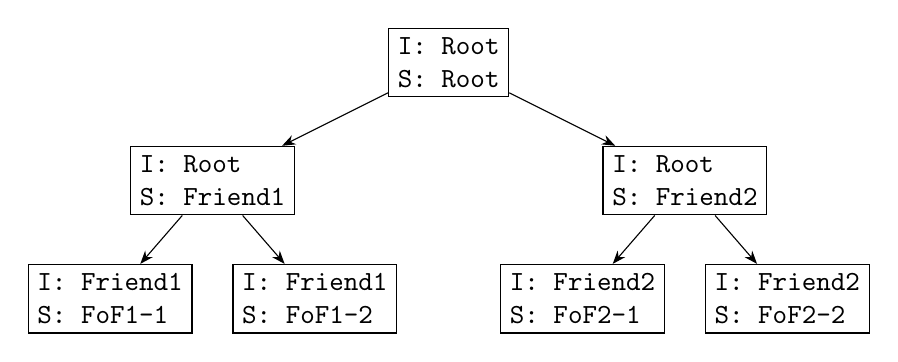
\begin{tikzpicture}
	\node (Root) at (0, 0) [align=left,draw] {\texttt{I: Root} \\ \texttt{S: Root}};
	\node (Friend1) at ($(Root) + (-3, -1.5)$) [align=left,draw] {\texttt{I: Root} \\ \texttt{S: Friend1}};
	\node (Friend2) at ($(Root) + (3, -1.5)$) [align=left,draw] {\texttt{I: Root} \\ \texttt{S: Friend2}};
	\node (FoF1-1) at ($(Friend1) + (-1.3, -1.5)$) [align=left,draw] {\texttt{I: Friend1} \\ \texttt{S: FoF1-1}};
	\node (FoF1-2) at ($(Friend1) + (1.3, -1.5)$) [align=left,draw] {\texttt{I: Friend1} \\ \texttt{S: FoF1-2}};
	\node (FoF2-1) at ($(Friend2) + (-1.3, -1.5)$) [align=left,draw] {\texttt{I: Friend2} \\ \texttt{S: FoF2-1}};
	\node (FoF2-2) at ($(Friend2) + (1.3, -1.5)$) [align=left,draw] {\texttt{I: Friend2} \\ \texttt{S: FoF2-2}};
	\draw[-Stealth] (Root) -- (Friend1);
	\draw[-Stealth] (Root) -- (Friend2);
	\draw[-Stealth] (Friend1) -- (FoF1-1);
	\draw[-Stealth] (Friend1) -- (FoF1-2);
	\draw[-Stealth] (Friend2) -- (FoF2-1);
	\draw[-Stealth] (Friend2) -- (FoF2-2);
\end{tikzpicture}
}
\end{makeimage}
\caption{The old version (v0.1.0) of the PKI, named ``Friend-of-Friend''}
\end{figure}
\end{center}
As mentioned earlier, my main concern was authorizing old client certificates.  Having clients who trusted the old root certificate be able to trust the new service certificate would be a plus, though.

After a bit of contemplation, I realized that I could authorize friends using client certificates issued by the old PKI by signing the old root certificate as a referrer certificate.  As a downside, any friend-of-friend certificates issued by friends wouldn't be authorized due to the \texttt{pathlen:0} restriction on the cross-signed old root certificate, but no one had yet bothered to use that feature (surprisingly, users don't like typing in esoteric OpenSSL commands) so the solution was ``good enough''.  This then gave the following series of PKI paths:
\begin{center}
\begin{figure}
\begin{makeimage}
\newlength{\tmp}
\settowidth{\tmp}{\texttt{I: New Root CA}}
\fbox{
\begin{tabular}{l|l|l}
Old: & Transition: & New: \\
\begin{tikzpicture}
	\node (Root) at (0, 0) [align=left,draw] {\parbox{\tmp}{\texttt{I: Old Root CA} \\ \texttt{S: Old Root CA}}};
\end{tikzpicture}
&
\begin{tikzpicture}
	\node (NewRoot) at (0, 0) [align=left,draw] {\parbox{\tmp}{\texttt{I: New Root CA} \\ \texttt{S: New Root CA}}};
	\node (Signing) at ($(NewRoot) + (0, -1.5)$) [align=left,draw] {\parbox{\tmp}{\texttt{I: New Root CA} \\ \texttt{S: Signing CA}}};
	\node (OldRoot) at ($(Signing) + (0, -1.5)$) [align=left,draw] {\parbox{\tmp}{\texttt{I: Signing CA} \\ \texttt{S: Old Root CA}}};
	\draw[-Stealth] (NewRoot) -- (Signing);
	\draw[-Stealth] (Signing) -- (OldRoot);
\end{tikzpicture}
&
\begin{tikzpicture}
	\node (NewRoot) at (0, 0) [align=left,draw] {\parbox{\tmp}{\texttt{I: New Root CA} \\ \texttt{S: New Root CA}}};
	\node (Signing) at ($(NewRoot) + (0, -1.5)$) [align=left,draw] {\parbox{\tmp}{\texttt{I: New Root CA} \\ \texttt{S: Signing CA}}};
	\draw[-Stealth] (NewRoot) -- (Signing);
\end{tikzpicture}
\end{tabular}
}
\end{makeimage}
\caption{Paths of the various PKI implementations with regards to trusted certificates when validating client certificates.}
\end{figure}
\end{center}
The old root could then either be cross-signed for a limited duration or revoked by the new signing certificate when the transition period was over; I chose the latter for finer control as circumstance permitted.  Another benefit of signing the old root as a referrer was that any friend-of-friend certificates pretending to be a service would, to my knowledge, not be accepted due to the constraints extension on the signing certificate, though I did not test this.

Configuring the service such that clients who trusted both the old root and the new root would be able to authorize the service was a bit trickier.  This is in part because the validation path would branch depending on which trust anchor the client was using, and the trust anchor would in either case be outside of the certificates sent by the server.  The trick here was to have the old root certificate sign the new root certificate, then have the server present both the cross-signed new root certificate and the service certificate:
\begin{center}
\begin{figure}
\begin{makeimage}
\settowidth{\tmp}{\texttt{I: New Root CA}}
\fbox{
\begin{tabular}{l|l|l}
Old: & Transition: & New: \\
\begin{tikzpicture}
	\node (Root) at (0, 0) [align=left,draw] {\parbox{\tmp}{\texttt{I: Old Root CA} \\ \texttt{S: Old Root CA}}};
	\node[left,text=green!60!black] (Trusted) at (Root.west) {trusted};
	\draw (Root) -- (Trusted);
\end{tikzpicture}
&
\begin{tikzpicture}
	\node (OldRoot) at (0, 0) [align=left,draw] {\parbox{\tmp}{\texttt{I: Old Root CA} \\ \texttt{S: Old Root CA}}};
	\node[left,text=green!60!black] (OldTrusted) at (OldRoot.west) {\parbox{1.1cm}{\centering old \\ trusted}};
	\node (NewRoot) at (6, 0) [align=left,draw] {\parbox{\tmp}{\texttt{I: New Root CA} \\ \texttt{S: New Root CA}}};
	\node[left,text=green!60!black] (NewTrusted) at (NewRoot.west) {\parbox{1.1cm}{\centering new \\ trusted}};
	\node (CrossRoot) at ($(OldRoot) + (1.5, -1.5)$) [align=left,draw] {\parbox{\tmp}{\texttt{I: Old Root CA} \\ \texttt{S: New Root CA}}};
	\node (Service) at ($(CrossRoot) + (1.5, -1.5)$) [align=left,draw] {\parbox{\tmp}{\texttt{I: New Root CA} \\ \texttt{S: Service}}};
	\draw[-Stealth] (OldRoot) -- (CrossRoot);
	\draw[-Stealth] (NewRoot) -- (Service);
	\draw[-Stealth] (CrossRoot) -- (Service);
	% Server-supplied box
	\begin{scope}[on background layer]
		\node (Supplied) [rectangle,thick,draw=white!40!black,inner sep=0.5cm,fit=(Service) (CrossRoot)] {};
		\node [above right,text=white!40!black] at (Supplied.south west) {server-supplied};
	\end{scope}
\end{tikzpicture}
&
\begin{tikzpicture}
	\node (Root) at (0, 0) [align=left,draw] {\parbox{\tmp}{\texttt{I: New Root CA} \\ \texttt{S: New Root CA}}};
	\node[left,text=green!60!black] (Trusted) at (Root.west) {trusted};
	\node (Service) at ($(Root) + (0, -1.5)$) [align=left,draw] {\parbox{\tmp}{\texttt{I: New Root CA} \\ \texttt{S: Service}}};
	\draw[-Stealth] (Root) -- (Service);
\end{tikzpicture}
\end{tabular}
}
\end{makeimage}
\caption{Paths of the various PKI implementations with regards to client trust of the server.}
\end{figure}
\end{center}
No matter which root certificate the client would use as a trust anchor, there would be a valid path to that trust anchor.  Also of interest is the fact that cross-signing \emph{client} certificates meant that the \emph{new} root had to certify the \emph{old} root, but cross-signing the \emph{server} certificate meant that the \emph{old} root had to certify the \emph{new} root.

Naturally, I wanted to make sure that the planned infrastructure actually worked, so I wrote some \htmladdnormallink{transition tests}{https://github.com/clinew/inspircdtests/blob/master/ssl_transition.sh} for that purpose; in addition to verifying that old and new certificates worked with the transition PKI, I made sure to check that new certificates did not work with the old PKI.  I did have some worries that the client software which trusted the new root would not authenticate the server due to the extraneous, cross-signed certificate sent by the server, but, to my relief, the tests showed otherwise.  All of the tests ended up passing as I had hoped.

One last thing that I did in order to help remind users to transition was to write a \htmladdnormallink{quick, hacky patch}{https://github.com/clinew/inspircd/commit/a73361a4e3f7a2e51a7e64c7cd948c4a422846d2} that would warn users with old client certificates that they should upgrade them.  Finally, since the tests were were functional and the tooling was in place, I decided that it was time to deploy the changes.

\subsection{Deploying and Documenting}
Since I wanted to deploy my changes in the smoothest manner possible, I took some time to come up with a series of steps that would fulfill that purpose.  In addition to updating certificates, I had to do a couple of housekeeping tasks such as: update \htmladdnormallink{user connection instructions}{https://github.com/clinew/frostsnow.net/blob/master/instructions.tex}, add a root certificate location, and plan for a full transition.  Taking all of these into consideration, I then planned and executed the following series of steps: revising the user connection instructions, generating the new AFR root, generating the transitional certificates, configuring InspIRCd to use the transitional certificates, deploying the transitional certificates, updating the website with the revised connection instructions and the new AFR root, backing up the AFR root key in an offline location, scheduling a full transition time in the InspIRCd Message of the Day (MotD), and finally migrating the users which I owned to the new client certificates.  Thankfully, there were no surprises when I actually did this series of steps.

With the server running the new AFR PKI, all that remained was me for to document my work.  You know, so I can use it to pick up women at bars.  Posteriority.  Or something.  To this end, I decided to write a \htmladdnormallink{\LaTeX white paper}{https://github.com/clinew/afr/blob/master/doc/afr.tex} and add it to the \htmladdnormallink{AFR tools}{https://github.com/clinew/afr} \texttt{doc} directory.  I then realized that, much to my annoyance, re-configuring my test environment to use AFR had broken my hacky InspIRCd tests, so I wrote a \htmladdnormallink{commit}{https://github.com/clinew/inspircdtests/commit/ce823ad6eb704cf0dc07a7d2036542b54a6cdded} to fix them; perhaps one day I'll implement an elegant solution to manage test environment configuration.  Last of all, I wrote (am writing?) this blog in order to finish documenting my work; this was most useful for the transitional PKI, since that fell outside of the scope of the AFR white paper.

There's still a bunch of work that I'd like to do on AFR in order to get it into something that might actually be generally useful for people.  First and foremost will be figuring out whether I can actually even use indirect CRLs in a manner which suits my needs; if not, the whole scheme may fall apart without some clever alterations.  After that, usability will be key.  This may mean writing a network protocol, integrating AFR with a technology such as PAM, or writing some kind of wizard program.  While I'm glad to have this version complete, there's still plenty of work to be done.


% Replacing an Encrypted Hard Drive on a RAID-5 Array
\section{2020-04-12 Replacing an Encrypted Hard Drive on a RAID-5 Array}
This\label{2020-04-12-replacing-hard-drive} blog entry is about my attempt to replace a failing drive on my home server's amateur-encrypted RAID-5 arrays.  While replacing a failing drive isn't particularly difficult, it must be done with care, and my situation was complicated by the \htmladdnormallink{encryption scripts}{https://github.com/clinew/gscripts} I had set-up around the array.  Yet, even this was not the end of my troubles, as an unexpected problem arose in the middle of my work.

\subsection{Troubleshooting with S.M.A.R.T.}
For the past couple of months, message similar to the following had been appearing in my log about once every other week:

\begin{verbatim}
[5799854.385960] sd 1:0:0:0: [sdb] tag#0 FAILED Result: hostbyte=DID_OK driverbyte=DRIVER_SENSE
[5799854.385964] sd 1:0:0:0: [sdb] tag#0 Sense Key : Medium Error [current]
[5799854.385968] sd 1:0:0:0: [sdb] tag#0 Add. Sense: Unrecovered read error - auto reallocate failed
[5799854.385972] sd 1:0:0:0: [sdb] tag#0 CDB: Read(10) 28 00 00 84 43 28 00 00 08 00
[5799854.385976] blk_update_request: I/O error, dev sdb, sector 8667947 op 0x0:(READ) flags 0x80700 phys_seg 1 prio class 0
[5799855.795885] sd 1:0:0:0: [sdb] tag#0 FAILED Result: hostbyte=DID_OK driverbyte=DRIVER_SENSE
[5799855.795889] sd 1:0:0:0: [sdb] tag#0 Sense Key : Medium Error [current]
[5799855.795893] sd 1:0:0:0: [sdb] tag#0 Add. Sense: Unrecovered read error - auto reallocate failed
[5799855.795897] sd 1:0:0:0: [sdb] tag#0 CDB: Read(10) 28 00 00 84 43 28 00 00 08 00
[5799855.795901] blk_update_request: I/O error, dev sdb, sector 8667947 op 0x0:(READ) flags 0x4000 phys_seg 1 prio class 0
[5799856.020331] md/raid:md0: read error corrected (8 sectors at 8667944 on dm-17)
\end{verbatim}

After a couple of months the messages began to appear daily, whenever I would perform the daily system updates.  While viewing \texttt{/proc/mdstat} showed the drive as "up", I figured it would be best to replace it sooner rather than later.  Before doing that, though, I decided to play around with the \htmladdnormallink{S.M.A.R.T.}{https://en.wikipedia.org/wiki/S.M.A.R.T.} capabilities of the drive in order to see if they would diagnose the drive as in a pre-failure state.   To begin, I decided to check the health self-assessment with the \texttt{-H} option to \texttt{smartctl}:

\begin{verbatim}
hesse /home/frostsnow # smartctl -H /dev/sdb
smartctl 7.0 2018-12-30 r4883 [x86_64-linux-5.4.13] (local build)
Copyright (C) 2002-18, Bruce Allen, Christian Franke, www.smartmontools.org

=== START OF READ SMART DATA SECTION ===
SMART overall-health self-assessment test result: PASSED
\end{verbatim}

Well, the health status said that it was passing, but I wasn't convinced.  Perhaps it hadn't been tested?  I next ran a short self-test:

\begin{verbatim}
/hesse /home/frostsnow # smartctl -t short /dev/sdb
smartctl 7.0 2018-12-30 r4883 [x86_64-linux-5.4.13] (local build)
Copyright (C) 2002-18, Bruce Allen, Christian Franke, www.smartmontools.org

=== START OF OFFLINE IMMEDIATE AND SELF-TEST SECTION ===
Sending command: "Execute SMART Short self-test routine immediately in off-line mode".
Drive command "Execute SMART Short self-test routine immediately in off-line mode" successful.
Testing has begun.
Please wait 2 minutes for test to complete.
Test will complete after Sun Mar 29 16:43:35 2020

Use smartctl -X to abort test.
\end{verbatim}

This short test didn't show any errors, so I ran it again out of perplexity, which also didn't show any errors, and then decided to run the longer self-test:

\begin{verbatim}
hesse /home/frostsnow # smartctl -t long /dev/sdb
smartctl 7.0 2018-12-30 r4883 [x86_64-linux-5.4.13] (local build)
Copyright (C) 2002-18, Bruce Allen, Christian Franke, www.smartmontools.org

=== START OF OFFLINE IMMEDIATE AND SELF-TEST SECTION ===
Sending command: "Execute SMART Extended self-test routine immediately in off-line mode".
Drive command "Execute SMART Extended self-test routine immediately in off-line mode" successful.
Testing has begun.
Please wait 36 minutes for test to complete.
Test will complete after Sun Mar 29 17:20:09 2020

Use smartctl -X to abort test.
\end{verbatim}

Much to my satisfaction, the long test actually reported a read error:

\begin{verbatim}
hesse /home/frostsnow # smartctl -l selftest /dev/sdb
smartctl 7.0 2018-12-30 r4883 [x86_64-linux-5.4.13] (local build)
Copyright (C) 2002-18, Bruce Allen, Christian Franke, www.smartmontools.org

=== START OF READ SMART DATA SECTION ===
SMART Self-test log structure revision number 1
Num  Test_Description    Status                  Remaining  LifeTime(hours)  LBA_of_first_error
# 1  Extended offline    Completed: read failure       40%     54064         865226
# 2  Short offline       Completed without error       00%     54064         -
# 3  Short offline       Completed without error       00%     54064         -
# 4  Short offline       Completed without error       00%         0         -
\end{verbatim}

Having now recorded an error during one of its self-tests, perhaps the health self-assessment would now report a failure?

\begin{verbatim}
hesse /home/frostsnow # smartctl -H /dev/sdb
smartctl 7.0 2018-12-30 r4883 [x86_64-linux-5.4.13] (local build)
Copyright (C) 2002-18, Bruce Allen, Christian Franke, www.smartmontools.org

=== START OF READ SMART DATA SECTION ===
SMART overall-health self-assessment test result: PASSED
\end{verbatim}

Guess not.  Perhaps, as the \texttt{man} page reads, it will only report failing if the drive has already failed or thinks it will fail within the next 24 hours.  Unfortunately for me, 24 hours isn't sufficient notice for me as I don't have employees working daily in order to service my home computer; I need about a week's notice so that I can plan for the next weekend.  Nice as it would have been to get S.M.A.R.T. to declare that the drive needs replacing, I decided to go ahead and do the replacement anyways.

\subsection{Removing the Old Drive}

The trick to removing and replacing the old drive was to attempt to do so as smoothly as possible, with the shortest downtime and the fewest gotchas as possible.  To this end I developed a step-by-step plan in order to make the process as smooth as possible:

\begin{enumerate}
\item Identify the failing drive
\item Wipe the new drive (already done)
\item Generate a key for the new drive with \texttt{keyfile.sh}
\item Add the key for the new drive to the \texttt{initramfs}
\item Modify \texttt{extlinux.conf} to boot only the two working, pre-existing drives and to boot into single-user mode rather than multi-user mode
\item Power down the server
\item Install the new drive
\item Boot into the server
\item Add the new drive to the array
\item Add the new drive to boot arguments, boot into multi-user mode
\item Restart the server
\end{enumerate}

Simple enough, right?  In order to identify the hard drive, I used the venerable \texttt{hdparm} program to grab the drive's serial number (redacted in the below output):

\begin{verbatim}
hesse /home/frostsnow # hdparm -i /dev/sdb

/dev/sdb:

 Model=Maxtor 6Y080M0, FwRev=YAR51HW0, SerialNo=REDACTED
 Config={ Fixed }
 RawCHS=16383/16/63, TrkSize=0, SectSize=0, ECCbytes=4
 BuffType=DualPortCache, BuffSize=7936kB, MaxMultSect=16, MultSect=off
 CurCHS=16383/16/63, CurSects=16514064, LBA=yes, LBAsects=156250000
 IORDY=on/off, tPIO={min:120,w/IORDY:120}, tDMA={min:120,rec:120}
 PIO modes:  pio0 pio1 pio2 pio3 pio4
 DMA modes:  mdma0 mdma1 mdma2
 UDMA modes: udma0 udma1 udma2 udma3 udma4 udma5 *udma6
 AdvancedPM=yes: disabled (255) WriteCache=enabled
 Drive conforms to: ATA/ATAPI-7 T13 1532D revision 0:  ATA/ATAPI-1,2,3,4,5,6,7

 * signifies the current active mode
\end{verbatim}

From there it was a matter of methodically following the steps that I'd laid out.  Generating a key, patching the \texttt{initramfs}, powering down the server, installing the new drive, booting the server---and, er, wait, what?  See, my particular motherboard is interesting in that, when power is first applied, the fan starts running at maximum speed before turning off when the motherboard enters a standby state.  Well, when I powered on the motherboard, it did the usual fan spin-up, but then, rather than idling, it seemed to cut out, then start again, then cut out, then start again, then cut out\ldots~Crap.  Something was going wrong.

\subsection{Reviving the Motherboard}
Perhaps there was a problem with the new drive?  I tried replacing the old drive to see if it'd boot.  Same problem.  Perhaps I'd jiggled a cable?  I ensured they were all in place.  Same problem.  Perhaps a component was faulty?  I tried disconnecting almost everything except the power to the motherboard itself.  Same problem.  Puzzled, I examined the motherboard, and that's when I noticed three bulging capacitors with leaked\ldots~something on their heads.  Now, this is when a high-budget blog would insert a picture of the bulging capacitors, but this blog is not high-budget and my camera was broken, so, sadly, I have no pictures of the broken caps.  Lesser mortals would have given up and bought a new motherboard, but I decided to be stubborn and see if I could instead replace the capacitors and thus save the board.  I began by removing the board, but as I removed the board from its case I had an unfortunate incident with one the screws which caused the motherboard to make a sort of stretch-cracking sound as I was unscrewing one of the screws;  I decided to try the other screws after this happened, and came back to the painful-noise-making screw last.  On the last incident it didn't make any sound and I was able to pull the board out, but I noticed that the nut under the screw had become stuck and tried to move with the screw, thus pulling the board up when I tried to unscrew it.  Ouch.  I hoped that it hadn't damaged the motherboard.

I then spent some time researching capacitors, since any new domain of knowledge, no matter how simplified, involves a number of considerations that one must take into account before successfully attempting any project in said domain.  In this case, I learned the difference between \htmladdnormallink{through-hole}{https://en.wikipedia.org/wiki/Through-hole_technology} technology and \htmladdnormallink{surface-mount}{https://en.wikipedia.org/wiki/Surface-mount_technology} technology; luckily, my board was using through-hole technology.  I also couldn't help but notice the unfortunate use of "your" in this \htmladdnormallink{old capacitor advertisement}{https://upload.wikimedia.org/wikipedia/commons/5/57/Radio_Times_-_1923-12-28_-_page_39_-_Dubilier.png}.  Finding no other details relevant to my issue, I then took a q-tip to clean my capacitors and then tried to glean off as much information as possible from them so that I could figure out what to replace them with.  Turns out that all the capacitors were manufactured by Rubycon, model MBZ, and were spec'd for 3300uF at 6.3V with what is presumably a maximum temperature of 105 degrees Celsius.  Well, I couldn't find the model specified listed on the \htmladdnormallink{Rubycon website}{http://www.rubycon.co.jp/en/index.html}, but I did find what is \htmladdnormallink{presumably a legitimate data sheet}{https://pdf1.alldatasheet.com/datasheet-pdf/download/144891/RUBYCON/MBZ.html} on the capacitor from a random website I found by searching; the data sheet claimed that the capacitor had a 20\% tolerance, which was the last missing piece of information I'd need for a replacement.

Information in hand, I tried a couple of local stores, such as \htmladdnormallink{PCH Cables}{https://www.pchcables.com/} and \htmladdnormallink{Surplus Gizmos}{https://www.surplusgizmos.com/}; none of them had what I needed, though Surplus Gizmos could sell me used motherboards with the same capacitors, I was not keen to essentially double the complexity of my replacement project.  \htmladdnormallink{URS Electronics}{https://www.ursele.com/} also did not have any of the capacitors listed.  The capacitor manufacturer themselves seemed to only operate in bulk orders, which is understandable since individual capacitors are cheap and tend to be a bulk product.  Local and direct options exhausted, I was able to find someone selling the exact same brand of capacitor off of Amazon in sets of 8, and so decided to buy from them; they arrived in a few days, pleasantly beating my expectation of having to wait another week.  For the soldering station I'd need, a frien-quaintance was kind enough to give me their old one, along with some solder, flux, and desoldering braid.  By the time I'd acquired everything, it was about 9 p.m. on Sunday evening, a week after I had first powered-off my server (so much for minimizing downtime).  Heedless of the time, I wanted my board fixed that weekend and thus began working on it.

This was my second time soldering, ever, and I'd never desoldered before.  Ever cautious, I slowly turned the heat on the station up to max after having no luck with the lower temperatures.  Unsure how to use the braid to properly remove the solder with the capacitors in there, I wiggled the capacitors out by heating one of the two holes at a time and then pulling on the capacitor; this eventually succeeded in getting the capacitors out, but left a hole full of solder that was no good for inserting capacitors into.  Now the real frustration began for me.  I had a very difficult time getting the braid to remove the solder in the holes.  After getting frustrated and doing some searching, I learned to apply the flux to the braid; that seemed to help, but it didn't seem to be enough to fully clean the hole and got gunk all around the hole.  After about 3-4 hours of this it was about 2 a.m. and I only had half of the six holes cleaned.  I feel asleep exhausted and frustrated.  The next morning I took a closer look at the soldering iron in the daylight and noticed that either there was some crud on part of the tip or that it had been worn away; either way, a small part of the tip seemed to be effectively heated while the other bit remained cool.  Taking this into account, I attempted to desolder with the hot part of the tip at lunch.  After a few attempts, I removed most of the solder from the 4th hole, and a bit more from the last two holes, which didn't have much in them anyways.  After the holes were cleared, I took care to align the capacitors and resolder them, which was much easier than desoldering them, though most of them came out a little crooked.

Before powering the motherboard on, I attempted to remove the gunk on the board with some rubbing alcohol, though the shop rags I was using left traces of red fiber anyways.  Now, at this point I was rather\ldots~hesitant about my chance for success.  The board had made those terrible sounds thanks to that evil nut on the screw, I'd run a hot soldering iron against the board a number of times because I couldn't hold my hand steady (not to mention any remaining gunk I might have left on the board), and the capacitors being broken might have caused severe electrical damage to the board anyways.  Nonetheless, the only thing to do was to try anyways.  I found the motherboard \htmladdnormallink{product guide}{https://www.intel.com/content/dam/support/us/en/documents/boardsandkits/desktop-boards/965/DQ965GF/DQ965GF_ProductGuide03.pdf} online so that I could figure out how to re-attach all of the basic connectors, plugged everything in, powered on the board, and watched as the fan ran, stopped\ldots~and stayed stopped.  Was it\ldots~working?  I powered off the board, re-attached the other connectors such as the VGA output and SATA cables, powered on the board and, amazingly, the motherboard was actually working again!  Now I could get back to replacing that hard drive.

\subsection{Adding the New Drive}
I began drive replacement by attempting to remove the old drive with \texttt{mdadm --manage /dev/md0 -r detached}; I think that did something.  Next thing, I noticed that I had forgotten to take into account setting up an encrypted mapping for the new drive; I had the \texttt{initramfs} on my server, but I hadn't installed the \texttt{cpio} utilities in order to extract the scripts I'd need to create the mapping, so I extracted them from another machine and then moved them onto the server.  Once I had the scripts, I used \texttt{cryptsetup.sh} command with the previously-generated key in order to create a mapping, though it accepted the password as a command-line argument rather than some secure method (the scripts could use a refactor), so I cleared my history with \texttt{history -c} afterwards.  Once I had the mapping set-up, I added the encrypted drive mapping to the array with \texttt{mdadm --manage /dev/md0 --add /dev/mapper/NAME}.  This seemed to work and the array began rebuilding.  Satisfied, I reconfigured \texttt{extlinux.conf} to boot with the new drive and rebooted the machine (with the ethernet cable detached).  When it came up, I then logged in as a regular user and ran \texttt{watch cat /proc/mdstat} in order to watch the array rebuild itself.  A little after midnight, the array was rebuilt and I was able to bring the server back to normal operation!

And that, dear readers, is how one actually fixes a raid array: by replacing capacitors on the motherboard so the thing will actually boot again.  Funny how none of the guides that I read ever mentioned that.


% Pillars of Eternity: Path of the Damned, White March Part II
\section{2020-01-18 Pillars of Eternity: Path of the Damned, White March Part II}
At last, the final part of the last expansion!  One of the joys of late-game is that skills and spells are cumulative, giving me tons of abilities to choose from.  In particular, this expansion gave me 8th level spells such as ``Caedebald's Blackbow'', ``Avenging Storm'', and ``Symbol of Magran''.  Yet, alas, even this expansion's areas were too low a level and I had to increase the difficulty by choosing the high-level scaling option.

\begin{figure}

\includegraphics[scale=0.7]{files/blog/2020_01_18_poe_potd_wmpt2/2020_01_18_highlevel.jpg}
\end{figure}

It would have been nice if the areas had been natively designed for players at level 14+, but, nonetheless, a few of the fights proved quite challenging indeed.

\subsection{Stalwart Mines}
Before taking off for Stalwart Mines I decided to stop by the new store in Stalwart, Hamond's Emporium.  It turned out the store had some really nice defensive helms for cheap, so I decided to get them, as the defensive bonuses are invaluable for surviving status afflictions on healers and tanks.

\begin{figure}
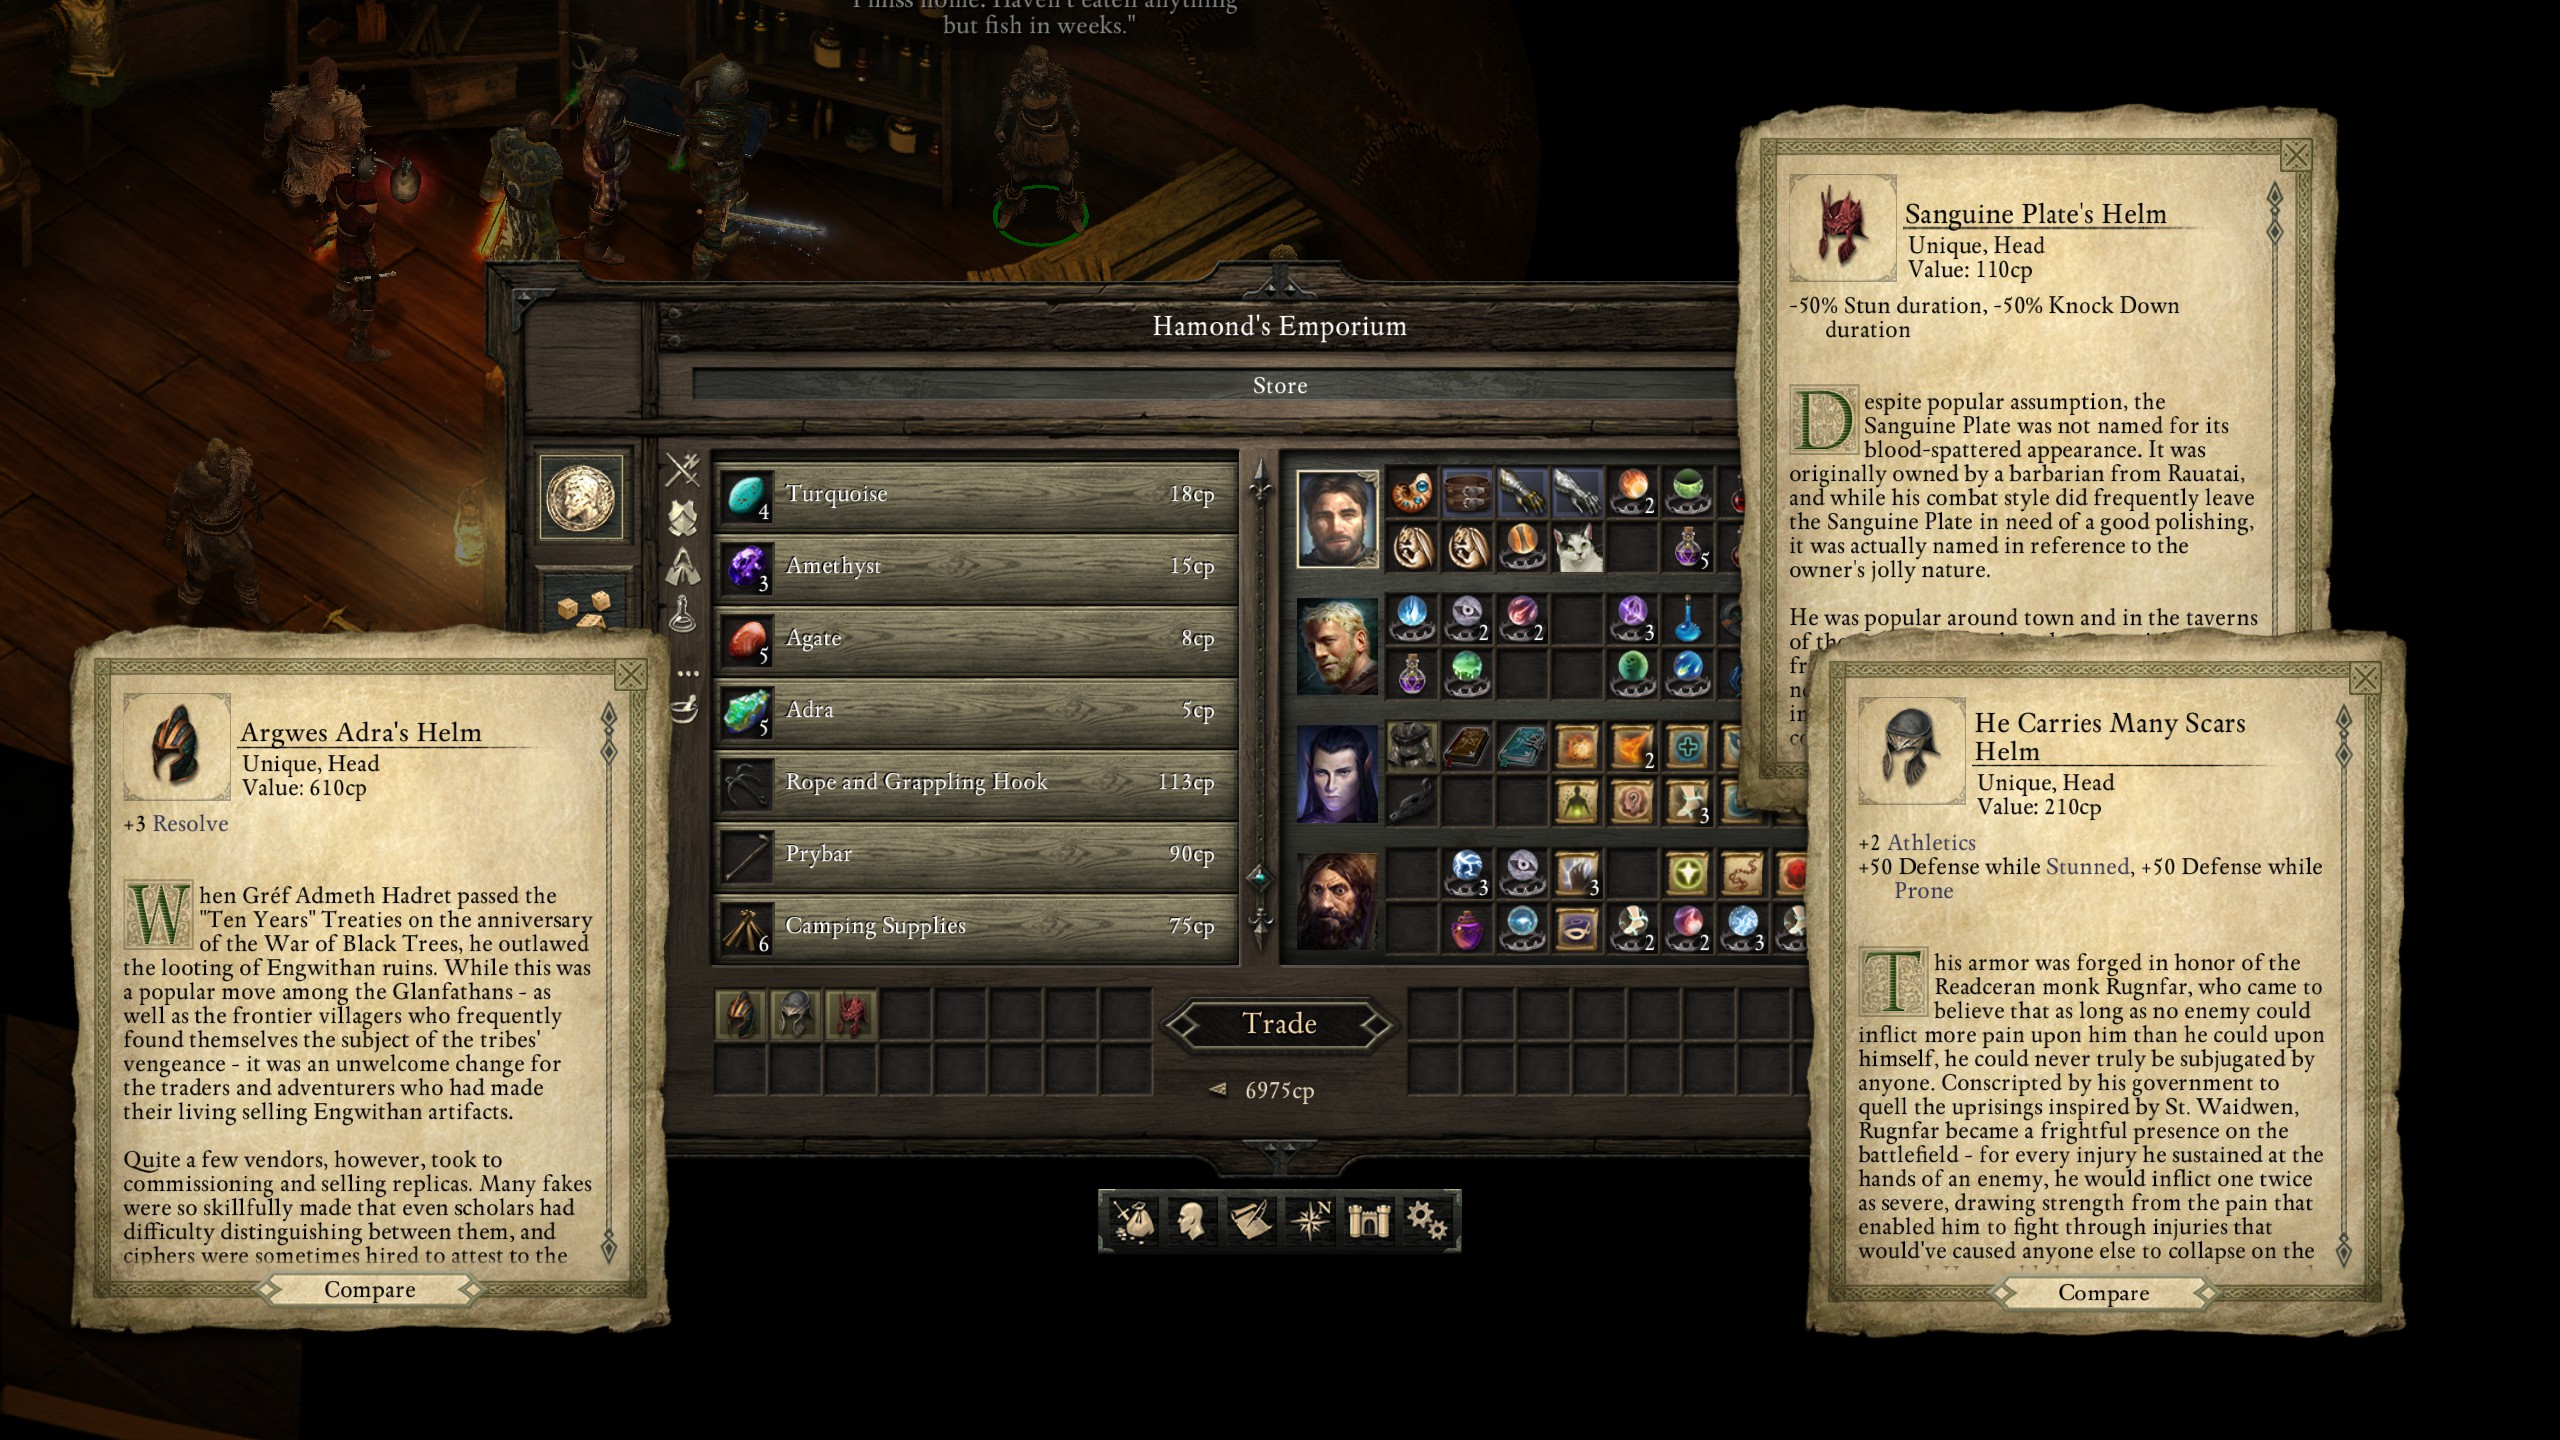
\includegraphics[scale=0.33]{files/blog/2020_01_18_poe_potd_wmpt2/2020_01_18_emporium.jpg}
\end{figure}

After purchasing and equipping the helmets I then travelled into the mines.

\begin{figure}
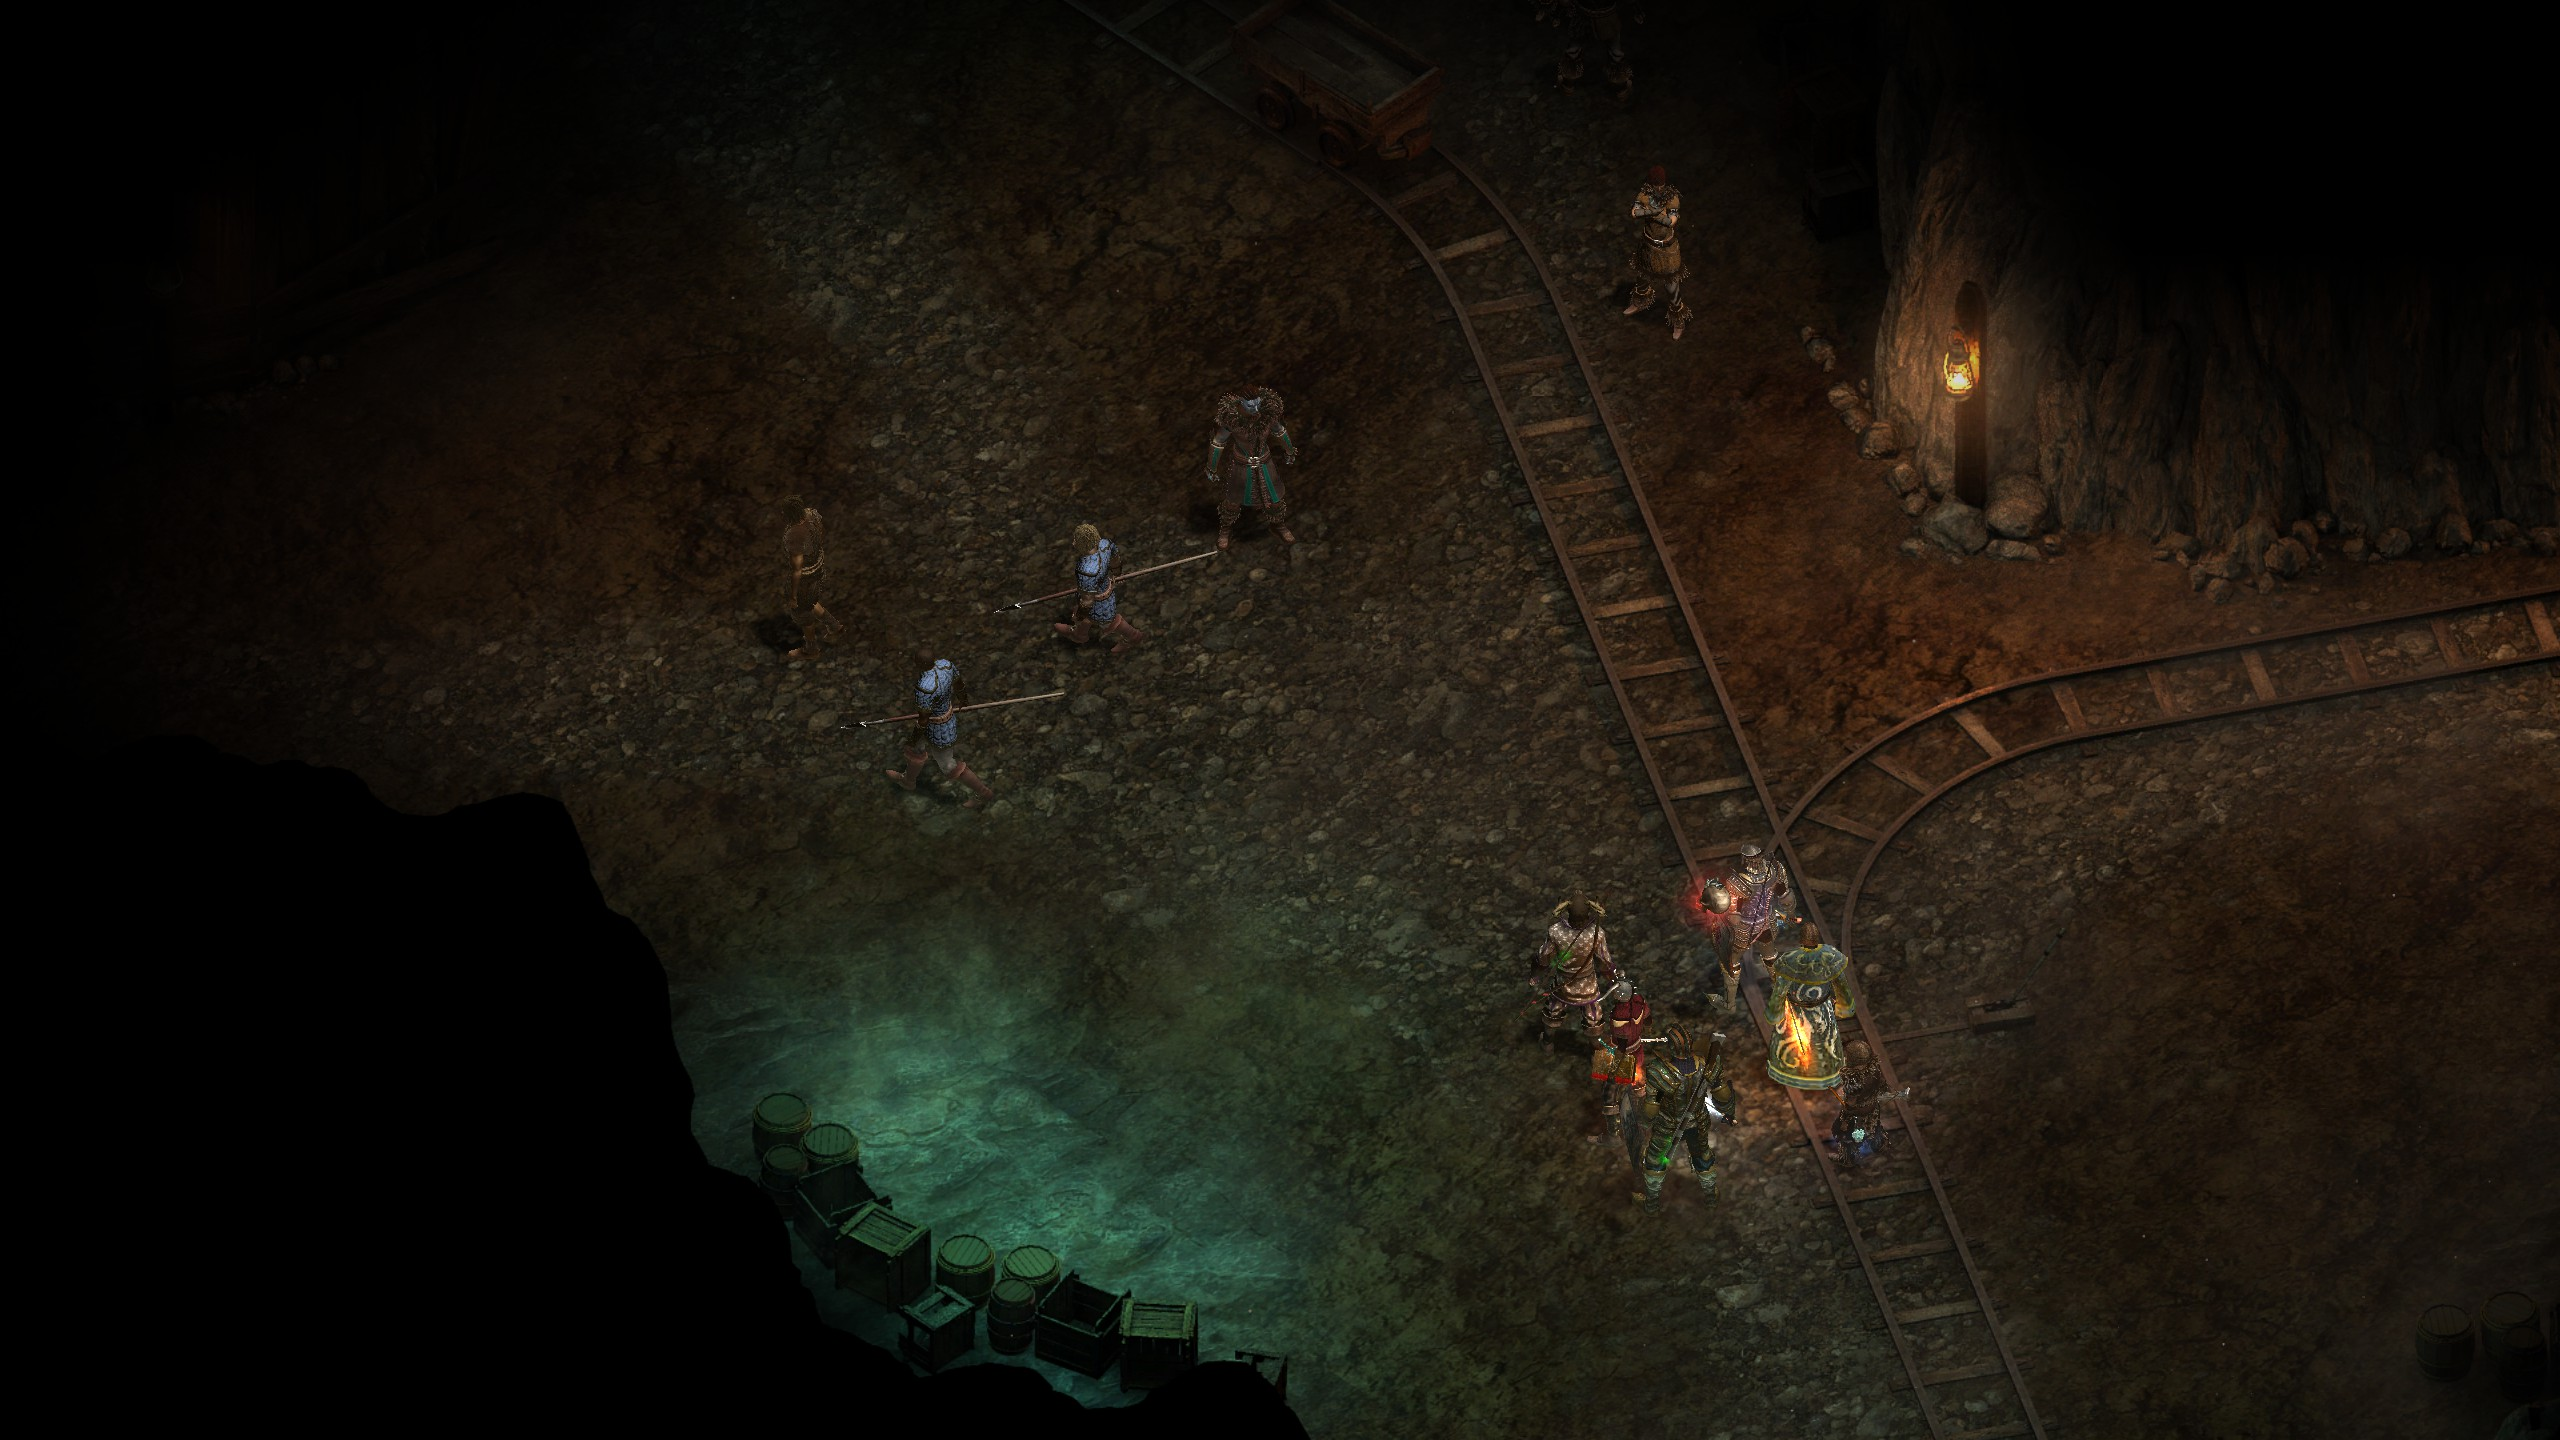
\includegraphics[scale=0.33]{files/blog/2020_01_18_poe_potd_wmpt2/2020_01_18_mines1.jpg}
\end{figure}

Though none of the fights had been particularly challenging thus far, the high difficulty (plus expert mode) meant that I had to watch my health closely; I made the mistake of pushing too hard and got close to actually dying, though ``Barring Death's Door'' would have protected me for another 5 seconds.

\begin{figure}
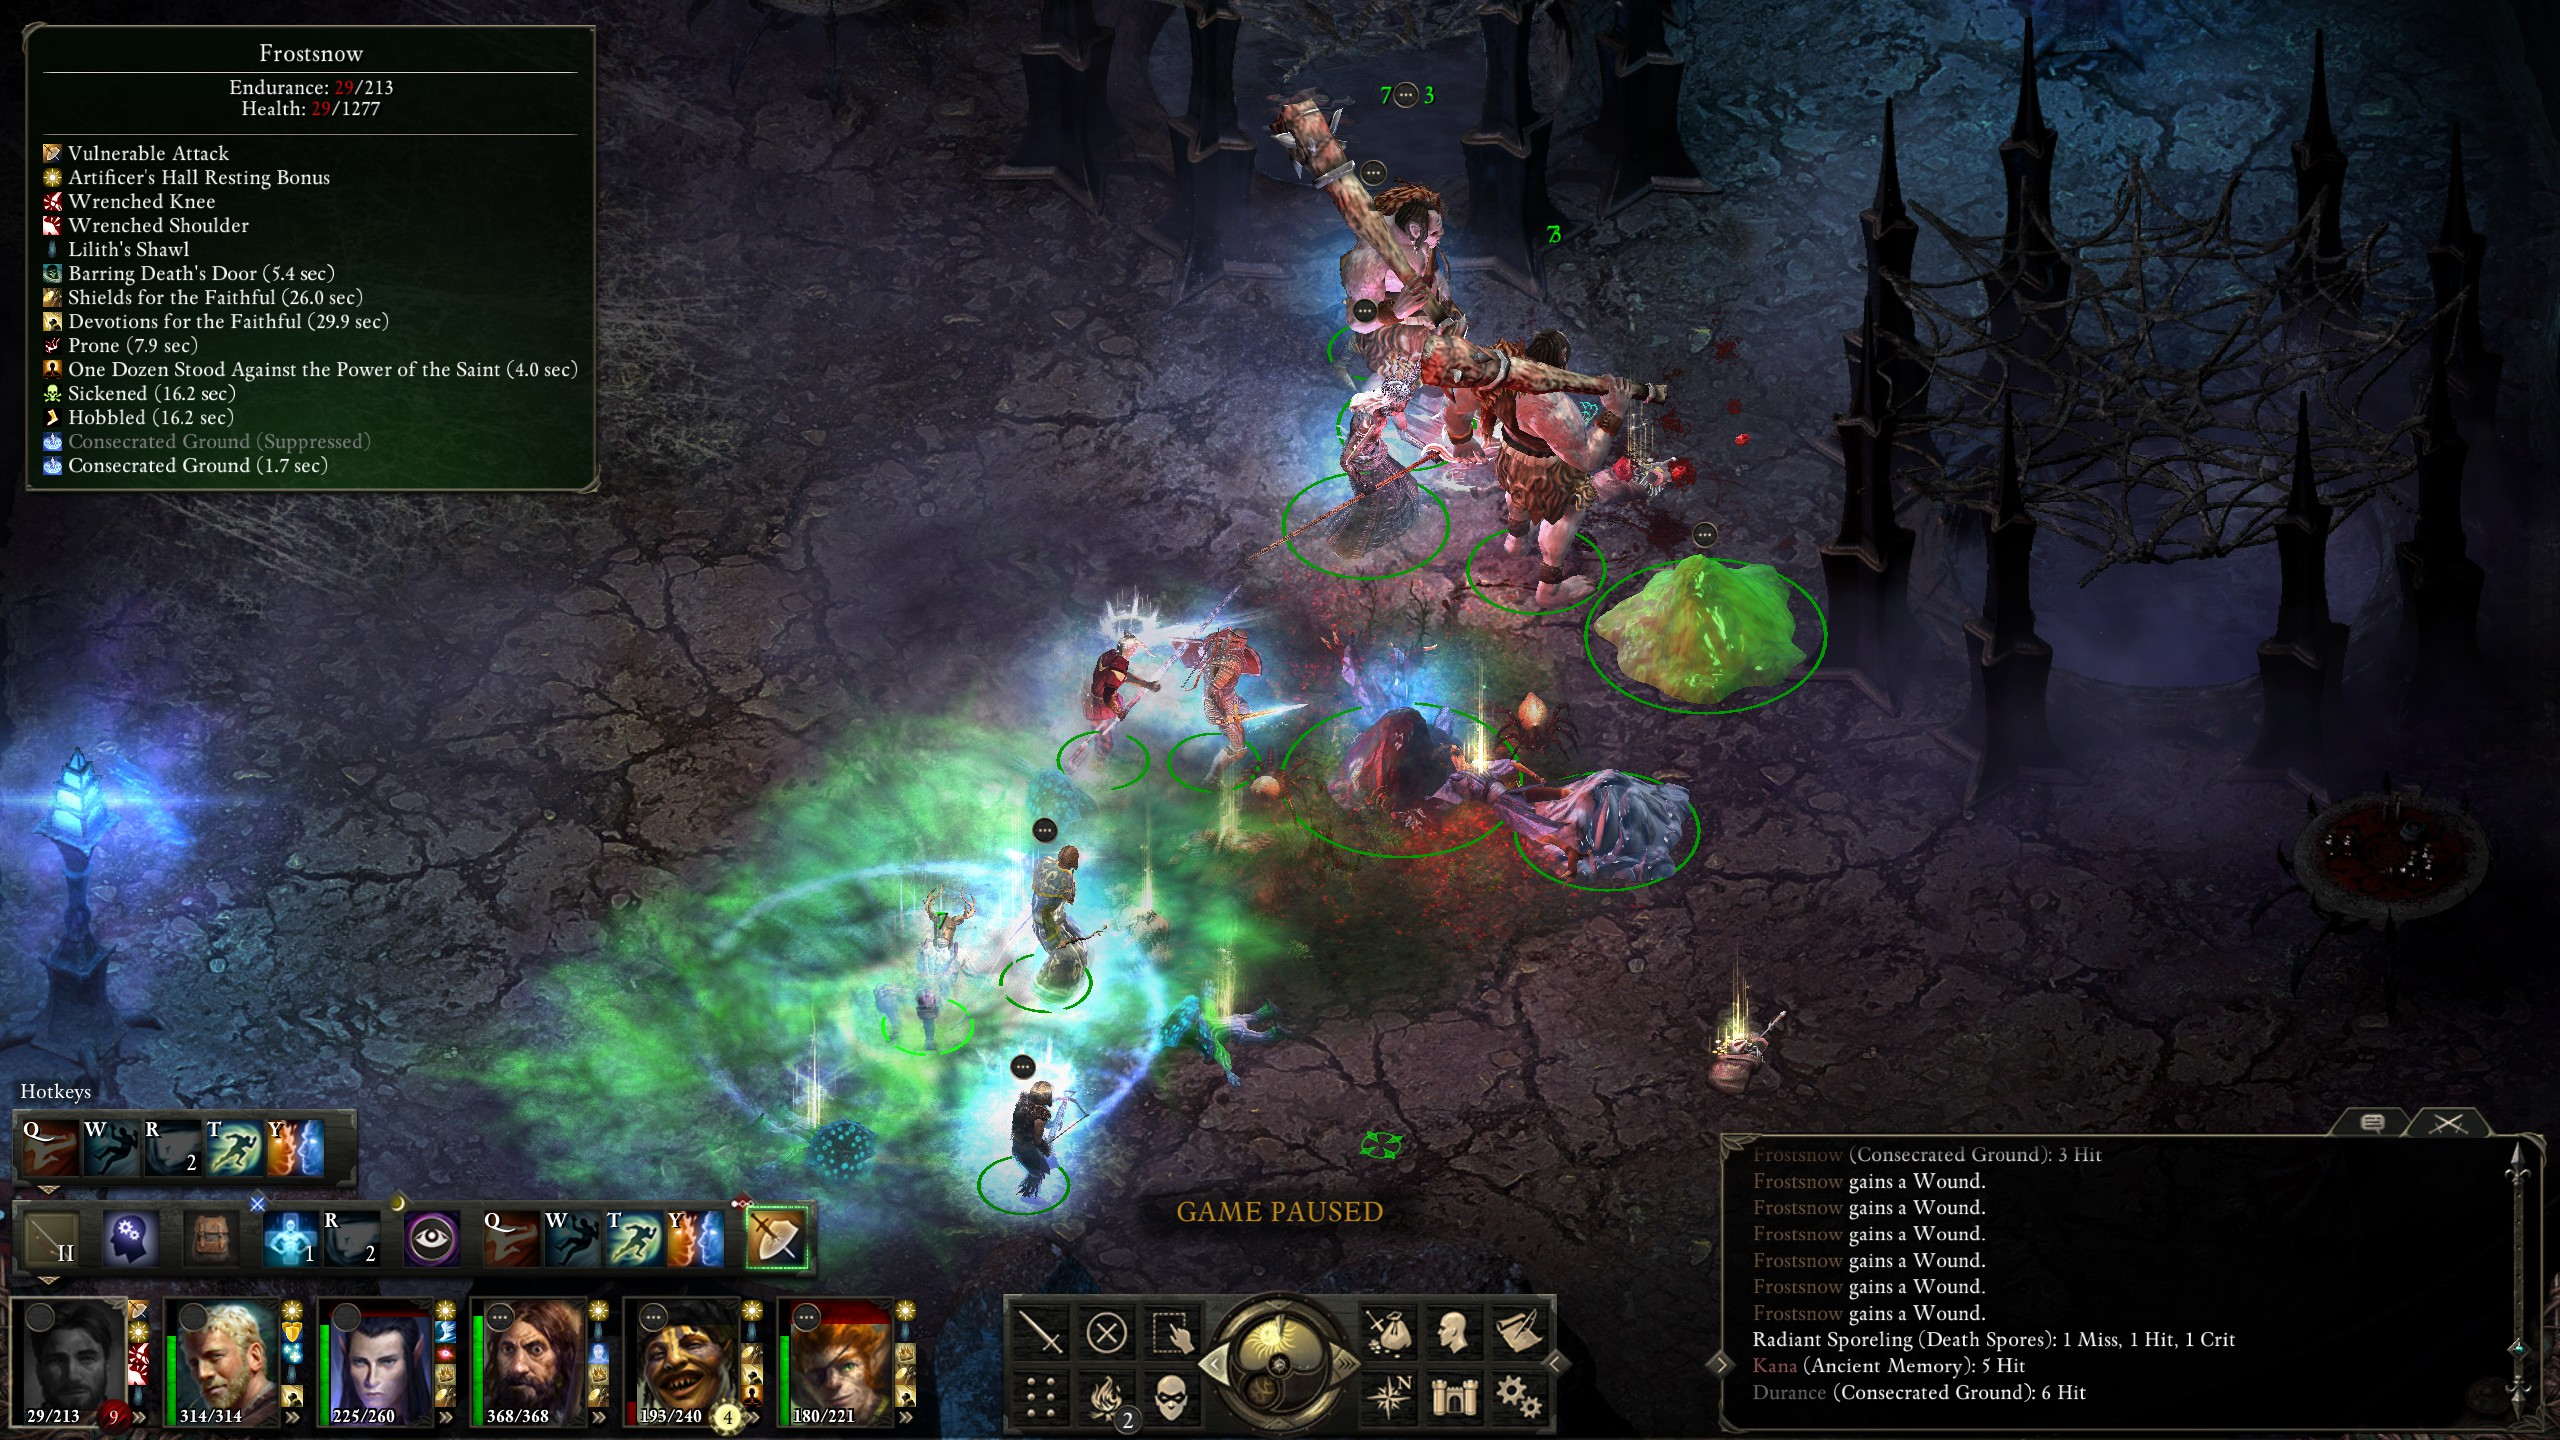
\includegraphics[scale=0.33]{files/blog/2020_01_18_poe_potd_wmpt2/2020_01_18_mines2.jpg}
\end{figure}

Before long I made it to the vithrack colony, where the vithrack brutes gave me a hard time by going straight for my squishy monk.  It gave my monk plenty of wounds to retaliate with, though, when he wasn't being stun-locked.  In the meantime Durance had to use ``Prayer Against Treachery'' to prevent half of my team turning against itself.

\begin{figure}
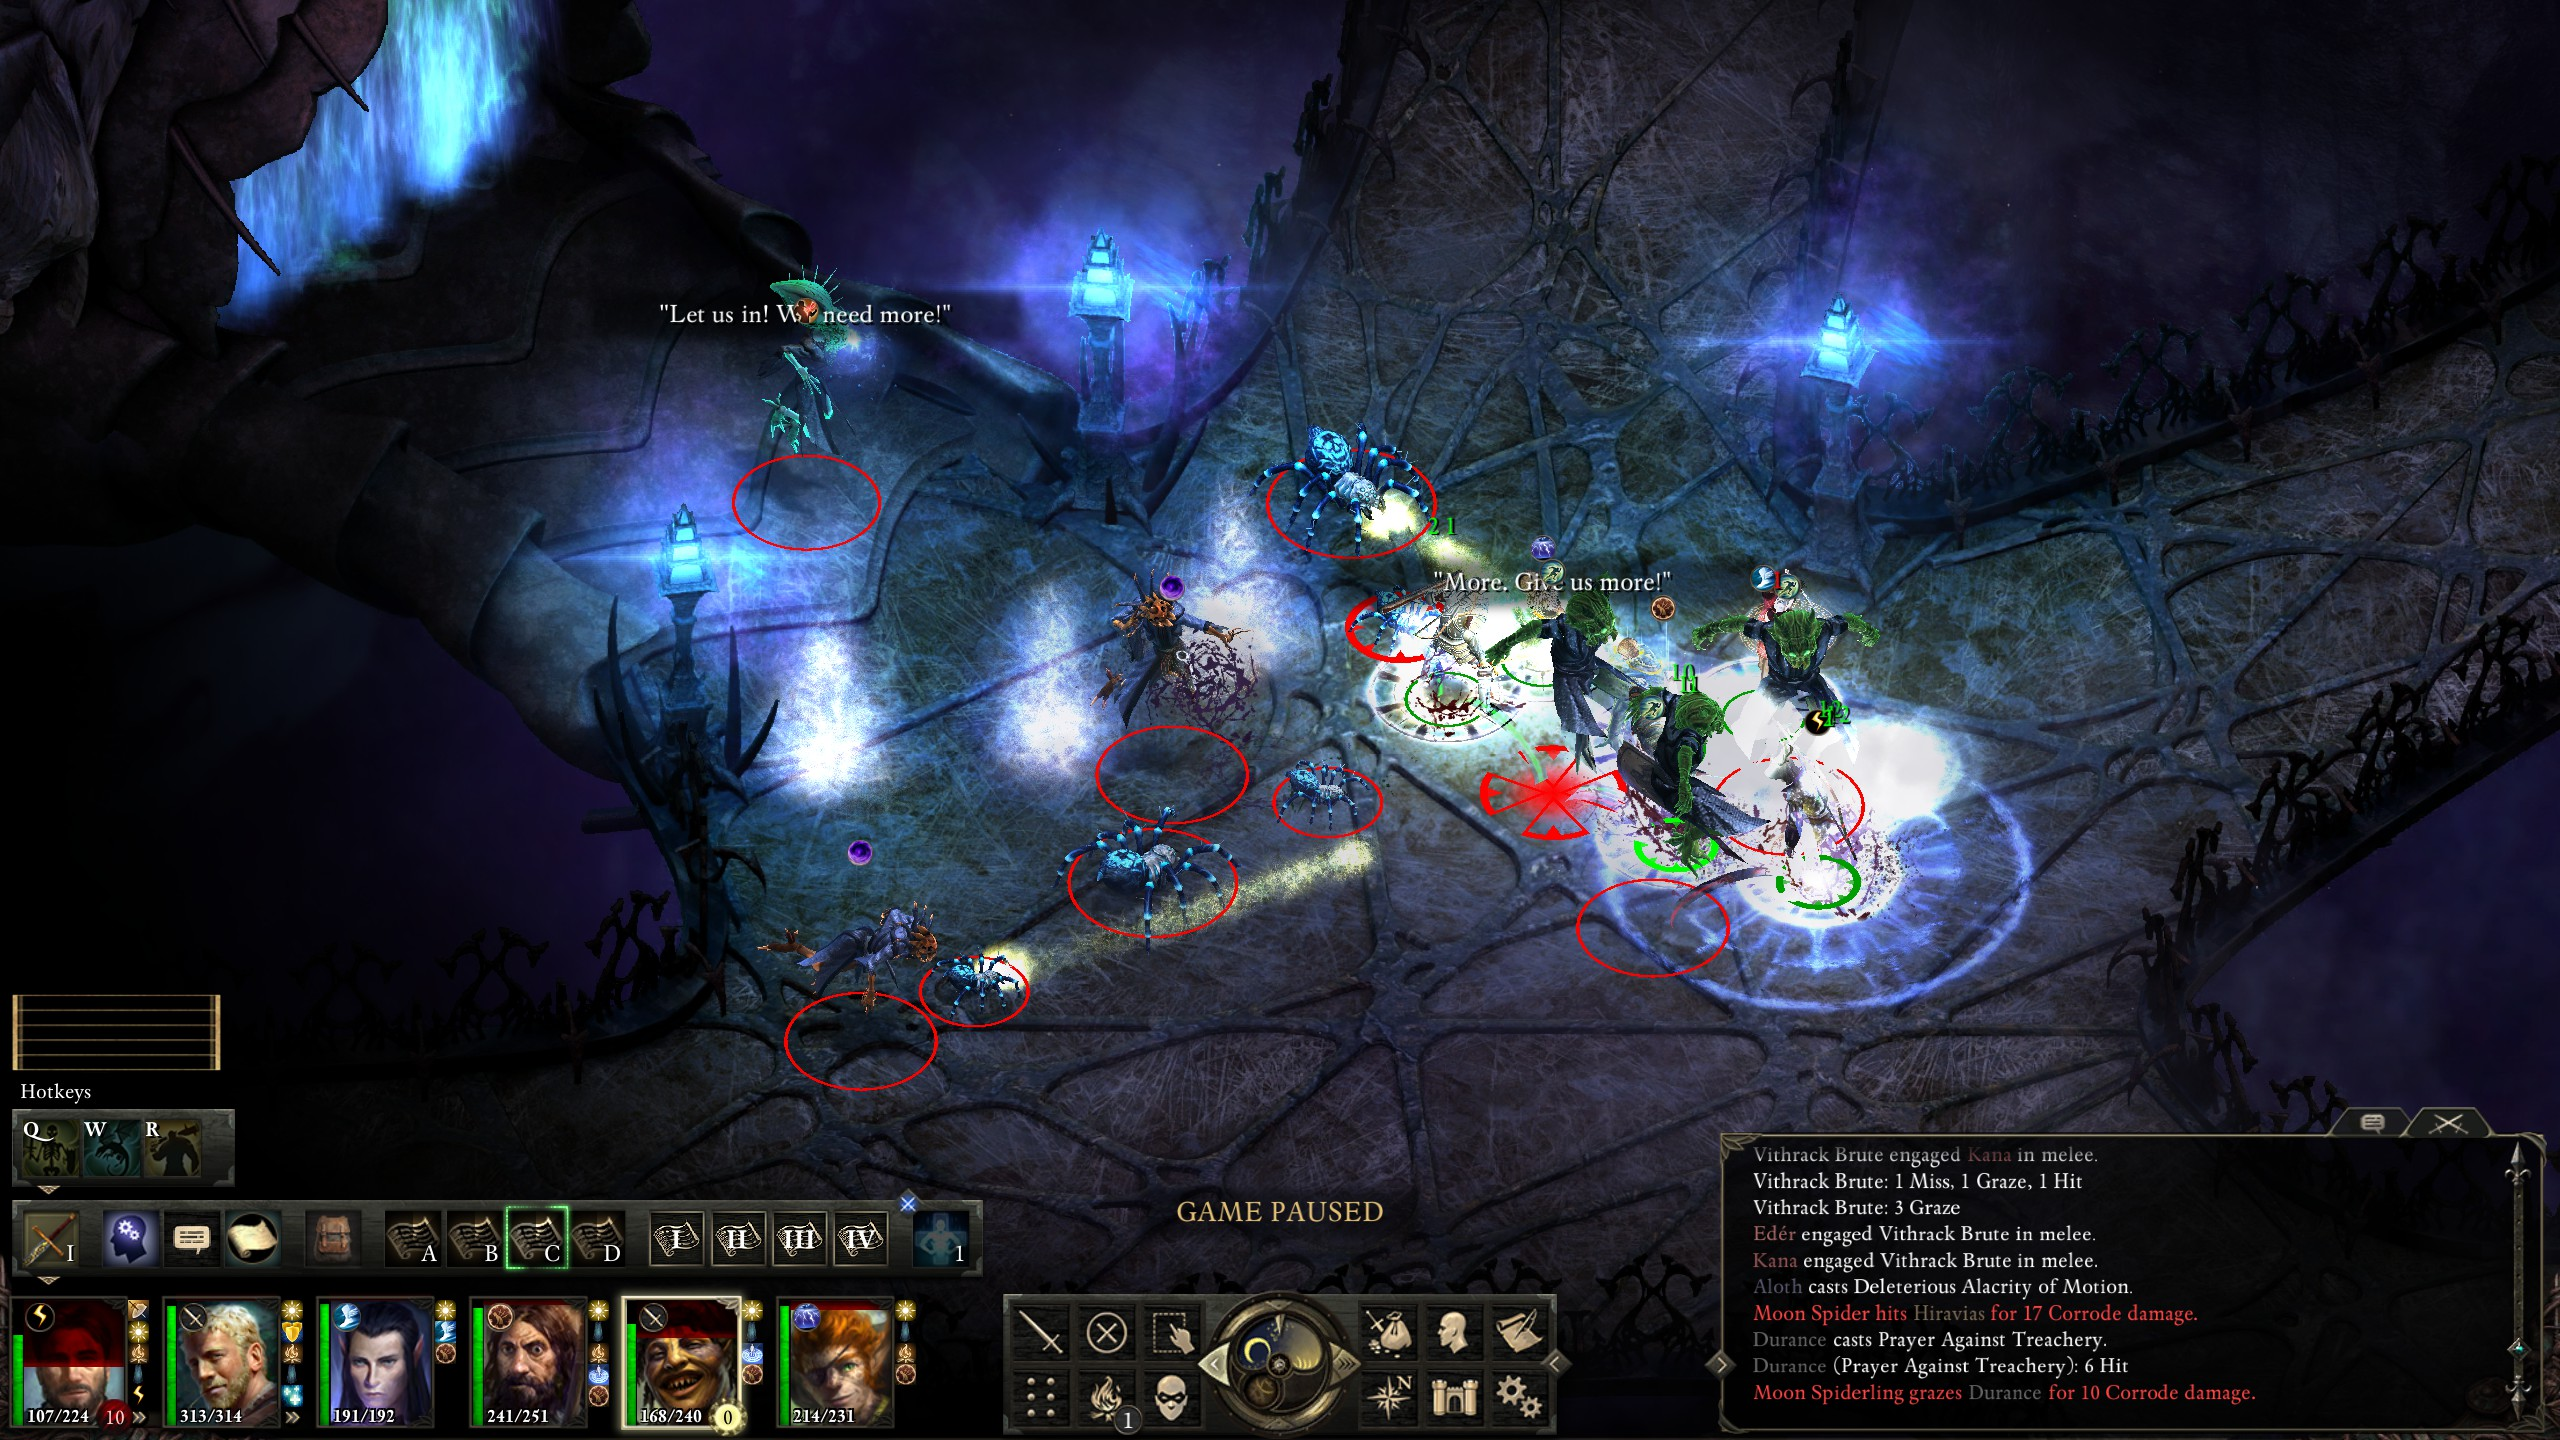
\includegraphics[scale=0.33]{files/blog/2020_01_18_poe_potd_wmpt2/2020_01_18_mines3.jpg}
\end{figure}

After battling through the chambers I finally made it into the giant spore boss in the commons.

\begin{figure}
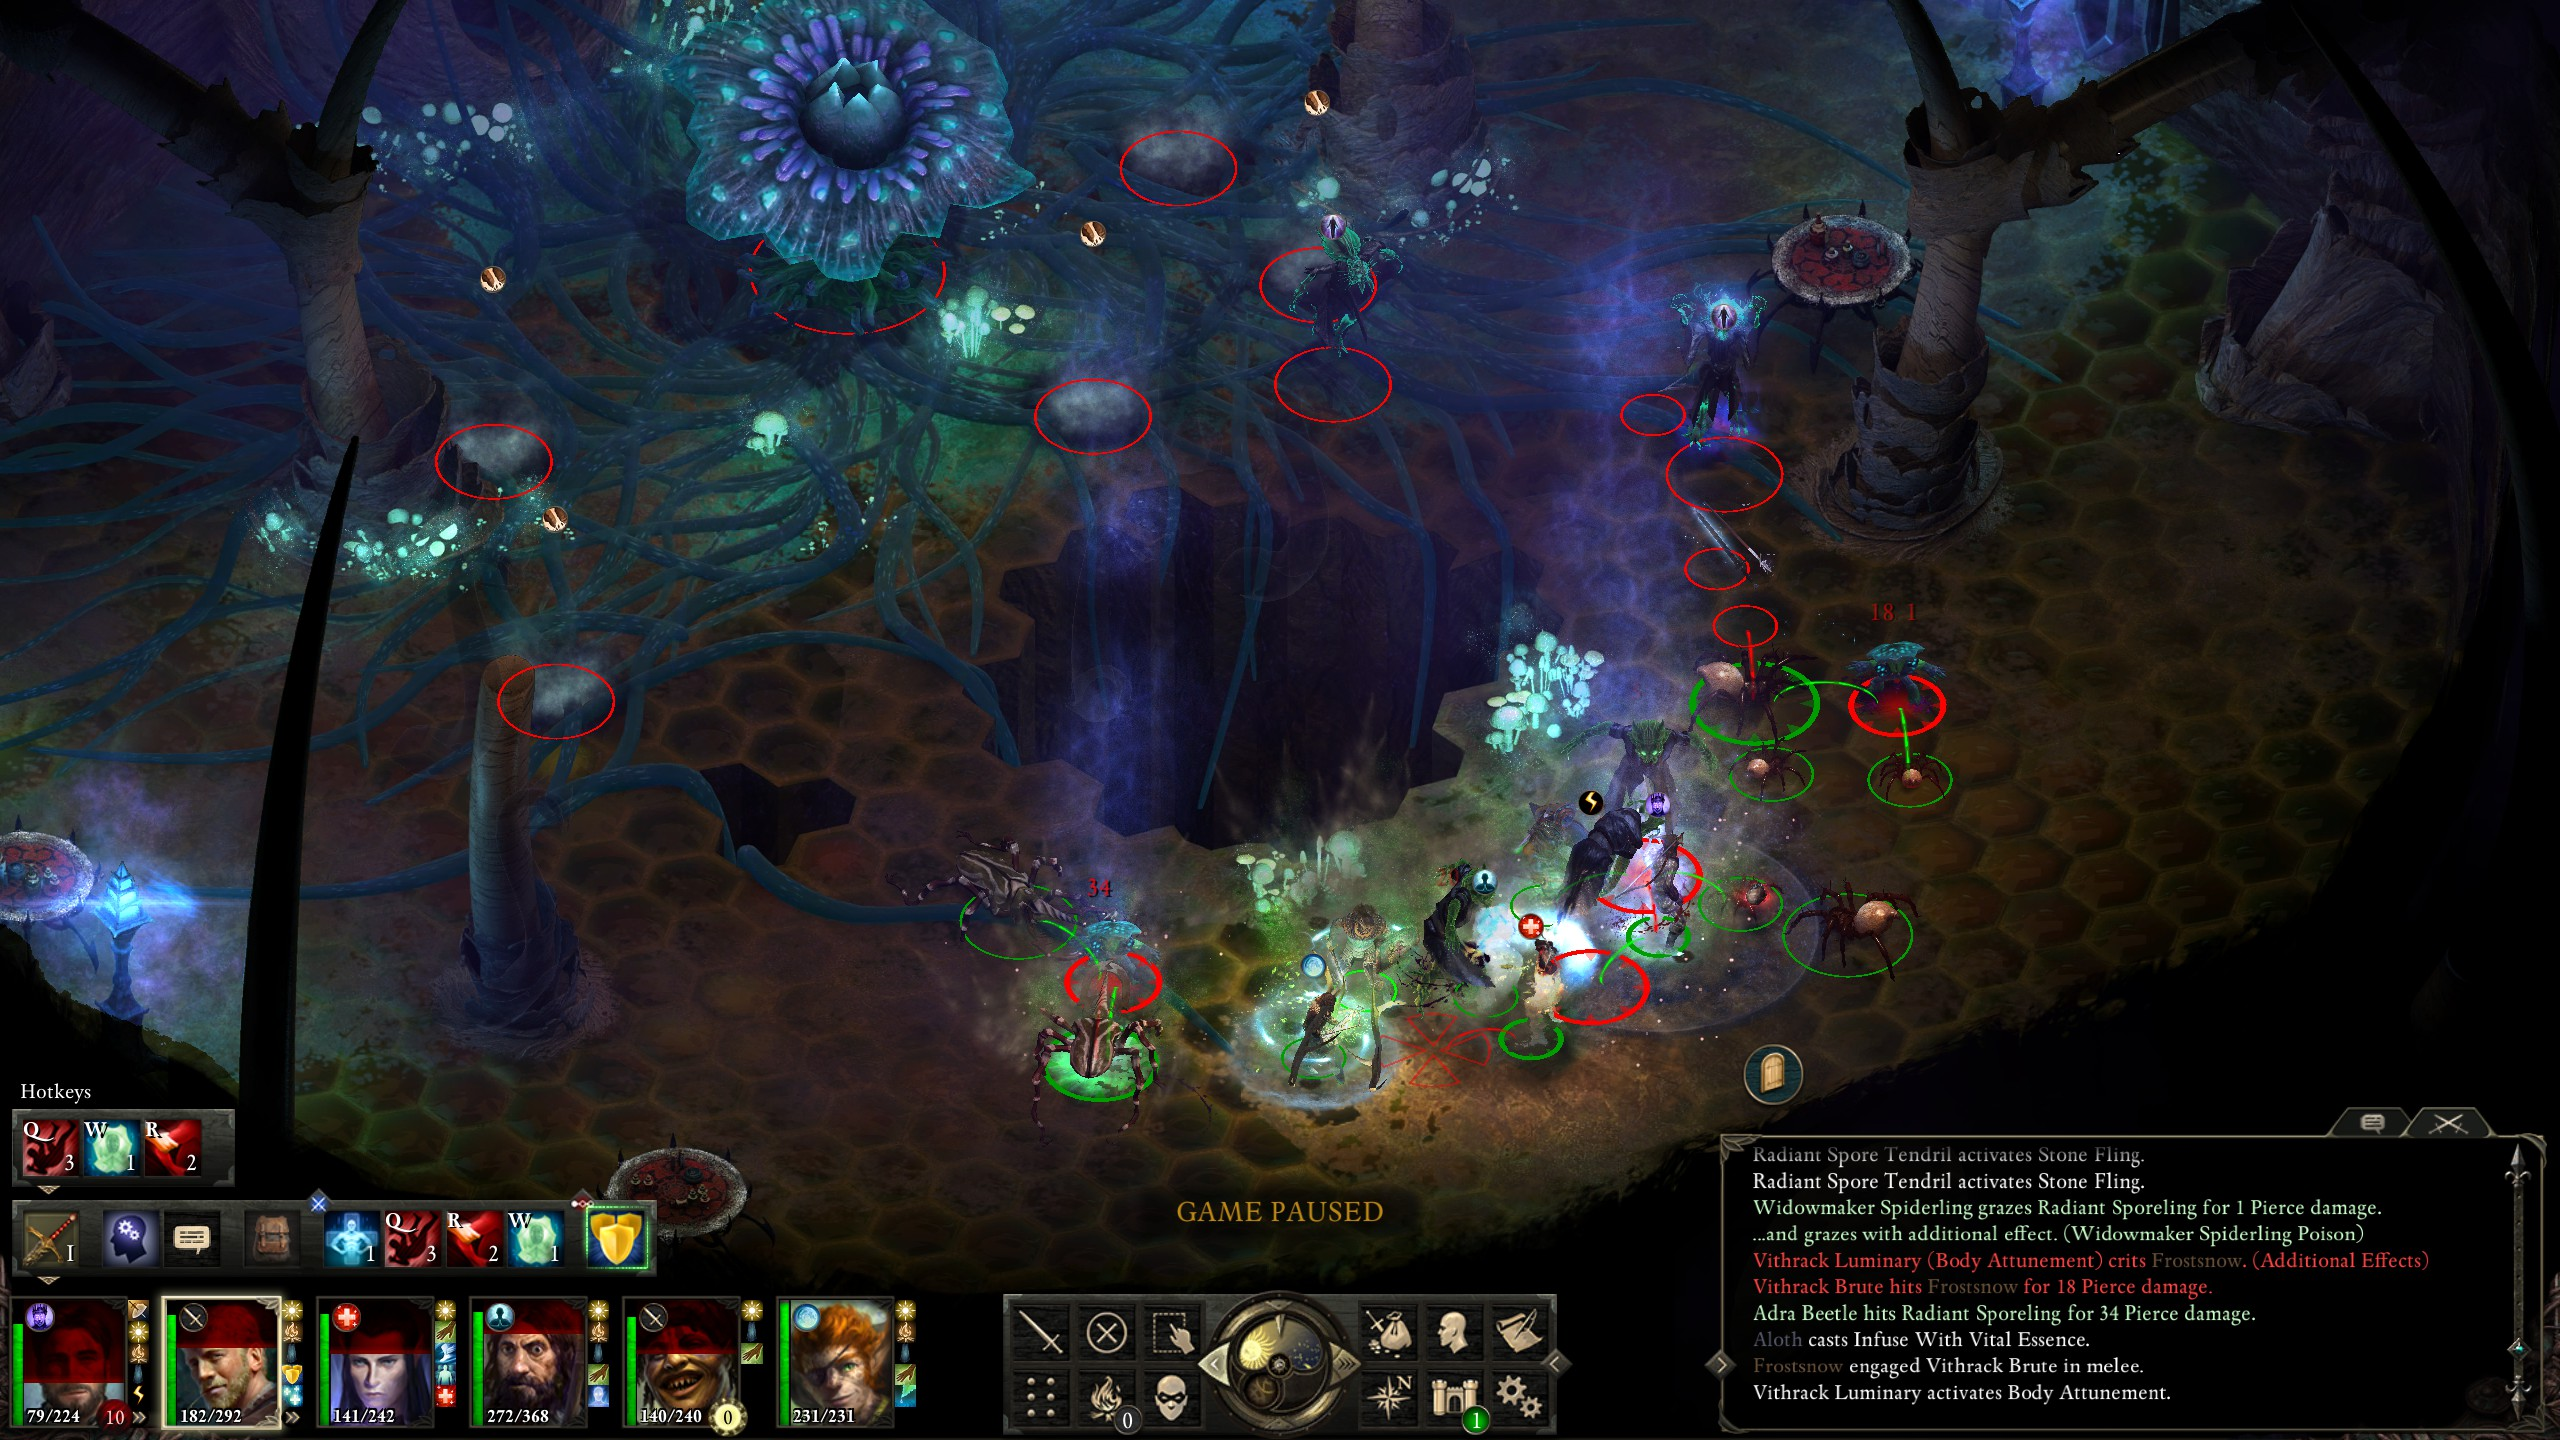
\includegraphics[scale=0.33]{files/blog/2020_01_18_poe_potd_wmpt2/2020_01_18_mines4.jpg}
\end{figure}

Like the vithrack brutes from earlier, the boss intelligently had all of its tentacles sling rocks at the same, weak target.  Unintelligently, though, the boss attacked the temporary allies that I summoned with trinkets, leaving my monk free to deal massive damage.

\begin{figure}
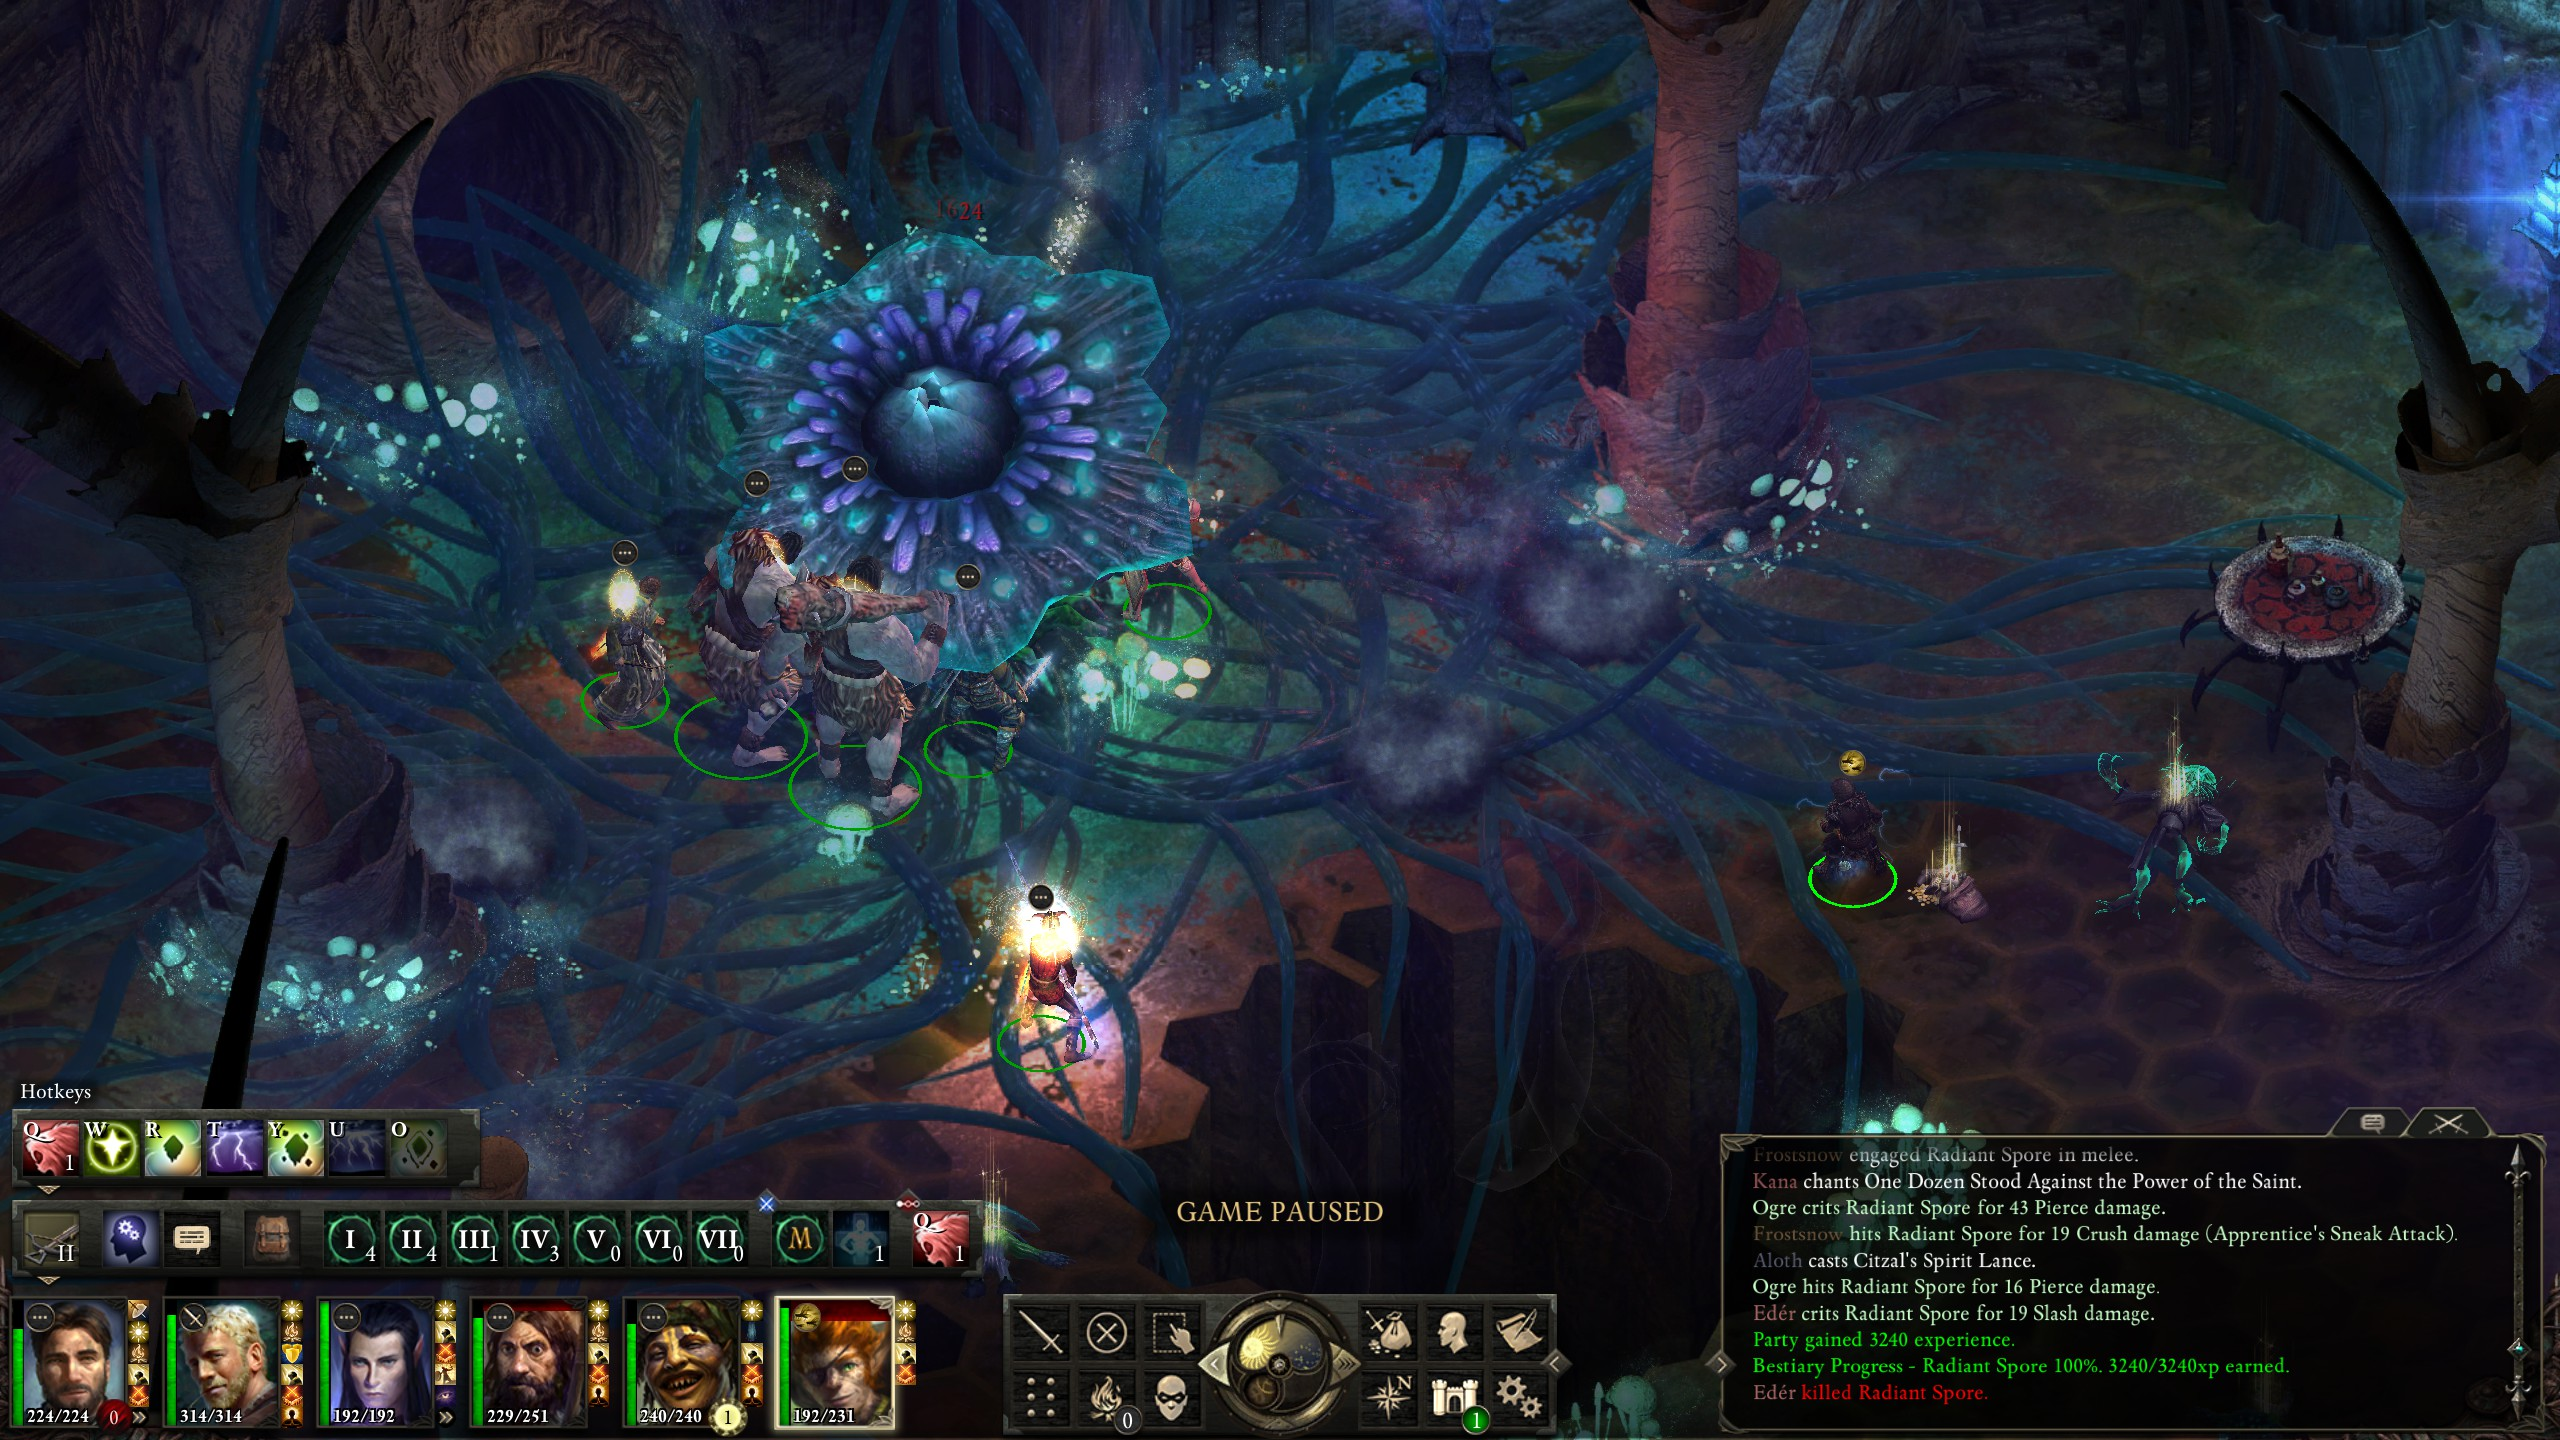
\includegraphics[scale=0.33]{files/blog/2020_01_18_poe_potd_wmpt2/2020_01_18_mines5.jpg}
\end{figure}

I thus slowly pushed my way through the adds and took out the boss without much trouble.  With the mines cleared, I then headed to Durgan's Battery in order to clear out the cannon tower.

\subsection{Durgan's Battery West Tower}
The monsters in the tower did not present much of a problem, except perhaps the Forge Guardians, but Hiravias' ``Weather the Storm Spell'' neutralized much of their potential damage.

\begin{figure}
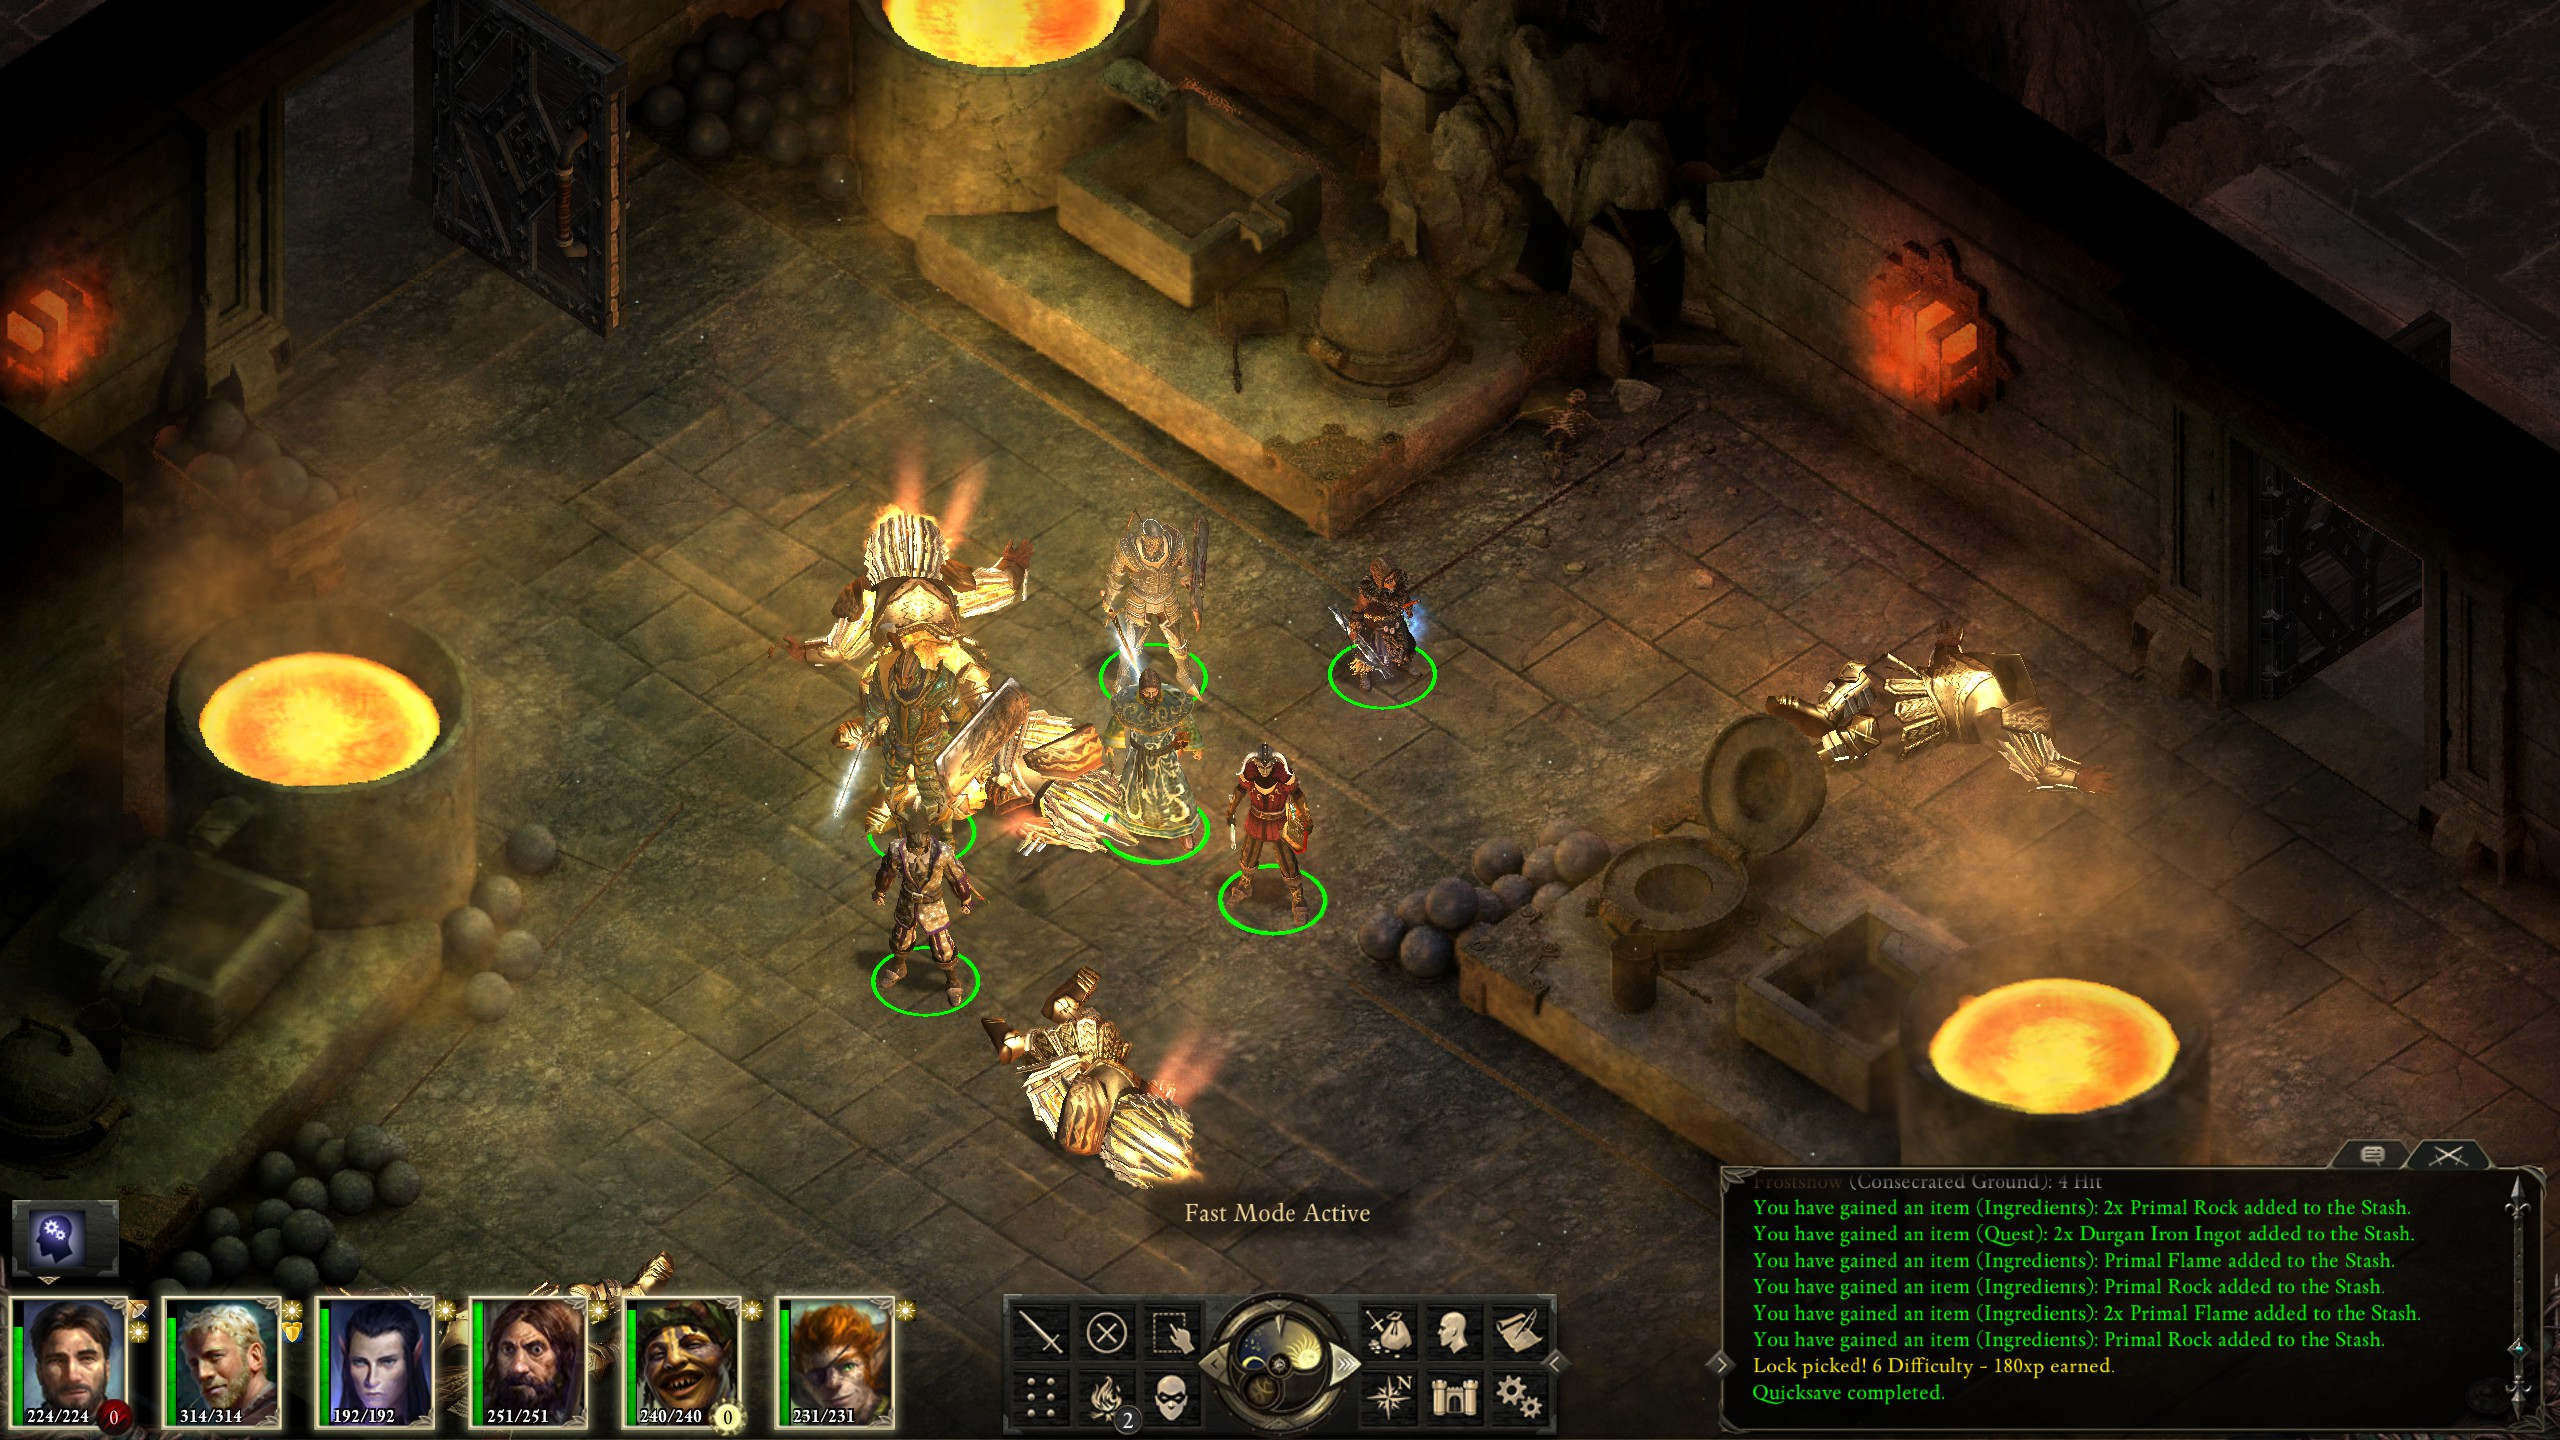
\includegraphics[scale=0.33]{files/blog/2020_01_18_poe_potd_wmpt2/2020_01_18_tower1.jpg}
\end{figure}

After clearing the first floor I then gathered the items to repair the elevator and headed towards the cannons up top.

\begin{figure}
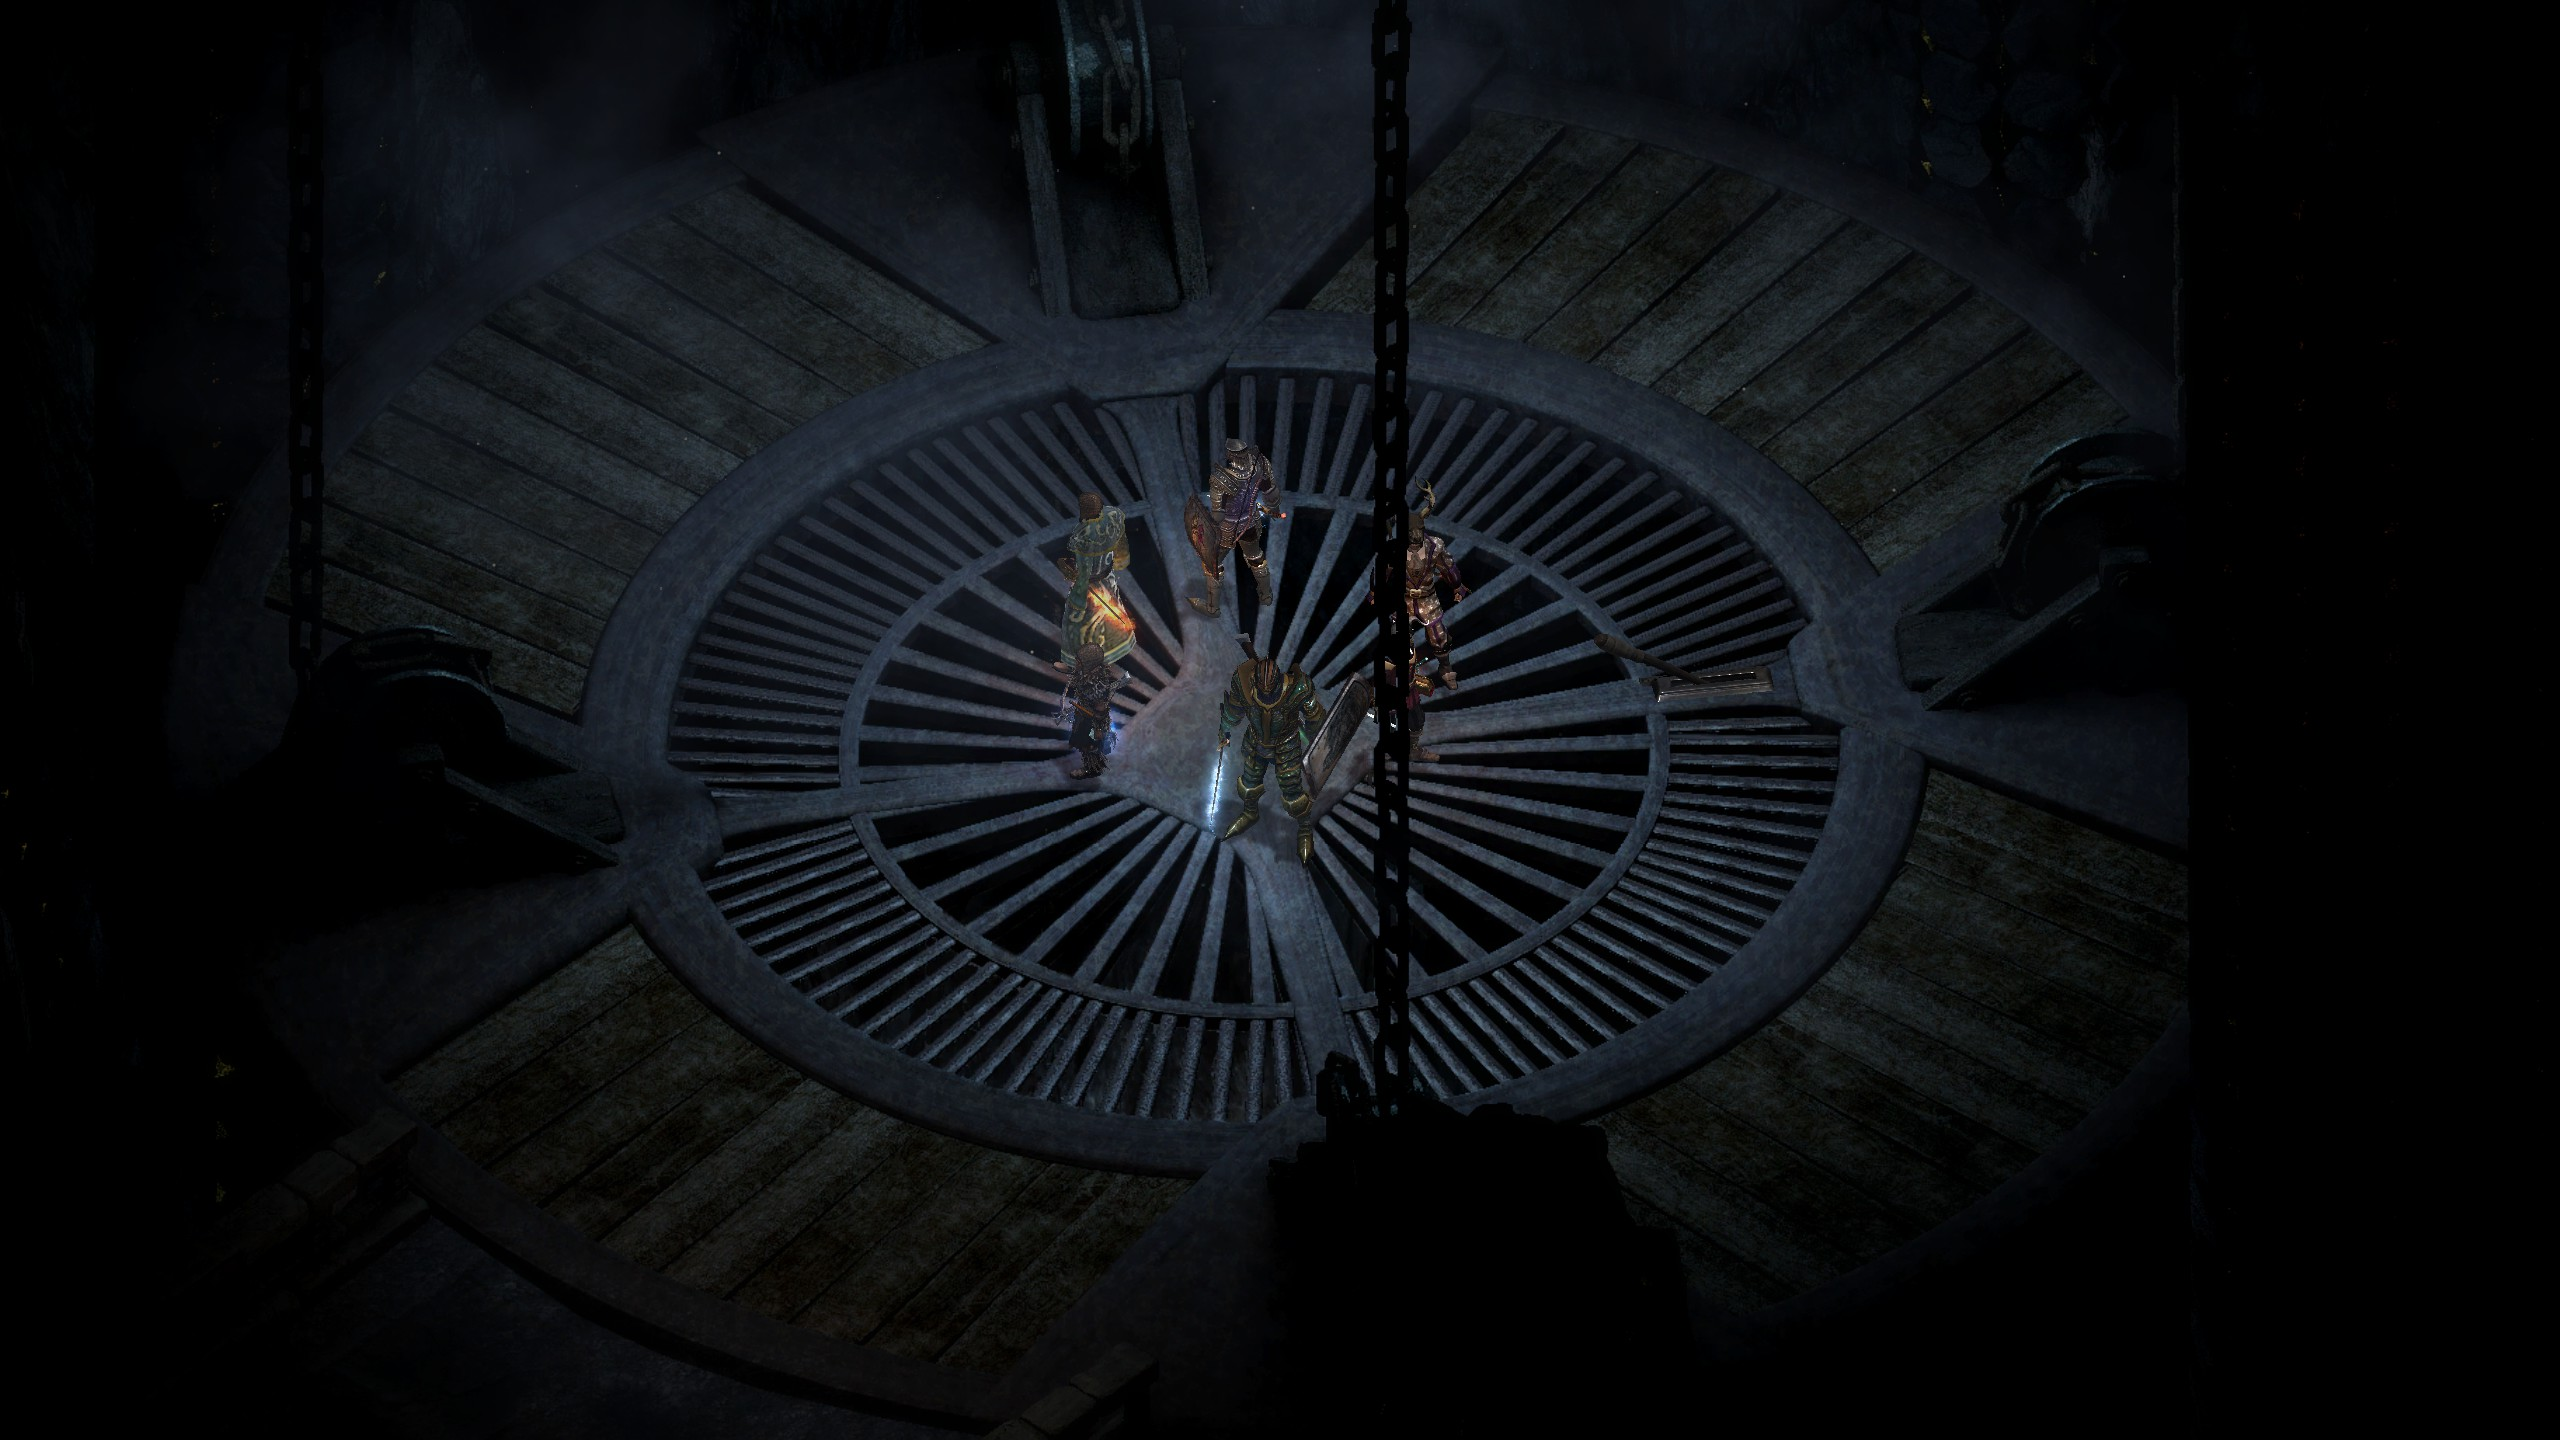
\includegraphics[scale=0.33]{files/blog/2020_01_18_poe_potd_wmpt2/2020_01_18_tower2.jpg}
\end{figure}

Once up top I cleared out the skuldrak and thawed out the cannons.

\begin{figure}
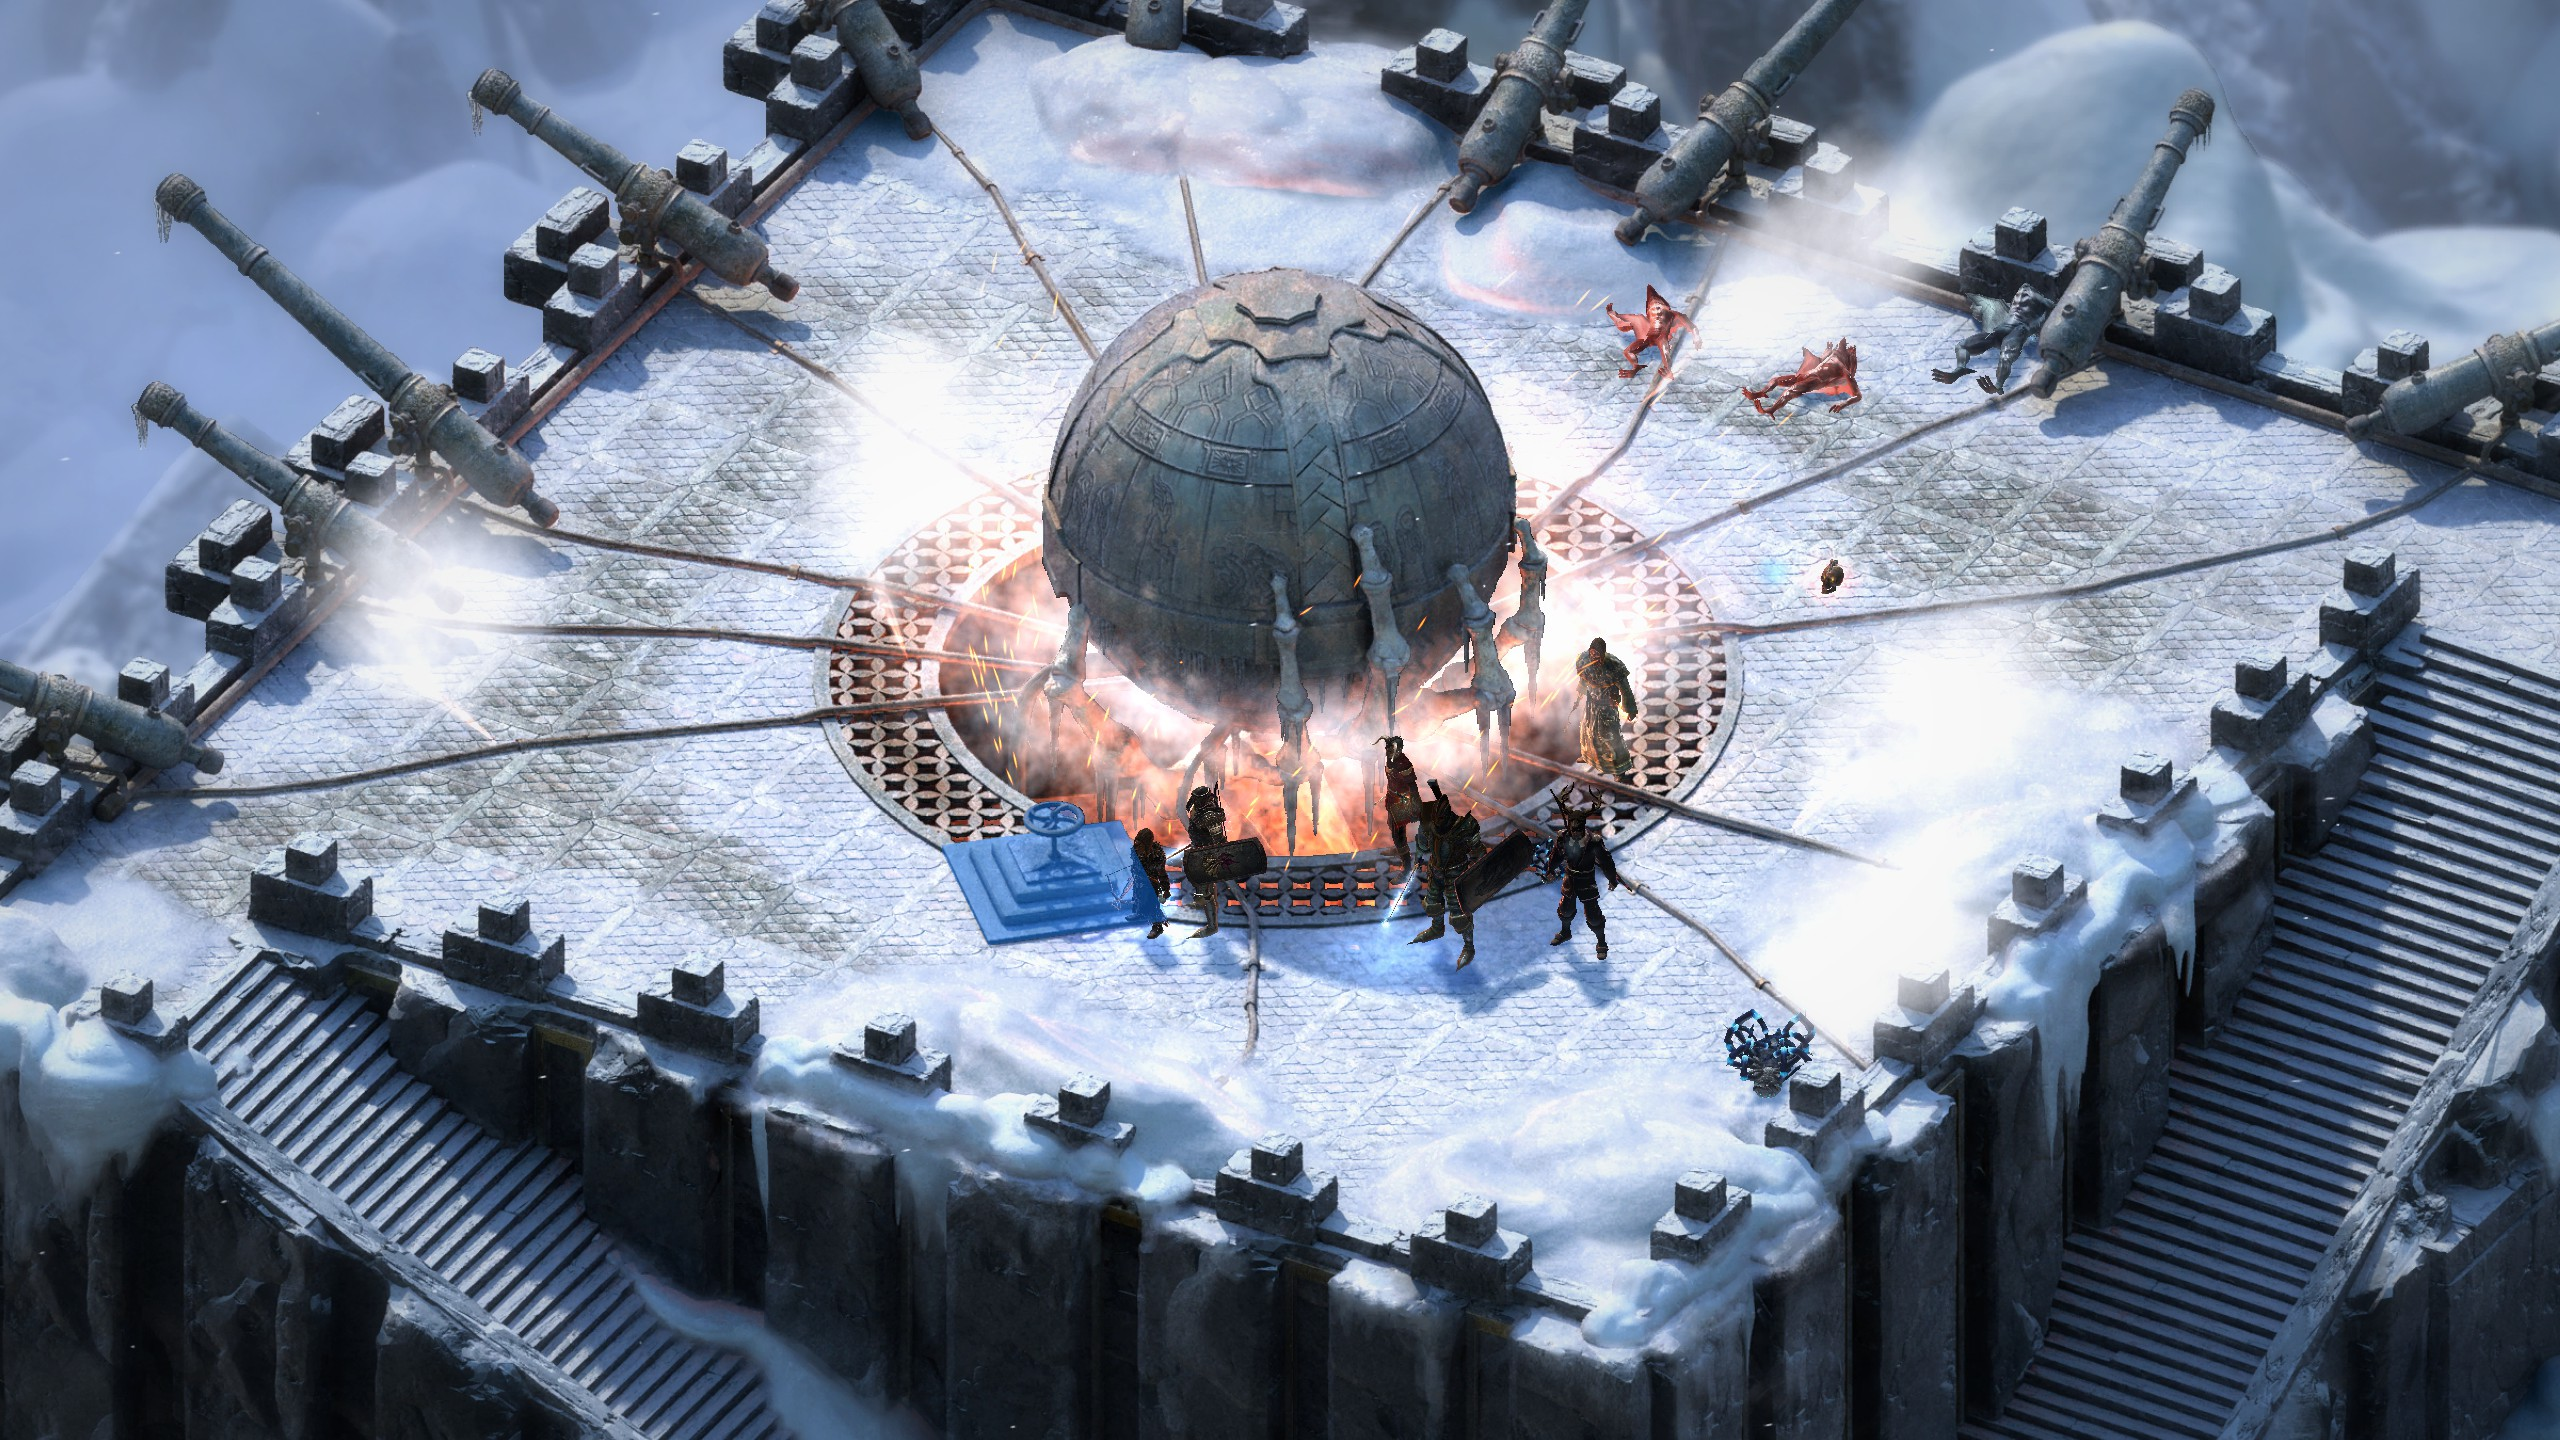
\includegraphics[scale=0.33]{files/blog/2020_01_18_poe_potd_wmpt2/2020_01_18_tower3.jpg}
\end{figure}

Easy enough, and the work would prove valuable later when I went to Iron Flail Fort.  Before that, though, I wanted to run the last of the bounty quests and also clear out the new wilderness area.

\subsection{Bounties and Whitestone Hollow}
First on the bounty list were the Redwater Lagufaeth; a small army of lagufaeth.

\begin{figure}
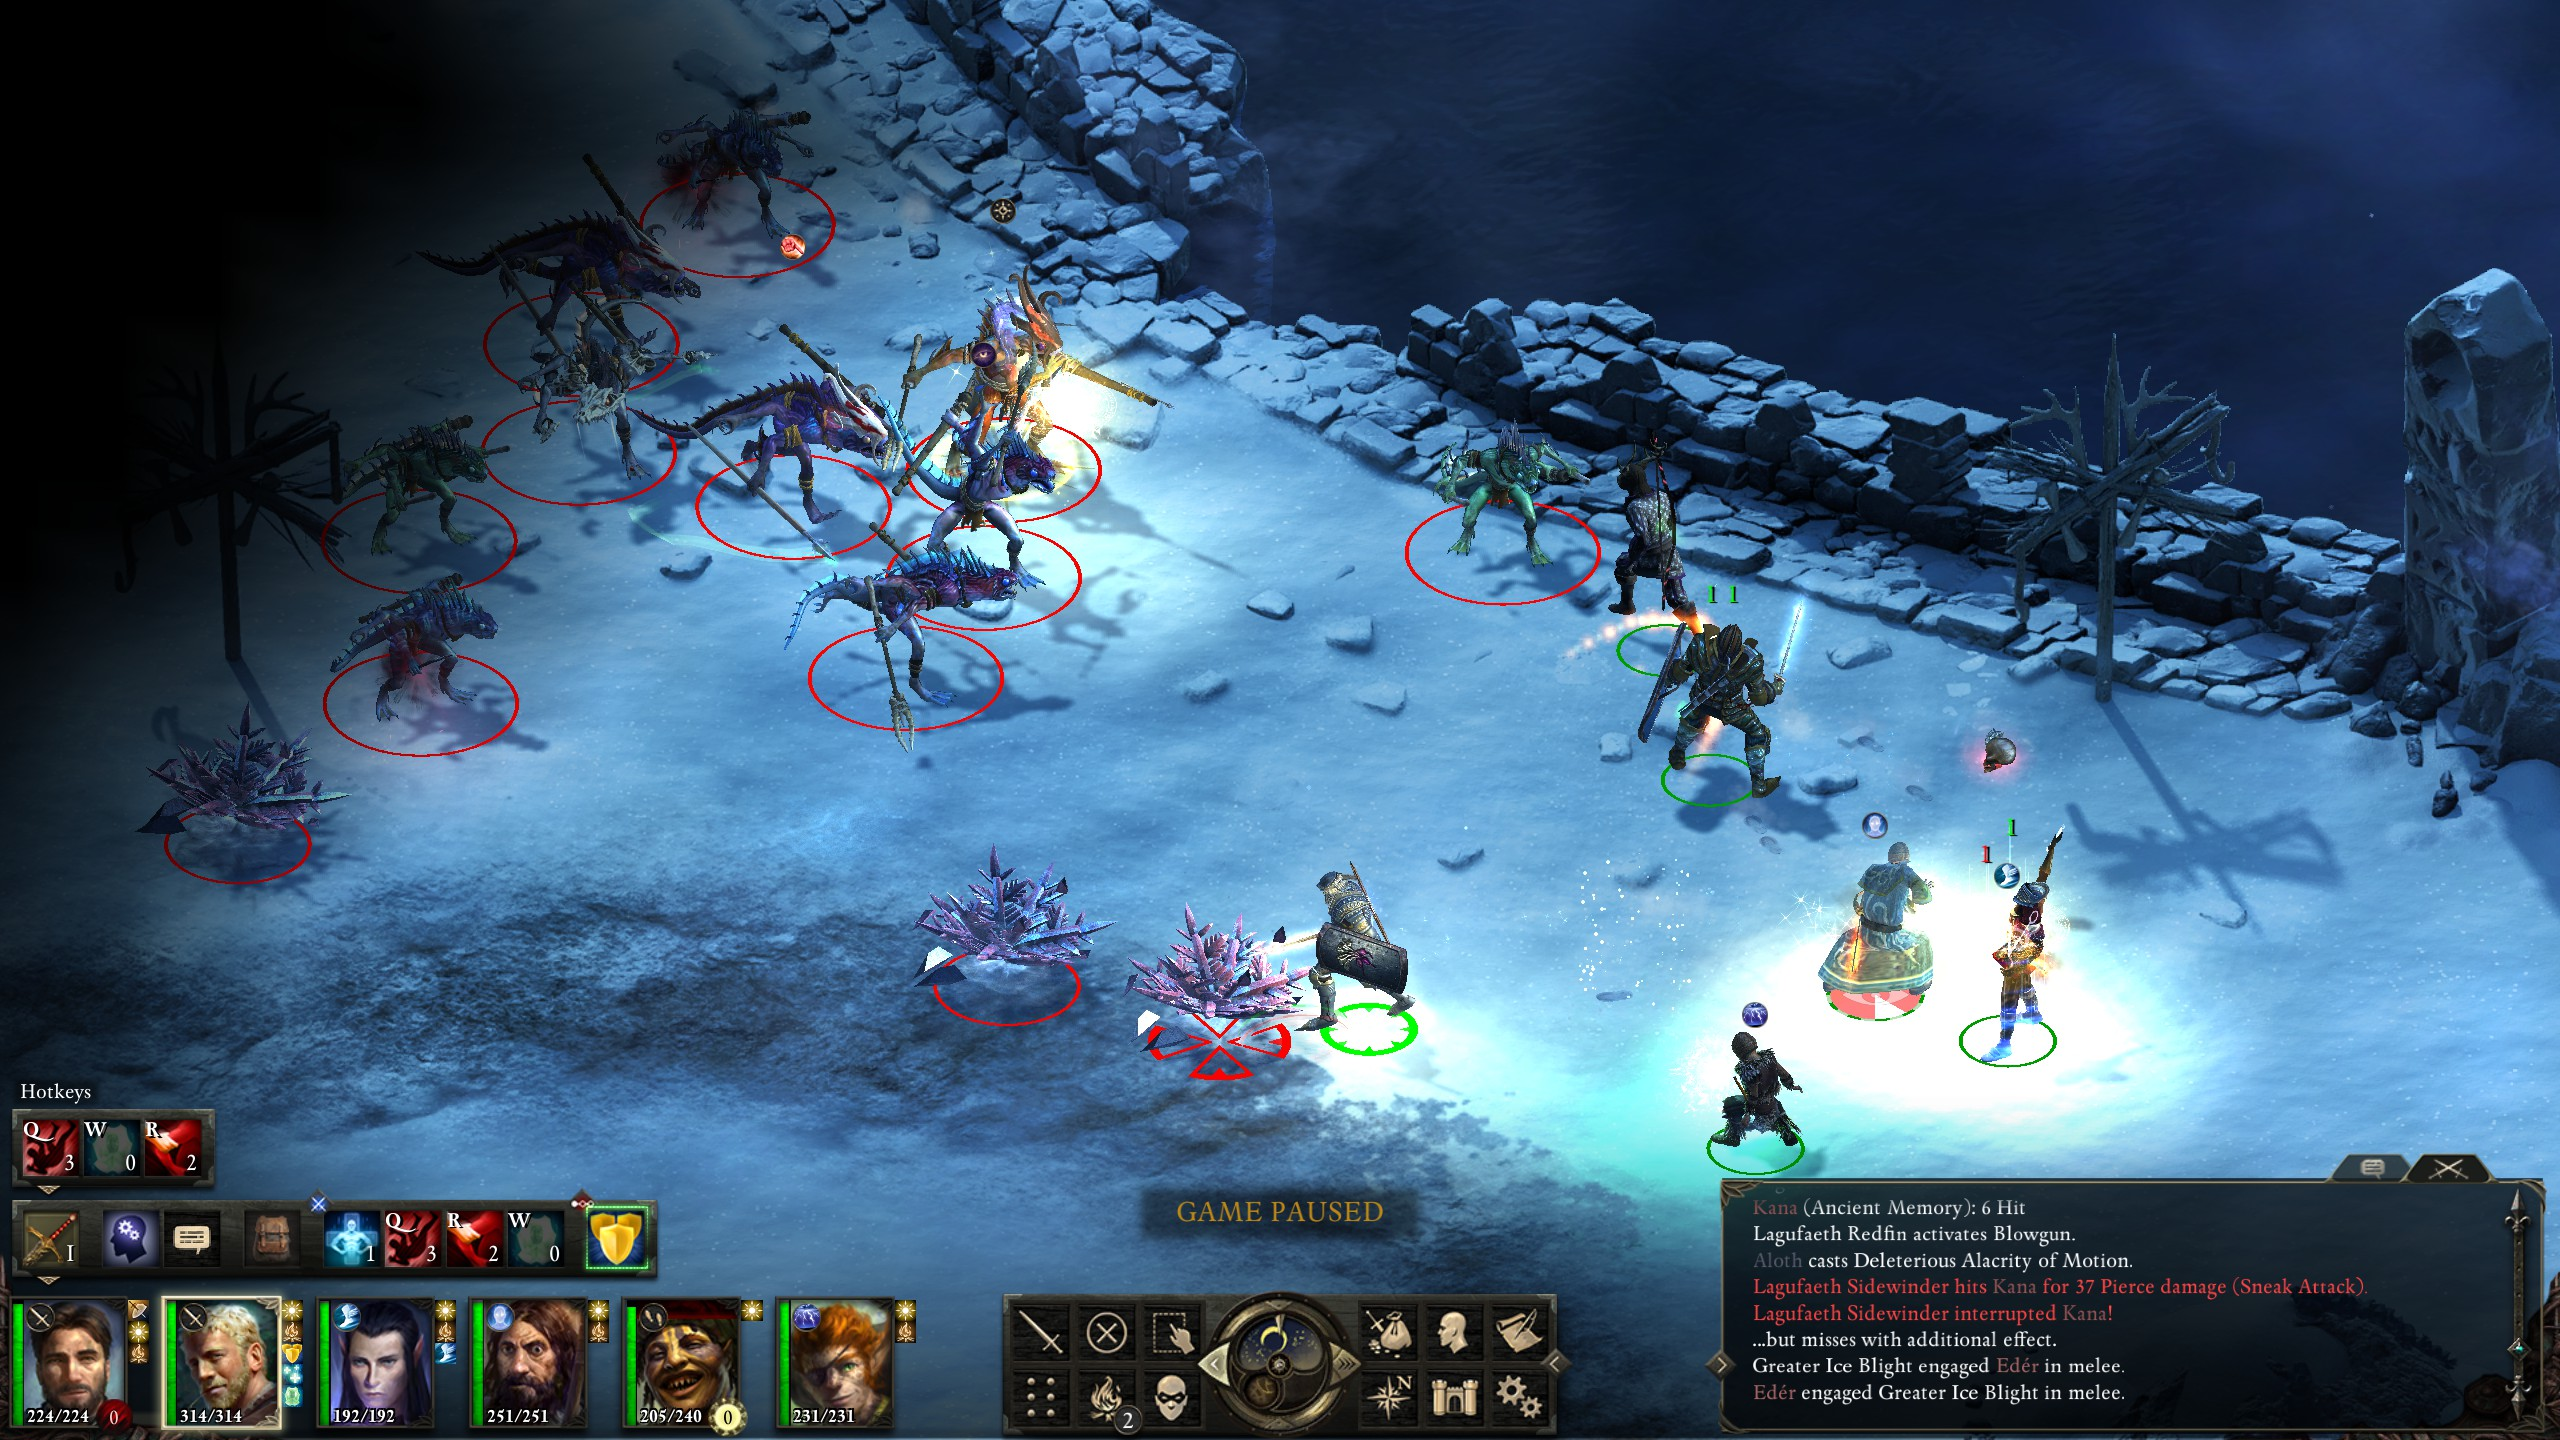
\includegraphics[scale=0.33]{files/blog/2020_01_18_poe_potd_wmpt2/2020_01_18_bounty1_1.jpg}
\end{figure}

My monk had difficulties with the paralysis affliction that the creatures liked to use, but a few casts of Aloth's ``Call to Slumber'' quickly gave me the advantage.

\begin{figure}
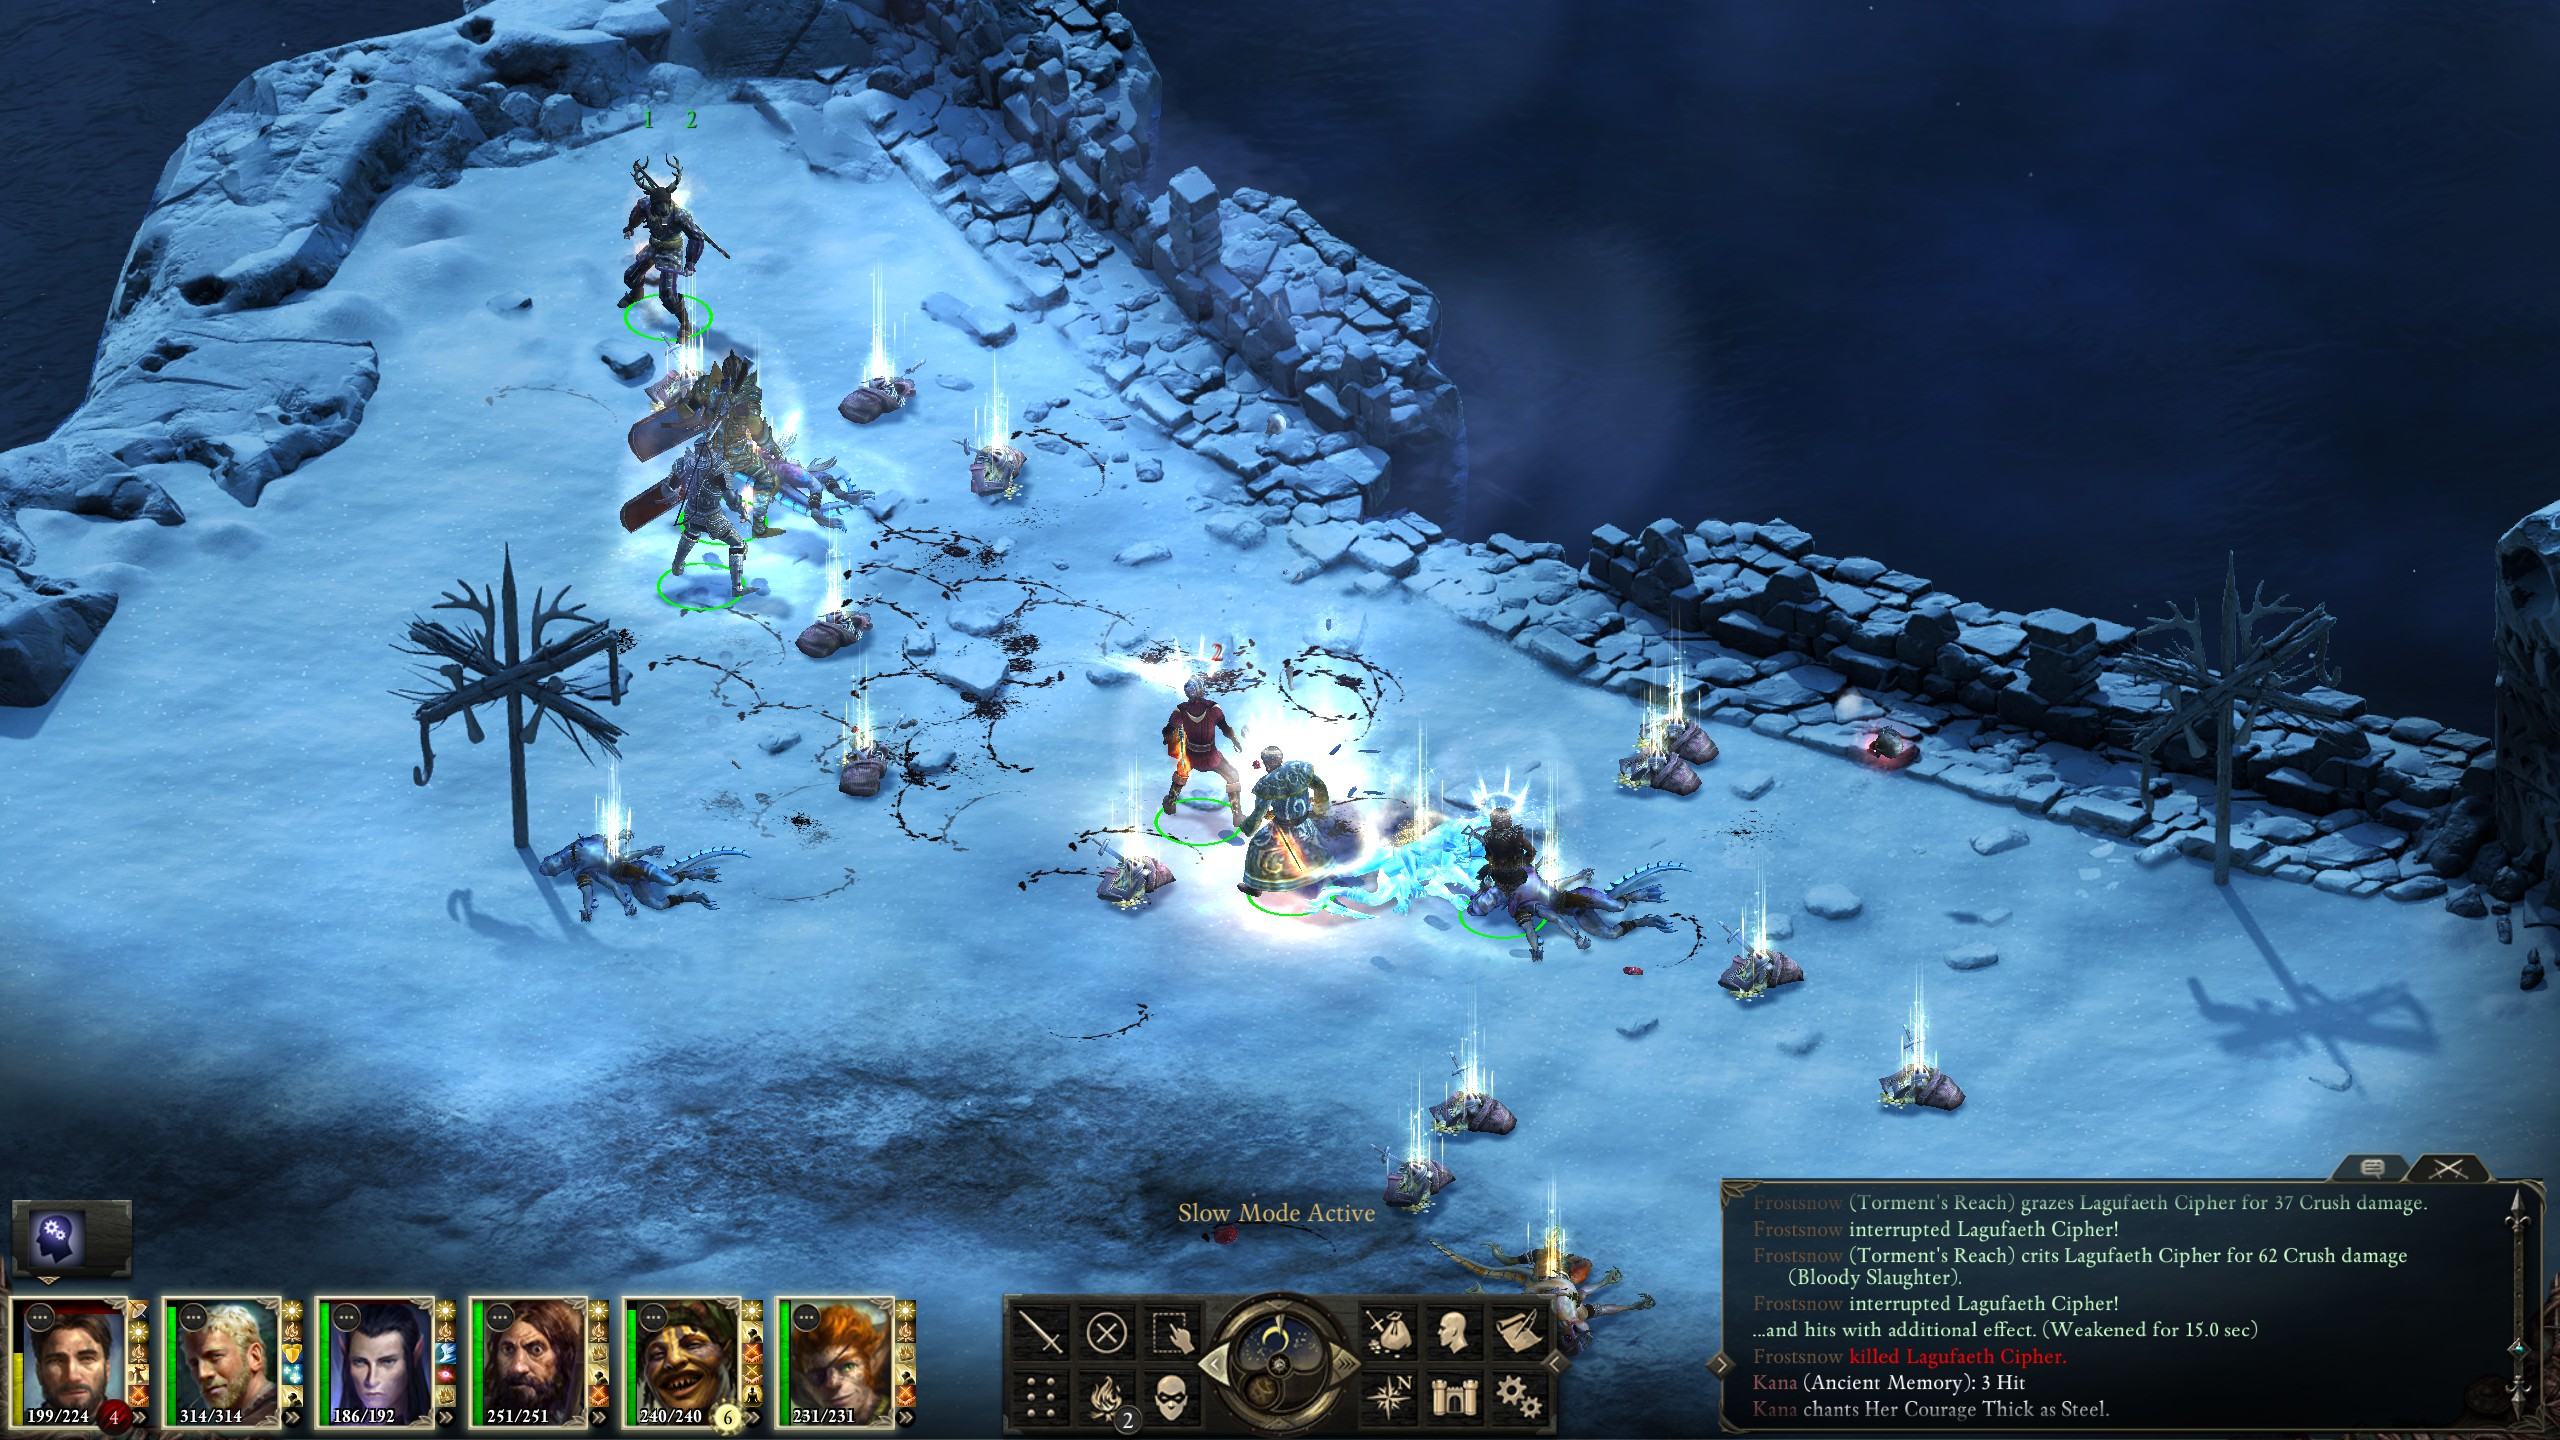
\includegraphics[scale=0.33]{files/blog/2020_01_18_poe_potd_wmpt2/2020_01_18_bounty1_2.jpg}
\end{figure}

After finishing off the lagufaeth, I then headed to the next bounty, a giant ice blight named the Terror of Whitestone Hollow.

\begin{figure}
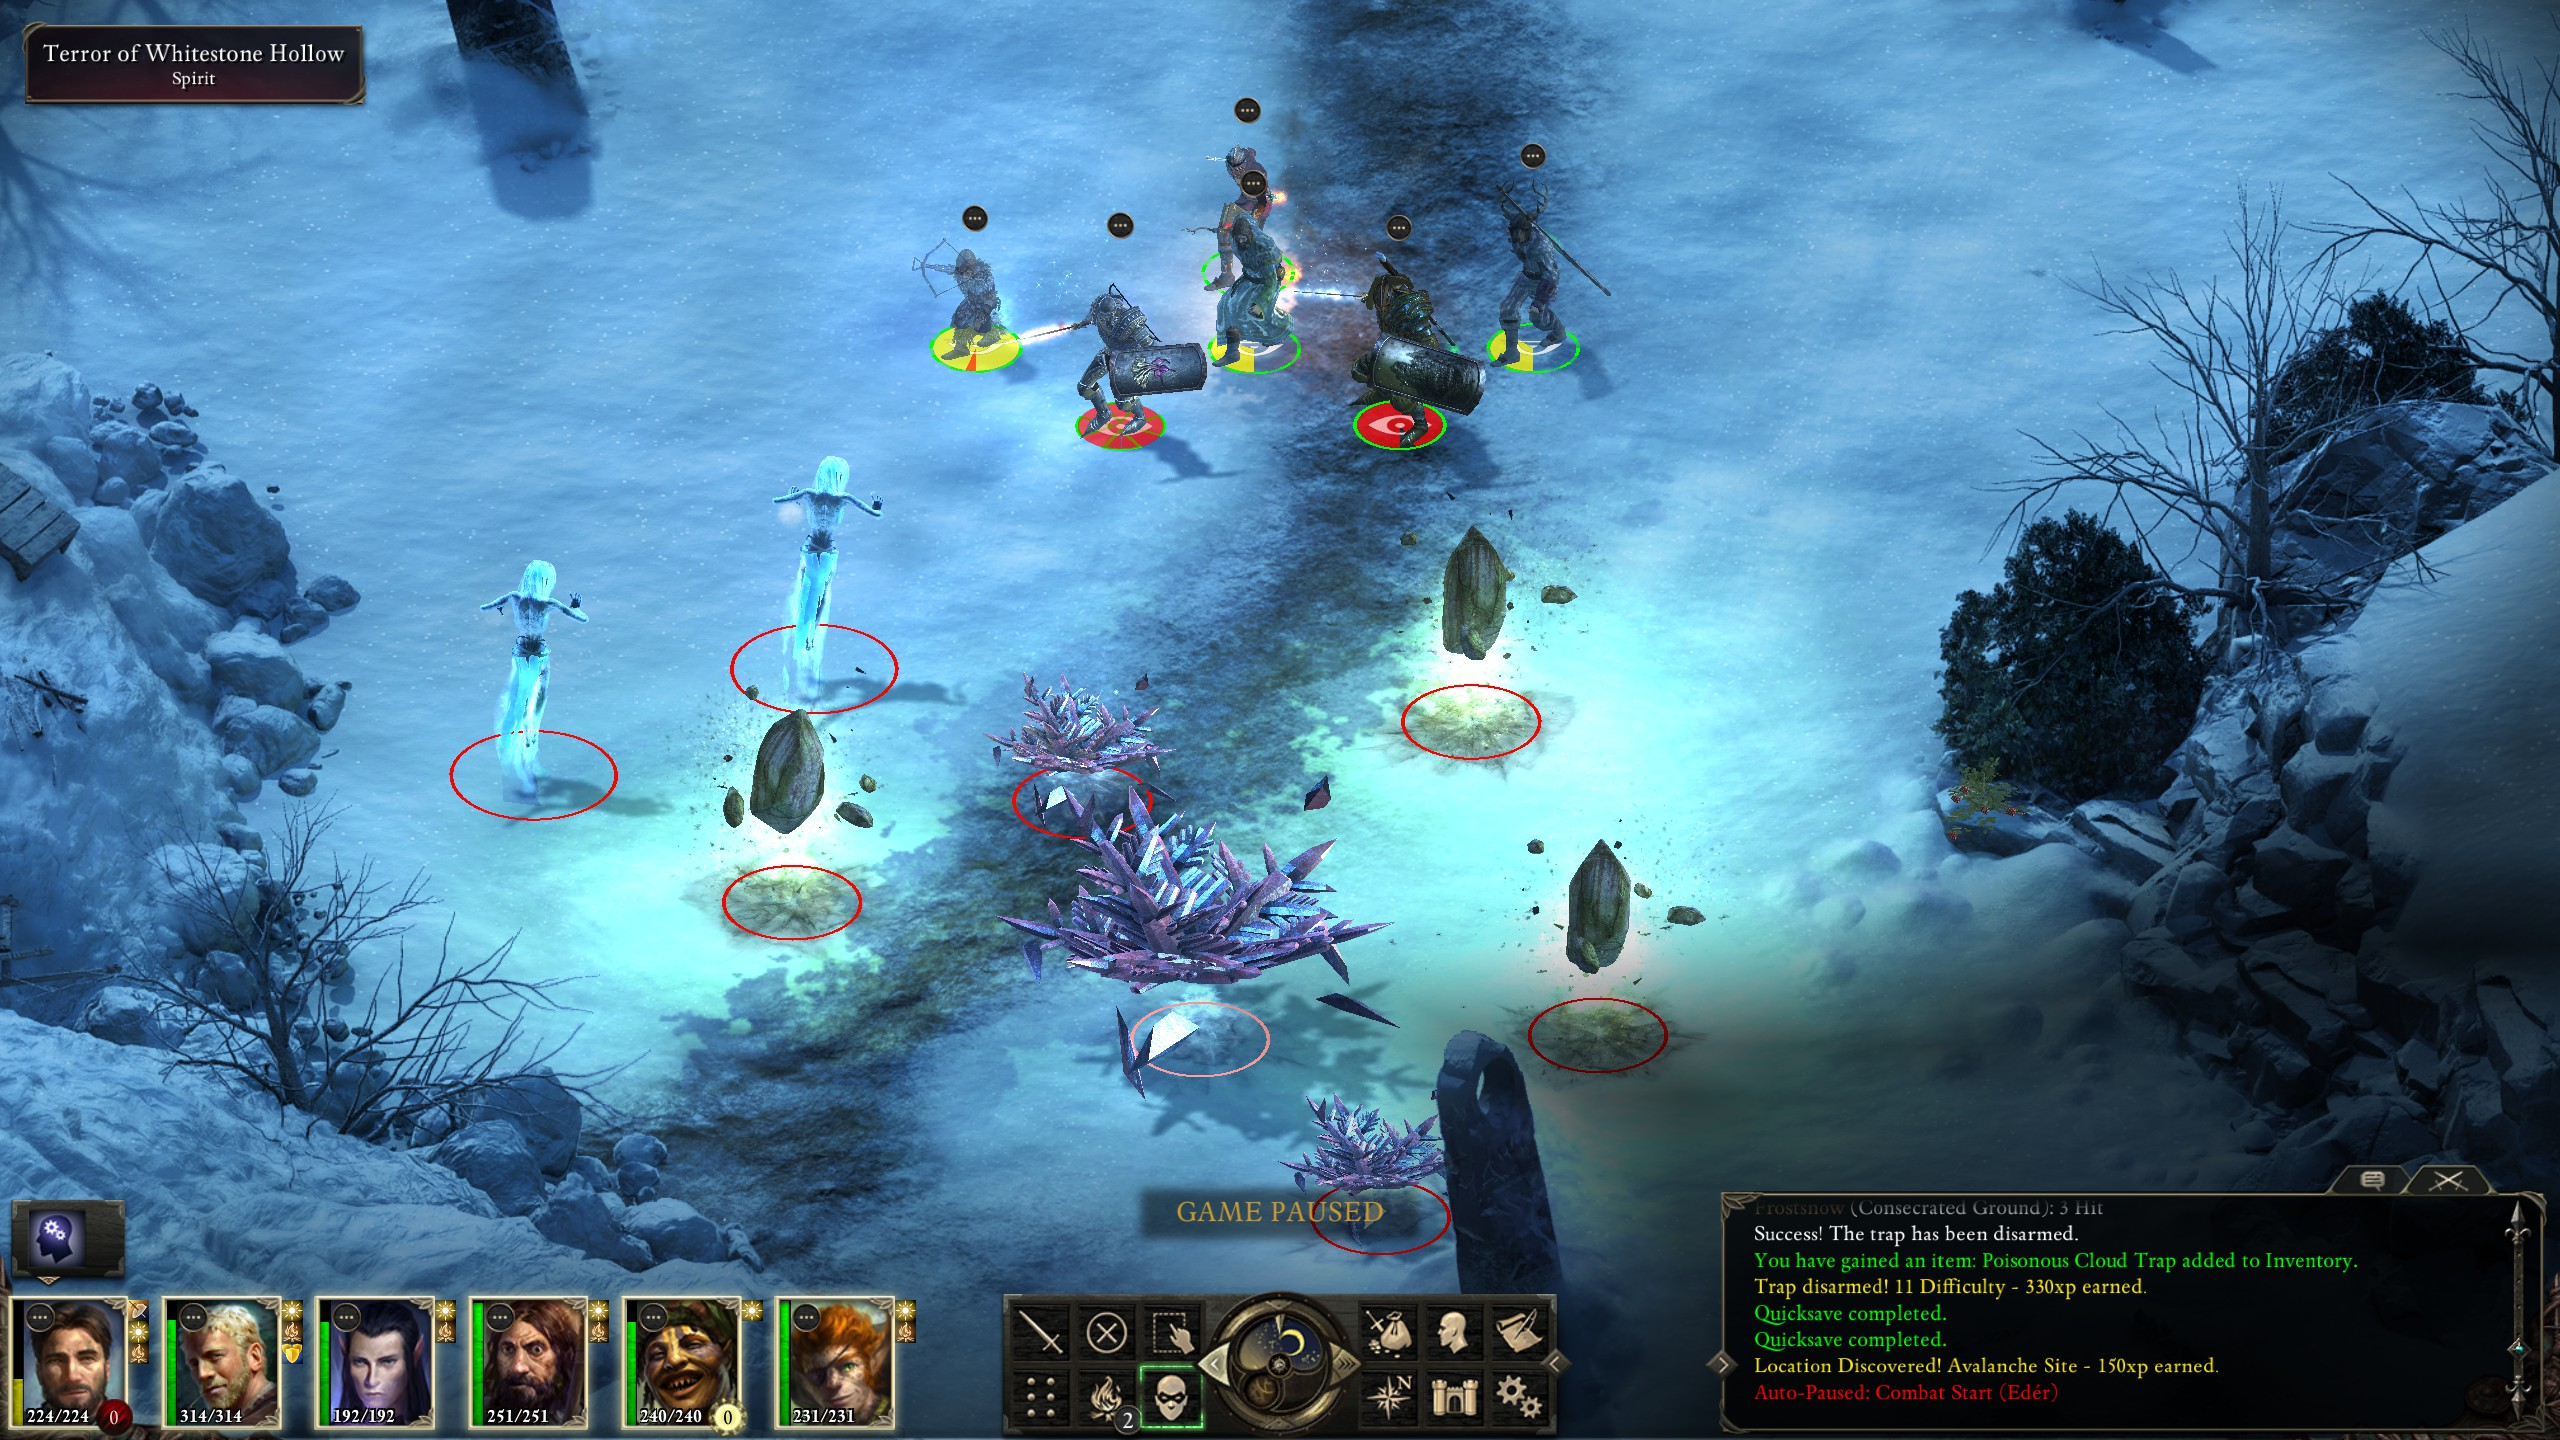
\includegraphics[scale=0.33]{files/blog/2020_01_18_poe_potd_wmpt2/2020_01_18_bounty2_1.jpg}
\end{figure}

The blights were slow and susceptible to unconsciousness, but the cean g\^{w}la were not, so I had Aloth's use ``Substantial Phantom'' then had the duplicate summoned by the spell use ``Arduous Delay of Motion'' in order to immobilize the blights.  For the cean g\^{w}la, I had Durance cast ``Prayer Against Imprisonment'' in order to protect against their screams while my Monk summoned Concelhaut in order to crush them with ``Concelhaut's Crushing Doom''.

\begin{figure}
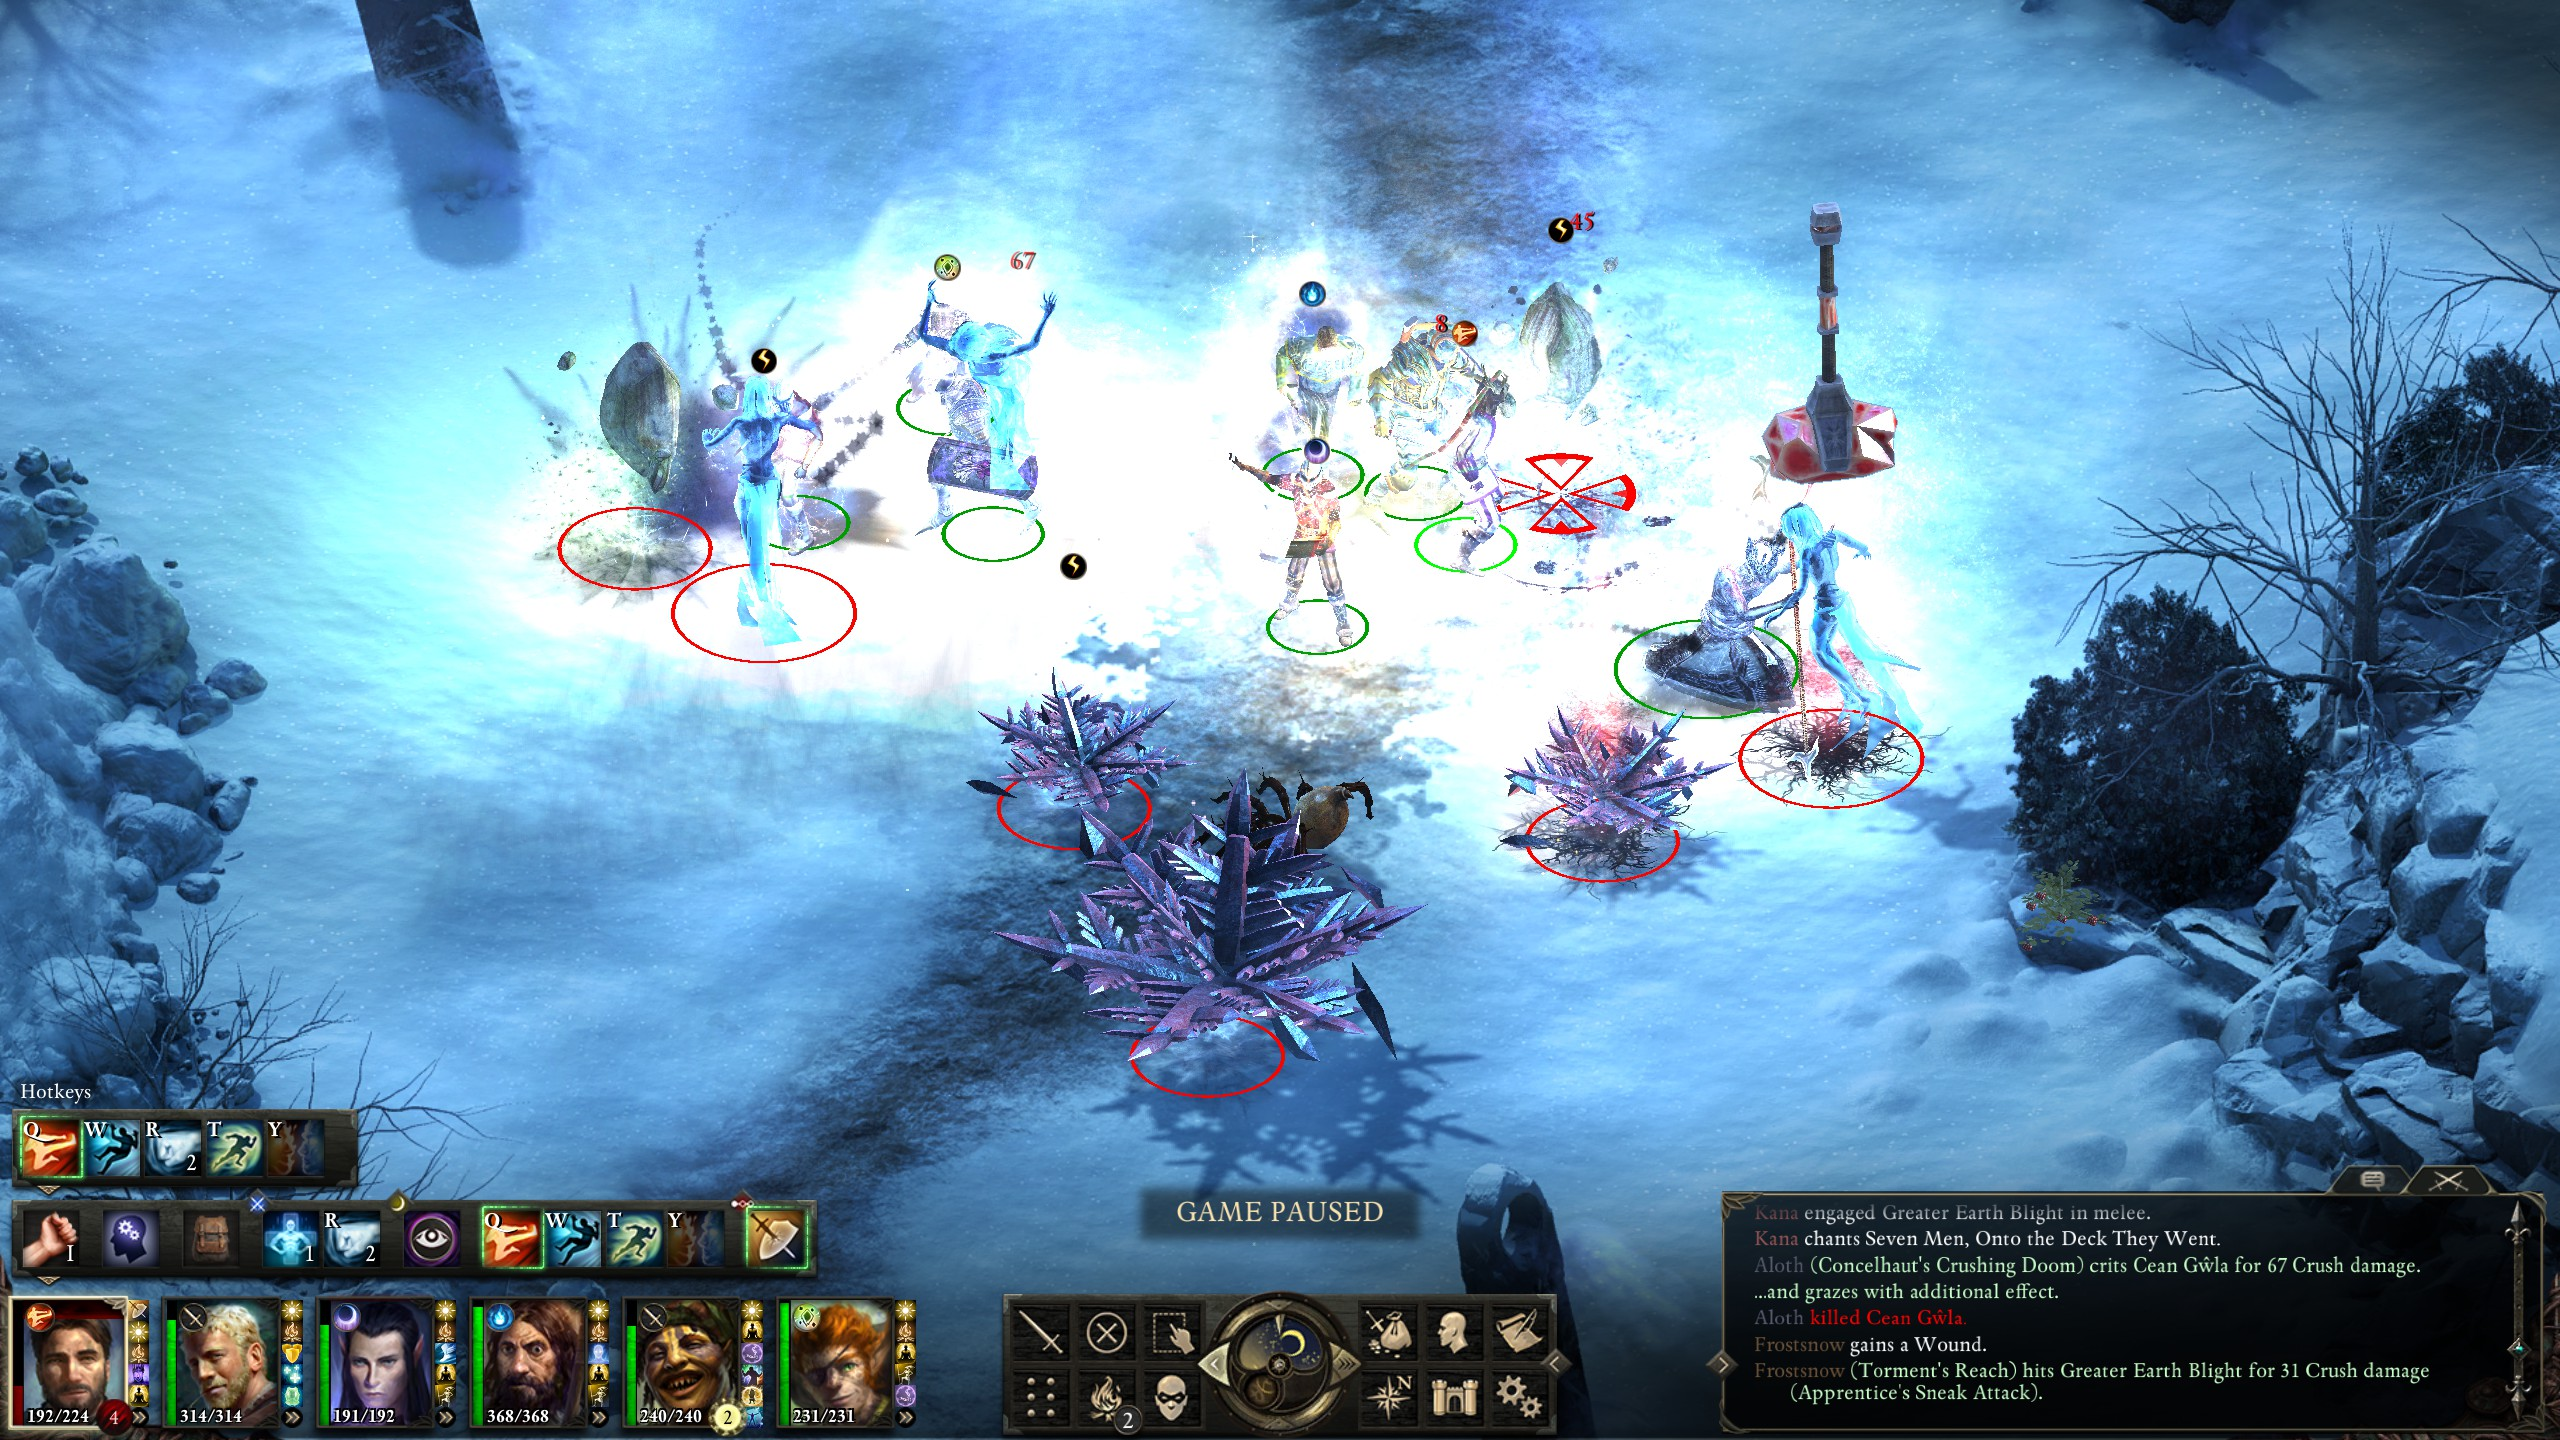
\includegraphics[scale=0.33]{files/blog/2020_01_18_poe_potd_wmpt2/2020_01_18_bounty2_2.jpg}
\end{figure}

This proved to be a highly effective strategy, and I beat the blight and its minions without taking much damage.

\begin{figure}
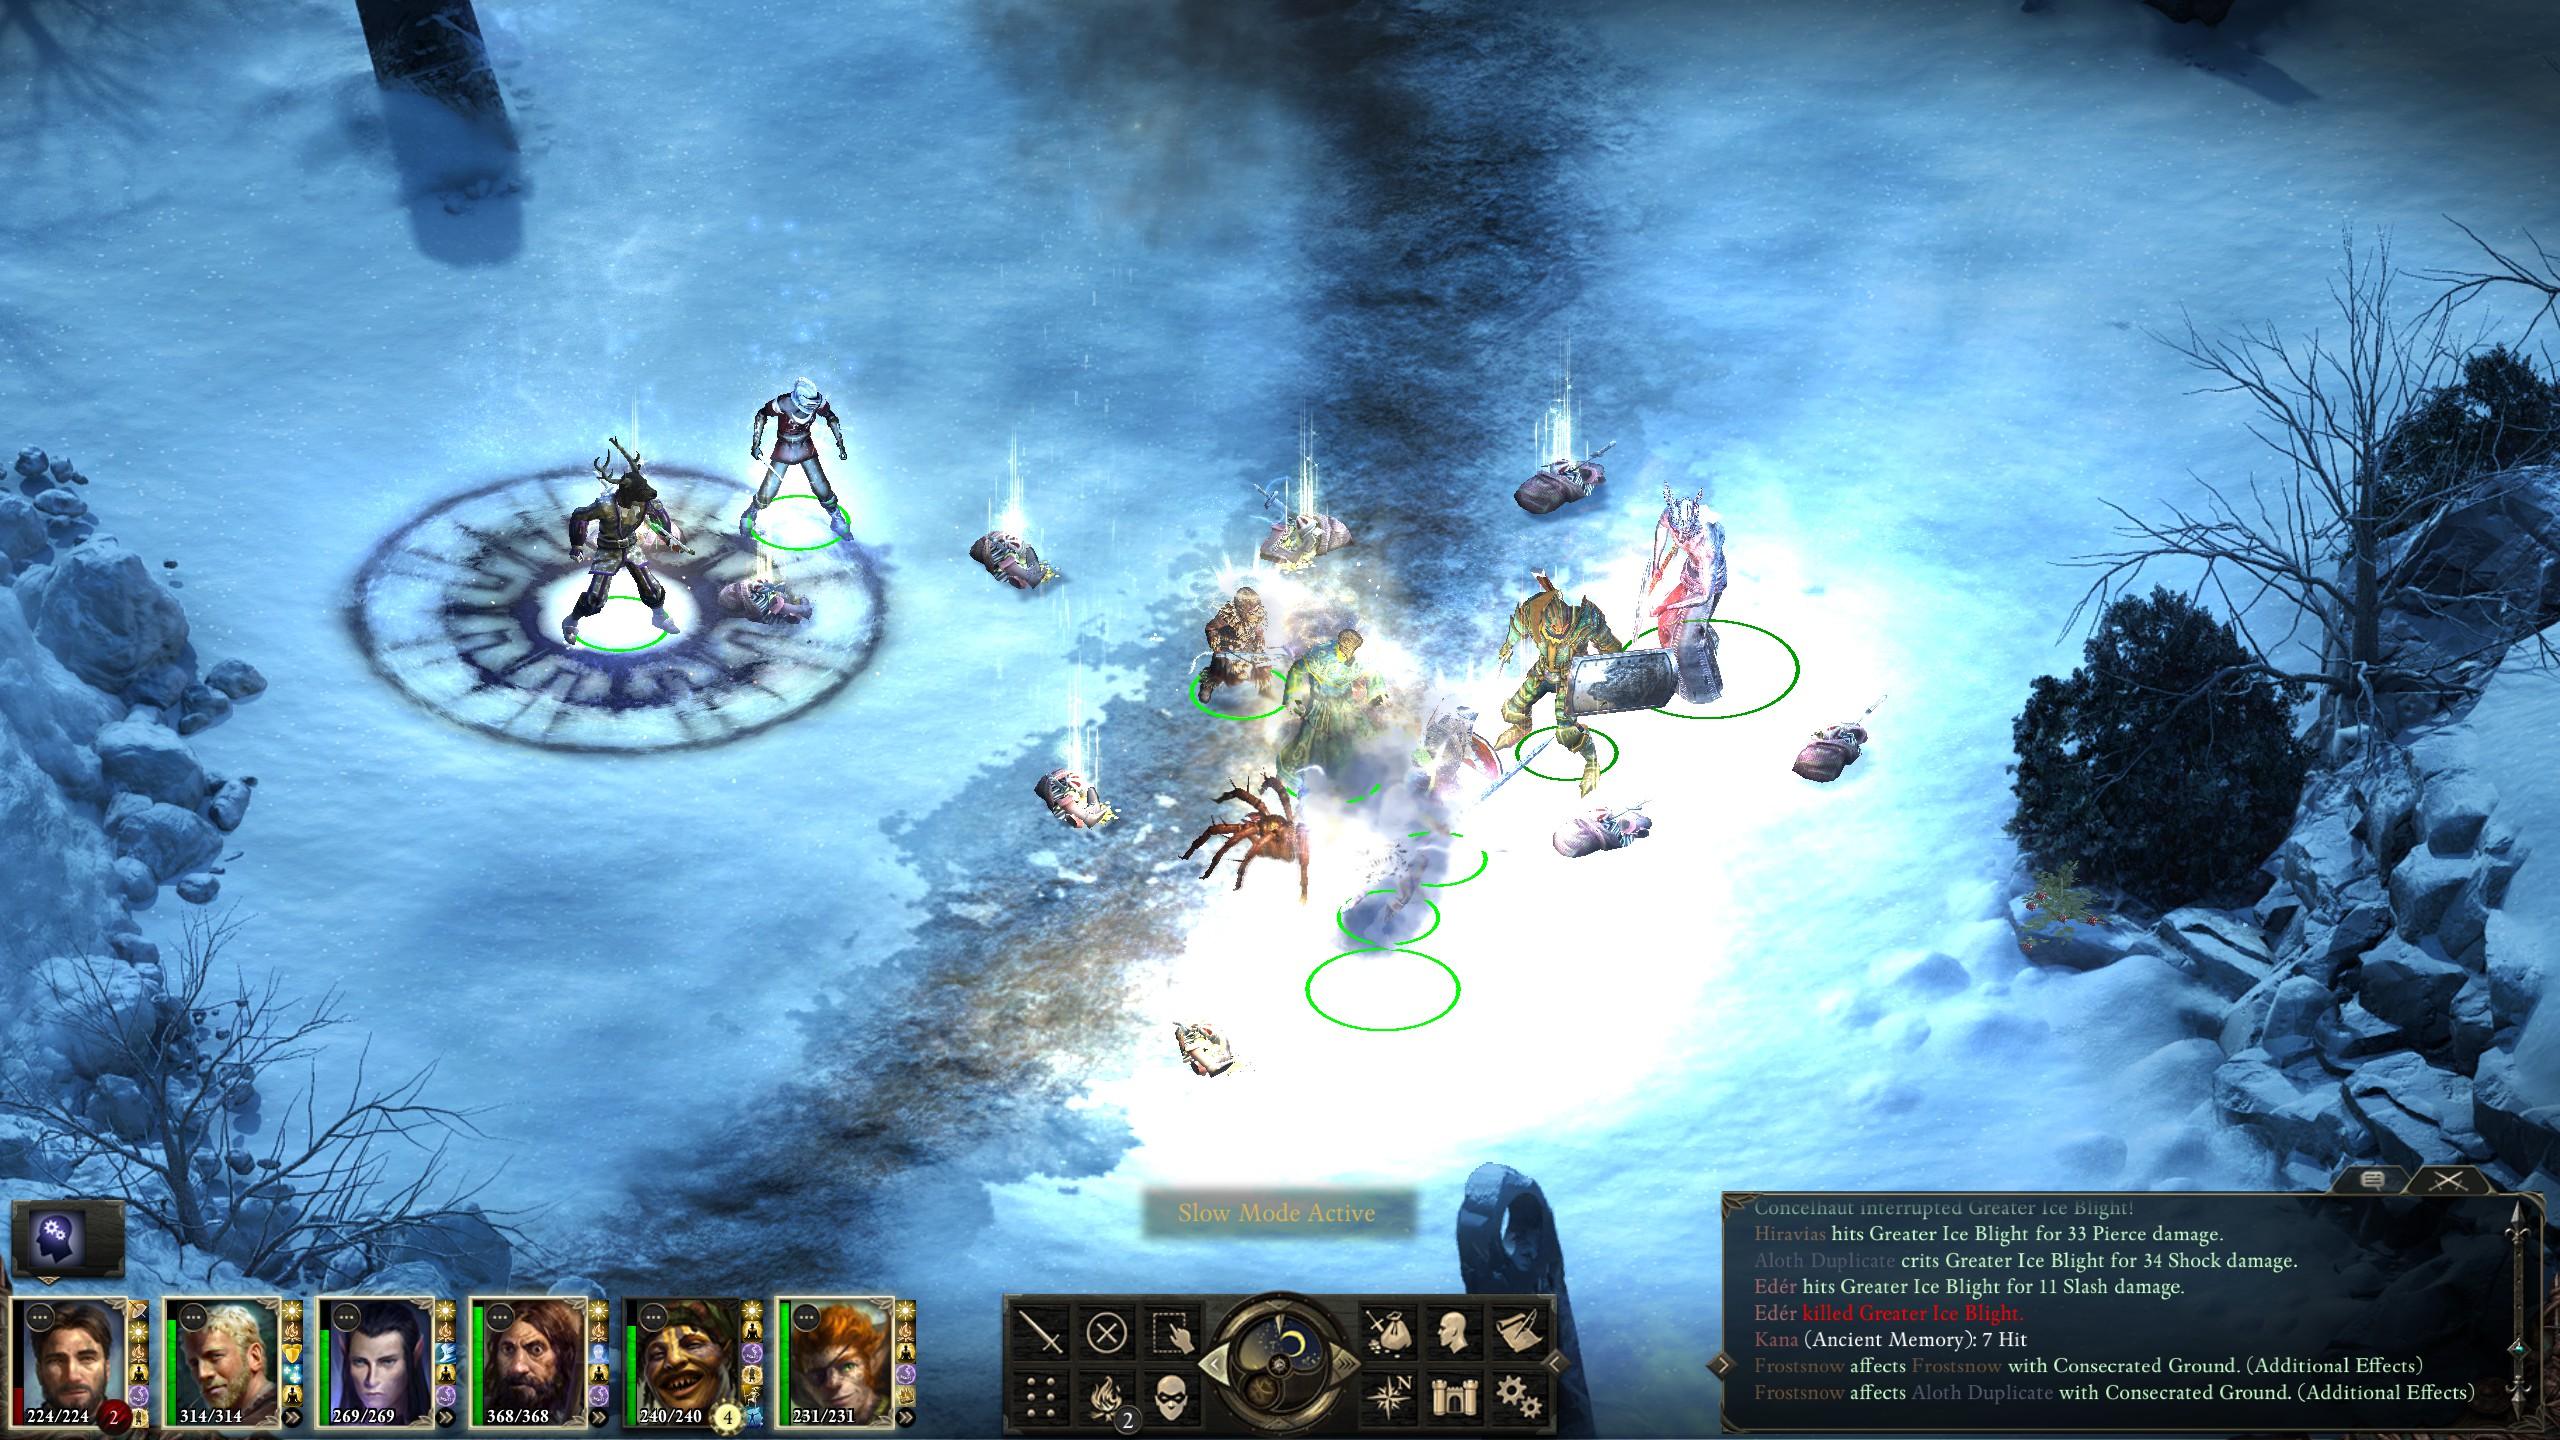
\includegraphics[scale=0.33]{files/blog/2020_01_18_poe_potd_wmpt2/2020_01_18_bounty2_3.jpg}
\end{figure}

Since I'd cleared the bounties in the area, I also cleared out the rest of Whitestone Hollow as well.

\begin{figure}
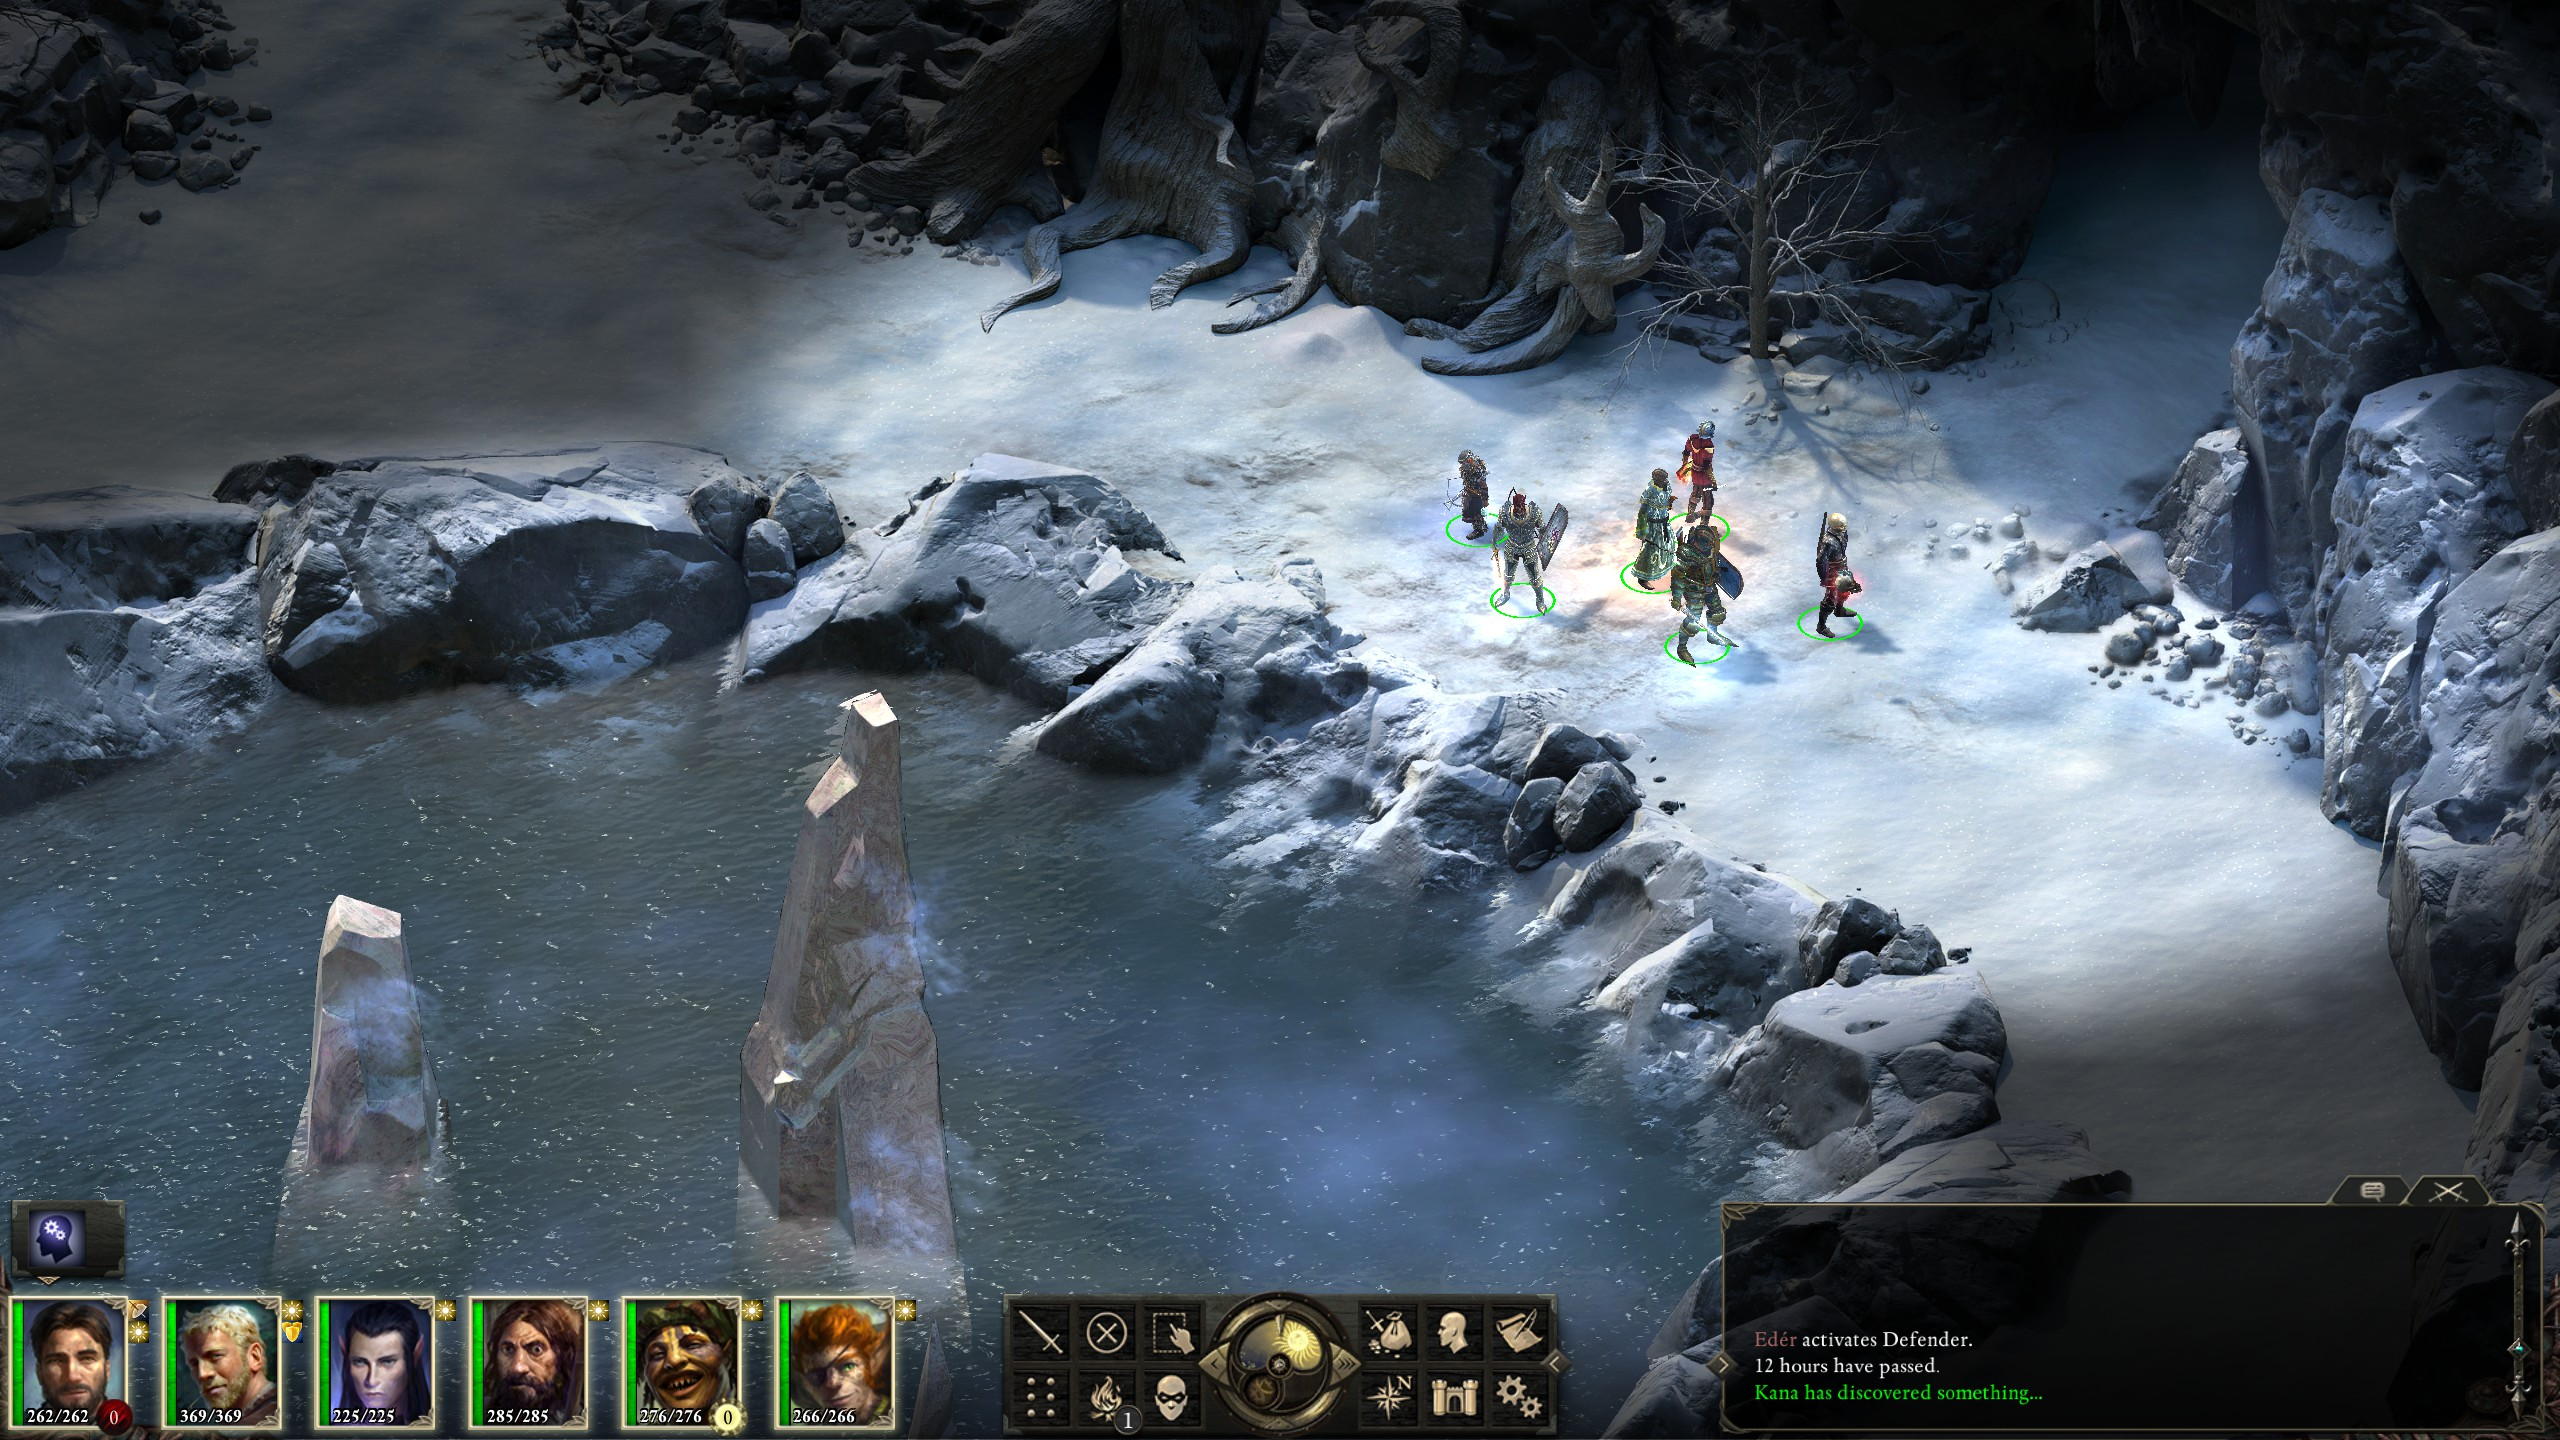
\includegraphics[scale=0.33]{files/blog/2020_01_18_poe_potd_wmpt2/2020_01_18_whitestone.jpg}
\end{figure}

The next and final two bounties were the difficult ones.  First up was Roedwith, leader of Magran's Faithful.

\begin{figure}
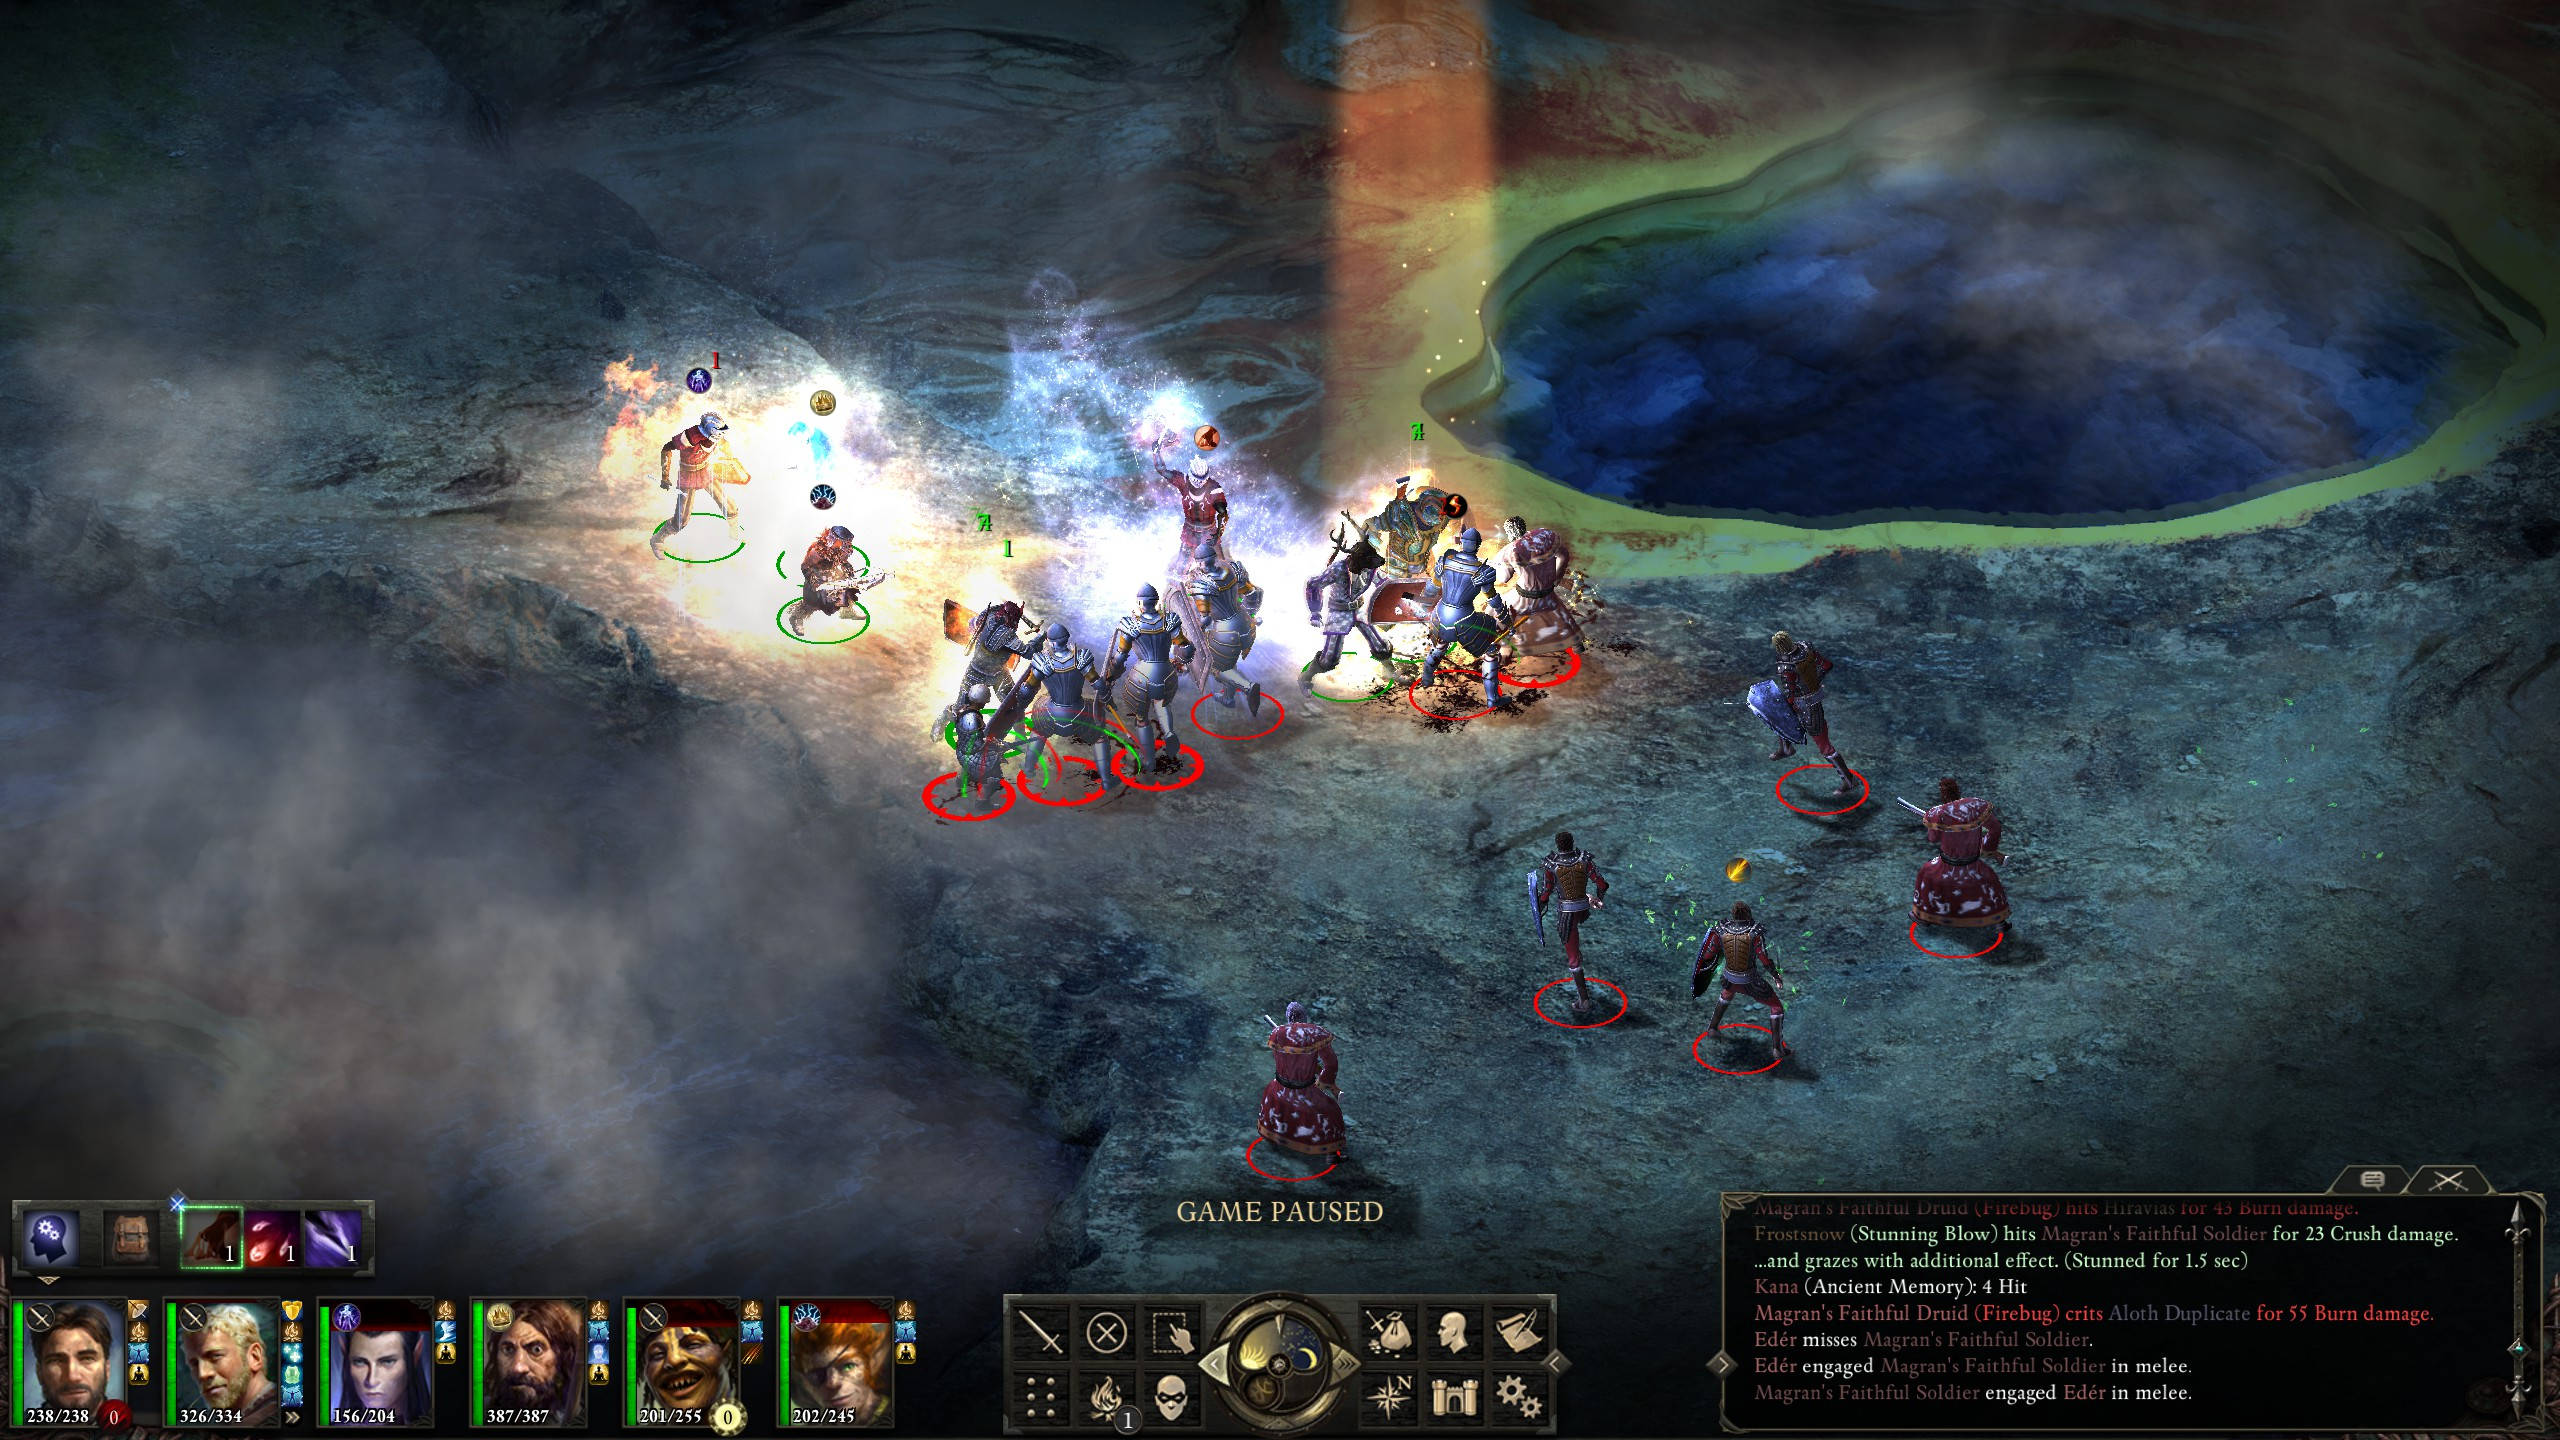
\includegraphics[scale=0.33]{files/blog/2020_01_18_poe_potd_wmpt2/2020_01_18_bounty3_1.jpg}
\end{figure}

Having recently gained 8th-level spells, I decided to make use of Aloth's ``Major Grimoire Imprint'' and stole ``Storm of Holy Fire'' while the battle quickly dissolved into a clustered mess.

\begin{figure}
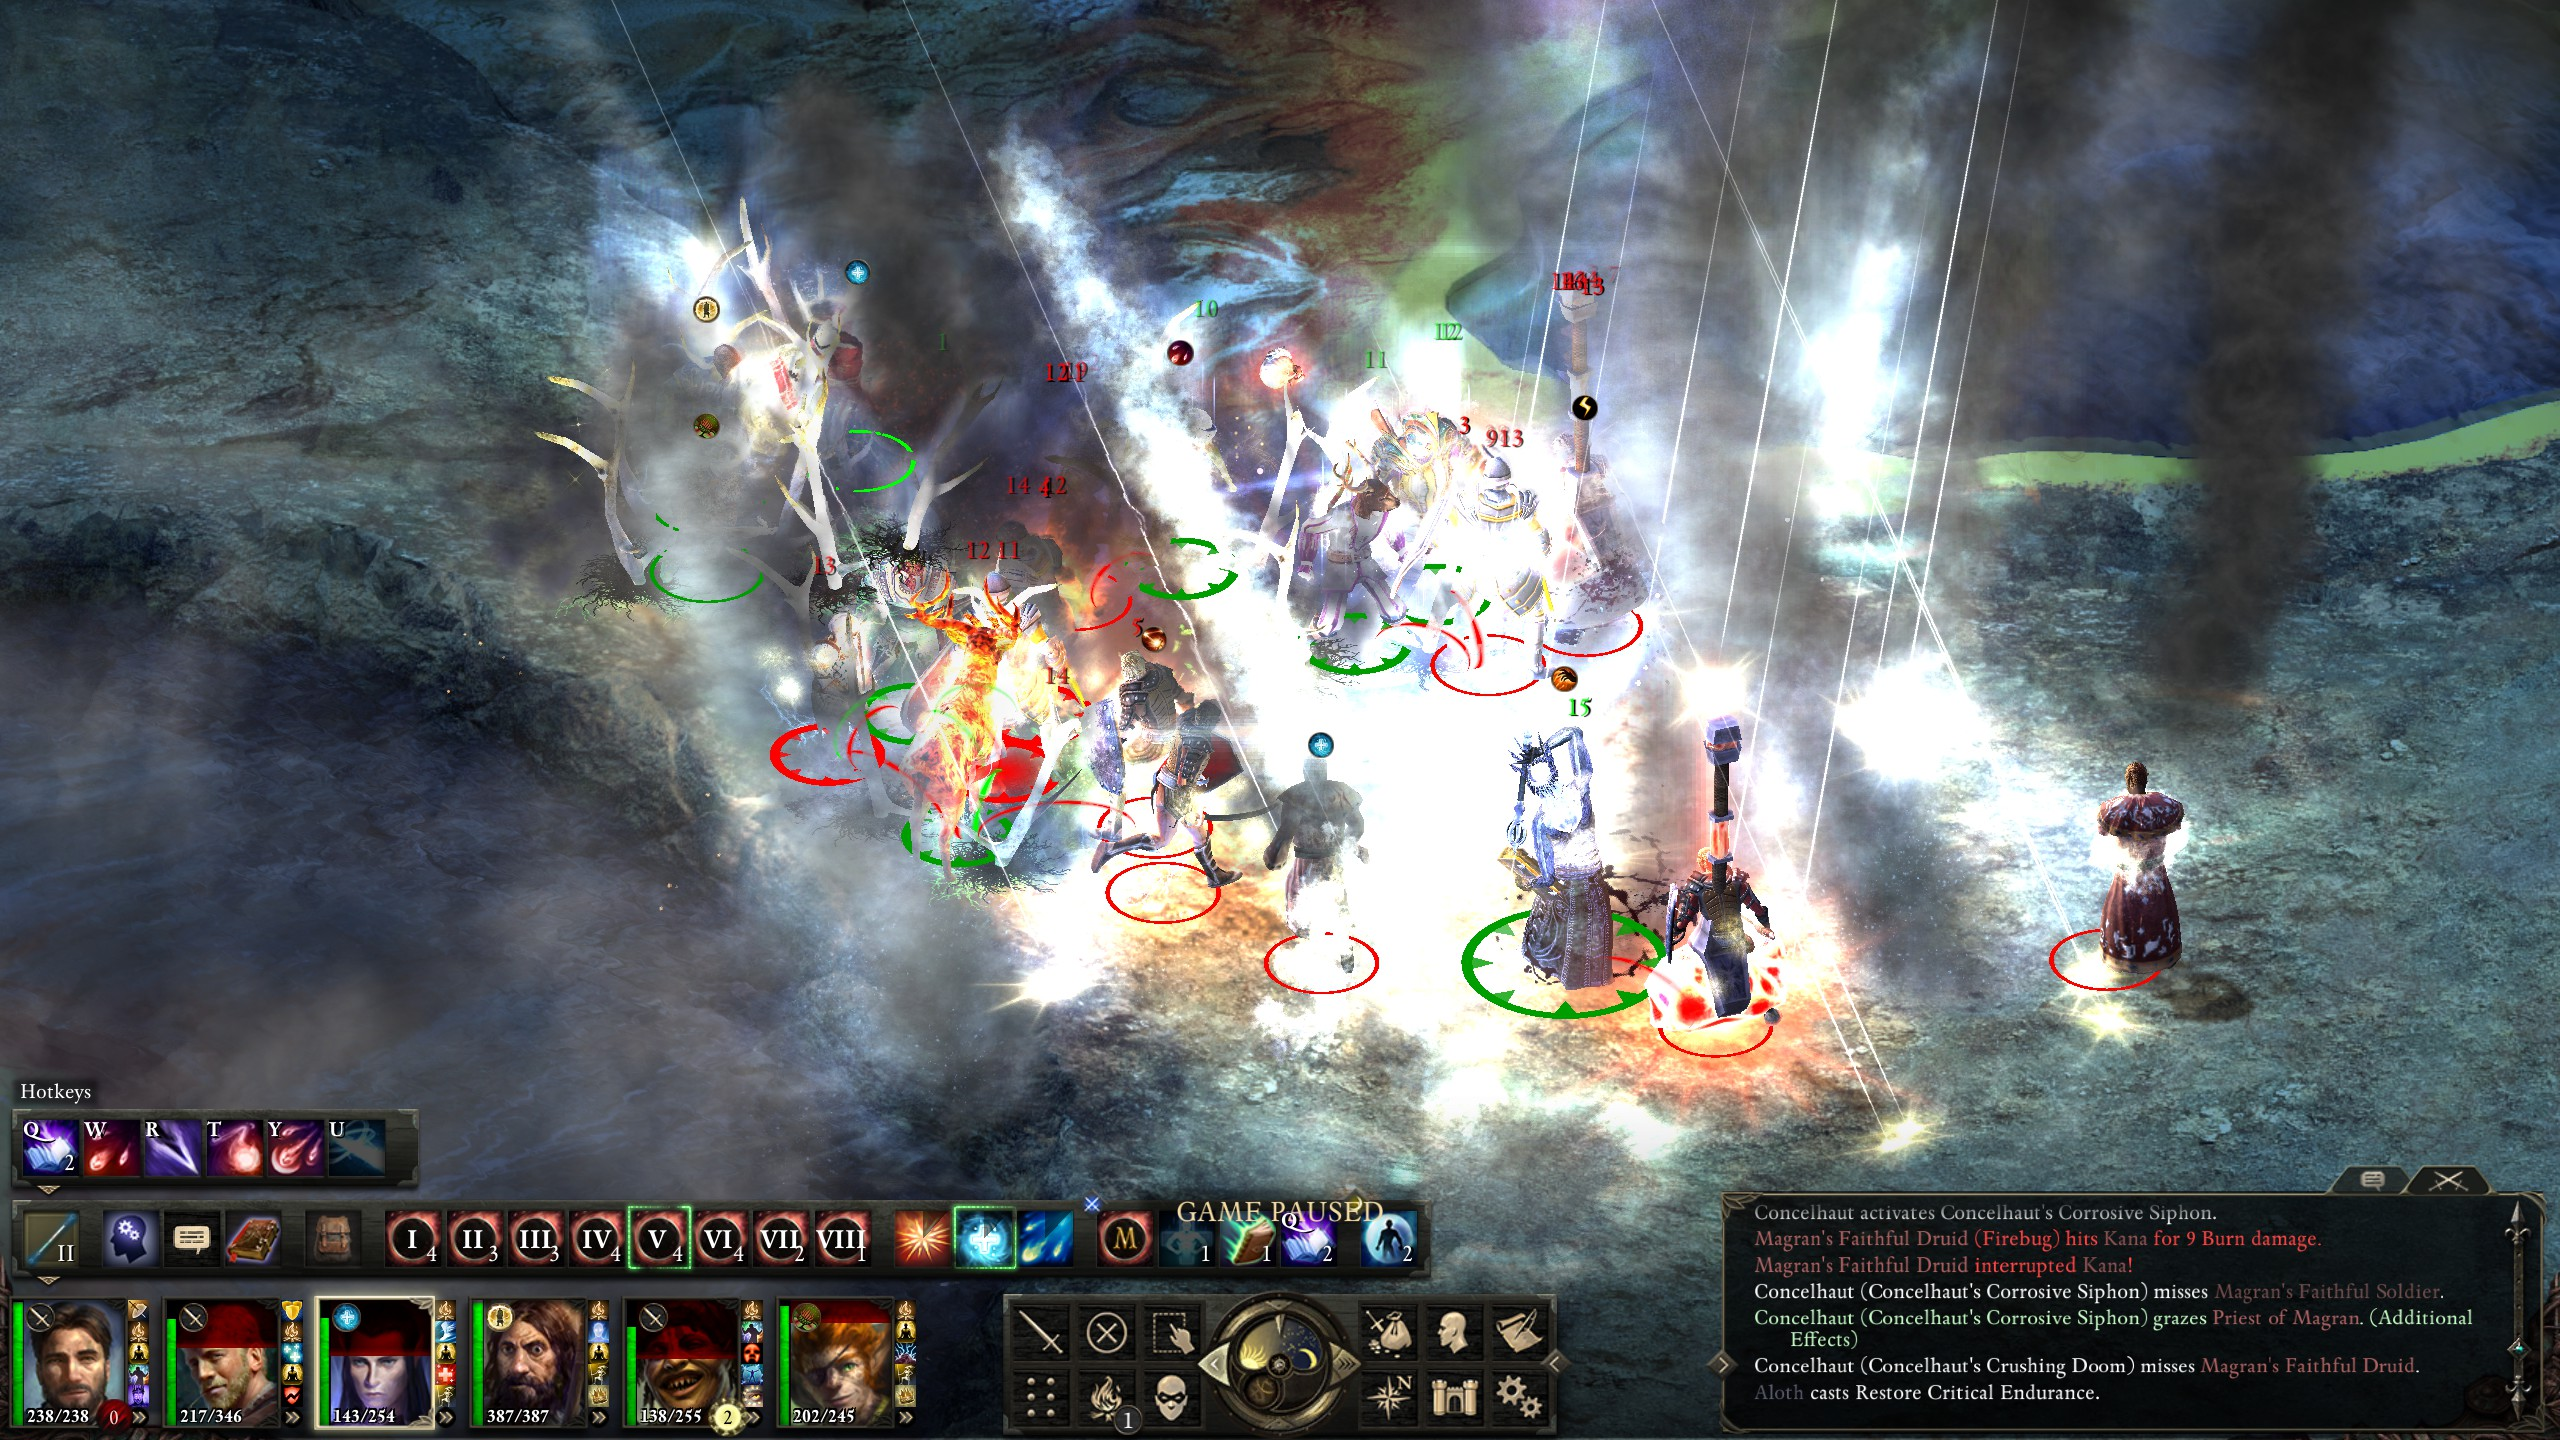
\includegraphics[scale=0.33]{files/blog/2020_01_18_poe_potd_wmpt2/2020_01_18_bounty3_2.jpg}
\end{figure}

Finding the stolen priest's spells unsatisfying, I tried stealing the druid's spells, which ended up giving me unlimited ``Sunlance'' and ``Firebug'' casts for 100 seconds!  I spammed both of them.

\begin{figure}
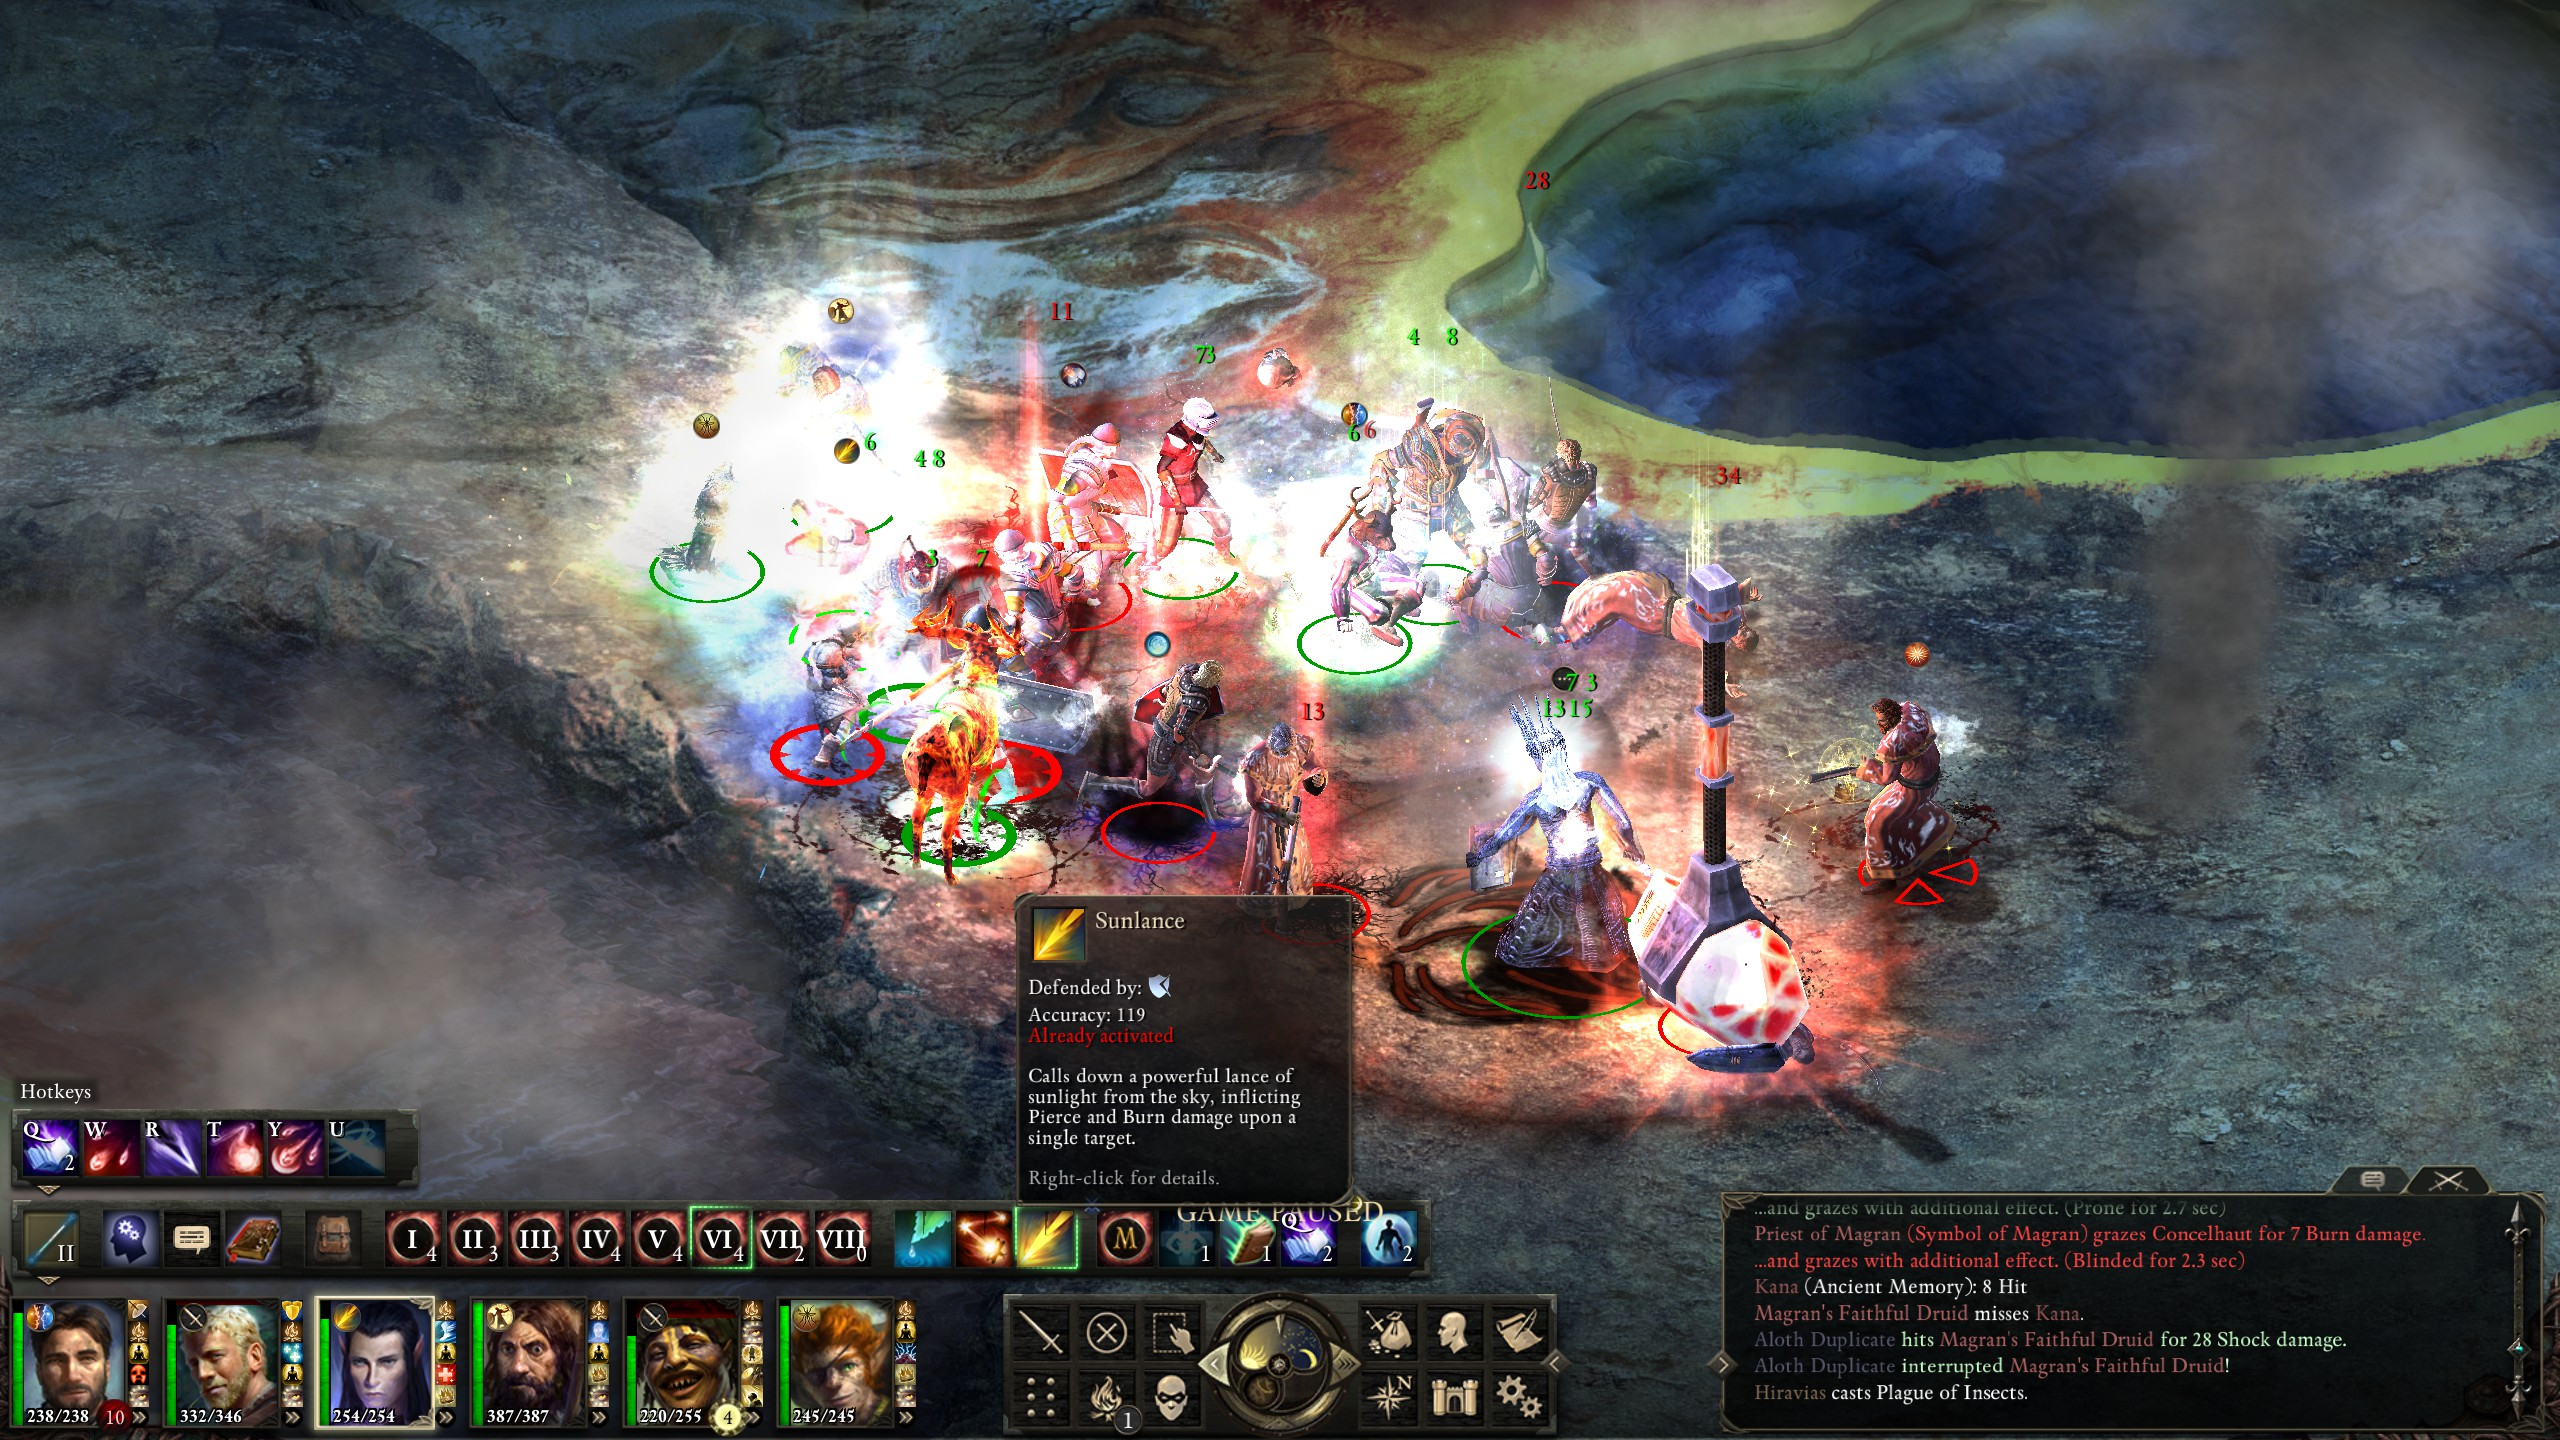
\includegraphics[scale=0.33]{files/blog/2020_01_18_poe_potd_wmpt2/2020_01_18_bounty3_3.jpg}
\end{figure}

Thus with the help of their own druids I managed to beat the cult.

\begin{figure}
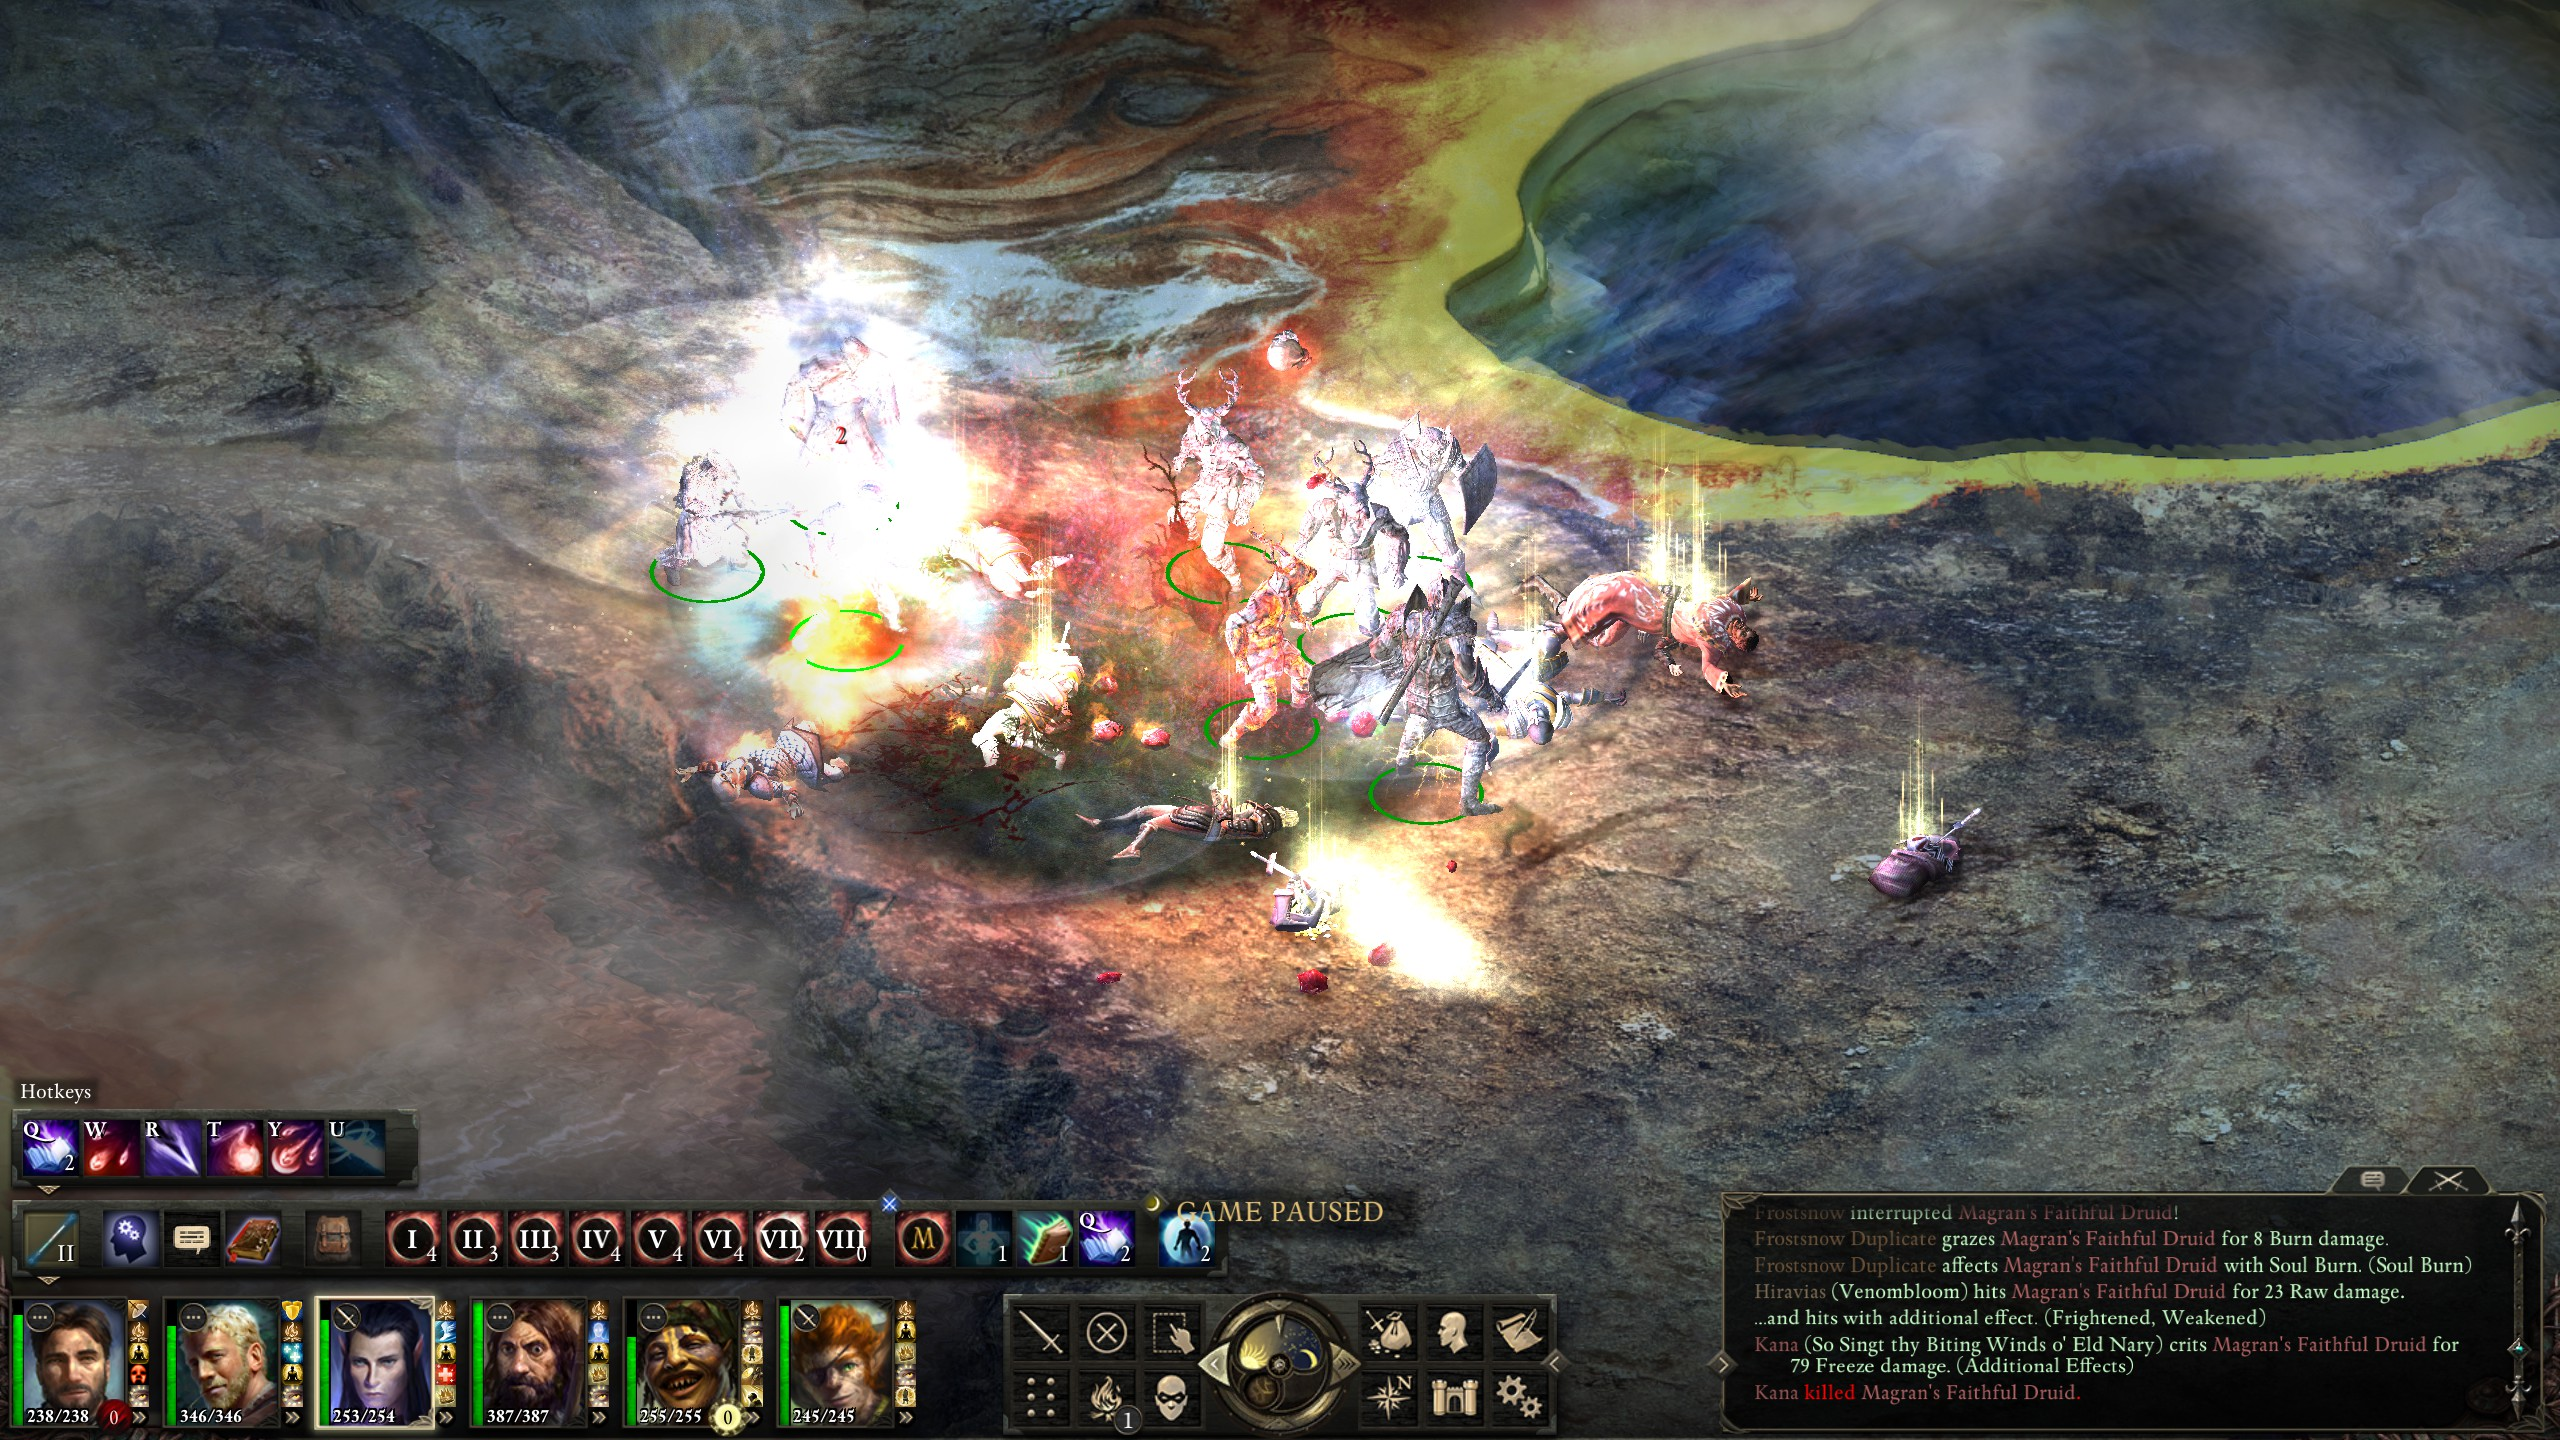
\includegraphics[scale=0.33]{files/blog/2020_01_18_poe_potd_wmpt2/2020_01_18_bounty3_4.jpg}
\end{figure}

The final and most difficult bounty was Brynlod and his deadfire pirates; perhaps Obsidian already knew which area their first expansion would cover?  I recalled this fight being unusually difficult from previous runs, but could not recount the reason.

\begin{figure}
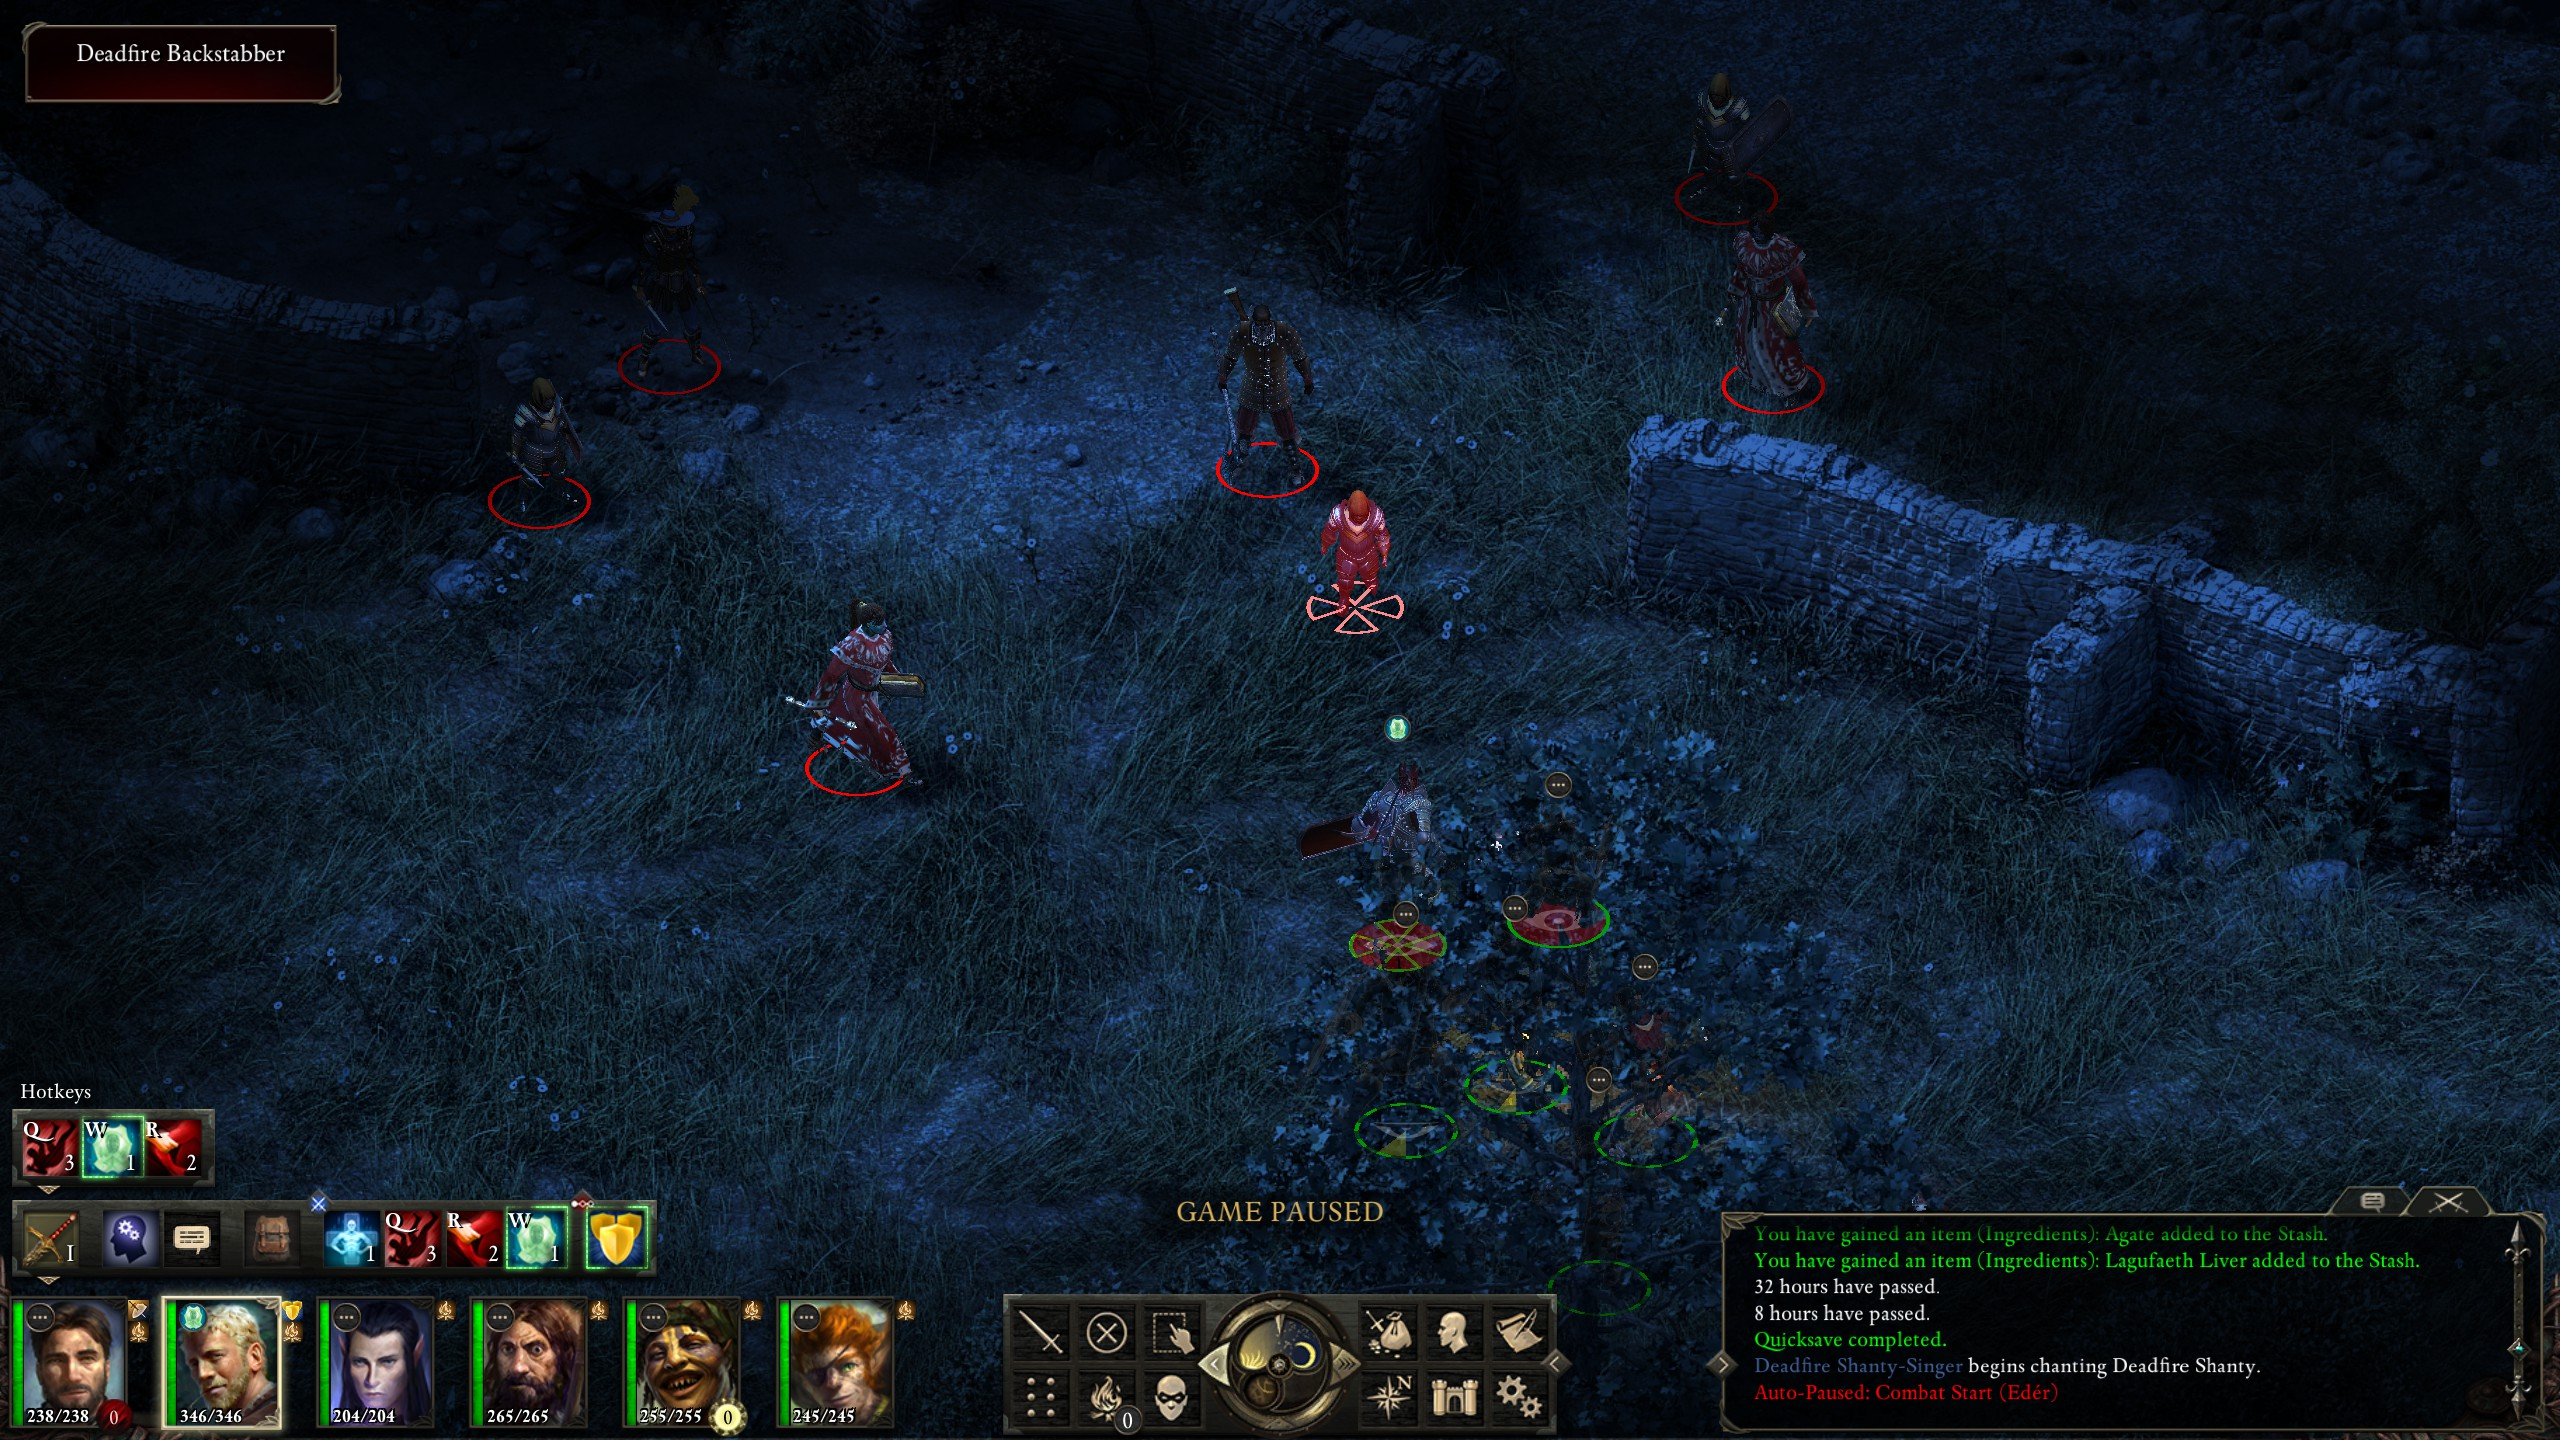
\includegraphics[scale=0.33]{files/blog/2020_01_18_poe_potd_wmpt2/2020_01_18_bounty4_1.jpg}
\end{figure}

About halfway into the fight I realized what exactly was happening.  The three deadfire illusionists were acting as a sort of battle mage; they'd use ``Deleterious Alacrity of Motion'' to quickly cast spells, then ``Essential Phantom'' for some extra damage, then ``Arcane Reflection'' so they couldn't be easily picked off by spells, and finally ``Caedebald's Blackbow'' and ``Citzal's Martial Power'' in order to rapidly deal out massive auto-attack damage.  Oh, and they \emph{all} targeted my monk.

\begin{figure}
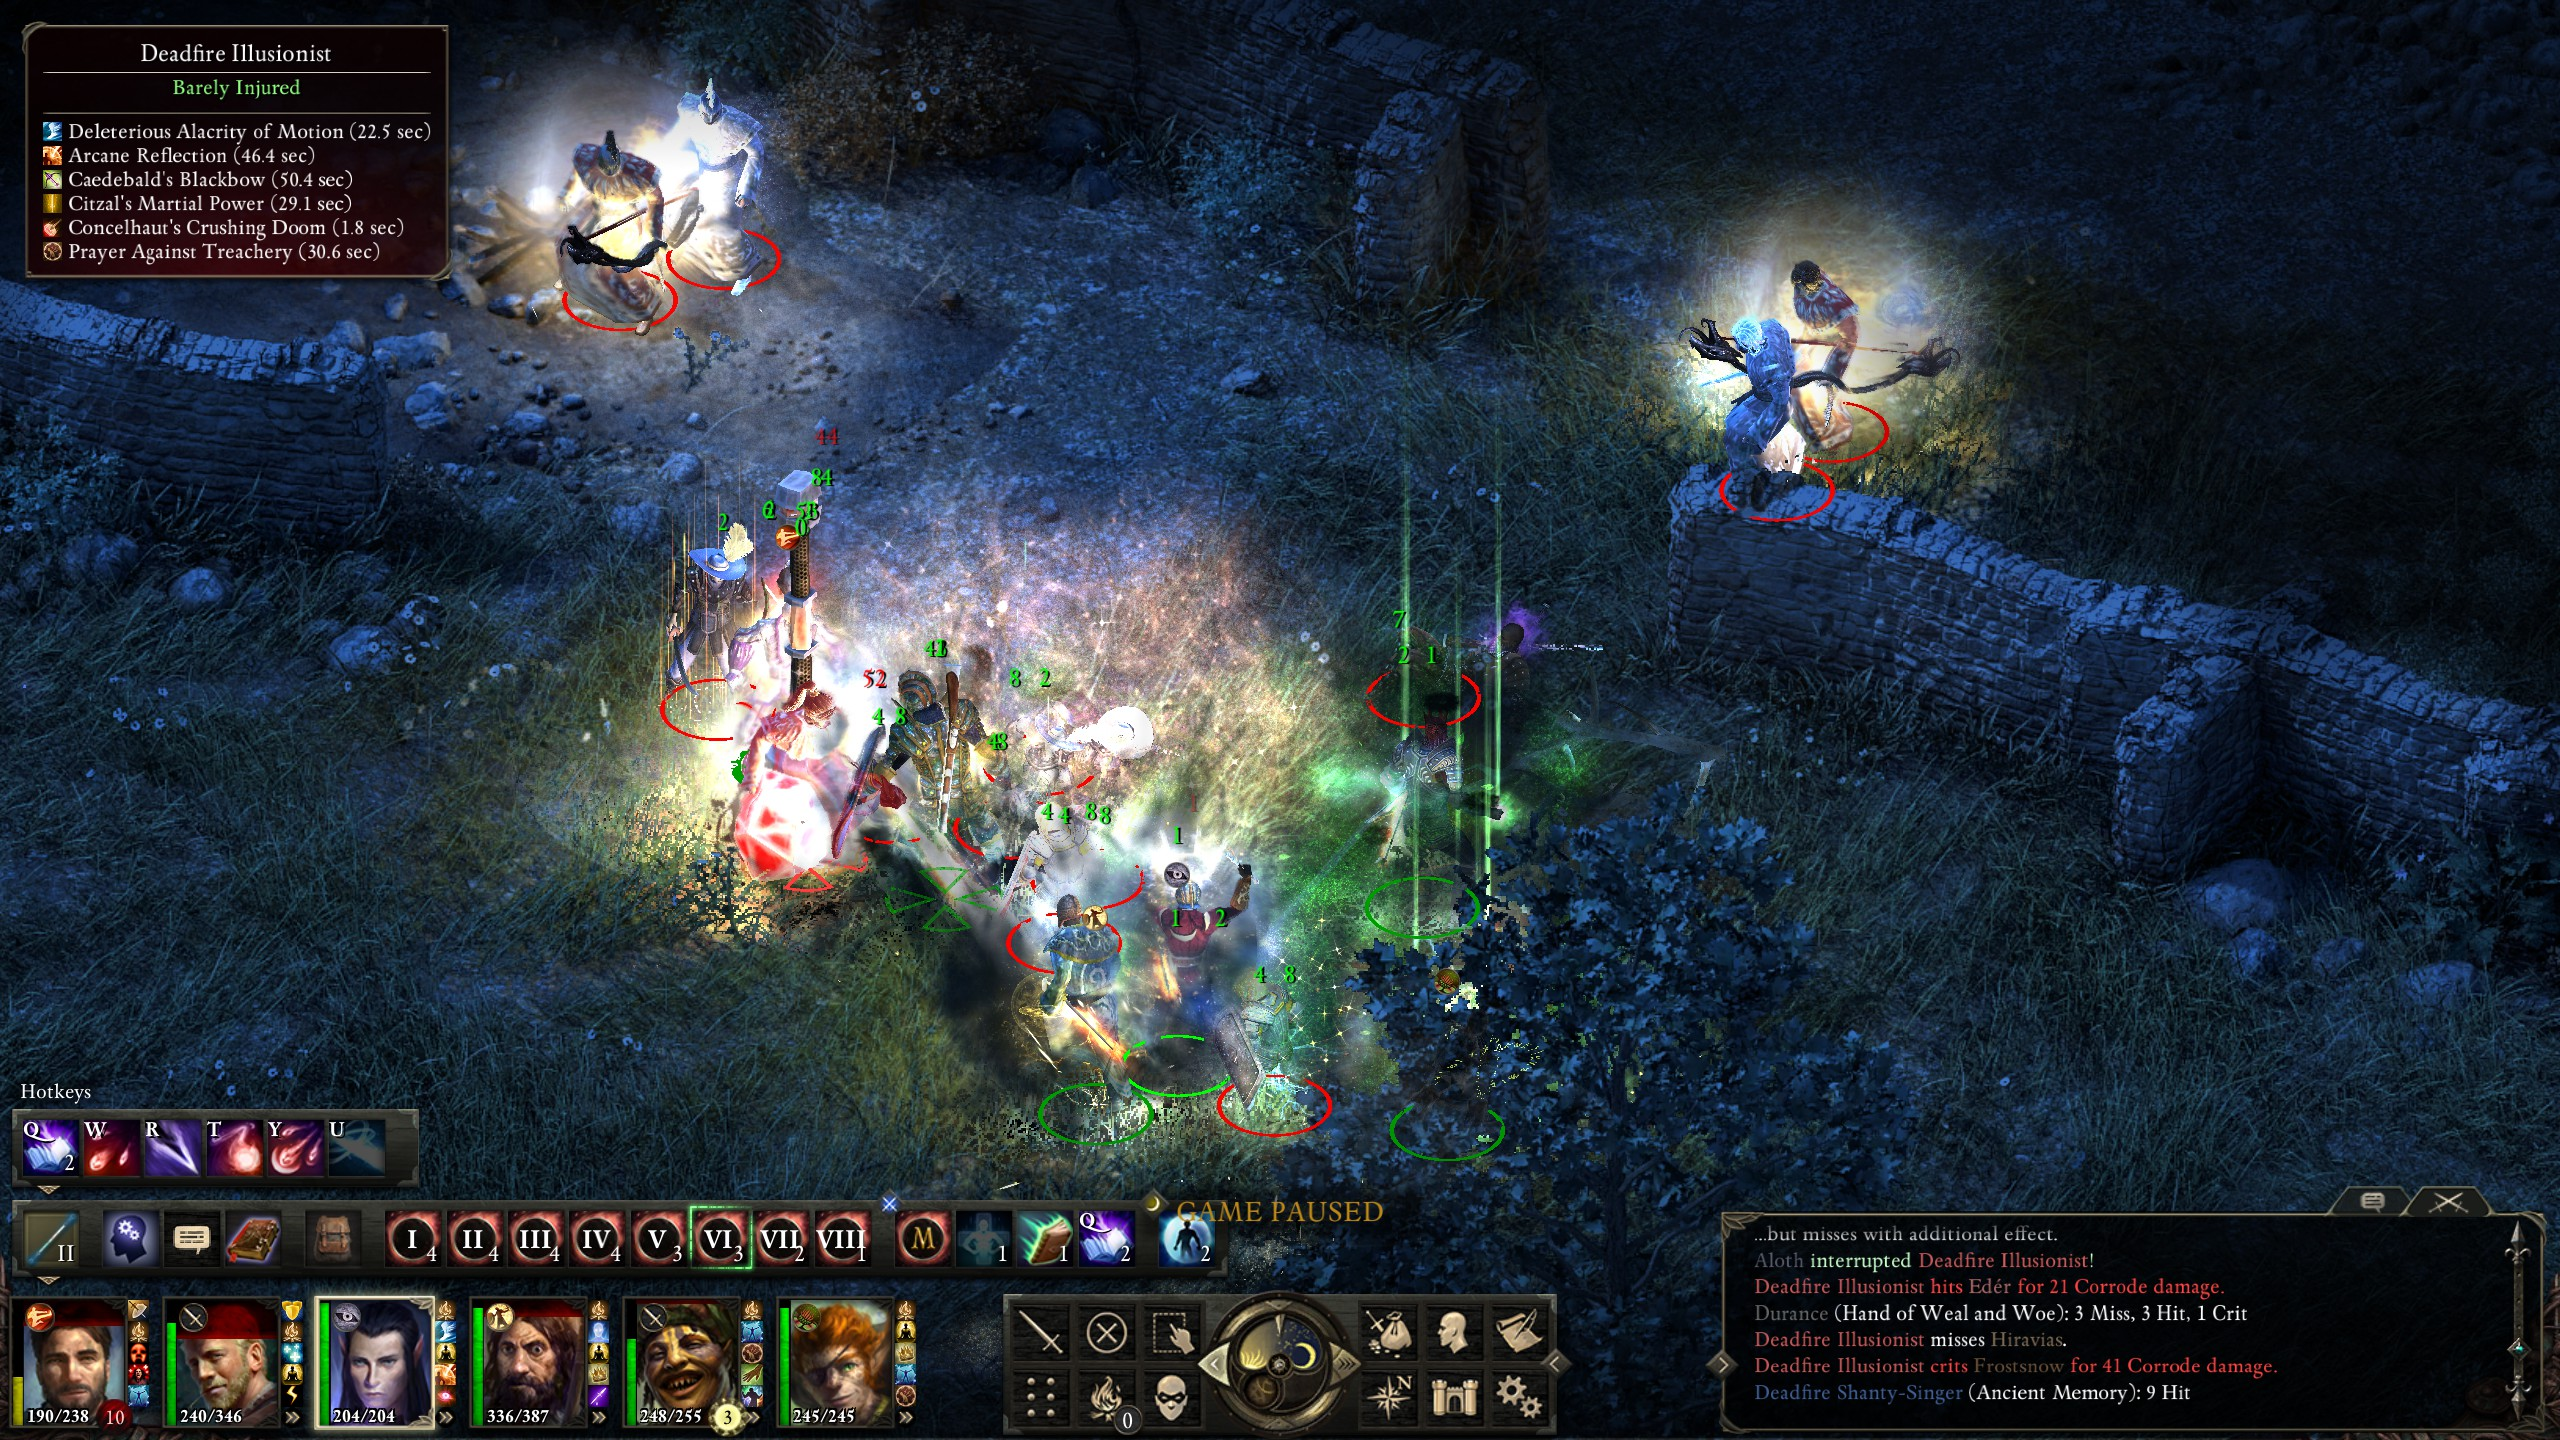
\includegraphics[scale=0.33]{files/blog/2020_01_18_poe_potd_wmpt2/2020_01_18_bounty4_2.jpg}
\end{figure}

Unfortunately for me, I made a few mistakes.  The first was to misremember the blackbow spell as doing raw damage when it actually did corrode, and the second was to use ``Flagellant's Path'' on the mage and thus leave my group before Hiravias's ``Weather the Storm'' buff had landed.  My monk then both took so much damage and wasn't able to deliver much due to the constant interruptions from being hit by arrows that he had to run back into the group so Durance could cast ``Barring Death's Door'' on my monk.

\begin{figure}
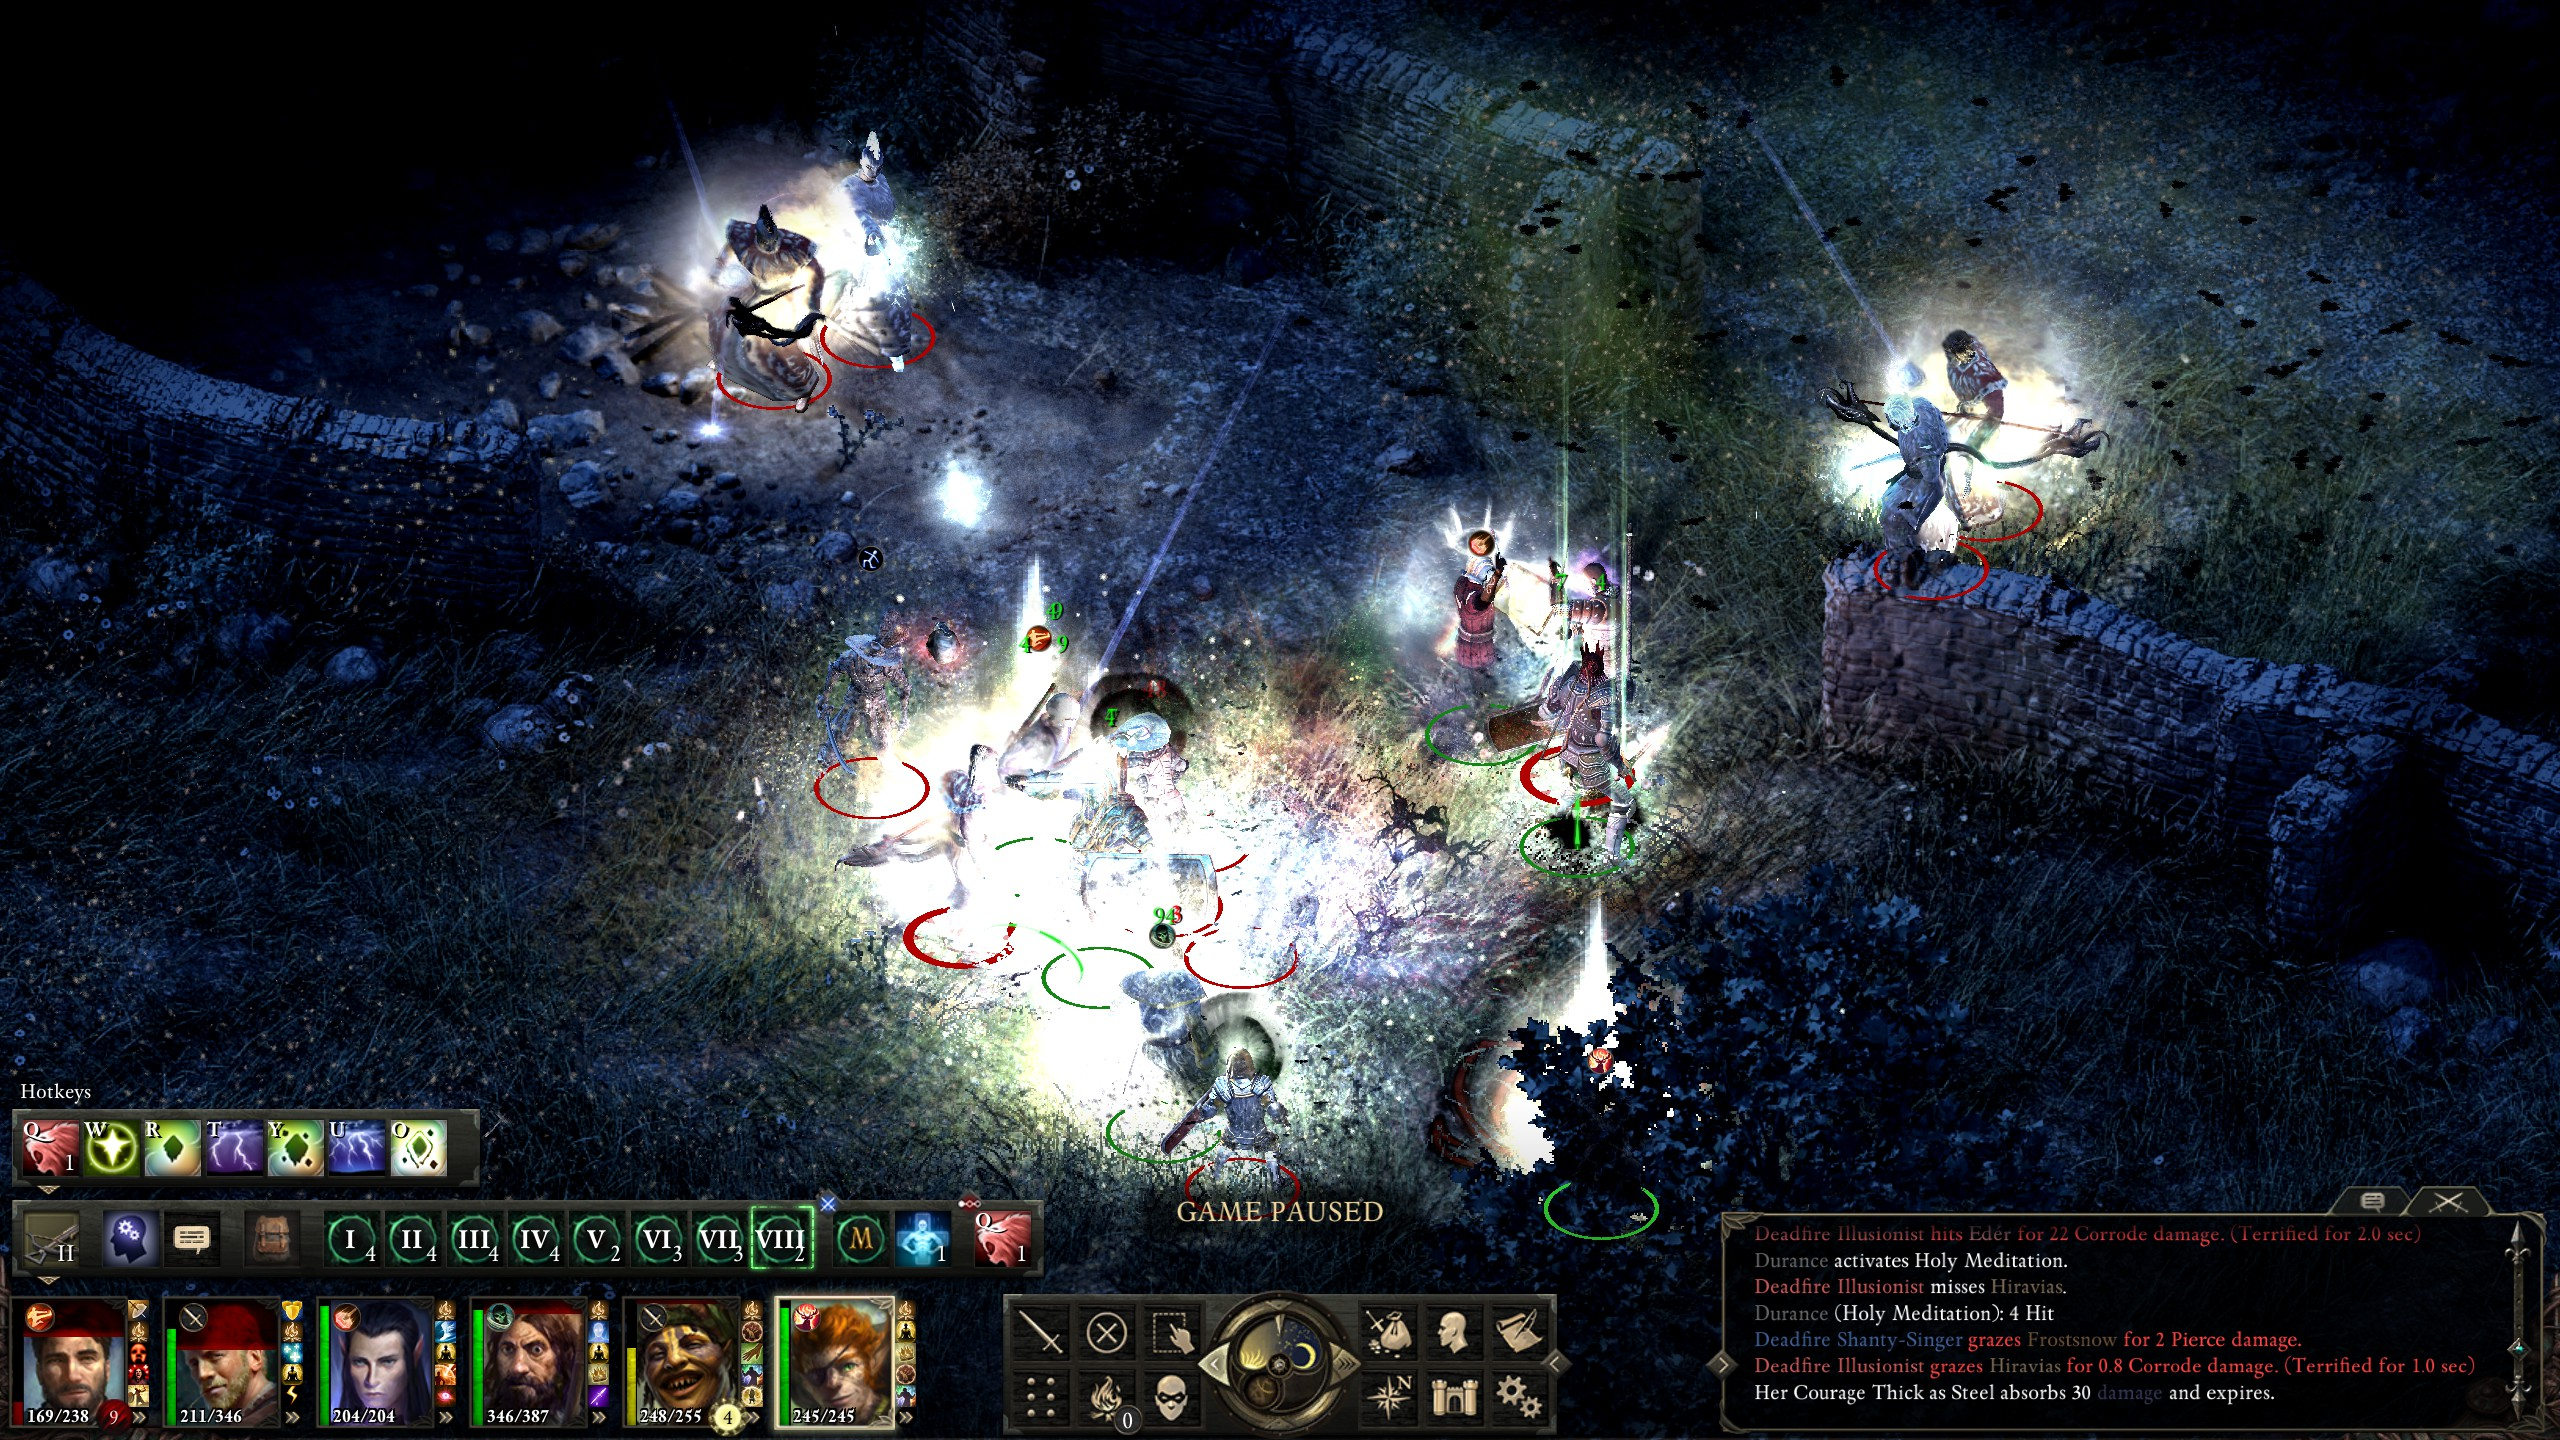
\includegraphics[scale=0.33]{files/blog/2020_01_18_poe_potd_wmpt2/2020_01_18_bounty4_3.jpg}
\end{figure}

It was a good thing, too, as my monk quickly ran out of health.  In the meantime I sent a few summoned creatures after the illusionists and had Aloth throw ``Concelhaut's Crushing Doom'' on each in order to hopefully disable them for a while.

\begin{figure}
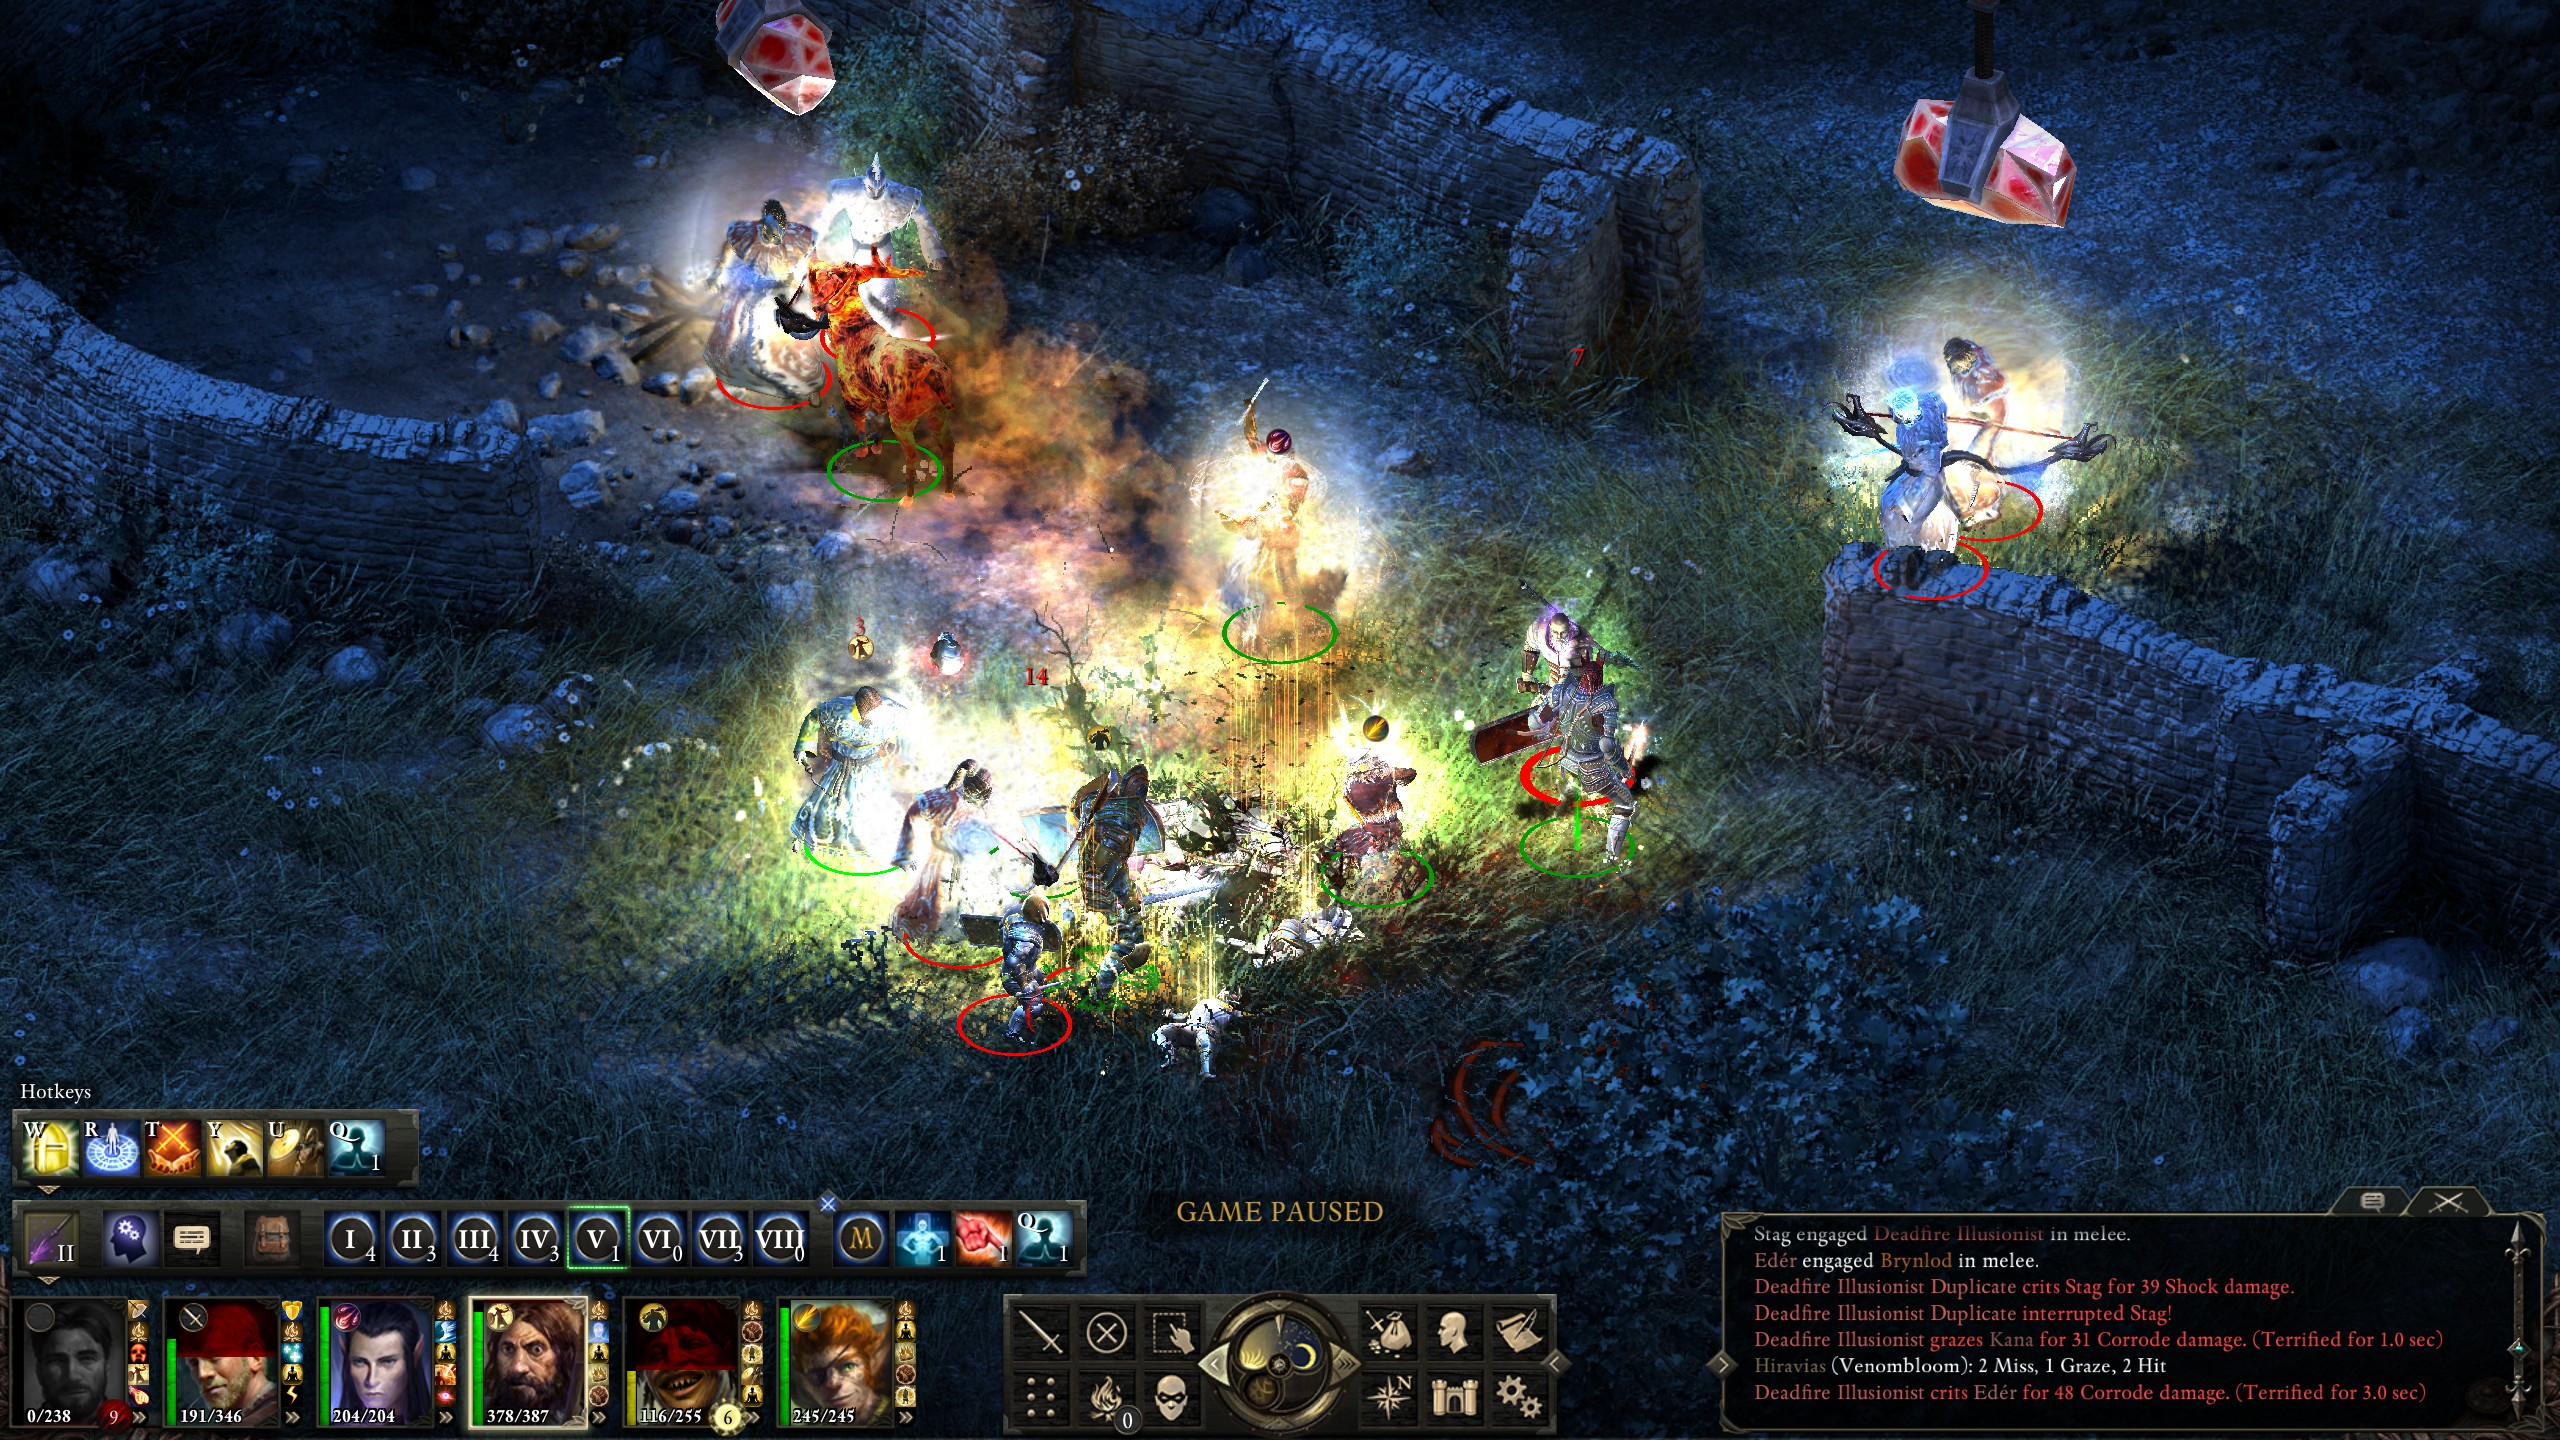
\includegraphics[scale=0.33]{files/blog/2020_01_18_poe_potd_wmpt2/2020_01_18_bounty4_4.jpg}
\end{figure}

Thanks to the sheer amount of buffs I had in my main group, such as ``Spark the Souls of the Righteous'', I eventually managed to kill the enemies around my main group, leaving only the outlying illusionists.

\begin{figure}
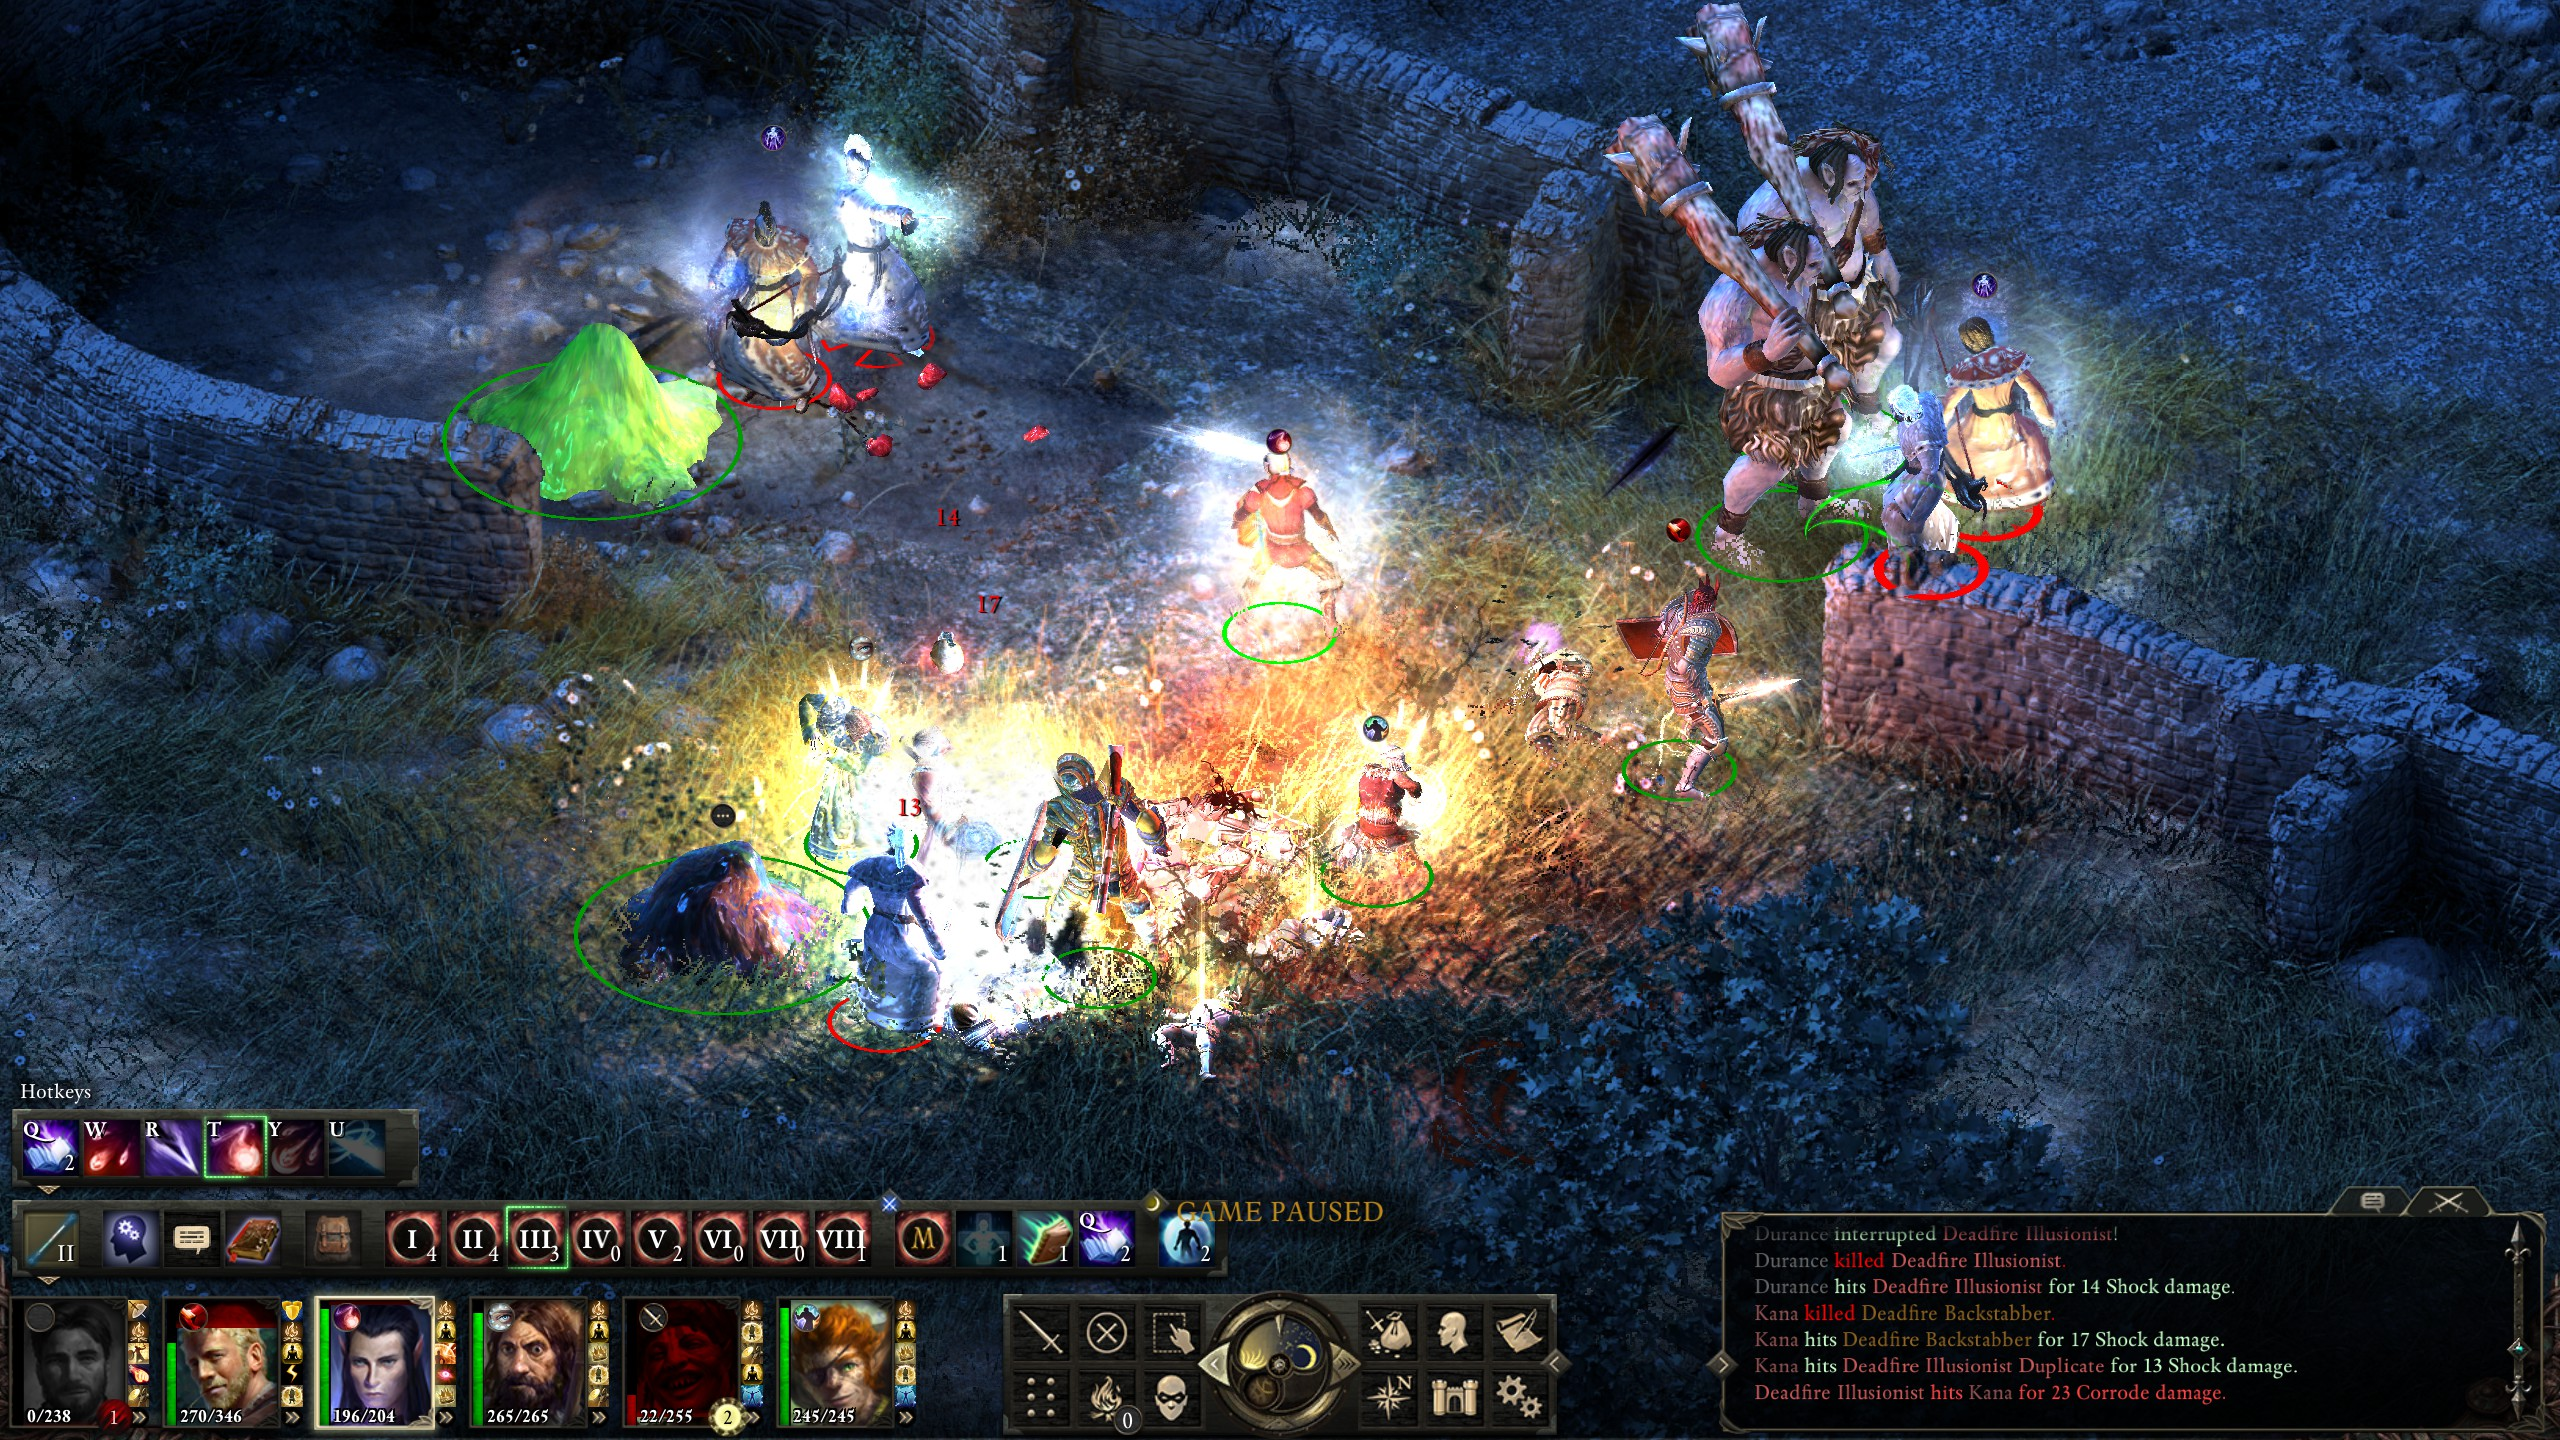
\includegraphics[scale=0.33]{files/blog/2020_01_18_poe_potd_wmpt2/2020_01_18_bounty4_5.jpg}
\end{figure}

At this point the battle had gone on long enough that the illusionists' buffs started to wear off and they had to re-cast a few of their spells.  Keeping as much elemental protection as I could muster up, I took my chance to kill them.

\begin{figure}
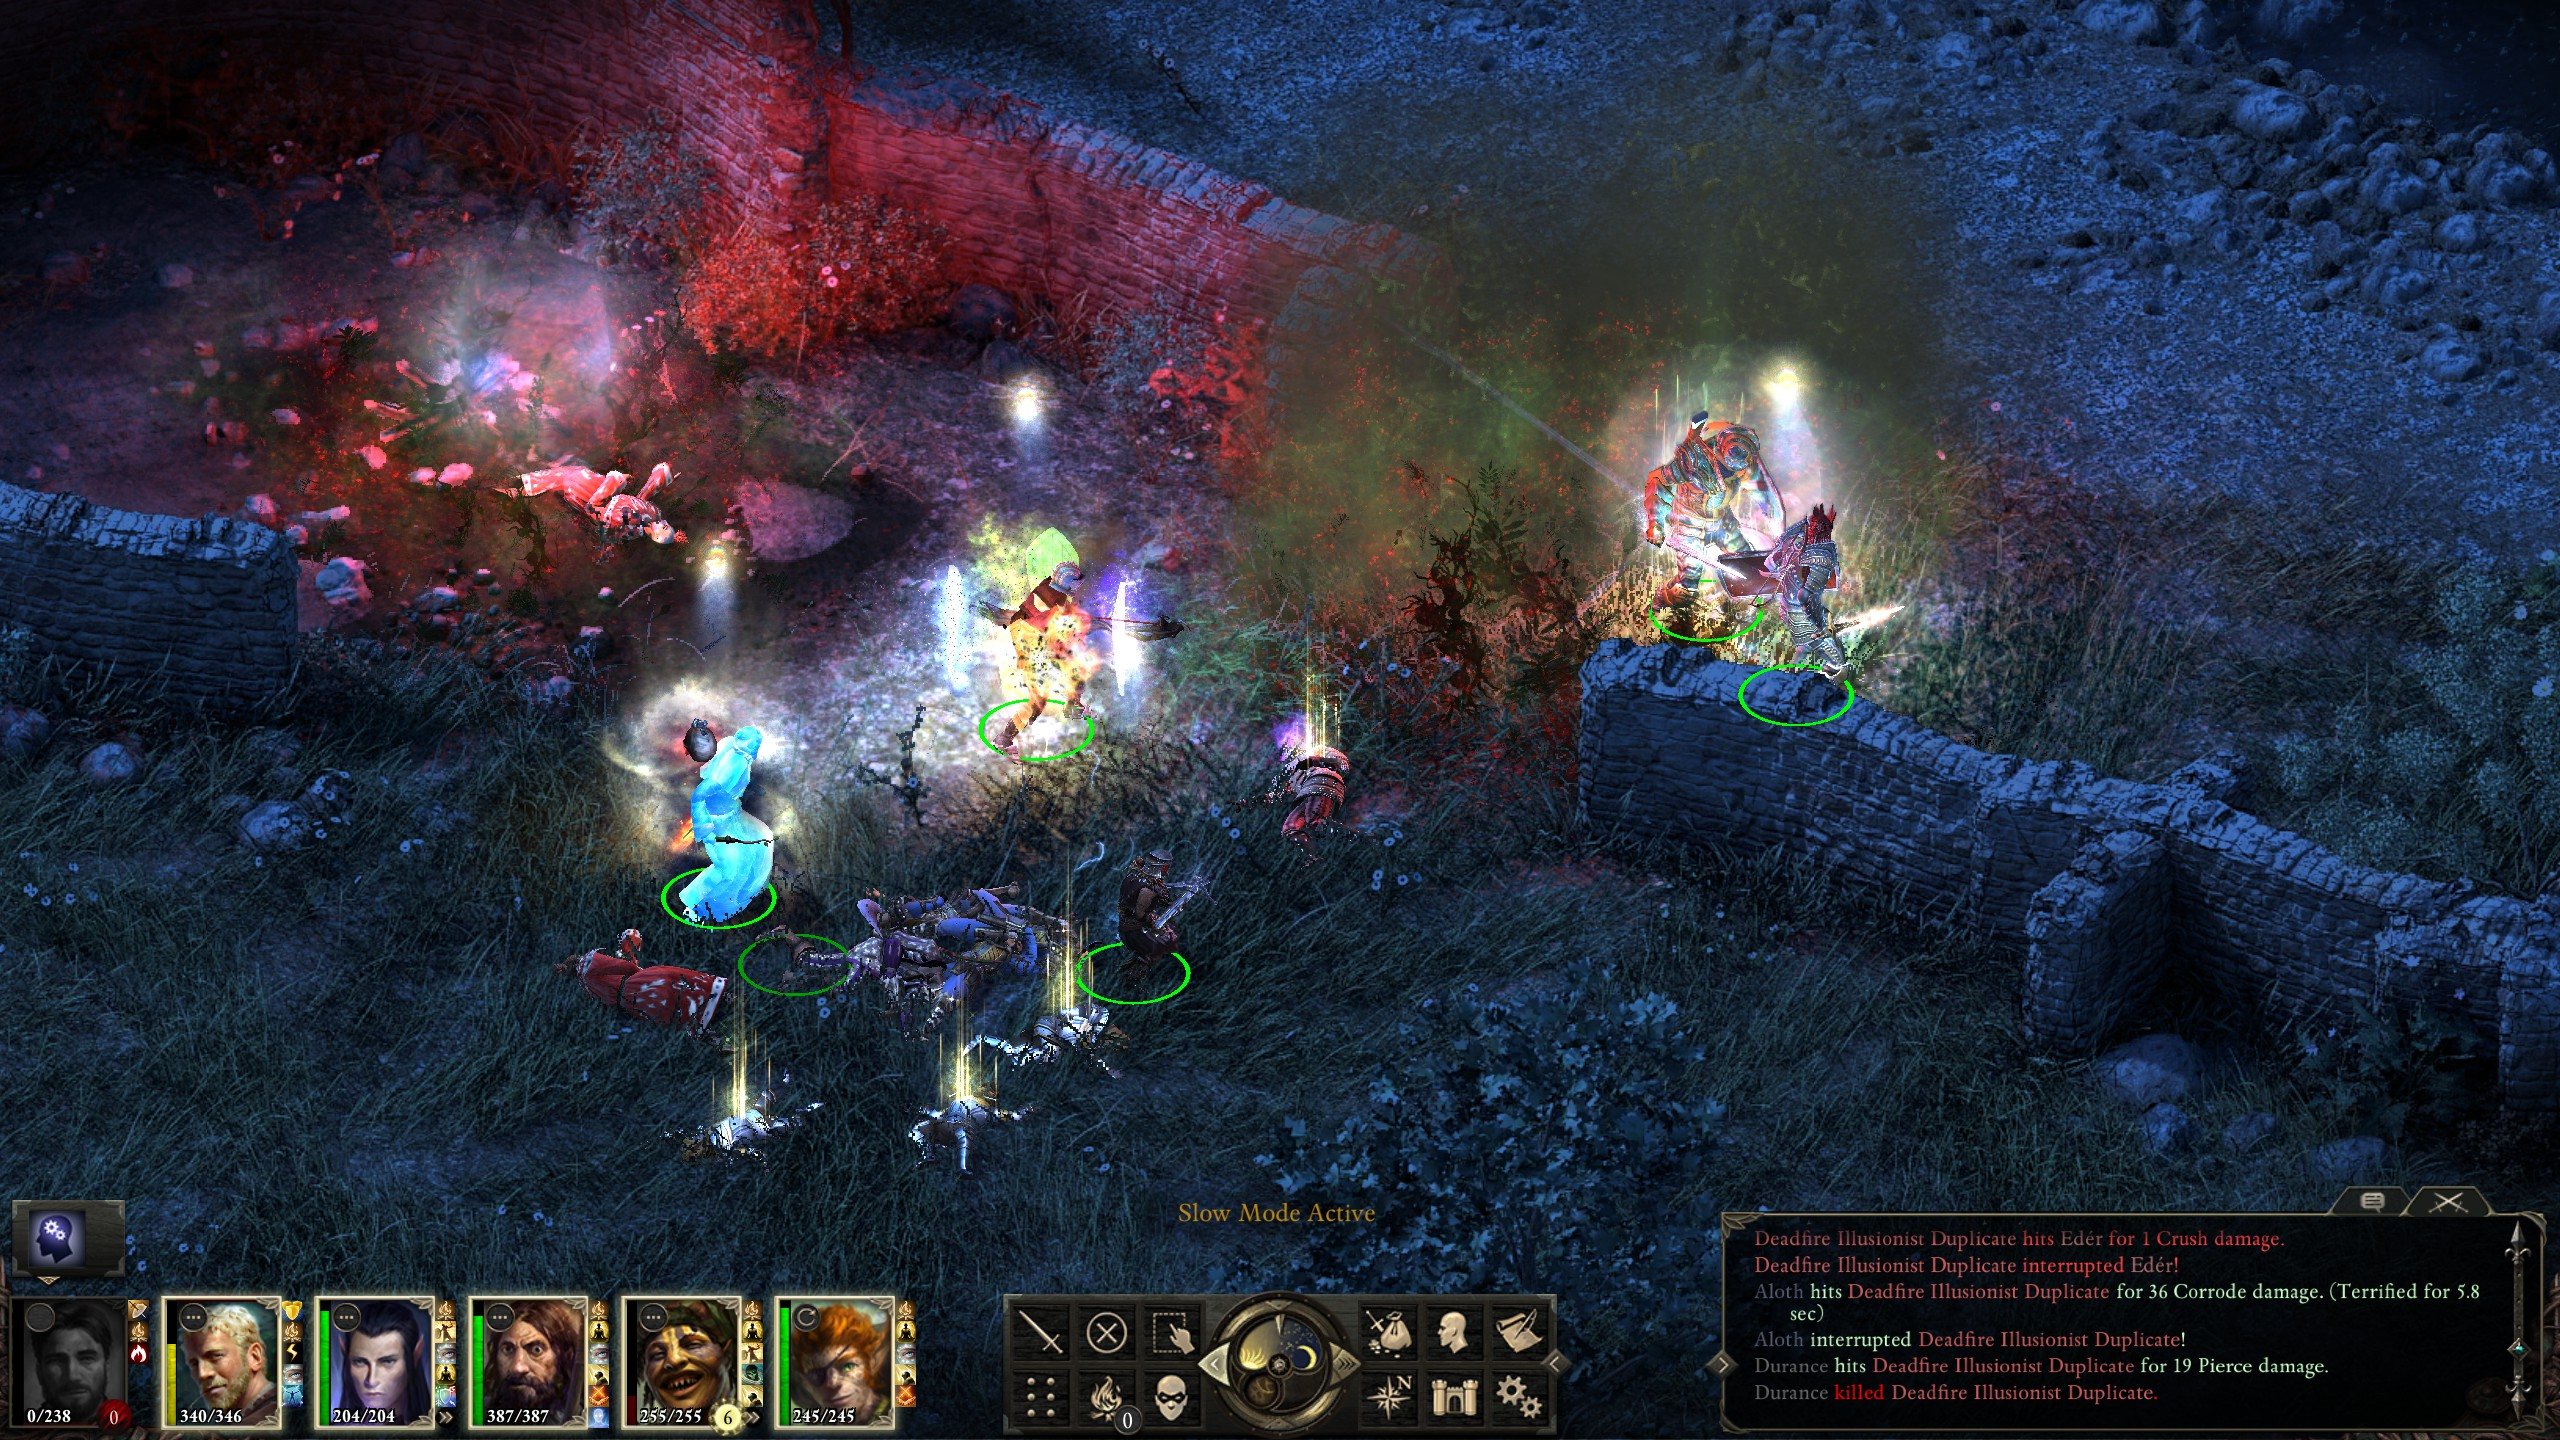
\includegraphics[scale=0.33]{files/blog/2020_01_18_poe_potd_wmpt2/2020_01_18_bounty4_6.jpg}
\end{figure}

More through sheer endurance than guile, I managed to recover from my mistakes and beat the pirates on first try, but it was a very close fight.  With the last bounty done, I headed to Iron Flail Fort in order to advance the main storyline.

\subsection{Iron Flail Fort}
Using the cannons that I had restored earlier, I took the fun entrance into the Iron Flail Fort by blasting the gate down and plowing through the guards.

\begin{figure}
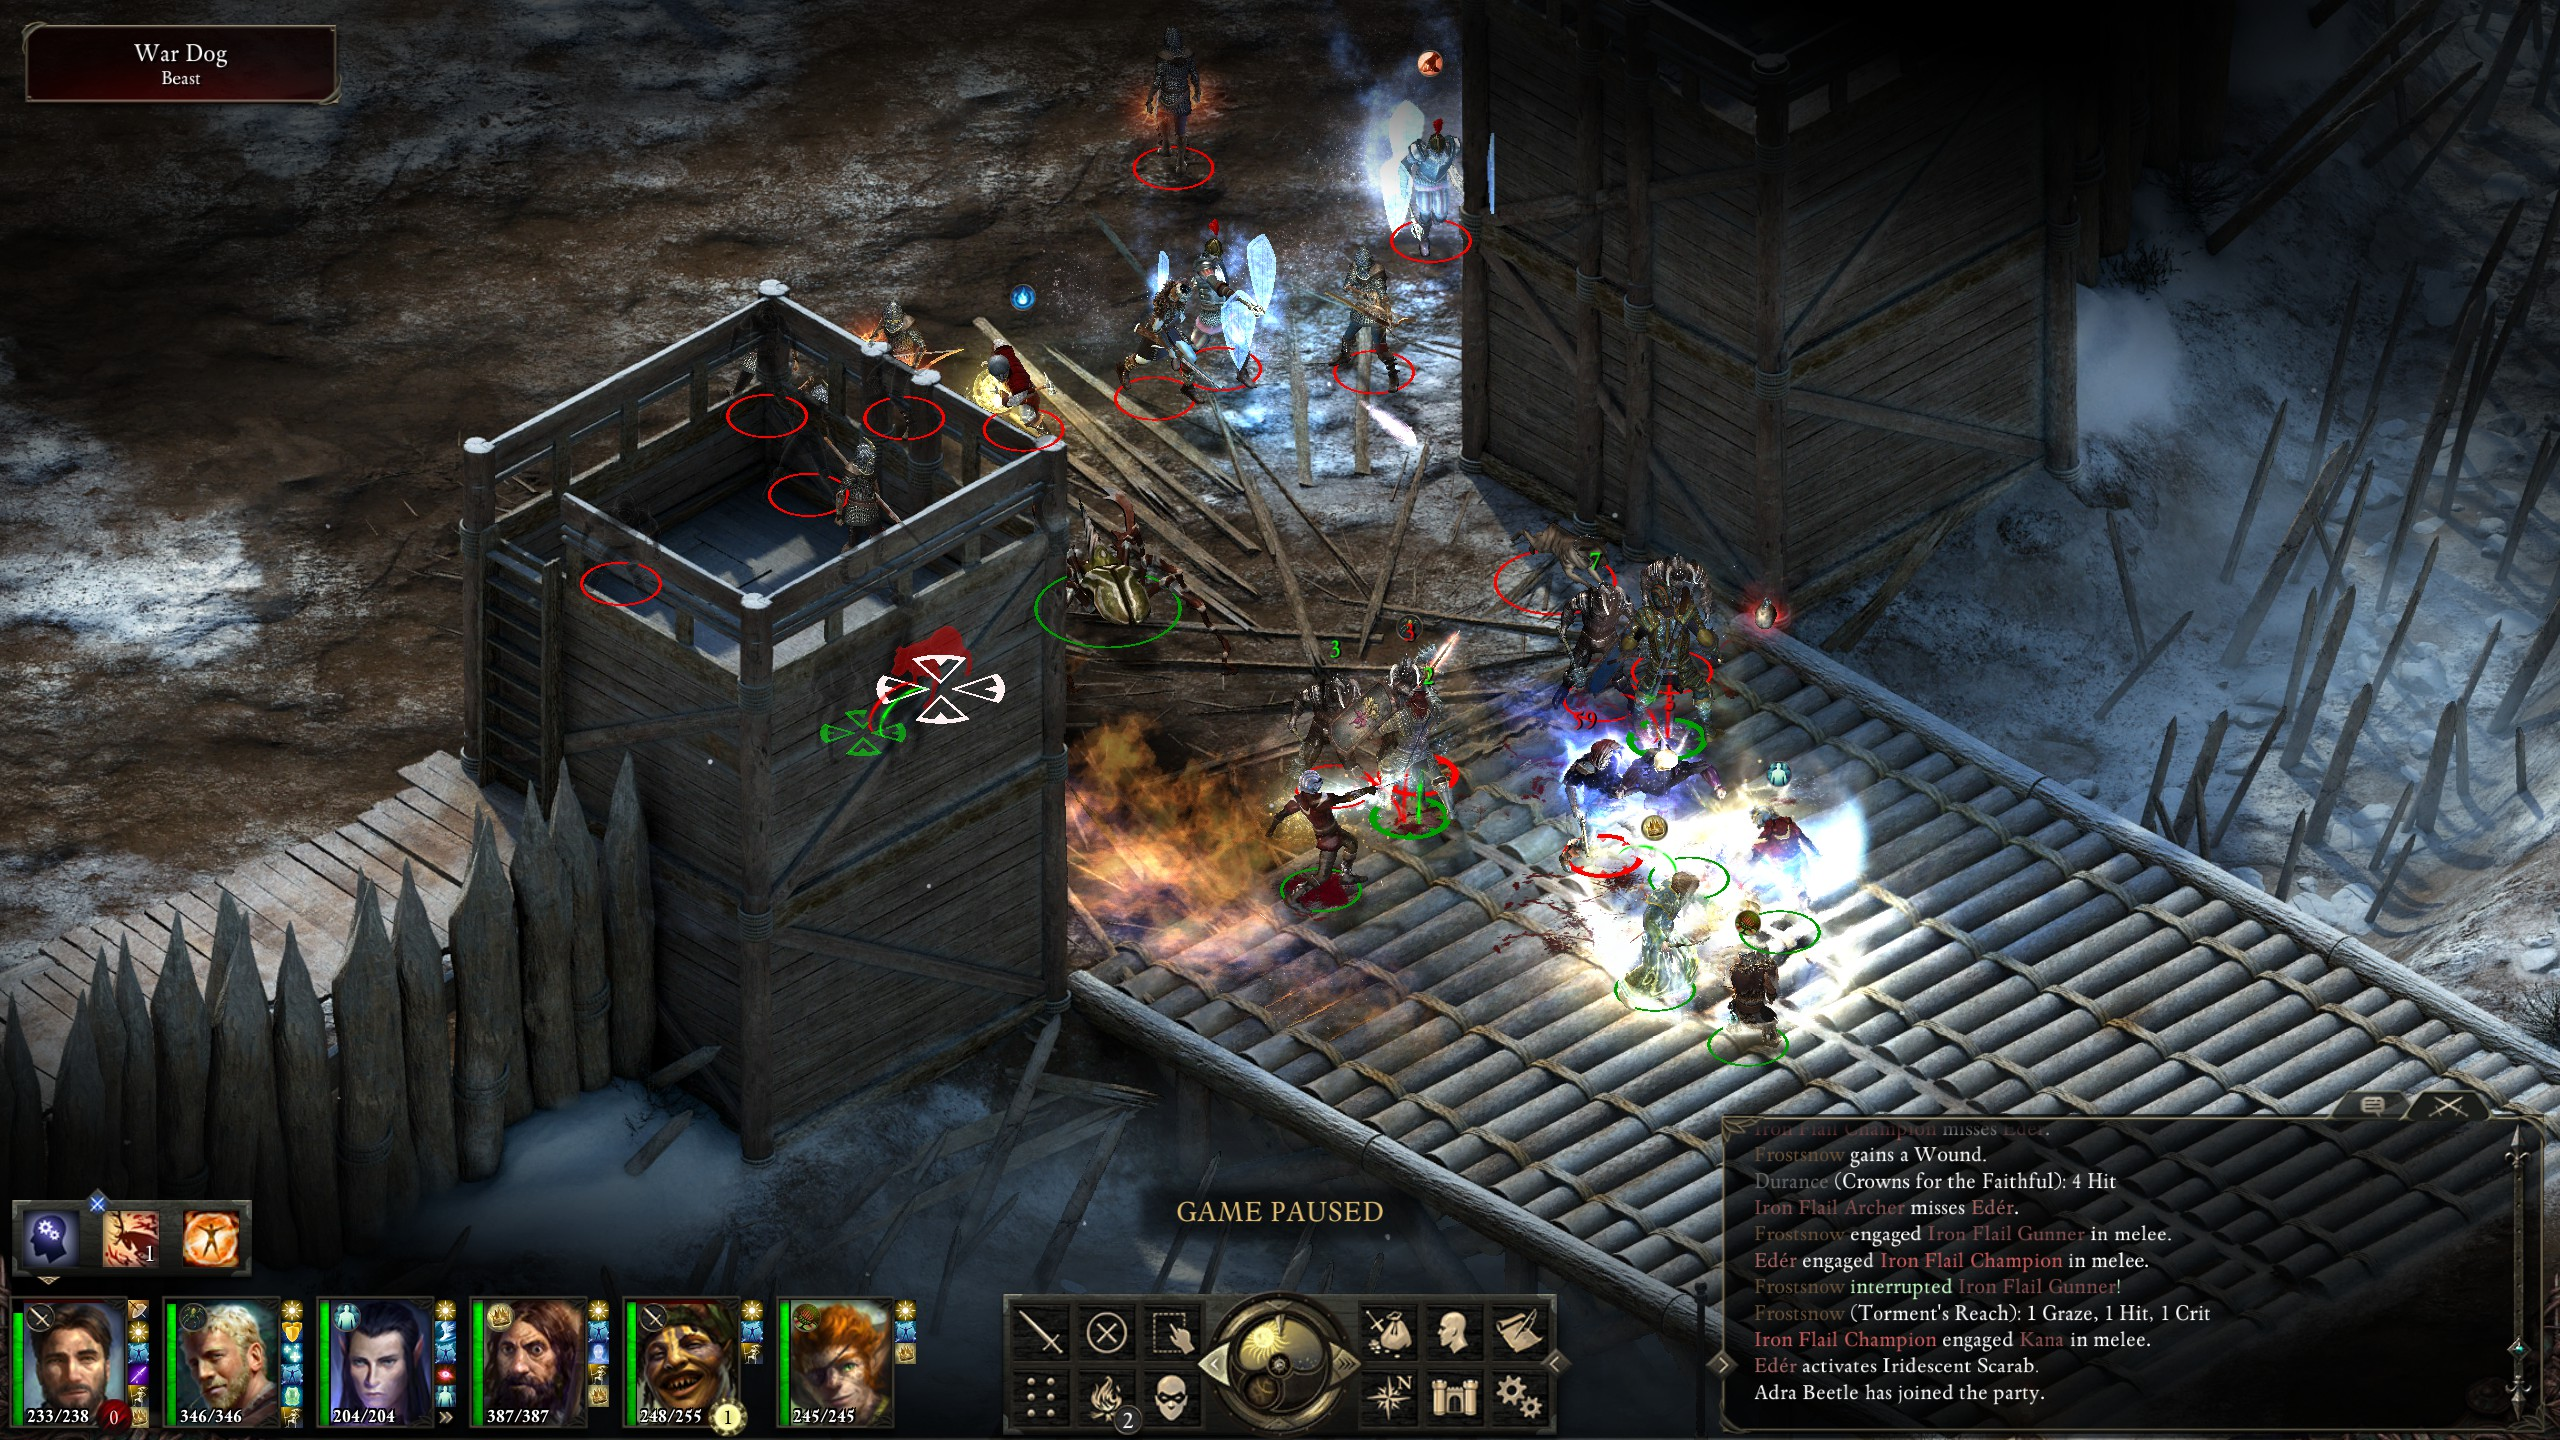
\includegraphics[scale=0.33]{files/blog/2020_01_18_poe_potd_wmpt2/2020_01_18_fort1.jpg}
\end{figure}

The guards didn't prove particularly difficult, and I made it to Adaryc without much problem.

\begin{figure}
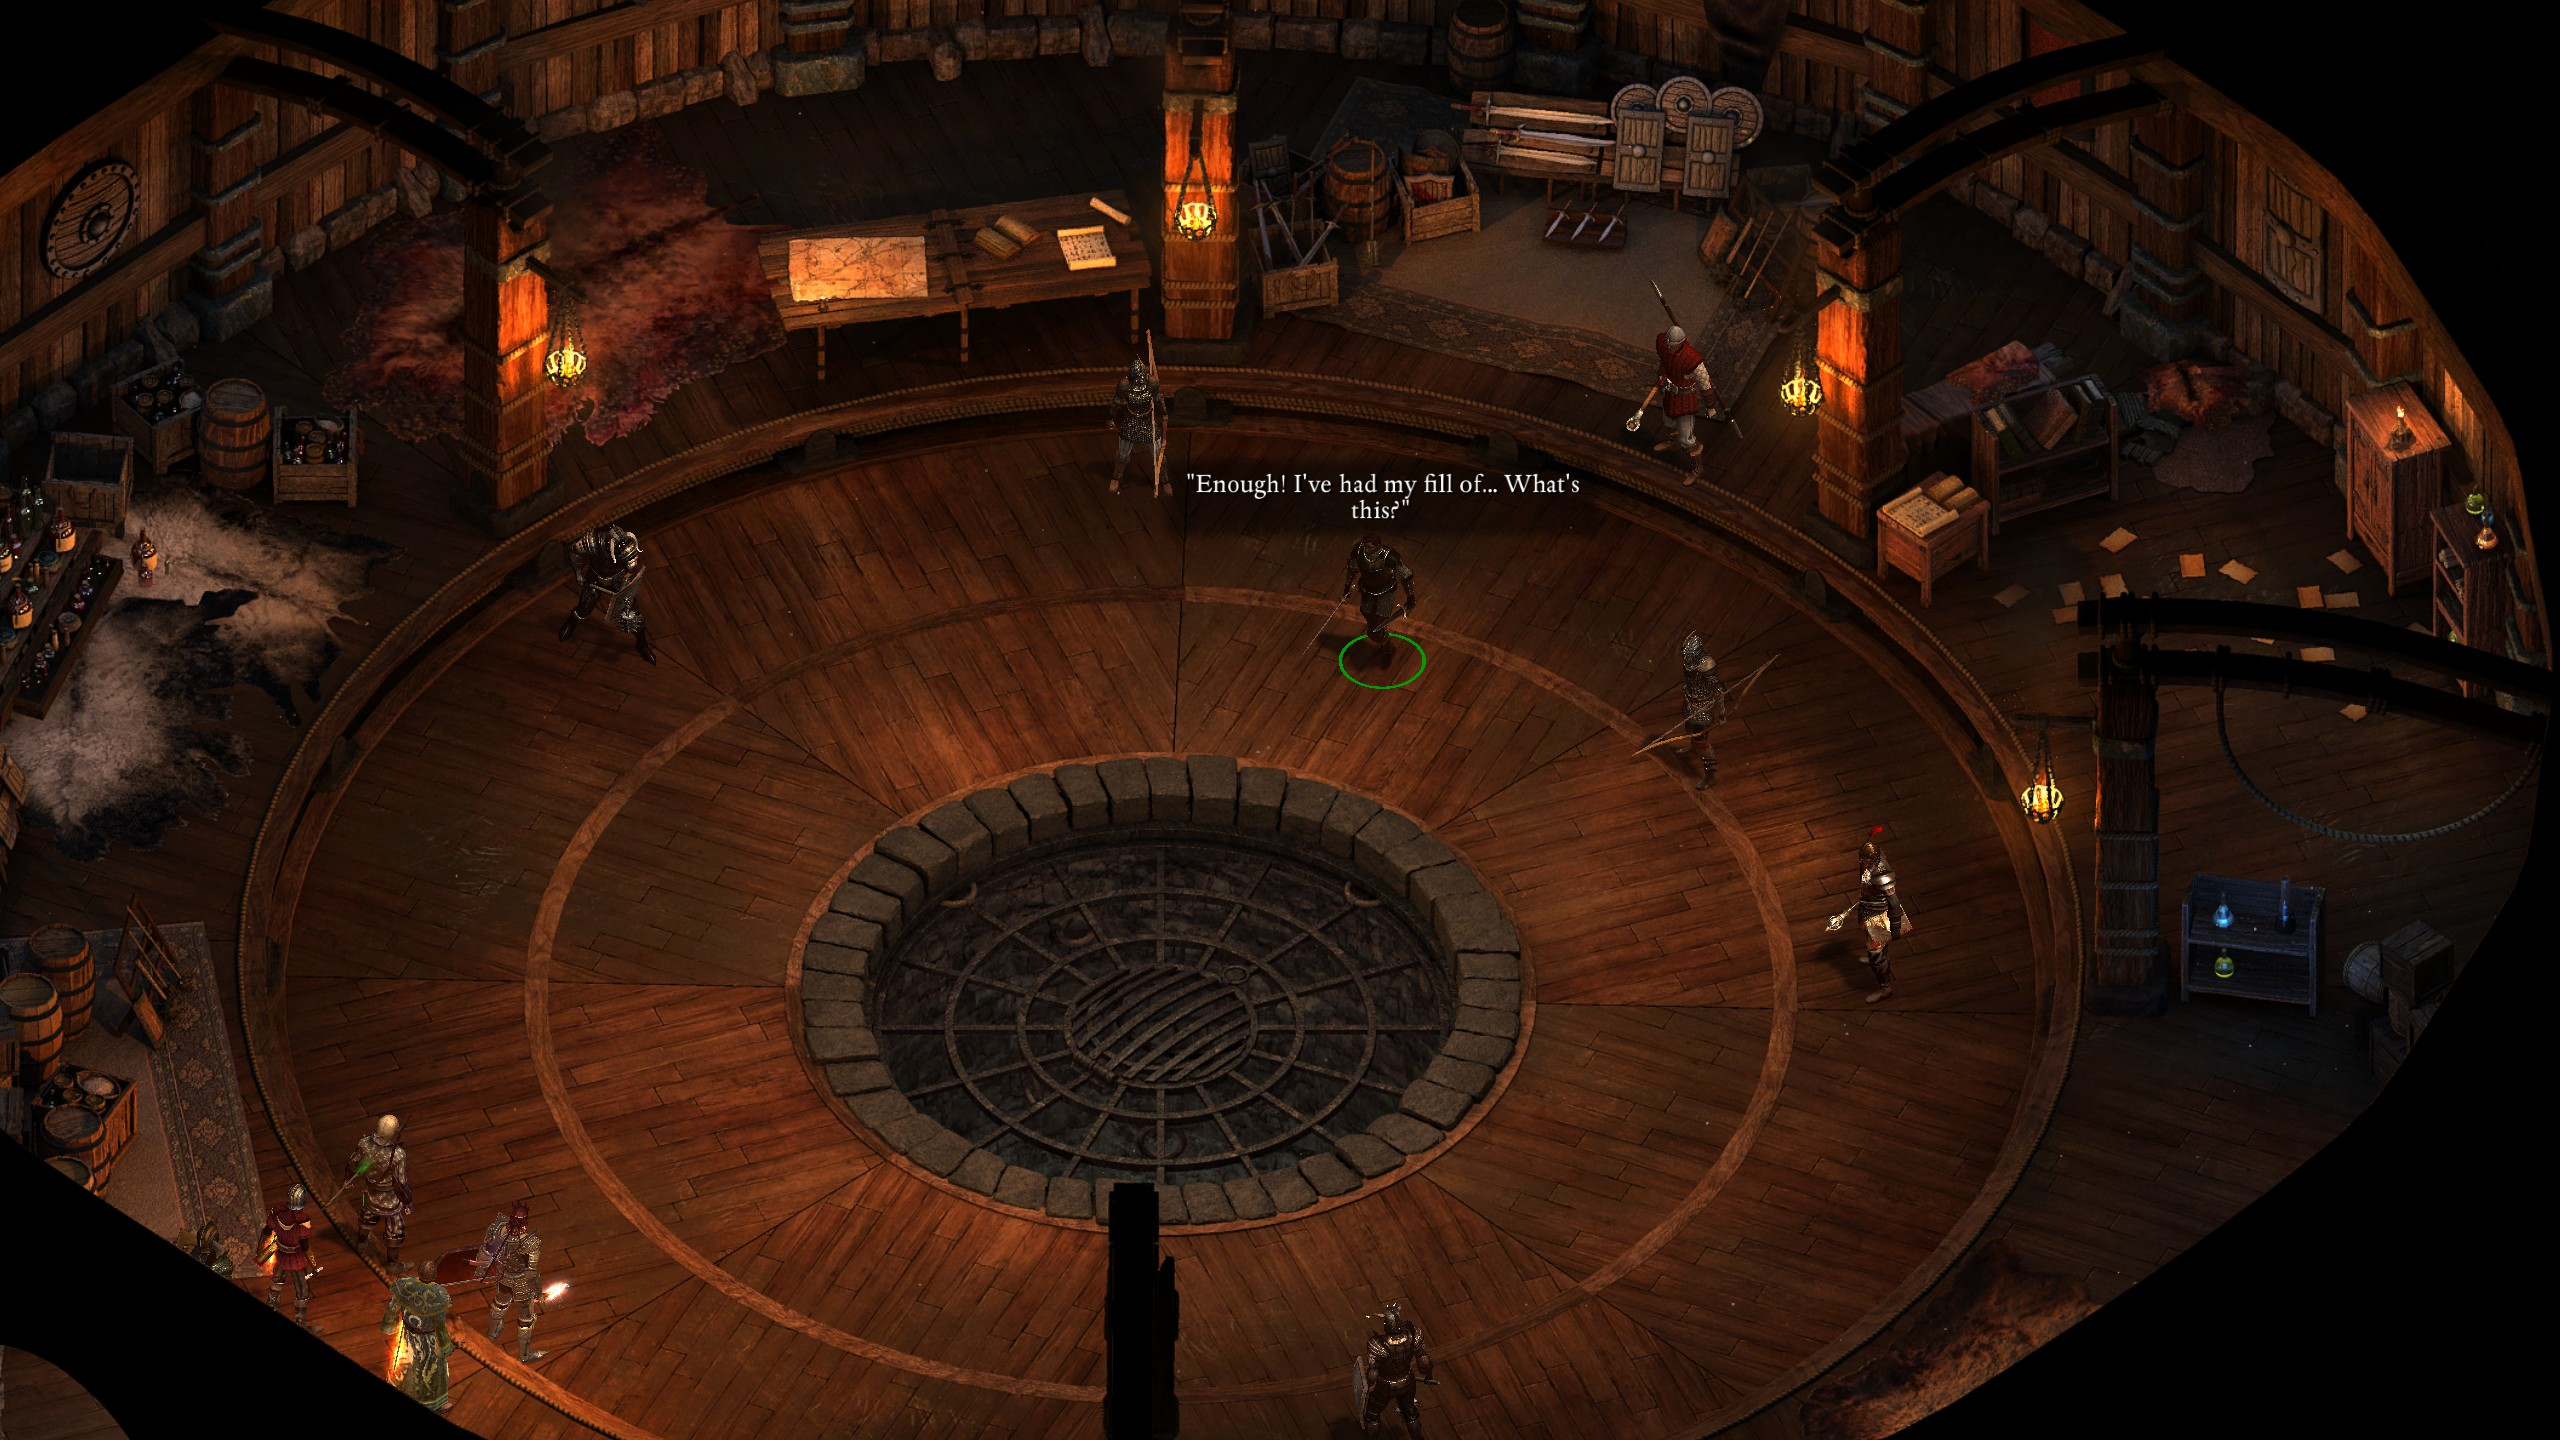
\includegraphics[scale=0.33]{files/blog/2020_01_18_poe_potd_wmpt2/2020_01_18_fort2.jpg}
\end{figure}

I managed to convince him to help me, but then, unfortunately, I forgot to take a screenshot of my battle with the eyeless afterwards, although the battle didn't prove difficult.  I used ``Concelhaut's Crushing Doom'' in order to disable them and then took them down one at a time using focus firing.  Once the eyeless were dead, I set out for the abbey.

\subsection{Abbey of the Fallen Moon}
Perhaps one of the prettiest areas in the game, the Abbey of the Fallen Moon had many good-looking areas worth showing off.  As for the fanatics, they tried to drive me away and failed, but we had some pretty good fights along the way.

\begin{figure}
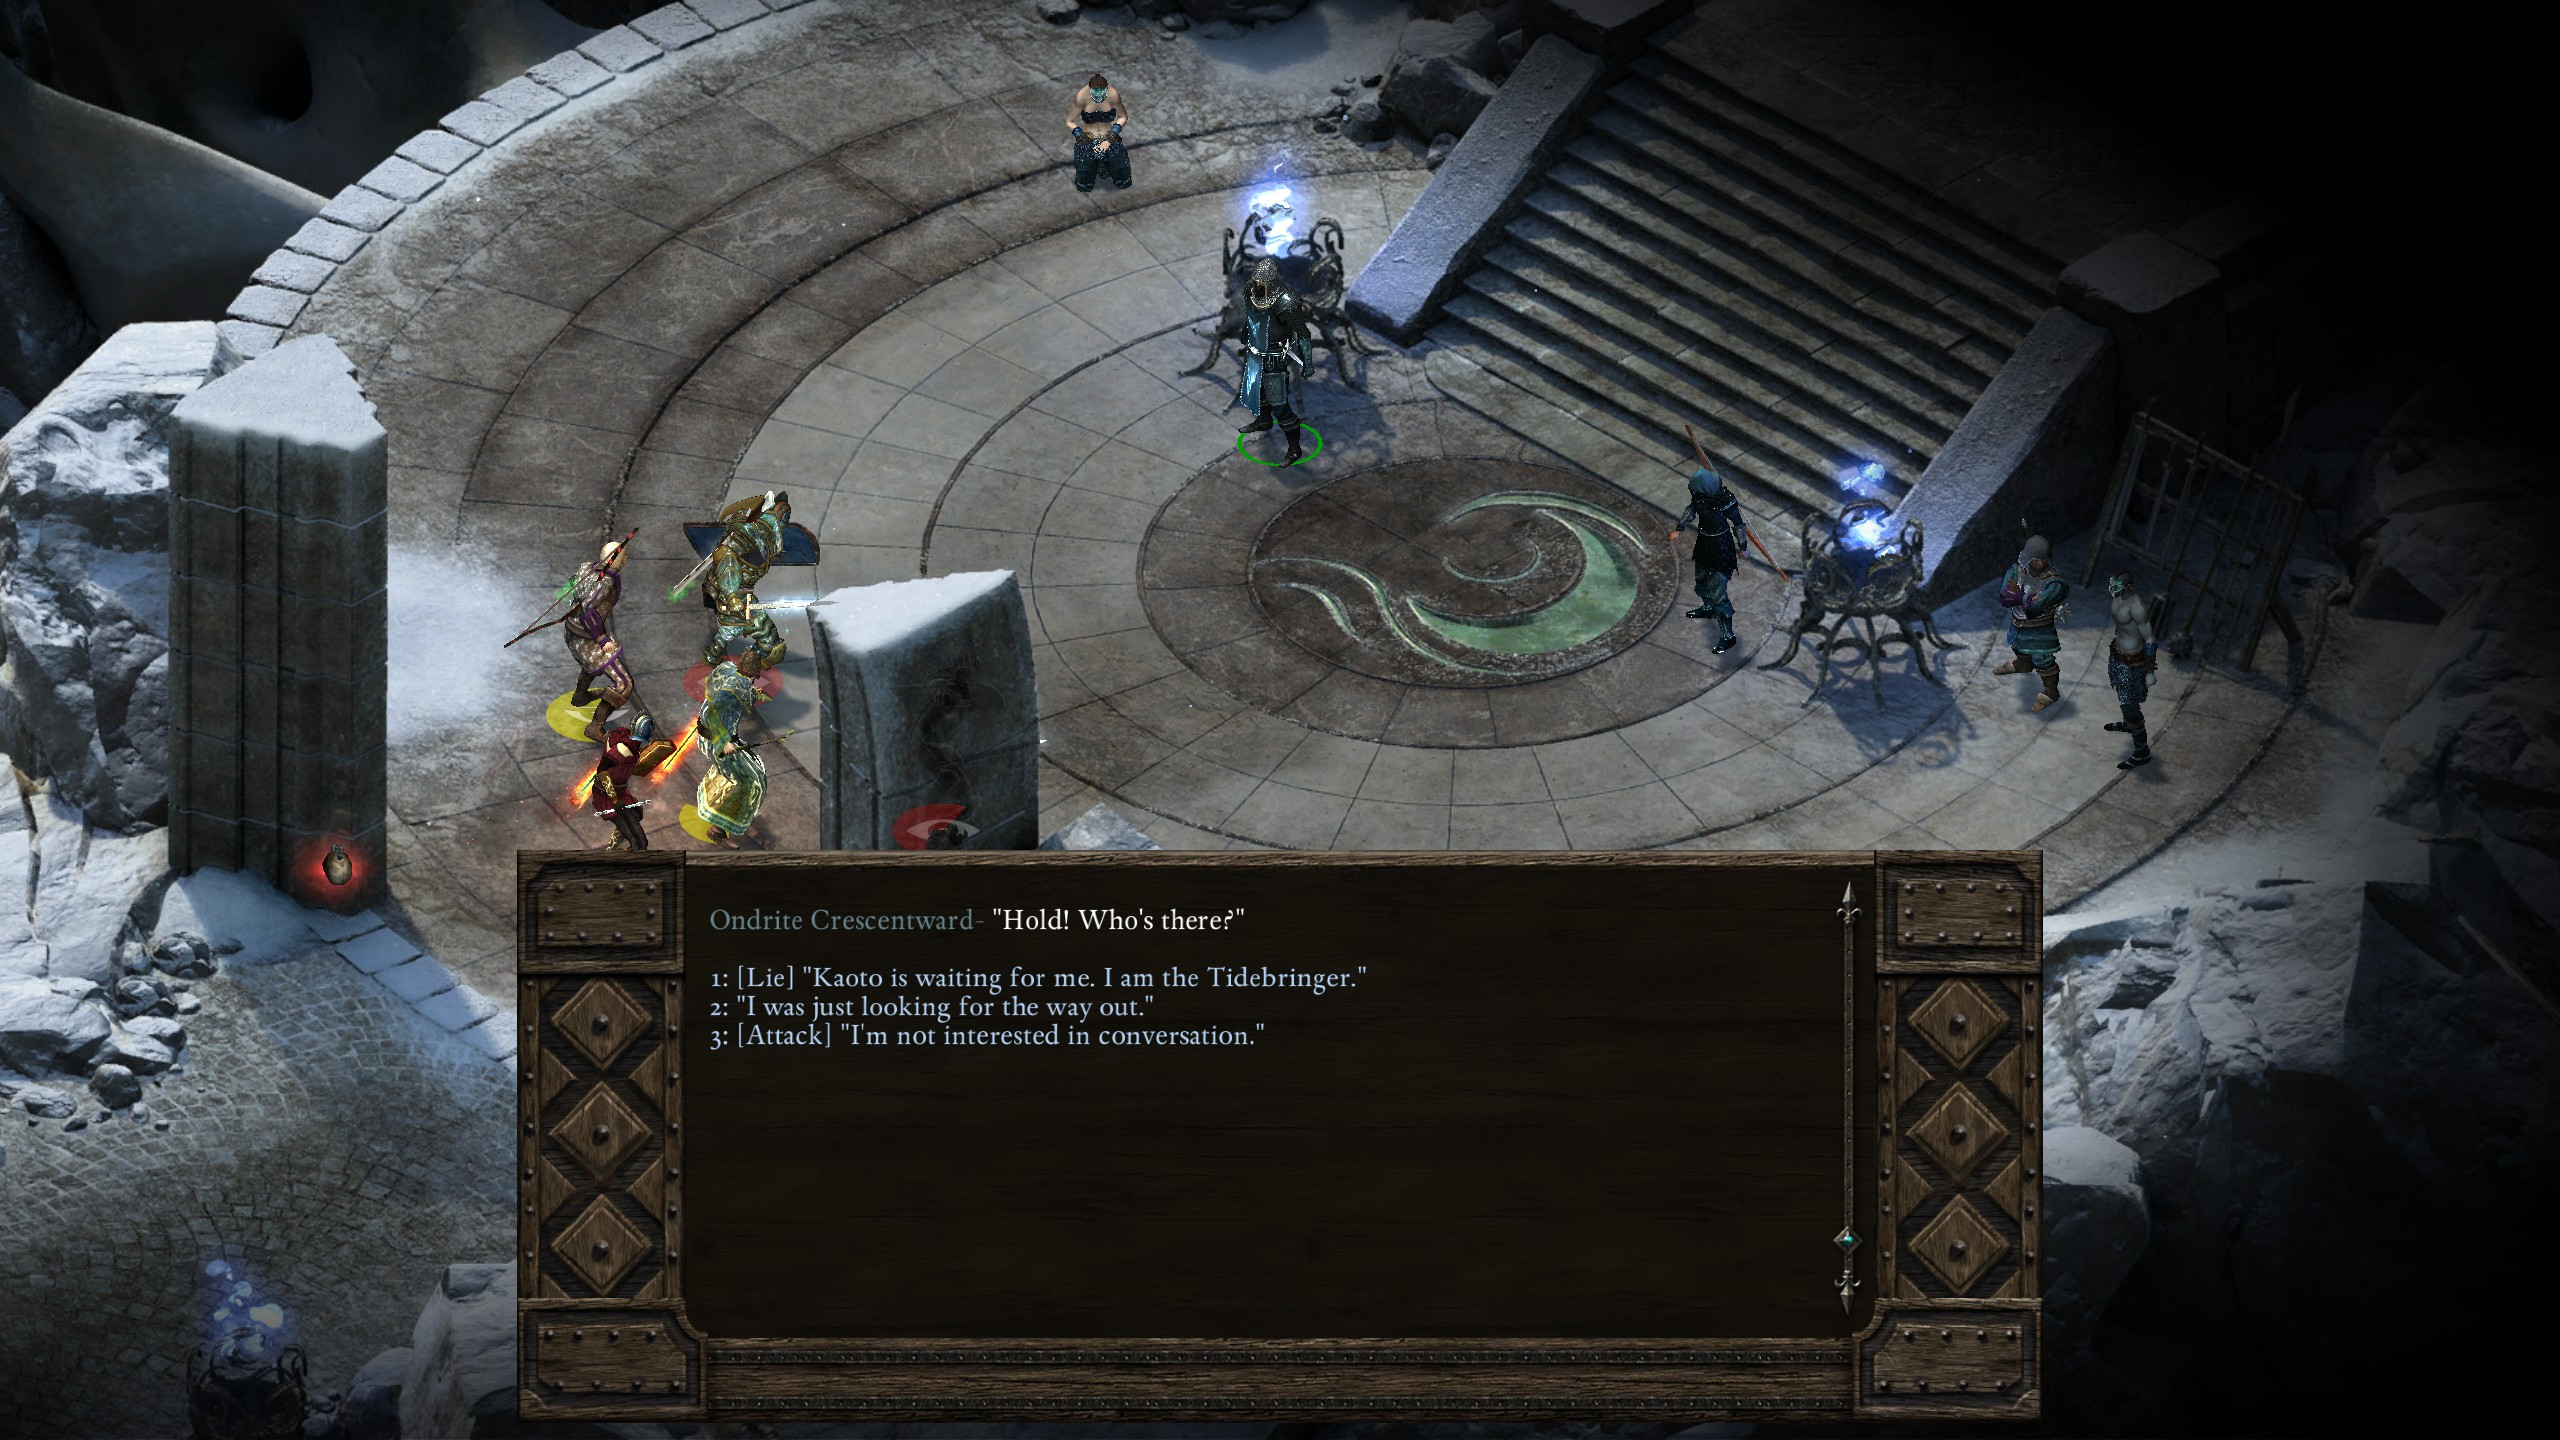
\includegraphics[scale=0.33]{files/blog/2020_01_18_poe_potd_wmpt2/2020_01_18_abbey01.jpg}
\end{figure}

The main entrance contained the ribcage of a giant skeleton in addition to a large number of guards and some ice blights that would spawn in the middle of the fight.

\begin{figure}
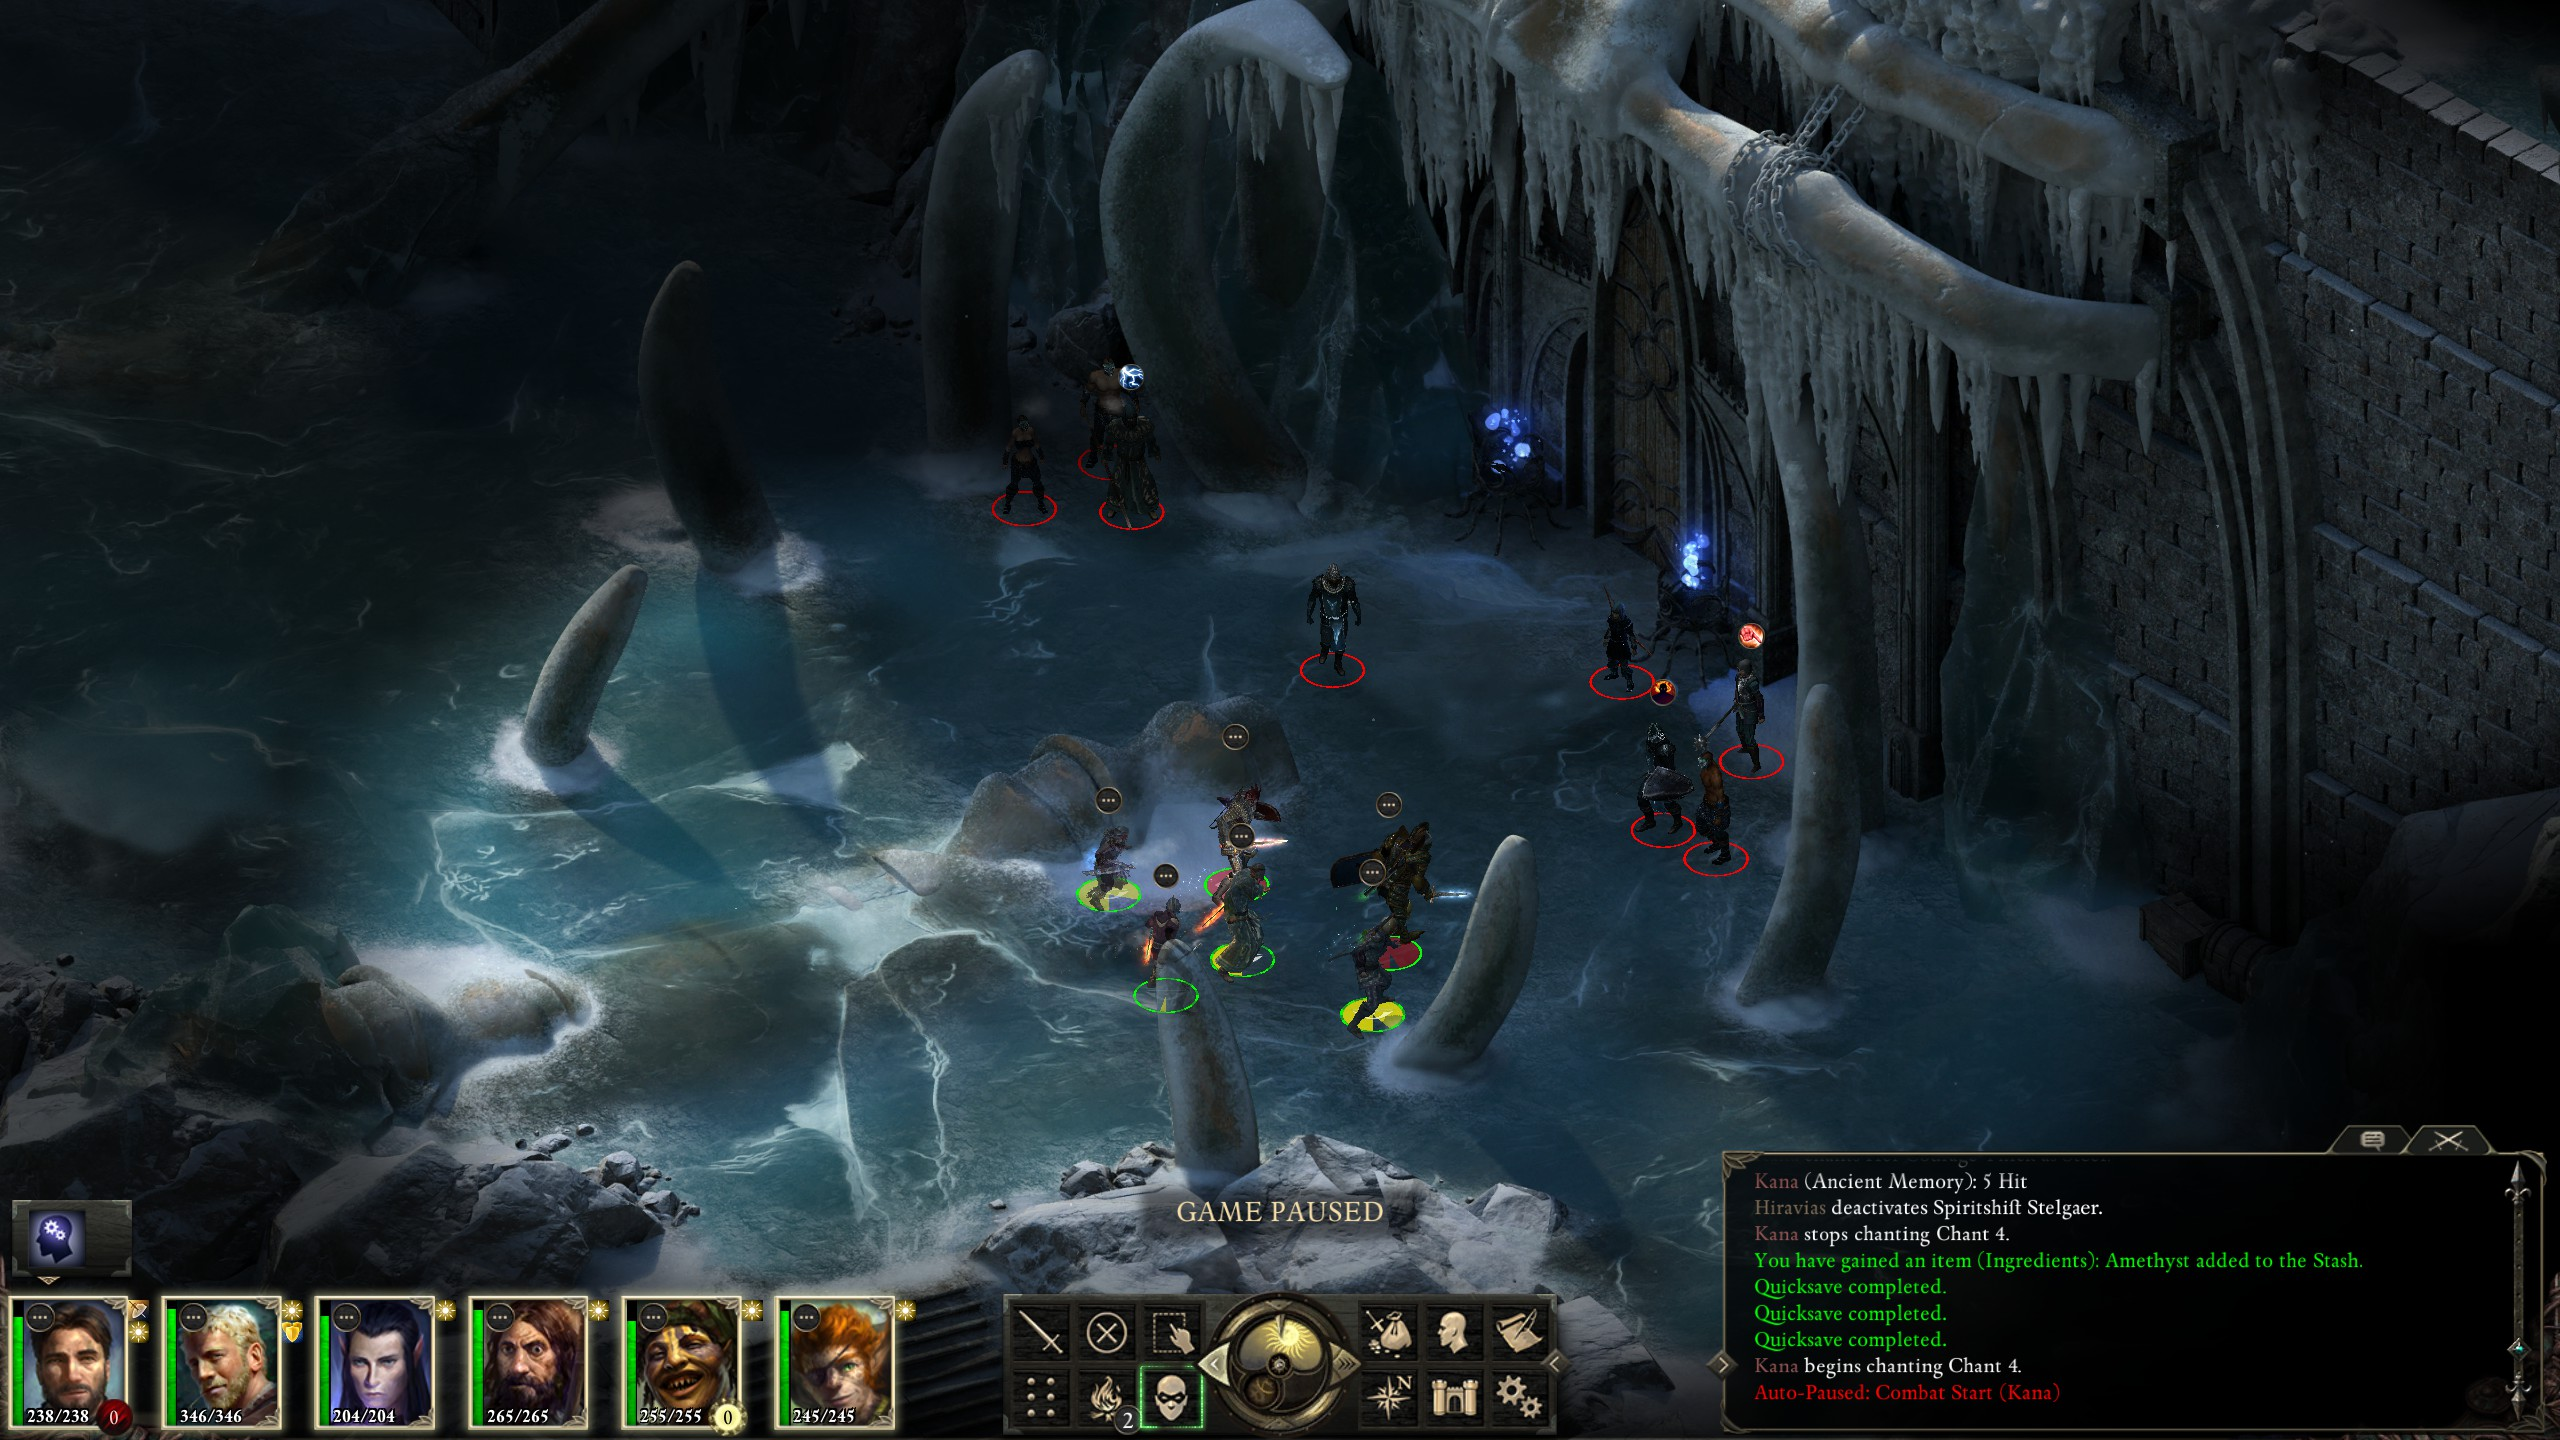
\includegraphics[scale=0.33]{files/blog/2020_01_18_poe_potd_wmpt2/2020_01_18_abbey02.jpg}
\end{figure}

I also ran into a bit of trouble on the west side as I accidentally drew numerous guards into a prolonged fight.

\begin{figure}
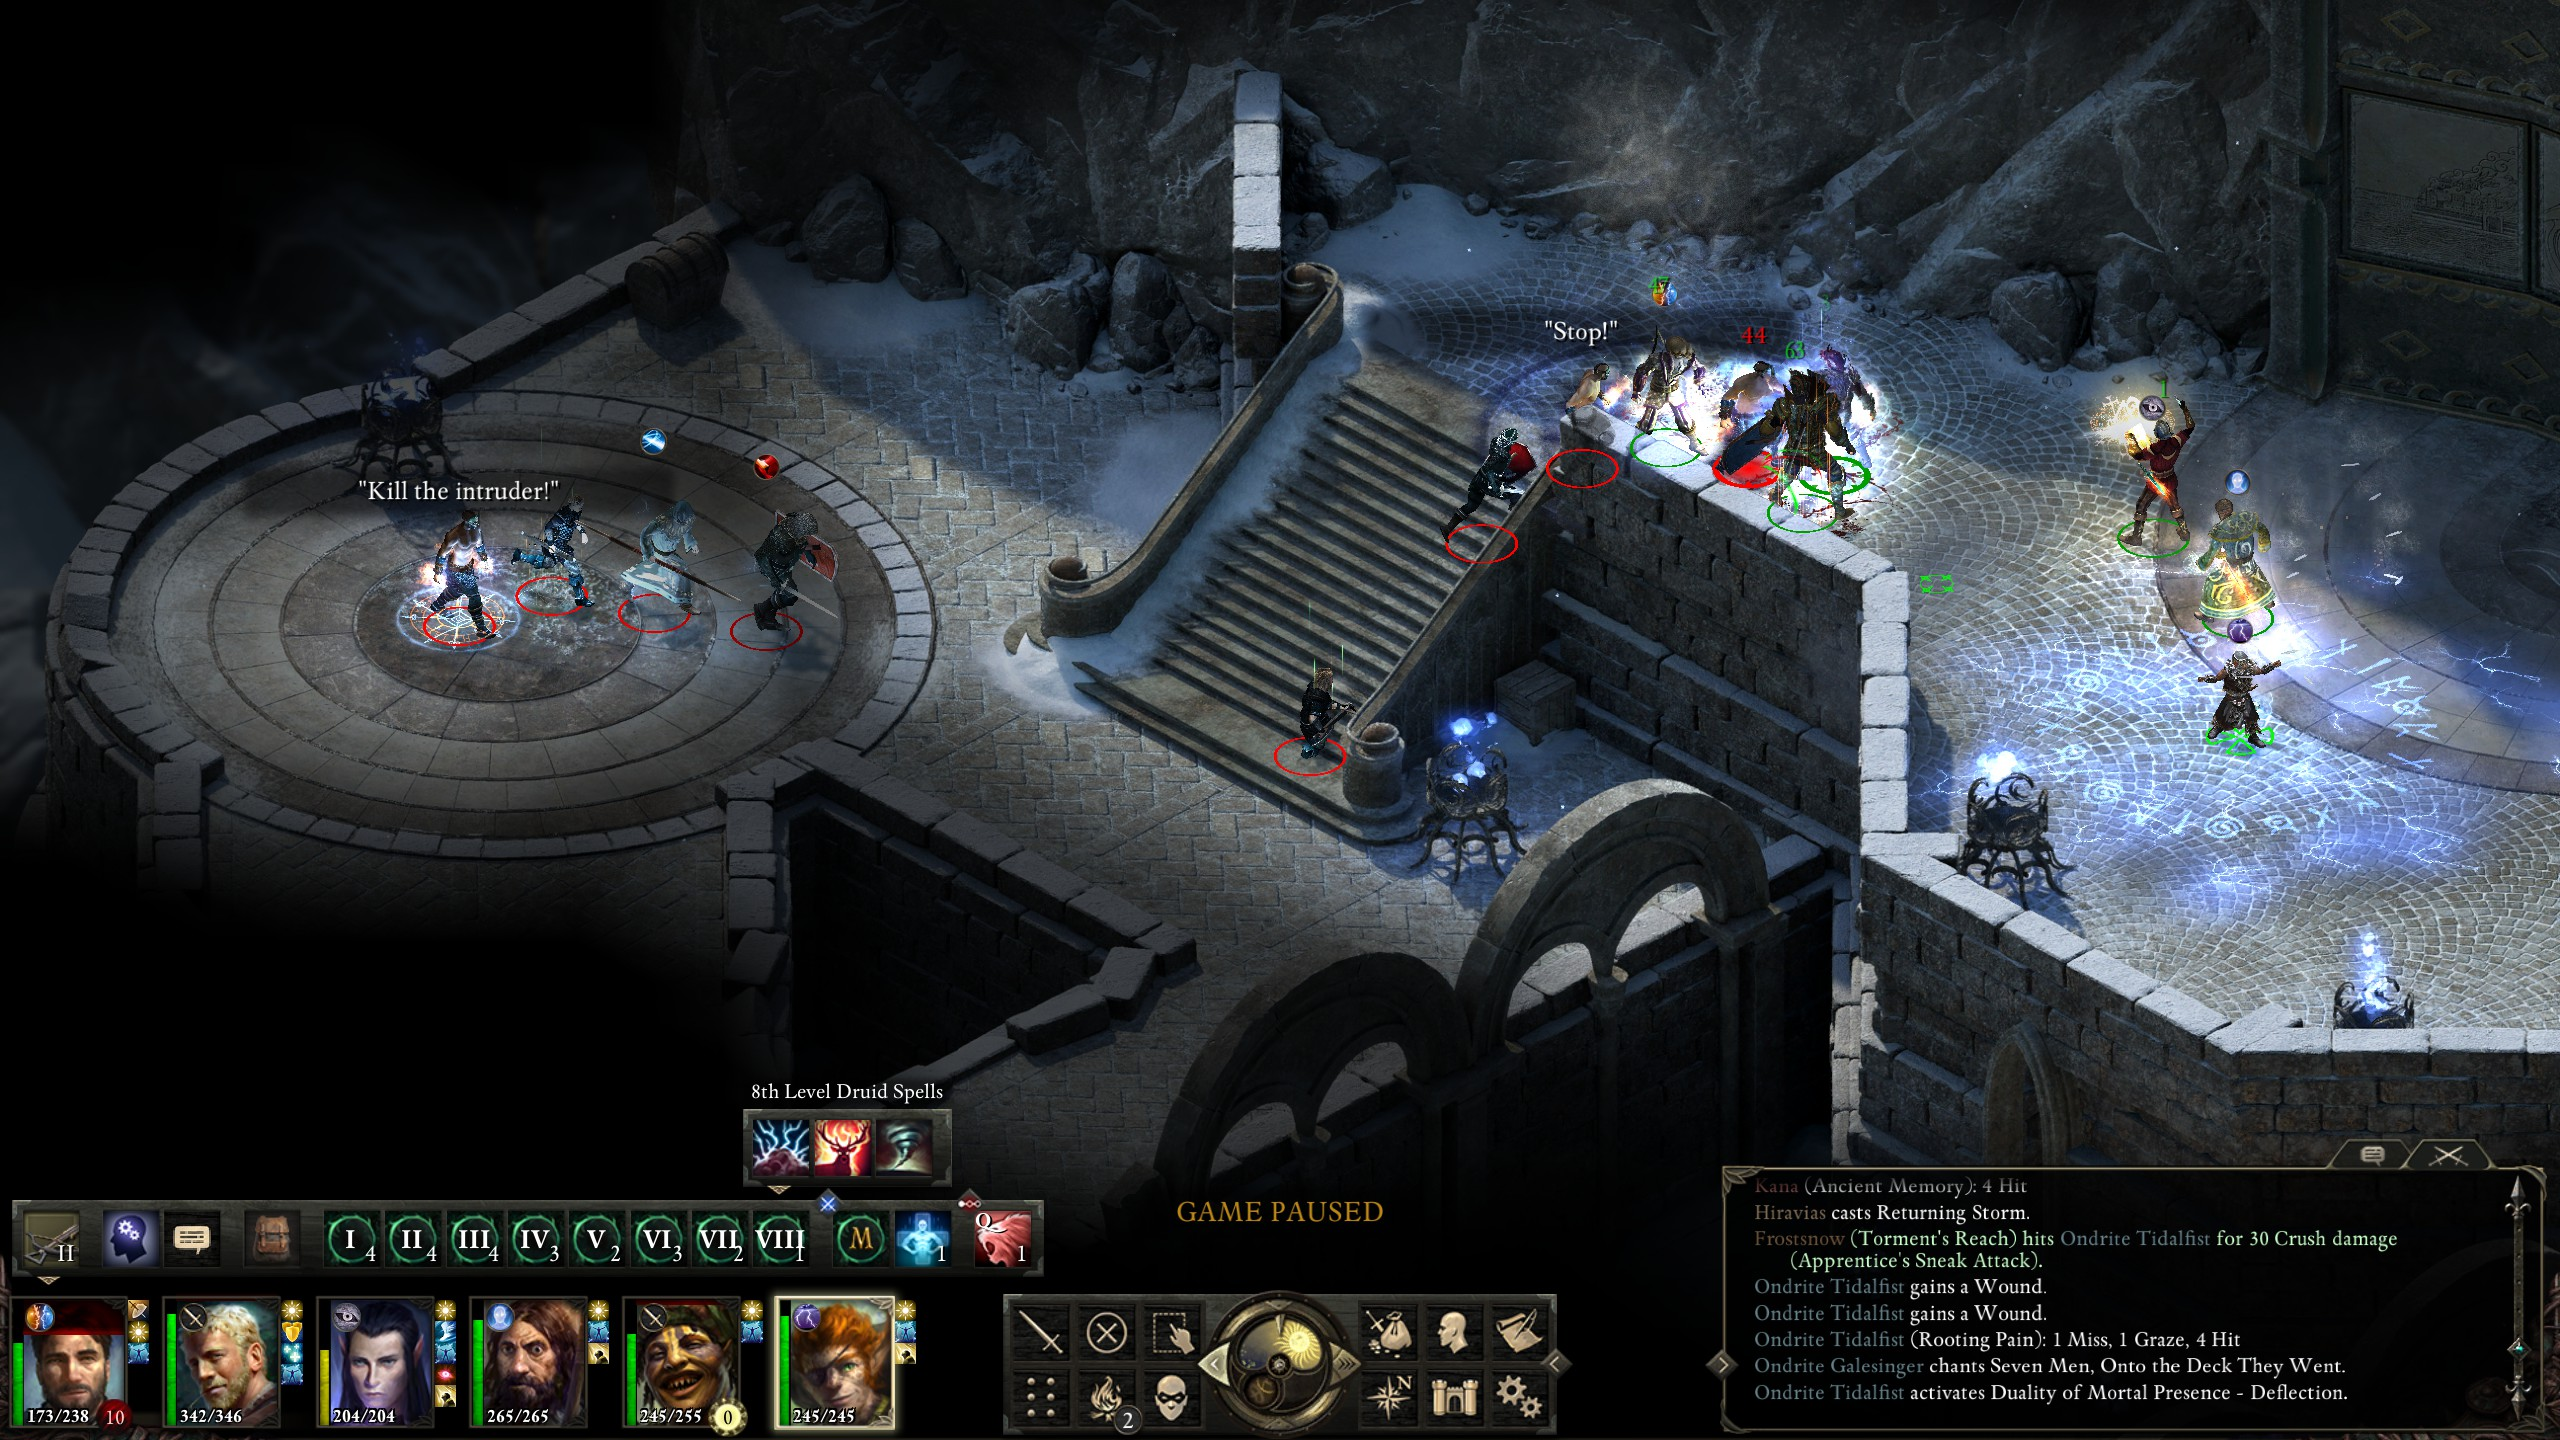
\includegraphics[scale=0.33]{files/blog/2020_01_18_poe_potd_wmpt2/2020_01_18_abbey03.jpg}
\end{figure}

I ended up prevailing, but it was a bit closer than I'd intended.

\begin{figure}
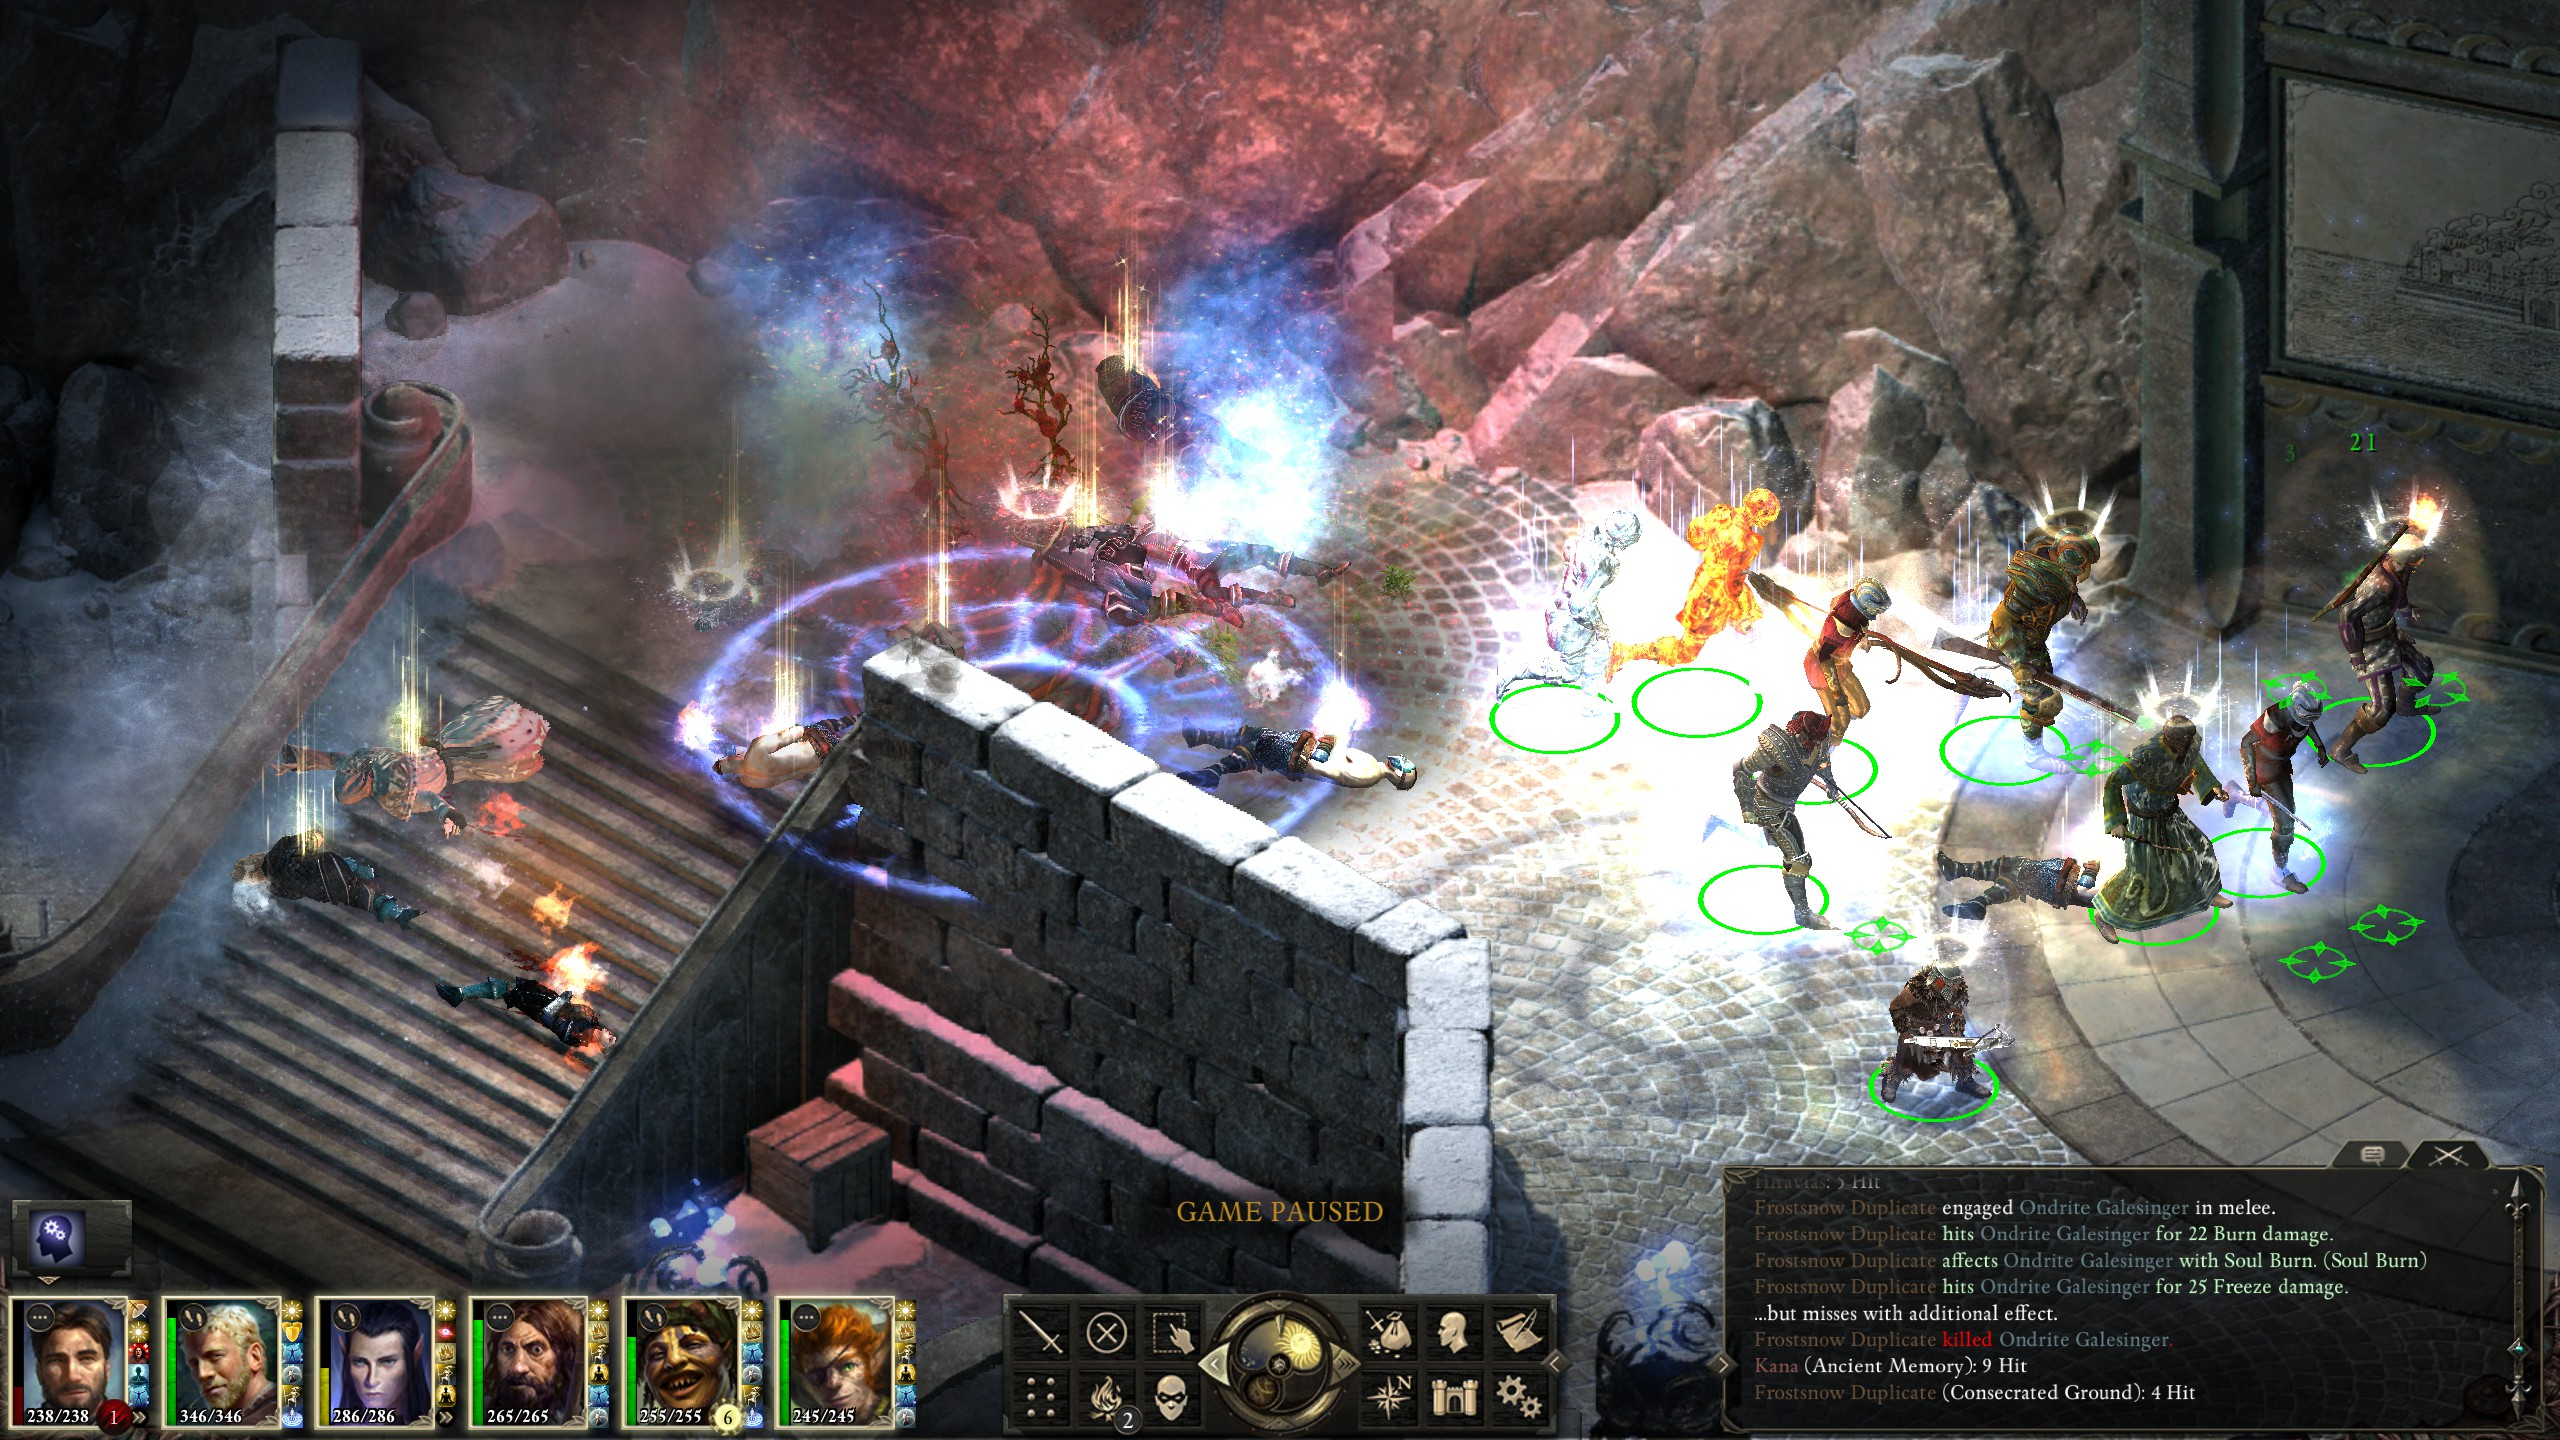
\includegraphics[scale=0.33]{files/blog/2020_01_18_poe_potd_wmpt2/2020_01_18_abbey04.jpg}
\end{figure}

Inside the main entrance to the abbey was this excellent sculpture of a ship being torn apart by a kraken; oh, and a few guards.

\begin{figure}
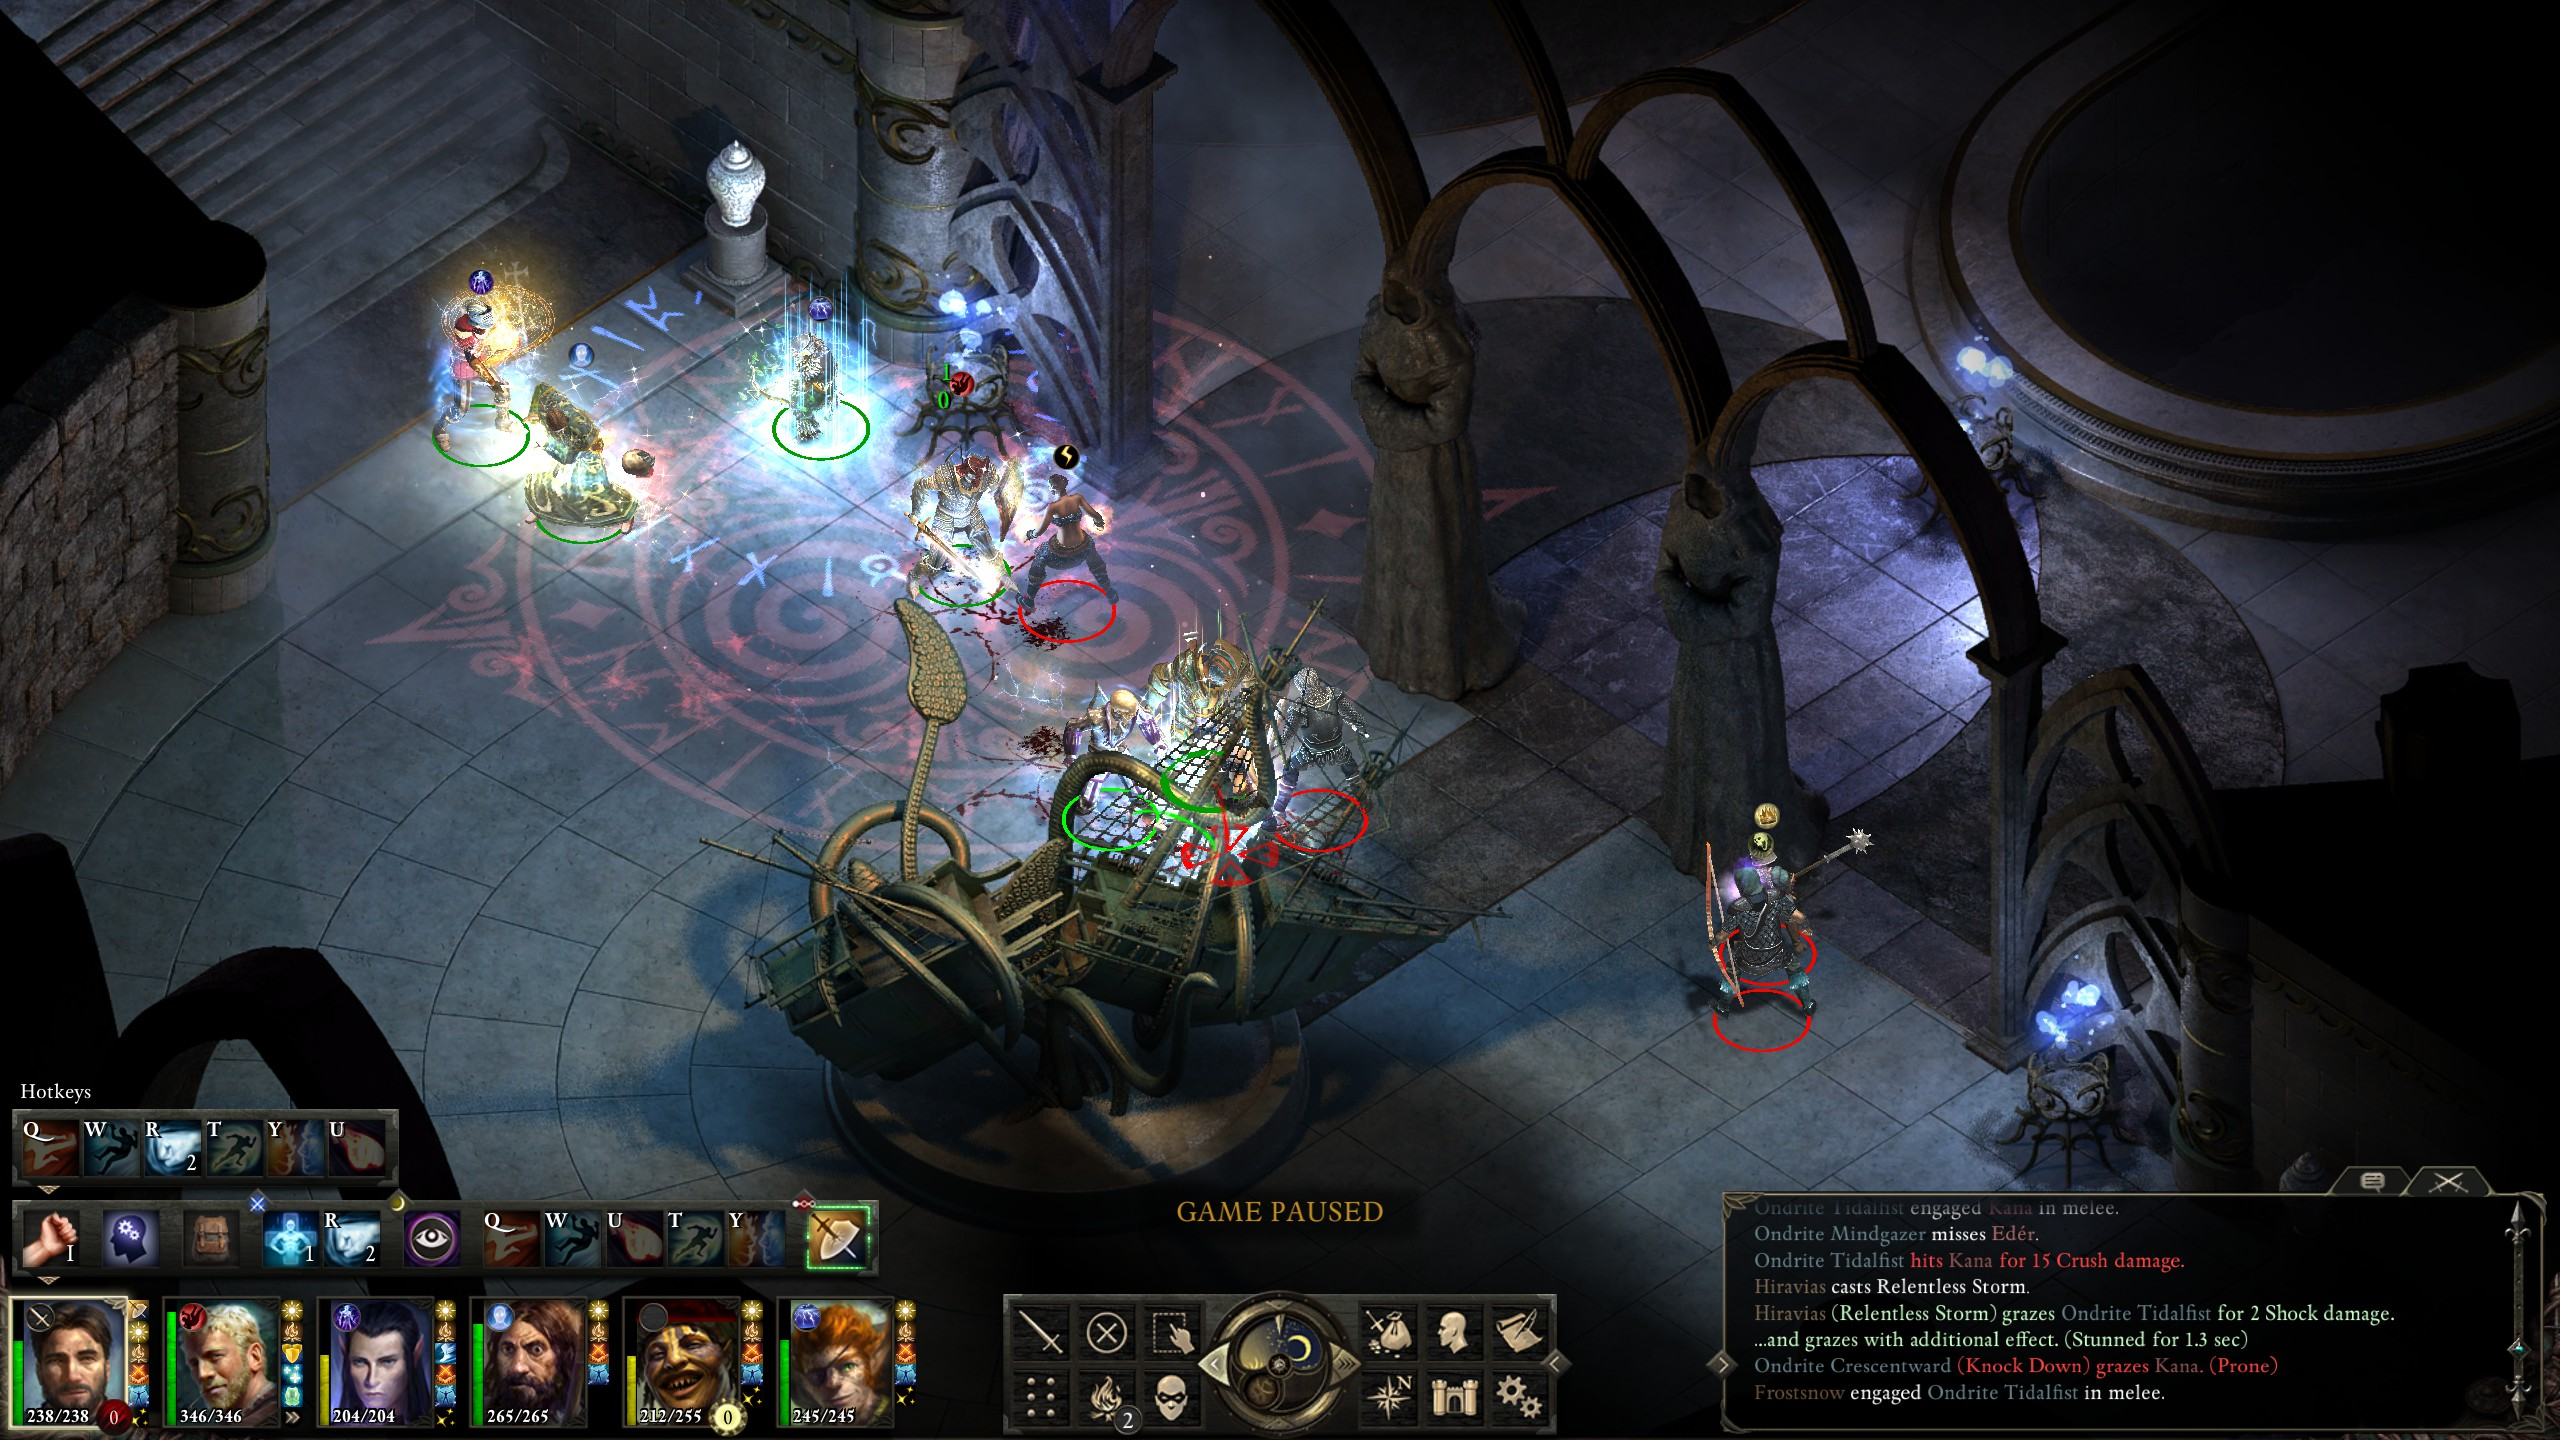
\includegraphics[scale=0.33]{files/blog/2020_01_18_poe_potd_wmpt2/2020_01_18_abbey05.jpg}
\end{figure}

The next room over contained one of the main rooms of the abbey, which was probably the most heavily-guarded of all the rooms.

\begin{figure}
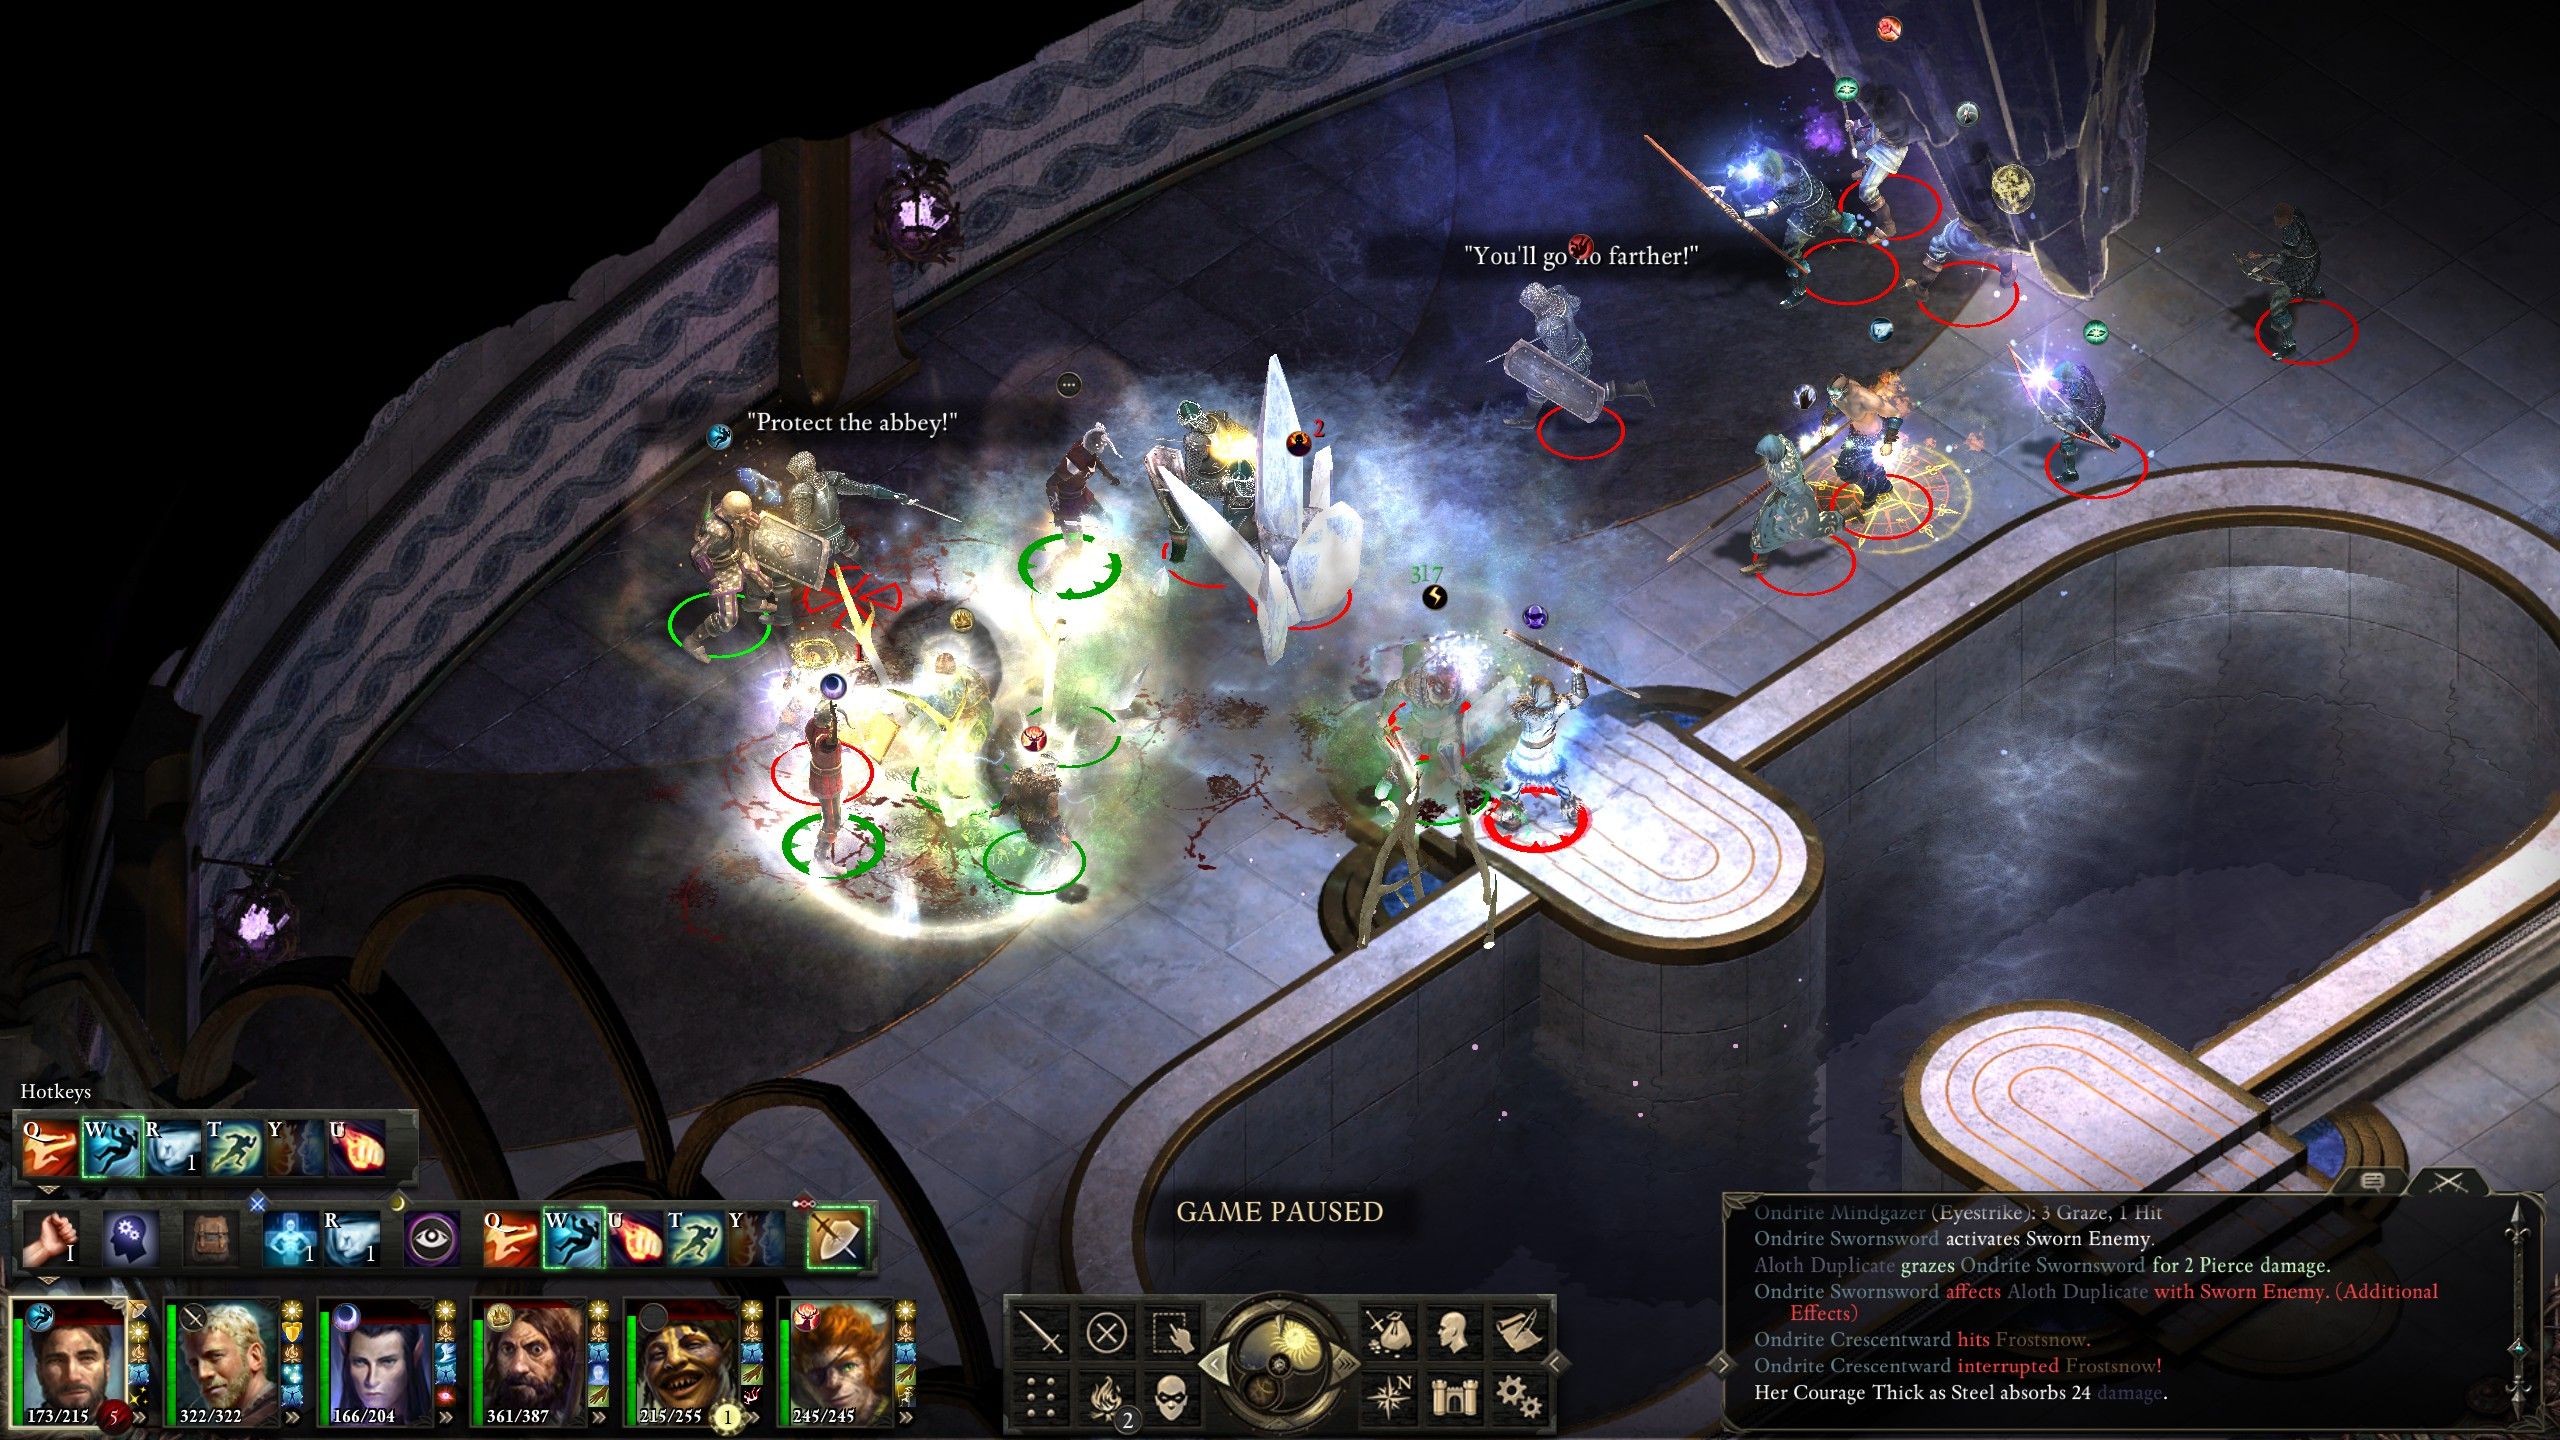
\includegraphics[scale=0.33]{files/blog/2020_01_18_poe_potd_wmpt2/2020_01_18_abbey06.jpg}
\end{figure}

A further room past that was High Abbot Kaoto and his subordinates.  The abbot actually got a good stun and burn-down in on my monk, enough that I had to revive my monk and then have him chain-cast ``Force of Anguish'' on the abbot in order to keep him off my monk.

\begin{figure}
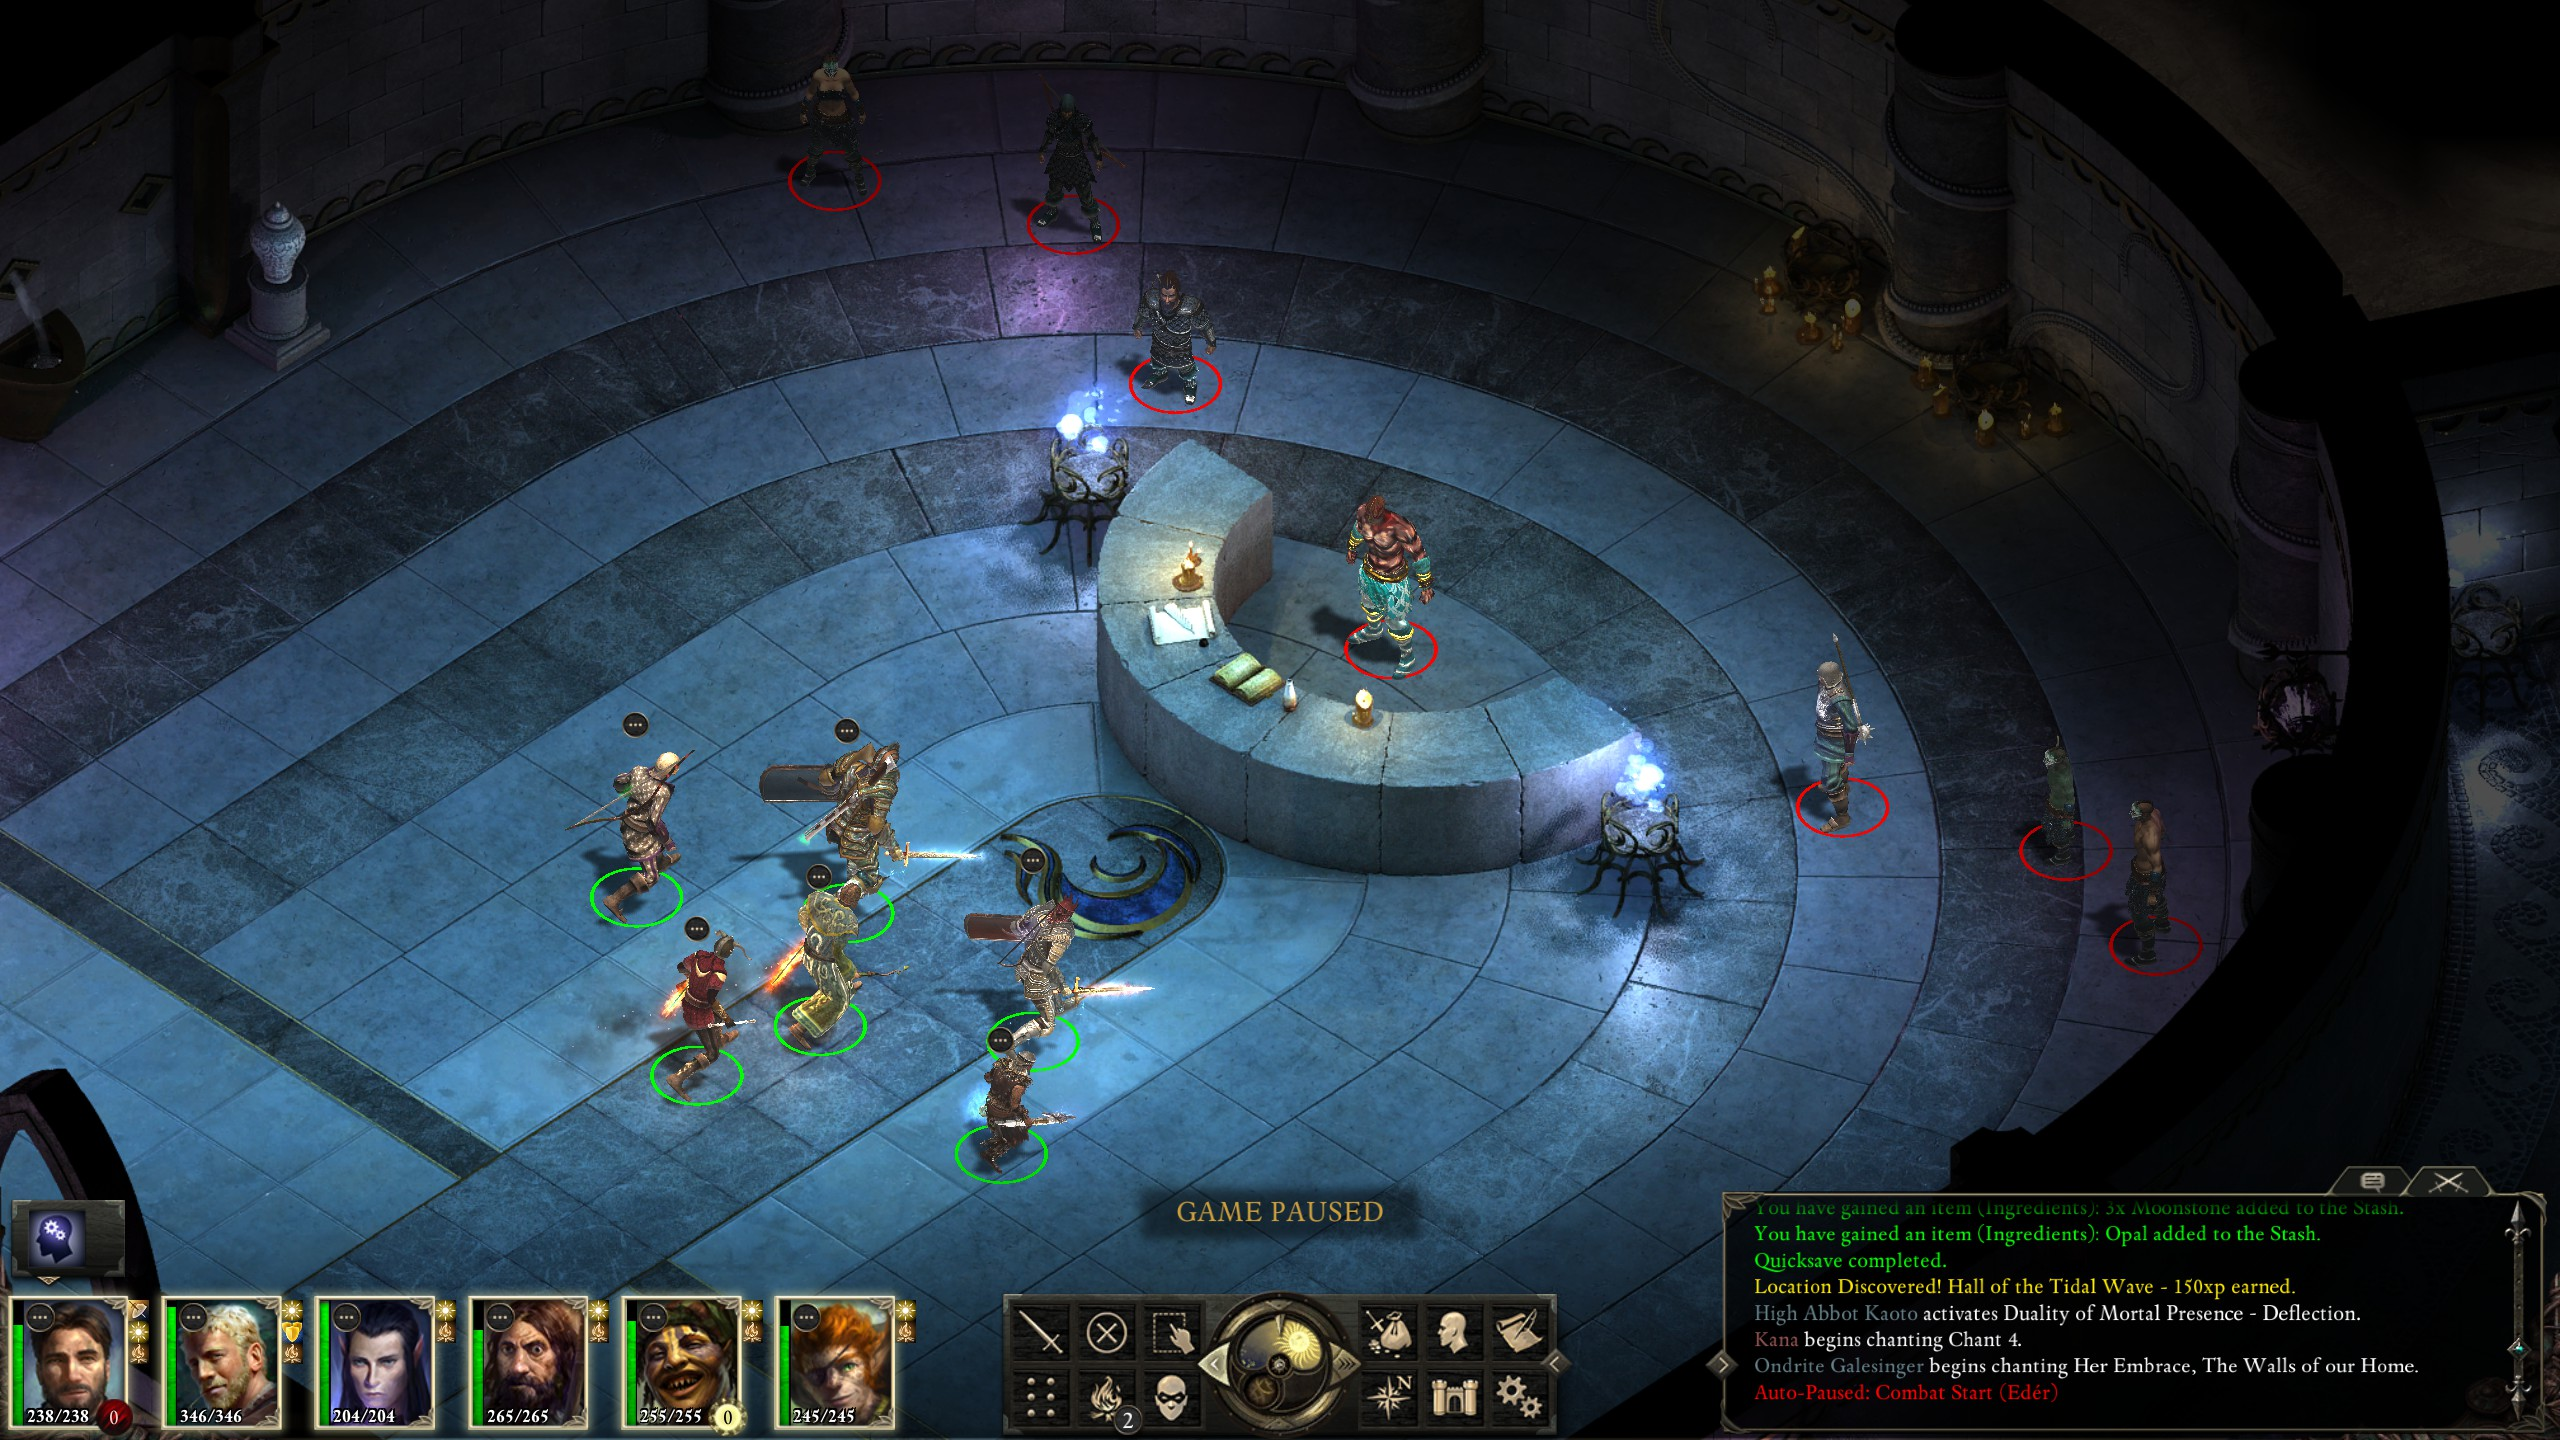
\includegraphics[scale=0.33]{files/blog/2020_01_18_poe_potd_wmpt2/2020_01_18_abbey07.jpg}
\end{figure}

Below the first floor were the quarters where the low tide were kept.

\begin{figure}
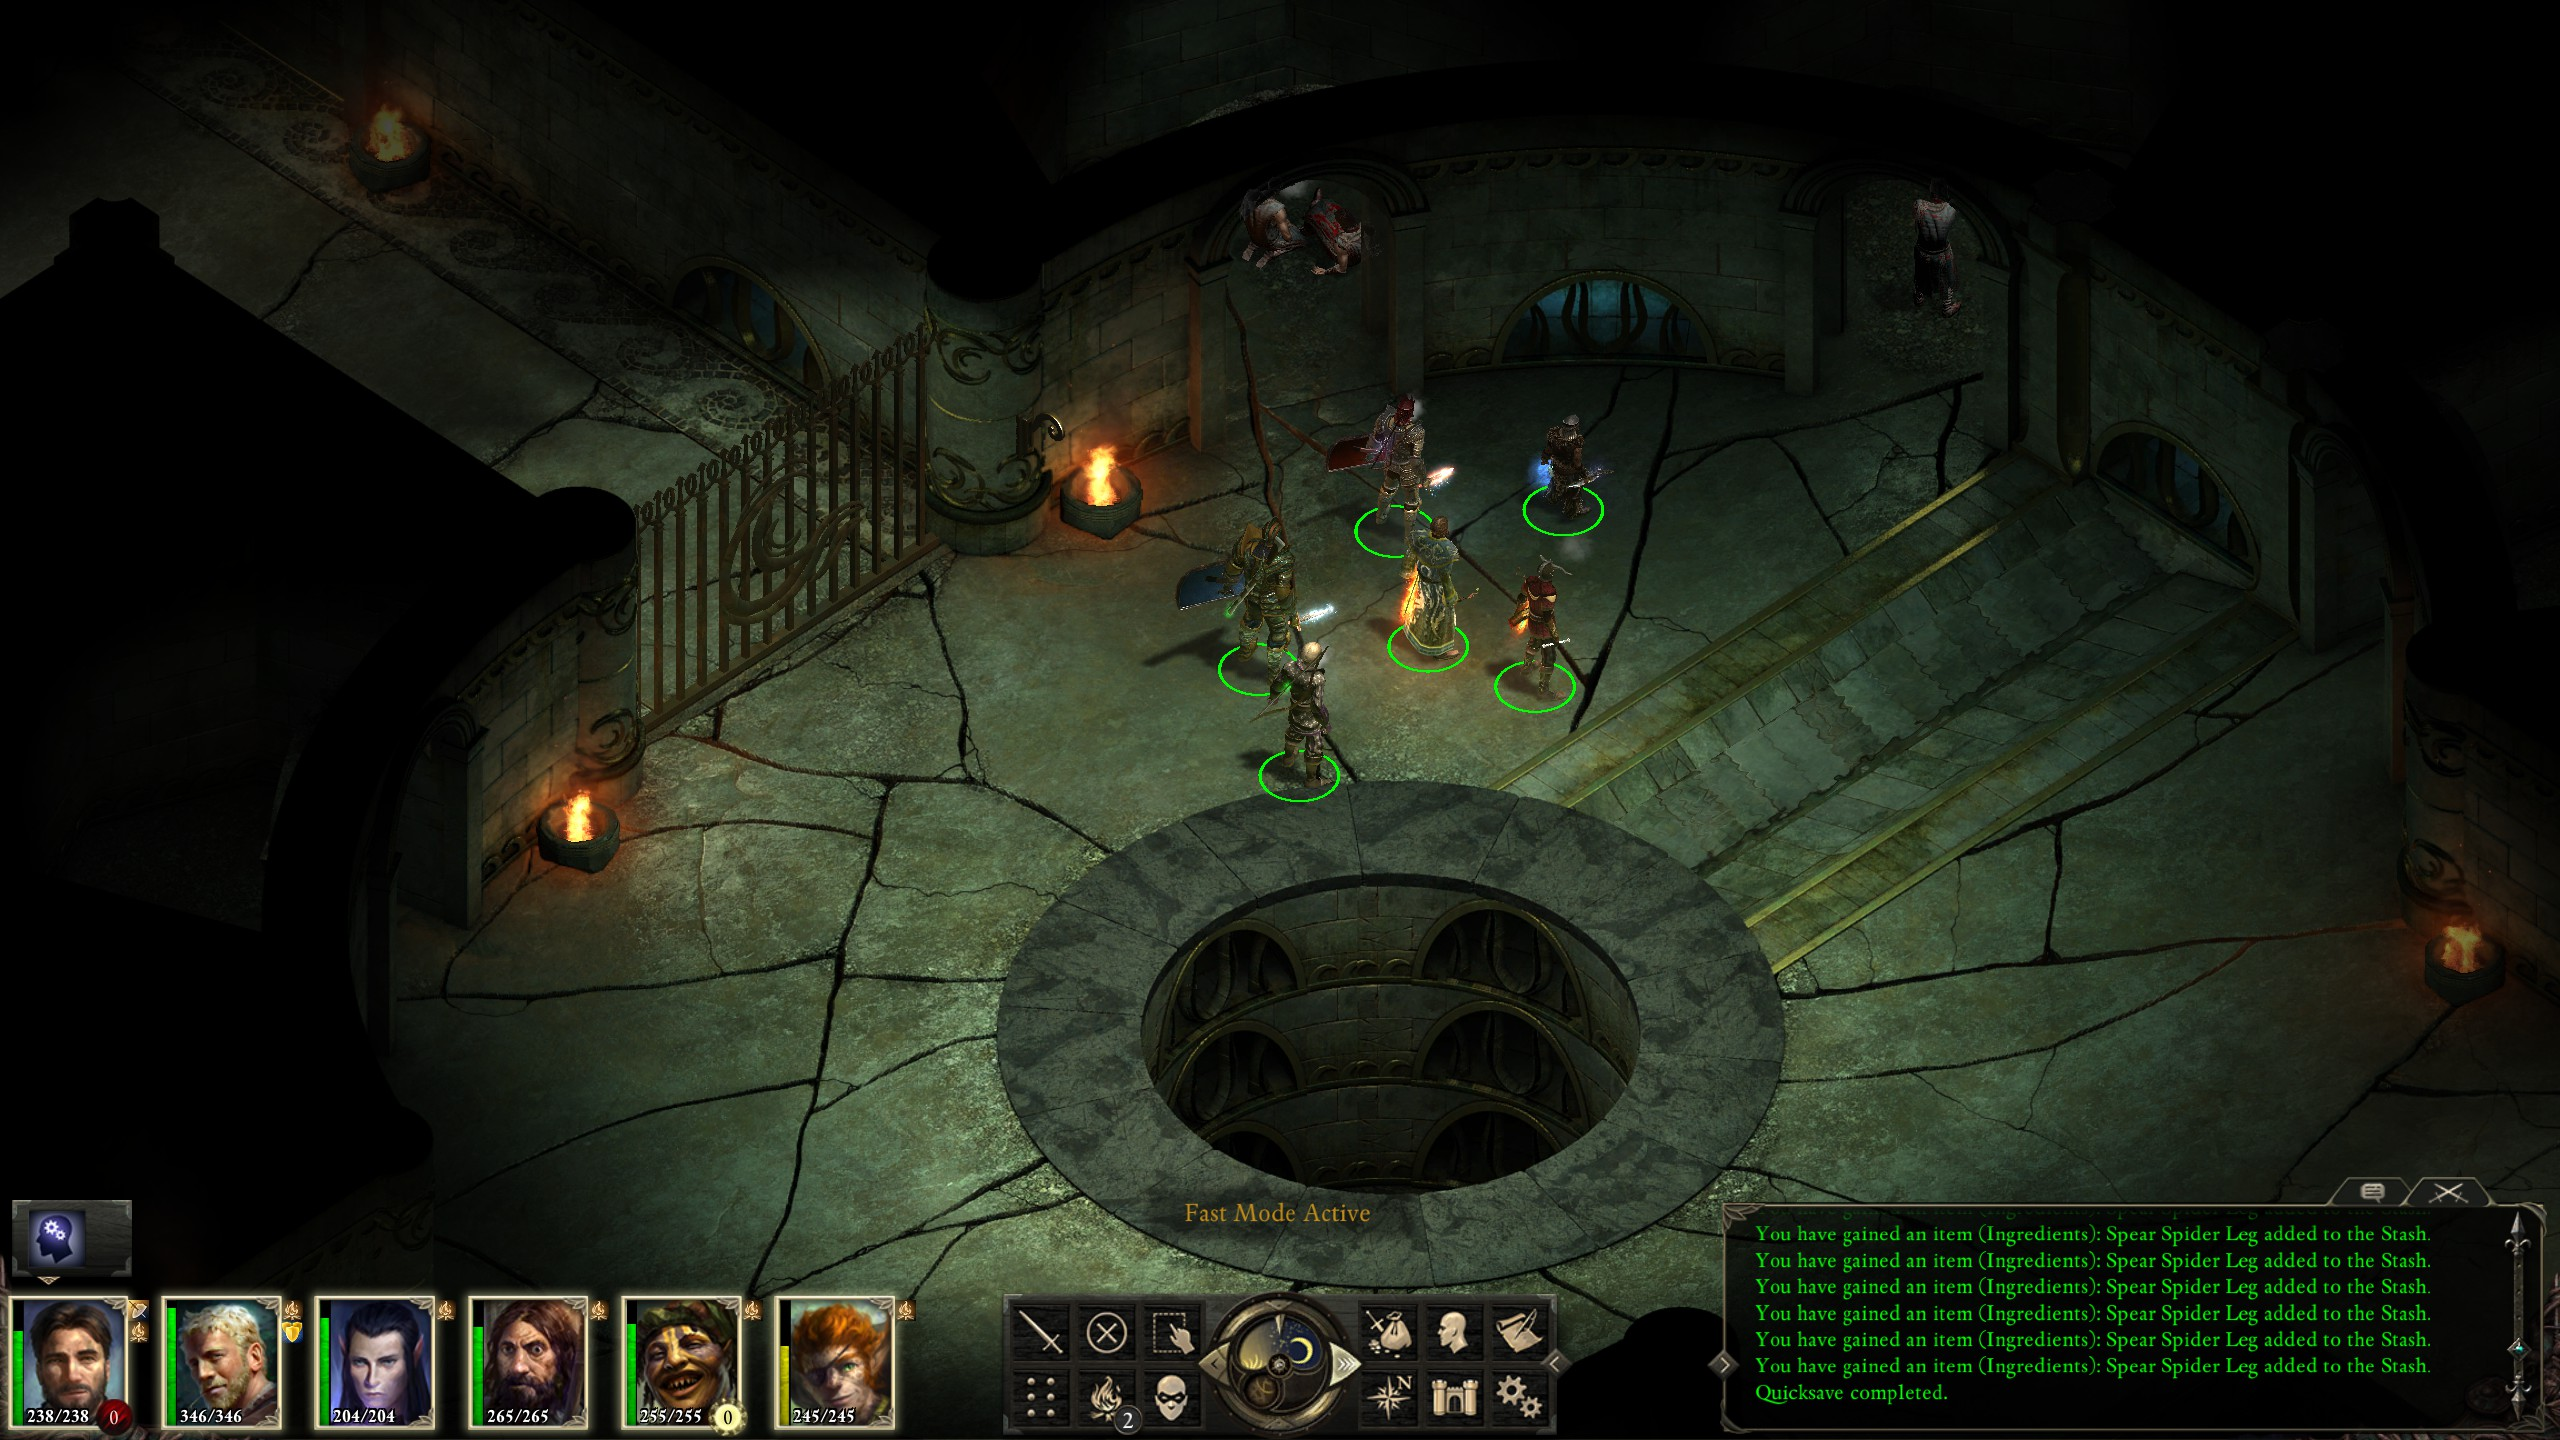
\includegraphics[scale=0.33]{files/blog/2020_01_18_poe_potd_wmpt2/2020_01_18_abbey08.jpg}
\end{figure}

After working through their quarters and solving a puzzle, I traversed across the magical water bridge towards Ondra's Wirness.

\begin{figure}
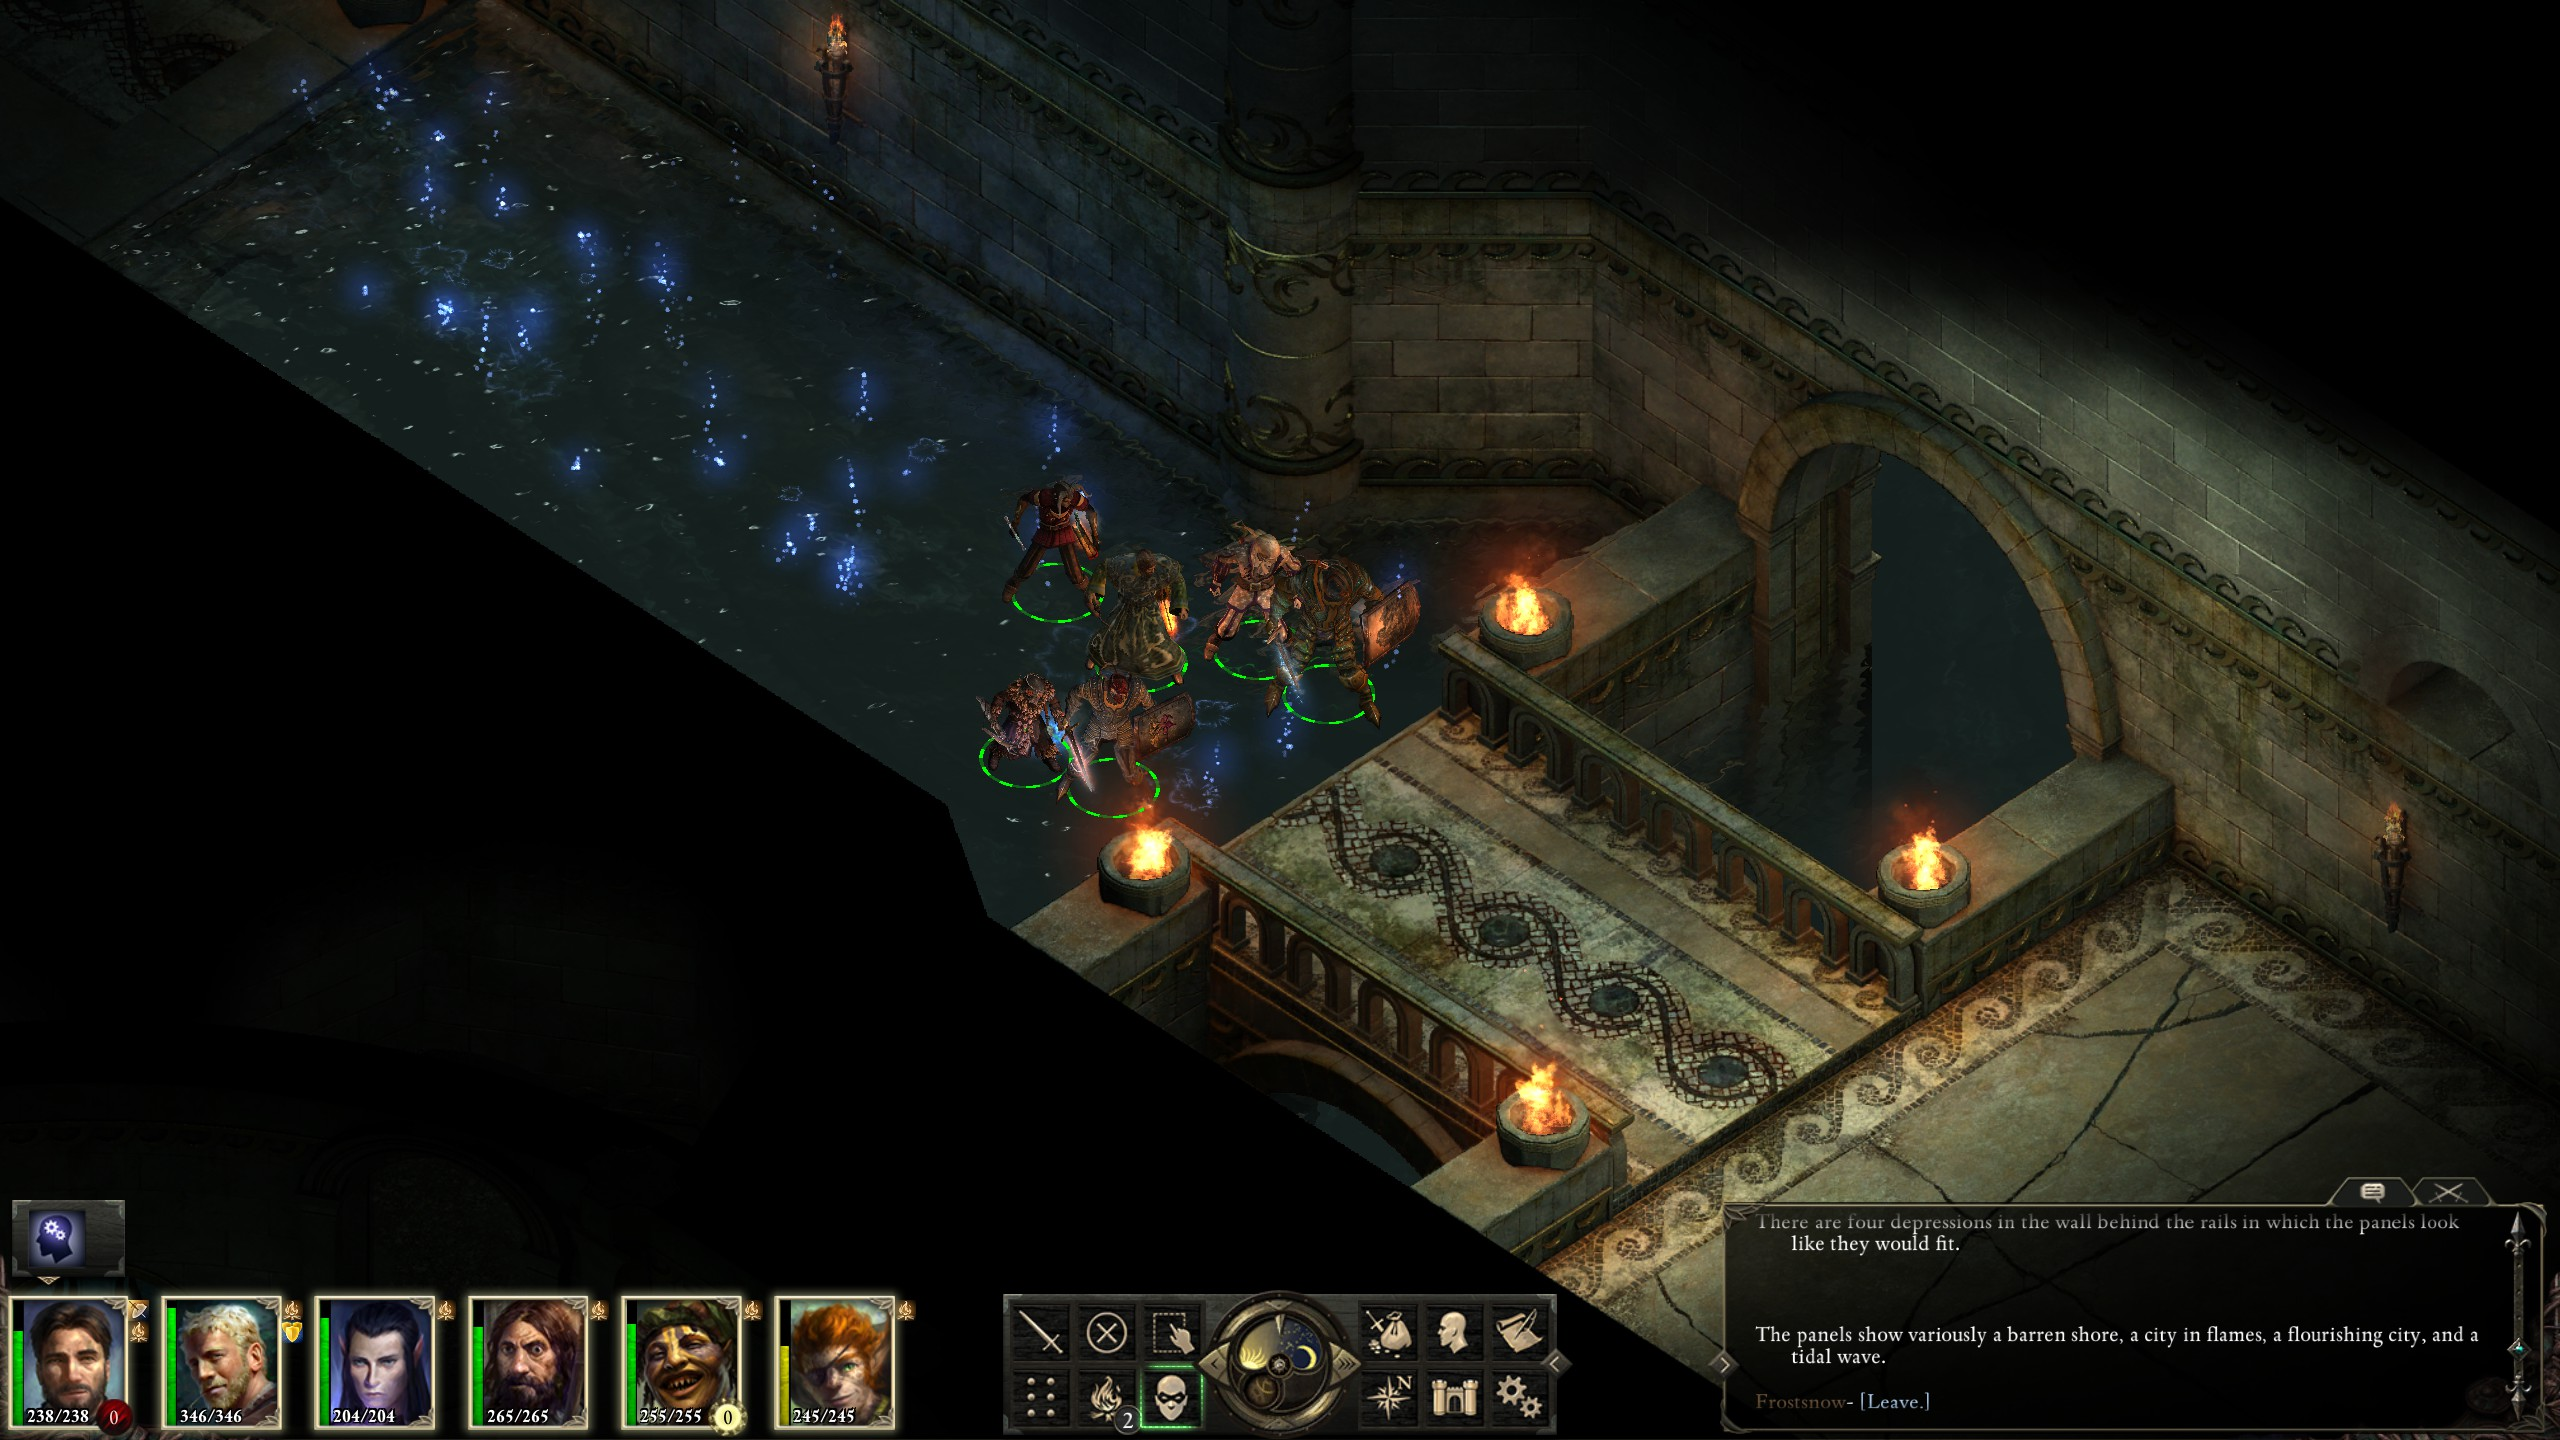
\includegraphics[scale=0.33]{files/blog/2020_01_18_poe_potd_wmpt2/2020_01_18_abbey09.jpg}
\end{figure}

At the Chamber of Tears I decided to release the low tide rather than drowning them as per the past abbot's request.  The high tide wasn't able to do much about it given that I'd just finished massacring them.

\begin{figure}
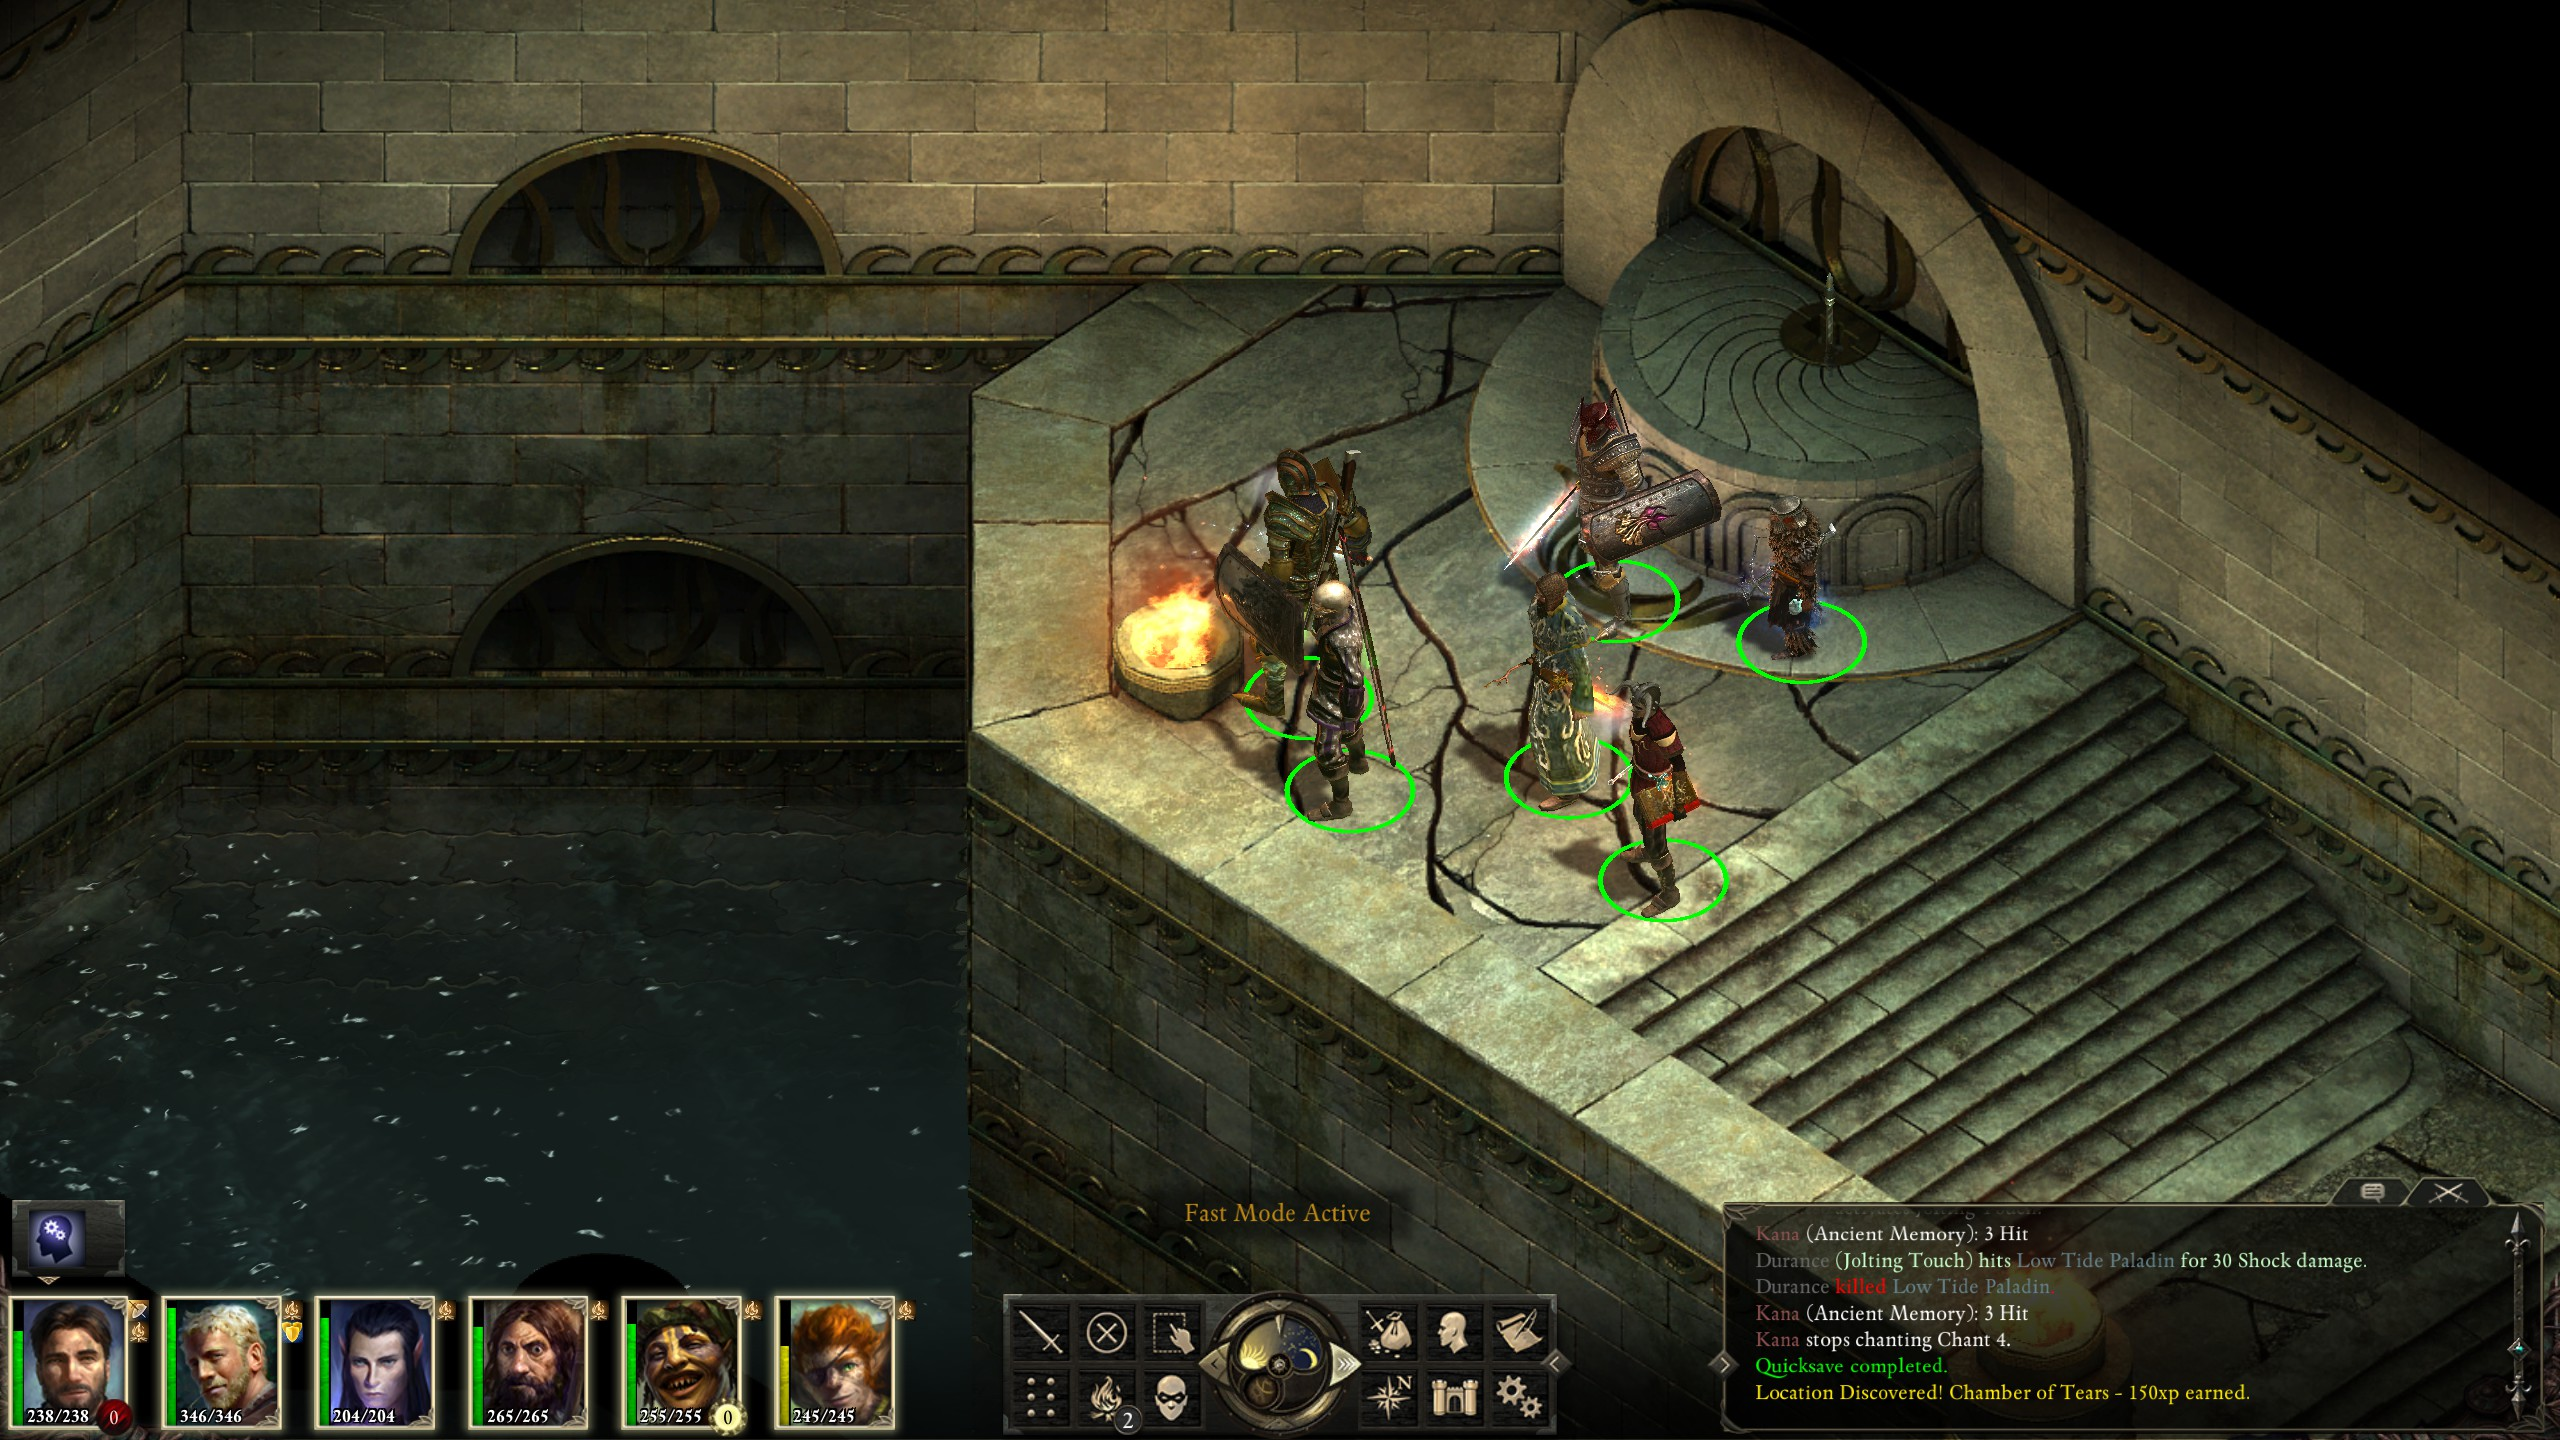
\includegraphics[scale=0.33]{files/blog/2020_01_18_poe_potd_wmpt2/2020_01_18_abbey10.jpg}
\end{figure}

On the way out I noticed what appeared to be another exquisite kraken statue.  The foreshadowing is strong with this one.

\begin{figure}
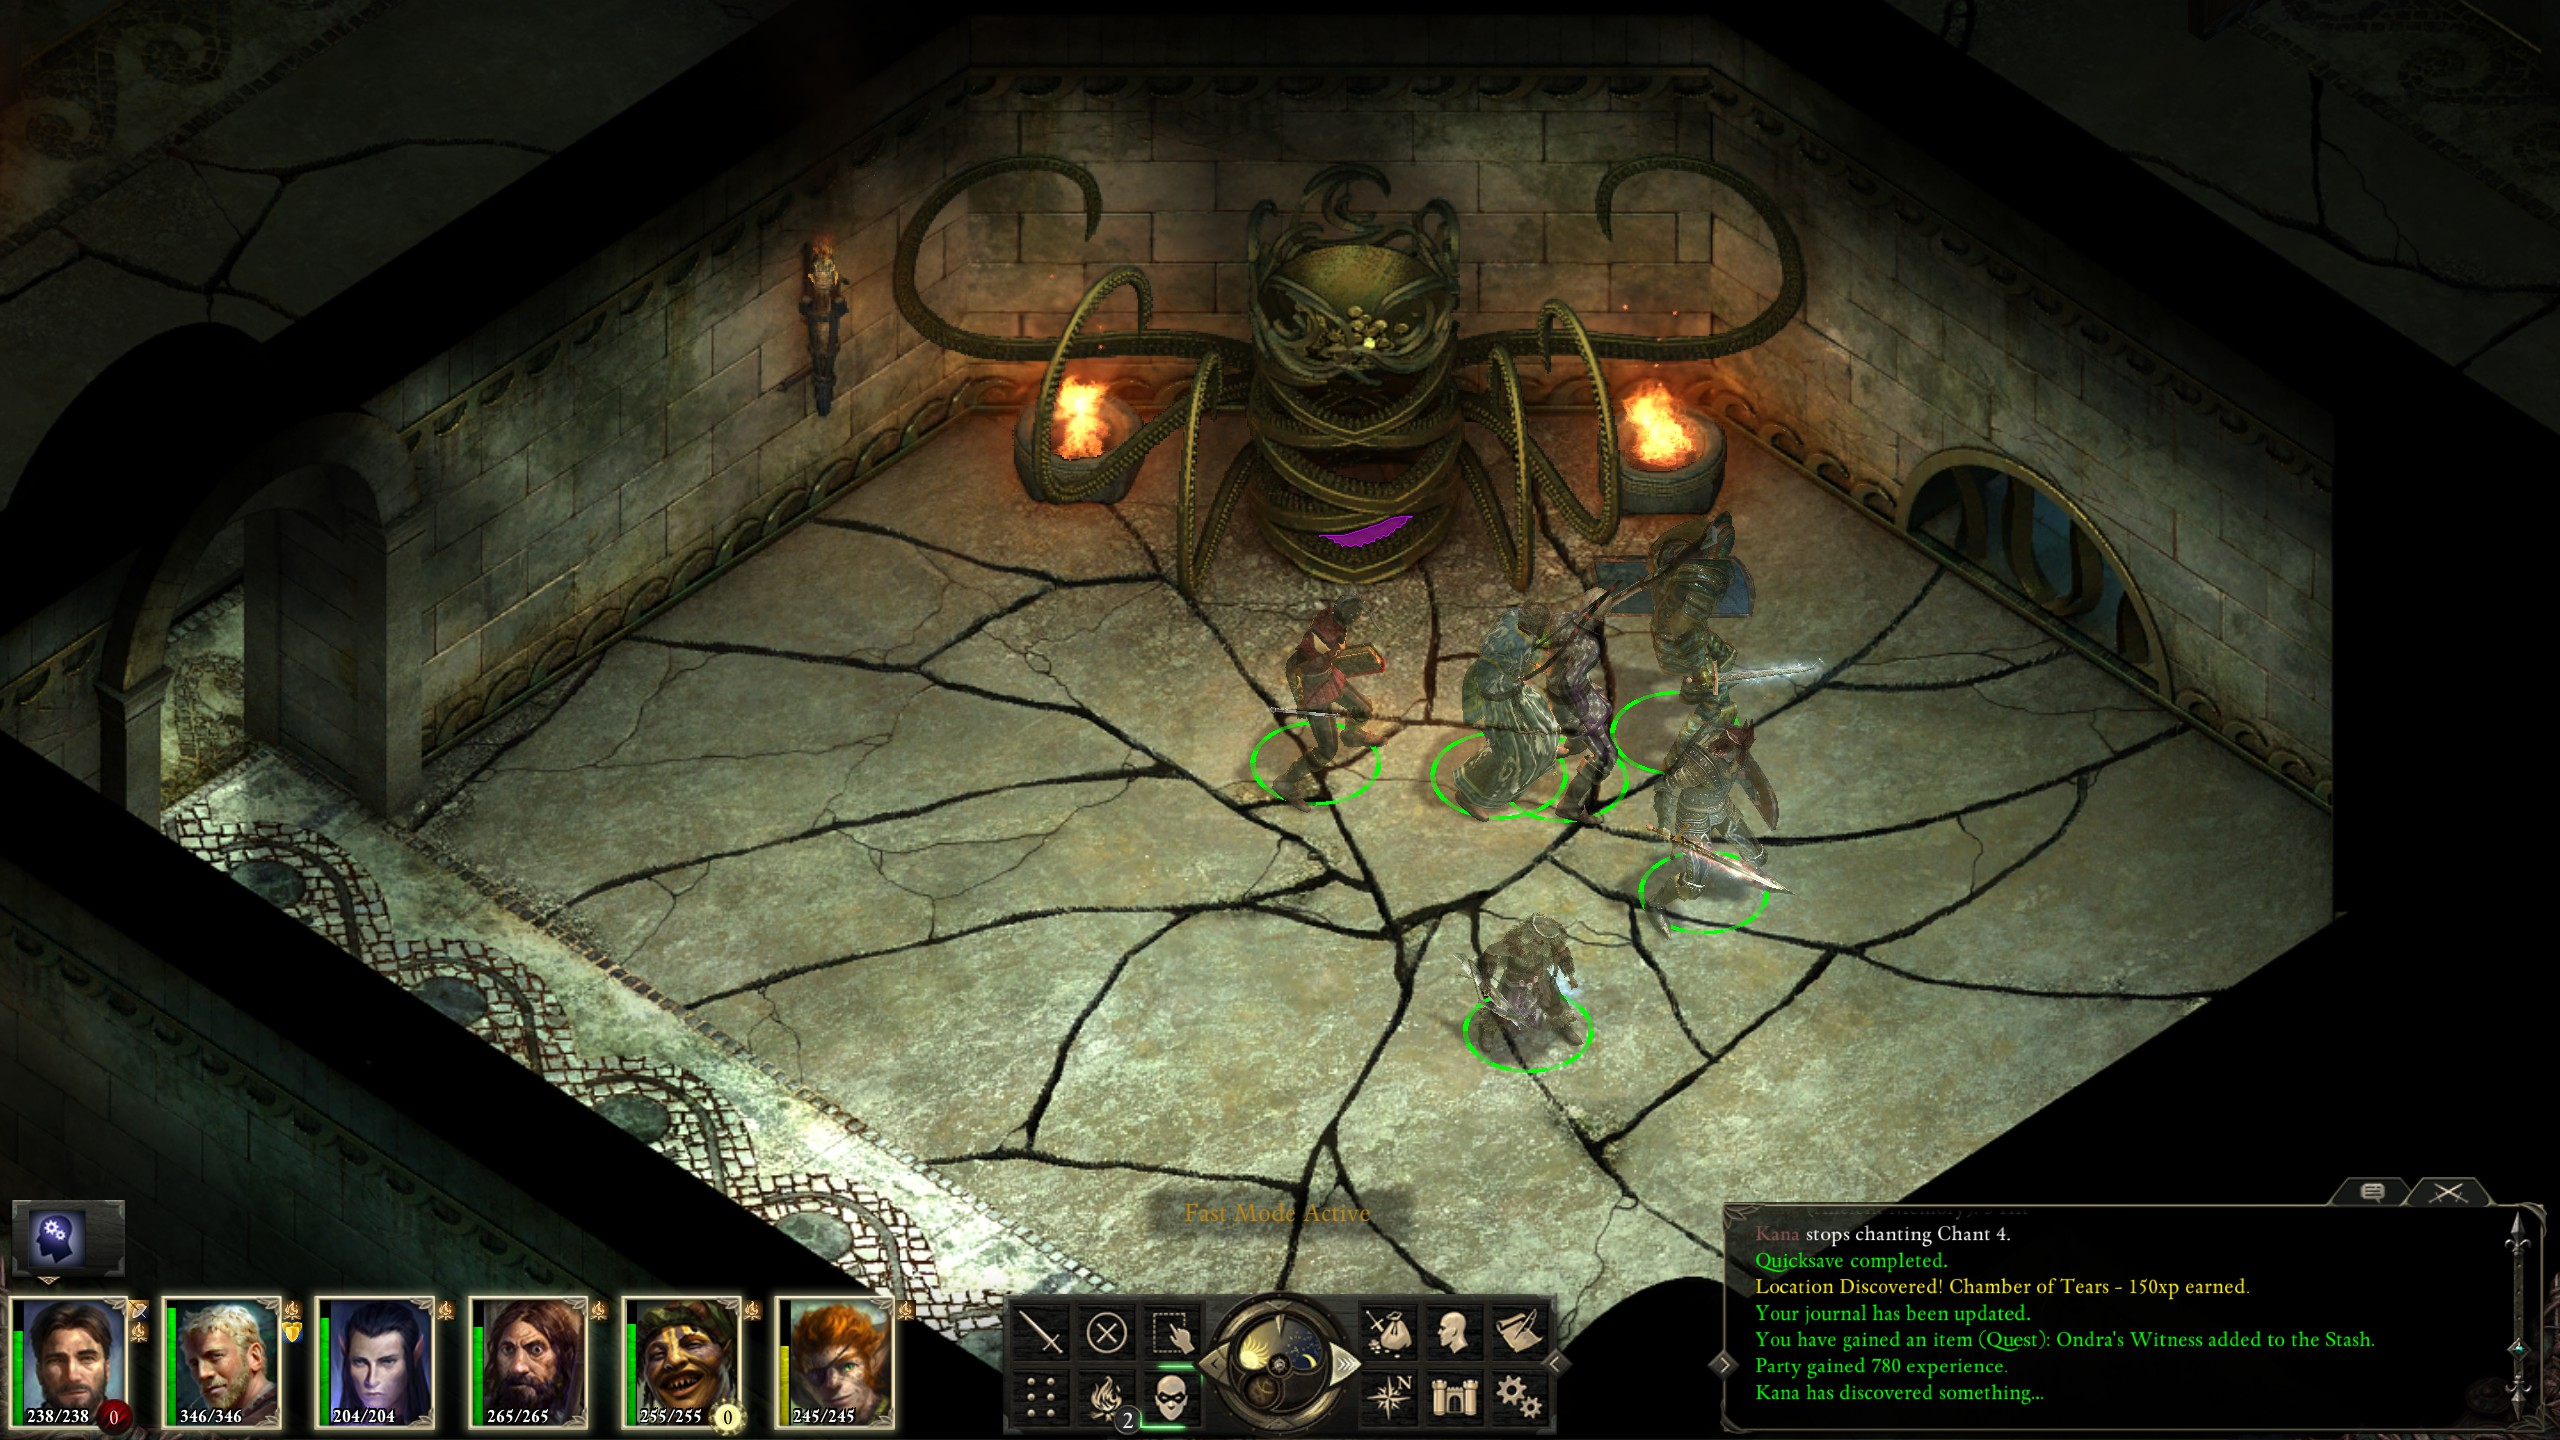
\includegraphics[scale=0.33]{files/blog/2020_01_18_poe_potd_wmpt2/2020_01_18_abbey11.jpg}
\end{figure}

Ondra's Witness in hand, I proceeded to the top of the temple where Abydon's fractured skull lay, until now, safely hidden.

\begin{figure}
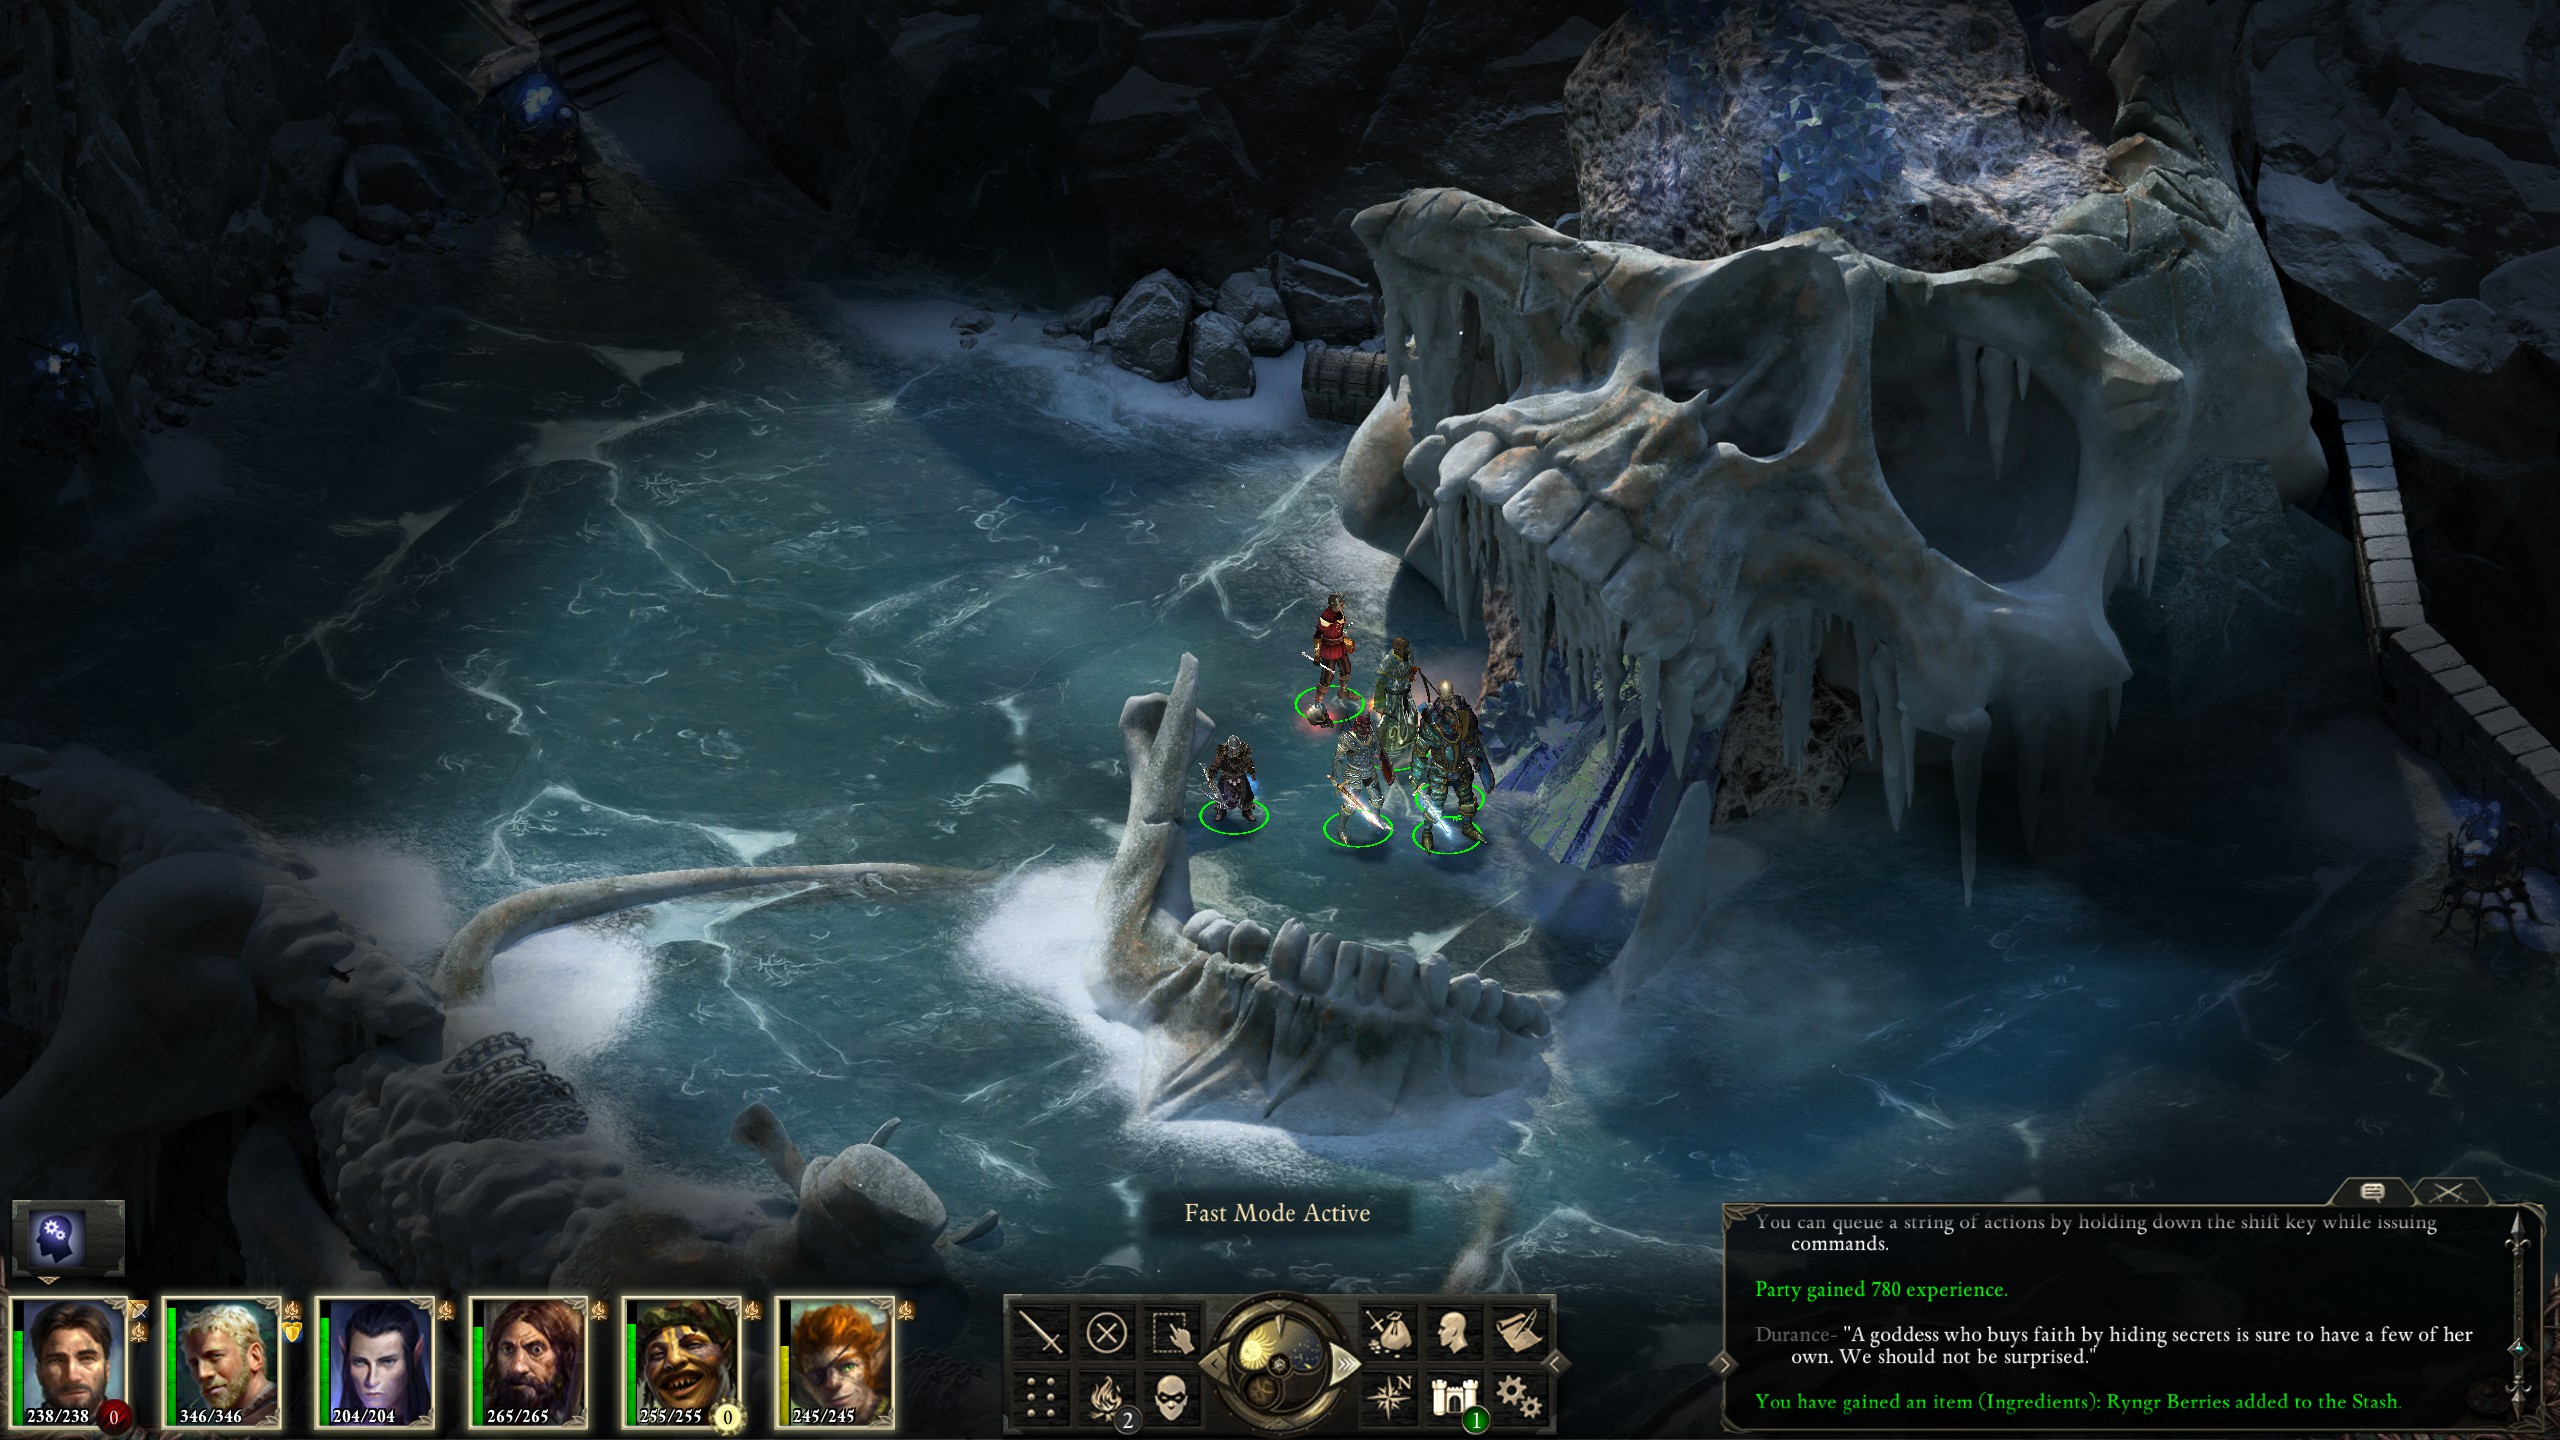
\includegraphics[scale=0.33]{files/blog/2020_01_18_poe_potd_wmpt2/2020_01_18_abbey12.jpg}
\end{figure}

Too bad about Ondra's little secret.  I then took the fragment of Abydon's Hammer, reforged it, and headed over to Crayon's Scar in order to stop the eyeless.

\subsection{Cayron's Scar}
The final area of the main storyline was set in and around a largely-frozen lake with large numbers of eyeless and a few stray tentacles.  The main danger with the eyeless was their ``Ray of Fire'' equivalent, which rapidly drained the endurance of even my tank without Hiravias' ``Weather the Storm'' buff.  Other than that, the eyeless could be disabled easily enough with prone afflictions and focus-firing.

\begin{figure}
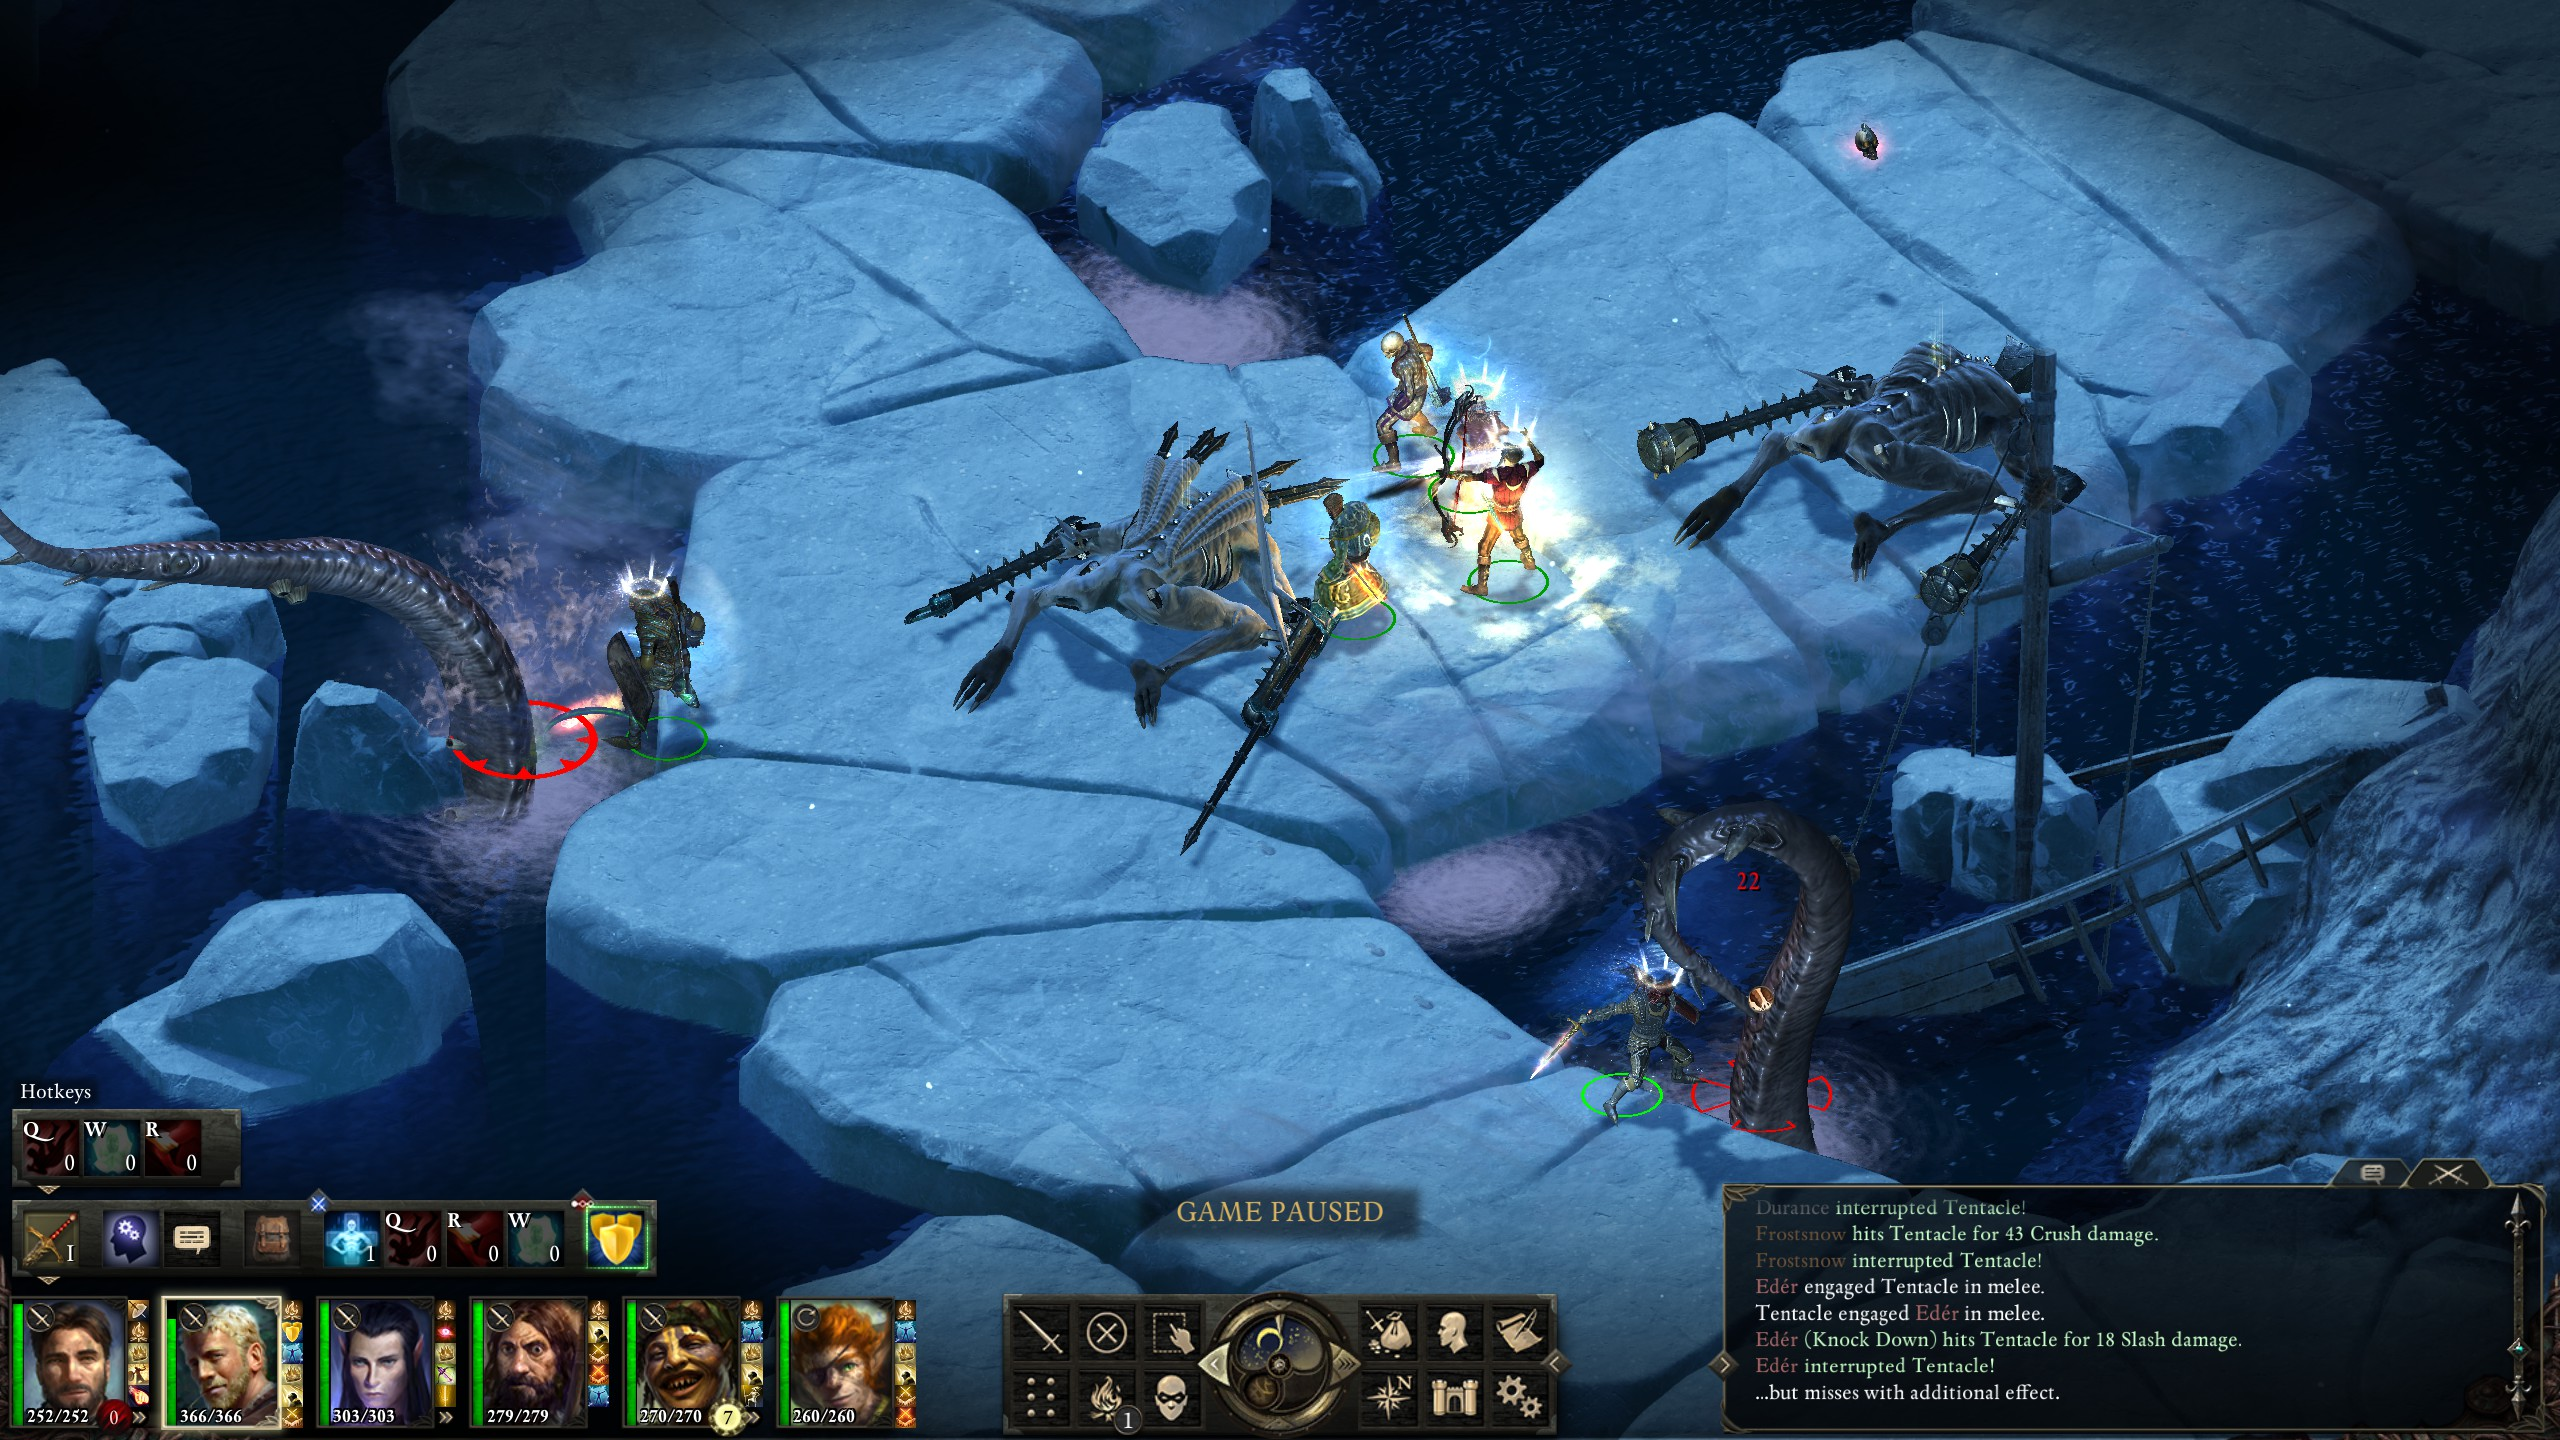
\includegraphics[scale=0.33]{files/blog/2020_01_18_poe_potd_wmpt2/2020_01_18_cayron1.jpg}
\end{figure}

Within the moon floating in the middle of the lake I eventually found, surprise, a kraken!

\begin{figure}
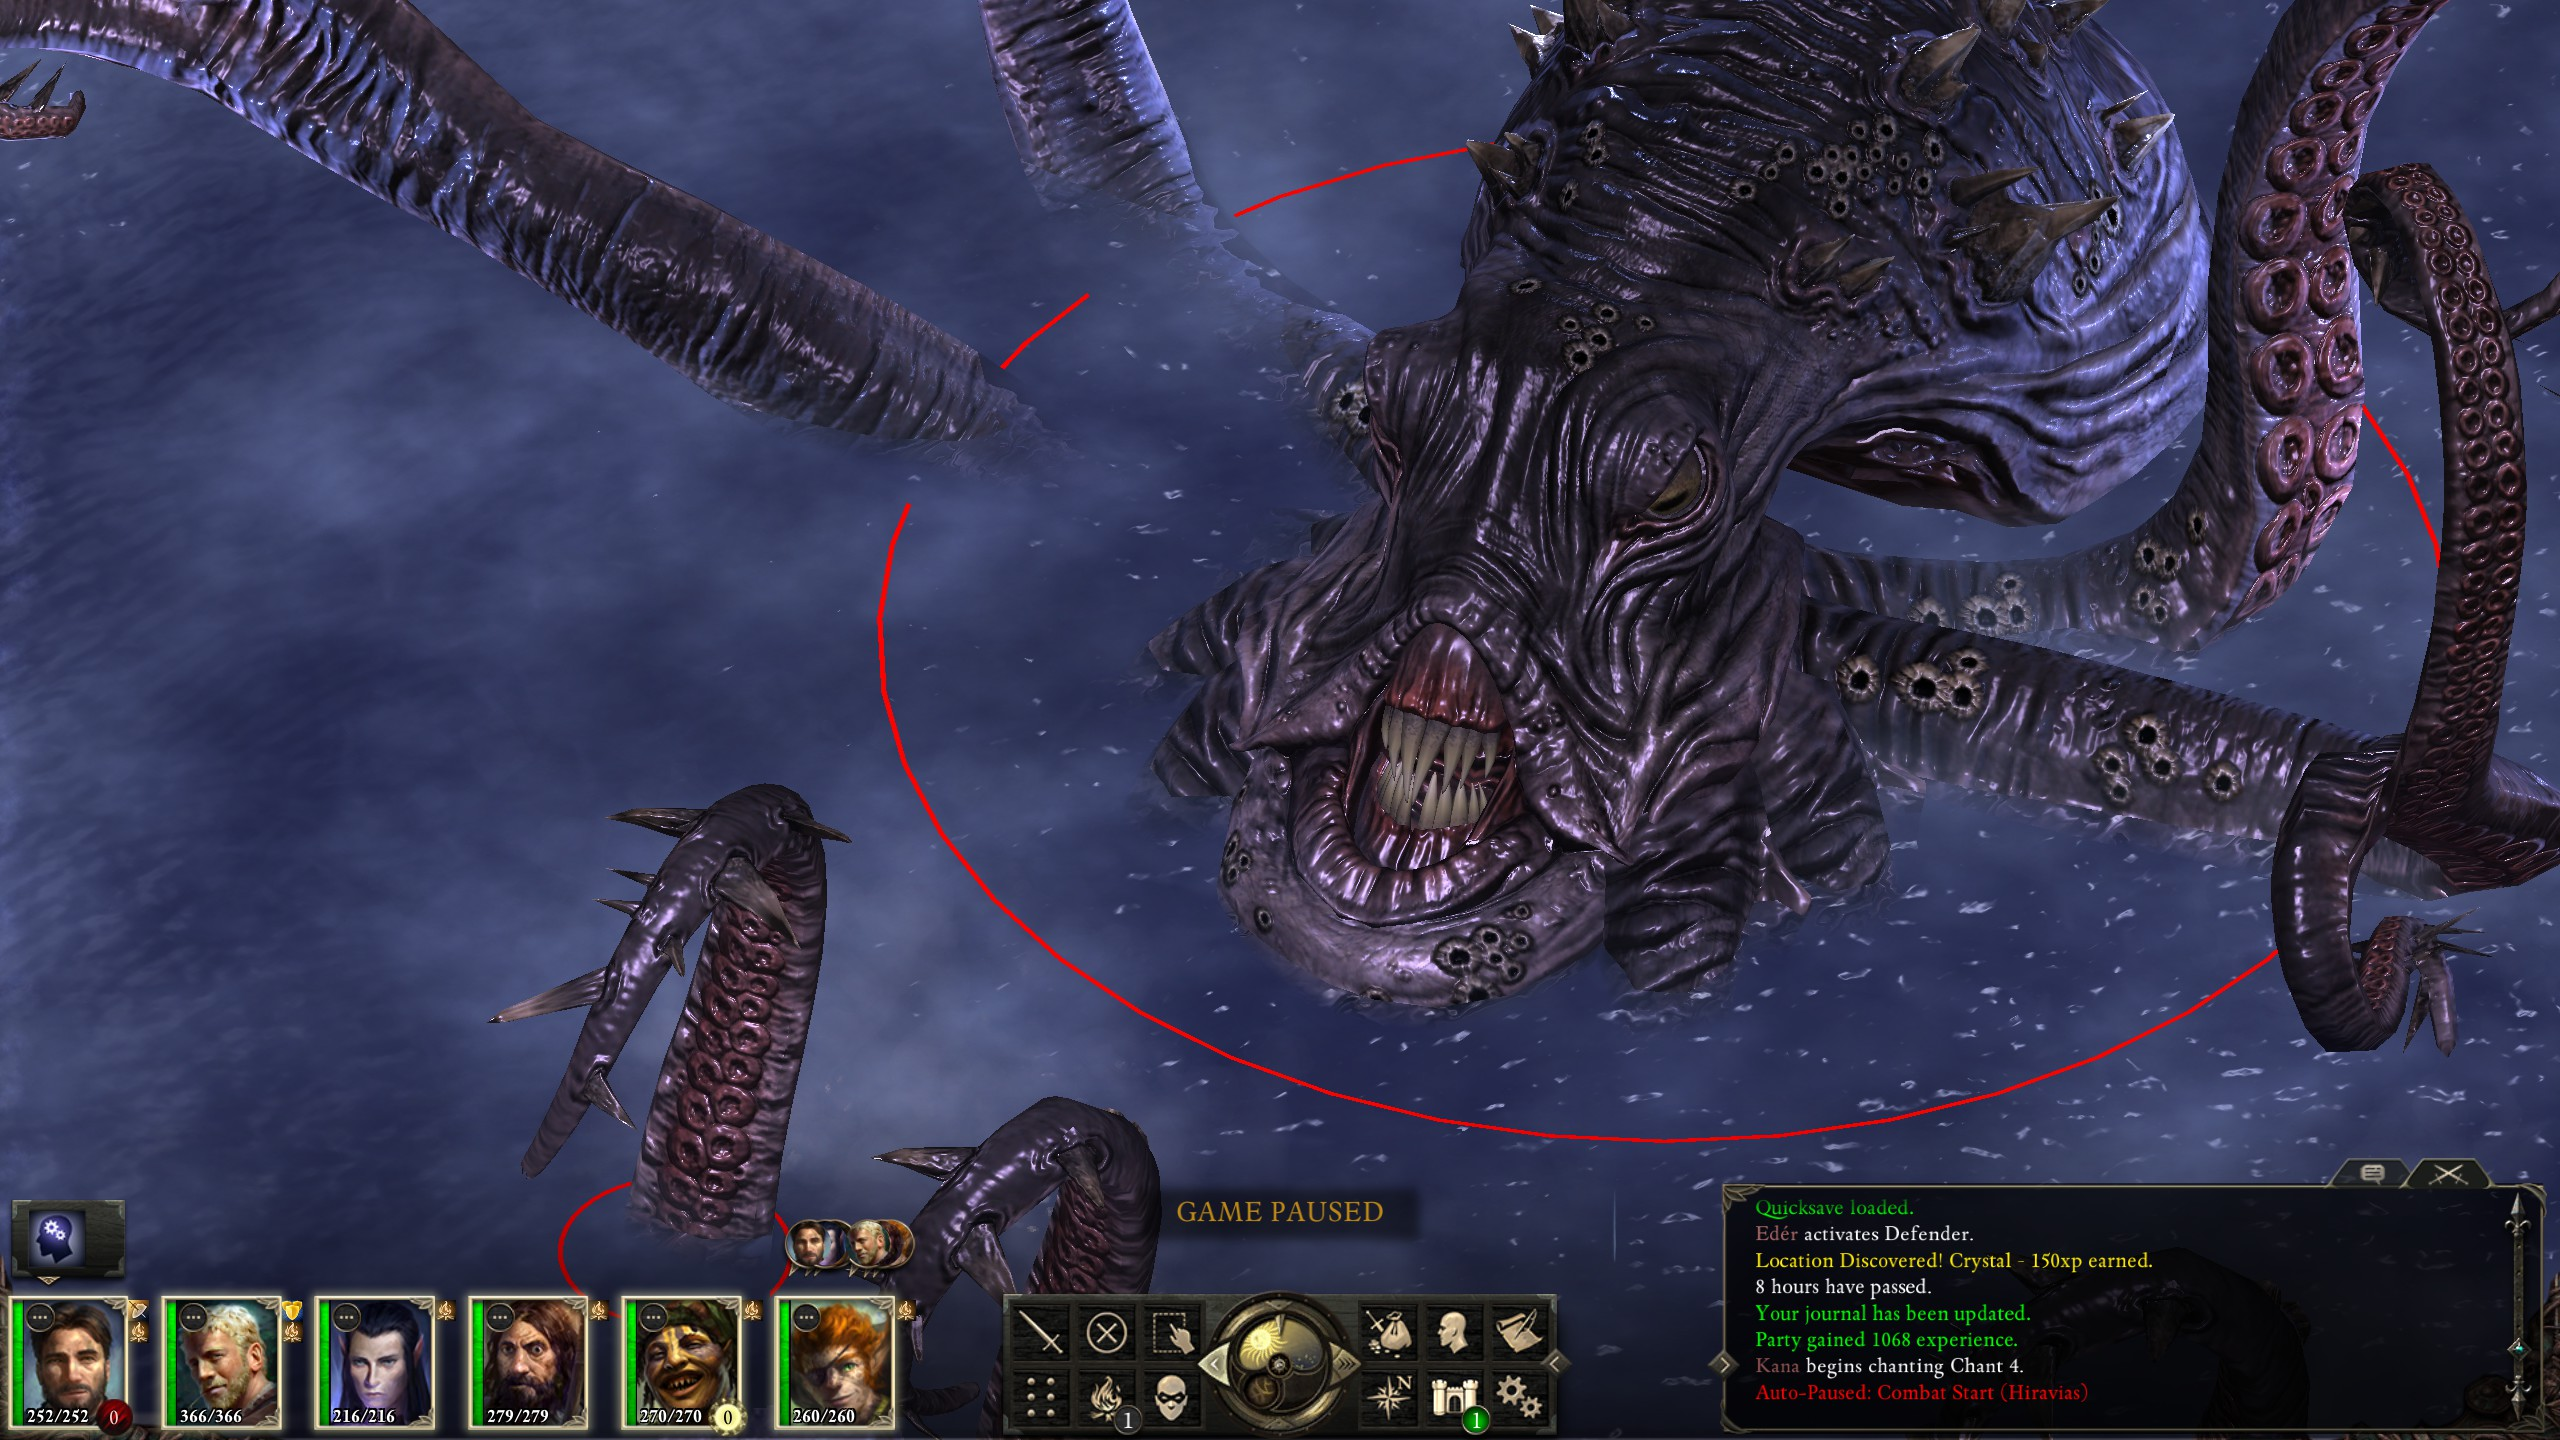
\includegraphics[scale=0.33]{files/blog/2020_01_18_poe_potd_wmpt2/2020_01_18_cayron2.jpg}
\end{figure}

I forgot to take any cool pictures of the fight but, sadly, the fight was quite easy.  The main reason for this is that the boss moved all of its tentacles towards me at the beginning of the fight where the boss was then out of range for any of its abilities.  This gave me time to buff up and kill the tentacles before charging with full power at the rather squishy boss.  Three eyeless then showed up right as the kraken died, but they were easily put down as well.  Once the boss was dead I then sunk the glacier and made it to safety using one of the two diving helmets I'd acquired from the various quests.

\begin{figure}
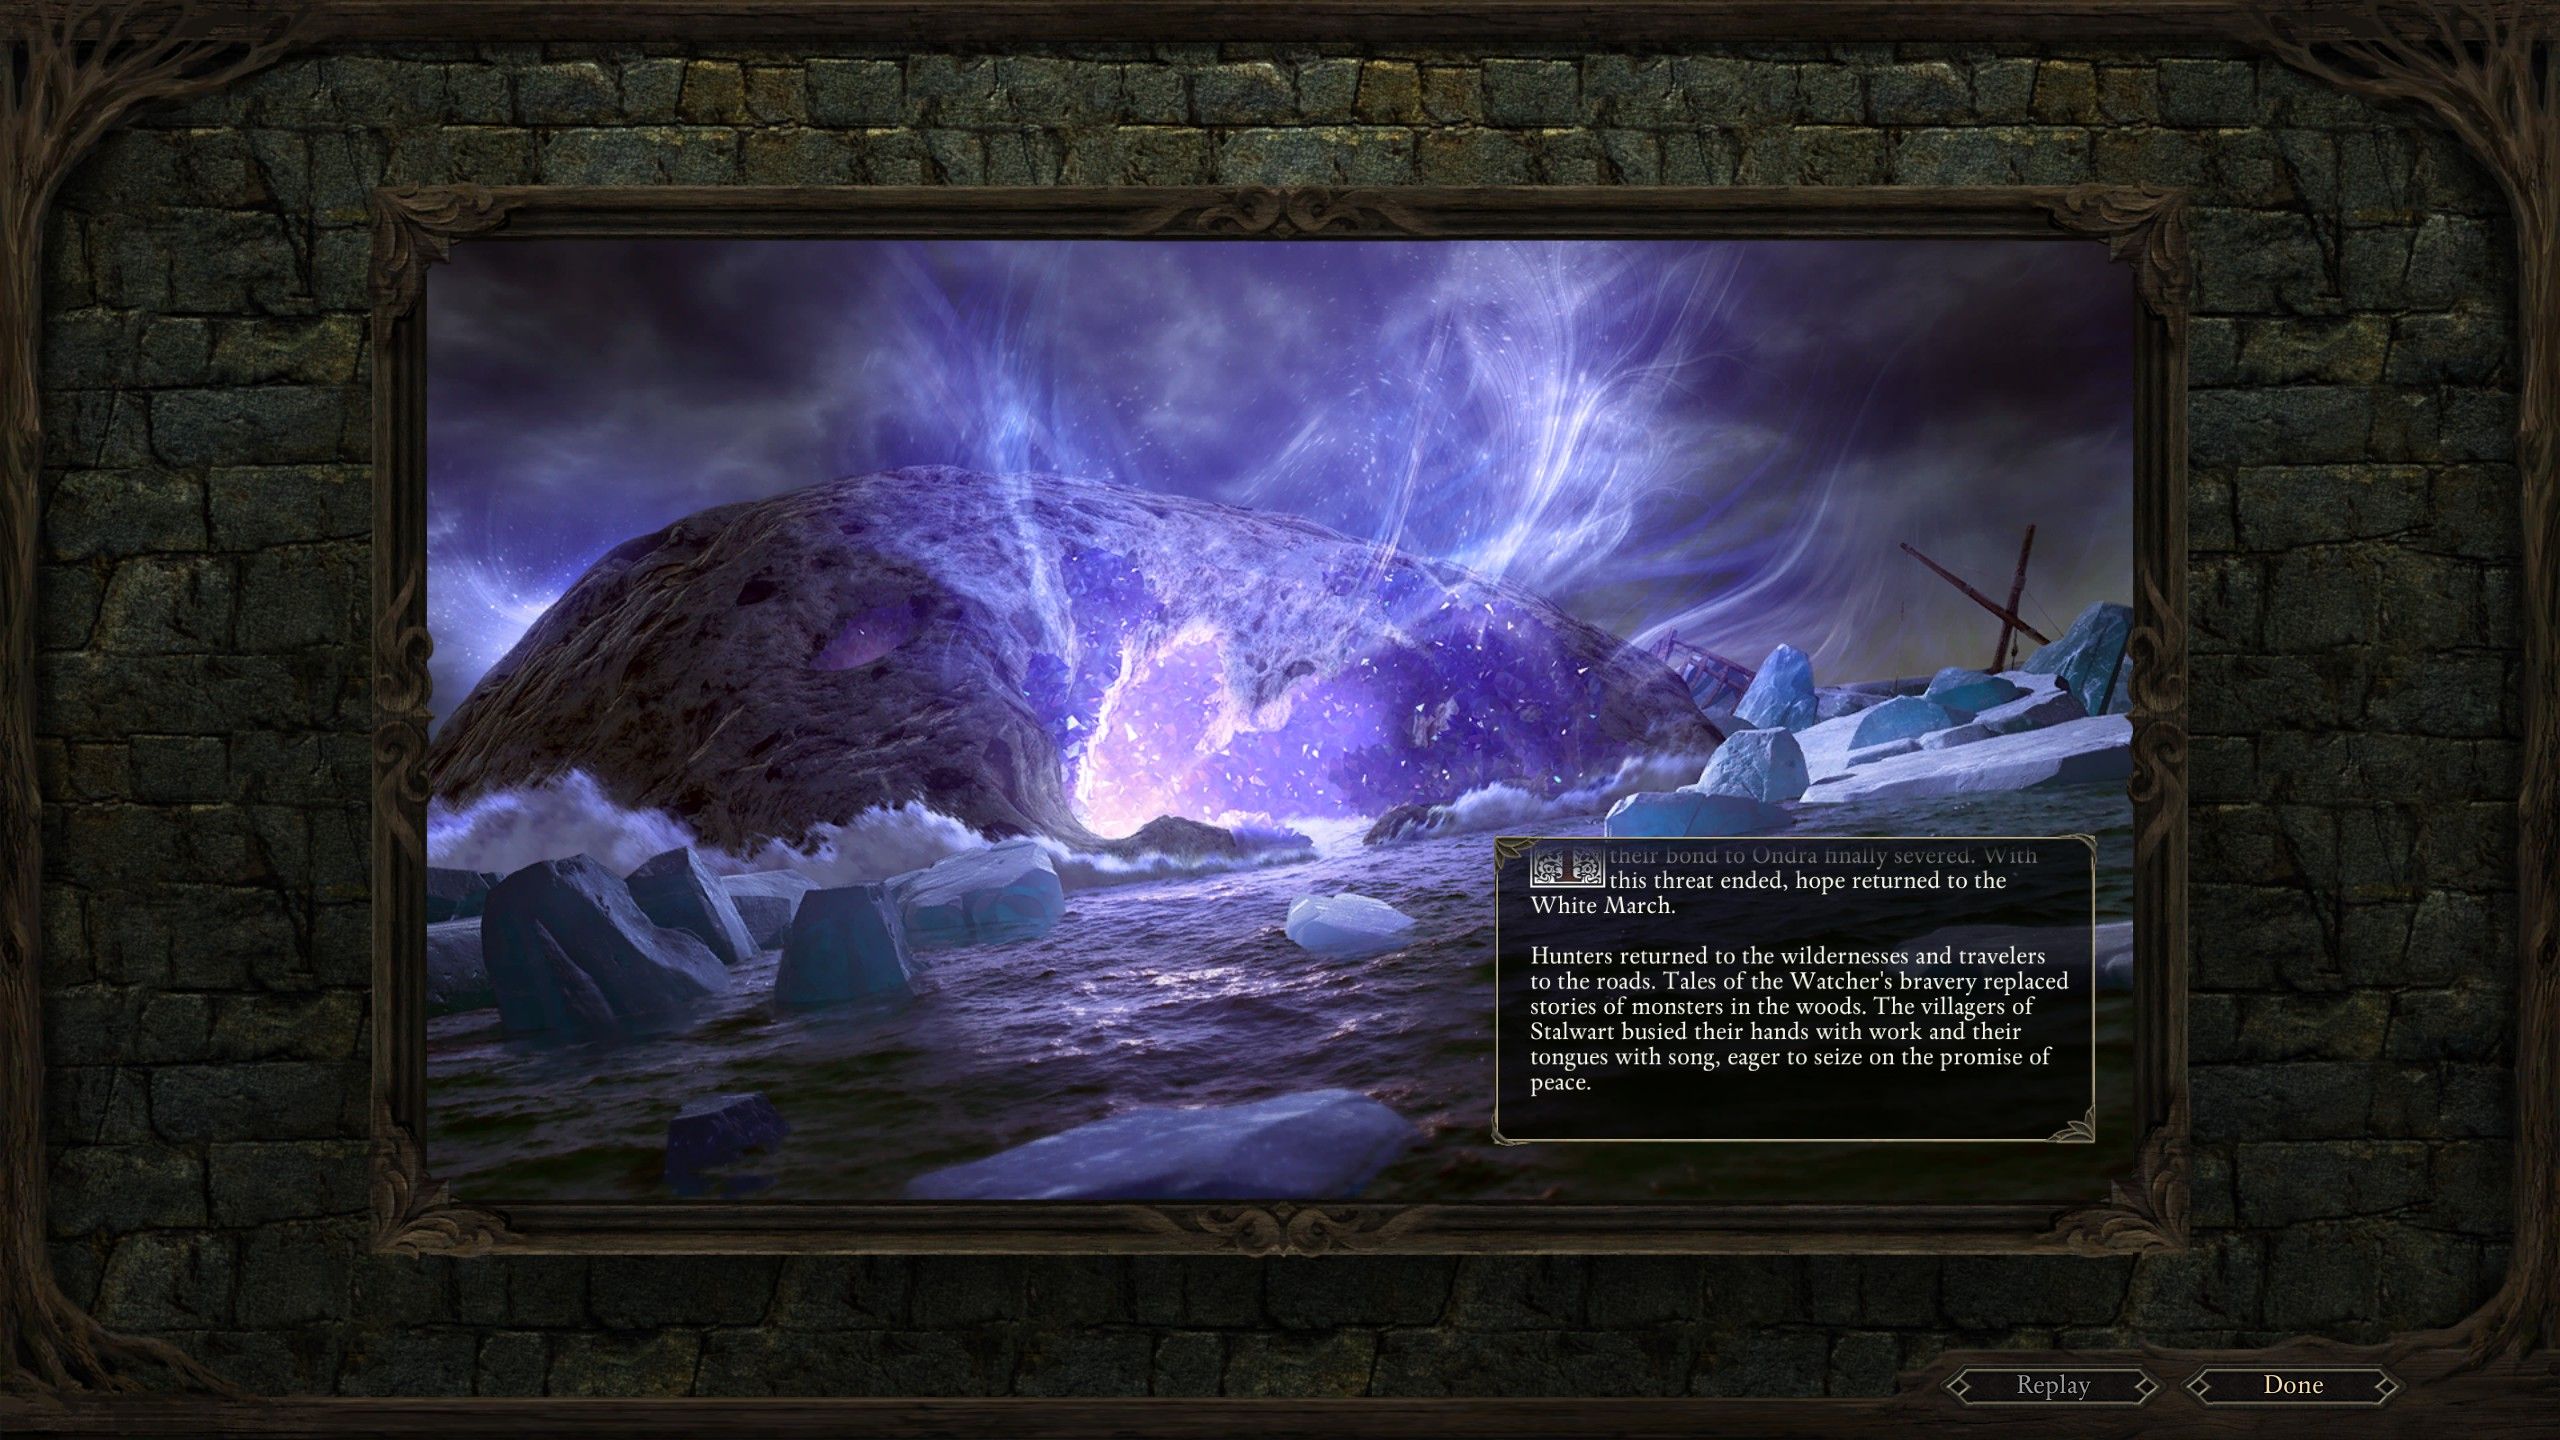
\includegraphics[scale=0.33]{files/blog/2020_01_18_poe_potd_wmpt2/2020_01_18_cayron3.jpg}
\end{figure}

That was the end of the expansion's main storyline, but not the optional endgame content in the bog, which is where I went next.

\subsection{The Bog}
The last and final level is actually a remote bog.  Ruins of engwith civilization lie all around, making for some interesting speculation regarding what this location might have once been used for.

\begin{figure}
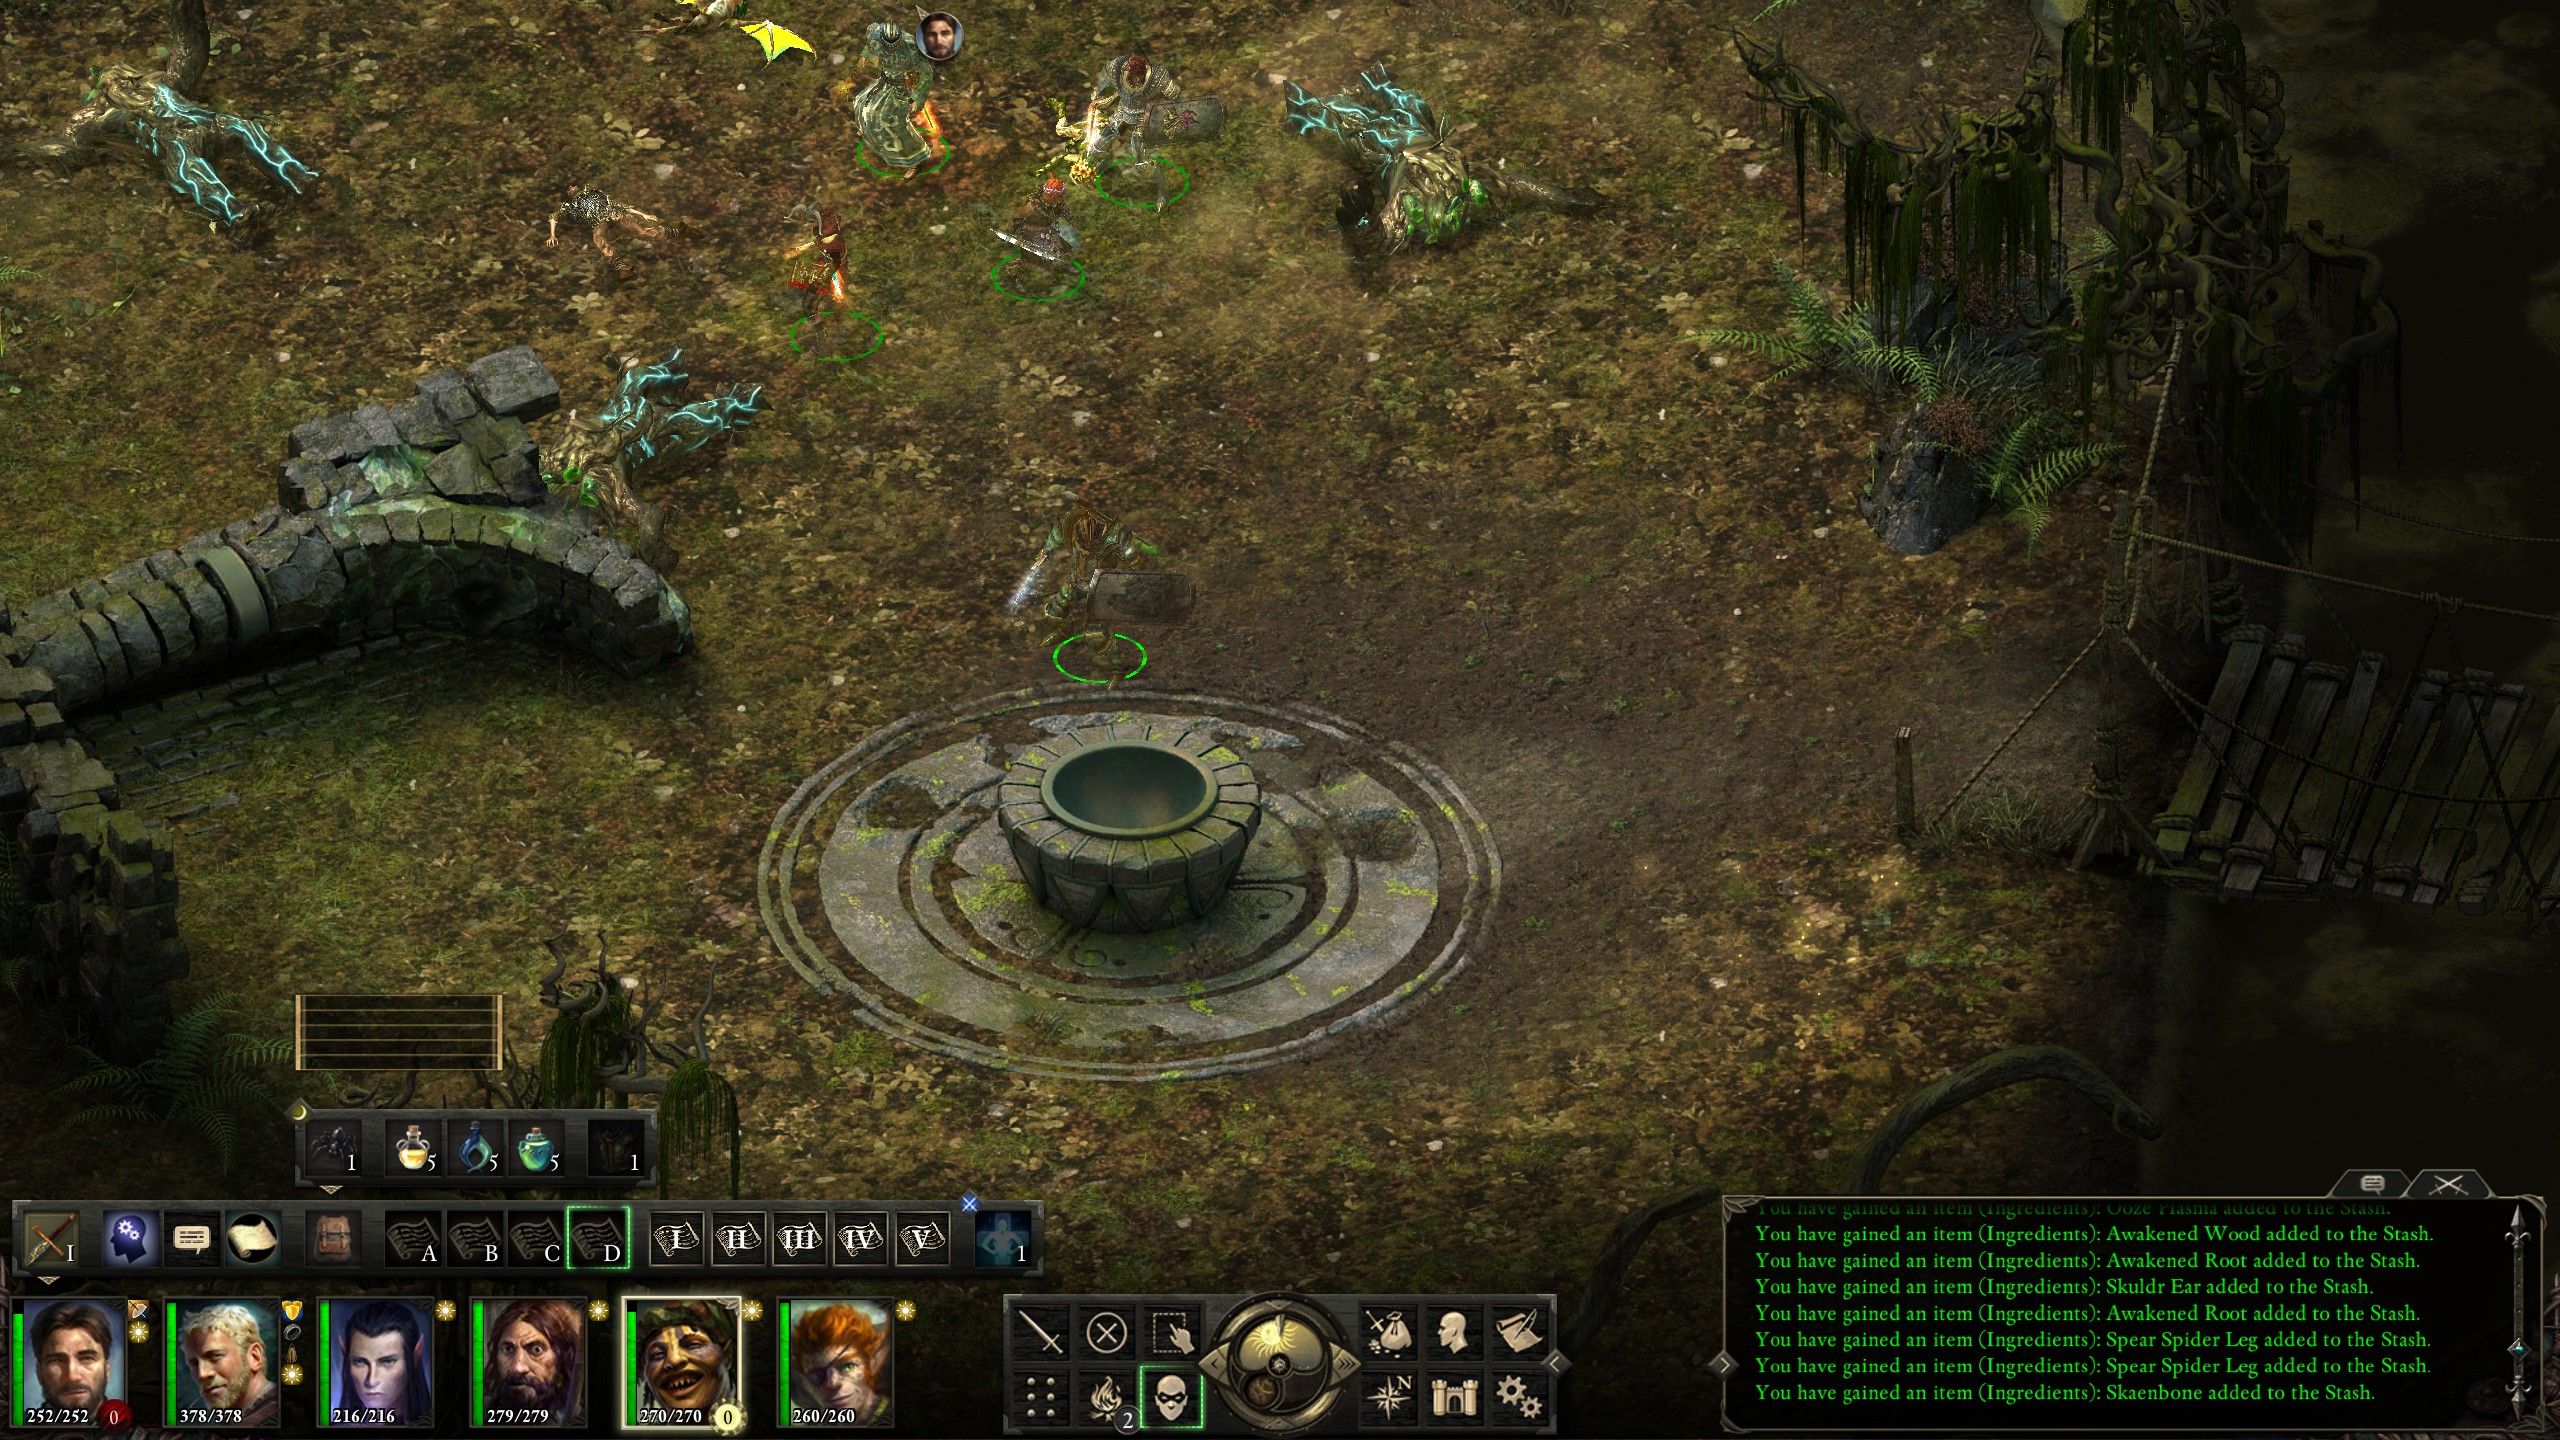
\includegraphics[scale=0.33]{files/blog/2020_01_18_poe_potd_wmpt2/2020_01_18_bog1.jpg}
\end{figure}

This giant head, for example, perhaps it served a similar purpose to that as the statue of Od Nua?

\begin{figure}
\includegraphics[scale=0.33]{files/blog/2020_01_18_poe_potd_wmpt2/2020_01_18_bog2.jpg}
\end{figure}

Alas, the ruins did not give any clue as to their original intent.

\begin{figure}
\includegraphics[scale=0.33]{files/blog/2020_01_18_poe_potd_wmpt2/2020_01_18_bog3.jpg}
\end{figure}

Neither did the bog cultists, for that matter.  Though I did have an issue where one of them managed to petrify my monk and do some serious damage, a lucky shot!  They didn't cause much trouble beyond that, though.

\begin{figure}
\includegraphics[scale=0.33]{files/blog/2020_01_18_poe_potd_wmpt2/2020_01_18_bog4.jpg}
\end{figure}

Beyond the bog cultists lay the final boss battle.

\subsubsection{Llengrath}
Upon entering the final area of the bog, a cultist blew a horn, summoning a dragon from the bog.  ``No problem'', I thought the first time this happened, ``I've fought a dragon before''.  Shortly after, \emph{another} dragon flew in with the archmage Llengrath atop it.

\begin{figure}
\includegraphics[scale=0.33]{files/blog/2020_01_18_poe_potd_wmpt2/2020_01_18_llengrath0.jpg}
\end{figure}

This was no ordinary dragon fight.  However, each individual dragon wasn't as tough as some of the other dragons I'd fought, such as the Adra Dragon or even the Alpine Dragon.  Since the enemies were far away, I began by staying in the back and buffing myself up.

\begin{figure}
\includegraphics[scale=0.33]{files/blog/2020_01_18_poe_potd_wmpt2/2020_01_18_llengrath1.jpg}
\end{figure}

In order to buy more time for buffs, I had each character use their summoning trinkets in order to create a defensive wall of minions in front of me while I prepared.

\begin{figure}
\includegraphics[scale=0.33]{files/blog/2020_01_18_poe_potd_wmpt2/2020_01_18_llengrath2.jpg}
\end{figure}

By the time I did engage the enemies, I was very powerful.  To my added amusement, Aloth's ``Wall of Many Colors'' actually managed to dominate the dragon Gafonercos, turning him against his allies and greatly increasing my odds of winning.

\begin{figure}
\includegraphics[scale=0.33]{files/blog/2020_01_18_poe_potd_wmpt2/2020_01_18_llengrath3.jpg}
\end{figure}

When dominate wore off, I took advantage of the petrified and paralyzed afflictions from the wall in order to deal massive damage to him and kill him.

\begin{figure}
\includegraphics[scale=0.33]{files/blog/2020_01_18_poe_potd_wmpt2/2020_01_18_llengrath4.jpg}
\end{figure}

With one dragon down, I set my fiery stag on the remaining enemies, surrounded Llengrath with Kana's summoned ogres, and cast ``Concelhaut's Crushing Doom'' on the dragon Turisulfus.

\begin{figure}
\includegraphics[scale=0.33]{files/blog/2020_01_18_poe_potd_wmpt2/2020_01_18_llengrath5.jpg}
\end{figure}

They did not last long after that.

\begin{figure}
\includegraphics[scale=0.33]{files/blog/2020_01_18_poe_potd_wmpt2/2020_01_18_llengrath6.jpg}
\end{figure}

In actuality, I found that the fight was pretty easy no matter the difficulty I played it on.  Llengrath seems to have mostly defensive spells, and the dragons seem weaker than the other standalone dragons.  After looting the bodies, I treated my monk to the highest possible enchantment for his civilian clothing.

\begin{figure}
\includegraphics[scale=0.33]{files/blog/2020_01_18_poe_potd_wmpt2/2020_01_18_llengrath7.jpg}
\end{figure}

Legendary clothing!  Though I've yet to figure out what exactly -15\% recovery speed means on armor with a recovery speed of 0\%.  -15\%, perhaps?

\subsection{The End}

That's pretty much a wrap.  Being a completionist, I did a quick vanity run through the actual endgame with Thaos and then relaxed by watching the epilogue and credits at normal speed as a celebration.  Below is a screenshot of some of the backers.

\begin{figure}
\includegraphics[scale=0.33]{files/blog/2020_01_18_poe_potd_wmpt2/2020_01_18_credits.jpg}
\end{figure}

I wonder if any of them will ever end up reading this blog?  Probably not.

Now, it is finally time for me to play the sequel, though I intend to import the save for my original run through of the game, mistakes and all, rather than the polished save that I created from this run.  I'm looking forward to seeing how my original choices play out in the sequel.


% A Brief Commentary on The Gulag Archipelago
\section{2020-01-05 A Brief Commentary on "The Gulag Archipelago"}
The quote on the back of my copy of Volume I of Solzhenitsyn's work, ``The Gulag Archipelago''\footnote{Solzhenitsyn, Aleksandr. \textit{The Gulag Archipelago: An Experiment in Literary Investigation}.  Harper Perennial, 2007.}, describes the work as, ``The greatest and most powerful single indictment of a political regime ever to be leveled in modern times\ldots'', but, when I read the book, I found it to be not just an indictment of the Soviet Union's particular political regime, but an indictment of Communist ideology itself.  Solzhenitsyn describes not just the atrocities committed by the Soviet Union, but also how the atrocities came about as a \emph{result} of Communist ideology.  This conclusion may be surprising to readers, as Marxism is often presented as as ideology of \emph{compassion}; indeed, the cover for a copy of ``The Communist Manifesto'' which I recently checked out for study has as its cover a picture of a \htmladdnormallink{little spinner}{https://en.wikipedia.org/wiki/File:No_Known_Restrictions_A_little_spinner_in_Globe_Cotton_Mill._Augusta,_Ga.,_by_Lewis_W._Hine,_1909_(LOC).jpg} factory worker.  Where, then, is the disconnect?  Why is it that an ideology that's seen as one of compassion should turn out to be so cruel?  I will attempt to answer these questions in this blog post.

First, it must be understood what the ``Gulag Archipelago'' is.  In the western republics, criminals are tried in a public \emph{court} and, if convicted, are sent to \emph{prisons} where they are, generally speaking, often idle.  In the Soviet Union, criminals go through an \emph{interrogation}, and, if convicted (in a \emph{private} court), are sent to a \emph{concentration camp} where they are made to do forced labor for the benefit of the state; along with this system of camps, there are a series of transit prisons and jails for holding those convicted, called \emph{zeks} in camp slang.  This system is dubbed the gulag \emph{archipelago} because the infrastructure is spread out across the Soviet Union like a series of small islands.  One article of the criminal code is particularly important to understanding the gulag: \emph{Article 58}, which dealt with ``crimes against the state'' and was used broadly in order to prevent any sort of opposition to Soviet power; those convicted under Article 58 (called simply \emph{58s} for short) were considered by the state to be common criminals rather than political prisoners, despite the political nature of the conviction.

The camps were both a means of political oppression\footnote{Vol. II, p578} via mass terror\footnote{Vol. I, p353} and a source of slave labor for the state.  This source of slave labor was needed by the state for all of the degrading, difficult, and dangerous work which free citizens were not willing to perform under socialism and which could not justifiably be rewarded with capitalist incentives\footnote{Vol. II, p578--579}.  What made the Soviet form of slave labor particularly hostile to human life and decency was the \emph{penalty ration}; zeks who did not complete the amount of work demanded of them by the state would receive less to eat\footnote{Vol. II, p78}.  Having the zeks sit idle in a cell was considered ``forced parasitism'', while making them work was in keeping with the Soviet Constitution: ``He who does not work does not eat''\footnote{Vol. II, p13-14}.  In practice, this meant exploiting the zeks by slowly starving them to death while profiting from their labor.

Within the gulag are many stories of calculated cruelty in addition to that of the ration system itself; to repeat all of the stories here verbatim would quickly dwarf the size of my writings.  As such, I will repeat a select few stories as appropriate throughout this blog.  I will organize the blog itself by explaining how the Soviets treated certain \emph{classes} of people on the basis of Communist ideology, then I will analyze the patterns that I see emerging, drawing comparisons \& and sometimes contrasting the Soviet regime with the regime to which I belong, that of the United States.  By attempting to emphasize the connections between the aspects of the Soviet system which were influenced by Communism rather than particular flaws of the Soviets themselves, it is my hope that this analysis will help to explain why Communism does not actually result in a more compassionate society and why the Soviet system was likely not an atypical implementation of Communism, and was therefore real Communism.

\subsection{The Classes in Gulag}
At the heart of the Communist ideology is its \emph{class theory}, which views human history as a history of \emph{class struggle}.  It should be no surprise, then, that those in gulag would consist in large part of those classes which were deemed \emph{oppressive}.  That, and the \emph{blatn\'{y}e}: a class belonging to a specific underworld subculture or ``law'' of thieves\footnote{Vol. I, p618 (Translator's Notes)}; these are people who practiced murder, rape, and robbery as part of their culture, and are referred to as simply \emph{thieves} throughout the translation and in this blog.  These thieves and the other zeks were then mixed based on the Communist principles of class struggle.

\subsubsection{Thieves}
\begin{quote}
Every crime is the result of a given social system\ldots

--- Comrade Krylenko, quoted in Vol. I, p319
\end{quote}

The Communists embraced idea that criminal activity results from class-based societies such as Capitalism\footnote{Vol. II, p432}, and they believed that their progressive society would be crime-free; after all, since crime resulted from classes, it was concluded that thieves were taught how to steal from their class enemies\footnote{Vol. II, p306} (believers, intellectuals, engineers, \&c.).  As the writer Gorky was quoted, ``\ldots any capitalist steals more than all of you combined!''\footnote{Vol. II, p93}.  In order to transition into the new, crime-free society, the Soviets developed a concept for their penal system which they called the \emph{reforging} of the thieves\footnote{Vol. II, p67}; Soviet jurist Averbakh is quoted by Solzhenitsyn explaining the prison regimen as such: ``The tactic of re-education is based on class differentiation\ldots~based on the strata friendliest to the proletariat''\footnote{Vol. II, p305} .  The idea of the thieves being a \emph{friendly} strata came from the fact that the thieves were also enemies of private property, and it was concluded that the thieves therefore merely needed to be guided into the political consciousness of the Soviets\footnote{Vol. II, p427}.  Solzhenitsyn thus explains the regime in detail:

\begin{quote}
Professional criminals can in no sense be equated with capitalist elements (i.e., engineers, students, agronomists, and ``nuns''), for the latter are steadfastly hostile to the dictatorship of the proletariat, while the former are only (!) politically unstable!  (A professional murderer is \emph{only} politically unstable!)  The lumpenproletarian is not a property owner, and therefore cannot ally himself with the hostile-class elements, but will much more willingly ally himself with the proletariat\ldots~That is why in the official terminology of Gulag they are called \emph{socially friendly} elements.  \ldots~That is why the regulations repeated over and over again: \emph{Trust} the recidivist criminals!  That is why through the Culture and Educational Section a consistent effort was supposed to be made to explain to the thieves the unity of their class interests with those of the workers, to indoctrinate them in a ``suspicious and hostile attitude toward the `kulaks' and counterrevolutionaries,'' and the authorities were to ``\emph{place their hopes} in these attitudes''!

--- Vol. II, p434
\end{quote}

This tactic of reforging based on class theory played out in the gulag such that thieves were given the top positions in the labor camps while the other prisoners were explicitly denied such positions\footnote{Vol. II, p469}, and the thieves were used against the ``socially hostile'' class elements by the Communists\footnote{Vol. II, p387--388} \footnote{Vol. III, p289--290}.

Solzehenitsyn describes his first encounter with the thieves as such:

\begin{quote}
You see cruel, loathsome snouts,\ldots~wearing expressions of greed and mockery.  Each of them looks at you like a spider gloating over a fly.  Their web is that grating which imprisons you---and you have been had!  They squinch up their lips, as if they intend to bite you from one side.  They hiss when they speak, enjoying that hissing more than the vowel and consonant sounds of speech\ldots~Their sinewy purple necks, their swelling shoulder muscles, their swarthy tattooed chests have never suffered prison emaciation.  \ldots~And suddenly you see a small cross dangling from one of those necks.  Yes, a little aluminum cross on a string.  You are surprised and slightly relieved.  That means there are religious believers among them.  How touching!  So nothing terrible is going to happen.  But immediately this ``believer'' belies both his cross and his faith by cursing,\ldots~and he jabs two protruding fingers, spread into the ``V'' of a slingshot, right in your eyes---not even pausing to threaten you but starting to punch them out then and there.  And this gesture of theirs, which says, ``I'll gouge out your eyes, crowbait!'' covers their entire philosophy and faith!

--- Vol. I, p502
\end{quote}

Solzhenitsyn later had his bundles of bacon, sugar, and bread stolen by the thieves while in the transit prison\footnote{Vol. I,p547--549}, but that was hardly the worst that could happen:

\begin{quote}
In 1946, retired Colonel Lunin, a high-ranking official in Osoaviakhim\ldots~recounted in a Buturki cell how the thieves in a Moscow Black Maria, on March 8, International Women's Day, during their transit from the City Court to Taganka Prison, gang-raped a young bride in his presence (and amid the silent passivity of everyone else in the van).  That very morning the girl had come to her trial a free person, as attractively dressed as she could manage (she was on trial for leaving her work without official permission---which in itself was a repulsive fabrication worked up by her chief in revenge for her refusal to live with him).  A half-hour before the Black Maria, the girl had been sentenced to five years under the decree and had then been shoved into this Black Maria, and right there in broad daylight, somewhere on the Park Ring ("Drink Soviet Champagne!"), had been turned into a camp prostitute.  And are we really to say that it was the thieves who did this to her and not the jailers?  And not her chief?

And thief tenderness too!  Having raped her, they robbed her.  They took the fashionable shoes with which she had hoped to charm the judges, and her blouse---which they shoved through to the convoy guards, who stopped the van and went off to get some vodka and handed it in so the thieves could drink at her expense.

And when they got to the Taganka Prison, the girl sobbed out her complaint.  And the officer listened to her, yawned, and said: ``The government can't provide each of you with individual transportation.  We don't have such facilities.''

--- Vol. I, p529--530
\end{quote}

Marxist compassion!  The class enemies who stood by silently and passively did not interfere in part because they were fearful of being stabbed; for a class enemy, to have a knife would be terrorism, but the thieves simply didn't know any better\footnote{Vol. I, p504} (and is this so far from our school supervisors who refuse to punish bullies because the bullies do not know any better?  Compassion as a virtue!  \ldots and what of Justice?).

These thieves, so favored by the Communists are, as Solzhenitsyn points out, the same as the pirates, the privateers, and freebooters, ``fascinating in romantic literary portraits\ldots~why are they so repulsive to you here?''\footnote{Vol. I, p515--516}, and, furthermore, ``\ldots has not all of world literature glorified the thieves?'' (``Pirates of the Carribean'', perhaps?).  Solzhenitsyn describes them in detail; tattoos such as ``\ldots a droll stoker hurling coal into their rear orifice\ldots''\footnote{Vol. I, p441}, stories of ``\ldots the luxurious life which the hero always had to achieve in the end\ldots''\footnote{Vol. II, p443} (\htmladdnormallink{sounds}{https://www.youtube.com/watch?v=zqflC-as2Qo} \htmladdnormallink{familiar}{https://www.youtube.com/watch?v=xX-N3B8ulnI}), and their slogan: ``you today, me tomorrow''\footnote{Vol. I, p145}.  This last point deserves further elaboration, and Solzhenitsyn describes their philosophy:

\begin{quote}
\begin{enumerate}
\item I want to live and enjoy myself; and fuck the rest!
\item Whoever is the strongest is right!
\item If they aren't fucking you, then don't lie down and ask for it.  (In other words; As long as they're beating up someone else, don't stick up for the ones being beaten.  Wait your own turn.)
\end{enumerate}

--- Vol. II, p428 (uncensored)
\end{quote}

What I find most striking about this philosophy is how \emph{rational} it is.  Is #1 not the guiding principle behind the ``I've got mine!'' political attitude?  #2 is a clear-cut case of Darwinian Selection, so the thieves have not lagged \emph{behind the times} with an \emph{irrational}, superstitious faith in Justice.  And is principle #3 not taught at our Universities, except there it's called the Prisoner's Dilemma and explained in less obviously profane terms (but is the end result not the same)?

Going back to the Soviets and their reforging, it appears that the thieves taught the Soviets rather than vice-versa.  Solzhenitsyn explains of how, during inter-prison \& camp transport in a Stolypin railcar, the convoy guard would intentionally mix a few thieves into each cell so that the thieves would plunder the class enemies, then pawn the things off to the guard in exchange for rations, vodka, tobacco, \&c.\footnote{Vol. I, p507}.  In one case where there were no thieves on board to plunder the class enemies, the guard lowered the prisoners' rations until the prisoners sold their stuff to the convoy for the rations\footnote{Vol. I, p506--512}.  The thieves, however, were not as keen to acquire the official's traits:

\begin{quote}
The urka---the habitual thief---who adopted the Chekist faith became a \emph{bitch}, and his fellow thieves would cut his throat.  The Chekist who acquired the psychology of the thief was an \emph{energetic} interrogator of the thirties and forties, or else a \emph{resolute} camp chief---such men were appreciated.  They got the service promotions.

--- Vol. II, p428
\end{quote}

The psychology did not stay confined to the gulag, though, and was transmitted from there via \emph{campside} (the areas adjacent to the gulag) to undergo trial and selection for transmission to the broader Soviet Union\footnote{Vol. II, p564--565}.  Perhaps beyond, too; I've personally found the thief word ``tukhta'' (padding of the books) to be useful when referring to employer metrics, and is that not a result of ``diversity'' of culture?

Despite its basis in Communist class theory, the Soviet's social system and prison regime did not reforge the thieves as they had predicted.  In the early fifties, when the thieves had gotten out of control, the administration played the bitches against the thieves\footnote{Vol. II, p421--422}; this was known as the ``bitches' war''\footnote{Vol. III, p243--244}.  Likewise, Stalin himself started putting the ringleaders of the thieves in prison\footnote{Vol. II, p478} or isolators\footnote{Vol. II, p445--446} rather than camp.  The thieves were still intentionally used by the Soviets against their class enemies\footnote{Vol. III, p289}, but the promise of reforging the thieves had failed.

\subsubsection{Christians}
\begin{quote}
Religion is the opiate of the masses.

--- Karl Marx
\end{quote}

There seems to me to be a growing trend to view Christianity as the ``oppressor religion'' (and, indeed, I had adopted this view in the past).  This idea was tried thoroughly with Soviet Russia's state atheism, which persecuted believers for their faith.  According to prosecutor Comrade Krylenko, the clergy were all ``class enemies''\footnote{Vol. I, p323}, and accuser Krasikov exclaimed, ``The whole Orthodox Church is a subversive organization.  Properly speaking, \emph{the entire church ought to be put in prison}.''\footnote{Vol. I, p351}.  The problem was that, rather than always following the \emph{dictatorship} of the workers, the believers would refuse to act in a manner contrary to their morality; as Patriarch Tikhon explained: ``I recognize \verb|[|the state's laws\verb|]|, \emph{to the extent that they do not contradict the laws of piety}.''\footnote{Vol. I, p348}.  Judge Bek thus made the accusation against Patriarch Tikhon: ``propaganda is an attempt to prepare a mood preliminary to preparing a \emph{revolt} in the future.''\footnote{Vol. I, p349}; that is to say that anything that contradicted state doctrine was \emph{counter-revolutionary} and therefore a crime.  The idea that individuals might make a conscious moral decision differing from the demands of state law of their own free will was not respected by the dictatorship.  As such, the believers had to be \emph{re-educated}, as Solzhenitsyn writes:

\begin{quote}
Believers must be dismissed from their jobs merely for their faith; Komsomols must be sent along to break the windows of believers; believers must be officially compelled to attend antireligious lectures, church doors must be cut down with blowtorches, domes pulled down with hawsers attached to tractors, gatherings of old women broken up with fire hoses.  (Is this what you mean by \emph{dialogue}, French comrades?)

--- Vol. III, p514
\end{quote}

Other pressures included: requirements to violate the secrecy of the confessional by becoming informers for the state\footnote{Vol. I, p59}, refusing to work on Sundays being considered economic sabotage\footnote{Vol. I, p59}, and non-atheist communes having their teachers arrested for not following the government programs\footnote{Vol. I, p51}.  There are many notable stories of this persecution, such as: the banning of religious famine-relief programs (a famine in which cannibalism, even parents eating their own children, was practiced) followed by the forced requisition of all church valuables\footnote{Vol. I, p342--349}, the tracking down and arrest of an independent Yaruyevo commune\footnote{Vol. III, p366--367}, and starving a group of arrested old monks that refused to sign paperwork\footnote{Vol. II, p65--66}:

\begin{quote}
In the Summer of 1930 they brought to Solovki several dozen religious sectarians who rejected anything that came from the anti-Christ: they refused to accept any documents, including passports, and they refused to sign for anything or to handle any money.  At their head was a gray-bearded old man of eighty, blind and bearing a long staff.  Every enlightened person could clearly see that these sectarians could never ever enter into socialism, because that required having a great to deal to do with papers---and that therefore the best thing for them to do was to die.  And so they sent them off to Maly Zayatsky Island, the smallest in the entire Solovetsky archipelago---sandy, unforested desert, containing a summer hut of the former monk-fishermen.  And they expressed willingness to give them two months' rations, the condition being that \emph{each one} of the sectarians would have to sign for them on the invoice.  Of course they refused. \ldots~And so they were \emph{sent off without food}.  Two months later (exactly two months because they were then to be asked to sign for their food for the next two months) they sailed over to Maly Zayatsky and found only corpses which had been picked by the birds.  Everyone was there.  No one had escaped.

--- Vol. II, p66
\end{quote}

In the current-day United States there are many people who identify themselves as ``Christian'', yet a common question asks how many of them would have the willpower to stand by their convictions in the face of persecution?  This ambiguity does not exist for those believers imprisoned in the gulag because of their faith, as Solzhenitsyn writes:

\begin{quote}
The Tao says: When faith collapses, that is when the true believers appear.  Because of our enlightened scoffing at Orthodox priests\ldots~we overlooked the fact that the sinful Orthodox Church had nonetheless nurtured daughters worthy of the first centuries of Christianity---sisters of those thrown to the lions in the arenas.  \ldots~They were the best of Russia's Christians.  The worst had all\ldots~trembled, recanted, and gone into hiding.

--- Vol. II, p310
\end{quote}

The perserverance of these determined few is inspiring.  For example, one of the penalty camps where people wore \emph{numbers} instead of names, a sect of women believers refused to wear what they considered the mark of Satan, and so were stripped to their shifts and made to walk in sub-freezing temperatures (Marxist compassion!) until the administration gave up and returned them their old clothing without numbers, but refused to issue new clothing without a signed receipt\footnote{Vol. III, p67}.  Most telling, though, is how, despite camp administration threats, a belief in Christ was one of the few means available to avoid becoming an \emph{informer}\footnote{Vol. II, p373}, and Solzhenitsyn added poetically:

\begin{quote}
And does the impartial reader not find that \verb|[|the security officers\verb|]| flee from Christ like devils from the sign of the cross, from the bells calling to matins?

--- Vol. II, 374
\end{quote}

Contrast this steadfastness with those who truly believe that the ``rational'' choice of \emph{betrayal} in the Prisoner's Dilemma is the optimal one, and consider what \emph{kind} people they are\ldots~do they inspire admiration, or revulsion?  As Solzhenitsyn pointed out when stoolies began seeking shelter in the camp prison from their fellow prisoners who had begun knifing them (an event called \emph{the chopping}):

\begin{quote}
\ldots A stoolie is only wanted, only useful, so long as he can rub shoulders with the crowd and pass undetected.  Once detected, he is worthless, and cannot go on serving in the same camp.  He eats the bread of idleness in the Disciplinary Barracks, doesn't go out to work, isn't worth his salt.  Even the MVD's philanthropy must have some limits!

So the flow of stoolies begging to be saved was stemmed.  Late-comers had to remain in their sheep's clothing and await the knife.

An informer is like a ferryman: once he's served his purpose, nobody wants to know him.

--- Vol. III, p242
\end{quote}

The true believers, though, did not stoop to that level, and were persecuted by the Soviet dictatorship as result.

There is one final manifestation of the Soviet regime which I wish to include here, as I believe that it has symbolic significance.  Although the Soviets had destroyed the Christian monks, they found that the monasteries that they had built, with their strong, stone walls in isolated locations were still useful as \emph{prisons}\footnote{Vol. II, p19} \footnote{Vol. II, p28} \footnote{Vol. II, p74}.  Likewise, churches were turned into transit prisons\footnote{Vol. III, p361} (especially those in the actual prisons\footnote{Vol. I, p605}), but others were put to even less holy uses, as Solzhenitsyn writes:

\begin{quote}
In Pskov alone, the NKVD set up torture and execution chambers in the basements of many churches, in former hermits' cells.  And even in 1953 tourists were still not allowed into these churches, on the grounds that ``archives'' were kept there.  The cobwebs hadn't been swept out for ten years at a stretch: those were the ``archives'' they kept there.  And before beginning restoration work on these churches, they had to haul away the bones in them by the truckload.

--- Vol. I, p438
\end{quote}

So we can answer that question, ``\htmladdnormallink{Is all the world jails and churches?}{https://www.youtube.com/watch?v=7sqFprD6qIs}'' with a resounding, ``No!  In some places there are \emph{only} jails!''.

\subsubsection{Intelligentsia}
\begin{quote}
In actual fact \emph{they are not \verb|[|the nation's\verb|]| brains, but shit}.

--- Comrade Lenin, quoted in Vol. I, p328
\end{quote}

Comrade Lenin, Stalin's ``humane'' predecessor, had no love for the ``rotten-liberal''\footnote{Vol. I, p328} intelligentsia of Russia.  Although the intelligentsia were not bourgeois proper because they were not the land owners, they had \emph{worked for} the bourgeois and their \emph{ideas} were still bourgeois; Lenin therefore called them, ``a pitiful petty bourgeois, imprisoned in bourgeois prejudices''\footnote{Vol. I, p31}.  Much like the Christians were subject by the Soviets to re-education, the intelligentsia were subjected by the Soviets to \emph{re-evaluation}; they naturally found that the ideas held by the intelligentsia were lagging behind the times\footnote{Vol. I, p328}.  Not only that, but they were now considered as actively harmful, as Comrade Krylenko exclaimed:

\begin{quote}
The Russian intelligentsia which entered the crucible of the Revolution with slogans of power for the people emerged from it an ally of the black generals, and a hired and obedient agent of European imperialism.  The intelligentsia trampled on its own banners, and covered them with mud.

--- Comrade Krylenko, quoted in Vol. I, p328--329
\end{quote}

The Soviets claimed that the intelligentsia had ``betrayed the cause of the workers''\footnote{Vol. I, p328}.  For example:

\begin{quote}
Several dozen young people got together for some kind of musical evening which had not been authorized ahead of time by the GPU.  They listened to music and then drank tea.  They got the money for the tea by voluntarily contributing their own kopecks.  It was quite clear, of course, that this music was a cover for counterrevolutionary sentiments, and that the money was being collected not for tea but to assist the dying world bourgeois.  And they were \emph{all} arrested and given from three to ten years---Anna Skripnikova getting five, while Ivan Nikolayevich Varentsov and the other organizers of the affair who refused to confess were \emph{shot!}

--- Vol. I, p43
\end{quote}

Likewise, in the middle of the Civil War, the intelligentsia made works such as books, memoranda, and projects\footnote{Vol. I, p330}, and Comrade Krylenko thus scorned them: ``It was your duty to think first of all \emph{how you might die in battle}''\footnote{Vol. I, p332}.  Worse, they had written books about what \emph{kind} of system should replace the Soviet regime were it to fail.  Not only did they think that Soviet power might fail, but they wanted \emph{Democracy} rather than the Communist ideal: the \emph{dictatorship} of the workers.  This was unacceptable to the Soviets:

\begin{quote}
\ldots even a conversation over a teacup as to the kind of system that should replace the Soviet system, which is allegedly about to fall, is a counterrevolutionary act\ldots~During the Civil War not only is any kind of action \verb|[|against Soviet power\verb|]| a crime\ldots~but the \emph{fact of inaction is also criminal.}

--- Comrade Krylenko, quoted in Vol. I, p332
\end{quote}

Rather than \emph{thinking} and then sharing their \emph{ideas}, the Soviets demanded unwavering, unthinking loyalty to their dictatorship from the intelligentsia.  Since the intelligentsia did not provide this unwavering loyalty, the tribunal sentenced the defendants to be shot (Marxist compassion intervened, though, and the sentence ``was commuted to concentration camp until the end of the Civil War''\footnote{Vol. I, p331}).  As far as Krylenko was concerned, this was just:

\begin{quote}
The political instability and the interim nature of the intelligentsia\ldots~completely justified that Marxist evaluation of the intelligentsia made by the Bolsheviks.

--- Comrade Krylenko, quoted in Vol. I, p333
\end{quote}

Yet it is by their very nature that the intelligentsia are not capable of blind faith in any particular system, as Solzhenitsyn explains:

\begin{quote}
Over the years I have had much occasion to ponder this word, the \emph{intelligentsia}.  We are all very fond of including ourselves in it---but you see not all of us belong.  In the Soviet Union this word has acquired a completely distorted meaning.  They began to classify among the intelligentsia all those who don't work (and are afraid to) with their hands.  All the Party, government, military, and trade-union bureaucrats have been included.  All book-keepers and accountants---the mechanical slaves of Debit.  All office employees.  And with even greater ease we include here \emph{all} teachers (even those who are no more than talking textbooks and have neither independent knowledge nor an independent view of education).  \emph{All} physicians, including those capable only of making doodles on the patients' case histories.  And without the slightest hesitation all those who are only in the vicinity of editorial offices, publishing houses, cinema studios, and philharmonic orchestras are included here, not even to mention those who actually get published, make films, or pull a fiddle bow.

And yet the truth is that not one of these criteria permits a person to be classified in the intelligentsia.  If we do not want to lose this concept, we must not devalue it.  The intellectual is not defined by professional pursuit and type of occupation.  Nor are good upbringing and a good family enough in themselves to produce an intellectual.  An intellectual is a person whose interests and preoccupation with the spiritual side of life are insistent and constant and not forced by external circumstances, even flying in the face of them.  An intellectual is a person whose thought is nonimitative.

--- Vol. II, p281
\end{quote}

The Soviets, however, believed themselves to be on ``the right side'' of history and thus had no room for alternate ideas or deviant behaviors.  As shown above, anything but perfect obedience and conformity to the cause of the Soviets was not only going against the state's notions on the progression of history, but was actually criminal, thus the intelligentsia had no place in the new society and had ``outlived its time''\footnote{Vol. I, p329}.  In camp, the intelligentsia were destroyed:

\begin{quote}
\ldots the system of Corrective Labor Camps in particular, with their obligatory and exhausting physical labor and their obligatory participation in the humiliating, buzzing ant heap, was a more effective means of destroying the intelligentsia than was prison.  It was precisely the intelligentsia that this system killed off quickly and completely.

--- Vol. II, p631
\end{quote}

In this manner the intelligentsia was purged from the new, humanitarian society.

\subsubsection{Engineers}
\begin{quote}
The bourgeoisie has stripped of its halo every occupation hitherto honored and look up to with reverent awe.  \ldots~It has converted the physician, the lawyer, the priest, the poet, the man of science, into its paid wage laborers.

--- Karl Marx, as quoted by Solzhenitsyn, Vol. II, p256
\end{quote}

Which engineers, when concerned more with the integrity of their profession than pursuit of profit alone, do not feel on some level degraded by an avaricious Capitalist's demand for revenue over a quality product?  Their energy directed only towards their own short-term interests without account of the customer, the Capitalist's peoples, or the trade's integrity, what contempt they inspire!  Here Marx has voiced a similar contempt, implying that one might find solutions to this problem in a Communist system.

But, as with the intellectuals before, it turns out that the engineers are not ``workers'' but, as Solzenitsyn pointed out, merely ``lackeys and servants of former capitalist bosses''\footnote{Vol. I, p43}, and thus were also tainted by class corruption.  The engineers then had to be made to subservient to the ``real'' workers, as this passage illustrates:

\begin{quote}
\ldots while their superiors demanded successes in production from them, and discipline, they were deprived of the authority to impose this discipline.  Any worker could not only refuse to carry out the instructions of an engineer, but could insult and even strike him and go unpunished---and as a representative of the ruling class the worker was \emph{always right} in such a case.

--- Vol. II, p391
\end{quote}

Here again is the central theme of Communism: the \emph{dictatorship} of the workers.  Unsurprisingly, the engineers of Russia were not enthusiastic about their new rulers:

\begin{quote}
What the engineers had first seen in the October coup d'\'etat was ruin.  (And for three years there had truly been ruin and nothing else.)  Beyond that, they had seen the loss of even the most elementary freedoms.  (And these freedoms never returned.)  How, then, could engineers \emph{not have wanted} a democratic republic?  How could \emph{engineers} accept the \emph{dictatorship of the workers}, the dictatorship of their subordinates in industry, so little skilled or trained and comprehending neither the physical nor the economic laws of production, but now occupying the top positions, from which they supervised the \emph{engineers}?  Why shouldn't the engineers have considered it more natural for the structure of society to be headed by those who could intelligently direct its activity?

--- Vol. I, p390
\end{quote}

But Democracy is not the goal of Communism, and so such ideas were \emph{counter-revolutionary} and made the engineers as a class \emph{socially hostile}.  The threat to the engineers was not immediate after the revolution, as the engineers were still needed for production, but the new dictators did not trust the engineers who, ``\ldots had come to regard \verb|[|themselves\verb|]| as too irreplaceable and had not gotten used to catching instructions on the wing.''\footnote{Vol. I, p43} (am I getting \htmladdnormallink{D\'ej\`a vu}{https://feross.org/funding-experiment-recap/}?).  The atmosphere the old engineers faced is summarized nicely in a footnote:

\begin{quote}
They say that when Ordzhonikidze used to talk with the old engineers, he would put one pistol on his desk beside his right hand and another beside his left.

--- Vol. I, p45
\end{quote}

Since it was impossible to correct socially hostile prisoners due to their class corruption\footnote{Vol. II, p254}, the Communists' solution was to train a new generation of engineers in order to replace the old engineers.  As these new engineers began to emerge and the Five-Year Plans of the Communists' began to run into trouble, the old engineers' social hostility was exposed by their failures to meet the state plan, not because the plans were unrealistic, but because the old engineers were engaged in a form of sabotage known as \emph{wrecking}:

\begin{quote}
Nikolai Karlovich von Meck, of the People's Commissariat of Railroads, pretended to be terribly devoted to the development of the new economy, and would hold forth for hours on end about the economic problems involved in the construction of socialism, and he loved to give advice.  One such pernicious piece of advice was to increase the size of freight trains and not worry about heavier than average loads.  The GPU exposed von Meck, and he was shot: his objective had been to wear out rails and roadbeds, freight cars and locomotives, so as to leave the Republic without railroads in case of foreign military intervention!  When, not long afterward, the new People's Commissar of Railroads, Comrade Kaganovich, ordered that average loads should be increased, and even doubled and tripled them (and for this discovery received the Order of Lenin along with others of our leaders)---the malicious engineers who protested became known as \emph{limiters}.  They raised the outcry that this was too much, and would result in the breakdown of the rolling stock, and they were rightly shot for their lack of faith in the possibilities of socialist transport.

--- Vol. I, p45
\end{quote}

This story is a great summary of the engineer's predicament: every design decision involves trade-offs, so how could they possibly make a decision that can't be construed as wrecking?  In our oppressive Capitalist system, one weighs the costs and benefits of each decision before making it and, if the result displeases the bosses, that engineer may be fired; in an enlightened Communist system, a choice that displeases the bosses is \emph{criminal}, as failure to meet the five-year plans is a sign of criminal wrecking rather than ineptitude and/or laziness.  So now imagine the demands of avaricious Capitalist bosses, except failure to meet their demands now threatens one with the gulag (where labor would be credited to the camp, i.e. \emph{unpaid}).  Marxist compassion!

By design, the old engineers did not make it through the systematic purges (see the Oldenborger trial\footnote{Vol. I, p336} and the Promparty Trial\footnote{Vol. I, p376} for more examples), and they were eventually replaced with a new generation of engineers.  Having known both the old and the new engineers, Solzhenitsyn contrasts the two, starting by describing the old engineers:

\begin{quote}
I had grown up among engineers, and I could remember the engineers of the twenties very well indeed: their open, shining intellects, their free and gentle humor, their agility and breadth of thought, the ease with which they shifted from one engineering field to another, and, for that matter, from technology to social concerns and art.  Then, too, they personified good manner and delicacy of taste; well-bred speech that flowed evenly and was free of uncultured words; one of them might play a musical instrument, another dabble in painting; and their faces always bore a spiritual imprint.

--- Vol. I, p197
\end{quote}

Solzhenitsyn appears to be describing what might be called a Victorian gentleman.  A younger and more naive me had hoped that upon entering college I might meet such intellectuals, but they appear to be a relic of the past, a bygone era; indeed, these days it's difficult to imagine that such people could have even \emph{existed}, and I imagine my contemporaries ridiculing me for romanticizing the past (I once read about a folk saying in \htmladdnormallink{``The Russians''}{http://hedricksmith.com/books/the-russians/} about ``the whore who thinks all women are whores because she is'')!  But I have digressed from describing what types of people the old engineers were replaced with.  Solzhenitsyn got to meet a few of the new engineers firsthand while imprisoned, and describes his first encounter thus:

\begin{quote}
He was short, stocky, very broad of shoulder and body, and notably fat in the face, but this fat, which had been acquired by eating well, endowed him, not with an appearance of good-natured accessibility, but with an air of weighty importance, of affiliation with the highest ranks.  The crowning part of his face was, to be sure, not the upper portion, but the lower, which resembled a bulldog's jaw.  It was there that his energy was concentrated, along with his will and authoritativeness\ldots~No one could deny him one point of superiority.  He was much stronger, more visceral, than \emph{those others} had been.  His shoulders and his hands retained their strength even though they had not needed it for a long time.  Freed from the restraints of courtesy, he stared sternly and spoke impersonally, as if he didn't even consider the possibility of a dissenting view.

--- Vol. I, p196--197
\end{quote}

As for this new engineer's career, Solzhenitsyn describes how the engineer had been, ``one of those disheveled, unenlightened peasant boys whose wasted talents so distressed Belinsky and Tolstoi''\footnote{Vol. I, p197}, but, thanks to the revolution, he instead advanced rapidly through the Soviet education system and immediately had ``dozens of engineers and thousands of workers under him''\footnote{Vol. I, p198}.  As for the breadth of his knowledge, Solzhenitsyn writes:

\begin{quote}
The scope of \verb|[|his\verb|]| concepts of the world can be judged by the fact that he believed there was a \emph{Canadian} language.  During the course of two months in the cell, he did not read a single book, not even a whole page, and if he did read a paragraph, it was only to be distracted from his gloomy thoughts about his interrogation.  It was clear from his conversation that he had read even less in freedom.  He knew of Pushkin---as the hero of bawdy stories.  And of Tolstoi he knew only, in all probability, that he was---a Deputy of the Supreme Soviet!

--- Vol. I, p200
\end{quote}

Oh dear.  Well, he must have been a good engineer, so to hell with the rest of it, right?!  As for what type of person he was in his personal life, the following should make it clear:

\begin{quote}
Women usually looked at him with another sort of glance.  They came to him to get well fed, to get warmed up, to have some fun.  He had wild money passing through his hands.  His billfold bulged like a little barrel with expense money, and to him ten-ruble notes were like kopecks, and thousands like single rubles.  \verb|[|He\verb|]| didn't hoard them, regret spending them, or keep count of them.  He counted only the women who passed through his hands, and particularly those he had ``uncorked.''  This count was his sport.  In the cell he assured us that his arrest had broken off the count at 290 plus, and he regretted that he had not reached 300.  Since it was wartime and the women were alone and lonely. \ldots~And he was quite prepared to describe one episode after another.  \ldots~Even though no danger threatened him during those last years, he had frantically grabbed these women, messed them up, and then thrown them away, like a greedy diner eating boiled crayfish---grabbing one, devouring it, sucking it, then grabbing the next.

--- Vol. I, p199
\end{quote}

A philanderer (and he was married to boot); focused on his life and his alone\ldots~but he was from the working class, focused on implementing the plan, and wasn't the type who would nurture counter-revolutionary ideas (was he even capable?), after all, those wouldn't help his career and his happiness!

%% I want to include this, but think it's too big of a diversion from the subject of the current section.
%Yet I can't help but feel that there's a certain resemblance here to \emph{my fellow} engineers.  I shall give a few examples.  A while ago I was perusing one's library.  It was well-stocked with a number of worthy books.  After contemplating it for a while, though, I realized that I had the following criticism: it had nothing over 500 years old.  I told this to her, and she brushed it off.  \emph{Clearly}, all that is worth knowing has been written in the last 500 years!  Another example: I was socializing with some of them and one of them was telling the story of how his friend's wife had begun flirting with him quite openly in front of her husband.  It was an awkward situation for him, until he learned that her husband was okay with it.  Old-fashioned prude that I am, I can't even imagine being aroused at the thought of sex with someone else's wife, and I asked ``Did it work out?''.  He laughed, and assured me sarcastically that, yes, ``I guess it did work out''.  Yes, \emph{of course}, why would one ever turn down sexual pleasure when afforded it?  That would be \emph{crazy}.  One last example, from a snippet of a conversation I had on IRC (Internet Relay Chat):
%
%\begin{quote}
%\texttt{
%\verb|<|person1\verb|>| Anybody know of some good projects to contribute to for hacktoberfest? \\
%... \\
%\verb|<|person2\verb|>| person1: one strategy would be to diff your current technical skills against what the next role you'll want to get paid for would be expected to require, then single out a couple projects that fill in any gaps \\
%\verb|<|person2\verb|>| another would be to pick some tech talk you'd like to hear and wouldn't mind giving, and play with the projects involved in that in a way that generates PRs \\
%\verb|<|person2\verb|>| I wonder if there's a Rosettacode type thing that one can get PR credit for... \\
%\verb|<|person1\verb|>| I've seen a few rosetta codes out for the langauges I'm interested in getting better at. Might persue one of those... \\
%\verb|<|person1\verb|>| person2++ good tips :-) \\
%... \\
%\verb|<|frostsnow\verb|>| person1: Have you no vision of the world as you'd like it to be from which to draw on inspiration?  Surely your life is not so perfect that you can find nothing worth changing.  Once you have that idea in your grasp, pick a project that you believe will contribute to your vision.
%}
%\end{quote}
%
%I got no response.  Perhaps he considered my questions harsh, perhaps my suggestion was too ideological, or perhaps he is concerned only with selling himself not too short.  The latter is, after all, the \emph{rational} way to approach things, as they teach in our Universities.  I have again digressed, though.

There is more to the story of the engineer Solzhenitsyn mentioned, and another, similar tale of evening decadence\footnote{Vol. II, p290}, but I've described enough of such people.  It seems to me that the relationship between these people and Communism's dictatorship of the workers is like that of any tyranny: such people \emph{must} exist in a dictatorship, for only they have the intelligence and energy to wield the highly technical skills that keep the system running while having the narrow, self-interested consciousness that looks only to their own selfish gain within the system, while not being able or willing to form even a glimmering of any idea that might challenge that system and thus their prosperous way of life.  As for the other kind of engineers, sentenced to the gulag, one of them, a chemist's, story goes as such:

\begin{quote}
Something with a resemblance to a human being sits in a declivity above a pit in which brown peaty water was collected.  Set out around the pit are sardine heads, fish bones, pieces of gristle, crusts of bread, lumps of cooked cereal, wet washed potato peelings, and something in addition which it is difficult even to name. \ldots~The last-legger begins to dip out the dark slops from the mess tin with a wooden spoon and to wash down with them one after another the potato peelings, the gristle, then the sardine heads.  He keeps chewing very, very slowly and deliberately (it's the common misfortune of last-leggers to gulp things down hastily without chewing). \ldots~Basing himself on his still-remembered formulas for the chemical composition of substances, he demonstrates that one can get everything nutritionally necessary from refuse; one merely has to overcome one's squeamishness and direct all one's efforts to extracting nourishment from this source. \ldots~He hoped to survive his term.''

--- Vol. II, p212
\end{quote}

I do not know whether he survived.

\subsubsection{Socialists}

They almost slipped my mind, the socialists.  This might seem improbable as there were once many parties, such as the Socialist Revolutionaries (SRs), Mensheviks, and Socialist Democrats, but, by the time Solzenhitsyn was sent to the gulag, they had all been killed.  Solzehenitsyn explains that Stalin saw the \emph{other} socialists as the biggest danger to the legitimacy of his revolution\footnote{Vol. I, p474}, and hence the Soviets played what Solzhenitsyn called the game of ``Big Solitaire'' with them: slowly isolating them before finally killing them:

\begin{quote}
This whole operation was stretched out over many years because it was of primary importance that it be stealthy and unnoticed.  It was essential to clean out, conscientiously, socialists of every other stripe from Moscow, Petrograd, the ports, the industrial centers, and, later on, the outlying provinces as well.  This was a grandiose silent game of solitaire, whose rules were totally incomprehensible to its contemporaries, and whose outlines we can appreciate only now.  Someone's far-seeing mind, someone's neat hands, planned it all, without letting one wasted minute go by.  They picked up a card which had spent three years in one pile and softly placed it on another pile.  And the person who had been imprisoned in a central prison was thereby shifted into exile---and a good way off.  Someone who had served out a ``minus'' sentence \verb|[|forbidding living in certain cities\verb|]| was sent into exile, too, but out of sight of the rest of the ``minus'' category, or else from exile to exile, and then back again into the central prison---but this time a different one.  Patience, overwhelming patience, was the trait of the person playing out the solitaire.  And without any noise, without any outcry, the members of all the other parties slipped gradually out of sight, lost all connection with the places and people where they and their revolutionary activities were known, and thus---imperceptibly and mercilessly---was prepared the annihilation of those who had once raged against tyranny at student meetings and had clanked their Tsarist shackles in pride.

--- Vol. I, p35--46
\end{quote}

Despite their utopian visions, the socialists were destroyed as a consequence of the revolution they had helped to bring about.  This is in part because the new government had \emph{learned} from the previous government's leniency, and was not keen on losing power by providing the same mercy.  In addition, the socialists' assisted their own demise as a result of their arrogance.  Near the end of the Tsars, to be a \emph{political} prisoner meant to be separated from the common criminals, afforded extra rations, and a certain amount of respect (such as being addressed formally by the jailers); as Solzehenitsyn describes, the post-revolution socialists demanded this treatment for themselves as well, but not for those on the \emph{wrong} side of their progressive doctrine:

\begin{quote}
In part, too, the canopy of loneliness spread over \verb|[|the socialists\verb|]| because, in the very first postrevolutionary years, having naturally accepted from the GPU the well-merited identification of \emph{politicals}, they naturally agreed with the GPU that all who were ``to the right'' of them, beginning with the \verb|[|Russian Constitutional Democrats\verb|]| were not politicals but KR's---\emph{Counter-Revolutionaries}---the manure of history.  And they also regarded as KR's those who suffered for their faith in Christ.  And whoever didn't know what ``right'' or ``left'' meant---and that, in the future, would be all of us---they considered to be KR's also.  And thus it was that, in part voluntarily, in part involuntary, keeping themselves aloof and shunning others, they gave their blessing to the future ``Fifty-eight'' into whose maw they themselves would disappear\ldots

And, in turn, those prisoners ``to the left'' of the socialists---the Trotskyites and the Communists---shunned the socialists, considering them exactly the same kind of KR's as the rest, and they closed the moat of isolation around them with an encircling ring.

--- Vol. I, p475
\end{quote}

So it was that, by refusing to recognize that others whom they disagreed with may have valid \emph{political} views (the socialists were, after all, on the ``right side'' of history), they divided themselves from those who might have protected them and were thus weak enough to be purged.  As such, I can only recall a single socialist from throughout the entire series of books.

This socialist appeared early in Solzhenitsyn's time in the gulag, when Solzhenitsyn was imprisoned during interrogation.  The socialist's name was Anatoly Ilyich Fastenko, and he had been a Social Democrat.  He'd been arrested, amnestied, re-arrested, used as a decoy for a prison escape, escaped from exile to Canada, returned to Russia for the revolution, and ended up taking a modest job before finally being arrested by the Soviets (a tenant in his apartment had bragged about owning a pistol while drunk, and Fastenko was taken down with him for terrorism)\footnote{Vol. I, p190--195}.  He was one of the last of his kind, though, as he explained to Solzhenitsyn:

\begin{quote}
``Hardly any of the old hard-labor political prisoners of Tsarist times are left.  I am one of the last.  All the hard-labor politicals have been destroyed, and they even dissolved our society in the thirties.''  ``Why?'' I asked.  ``So we would not get together and discuss things.'' And although these simple words, spoken in a calm tone, should have been shouted to the heavens, should have shattered windowpanes, I understood them only as indicating one more of Stalin's evil deeds.  It was a troublesome fact, but without roots.

--- Vol. I, p194
\end{quote}

Perhaps the other socialists might have been able to explain those roots at one point, but they're long dead now, and we're left having to infer them on our own.

\subsection{Analysis}
Having seen how certain classes of people were cruelly treated under the Soviet's Communist-based legal theory, I now wish to hypothesize why this was not an abberation along the lines of ``not \emph{real} Communism'' but is in fact what one would \emph{expect} from Communism.  To this end I will elaborate on three points: first, the flaws of Marxist class theory; second, the dangerous totality of the Progressive Doctrine; and, lastly, the merging of church and state.  There are, of course, more criticisms which could be made of Communism besides these three.

\subsubsection{Class theory}
At the core of Communist ideology is its \emph{class-based} view of the world: the factory-\emph{worker} proletariat and the factory-\emph{owner} bourgeois, with the owners oppressing the workers.  How many real-life people actually fall into either of these stereotypes?  At what point does a person change from becoming an \emph{oppressor} to being the \emph{oppressed}?  In its grand theory, Communism fails to clearly account for all: cooks, postmen, firemen, policemen, tax-collectors, guards, salesmen, mechanics, doctors, lawyers, priests, professors, chauffeurs, musicians, actors, \&c., \&c.  Marx is quoted by Solzhenitsyn as describing lawyers, gendarmes, priests, and even notaries as ``leeches on the capitalist structure''\footnote{Vol. I, p313}, yet that still leaves many of the mentioned professions without a clear class!  Perhaps we'll get a better idea when considering Lenin's proclamation of ``purging the Russian land of all kinds of harmful insects'', which Solzhenitsyn notes ``included more than just class enemies but also `workers malingering at their work' ''\footnote{Vol. I, p27}:

\begin{quote}
It is not possible for us at this time fully to investigate exactly who fell within the broad definition of \emph{insects}; the population of Russia was too heterogeneous and encompassed small, special groups, entirely superfluous and, today, forgotten.  The people in the local zemstvo self-governing bodies in the provinces were, of course, insects.  People in the cooperative movement were also insects, as were all owners of their own homes.  There were not a few insects among the teachers in the gymnasiums.  The church parish councils were made up almost exclusively of insects, and it was insects, of course, who sang in church choirs.  All priests were insects---and monks and nuns even more so.  And all those Tolstoyans who, when they undertook to serve the Soviet government on, for example, the railroads, refused to sign the required oath to defend the Soviet government with \emph{gun} in hand thereby showed themselves to be insects too.  \ldots~The railroads were particularly important, for there were indeed many insects hidden beneath railroad uniforms, and they had to be \emph{rooted out} and some of them \emph{slapped down}.  And telegraphers, for some reason, were, for the most part, inveterate insects who had no sympathy for the Soviets.  Nor could you say a good word about \emph{vikzhel}, the All-Russian Executive Committee of the Union of Railroad Workers, nor about the other trade unions, which were often filled with insects hostile to the working class.

\ldots

In addition, how many kinds of cursed intellectuals there were---restless students and variety of eccentrics, truth-seekers, and holy fools, of whom even Peter the Great had tried in vain to purge Russian and who are always a hindrance to a well-ordered, strict regime.

--- Vol. I, p27--28
\end{quote}

All of these people, being more fortunate than the stereotype of impoverished factory workers could thus be painted as \emph{oppressors} and therefore criminals by the society of compassion.  Proponents of Communism may argue that they would never (again) so carelessly stereotype and judge people, but, having regularly had arguments that I've made been dismissed by progressives as a result of my race and sex (\htmladdnormallink{like so many others}{https://www.youtube.com/watch?v=w0nc3XAsgHI}), I can't find it in me to believe them.

In addition to a poorly-elaborated, binary view of classes, it's important to note what exactly the Communist's ``classless'' society means.  It is easy to imagine a society where all people enjoy an equal outcome (equity) and live in harmony, but that does not appear to reflect the reality; indeed, what is less-easily grasped is the \emph{means} by which the classless society is supposed to be created:

\begin{quote}
No matter how clear-cut the declarations of the class teaching, openly displayed and proclaimed everywhere, that the sole fate the enemy deserves is annihilation---still, it was impossible to picture to oneself the annihilation of each concrete two-legged individual possessing hair, eyes, a mouth, a neck and shoulders.  One could actually believe that \emph{classes} were being destroyed, but the \emph{people} who constituted these classes should be left, shouldn't they?  The eyes of Russians who had been brought up in other generous and vague concepts, like eyes seeing through badly prescribed eyeglasses, could in no wise read with exactitude the phrases of the cruel teaching.

--- Vol. II, p46
\end{quote}

Thus it was that, as Solzhenitsyn quotes Comrade Krylenko, ``in regard to convicted hostile-class elements\ldots~correction is impotent and \emph{purposeless}.''\footnote{Vol. II, p304}.  Rather than a system which takes inequities into account and places them in a harmonious relationship, Communism assumes that inequity necessarily means disharmony, and then tries to enforce equity by annihilating the outlying classes.  For those that find themselves in an outlying class in a Communist society, not even good deeds will help them, as Chekist M. I. Latsis explains:

\begin{quote}
In the interrogation do not seek evidence and proof that the person accused acted in word or deed against Soviet power.  The first question should be: What is his class, what is his origin, what is his education and upbringing?  \ldots~These are the questions which must determine the fate of the accused.

--- Chekist M. I. Latsis, quoted in Vol. I, p96
\end{quote}

To these ideas of class guilt and annihilation are counterposed two other ideas: the inalienable rights of individuals, and the Free Will of individuals.  Regarding the inalienable rights of individuals, it is, when faced with a rival of any kind, the simplest and easiest thing to wish that the rival would simply \emph{wasn't}.  Unfortunately, the rival \emph{is}, so them \emph{not being} is isn't a possibility\ldots~unless, of course, one were to \emph{stop} him from being, by murder.  Yet this simple idea, so easily formed in people's minds, when acted upon, tends to rarely have the good result that one expects.  The counterposed idea, much more difficult to form, is the idea that, our rivals, too, have an inalienable right to life, and that they might actually have something worthwhile to \emph{teach} us from our conflicts with them.  Communism, though, makes no allowances for its class enemies and instead calls for their annihilation; the result is thus always murderous.

Does the idea of class guilt truly need additional condemnation?  I find it would be dishonest not to break Godwin's Law here: is \emph{class guilt} not the same justification by which the Nazis incinerated entire Jewish families?  Instead of a world view where each \emph{individual} has the Free Will to make a choice between Good and Evil, to follow the state's laws or to disobey them, to make their choices and suffer their consequences, instead, all who are lumped into the same \emph{class} are to be given the same treatment of annihilation no matter what \emph{choices} they've made in life (and is not \emph{equal} treatment for \emph{different} people \emph{inequitable}?).  There isn't any more that needs to be said here; nearly everyone is familiar with the pathologies of class guilt.

Thus we can accuse the Communists' class theory of the following flaws: a poorly-defined, black-and-white, binary view of classes; a solution which violates the inalienable rights of members of those classes, and a system of justice which annihilates people because of their class guilt.  Counterposed to these flaws are: social systems such as the Western Democracies which have a model which, with varying degrees of success, allows a far broader range of classes to function within them; the idea that individuals have an inalienable right to life despite being a political enemy; and a system of justice which tries people for their individual crimes rather than class association.  These social theories make for a more just and prosperous society than the class theory proposed by Communism.

\subsubsection{Progressive Doctrine}
Though mentioned in neither the chapter names nor the index, Solzhenitsyn makes several references to the ``Progressive Doctrine'', along with other quips such as ``the humanitarian regime'' and ``the new society''.  The first of these quips, more than any other, has lodged itself in my head, and I believe that it requires elaboration as it seems to be linked with Communist ideology.

``Progress'' is a two-dimensional view of history (read ``two-dimensional'' as a slur): time is measured on the x-axis, and progress on the y-axis.  The y-value is strictly increasing as time increases.  From this viewpoint, the entire annals of history can be compressed into something that can be rendered as a single image on a standard-definition computer monitor, thus rendering as redundant and superfluous the life works of all historians.  Notions of cyclicity, such as those implied by the well-know aphorism, ``those who do not know history are doomed to repeat it'', cannot fit within this viewpoint, nor can those notions which suppose something more complex than either progress or cyclicity alone.

In keeping with this notion of progress, Communism was supposed to bring only benefits; even now, radicalized students chant, ``We have nothing to lose but our chains!'', yet many Russians lost far more than their chains because of Communism.  Solzhenitsyn describes what actually happened via a metaphor, using the likeness between the Russian word for jail to that of a sharp horn, which I will refer to as the ``Bull's Horns'' hypothesis of history:

\begin{quote}
And if one glances over all Russia's jail customs and conduct, at the entire institution during, say, the last ninety years, then you'll see not just one horn really, but two horns.  The Narodnaya Volya (``People's Will'') revolutionaries began at the tip of one horn, right where it gores, right where it's too excruciatingly painful to take even on the breastbone.  They kept wearing it down gradually until it got rounded off, shrank to a stump, and was hardly a horn any longer, and finally became just a woolly open spot (this was the beginning of the twentieth century).  But then, after 1917, the first swelling of a new knob could be felt, and there, there, splaying out and with the slogan ``You don't have the right!''---it began to thrust upward again, and to narrow to a point and harden, to acquire a horny surface---until by 1938 it was pinning the human being right in that gap between the collarbone and the neck\ldots

--- Vol. I, p456--457
\end{quote}

The Bull's Horns hypothesis suggests a more cyclical nature of events than the notion of progress, but it also suggests that each horn is a distinct entity corresponding to its particular regime.  The horn of the Tsars and the horn of the Soviets can thus be compared.

First, with regards to the numbers of those condemned to capital punishment, an example from the tsarist regime is described by Solzhenitsyn as such:

\begin{quote}
During the years of the first revolution (1905) and its suppression, the number of executions rocketed upward, astounding Russian imaginations, calling forth tears from Tolstoi and indignation from Korolenko and many, many others: from 1905 through 1908 about 2,200 persons were executed---forty-five a month.  This, as Tagantsev said, was an \emph{epidemic of executions}.

--- Vol. I, p434
\end{quote}

These numbers from the revolutionary years can be compared with the Communist purges of 1937:

\begin{quote}
What legal expert, what criminal historian, will provide us with verified statistics for those 1937--1938 executions?  Where is that \emph{Special Archive} we might be able to penetrate in order to read the figures?  There is none.  There is none and there never will be any.  Therefore we dare report only those figures mentioned in rumors that were quite fresh in 1939--1940, when they were drifting around under the Butyrki arches, having emanated from the high- and middle-tanking Yezhov men of the NKVD who had been arrested and had passed through those cells not long before.  (And they really know!) The Yezhov men said that during those two years of 1937 and 1938 a \emph{half-million} ``political prisoners'' has been shot throughout the Soviet Union, and 480,000 \emph{blatn\'{y}e}---habitual thieves---in addition.  \ldots

How improbable are these figures?  Taking into consideration that the mass executions went on not for two full years but only for a year and a half, we would have to assume (under Article 58---in other words, the politicals alone) an average of 28,000 executions per month in that period.  \ldots~(According to other sources, 1,700,000 had been shot by January 1, 1939).

--- Vol. I, p438--439
\end{quote}

Though I do not have at hand the explicit justifications for each of these executions, I imagine them being justified in terms of ``historical necessity'', in other words, necessary for ``progress'', most likely with regards to ``the cause of the workers''.  Yet the Soviet Union has fallen now, so who would now dare say that those executions were necessary and constituted any kind of ``progress'' rather than opportunistic brutality of the state?

A second example shows how not just physically, but spiritually, people were destroyed by the new regime, and this time using the very notion of ``progress'' itself:

\begin{quote}
\ldots \verb|[|Anna Skripnikova\verb|]| complained to the interrogator that her cellmates were being dragged by their hair by the Lubyanka Prison chief.  The interrogator \emph{laughed} and asked her: ``Is he dragging you, too?'' ``No, but my comrades!''  And he exclaimed in deadly earnest: ``Aha, how frightening it is that you protest!  Drop all those \emph{useless airs of the Russian intelligentsia!}  They are \emph{Out of date!}  Worry \emph{about yourself only!}  Otherwise, you're in for a hard time.''

--- Vol. II, p307
\end{quote}

Here ``progress'' is invoked indirectly against Anna Skripnikova's attempt at defending her comrades by claiming that her ideas are ``out of date'' in the new society. This claim, of something being ``out of date'', and therefore \emph{against} the tide of progress, has become pernicious even in the United States.  For example, it is used to justify our notions of privacy being ``out of date'' against the backdrop of technological change, as if such change were \emph{inevitable} and not the \emph{intentional} result of business' and government's economic and military ideologies.  Yet us mere mortals are incapable of judging what the future holds and therefore what is ``out of date''; C.S. Lewis illustrates this point well in ``The Screwtape Letters'', in which an experienced demon is writing advice to a novice demon:

\begin{quote}
Of a proposed course of action, \verb|[|God\verb|]| wants men, so far as I can see, to ask very simple questions: Is it righteous?  Is it prudent?  Is it possible?  Now, if we can keep men asking: ``Is it in accordance with the general movement of our time?  Is it progressive or reactionary?  Is this the way that History is going?'' they will neglect the relevant questions.  And the questions they \emph{do} ask are, of course, unanswerable; for they do not know the future, and what the future will be depends very largely on just those choices which they now invoke the future in order to help them make.

--- C.S. Lewis, ``The Screwtape Letters'', letter XXV
\end{quote}

Societies, and the citizens within them, which choose a course of action based on their notions of ``progress'' are thus often drawn into self-fulfilling prophecy.  The Soviets used this notion to help create a system of isolated individuals which they could easily rule over, unlike the Tsarist system which had no particular claim to ``progress''.

Lastly, a comparison of the horns would not be complete if it was not mentioned how the new regime \emph{learned} from the old regime.  I have already mentioned the Big Solitaire game played on the socialists in freedom, but a similar game took place in their prison life as well.  Early on, the Soviets isolated political prisoners by imprisoning them on Solovetsky Islands, unreachable for half a year due to their northern location, and imposed restrictions on them once the island was unreachable and isolated from the mainland\footnote{Vol. I, p462-463}; when the Soviets moved the prisoners to the mainland, they placed the prisoner's spokespeople in a special, ``staff'' car, then drove that car to another location, isolating the prisoners from their leaders\footnote{Vol. I, p465}.  Methods of protest such as hunger strikes were defeated in general by the apathy of the regime and silence from the state-controlled newspapers, thus preventing any kind of public outcry\footnote{Vol. I, p464-473}; at other times the prisoners were force-fed\footnote{Vol. I, p469-470} or beaten\footnote{Vol. I, p465-466}.  Bit by bit, the socialists lost to the new regime's adaptations, and a result they no longer had such privileges as: the right of self-government, the right to communicate in-between cells via knocking on walls, the right not to stand up when a staff member enters the cell, the right to talk in a normal voice in their cells, the right to move between cells, the right to freely use the toilet, \&c., \&c.\footnote{Vol. I, p460-462}.  Having understood how all of these privileges empower prisoners, the jailers \emph{progressed} their system by taking all of these privileges away from the prisoners; the problem being, of course, that the progression was by no means humanitarian as had been anticipated.

Having now provided three examples of how, in contrast to the notion of ``progress'', the Communist regime was far more cruel than the tsarist regime before it, what exactly is the link between Communism and the Progressive Doctrine?  Though the two might well function on their own as independent concepts, they seem to always be interlinked in some kind of symbiotic relationship.  Perhaps it is because Communist ideology, in order to function, implicitly relies on the civil society that came before it even though Communism itself is incapable of maintaining, let alone producing, such a society; thus, Communism can \emph{appear} to offer benefits but, when actually injected into a society, is not capable of maintaining the foundations which that society was built upon.  I do not know for sure, but I do know that even now many protestors complain about the status of certain political issues in ``the current year'', as if the tide of ``progress'' will inevitably and irrevocably render society the way the protestors desire it.  They should beware, lest they find themselves gored by the Bull's Horns.

\subsubsection{Church \& State}
Living in the United States, I have grown up in a society in which the church and state are separate entities.  The distinction between church and state had always seemed clear-cut to me as an individual: I would not be legally required to follow others' moral judgements, but I, like all citizens under the rule of law, would be subject to the laws of the state applied impartially to each of its citizens.  The problem with this view, though, is that it is not clear whether this is true for moral judgements without a religious backing.  In other words, since religion has both a \emph{theological} component and a \emph{moral} component, does the separation of church and state protect me from: the two components combined, the former component alone, or the latter component alone?  This is important because, while Communism does not have a \emph{theological} component, it pronounces a \emph{moral} judgement on those it considers its class enemy, and, if moral judgements enforced as \emph{law} constitute the combination of church and state, then, in a Communist society, has the state then not \emph{become} the church?

Perhaps most telling of this merger of church and state is how, as I wrote earlier, the Soviets turned the churches and monasteries into \emph{prisons}.  To the Soviets, their moral judgements were the One, True morality to be enforced by the full force of law, individual conscience and competing belief systems be damned.  When one cannot practice any moral system besides that proclaimed by the state, does that state's moral system then not take on a \emph{religious} significance, despite its lack of a theology?  Yet there is at least one crucial difference between those whose rule is supposedly granted by the divine and those who claim sole moral authority.  To the former, their government role assumes the responsibility for ruling in accordance with divine law, but to the latter, their law alone is that by which they rule.  In other words, the latter has become not only the state and the church, but God itself.  Since the Communist leader lays sole claim to both moral and state authority, they thus naturally merge church, state, and God itself into their absolute despotism.

\subsection{A False Hope}

While Communism promised a more humane and compassionate society than those before it, in practice the resulting society was cruel and merciless.  I wrote about several of those groups which were deemed class enemies and how they were treated with neither compassion nor with regards to their individual consciences, creating a system of perpetual fear which stifled the freedom and individuality of those living in it.  Modern proponents of Communism tend to distance themselves from the Soviets, claiming that Soviet Communism wasn't ``real'' Communism, yet the trials described by Solzhenitsyn were conducted on a Communist basis.  As such, I hypothesized how the class guilt, progressive, and authoritarian moral claims of Communism make it such a murderous and oppressive system regardless of who implements it.

It is no secret that, given the successive failures of the United States leadership to maintain prosperity under their Capitalist rule that Communist sympathies are on the rise, as Communism appears to some to offer a way out of the ills we are experiencing under the current system.  Solzhenitsyn has provided ``The Gulag Archipelago'' as a powerful warning to those who seek solutions through the Communist ideology.  We should take Solzhenitsyn's warnings seriously:

\begin{quote}
All you freedom-loving ``left-wing'' thinkers in the West!  You left laborites!  You progressive American, German, and French students!  As far as you are concerned, none of this amounts to much.  As far as you are concerned, this whole book of mine is a waste of effort.  You may suddenly understand it all someday---but only when you \emph{yourselves} hear ``hands behind your back there!'' and step ashore on our Archipelago.

--- Vol. III, p518
\end{quote}

We should take his warning seriously and learn from the mistakes of Russia before embracing an ideology that has been tried and found to murderous.  Otherwise, we will repeat the mistakes history has already made, and lose far more than our chains.


% Tale of a TLS 1.3 Upgrade
\section{2019-12-11 Tale of a TLS 1.3 Upgrade}
``I sure hope this InspIRCd version upgrade gives me enough material for a blog'', was exactly what I was hoping \emph{wouldn't} happen.  Yet it wasn't the InspIRCd version upgrade that caused me issues, but the OpenSSL library upgrade, which added support for TLS 1.3 and slightly tweaked some old behavior.  One of these changes in behavior caused one of my \htmladdnormallink{tests}{https://github.com/clinew/inspircdtests} to begin failing, at which point I embarked on a long and meandering journey in order to figure out the issue.

\subsection{The missing DSA certificate}

The failing test in question was part of a series of tests that used client certificates signed by various-sized \htmladdnormallink{DSA}{https://en.wikipedia.org/wiki/Digital_Signature_Algorithm} keys in order to authenticate to the server; the server would then run special, non-standard logic that checks the client certificate key size and reject the connection if the key is too small.  In this case the minimum keysize was set for 4k DSA, but the connection with the 4k key was rejected anyways:

\begin{quote}
\begin{verbatim}
	ERROR :Closing link: (a@127.0.0.1) [Access denied by configuration]
	Access denied for 'dsa-4k-sha512'
\end{verbatim}
\end{quote}

Yes, that \texttt{Access denied by configuration} log message is not very helpful and I intend to change it (eventually).  In the meantime, the server log message provided a much better diagnosis:

\begin{quote}
\begin{verbatim}
	Fri Nov 08 2019 07:28:40 m_ssl_openssl: Invalid peer certificate chain from '127
	.0.0.1' port '6697' ('Could not get peer certificate')
\end{verbatim}
\end{quote}

So the certificate wasn't even being passed from client to server?  Strange.  Looking at the 2k DSA keysize test showed the same issue, only the test didn't fail because the connection was supposed to fail.  This led me to think that the connection would fail for \emph{any} DSA-signed certificate.  A \htmladdnormallink{post}{https://security.stackexchange.com/questions/44251/openssl-generate-different-types-of-self-signed-certificate} suggested that only certain DSA key sizes were supported, specifically, 3k DSA at most, but I wasn't sure how to test this hypothesis, and the test had worked before so the suggestion seemed suspect.  After playing around some more I noticed something interesting about the "signature algorithms" in use:

\begin{quote}
\begin{verbatim}
	Requested Signature Algorithms: ECDSA+SHA256:ECDSA+SHA384:ECDSA+SHA512:Ed25519:E
	d448:RSA-PSS+SHA256:RSA-PSS+SHA384:RSA-PSS+SHA512:RSA-PSS+SHA256:RSA-PSS+SHA384:
	RSA-PSS+SHA512:RSA+SHA256:RSA+SHA384:RSA+SHA512:ECDSA+SHA224:ECDSA+SHA1:RSA+SHA2
	24:RSA+SHA1
	Shared Requested Signature Algorithms: ECDSA+SHA256:ECDSA+SHA384:ECDSA+SHA512:Ed
	25519:Ed448:RSA-PSS+SHA256:RSA-PSS+SHA384:RSA-PSS+SHA512:RSA-PSS+SHA256:RSA-PSS+
	SHA384:RSA-PSS+SHA512:RSA+SHA256:RSA+SHA384:RSA+SHA512
\end{verbatim}
\end{quote}

None of the listed signature algorithms used plain DSA!  Well, while interesting, I'd need a way to tweak the signature algorithms in order to test whether this was the issue or not, and I didn't know of a quick way to do that.  Instead, as I noticed that I had been connecting with TLS 1.3 rather than 1.2 as in the past, I decided to try using the old version and seeing if that changed anything.  I quickly found \texttt{s_client}'s \texttt{-tls1_2} option, re-ran the tests, and\ldots~it worked:

\begin{quote}
\begin{verbatim}
	Requested Signature Algorithms: ECDSA+SHA256:ECDSA+SHA384:ECDSA+SHA512:Ed25519:E
	d448:RSA-PSS+SHA256:RSA-PSS+SHA384:RSA-PSS+SHA512:RSA-PSS+SHA256:RSA-PSS+SHA384:
	RSA-PSS+SHA512:RSA+SHA256:RSA+SHA384:RSA+SHA512:ECDSA+SHA224:ECDSA+SHA1:RSA+SHA2
	24:RSA+SHA1:DSA+SHA224:DSA+SHA1:DSA+SHA256:DSA+SHA384:DSA+SHA512
	Shared Requested Signature Algorithms: ECDSA+SHA256:ECDSA+SHA384:ECDSA+SHA512:Ed
	25519:Ed448:RSA-PSS+SHA256:RSA-PSS+SHA384:RSA-PSS+SHA512:RSA-PSS+SHA256:RSA-PSS+
	SHA384:RSA-PSS+SHA512:RSA+SHA256:RSA+SHA384:RSA+SHA512:ECDSA+SHA224:ECDSA+SHA1:R
	SA+SHA224:RSA+SHA1:DSA+SHA224:DSA+SHA1:DSA+SHA256:DSA+SHA384:DSA+SHA512
\end{verbatim}
\end{quote}

Er, well, that is, it mostly worked, because \emph{now} the elliptic curve test was failing!  But at least the DSA tests were acting as expected, and I could see from the "signature algorithms" data that non-elliptic DSA signatures were now listed.  So perhaps the client didn't bother to send client certificates which weren't signed with an appropriate signature algorithm (though it would have been nice to have a warning that the client certificate would be ignored)?  Either way, it seemed that this change was brought about by the version change, so I did some searching and found \htmladdnormallink{this page}{https://wiki.openssl.org/index.php/TLS1.3#DSA_certificates} which helpfully explained that, "DSA certificates are no longer allowed in TLSv1.3.".  Well, that would certainly do it.

Okay, fine, DSA keys are deprecated, and I was only using them for testing purposes so they could be disposed of easily enough.  It would be nice to have another key type with varying length that I could use for testing purposes in DSA's place, perhaps an elliptic curve key would suffice?  I then did some \htmladdnormallink{reading}{https://wiki.openssl.org/index.php/Elliptic_Curve_Cryptography} on the elliptic curve cryptography used by OpenSSL from which I gathered that elliptic curves consist of a \emph{class} of curves which then have \emph{parameters} that determine their properties.  There are many possible parameters which may be specified for curves, and the choice of parameters helps determine whether or not the curve will be cryptographically useful.  Rather than specify each parameter explicitly when using curves, certain cryptographically useful sets of parameters are \emph{named} for easy reference.  OpenSSL has the ability to encode an elliptic curve with its parameters by explicitly stating the parameters or by using a standardized name; a named curve will have an \texttt{ASN1 OID} entry in its X.509 certificate.  What I couldn't find out, however, was which named curves would be used by the \texttt{ECDSA} series of signature algorithms.  Perhaps they would all be accepted?

Before trying to figure \texttt{ECDSA} out, however, I decided to begin troubleshooting why the elliptic curve test was now failing.

\subsection{The missing EC certificate}
Upon taking a closer look at the elliptic curve test, it turned out that neither version was actually working all that well:

\begin{quote}
\begin{verbatim}
	// TLS 1.3
	Sun Nov 24 2019 20:42:40 m_ssl_openssl: Invalid peer certificate chain from '127
	.0.0.1' port '6697' ('Could not get peer certificate')
	Requested Signature Algorithms: ECDSA+SHA256:ECDSA+SHA384:ECDSA+SHA512:Ed25519:E
	d448:RSA-PSS+SHA256:RSA-PSS+SHA384:RSA-PSS+SHA512:RSA-PSS+SHA256:RSA-PSS+SHA384:
	RSA-PSS+SHA512:RSA+SHA256:RSA+SHA384:RSA+SHA512:ECDSA+SHA224:ECDSA+SHA1:RSA+SHA2
	24:RSA+SHA1
	Shared Requested Signature Algorithms: ECDSA+SHA256:ECDSA+SHA384:ECDSA+SHA512:Ed
	25519:Ed448:RSA-PSS+SHA256:RSA-PSS+SHA384:RSA-PSS+SHA512:RSA-PSS+SHA256:RSA-PSS+
	SHA384:RSA-PSS+SHA512:RSA+SHA256:RSA+SHA384:RSA+SHA512
	// TLS 1.2
	Sun Nov 24 2019 21:21:14 m_ssl_openssl: OpenSSL handshake error 'error:1414D17A:
	SSL routines:tls12_check_peer_sigalg:wrong curve' for '127.0.0.1' port '6697'
	Requested Signature Algorithms: ECDSA+SHA256:ECDSA+SHA384:ECDSA+SHA512:Ed25519:E
	d448:RSA-PSS+SHA256:RSA-PSS+SHA384:RSA-PSS+SHA512:RSA-PSS+SHA256:RSA-PSS+SHA384:
	RSA-PSS+SHA512:RSA+SHA256:RSA+SHA384:RSA+SHA512:ECDSA+SHA224:ECDSA+SHA1:RSA+SHA2
	24:RSA+SHA1:DSA+SHA224:DSA+SHA1:DSA+SHA256:DSA+SHA384:DSA+SHA512
	Shared Requested Signature Algorithms: ECDSA+SHA256:ECDSA+SHA384:ECDSA+SHA512:Ed
	25519:Ed448:RSA-PSS+SHA256:RSA-PSS+SHA384:RSA-PSS+SHA512:RSA-PSS+SHA256:RSA-PSS+
	SHA384:RSA-PSS+SHA512:RSA+SHA256:RSA+SHA384:RSA+SHA512:ECDSA+SHA224:ECDSA+SHA1:R
	SA+SHA224:RSA+SHA1:DSA+SHA224:DSA+SHA1:DSA+SHA256:DSA+SHA384:DSA+SHA512
\end{verbatim}
\end{quote}

The TLS 1.3 version failed to connect because it didn't get a certificate, while the TLS 1.2 version failed to connect because of a \texttt{wrong curve} error (ironic, given the \htmlref{trouble}{2019-10-07-brainpool} I went through in order to choose a "more compatible" curve last time).  The test itself was designed such that failing to connect was the expected outcome, but neither of these failed to connect for the correct reason; the only reason I detected the new failure was because the TLS 1.2 failure instantly dropped the TLS connection rather than failing to authenticate at the IRC protocol layer.

Was this another case where only certain named curves would be supported?  Searching through the TLS 1.3 RFC showed \htmladdnormallink{a subsection}{https://tools.ietf.org/html/rfc8446#section-4.2.7} detailing the \texttt{supported_groups} TLS extension, which seemed to suggest that only a select few named curves, primarily \texttt{secp} curves, were supported by default, but this was far from conclusive.  Perhaps I could get the extension data from the server?  I tried manually running \texttt{s_client} with the \texttt{-tlsextdebug} options, but the only extension of interest was:

\begin{quote}
\begin{verbatim}
	TLS server extension "signature algorithms" (id=13), len=38
	0000 - 00 24 04 03 05 03 06 03-08 07 08 08 08 09 08 0a   .$..............
	0010 - 08 0b 08 04 08 05 08 06-04 01 05 01 06 01 03 03   ................
	0020 - 02 03 03 01 02 01                                 ......
\end{verbatim}
\end{quote}

Which seemed to be a binary form of the signature algorithms data I'd already seen in textual format earlier, so not of much use to me.  There didn't seem to be an easy way to get the extension data I was after, so I decided to run a quick test with \texttt{secp521r1} before digging in further.

\subsubsection{A Quick Logging Fix}
While testing with the \texttt{secp521r1} curve failed in the expected manner, the server's log entry didn't match the connection failure outcome; the client log showed:

\begin{quote}
\begin{verbatim}
	ERROR :Closing link: (a@127.0.0.1) [Access denied by configuration]
\end{verbatim}
\end{quote}

\ldots while the server log showed:

\begin{quote}
\begin{verbatim}
	Valid peer certificate chain from '127.0.0.1' port '6697':
	 0 s:/CN=EC-SHA512
	   i:/CN=root_ca
	   fp:38380e7103b7e99b8af2dec0f7fe681761f167a43196cb0c40844b9eb1b2d3cf
	 1 s:/CN=root_ca
	   i:/CN=root_ca
	   fp:2f48fb88afabc45cddcd9973a1183a1fa34997deeffa1365a3908cd6d689b2cb
\end{verbatim}
\end{quote}

So these two weren't quite lining up like they should have, and I noted that I was now three problems deep in what was hoped to be a quick upgrade.  Well, hopefully \emph{this} one would be quick.  It appeared only that the certificate was not being properly \emph{logged} as an error, though it was being properly \emph{rejected}.  I began fixing this by adding another test to the logging test suite in order to check that the certificate was being appropriately logged, then, test in hand, dove in to fix the problem proper.

Since InspIRCd was designed to use multiple TLS libraries, a common certificate abstraction class, \texttt{ssl_cert}, in \texttt{modules/ssl.h} was being used by the InspIRCd's OpenSSL module in order to represent certificates.  This class had a number of members such as \texttt{trusted}, \texttt{invalid}, \texttt{unknownsigner}, \texttt{revoked}, and \texttt{exists} as well some corresponding getter methods such as \texttt{IsTrusted()}, \texttt{IsInvalid()}, \texttt{IsUnknownSigner()}, and \texttt{IsRevoked()}.  It seemed to me that the problem with my extra checks and logging was that, when the extra checks failed then the class instance's \texttt{error} member would be set, but the logging code only checked the \texttt{invalid} member via \texttt{IsInvalid()}, oops!  Perhaps it would make sense to set the \texttt{invalid} member for every error, or perhaps that would cause other, subtle issues, but I instead looked at two additional methods provided by the class: \texttt{IsUsable()} and \texttt{IsCAVerified()} instead; the former would check for a valid, unrevoked certificate without an error, while the latter called the former and also checked for a trusted certificate without an unknown signer.  Since I'd just been bitten for being too lenient, I changed the logging method from \texttt{IsInvalid()} to the strictest, \texttt{IsCAVerified()}, instead.

The change in method seemed to make the problem go away, so I went back to work on figuring out the elliptic curves.

\subsubsection{Elliptic Curves Continued}
Now, where was I?  Ah, right, trying to figure out whether I could query the \texttt{supported_groups} TLS extension in order to determine which named curves could be used for client certificate signing.  I didn't have much to go on, so I began digging around in the OpenSSL source code, looking for keywords from the RFC.  Particularly telling was this entry in \texttt{ssl/t1_lib.c}:

\begin{quote}
\begin{verbatim}
	/* The default curves */
	static const uint16_t eccurves_default[] = {
	    29,                      /* X25519 (29) */
	    23,                      /* secp256r1 (23) */
	    30,                      /* X448 (30) */
	    25,                      /* secp521r1 (25) */
	    24,                      /* secp384r1 (24) */
	};
\end{verbatim}
\end{quote}

At least I could see that none of the \texttt{brainpool} curves appeared to be in the default, but that wasn't as surefire as getting that data from a running program.  After some more digging, I found the \texttt{SSL} structure definition in OpenSSL and tried to get its values directly in InspIRCd, but got an \verb|incomplete type 'SSL' {aka struct 'ssl_st'}| error, suggesting that I wasn't allowed to access the structure directly.  With even more digging, I found the \texttt{SSL_get1_groups()} and \texttt{SSL_get_shared_group()} API functions which would allow me to get the groups sent and the groups that the client and server shared, respectively, but\ldots~what about the groups sent by the server?  Oddly enough, I couldn't find a way to do this.

Working with what I had so far, I found that the client was indeed sending \texttt{X25519}, \texttt{prime256v1}, \texttt{X448}, \texttt{secp521r1}, and \texttt{secp384r1}, but only \texttt{prime256v1} was shared between server and client.  Why only one?  After some digging I found out that InspIRCd's OpenSSL module had a \texttt{ecdhcurve} setting which defaulted to \texttt{prime256v1} and called \texttt{SSL_CTX_set_tmp_ecdh()}; tweaking this setting changed which curve was reported by the server as shared.  Now that I could set the server's curves, would I also be able to set the client's?  Turned out the \texttt{s_client} program also had a \texttt{-curves} option that I could use for this purpose, so I now had all that I needed!  I then set both the server and the client to use \texttt{brainpoolP512r1}, connected successfully, and\ldots~no certificate:

\begin{quote}
\begin{verbatim}
	// Client
	Server Temp Key: ECDH, brainpoolP512r1, 512 bits
	// Server log
	m_ssl_openssl: Invalid peer certificate chain from '127.0.0.1' port '6697' ('Cou
	ld not get peer certificate')
\end{verbatim}
\end{quote}

Fuuu-UGH!  It seemed that \texttt{supported_groups} was not created with regards to certificate signing, but for ephemeral keys used in Diffie-Hellman.  Or something.  Alas, it appeared to be a dead end, so I went back to looking at the signature algorithms.

Reading the TLS 1.3 RFC section on \htmladdnormallink{Signature Algorithms}{https://tools.ietf.org/html/rfc8446#section-4.2.3} showed extensions for both \texttt{signature_algorithms} and \texttt{signature_algorithms_cert}, but what do these tell me about the curves accepted by ECDSA signing?  As earlier, the list of signature algorithms provided by the RFC suggested that the \texttt{secp*} curves may be used, but, confusingly, the names of the signature algorithms, such as \texttt{ecdsa_secp521r1_sha512}, did not reflect OpenSSL's output.  After more digging through the OpenSSL code, I found an array named \texttt{sigalg_lookup_tbl} of type \texttt{SIGALG_LOOKUP} with the following definition:

\begin{quote}
\begin{verbatim}
	// Definition (ssl/ssl_locl.h)
	/*
	 * Structure containing table entry of values associated with the signature
	 * algorithms (signature scheme) extension
	*/
	typedef struct sigalg_lookup_st {
	    /* TLS 1.3 signature scheme name */
	    const char *name;
	    /* Raw value used in extension */
	    uint16_t sigalg;
	    /* NID of hash algorithm or NID_undef if no hash */
	    int hash;
	    /* Index of hash algorithm or -1 if no hash algorithm */
	    int hash_idx;
	    /* NID of signature algorithm */
	    int sig;
	    /* Index of signature algorithm */
	    int sig_idx;
	    /* Combined hash and signature NID, if any */
	    int sigandhash;
	    /* Required public key curve (ECDSA only) */
	    int curve;
	} SIGALG_LOOKUP;
	// Example value (ssl/t1_lib.c)
	{"ecdsa_secp521r1_sha512", TLSEXT_SIGALG_ecdsa_secp521r1_sha512,
	 NID_sha512, SSL_MD_SHA512_IDX, EVP_PKEY_EC, SSL_PKEY_ECC,
	 NID_ecdsa_with_SHA512, NID_secp521r1}
\end{verbatim}
\end{quote}

Here I could see that some of the signature algorithms had a special name granted to them by TLS 1.3!  Perhaps this explained the mismatch between the RFC's names and OpenSSL's names?  Also telling, the \texttt{curve} attribute of the structure specified exactly which curve could be used with the signature algorithm, implying that any arbitrary curve was not acceptable.  Also interesting was that there existed NID attributes for: the hash algorithms, the signature algorithm, and the combined hash and signature algorithm.  Looking at the example entry provided above, note that the entry had NIDs for: the SHA512 hash, an EC signature algorithm, and an ECDSA signature algorithm with SHA512 hash, and, tucked into the very end of the entry is a NID for the \texttt{secp521r1} curve, implying that only that curve can be used for the signature algorithm!  From earlier work I know that the signature algorithms presented by OpenSSL are based off a two-item NID tuple: the signature type and hash algorithm.  Following \texttt{EVP_PKEY_EC} showed it returning the value \texttt{ECDSA} in \texttt{apps/s_cb.c}'s \texttt{get_sigtype()} function, and following \texttt{NID_sha512} to its Short Name (SN) in \texttt{openssl/obj_mac.h} showed its name to be \texttt{SHA512}, thus giving \texttt{ECDSA+SHA512}.

That was all the evidence that I needed to feel confident that all ECDSA curves actually required a specific \texttt{secp*} curve rather than being able to work with elliptic curves in general, though I am not yet sure if this is a limitation of the \texttt{ECDSA} algorithms or a limitation of OpenSSL.  It would have been nice if the signature algorithm names more obviously reflected their elliptic curve requirements, though, and it seemed strange that this appeared to work earlier, but I decided not to dig any further.  Instead, I decided that it might be a good time to integrate the extra signature algorithm checking code that I wrote \htmlref{earlier}{2018-03-05-peer-cert-strength} into the protocol proper.

\subsection{An Attempted Refactor of Client Certificate Signature Algorithms}
Rather than hacky post-certificate receipt checks on the server end, it would be great if I could have told the client to use only certain certificate signature algorithms as part of the TLS protocol.  After reading about the \texttt{signature_algorithms_cert} extension, I decided that this may actually be possible at the protocol level and decided to take a stab at implementing it.  In fact, the documentation states to use the \texttt{signature_algorithms} extension if its \texttt{_cert} variant is not specified, so I should be able to set it at the TLS-signature level and have it affect the client certificate, right?  This was simple enough; I added a call to \texttt{SSL_CTX_set1_sigalgs_list()} with the \texttt{RSA+SHA512} argument, and was promptly rejected any connection to the server at all:

\begin{quote}
\begin{verbatim}
	m_ssl_openssl: OpenSSL handshake error 'error:14201076: SSL routines:tls_choose
	_sigalg:no suitable signature algorithm' for '127.0.0.1' port '6697'
\end{verbatim}
\end{quote}

Er, okay.  I then tried \texttt{RSA-PSS+SHA512} instead, which worked.  What the heck?!  \htmladdnormallink{This post}{https://crypto.stackexchange.com/questions/58680/whats-the-difference-between-rsa-pss-pss-and-rsa-pss-rsae-schemes} appeared to try and explain.  I read this post a couple of times, and still didn't understand it.  It seemed to have something to do with what the key could be used for?  Looking a little deeper showed that \texttt{RSA+SHA512} signature algorithm corresponded to the \texttt{rsa_pkcs1_sha512} algorithm in the RFC, and that the algorithm could only be used for certificates and not for signing TLS messages; this would explain why the TLS handshake would not complete when this was the only available signature algorithm.  The RFC also mentioned another distinction between kinds of RSA algorithms: \texttt{RSASSA-PSS RSAE} and \texttt{RSASSA-PSS PSS}.  Which one was specified by OpenSSL's \texttt{RSA-PSS}?  I never found out; they looked identical with regards to their hash and key NIDs in \texttt{sigalg_lookup_tbl}, so I decided to move on and see if at least the hash specifications would work as I expected them to.

After running my tests, I got my answer back: no.  The server seemed content to use whatever hash the certificate had provided.  Okay, fine, maybe it was a bug, a backwards-compatibility hack, or something I didn't understand about TLS; instead of fighting the \texttt{signature_algorithms} extension longer, I decided to see if I could get the server to send the \texttt{signature_algorithms_cert} extension.  Despite searching a while, I couldn't find an API call to set this extension; the closest I came up with was \texttt{SSL_CTX_set1_client_sigalgs()}, but that didn't work.  Searching for a generic TLS extensions API, I found the man page for \texttt{SSL_extension_supported()} and \texttt{SSL_CTX_add_server_custom_ext()}; this looked like complex overkill, but I tried a simple implementation and got no results back.  As I studied the man pages for the API calls, I noticed the following two snippets:

\begin{quote}
\begin{verbatim}
	// Sample #1
	For the ServerHello and EncryptedExtension messages every registered
	add_cb is called once if and only if the requirements of the specified
	context are met and the corresponding extension was received in the
	ClientHello. That is, if no corresponding extension was received in the
	ClientHello then add_cb will not be called.
	// Sample #2
	If the same custom extension type is received multiple times a fatal
	decode_error alert is sent and the handshake aborts. If a custom
	extension is received in a ServerHello/EncryptedExtensions message
	which was not sent in the ClientHello a fatal unsupported_extension
	alert is sent and the handshake is aborted. The
	ServerHello/EncryptedExtensions add_cb callback is only called if the
	corresponding extension was received in the ClientHello. This is
	compliant with the TLS specifications. This behaviour ensures that each
	callback is called at most once and that an application can never send
	unsolicited extensions.
\end{verbatim}
\end{quote}

Now, if I was reading this properly, it meant that the \texttt{signature_algorithms_cert} extension won't be sent by the server unless the \emph{client} decides to send it?!  Uhh, okay; I did some digging and found that \texttt{s_client} had a convenient \texttt{-serverinfo} command which, when given the number of an extension, would send that extension to the server but without any data.  Since the extension number for \texttt{signature_algorithms_cert} was \texttt{50} according to \texttt{openssl/tls1.h}, I added \texttt{-serverinfo 50 -tlsextdebug} to the client connection and got back:

\begin{quote}
\begin{verbatim}
	// Client
        140593083266880:error:1409441A:SSL routines:ssl3_read_bytes:tlsv1 alert decode e
        rror:ssl/record/rec_layer_s3.c:1544:SSL alert number 50
	// Server
        m_ssl_openssl: OpenSSL handshake error 'error:1426706E: SSL routines:tls_parse_c
	tos_sig_algs_cert:bad extension' for '127.0.0.1' port '6697'
\end{verbatim}
\end{quote}

Apparently OpenSSL's default callback for the extension will fail if no data is sent with it, which is reasonable, because how could a client verify the server's certificate if the client doesn't support any signature verification algorithms?  This left me with two problems: first, it seemed that I'd have to make SSL client modifications in order to send non-empty extension data, which I was hardly keen to do, just to see if I was on the right track for the complicated extension-callback addition, and, second, the previous documentation noted that this extension must be sent by \emph{client}.  What's the use of that?!  Well, I suppose the server could send a different certificate depending on what the client supports, but I wanted to specify algorithms for the client certificate, not the server.

Faced with these problems, and taking into consideration all the other work I'd done for what was supposed to be a quick upgrade, I decided to call it quits.  What I had already, while hacky, would work fine for the foreseeable future.

\subsection{Wrapping Up}
One last change which I considered making was to refactor my custom key size specifications.  The grammar is of the form \texttt{TYPE:SIZE}; this works fine for RSA and DSA (er, "work\emph{ed}" for DSA), but does not allow one to distinguish between certain elliptic curve types, plus it requires one to specify a size for key types where only one size may be possible, such as \texttt{X25519} (I say "may" because OpenSSL \& TLS are clearly both full of surprises).  Perhaps a better grammar would be \verb|TYPE[:SIZE]| and \verb|TYPE:CURVE| where the latter would be invoked for keys of type \texttt{id-ecPublicKey}; this would make the size argument optional for most keys (no size meaning that any size will do), and would allow one to whitelist specific named curves explicitly (presumably named curves cannot vary in size, I hope\ldots).  This was a nice idea, but I decided not to implement it, because I was not in the mood for it.  Maybe later.

So, what was the outcome of all of this?  I removed DSA keys from my tests, and didn't really replace them with anything, but that's probably okay.  Other than that, I spent many hours battling both OpenSSL and TLS, learned a bunch, and also got my butt thoroughly kicked by OpenSSL.  I will now make a hasty retreat back to the relative safety of my video games.


% Pillars of Eternity: Path of the Damned, White March Part I
\section{2019-08-17 Pillars of Eternity: Path of the Damned, White March Part I}
It's been over a year since the sequel came out and I \emph{still} haven't gotten to it, but I have made good progress in the White March expansion set.  Though enjoyable, I felt that the expansion made a rather awkward addition; the first part added more lower-level areas when completionists could easily outlevel everything in the main game before the expansion, and the overall story was rather tangential to the main storyline.

\begin{figure}
\includegraphics[scale=0.7]{files/blog/2019_08_17_poe_potd_wmpt1/2019_08_17_high_level.jpg}
\end{figure}

Complaints aside, many of the areas were gorgeous, the difficulty could be bumped up by selecting the High Level challenge, and the extra, optional bosses were both excellent.  Since the difficulty wasn't that high, this blog will be more scenic than strategical.

\subsection{Stalwart Village}
I began by clearing out the ogre raid in Stalwart Village.

\begin{figure}
\includegraphics[scale=0.33]{files/blog/2019_08_17_poe_potd_wmpt1/2019_08_17_stalwart_1.jpg}
\end{figure}

Due to the high difficulty, the villagers often died before I could intervene, but, luckily enough for me, they don't actually affect who actually exists in the village afterwards.  With the ogres cleared out, I went ahead and talked the mayor Renegild.

\begin{figure}
\includegraphics[scale=0.33]{files/blog/2019_08_17_poe_potd_wmpt1/2019_08_17_stalwart_2.jpg}
\end{figure}

Then I ran around the village gathering quests and a few useful items, such as an "Ivory Wurm Figurine" from the fishery.

\begin{figure}
\includegraphics[scale=0.33]{files/blog/2019_08_17_poe_potd_wmpt1/2019_08_17_stalwart_3.jpg}
\end{figure}

Also worth noting is that I won the games of chance in the inn by save-scumming until I'd won 3 in a row and gotten each's respective buff (and, no, I don't feel at all bad for save-scumming what is essentially a dice roll).  Quests in hand, I headed westward to Russetwood.

\subsection{Russetwood}
According to PoE Wiki, there actually is a way to save the corrupted druid, but I failed the checks when trying to save the wolf and thus had to kill him.  Below is the shrine from which he stole the relic which corrupted him.

\begin{figure}
\includegraphics[scale=0.33]{files/blog/2019_08_17_poe_potd_wmpt1/2019_08_17_russetwood_1.jpg}
\end{figure}

I also killed the slavers, fampyrs, and Greyjaw in addition to finding the false Ondrites' fake, sunken treasure (and later let them go after retrieving the dwarf's items and banishing them from Stalwart).  With the open area cleared out, I headed into the Flames-That-Whisper Caverns.

\begin{figure}
\includegraphics[scale=0.33]{files/blog/2019_08_17_poe_potd_wmpt1/2019_08_17_russetwood_2.jpg}
\end{figure}

Rather than rush into the boss's chamber, I decided to clear the whole thing out for loot and experience, thus I ran around most of the first floor and then went to the lower floor in order to clear out the lagufaeth.

\begin{figure}
\includegraphics[scale=0.33]{files/blog/2019_08_17_poe_potd_wmpt1/2019_08_17_russetwood_3.jpg}
\end{figure}

Then I took the route towards the boss chamber by disarming the traps.

\begin{figure}
\includegraphics[scale=0.33]{files/blog/2019_08_17_poe_potd_wmpt1/2019_08_17_russetwood_4.jpg}
\end{figure}

And arrived through the backdoor rather than the main entrance.

\begin{figure}
\includegraphics[scale=0.33]{files/blog/2019_08_17_poe_potd_wmpt1/2019_08_17_russetwood_5.jpg}
\end{figure}

Their boss is a matron; we struck a deal that she wouldn't attack Stalwart Village and in return Stalwart Village wouldn't attack her clan.  She also gave me the quest item I'd need in order to later open Durgan's Battery (though it isn't made clear in the game that's what the item does at the time it's bestowed, I'd been through here before\ldots).  Now that the ogres had been dealt with, I headed eastward to Longwatch Falls.

\subsection{Longwatch Falls}
One of the first things I ran into in this area was the bounty quest for Ulmar.

\begin{figure}
\includegraphics[scale=0.33]{files/blog/2019_08_17_poe_potd_wmpt1/2019_08_17_longwatch_falls_1.jpg}
\end{figure}

I don't know how I hadn't seemed to realize it until then, but during this fight I used Aloth's "Gaze of the Adragan" in order to petrify everyone, as I'd done before, but this time I followed it up with "Minoletta's Precisely Piercing Burst".  The meant that the enemies with -40 Reflex and 100\% extra damage taken had to make a reflex save, resulting in Aloth getting a septa-kill.  I continued to used this combination with great mirth throughout the expansion.

Moving on, I retrieved the "pearl" from the lagufaeth, and cleared out a path to the Alpine Dragon, though I would not be taking him on just yet.

\begin{figure}
\includegraphics[scale=0.33]{files/blog/2019_08_17_poe_potd_wmpt1/2019_08_17_longwatch_falls_2.jpg}
\end{figure}

I also cleared was a way to the excellent "Gray Sleeper" estoc, but, as I had no one who wielded two-handed weapons, I simply left it.  What else was I to do?

\begin{figure}
\includegraphics[scale=0.33]{files/blog/2019_08_17_poe_potd_wmpt1/2019_08_17_longwatch_falls_3.jpg}
\end{figure}

I then continued northwards to the outside of Durgan's Battery.

\subsection{Durgan's Battery (outside)}

There was another bounty, Meztla, here, but I forgot to take a screenshot of their demise as I worked through the area.

\begin{figure}
\includegraphics[scale=0.33]{files/blog/2019_08_17_poe_potd_wmpt1/2019_08_17_durgans_battery_outside_1.jpg}
\end{figure}

Of note was the retrieval of the "Ninagath's Black Pages" grimoire, which contained the spells "Ninagauth's Shadowflame" and "Ninagauth's Death Ray"; the former is a Fireball-like spell with a powerful petrification affliction attached.  I added them to Aloth's grimoire for future use.

There weren't any real decisions to make within the area, though I did save the villager from falling down the crevice, and cleared the outdoor area up to Durgan's Battery.

\begin{figure}
\includegraphics[scale=0.33]{files/blog/2019_08_17_poe_potd_wmpt1/2019_08_17_durgans_battery_outside_2.jpg}
\end{figure}

With the outside cleared, I entered Galvino's house and descended into his workshop.  The Unstable Constructs were actually rather difficult to deal with due to their self-destruct causing large amounts of damage.

\begin{figure}
\includegraphics[scale=0.33]{files/blog/2019_08_17_poe_potd_wmpt1/2019_08_17_durgans_battery_outside_3.jpg}
\end{figure}

Aloth's "Arduous Delay of Motion" came in handy, though, as it was enough to stop the constructs in their tracks while my party picked them off from afar.  Before long I made it through to Galvino.

\begin{figure}
\includegraphics[scale=0.33]{files/blog/2019_08_17_poe_potd_wmpt1/2019_08_17_durgans_battery_outside_4.jpg}
\end{figure}

After a bit of dialogue I then learned about the cantec I would need, added the Devil of Caroc to my party, and headed back to Stalwart Village in order to learn the cantec, turn in quests, and pick up a few more bounties.

\subsection{Bounties}
First of the second round of bounties was Laenric with a rather large group of mages.

\begin{figure}
\includegraphics[scale=0.33]{files/blog/2019_08_17_poe_potd_wmpt1/2019_08_17_laenric_1.jpg}
\end{figure}

Mages may be powerful, but they are also squishy, especially when petrified.

\begin{figure}
\includegraphics[scale=0.33]{files/blog/2019_08_17_poe_potd_wmpt1/2019_08_17_laenric_2.jpg}
\end{figure}

They didn't stand a chance.  Next up, tucked into an annoyingly tight corner of the map, were the Disciples of the True Flame with their leader, Firedorn.

\begin{figure}
\includegraphics[scale=0.33]{files/blog/2019_08_17_poe_potd_wmpt1/2019_08_17_firedorn_1.jpg}
\end{figure}

Being tucked into the corner made them rather vulnerable to my AoE spells such as Aloth's "Wall of Draining" and Hiravas's "Venombloom".

\begin{figure}
\includegraphics[scale=0.33]{files/blog/2019_08_17_poe_potd_wmpt1/2019_08_17_firedorn_2.jpg}
\end{figure}

The spells quickly made short work of them.  I then headed back to Stalwart Village once more in order to turn in the bounties, and then headed back to Durgan's Battery.

\subsection{Durgan's Battery}
Using the cantec I'd learned from the awakened maid, I unlocked the battery doors.

\begin{figure}
\includegraphics[scale=0.33]{files/blog/2019_08_17_poe_potd_wmpt1/2019_08_17_durgans_battery_01.jpg}
\end{figure}

Rather than the warm welcome I'd expected, I entered the keep only to find it cold and abandoned.

\begin{figure}
\includegraphics[scale=0.33]{files/blog/2019_08_17_poe_potd_wmpt1/2019_08_17_durgans_battery_02.jpg}
\end{figure}

I then fought my way through the ghosts of the dwarves who once lived there, observing that the place had been sacked as though a great battle had taken place there.

\begin{figure}
\includegraphics[scale=0.33]{files/blog/2019_08_17_poe_potd_wmpt1/2019_08_17_durgans_battery_03.jpg}
\end{figure}

Within one of the rooms, an abandoned shrine to Abydon remained untouched.

\begin{figure}
\includegraphics[scale=0.33]{files/blog/2019_08_17_poe_potd_wmpt1/2019_08_17_durgans_battery_04.jpg}
\end{figure}

After working my way down two floors, on the third I was ambushed by a rather large group of ghosts.

\begin{figure}
\includegraphics[scale=0.33]{files/blog/2019_08_17_poe_potd_wmpt1/2019_08_17_durgans_battery_05.jpg}
\end{figure}

When the ghosts were dead, I continued my way though the floor before eventually finding the White Forge.

\begin{figure}
\includegraphics[scale=0.33]{files/blog/2019_08_17_poe_potd_wmpt1/2019_08_17_durgans_battery_06.jpg}
\end{figure}

Upon activating it, the ghosts of the Pargrunen leaders and the Forge Guardians attacked me.

\begin{figure}
\includegraphics[scale=0.33]{files/blog/2019_08_17_poe_potd_wmpt1/2019_08_17_durgans_battery_07.jpg}
\end{figure}

The Forge Guardians do large amounts of fire-damage, so I had Hiravas cast "Weather the Storm" early on.  Once all the enemies gathered in close I then had Aloth chain cast "Minoletta's Precisely Piercing Burst".

\begin{figure}
\includegraphics[scale=0.33]{files/blog/2019_08_17_poe_potd_wmpt1/2019_08_17_durgans_battery_08.jpg}
\end{figure}

Between my damage and durability, the ghosts and guardians were defeated without much trouble.

\begin{figure}
\includegraphics[scale=0.33]{files/blog/2019_08_17_poe_potd_wmpt1/2019_08_17_durgans_battery_09.jpg}
\end{figure}

With their forge guardians and selves defeated, the ghosts of the Pargrunen leaders once again appeared, though pacified this time, in order to tell us their story.

\begin{figure}
\includegraphics[scale=0.33]{files/blog/2019_08_17_poe_potd_wmpt1/2019_08_17_durgans_battery_10.jpg}
\end{figure}

Having listened to their story, I bound them to place so that I could get the extra durgan-reinforced enchantments, and the main storyline was completed!  There were, however, two extra boss fights that needed doing.

\subsection{Alpine Dragon}

I began the fight using the two-pronged approach that I'd developed against the Adra Dragon, sending Eder in to do the main tanking.

\begin{figure}
\includegraphics[scale=0.33]{files/blog/2019_08_17_poe_potd_wmpt1/2019_08_17_alpine_dragon_1.jpg}
\end{figure}

I had forgotten, though, about the ghosts that would appear, and they began chewing into my rear formations.

\begin{figure}
\includegraphics[scale=0.33]{files/blog/2019_08_17_poe_potd_wmpt1/2019_08_17_alpine_dragon_2.jpg}
\end{figure}

While I focused on clearing the ghosts out of my rear formations, the dragon wasting no time in blasting my tank and even my Priest with a breath attack.

\begin{figure}
\includegraphics[scale=0.33]{files/blog/2019_08_17_poe_potd_wmpt1/2019_08_17_alpine_dragon_3.jpg}
\end{figure}

What I hadn't anticipated, though, was just how much damage the dragon was capable of doing.  It turned out that he had some rogue talents, and, while the damage from the additional blights that Eder was tanking was not a big concern, the fact that it allowed the dragon to use Sneak Attack was devastating, quickly burning through Eder's "Unbroken" ability and causing me to send Durance over with a "Ressurrection" spell.

\begin{figure}
\includegraphics[scale=0.33]{files/blog/2019_08_17_poe_potd_wmpt1/2019_08_17_alpine_dragon_4.jpg}
\end{figure}

The dragon was doing too much damage.  The blights would have to wait.  I decided to focus all that I could on the dragon while ignoring everything else.  Aloth cast "Gaze of the Adragan" and, to my luck, scored a direct hit.

\begin{figure}
\includegraphics[scale=0.33]{files/blog/2019_08_17_poe_potd_wmpt1/2019_08_17_alpine_dragon_5.jpg}
\end{figure}

I unleashed everything that I could as quickly as I could, and brought the dragon down a short while after the affliction wore off.

\begin{figure}
\includegraphics[scale=0.33]{files/blog/2019_08_17_poe_potd_wmpt1/2019_08_17_alpine_dragon_6.jpg}
\end{figure}

After clearing out the blights, the fight was finally over and the dragon defeated.

\begin{figure}
\includegraphics[scale=0.33]{files/blog/2019_08_17_poe_potd_wmpt1/2019_08_17_alpine_dragon_7.jpg}
\end{figure}

The fight was actually pretty close.  If I hadn't been able to revive Eder in time or he'd gone down for the count things could have easily turned out in the dragon's favor.  I won, though, and it was time for the next high-level boss.

\subsection{Cragholdt Buffs}
Before fighting the next boss, I had to make my way towards him by clearing out the Torn Bannermen.

\begin{figure}
\includegraphics[scale=0.33]{files/blog/2019_08_17_poe_potd_wmpt1/2019_08_17_cragholdt_bluffs_1.jpg}
\end{figure}

Their commander, Baelorin, was, of course, very well-guarded.

\begin{figure}
\includegraphics[scale=0.33]{files/blog/2019_08_17_poe_potd_wmpt1/2019_08_17_cragholdt_bluffs_2.jpg}
\end{figure}

Not that his guard was able to save him from my AoEs.

\begin{figure}
\includegraphics[scale=0.33]{files/blog/2019_08_17_poe_potd_wmpt1/2019_08_17_cragholdt_bluffs_3.jpg}
\end{figure}

After Baelorin, I proceeded to battle my way through the ruins of Concelhaut's castle, fighting off the death guards, before descending into the lower keep.  Inside, I battled his aggressive students (except for Uariki), obtained their pieces of knowledge, and headed to Concelhaut's chamber.

\begin{figure}
\includegraphics[scale=0.33]{files/blog/2019_08_17_poe_potd_wmpt1/2019_08_17_cragholdt_bluffs_4.jpg}
\end{figure}

After solving his quizzes, it was time to confront the lich.

\subsection{Concelhaut}
A tricky aspect of this fight is how Concelhaut hides behind his desk while casting high-level spells.  His adds are also quite deadly; in fact, they are deadly enough and Concelhaut is tanky enough that I prefer to focus on the adds before the lich himself.

\begin{figure}
\includegraphics[scale=0.33]{files/blog/2019_08_17_poe_potd_wmpt1/2019_08_17_concelhaut_1.jpg}
\end{figure}

I began the fight by having my heroes each chug a "Potion of Major Recovery", but this was a mistake, as the death guards instantly threw a fireball at me which interrupted my chugging and then followed it up by casting "Clear Out" and knocking most of my party prone.

\begin{figure}
\includegraphics[scale=0.33]{files/blog/2019_08_17_poe_potd_wmpt1/2019_08_17_concelhaut_2.jpg}
\end{figure}

At this point I almost rage quit, but decided to stick it out.  After a brief recovery period, I managed to get Hiravas up and have him cast "Relentless Storm", periodically disabling the adds.  I then proceeded to chug potions and chain cast buffs on my party.

\begin{figure}
\includegraphics[scale=0.33]{files/blog/2019_08_17_poe_potd_wmpt1/2019_08_17_concelhaut_3.jpg}
\end{figure}

Once I'd gotten sufficiently buffed, I then started throwing debuffs on Concelhaut with Aloth, casting "Wall of Draining" on him in order to sap his powers while adding them to Aloth's, followed by "Arkemyr's Wondrous Torment" in order to weaken Concelhaut's spells and defenses.

\begin{figure}
\includegraphics[scale=0.33]{files/blog/2019_08_17_poe_potd_wmpt1/2019_08_17_concelhaut_4.jpg}
\end{figure}

After I'd cleared the adds furthest from the boss, I had Aloth cast "Gaze of the Adragan" on the boss and his remaining adds, scoring direct hits on all of them.

\begin{figure}
\includegraphics[scale=0.33]{files/blog/2019_08_17_poe_potd_wmpt1/2019_08_17_concelhaut_5.jpg}
\end{figure}

This, of course, meant that it was time to unleash every damaging spell possible on him.

\begin{figure}
\includegraphics[scale=0.33]{files/blog/2019_08_17_poe_potd_wmpt1/2019_08_17_concelhaut_6.jpg}
\end{figure}

He then broke like the frail, mage skeleton that he was, though the glorious killing blow went to one of Kana's summoned ogres, arguably to the lich's great shame.

\begin{figure}
\includegraphics[scale=0.33]{files/blog/2019_08_17_poe_potd_wmpt1/2019_08_17_concelhaut_7.jpg}
\end{figure}

With that, I'd completely beaten The White March Part 1!  I was actually rather surprised that I managed to beat even the extra bosses without a wipe, though I'd also spent ridiculous amounts of time playing this game by then.

Now, there is just one more expansion left and I will at last be ready for the new game!  Perhaps it will be like a Christmas present\ldots~or New Year's present\ldots~or maybe even Valentine's Day.  Hopefully before then.


% Flashing the Librem5 from a 32-bit Machine
\section{2019-08-04 Flashing the Librem5 from a 32-bit Machine}
Part of what has been keeping my so busy this last year, besides my job, is that every other weekend some friends and I have been getting together to work on the \htmladdnormallink{Librem5}{https://puri.sm/products/librem-5} devkit; one of them has posted several videos of this on their \htmladdnormallink{channel}{https://www.youtube.com/channel/UCIVaIdjtr6aNPdTm-JNbFAg}, though I had yet to write any blogs on the matter before this one.

For most of our hack sessions we had been using one of their devices for flashing the phone due to the \htmlref{module loading error}{2019-05-07-novena-kernel-woes} I had been experiencing on my Novena board.  Since I'd finally fixed the issue, I was excited to finally begin a session by having a recently-flashed device ready when they arrived rather than having us all wait to flash the latest image to the device after they'd arrived.  Alas, it was not to be; after some initial set-up I would eventually run into some file loading and flash tool issues that would require hacking the tool in order to get it working on my 32-bit device.

\subsection{Setting up the Tools}
I began my attempt at flashing by reading the \htmladdnormallink{guide}{https://developer.puri.sm/Librem5/Development_Environment/Boards/imx8.html} written by the folks at Purism (the company behind the Librem5).  The instructions began by noting that the \texttt{uuu} program from NXP Semiconductor's \texttt{mfgtool} was a requirement, and provided a package for the Debian distribution; I was on Gentoo, however, and did not find a pre-built package, so I instead cloned the \htmladdnormallink{Librem5 fork}{https://source.puri.sm/Librem5/mfgtools} and compiled it myself.  Since I had compiled the package locally but not installed it, I then had to add the binaries to my \texttt{PATH} environment variable by running \verb|export PATH=${PATH}:/path/to/cloned/repo/mfgtools/uuu|.

Next up, I cloned the \htmladdnormallink{\texttt{librem5-devkit-tools}}{https://source.puri.sm/Librem5/librem5-devkit-tools} scripts to help download and flash the image.  When I tried to flash the image with \texttt{./scripts/librem5-devkit-flash-image}, however, I got a rude \texttt{ModuleNotFoundError: No module named 'jenkins'} error.  After checking the Portage repository for this module and not finding it, I decided to create a virtual environment with \texttt{virtualenv}, install the module via \texttt{pip}, and then re-run the command, but it still failed with the same error!  Despite \texttt{which}'s assurance that it was using the correct \texttt{python} binary, invoking the virtual environment's copy directly resulting in a different, but more perplexing error:

\begin{verbatim}
Traceback (most recent call last):
  File "./scripts/librem5-devkit-flash-image", line 7, in <module>
    import jenkins
  File "/home/frostsnow/software/librem5-devkit-tools/python2test/lib/python3.6/site-packages/jenkins.py", line 9, in <module>
    lookup3 = cdll.LoadLibrary(os.path.join(get_python_lib(), "lookup3.so"))
  File "/usr/lib/python3.6/ctypes/__init__.py", line 426, in LoadLibrary
    return self._dlltype(name)
  File "/usr/lib/python3.6/ctypes/__init__.py", line 348, in __init__
    self._handle = _dlopen(self._name, mode)
OSError: /home/frostsnow/software/librem5-devkit-tools/python2test/lib/python3.6/site-packages/lookup3.so: cannot open shared object file: No such file or directory
\end{verbatim}

Huh?  After some debugging, I eventually determined that the issue must have been in the \texttt{lookup} module, so I installed it via \texttt{pip install lookup}, and\ldots~I got the same error!  Now, I don't recall how I found it, but eventually I noticed a \texttt{python-jenkins} module (rather than simply \texttt{jenkins}).  What could have been the difference between the two?  I didn't know, but I tried installing it anyways, after which the script failed due to another missing dependency.  Progress?  I then attempted to satisfy the chain of dependencies that cropped up, adding \texttt{tqdm} and \texttt{PyYAML}, after which point the script \emph{finally} ran, though I still had to invoke the \texttt{python} binary with a full path.  Python packaging truly is notoriously frustrating, what a pain!

\subsection{Initial Flashing Attempts}
Tools finally set-up, my hope of being able to flash the device was once again re-kindled, only to be promptly dashed.  After downloading and checksumming the image, the script threw a fatal error: \texttt{Error: fail open file: >/mnt/librem5/2019_05_05/devkit.img}.  Failed to open the file?  Why?!  Unfortunately, no error code was provided to me; undaunted, I used my knowledge of Linux systems programming to create a more useful message for the error by including the \texttt{errno.h} and \texttt{string.h} header files and adding the return value \texttt{strerror(errno)} to the string.  The next run then gave me the following, slightly more useful, error: \texttt{Error: fail open file '>/mnt/librem5/2019_07_21/devkit.img': Value too large for defined data type}.  It appeared that the file, at 3.2GB, was too large for the program, as it was compiled with 32-bit versions of the system calls, but that's hardly a reasonable deterrent since there exist compatibility options for large files in 32-bit systems.  Recalling similar experiences in my later college years, and with a bit of searching, I added 64-bit compatibility support by adding \texttt{O_LARGEFILE} to the relevant \texttt{open(2)} system call and sprinkled some header files with the \texttt{#define _FILE_OFFSET_BITS 64} feature test macro (see \texttt{feature_test_macros(7)}).  With this I was able to open the file, only to run into an \texttt{mmap()} error.

As before, I began by adding the return value of \texttt{strerror(errno)} to the string, but the resulting error message was far more concerning: \texttt{Cannot allocate memory}.  I had 4GB of RAM, and naively tried to activate some swap space to see if that would fix the error.  It didn't.  Then I realized: processes on 32-bit systems only have a 4GB \emph{address space}, and 1GB is reserved for the kernel, leaving only 3GB for the rest of the process.  No matter what I could have tried to do, there would be no way to directly map a 3.2GB file into a 3GB address space.  Then I knew that this wouldn't be a simple compatibility fix; it'd require a significant change in the code.  There were two things that I could do at this point: either give up and use one of my 64-bit desktop machines from upstairs, or hack the tool to make it do what I want.  Most people would have given up and used a 64-bit machine, but I'd come so far, and, since part of the funds for the Novena went to help \htmladdnormallink{fund the graphics driver development}{https://www.crowdsupply.com/kosagi/novena-open-laptop/first-stretch-goal-complete} for the same graphics driver that ended up being used in the Librem5, it seemed only right that the Novena should be able to flash it.  Truly, there was only one option for me: hack it.

\subsection{Hacking the Flasher}
Before madly diving into my task, I decided to take a step back and attempt to become familiar with the flashing tool.  This was when I learned that the tool was made by NXP Semiconductors, and its \htmladdnormallink{upstream repo}{https://github.com/NXPmicro/mfgtools} could be found on GitHub.  From here, the first thing that I did was to check for documentation, and, much to my delight, there existed both a Wiki and downloadable \htmladdnormallink{PDF}{https://github.com/NXPmicro/mfgtools/releases/download/uuu_1.2.91/UUU.pdf} version of the Wiki.  Though a fair amount of it was over my head, I learned that what the tool did was to interact with the target device based on a series of \emph{commands} passed to it either via a script or interactively.  Taking a look at the Librem5 flashing script, I saw where the commands were located, and, after running the script again, deduced that the command \verb|flash -raw2sparse all {image}| was the cause of my problems.  I wasn't able to glean any more information easily from the documentation, so, before diving into the code, I decided to check the forks of the project to see if anyone else might have implemented 32-bit support, but I didn't find anyone who appeared to have done so.  While I didn't find an easy way out, finding that command gave me a good idea of what I'd be looking for, and I began to dive into the code.

My first object of interest was the \texttt{FileBuffer} class in \texttt{libuuu/buffer.h} which had failed to \texttt{mmap()} the large file; I thought that perhaps I'd be able to modify its methods to work in 32-bit mode.  Looking at its interface showed methods such as \texttt{data()}, which returned the pointer to the mapped memory, \texttt{size()}, which returned the size of the mapped area, and \verb|& operator[]|, which appeared to overload the indexing operator in order to return a reference to the memory addressed at the specified location.  Since any user of the interface could call \texttt{data()} followed by \texttt{size()} and justly expect the entire file region to be mapped into memory, and there wouldn't be an easy way (that I know of) to intercept a faulty dereference and transparently load in another chuck of a partially-mapped large file, there didn't seem to be any way of making generic, non-breaking changes to the class.  I then decided to check out how the buffer was being used so I could figure out what kinds of breaking changes I'd need to make.

Using my knowledge of \texttt{mfgtools}' command-based structure, I searched the sources and found an aptly-named \texttt{FBFlashCmd::flash_raw2sparse()} method.  Of immediate interest to me was that the function declaration included a parameter of type \texttt{shared_ptr<FileBuffer> pdata}, which was a template containing the buffer object I'd just looked at; with any luck this meant that I wouldn't have to modify calling structures and pass extra parameters in order to implement my hack.  Digging into the implementation I learned that the code appeared to revolve around something called a \texttt{SparseFile}; "blocks" were taken from the \texttt{FileBuffer} argument and pushed one at a time into the \texttt{SparseFile} via its \texttt{push_one_block()} method until it returned non-zero, at which point \texttt{flash()} was called and the \texttt{SparseFile} appeared to be re-initialized.  So, if copying to the \texttt{SparseFile} was being done in blocks then the hack should be easy enough, I'd just need to change how blocks were retrieved from the \texttt{FileBuffer} object!  I took a quick look at the \texttt{SparseFile}'s \texttt{push_one_block()} method and it appeared to be doing some kind of data-deduplication for consecutive blocks, but didn't take the time to convince myself of my hypothesis; I was ready to try and hack it.

The first step was to make the buffer object not fail when opening the file; I had the code call the \texttt{mmap()} function as usual and check for failure, but, if \texttt{errno} was set to \texttt{ENOMEM}, the buffer instance would set the buffer size, set the buffer itself to be \texttt{MAP_FAILED}, close the file descriptor, and return success.  This would probably cause a segmentation fault on any code that wasn't expecting it, so any usage of the modified tool would have to be restricted to certain commands, which I could easily do for my own purposes.  Turning my attention to the \texttt{FBFlashCmd::flash_raw2sparse()} method, I had the \texttt{for} loop compare the buffer instance's \texttt{m_Mapbuffer} member to \texttt{MAP_FAILED} and, if not, use the regular functionality, or, if so, read in one block, er, wait, no, there was no file descriptor to read from.  I went back to the buffer object, added the file path as a member, then went back to the command and had it open and close a file descriptor for the buffer's file path member before and after the \texttt{for} loop, respectively.  Now, back within the \texttt{for} loop, I had the workaround code \texttt{malloc()} an actual buffer whose size was the method's \texttt{block_size} argument, then \texttt{read()} the data from the file descriptor into the actual buffer before passing it to the SparseFile's \texttt{push_one_block()} method (and, finally, freeing the actual buffer, of course).  That\ldots~should have done it, I hoped.

After taking one last gloss over the code I decided to try my luck.  Hopefully I wouldn't brick anything.  I compiled the tool, then ran Purism's update script.  After a short while it got to the flashing command.  The progress meter read "0\%".  Then "1\%".  Then "0\%".  Argh!  It went back to "1\%", then "0\%" again.  "Perhaps it just needs to go from "0\%" to "1\%" a hundred times", David suggested.

\begin{figure}
\begin{center}
\includegraphics{files/blog/2019_08_04_flashing_the_librem5_from_a_32bit_machine/2019_08_04_flashing.png}
\caption{The flasher teasingly switches between "0\%" and "1\%" complete.}
\end{center}
\end{figure}

We waited while the status bar indicator oscillated.  Then, after a few minutes, the program ended with a "Success!" message.  \ldots was it really a success?  I switched the phone into eMMC boot mode, turned it on and\ldots~\htmladdnormallink{\emph{it worked}}{2019_08_04_32bitarm.mp4}.  I was finally able to flash the Librem5 from my Novena!

\subsection{Final Thoughts}
I'm really glad that Purism chose \texttt{mfgtools} utility for their flasher as, being Free Software, I was able to modify it to suit my own needs.  As of this writing, I have not tried to submit my patches upstream as I do not consider them to be of adequate quality for inclusion, but I have posted them on \htmladdnormallink{my GitHub}{https://github.com/clinew/mfgtools} should anyone be inclined to use them at their own risk.  It might be possible to harden the code a little bit by adding some \texttt{assert()} calls to the \texttt{FileBuffer}'s methods, but I'm not inclined to spend anymore time on this right now.  It's time to see if I can make any meaningful forward progress on the Librem5.


% Minetest 5.0.1 Upgrade and Server Hosting
\section{2019-07-20 Minetest 5.0.1 Upgrade and Server Hosting}
Having finally fixed the \htmlref{tree-growth issue}{2019-03-31-minetest-tree-growth}, it was time for me to upgrade my Minetest world to the newest version, including updating all of its mods.  In addition, I had also long desired to host the world on a permanent server rather than just my gaming rig, because, as said rig has bright blue LEDs on it which keep me up at night, it makes a poor server.  Hosting took a rather large amount of work, because, in addition to provisioning the server, I also: abused Portage into acting like a configuration manager, restricted access to authorized accounts only, created a bridge to my IRC server, configured the server to auto-restart on crash, and created a custom backup solution.  Despite this being a large number of tasks, they all had to be done in one go, making for a rather tiring, though engaging, stretch of work and a lengthy blog.

\subsection{Updating}
Part of what made upgrading my Minetest world tricky was that the world actually consisted of a number of separate components: the game \emph{engine}, the "\emph{game}" (a default set of mods for the game, formally called \texttt{minetest_game} or "Minetest game"), and, finally, all of the \emph{individual mods} that I'd added to my world.  I decided to begin by reading the commit logs of the respective repositories, and then doing the actual upgrade.

The game engine changes were mostly incomprehensible to me, although I did recognize that a new type of map-generation, Carpathian, was added (see below).  The default game's changes were much more recognizable and included things such as: dungeon loot, more flower types, torches being flooded by water, blueberry bushes, fireflies and butterflies, binoculars, and minimap kits.  The changes seemed reasonable enough, so I went ahead and did the upgrade.  Next up were the extra mods I'd installed.

\begin{figure}
\begin{center}
\includegraphics[scale=0.25]{files/blog/2019_07_20_minetest_5_0_1_upgrade_and_server_hosting/2019_07_20_carpathian_mapgen.png}
\caption{Landscape generated by the new Carpathian mapgen.}
\end{center}
\end{figure}

Unlike the Minetest engine and game, the extra mods that I'd installed did not all come from a single source and were thus far more varied in their changes.  The \texttt{cme} mod (Creatures Mod Engine) had been abandoned by its creator and thus had no changes.  \texttt{craftguide}, however, had seen numerous improvements, such as: "progressive mode" (which only shows recipes for items that the player has ever had in their inventory, rather than all recipes by default), cooking results and time, a wall-mounted sign rather than a book, a \texttt{/craft} command, and more.  Since I maintain a fork of \texttt{farming_plus}, there were no additional changes.  The \texttt{mapfix} mod, which fixes weird lighting and fluid propagation issues, had mostly fixes.  \texttt{pyramids}, a fun mod which generates its namesake in deserts, was created by the same author as the \texttt{cme} mod mentioned earlier and was also abandoned, so no changes were made.  Slightly more confusing was the \texttt{signs_lib} mod, which draws written text directly on the sign, as the upstream repo at \texttt{https://github.com/minetest-mods/signs_lib} no longer existed!  After some hunting around I eventually settled on \texttt{https://github.com/zeuner/signs_lib}, which, in addition to various bug fixes, added support for steel signs in addition to wooden ones.

There were, of course, a few problems with some of the mods after I'd upgraded.  First, all existing instances of the Crafting Guide from the \texttt{craftguide} mod were now appearing as "\texttt{Unknown Node}"; it turned out that both the item had been renamed from \texttt{xdecor:crafting_guide} to \texttt{craftguide:book} and the alias had been removed in-between when I first installed the mod and when I'd done the upgrade.  I submitted a \htmladdnormallink{pull request}{https://github.com/minetest-mods/craftguide/pull/83}, but the author wasn't interested in the compatibility, so I created \htmladdnormallink{fork}{https://github.com/clinew/craftguide/tree/0b65bb10c202900e73403dc72692d82d68619625} with the change.  Next, and I feel lucky to have discovered this in my limited testing, the \texttt{pyramids} mod would crash the server when the falling nodes should have been activated; thankfully, this was a simple \htmladdnormallink{fix}{https://github.com/clinew/pyramids/commit/6d860d39ac7382ed365a382638f02d900733af79}: changing a function call from \texttt{nodeupdate()} to \texttt{minetest.check_for_falling()}.  Last, a visually displeasing bug in \texttt{cme} would cause the creatures to simply vanish on death, dropping loot, rather than play through their death animation.  This had actually cropped up in my 0.4.14 to 0.4.16 upgrade, but I hadn't gotten around to it.  After a few hours of searching, I eventually took a lucky guess: I \htmladdnormallink{changed}{https://github.com/clinew/cme/commit/1060aa1dc7ac8158853257d021ad59c59ed0cbf6} the \texttt{set_hp(0)} method call to \texttt{set_hp(1)} and the creatures began animating properly.  It appeared that newer versions of the engine automatically remove things at 0 health.  I was also lucky in that the mod was written such that the creature entered a "stunned" state and could no longer cause damage while going through their death animation, otherwise the fix would have been much more intrusive.

With the engine, game, and mods upgraded, there was one last little bit of clean-up that needed to be done; whenever I'd bring up the server I'd get the following unhappy, yellow messages:
\begin{quote}
\begin{verbatim}
	WARNING[Main]: /!\ You are using old player file backend. This backend is deprecated and will be removed in a future release /!\
	WARNING[Main]: Switching to SQLite3 or PostgreSQL is advised, please read http://wiki.minetest.net/Database_backends.
\end{verbatim}
\end{quote}
It turned out that the engine wanted me to change both the authentication database and player database, so I ran the following commands in order to do so:
\begin{quote}
\begin{verbatim}
	minetest --server --migrate-auth sqlite3 --worldname myworld
	minetest --server --migrate-players sqlite3 --worldname myworld
\end{verbatim}
\end{quote}
That was painless enough!  At last, upgrade completed, it was time to start looking at hosting my own server.

\subsection{Hosting}
For me, it wasn't enough to simply spin up a server, manually copy files over, launch the Minetest daemon, and consider it "hosted"; at work I've been using Chef for configuration management in order to codify my work, and I decided to see if I could use Portage for a similar purpose here.  In addition, I wanted to make the server more manageable by adding all of the features that I mentioned earlier.

\subsubsection{Configuring the Games}
The fun part of using Chef at work is being able to point it at a node and have it automatically do things like install packages, configure files, and add users, but using it for my hobby environment seemed to be overkill, like swinging a sledgehammer at a nail.  In addition, despite its power, Chef must also consider cross-OS compatibility, which means that it must add a layer of abstraction, needlessly complicating things in my homogeneous environment.  Instead, at some point I had realized that tasks such as installing packages, installing configuration files, and adding users are \emph{also} done by Gentoo's package-manager, Portage!  This meant that I could get the benefits of configuration management while becoming more familair with my system and without having to install extra software.  I began by trying this method with my customized version of the Minetest game.

When I began creating the game, I had previously placed my desired modules into the \texttt{mods} directory rather than creating a formal game for them.  Now, I forked the \htmladdnormallink{minetest_game}{https://github.com/minetest/minetest_game} repo and added my desired modules as git submodules, with the expected struggles of using git submodules, of course.  In addition, I disabled the \texttt{carts} mod as I believe that automatic, cost-free travel takes something out of the game (but that point could be a whole 'nother blog post).  An additional problem remained: I had created my first world, "Cereal", on an older version of the game and, as a result, it had some strange deviations from the base game; specifically, stone bricks did not have a default orientation and thus, through consistent placement on my end, faced west rather than the default of north; furthermore, many area were generated before tin ore was added, thus crafting copper ingots became needlessly difficult in newer versions.  Patching the game was simple enough, but the issue was fundamentally specific to that world and not any future worlds that I might create, thus I ended up creating a different branch for each game: one for a generic world, called, uncreatively, \htmladdnormallink{frostsnow}{https://github.com/clinew/minetest_game/commits/frostsnow} and another for the aforementioned world, called, even less creatively, \htmladdnormallink{cereal}{https://github.com/clinew/minetest_game/commits/cereal}.  For clarity, I also slightly modified the game icon to make the games distinguishable in the client GUI.

When I said that I was using Portage for configuration management-like uses, it's more that I had this in mind than I was able to realize it right away, as nothing about the game ebuilds is specific to configuration management rather than package installation.  Since I was pulling the game from a git repo, Portage had a useful helper called an \emph{eclass} which I could use with \texttt{inherit git-r3}.  Then all I needed to do was to define \texttt{EGIT_REPO_URI} to be the location of the game's git repo and then define \texttt{EGIT_BRANCH} and \texttt{EGIT_COMMIT} to be the branch and its corresponding commit, respectively, and Portage would then correctly pull the repo (not too unlike the way a Chef resource might).  After that I copied the \texttt{src_install} function from the default \texttt{games-action/minetest_game} ebuild in order to install the cloned game version.  The end result for the "frostsnow" game can be found \htmladdnormallink{here}{https://github.com/clinew/overlay_frostsnow/blob/d973f9911766ad2d01704757d13eb27a5e2ab30c/games-action/mt_frostsnow_game/mt_frostsnow_game-5.0.1.1-r1.ebuild}.

A surprisingly nuanced issue then came up with versioning.  Since my custom games are based off of the default game, it meant that I had to add a sub-minor version, making for a rather lengthy version string.  Also, because the game version depends on the engine version, I needed to add a dependency, which I did with \verb|RDEPEND=">=games-action/minetest-${PV/%.?/}"| in order to truncate the sub-minor version (at least, until after sub-minor version 9, which probably won't happen).  All of this was straightforward enough, but, as I wanted old ebuilds to continue working even after the game had been upgraded, I realized that rebasing my games off of the latest upstream game would break that compatibility.  It got trickier, too, because, while I'd like to have the \texttt{cereal} and \texttt{frostsnow} branches point to the latest version of their respective games, the eclass that I was using required the commit to be on the same branch as specified in the ebuild.  Consider the following scenario:

\begin{center}
\begin{figure}
\begin{makeimage}
\fbox{
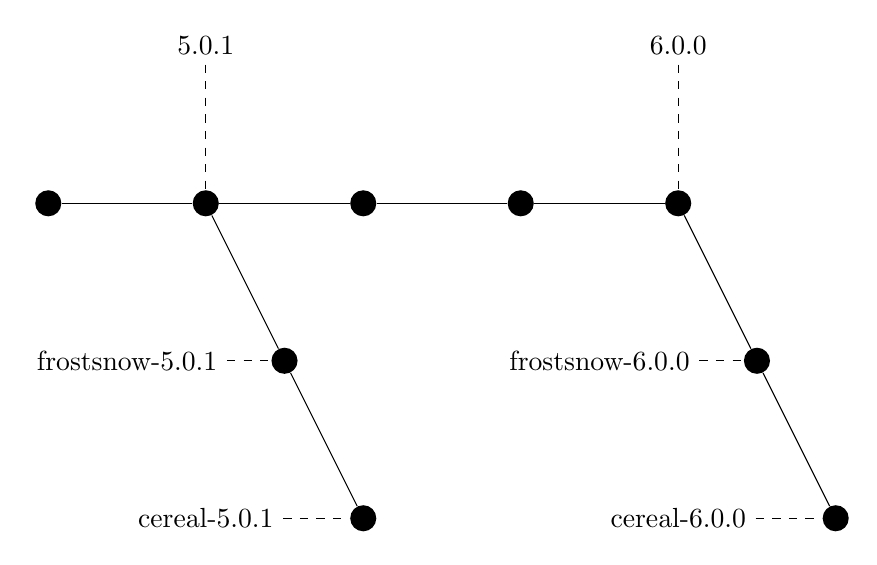
\begin{tikzpicture}
	% Using absolute values instead of relative values is sloppy.
	\node(A) [fill,circle] at (0, 0) {};
	\node(B) [fill,circle] at (2, 0) {};
	\node(C) [fill,circle] at (4, 0) {};
	\node(D) [fill,circle] at (6, 0) {};
	\node(E) [fill,circle] at (8, 0) {};
	\node(B1) [fill,circle] at (3, -2) {};
	\node(B2) [fill,circle] at (4, -4) {};
	\node(E1) [fill,circle] at (9, -2) {};
	\node(E2) [fill,circle] at (10, -4) {};
	\draw (A) -- (B);
	\draw (B) -- (C);
	\draw (C) -- (D);
	\draw (D) -- (E);
	\draw (B) -- (B1);
	\draw (B1) -- (B2);
	\draw (E) -- (E1);
	\draw (E1) -- (E2);
	\node (game5) at (2, 2) {5.0.1};
	\node (frostsnow5) at (1, -2) {frostsnow-5.0.1};
	\node (cereal5) at (2, -4) {cereal-5.0.1};
	\draw[dashed] (game5) -- (B);
	\draw[dashed] (frostsnow5) -- (B1);
	\draw[dashed] (cereal5) -- (B2);
	\node (game6) at (8, 2) {6.0.0};
	\node (frostsnow6) at (7, -2) {frostsnow-6.0.0};
	\node (cereal6) at (8, -4) {cereal-6.0.0};
	\draw[dashed] (game6) -- (E);
	\draw[dashed] (frostsnow6) -- (E1);
	\draw[dashed] (cereal6) -- (E2);
\end{tikzpicture}
}
\end{makeimage}
\caption{Simplified layout of the Minetest game \texttt{git} repo using hypothetical \texttt{6.0.0} game version.  Note that, because of the way ebuilds specify commits, each version would require a separate branch with this method.}
\end{figure}
\end{center}

In this case, even if I rebased my patches on the new game version without removing the old patches, I'd have to create a separate branch for each game type and version, whose name is the type and version of the game without the sub-minor version; this is in addition to a tag for each type and sub-minor version, resulting in cumbersome branch \& tag specifications that pollute the branch namespace.  This is what I initially did, but, now that I've had time to reflect and write this blog, I think it'll be far more sane to just \emph{do an actual merge} into the respective game type's branch; that will allow me to keep the history intact and the branch specification sane.  Thus, this was a great example of over-thinking as a result of using a process which doesn't fit the problem.

With the games now in an easily-installable state thanks to the repos and ebuilds, it was time to tackle my authorization problem.

\subsubsection{Preventing Unauthorized Access}
Some admins leave their servers open to the public as a service to the community; kudos to those people.  While I enjoy having such services around, I was not willing to put the time and effort into moderating and maintaining such a service, and so what I needed was some kind of authorization system.  By default, Minetest allows users to arbitrarily create new accounts, so I needed some way to inhibit that.

What form the authorization solution would take wasn't known to me at the beginning, hence I prepared to buckle in for the long haul.  I began by checking out the \htmladdnormallink{Minetest Wiki server hosting page}{https://wiki.minetest.net/Setting_up_a_server}, but didn't find anything relevant to my needs.  Checking the \texttt{minetest.conf} example in \verb|/usr/share/doc/minetest-${VER}| showed a \texttt{default_password} field which meant users would have to know the password in order to create an account; while that would help somewhat, people might give the password to a friend, who would then give it to a friend, who would give it to a friend, \&c., and before I'd know it some really strange people would be joining.  No, that wouldn't work for me.  Next, I checked the \texttt{lua_api.txt} file in the aforementioned documentation folder, and found in there a section on authentication!  Perhaps, in true Minetest style, what I needed would be in a mod, so I began to search the \htmladdnormallink{Mod Releases}{https://forum.minetest.net/viewforum.php?f=11\&sid=2e1dbb2169d33b1d6d2da944c86c89b9} subforum, where I found the \htmladdnormallink{auth_rx}{https://forum.minetest.net/viewtopic.php?f=9&t=20393&hilit=auth_redux} mod.  After reading the forums post and documentation, I determined that this mod would likely suit my needs and began to try it out.

Turned out that \texttt{auth_rx} mod used a custom authentication database format.  In order to \htmladdnormallink{migrate}{https://github.com/sorcerykid/auth_rx/wiki/Basic-Database-Import}, a tool called \texttt{convert.awk} was provided in \texttt{auth_rx/tools}; the tool worked by reading the plaintext \texttt{auth.txt} file and converting it to the mod's alternate \texttt{auth.db} file.  You may recall that I had previously migrated from plaintext to SQLite3; well, as far as I could tell, the tool only worked on the plaintext format, so I had to re-migrate from SQLite3 back to normal plaintext, then migrate to the mod's format.  I also ran the \htmladdnormallink{advanced import}{https://github.com/sorcerykid/auth_rx/wiki/Advanced-Database-Import} in order to collect some metadata, though the data was somewhat tainted due to the fact that the import did not appear to take into account that multiple worlds (mostly test ones) had all been logged to the same file.  With the authentication data in place, I had to write some login rules.

The \texttt{auth_rx} mod used a Domain-Specific Language (DSL) known as the \htmladdnormallink{Minetest Authentication Ruleset Schema}{https://github.com/sorcerykid/auth_rx/wiki/Working-with-Rulesets} (MARS).  In addition to specifying the conditions that would allow or prevent users from logging in, the rulesets also allowed specifying custom error messages when access was denied.  Luckily for me, the very first example showed how to prevent users from creating new accounts!  Combining that with the custom error message, I was able to both block new, unauthorized users and to provide a message telling them how they could contact me in order to get an account created.  There was one caveat, though: how was I supposed to create an account now?  In-game, there are commands to remove an account, but must have been assumed that users would just create accounts by logging in, so there was no corresponding command to create an account.  For now, I used the power of MARS in order to implement a quick hack: logins from my IP address would be allowed to create an account.  Sure, it's not secure against someone who can spoof my IP address, but, dear reader, please promise not to tell those people until I implement a proper solution.  One last enhancement I made was, again following the examples in the documentation, to rate-limit logins after consecutive failures, much like \texttt{fail2ban};  I set a \texttt{fail all} rule to check for \texttt{\$ip_attempts gt 0}, \texttt{\$ip_failures gte 7}, and \texttt{age(\$ip_newcheck) lt 5m} to throttle players for 5 minutes after 7 failed login attempts.  The full configuration file, with my IP and e-mail redacted, was thus:

\begin{quote}
\begin{verbatim}
# Disable new player joins.
try "You must have an account created in order to join this server.  If you would like an account created, please e-mail the server admin at 'redacted@redactions.org' with your desired account name and, optionally, your desired password."
fail all
# FIXME: Implement non-hacky way to allow new player creation.
unless $addr eq 1.2.3.fake
if $is_new eq $true
continue

# Ban after frequent failures.
try "Too many consecutive login failures, please wait 5 minutes before trying to log in again"
fail all
if $ip_attempts gt 0
if $ip_failures gte 7
if age($ip_newcheck) lt 5m
continue

# Allow player login attempt.
pass now
\end{verbatim}
\end{quote}

\begin{figure}
\begin{center}
\includegraphics[scale=0.5]{files/blog/2019_07_20_minetest_5_0_1_upgrade_and_server_hosting/2019_07_20_access_denied.png}
\caption{New users must have an account created for them.}
\end{center}
\end{figure}

Though I now had what I wanted for logins, all was not yet well, as, whenever I logged into the server, I always had the \texttt{creative} privilege, giving me unlimited resources and mining power, though other users did not.  This was bad because I wanted to be able to actually play the game as a regular user, but still have admin privileges in case they were needed.  Revoking the offending privilege via the \verb|/revoke ${NAME} creative| did not work; I also tried manually editing the authorization files, but nothing seemed to work.  Perhaps I'd gotten the server into a broken state with all of my trials?  I tried wiping it and re-migrating, but still had the same issue.  What did work, though, was to remove the \texttt{auth_rx} mod, but that was hardly an acceptable solution, so I decided to dig into the mod's code in order to see if I could fix the issue.  Searching for the authentication APIs mentioned in Minetest's \texttt{lua_api.txt} documentation file quickly led me to some code with the telling comments "\texttt{grant server operator all privileges}", "\texttt{(TODO: implement as function that honors give_to_admin flag)}", and "\texttt{server operator's privileges are immutable}"; it turned out that the code determined who the admin was from the \texttt{name} variable in \texttt{minetest.conf} and then gave them all privileges immutably, not even storing them in the authorization file.  While the comments suggested that there's a proper solution using a \texttt{give_to_admin} flag, I wasn't keen on trying to figure it out at this point time, so I simply made a fork with the offending code \htmladnormallink{removed}{https://github.com/clinew/auth_rx/commit/583daec42043141eacd0860e3115b6c10d7cab80}.  This meant that I had to grant myself all privileges before adding the modified version of the mod, otherwise I wouldn't be able to get them back, but that was a simple one-time setup.  It wasn't the most elegant solution, but it was good enough for now.

With the authentication mod figured out, I at last added it to my games.  At this point, even though I didn't have all of my required features, I had the ones that would allow me to feel comfortable hosting a live server while I worked on the other needed features, so it was time to prepare the server.

\subsubsection{Preparing the Server}
This is the sort of boring but nuanced work that makes life a bit more tedious than one might like.  I'm not going to cover generic server set-up (SSH, \texttt{fail2ban}, \texttt{logrotate}, \&c.) besides noting that DNS did not seem to like having two separate A records (\texttt{minetest.frostsnow.net} and \texttt{mt.frostsnow.net}) pointing to the same IP address, so I used a CNAME record for one of them instead.  After doing generic server set-up, within the Minetest world itself I had to make a couple of changes, such as setting the \texttt{gameid} variable in \texttt{world.mt} to point to my \texttt{mt_cereal} game, giving myself an actual password by logging in and running \texttt{/setpassword}, and setting my privileges and migrating the authentication database as described in the previous section (I was actually using a temporary, test instance earlier).  Lastly, I decided to set a static spawn point away from all the stuff that I'd already built; this was done by setting \texttt{static_spawnpoint} in \texttt{minetest.conf}, but, as the setting applies to all worlds created using that configuration file, and not just my current world, that meant that, in the future, I'd have to make sure any additional worlds can either use that spawnpoint or install said worlds into a different location.  I then built a small house with some basic server rules and a craftguide at the spawnpoint.

\begin{figure}
\begin{center}
\includegraphics[scale=0.25]{files/blog/2019_07_20_minetest_5_0_1_upgrade_and_server_hosting/2019_07_20_starting_hut.png}
\caption{New users spawn on the stone block in the center of the hut, where they can read the server rules on the left, rest in the bed in the corner, or view the craftguide sign on the right.}
\end{center}
\end{figure}

Actually, things didn't go quite this straightforwardly, as I encountered the following error when trying to install Minetest: \verb|/var/tmp/portage/games-action/minetest-5.0.1-r1/work/minetest-5.0.1/src/irrlichttypes.h:33:10: fatal error: irrTypes.h: No such file or directory|.  Looking into the matter, it appeared that \htmladdnormallink{Irrlicht}{https://en.wikipedia.org/wiki/Irrlicht_Engine} was the game engine upon which Minetest was built, and the unstable ebuild I was using did not require it when the \texttt{dedicated} USE flag was specified.  Now, I could have tried to fix this properly, but, again, please forgive me, I simply installed \texttt{dev-games/irrlicht} manually (in fact, it appears that newer revisions of the ebuild have done away with the flag entirely).  Once Minetest was installed I configured it to use my world by editing the \texttt{ARGS} parameter in \texttt{/etc/conf.d/minetest-server} to include \verb|--world /var/lib/minetest/.minetest/worlds/cereal|, and also added \verb|--logfile /var/log/minetest/minetest-server.log|, since the default location under \texttt{/var/lib} for log files is blasphemous in my eyes.  A couple weeks later, when the ebuild was updated (as previously hinted), I also needed to change the \texttt{MINETESTBIN} variable from \texttt{/usr/bin/minetestserver} to \texttt{/usr/bin/minetest} and add \verb|--server| to \texttt{ARGS}.  It appeared that the ebuild was marked as unstable for a reason!

Now the server was installed, configured, and running.  I'd gotten far, but there were still a number of features that I wanted to add before I would consider things to be good enough for now.

\subsubsection{Building the IRC Bridge}
One feature that I considered an absolute must was to link my Minetest server with my IRC server.  This would make it easier both to socialize with my friends and to monitor the server for any suspicious activity.  Thankfully, a mod for this \htmladdnormallink{already existed}{https://github.com/minetest-mods/irc}.  Since the mod didn't come with my distribution, I had to manually install its \texttt{luasocket} dependency, found at \texttt{dev-lua/luasocket}.  Then I added the mod to my custom games as yet another submodule, and configured my world to trust it via setting \texttt{secure.trusted_mods} to include \texttt{irc} in \texttt{minetest.conf}.

Though I had the mod installed, connecting to my server is not straightforward, as I both require the use of TLS and a properly-signed \emph{client} certificate.  From the mod's documentation it did not appear that the mod supported specifying a client key and certificate, but that was okay, because I could use \texttt{stunnel} as a workaround.  I've written about using \texttt{stunnel} in a \htmlref{previous blog post}{2017-08-23-securely-syncing-the-gentoo-repository-via-a-local-server}, and so won't cover the basics again here, but, of course, it seems impossible to touch TLS without getting burned somehow, and this experience was no exception.  Instead of connecting like it should have, I kept getting the following error in my Minetest log: \verb|ERROR[Server]: IRC: Connection error: 127.0.0.1: /usr/share/minetest/games/test/mods/irc/irc/init.lua:138: closed -- Reconnecting in 600 seconds...|.  I couldn't figure out what was wrong with the connection, so I set \texttt{debug = 7} in \texttt{stunnel.conf}, tried reconnecting, and then opened up \texttt{stunnel.log}, which showed: \verb|LOG3[1]: SSL_connect: 14077410: error:14077410:SSL routines:SSL23_GET_SERVER_HELLO:sslv3 alert handshake failure|.  Well, that still didn't help, so I checked \texttt{ircd.log} on my IRC server and saw: \verb|OpenSSL handshake error 'error:1408A0C1:SSL routines:ssl3_get_client_hello:no shared cipher' for '1.2.3.fake' port '6697'|.  "\texttt{no shared cipher}"?  I had nothing set explicitly in \texttt{stunnel.conf}, but checking \texttt{stunnel.log} showed \texttt{Ciphers: HIGH:!aNULL:!SSLv2:!DH:!kDHEPSK} and InspIRCd was configured to use \texttt{DHE-RSA-AES256-GCM-SHA384}.  I tried setting \texttt{ciphers = ALL} in \texttt{stunnel.conf}, which then connected successfully using\ldots "\texttt{TLSv1.2 ciphersuite: DHE-RSA-AES256-GCM-SHA384 (256-bit encryption)}".  Seriously?  I was hardly in the mood to truly deal with this weirdness, so I configured both \texttt{stunnel} and InspIRCd to use \texttt{HIGH:@STRENGTH} as their cipher list, which actually worked as expected.  Maybe one day I'll take another look at this, and what exactly TLS considers "\texttt{HIGH}"-strength ciphers.

As if dealing with perplexing cipher-negotiation errors wasn't enough, I also ran into a permissions issue which required a patch.  Rather than have the client certificate and key be readable by all users, I wanted to harden my setup a little by making it only readable by the user which the server is run as; in addition, rather than run \texttt{stunnel} as root, I wanted it to also run as the aforementioned user.  Running it as a different user was easily done by setting \texttt{setuid} and \texttt{setgid} in \texttt{stunnel.conf}, but after I did this, \texttt{stunnel} no longer started!  Reading \texttt{stunnel.log} this time showed \texttt{Cannot create pid file /run/stunnel/stunnel.pid} and \texttt{create: Permission denied (13)}.  Checking permissions on the \texttt{/run/stunnel} directory showed that it was owned by \texttt{stunnel:stunnel} and, logically enough, did not have write access for other.  Easy enough fix, right?  I ran \texttt{chown} on it in order to fix the permissions, re-launched \texttt{stunnel}, and it died again!  Why?  Same reason!  Looking at the directory again showed that its permissions had been reverted!  After some digging I found in \texttt{/etc/init.d/stunnel} the line \verb|checkpath -d -m 0755 -o stunnel:stunnel -q $(dirname ${PIDFILE})|; turns out that the daemon initialization script was helpfully correcting permissions on that directory but did not take into account that the owner and group might not be the default.  The solution was easy enough: in the initialization script, grab the values of \texttt{setuid} and \texttt{setgid} from \texttt{stunnel.conf} in the same manner that the init script's \texttt{PIDFILE} value was grabbed, then use those values for the permissions of the directory; I filed a \htmladdnormallink{bug \& patch}{https://bugs.gentoo.org/show_bug.cgi?id=687046} for the issue, but, at the time of this writing, have yet to hear back.  Well, I got it working on my system, so good enough for now.

After I'd established my TLS tunnel it was time to focus on configuring the bridge just the way I wanted it.  Like the static spawnpoint mentioned in the previous section, these settings went into \texttt{minetest.conf} and so would apply to any world created under that configuration.  Obvious enough was pointing \texttt{irc.server} to the address of the TLS tunnel (otherwise I wouldn't have been able to test it, obviously), but less conspicuous was \texttt{irc.port}, which was strangely absent from the \texttt{README} but useable nonetheless.  Next, I set the bridge's IRC nickname with \texttt{irc.nick}, joined channel with \texttt{irc.channel}, and made sure to register both the nick and the channel on the server.  By default, Minetest players are able to disconnect from the bridge with \texttt{/part}, but, as part of the reason for the bridge is to monitor the Minetest server, I disabled this by setting \texttt{irc.enable_player_part} to \texttt{false}; I also set \texttt{irc.send_kicks} to \texttt{true} so that any kick messages would be sent to the IRC channel.  An interesting feature of the bridge is that it allows users to opt out of bridging their communication by prefixing their message with \verb|[off]|; I wanted this feature for the IRC channel, but not for the Minetest server.  I couldn't find an existing option for this in the mod, so I created a \htmladdnormallink{fork}{https://github.com/clinew/irc/tree/5cf3e47db7f295b0dae85cf1b1abddf8aee57602} with the change, and incorporated that fork into my games instead.

\begin{figure}
\begin{center}
\includegraphics{files/blog/2019_07_20_minetest_5_0_1_upgrade_and_server_hosting/2019_07_20_irc_bridge.png}
\caption{The IRC bridge in action on both the Minetest server (above) and IRC server (below).}
\end{center}
\end{figure}

There was one, in my opinion, sub-optimal thing about this solution overall: the tunnel was currently bound to the loopback interface, which meant that, in the case of multiple servers, I'd have to take care to avoid having multiple tunnels bind to the same port, and, theoretically, malicious programs running on the node could connect to the server.  What might work instead for the Minetest side of the tunnel would be to bind to a UNIX domain socket rather than the loopback interface; \texttt{stunnel} appears to support this, but the Minetest IRC mod does not appear to.  Perhaps it would make a good addition someday, but, for now, I wanted to move onto the next task.

\subsubsection{Recovering from Crashes}
One of the mods I use has this bug which, once in a great while, causes the server to crash.  I'm not sure what exactly causes the bug, but it's rare, and the server is just fine after a restart.  This isn't a big deal when I'm playing on my own as I can simply restart the server, but I'd rather it not happen to another player when I'm gone and unable to restart it.  Gentoo had a solution to this, but it would have been rather tacky, in my opinion, to test how well a production server handled crashes by, well, crashing it.  Instead, what I needed was a test server.

Rather than configuring a test server all by hand, I decided to follow-through on my package-manager as configuration-management plans.  I began by creating a \htmladdnormallink{\texttt{games-action/mt_test}}{https://github.com/clinew/overlay_frostsnow/tree/master/games-action/mt_test} ebuild, and had it create a custom user for the test server by invoking \texttt{enewgroup} and \texttt{enewuser} in \texttt{pkg_setup()}.  Some weirdness followed, as Portage expected a directory by the package name to be created, so I ran \verb|mkdir ${WORKDIR}/${P}| in \texttt{src_unpack()} in order to hackishly create it.  Then I copied the daemon's configuration file, \texttt{minetestserver.confd}, from the regular Minetest ebuild, but it needed a few modifications; I changed \texttt{USER} to be modifiable, gave \texttt{PIDFILE} a world-specific suffix, and changed the \texttt{ARGS} logfile argument to both point to \texttt{/var/log} rather than \texttt{/var/lib} and to contain a world-specific suffix for its log directory.  I then had the ebuild set these values via \texttt{sed} as part of \texttt{src_prepare()}.  One of the default Gentoo services, \texttt{net}, allowed one to create specific network interfaces by creating symbolic links to its initialization script in \texttt{/etc/init.d} (for example, creating the symbolic link from \texttt{net.eth0} to \texttt{net} would create the \texttt{eth0} interface); mimicking this idea, I had the ebuild create the service \texttt{minetest-server.test} by creating a symbolic link to \texttt{minetest-server} in the \texttt{src_install()} function and then installed my custom \texttt{.confd} with the same service name in \texttt{/etc/conf.d}.  The logging directory was created via running \verb|keepdir /var/log/minetest-${WORLD}| in the same \texttt{src_install()} function.  This created a skeleton configuration for the game.

Now, Portage doesn't have anything that I know of that'd be like Chef's data bags for hosting the actual world data, but one could probably emulate that using some kind of hosting service.  I didn't want to do that, however, so the actual game data I copied manually from the production world.  Surprisingly enough, after changing the \texttt{port} variable in \texttt{minetest.conf} things seemed to work pretty well, though I quickly changed \texttt{irc.nick} and \texttt{irc.channel} as well in order to prevent the name collision and main channel spam.  The ebuild created for the job can be found \htmladdnormallink{here}{https://github.com/clinew/overlay_frostsnow/commit/3b03ab69f524872c86272c1ca4090106cbd0925c}.  Satisfied with my test server setup, it was time to actually configure auto-restart.

By default, Portage would use the \texttt{start-stop-daemon} in order to control services, but there was another option, the \texttt{supervise-daemon}, which would monitor and restart crashed services; this could be configured by the service's initialization file in \texttt{/etc/init.d} as documented in \texttt{openrc-run(8)}.  The default Minetest server had defined custom \texttt{start()} and \texttt{stop()} functions for the actions of the same name.  I removed the symlink which I had created earlier, replacing it with a copy of the file it was previously pointing to, and then tried to modify these functions in order to suit my needs, but kept getting weird results, such as the service respawning forever, even after I had told it to actually stop.  Eventually, I tried removing these custom functions (leaving the service to run its default ones) and instead only defining the relevant variables based on their values in the \texttt{/etc/conf.d} file, and it worked!  The resulting file can be found \htmladdnormallink{here}{https://github.com/clinew/overlay_frostsnow/blob/d973f9911766ad2d01704757d13eb27a5e2ab30c/games-action/mt_test/files/minetestserver.initd}; the main trick was to set the \texttt{supervisor} variable to \texttt{supervise-daemon} so it'd monitor and restart the service.  After that, I could crash the service (via \texttt{kill}, or it could crash on its own) and it'd restart automatically.  Once I'd ported the changes over to the production server, I had one final task left.

\subsubsection{Creating a Backup Solution}
There was no way I was going to go through all of this hosting effort and not have some kind of backup solution, but settling on a particular method was tricky.  I wasn't keen to store all of my data in the cloud where I may be cut off from it, but that meant I'd somehow need to retrieve it from the Minetest server onto my home server, thus making the solution more complex.  I also didn't want to use large amounts of data storing backups, nor set up a particularly complex data delta and deduplication scheme right then, so what I ended coming up with were some handwritten scripts to create, retrieve, and cycle the backups.  In addition, I tried to make my life easier in the long run by using Portage to install and configure the scripts by creating ebuilds for them.  I began by working on the Minetest server side.

Generating the backup itself was simple enough.  There was some discussion on the forums regarding whether one could safely run backups without shutting the game down first, but without much consensus, so I decided to play it safe and shutdown the game server when creating any backups.  The steps were simple: clean any existing backup copy, shutdown the server, create the backup with \texttt{tar}, restart the server, then compress the backup with \texttt{bzip2}.  Since I would eventually like to be able to host multiple instances, I parameterized the script to accept the service name as the first argument and the Minetest user's home directory as the second, but the script would use a sane default if these were not specified.

With the backup-generating script created, it was time to install it, but, rather than manually install it, I decided to use an infrastructure-as-code approach and have an ebuild named \htmladdnormallink{app-backup/minetest-backup}{https://github.com/clinew/overlay_frostsnow/tree/master/app-backup/minetest-backup} do so for me!  As with the test server, I used \texttt{enewgroup} and \texttt{enewuser} within \texttt{src_unpack} in order to create a special user for the task, in this case named \texttt{mtbackup}.  Since I (currently) wanted the backup script to run daily with the default arguments, I could install it directly by placing the script into the \texttt{files} subdirectory of the ebuild, then running \texttt{exeinto /etc/cron.daily} followed by \verb|doexe ${FILESDIR}/mtbackup| in \texttt{src_install()}; this would run the backup (at 3:10 a.m.) as the root user rather than the \texttt{mtbackup} user, but I needed that level of permission in order to control the service anyways.  In addition to generating the backup, I would also need to pull it, preferably securely and with proper authorization, so I chose to use OpenSSH's \texttt{scp}; this meant I'd have to authorize the \texttt{mtbackup} user for login.  Now, Portage has a useful \htmladdnormallink{sandbox}{https://devmanual.gentoo.org/general-concepts/sandbox/} feature to prevent mis-behaving ebuilds from installing packages where they shouldn't, but I wasn't using Portage like I should have, so I had to disable the sandbox feature and face Portage's unhappy messages.  In the ebuild, I disabled the sandbox with \texttt{addwrite /home/mtbackup}, set the insertion directory with \texttt{insinto /home/mtbackup.ssh}, added the authorized keys file with \verb|doins -r ${FILESDIR}/authorized_keys|, and finally made \texttt{mtbackup} the owner of their configuration with \texttt{fowners -R mtbackup:mtbackup /home/mtbackup/.ssh}; the user's key was now authorized!  Lastly, as a courtesy, I added a \texttt{motd} entry to the \texttt{minetest.conf} file warning users of the daily downtime for backups.  Though I was now able to generate a nightly backup, I would still need to pull and store them.

Retrieving backups ended up being a bit trickier due to my space constraints and workaround; what I desired was to keep 7 daily backups, 5 weekly backups, and infinite monthly backups.  This would make space-usage manageable while still allowing a decent timeframe for catching any kind of errors or allowing world-restoration in the case of out-of-control vandalism.  In the hopes that I wouldn't have to roll my own script, I decided to see if I could trick \texttt{logrotate} into doing what I wanted for me.  At first things seemed to be going well, I could set rotation periods such as \texttt{daily}, \texttt{weekly}, and \texttt{monthly}, rotation count with \texttt{rotation #}, and timestamp the files with \texttt{dateext} and \texttt{dateformat}.  Unfortunately, each of these rules expected a target, and subsequent definitions overrode previous ones, so pointing multiple rules at the same file wouldn't work; I could have made multiple hard links to the same file contents and pointed a rule to each of them, but it would have gotten ugly and cluttered quickly.  In addition, I had to specify an alternate state file for keeping track of rotations, couldn't figure out a way to keep an infinite number of rotations (for the monthly backups), and found testing to be rather difficult.  I abandoned the idea and wrote a script instead.

The script itself is pretty average: there's a \texttt{rotate} function for its namesake, I use hard links for the backups so as not to duplicate data, and allow \texttt{SOURCE} and \texttt{DESTINATION} parameters as the first and second arguments to the script, respectively; I also had to add \texttt{-o BatchMode=yes} to \texttt{scp} in order to prevent the script from potentially stalling.  Now, creating the ebuild, \htmladdnormallink{app-backup/minetest-backup-client}{https://github.com/clinew/overlay_frostsnow/tree/master/app-backup/minetest-backup-client}, was way more fun.  As before, I added a new user and group, this time called \texttt{mtbackupc}, then I added SSH configuration again, except this time I added the \texttt{known_hosts} file containing the Minetest server's public key rather than the \texttt{authorized_keys} file.  The backup script needed to be handled a bit differently this time, though, as I wasn't going to have it race with backup creation; I needed to run it at a later time.  I began by installing the script as a regular executable file in \texttt{/usr/bin} called \texttt{mtbackupc}, then, after some digging, found a way to manually insert a cron job for the \texttt{mtbackupc} user at \texttt{/var/spool/cron/crontabs/mtbackupc} as file contents \texttt{0 4 * * * mtbackupc} in order to have the script run daily at 4:00 a.m. (if the backups take over 50 minutes to complete on the Minetest server I'm totally hosed here); this was followed by a call to \texttt{fowners mtbackupc:crontab} in order to fix permissions on the file.  Last, I would have to manually install the key, as posting a private key publicly as part of the repo would be foolish, but, in case I ever forgot to install the key, I added a check in \texttt{pkg_postinst()} that would warn me during ebuild installation if no file was located at \texttt{/home/mtbackupc/.ssh/id_ed25519}.  With both pieces now in place, I now had a working backup solution.

Developing the backup solution raised an interesting question about how the backup ebuilds ought to be designed that I've yet to fully resolve in my head.  The question is one about how configuration-dependent the ebuilds ought to be; for example, installing a \texttt{known_hosts} file for a specific key, while convenient, is very much dependent on a particular key, in addition, the script itself currently uses a hardcoded \texttt{mt.frostsnow.net} domain.  It might be better practice to include all generic bits in one ebuild, then create another ebuild, perhaps under something like \texttt{sys-conf}, with all configuration-dependent stuff that would then require the previous ebuild (except made generic) as a dependency.  Similarly, should Minetest ebuilds like \texttt{games-action/mt_test} include a skeleton configuration for the server or pull in the actual data as well?  I'm currently leaning towards a skeleton configuration, so that others can reproduce the world if they wish to but my instance of it will be privately managed by myself.  The world is also too large to put directly in a repo.

One last note of amusement for me is that I actually developed the ebuilds on a test VM before deploying them to production, and, when I uninstalled their packages, Portage removed the files it had installed as well!  This was unlike Chef, where I would have needed to write a separate recipe that would undo the work of the previous one.  Though, Portage did leave the users, and, in fact, failed to clean the directory \texttt{/home/mtbackupc}, as I had actually logged into that user in order to do some debugging, thereby creating a \texttt{.bash_history} file and causing Portage to complain that the directory was not empty and would thus not be removed (but the files which had been installed there by the ebuild were removed).  Pretty neat, though not entirely relevant to my needs and with arguable robustness.

\subsection{Future Work}
As answers often beget more questions, so, too, did this work beget more work.  First, I needed a sane way to create a new user account as admin, probably from an in-game command, though it would also be useful if I had a bash command to do so.  Second, I'd like a proper fix for the privilege issue in \texttt{auth_rx} that would allow me to arbitrarily add and revoke privileges on my admin account.  Thirdly, as a nice-to-have, have the \texttt{auth_rx} mod properly detect new servers, as right now it fails on new servers because there's no player database to initialize from, but there also isn't one to import!  Fourth, getting the \texttt{irc} mod to connect to UNIX domain sockets would allow me to easily set up new server IRC bridges via \texttt{stunnel} without worrying about port collisions and providing a layer of access control (I think).  Fifth, I'd like to create a proper \texttt{mt_cereal} ebuild in the same way I have \texttt{mt_test}.  Finally, it might be useful to pipe the Minetest log file to a locked IRC channel so I can monitor the game from IRC, but that may actually be a bit too much.

\begin{figure}
\begin{center}
\includegraphics[scale=0.25]{files/blog/2019_07_20_minetest_5_0_1_upgrade_and_server_hosting/2019_07_20_hosted.png}
\caption{Screenshot of the now properly-hosted game world.}
\end{center}
\end{figure}

That will all have to wait for now, though.  Things appear to be running smoothly, and hopefully all of the work I put into configuration management will pay off in the long run (it certainly made installing the test server a bit easier).  My current goal is to keep things running smoothly while I take a break to work on other things, and then get back to this in due course.

\subsection{Addendum 2019-07-21}
Shortly after posting this blog, my friend ushered me back to my main base, saying that he had a gift for me!  After a bit of nagging, I walked back to my base and saw:

\begin{figure}
\begin{center}
\includegraphics[scale=0.25]{files/blog/2019_07_20_minetest_5_0_1_upgrade_and_server_hosting/2019_07_20_crystal_maiden.png}
\caption{Crystal Maiden attentively watches over my base.}
\end{center}
\end{figure}

He'd created a pixel art version of \htmladdnormallink{DotA2's}{http://www.dota2.com} \htmladdnormallink{Crystal Maiden}{https://dota2.gamepedia.com/Crystal_Maiden} as decoration for my base!  Super cool, and a nice gift to receive after having finished the blog!


% Adding the InspIRCd v3 ebuild
\section{2019-05-27 Adding the InspIRCd v3 ebuild}
Version 3 of InspIRCd has many changes, and, as proxy-maintainer, I have the responsibility of updating the ebuild.  In order to do this, I began by getting the old ebuild to work without \texttt{USE} flag modifications, then I began updating the \texttt{USE} flags, and finally I tweaked configuration file installation and sent a PR upstream.

\subsection{Getting the ebuild working}
Earlier, I'd created a v3 ebuild in order to test some features of mine, but it was a hack-job; I merely got the program to install without actually worrying about all the features offered and whether they'd changed.  Nonetheless, getting the program to install is always a good start, so this is how I began.  The first issue I ran into was expected: there is a patch to the program (InspIRCd uses a custom build process, not autotools) that updates paths in the configuration and build files to what Gentoo expects, and this patch had broken on the newer version of the tool.  This isn't a particularly difficult fix, but if you're a git baby like me and don't really have a method for generating diffs outside of version control this process can be rather awkward as it isn't really feasible to just edit the patch file itself, and the source code that the patch is generated from isn't a part of the repository with the patch!  Luckily I had a cloned git repo of InspIRCd, so I attempted to apply the patch and fix it, but it turns out that simply running \texttt{git apply} will abort if the patch fails and not modify the working tree; instead I had to add the \texttt{--rej} option, giving:

\begin{quote}
\begin{verbatim}
	git apply --rej /path/to/ebuild/files/inspircd-2.0.27-fix-path-builds.patch
\end{verbatim}
\end{quote}

Then I was able to see what had applied with \texttt{git diff}, and then update what hadn't applied by opening up both the original and \texttt{.rej} files and editing the original based on what the \texttt{.rej} file was trying to do.  Once I had incorporated all of the changes from the \texttt{.rej} file, I could generate a patch with:

\begin{quote}
\begin{verbatim}
	git diff > /path/to/ebuild/files/inspircd-3.0.1-fix-path-builds.patch
\end{verbatim}
\end{quote}

Once the patch was in-place, the ebuild was successfully compiled and merged (in Gentoo terminology, after \emph{compilation} and \emph{installation}, a package is \emph{merged} into the live system), but the service wouldn't actually start!  After some digging I figured out that the v3 build process was setting the permission bits to \texttt{0750} for the main program and \texttt{0640} for the modules; this caused problems because the program was installed as \texttt{root} but the service tried to run the program as the \texttt{inspircd} user.  Looking at the configuration script showed me that I could supply \texttt{--uid} and \texttt{--gid} options, so I added them to the \texttt{src_configure()} stage and it built and ran successfully, but then I started to have second thoughts: the other programs under \texttt{/usr/bin} are all run as \texttt{root}, and would I really want a rogue InspIRCd process to be able to modify its binary?  No, I would have to find a different solution.  Thus I decided to manually set the permission bits in the \texttt{src_install()} phase with the code:

\begin{quote}
\begin{verbatim}
	fperms 0755 /usr/bin/inspircd{,-genssl}
	fperms -R 0755 "/usr/lib64/inspircd/modules/."
\end{verbatim}
\end{quote}

Note the ebuild-specific \texttt{fperms} in place of \texttt{chmod}; the latter modifies the image by treating the path as relative to the image directory and not the root filesystem.  After this, the program launched successfully, but there was a couple of minor things that I noticed during compile time.  First, \verb|--with-cc| was an unknown option, so I instead set the environment variable \texttt{CXX} when executing the configuration file.  Also, \verb|--enable-openssl| was reported as an unknown option; turns out it had been made into a module.  Once I'd cleaned these flags up, it was time to take a serious look at the compilation options, with an emphasis on the modules.

\subsection{Updating \texttt{USE} features of the ebuild}
The quintessential question I had when updating this ebuild was, "What modules changes will affect the ebuild?".  I began by reviewing the \htmladdnormallink{change log}{https://docs.inspircd.org/3/change-log}, but its focus was on runtime configuration, whereas mine was compile-time configuration.  Next I tried running \verb|configure --help| and from there \verb|configure --list-extras|; this gave me a list of modules which I then compared to the existing \texttt{USE} flags.  From this information I then built up the following list of flags and modules:

\begin{quote}
\begin{verbatim}
	Existing:
        - debug
        - geoip -> maxminddb (m_geo_maxmind)
        - gnutls (m_ssl_gnutls)
        - ldap (m_ldap)
        - mysql (m_mysql)
        - pcre (m_regex_pcre)
        - posix (m_regex_posix)
        - postgres (m_pgsql)
        - sqlite (m_sqlite3)
        - ssl (m_ssl_openssl)
        - tre (m_regex_tre)

        New:
        - re2 (m_regex_re2)
        - stdlib (m_regex_stdlib)
        - mbedtls (m_ssl_mbedtls)
        - sslrehashsignal (m_sslrehashsignal)

        Removed:
        - ipv6
\end{verbatim}
\end{quote}

Now that I had the list, the next question was how to test the flags.  Doing a test of each possible permutation of \texttt{USE} flags would result in an exponential number of tests, so I instead decided to try 1) compilation with no \texttt{USE} flags, 2) configuration with each \texttt{USE} flag individually, and 3) compilation with all \texttt{USE} flags.  Note that when testing each \texttt{USE} flag individually I opted to only test configuration and not compilation; this is because a full compilation for each flag would have taken very long, I'm mostly checking whether the appropriate module is enabled, and compilation will be tested well enough when all \texttt{USE} flags are enabled.  I also decided to test the existing flags before adding the new ones.

Testing the ebuild via compilation was easy enough, I simply had to merge it, but testing only the configuration was a bit more tricky.  To begin with, I'd run \texttt{emerge} with the \texttt{-o} option in order to install the dependencies of the package, ensuring I had the dependencies correct.  After that I'd use the \texttt{ebuild} command in order to run a specific function of the ebuild, such as configuration.  Thus testing the configuration stage of an ebuild was done by running \texttt{ebuild /path/to/package.ebuild configure}, followed by \texttt{ebuild /path/to/package.ebuild clean} so that subsequent runs would work.  In the cases where the library I needed was already installed on my system, I was able verify that the ebuild was including the correct package with \texttt{equery b /file/to/check}; for example, in order to verify which ebuld \texttt{libssl.so} came from I ran \texttt{equery b /usr/lib/libssl.so}, which then returned \texttt{dev-libs/openssl-1.0.2r (/usr/lib64/libssl.so.1.0.0)}.

Of course, things didn't quite go as smoothly as I'd hoped.  By default, the configuration stage of InspIRCd expects the user to be able to \emph{interactively} select which modules to enable and disable, but interactivity is not acceptable when running an ebuild; for this case InspIRCd allows the user to specify the \verb|--disable-interactive| argument, but there's a trick: modules must be configured in one invocation of the configure script, then a separate invocation of the script must be used to actually configure the project.  Easy enough, but, while the first invocation of the script configured the modules correctly, the second invocation would enable modules that hasn't been explicitly selected!  After digging in the code I found that, indeed, modules were automatically being enabled if their dependencies were found on the system.  After asking the developers about this one of them pointed to a \htmladdnormallink{patch}{https://github.com/inspircd/inspircd/commit/2cc524a1c6aa7af22e4c68232c5d6206c70ded4e} which added a \verb|--disable-auto-extras| option to disable module auto-selection.  I added the corresponding patch and argument to the ebuild, and things began working as expected.

Many of the modules were straightforward, but a couple involved a bit more digging.  The first was the \texttt{geoip} module, which existed in v2 of InspIRCd but not v3.  After a bit of searching, I found that \texttt{libgeoip} was considered obsolete and that its replacement was \texttt{libmaxminddb}.  Both appear to do some kind of geography lookup based on the user's IP address; the library defines the protocol for accessing the data, but the actual data has both a free and a licensed version.  It sounded like a whole pile of fun that I didn't want to get involved in, so I simply renamed the \texttt{USE} flag from \texttt{geoip} to \texttt{maxminddb} and changed the dependency from \texttt{dev-libs/geoip} to \texttt{dev-libs/libmaxminddb}.

Rather baffling was the \texttt{m_regex_stdlib.so} module.  It turns out that this module uses the regex library that comes with the C++11 standard, but that its support was noted in the configuration file as not compliant in GCC.  After some searching I found this \htmladdnormallink{post}{https://stackoverflow.com/questions/12530406/is-gcc-4-8-or-earlier-buggy-about-regular-expressions} which I interpreted to mean that the module would work correctly on all GCC versions >= 4.9, as well as a \htmladdnormallink{compatibility matrix}{https://gcc.gnu.org/onlinedocs/libstdc++/manual/status.html#status.iso.2011} which I found rather indecipherable; it wasn't apparent to me whether just the headers were built into GCC or if the implementation was also completed.  After some contemplation, I decided to go ahead and add \texttt{>=sys-devel/gcc-4.9.0} as a dependency to the ebuild.  I figured that perhaps I'd get a bug report in the future saying that a later version is required.

The rest of the module changes were simple.  The \texttt{m_ldap.so} module activation was simplified in InspIRCd's configuration from \texttt{m_ldapauth.cpp,m_ldapoper.cpp} to simply \texttt{m_ldap.cpp}.  The \texttt{m_regex_re2.so} module corresponded to a regular expression library, called "RE2", provided by Google; it required adding the \texttt{dev-libs/re2} package as a dependency.  The \texttt{m_ssl_mbedtls.so} module allowed yet another SSL library, previously called "Polar SSL"; it required adding the \texttt{net-libs/mbedtls} dependency.  The \texttt{m_sslrehashsignal.so} library didn't require any additional dependencies; it simply allowed rehashing the SSL configuration via the \texttt{SIGUSR1} signal, whereas, previously, a logged-in IRCop would have to issue the \texttt{/rehash -ssl} command.  There was no equivalent of the \verb|--enable-ipv6| options provided in v3, but, upon the asking the devs, I was told that this flag didn't actually do anything in v2 anyways; thus I removed the \texttt{ipv6} flag from v3.  Lastly came the \texttt{debug} \texttt{USE} flag; this flag was tricky because it corresponded to setting an environment variable \texttt{INSPIRCD_DEBUG} to a numeric value during compilation time, and the exact behaviour depended on the value specified.  I could have added a number of \texttt{debug} flags, but that would have been weird and bloated, so I decided against it, but the question then remained which value would be most sensible.  It turns out that the value \texttt{1} added \texttt{-Werror} to the compilation options and would thus cause compilation failures when, say, the compiler was upgraded, so it was \htmladdnormallink{not acceptable}{https://www.youtube.com/watch?v=Oqa9tKarkNA}.  The value \texttt{3} would remove all symbols from the binary and was meant explicitly for CI, so I ended up setting on the value \texttt{2}, which would include debug symbols but also enable optimizations.

Now that I'd added the \texttt{USE} flags, I also wanted to update their descriptions as \texttt{ebuild u inspircd} was showing some of the flags as \texttt{<unknown>}.  I opened up the Package Management Specification (PMS) documentation and found that I could add the flag to the \texttt{/usr/portage/profiles/use.desc} file for global use flags, and, supposedly, \texttt{/usr/portage/profiles/use.local.desc} for package-specific flags; I say "supposedly" because I was able to do so for the former, global, file but not the latter, package-specific file (the changes didn't appear to be getting picked up).  After asking for clarification in IRC, I was told to edit the \texttt{metadata.xml} file in the package's directory; this successfully updated the flags' descriptions for me.

Finally, I took a bit of time to ensure that the documentation files were being installed as expected.  InspIRCd is written such that the configuration files contain most of the needed documentation in them, but as a result the files are quite lengthy; they also include a couple tricks such as "die" statements which will terminate the program if not edited out, thus ensuring that the user actually bothered to configure their server properly rather than just running it blindly.  For this reason it wasn't clear to me whether the files should be installed into \texttt{/etc} or only placed in \texttt{/usr/share/doc}; installing them into \texttt{/etc} would cause the user to have to manually update their configuration files with \texttt{etc-update}, tediously removing the "die" statements and other cruft, but not doing so meant that the user's configuration would slowly diverge from the default, which could cause confusion later-on as options are removed, renamed, and added.  In the end I decided to merge the files into \texttt{/etc} as the user could easily enough forgo updating their files, but conscientious users could then more easily keep their configurations up to date.

\subsection{Merging to Mainline}
Merging went straightforward enough.  I created a \htmladdnormallink{pull request}{https://github.com/gentoo/gentoo/pull/12027} and got some pushback against the \texttt{stdlib} and \texttt{posix} flags as their names didn't make it clear what they did, and was also told that the GCC >= 4.9 dependency was pointless because simply having it installed wouldn't mean that it was being used due to Portage's slotting mechanism, and modern versions of Gentoo require at least 6.4 anyways.  So, I prefixed both of the flags with \texttt{regex-} and removed the GCC version dependency.  While I was doing this, though, my Internet went out for 6 says, during which a new version was released, thus, when my Internet was finally restored I also bumped the version to 3.1.0, which meant that I no longer had to include the patch adding \verb|--disable-auto-extras|, as it had been included in the upgrade.  A little later my pull request was merged!  I now await the bug reports\ldots


% Recompiling the Novena Linux Kernel Woes
\section{2019-05-07 Recompiling the Novena Linux Kernel Woes}
Normally\label{2019-05-07-novena-kernel-woes} when I have kernel problems they happen during a kernel upgrade, but not this time.  In fact, I'm not even sure \emph{when} the issues started happening.  Everything seemed fine at first, until one day when I tried to mount a USB storage device only to find that it wasn't working; instead, I got an error along the following lines (except not the \texttt{ipv6} module, obviously):

\begin{quote}
\begin{verbatim}
	[  622.972948] ipv6: no symbol version for module_layout
\end{verbatim}
\end{quote}

What could have caused this?  I'd done several major system upgrades since last time I recall modules working, but more suspect was the \texttt{CHOST} \htmladdnormallink{change}{https://www.gentoo.org/support/news-items/2018-09-07-arm-17-profile-migration.html}.  Well, it wasn't (and still isn't) clear to me exactly how much the \texttt{CHOST} change might affect the kernel, so the simplest solution would be to simply recompile the kernel, right?  That's when this happened:

\begin{quote}
\begin{verbatim}
	  CC      kernel/fork.o
	In file included from include/linux/kernel.h:11,
	                 from include/asm-generic/bug.h:13,
	                 from ./arch/arm/include/asm/bug.h:59,
	                 from include/linux/bug.h:4,
	                 from include/linux/mmdebug.h:4,
	                 from include/linux/gfp.h:4,
	                 from include/linux/slab.h:14,
	                 from kernel/fork.c:14:
	include/linux/log2.h:22:1: warning: ignoring attribute 'noreturn' because it  \
	conflicts with attribute 'const' [-Wattributes]
	 int ____ilog2_NaN(void);
	 ^~~
	In file included from kernel/fork.c:41:
	include/linux/syscalls.h:195:18: warning: 'sys_set_tid_address' alias between \
	functions of incompatible types 'long int(int *)' and 'long int(long int)'    \
	[-Wattribute-alias]
	  asmlinkage long sys##name(__MAP(x,__SC_DECL,__VA_ARGS__)) \
	                  ^~~
	include/linux/syscalls.h:191:2: note: in expansion of macro '__SYSCALL_DEFINEx'
	  __SYSCALL_DEFINEx(x, sname, __VA_ARGS__)
	  ^~~~~~~~~~~~~~~~~
	include/linux/syscalls.h:182:36: note: in expansion of macro 'SYSCALL_DEFINEx'
	 #define SYSCALL_DEFINE1(name, ...) SYSCALL_DEFINEx(1, _##name, __VA_ARGS__)
	                                    ^~~~~~~~~~~~~~~
	kernel/fork.c:1236:1: note: in expansion of macro 'SYSCALL_DEFINE1'
	 SYSCALL_DEFINE1(set_tid_address, int __user *, tidptr)
	 ^~~~~~~~~~~~~~~
	include/linux/syscalls.h:199:18: note: aliased declaration here
	  asmlinkage long SyS##name(__MAP(x,__SC_LONG,__VA_ARGS__)) \
	                  ^~~
	include/linux/syscalls.h:191:2: note: in expansion of macro '__SYSCALL_DEFINEx'
	  __SYSCALL_DEFINEx(x, sname, __VA_ARGS__)
	  ^~~~~~~~~~~~~~~~~
	include/linux/syscalls.h:182:36: note: in expansion of macro 'SYSCALL_DEFINEx'
	 #define SYSCALL_DEFINE1(name, ...) SYSCALL_DEFINEx(1, _##name, __VA_ARGS__)
	                                    ^~~~~~~~~~~~~~~
	kernel/fork.c:1236:1: note: in expansion of macro 'SYSCALL_DEFINE1'
	 SYSCALL_DEFINE1(set_tid_address, int __user *, tidptr)
	 ^~~~~~~~~~~~~~~
	include/linux/syscalls.h:195:18: warning: 'sys_unshare' alias between functions \
	of incompatible types 'long int(long unsigned int)' and 'long int(long int)' \
	[-Wattribute-alias]
	  asmlinkage long sys##name(__MAP(x,__SC_DECL,__VA_ARGS__)) \
	                  ^~~
	include/linux/syscalls.h:191:2: note: in expansion of macro '__SYSCALL_DEFINEx'
	  __SYSCALL_DEFINEx(x, sname, __VA_ARGS__)
	  ^~~~~~~~~~~~~~~~~
	include/linux/syscalls.h:182:36: note: in expansion of macro 'SYSCALL_DEFINEx'
	 #define SYSCALL_DEFINE1(name, ...) SYSCALL_DEFINEx(1, _##name, __VA_ARGS__)
	                                    ^~~~~~~~~~~~~~~
	kernel/fork.c:2000:1: note: in expansion of macro 'SYSCALL_DEFINE1'
	 SYSCALL_DEFINE1(unshare, unsigned long, unshare_flags)
	 ^~~~~~~~~~~~~~~
	include/linux/syscalls.h:199:18: note: aliased declaration here
	  asmlinkage long SyS##name(__MAP(x,__SC_LONG,__VA_ARGS__)) \
	                  ^~~
	include/linux/syscalls.h:191:2: note: in expansion of macro '__SYSCALL_DEFINEx'
	  __SYSCALL_DEFINEx(x, sname, __VA_ARGS__)
	  ^~~~~~~~~~~~~~~~~
	include/linux/syscalls.h:182:36: note: in expansion of macro 'SYSCALL_DEFINEx'
	 #define SYSCALL_DEFINE1(name, ...) SYSCALL_DEFINEx(1, _##name, __VA_ARGS__)
	                                    ^~~~~~~~~~~~~~~
	kernel/fork.c:2000:1: note: in expansion of macro 'SYSCALL_DEFINE1'
	 SYSCALL_DEFINE1(unshare, unsigned long, unshare_flags)
	 ^~~~~~~~~~~~~~~
	include/linux/syscalls.h:195:18: warning: 'sys_clone' alias between functions \
	of incompatible types 'long int(long unsigned int,  long unsigned int,  int *, \
	long unsigned int,  int *)' and 'long int(long int,  long int,  long int,  \
	long int,  long int)' [-Wattribute-alias]
	  asmlinkage long sys##name(__MAP(x,__SC_DECL,__VA_ARGS__)) \
	                  ^~~
	include/linux/syscalls.h:191:2: note: in expansion of macro '__SYSCALL_DEFINEx'
	  __SYSCALL_DEFINEx(x, sname, __VA_ARGS__)
	  ^~~~~~~~~~~~~~~~~
	include/linux/syscalls.h:186:36: note: in expansion of macro 'SYSCALL_DEFINEx'
	 #define SYSCALL_DEFINE5(name, ...) SYSCALL_DEFINEx(5, _##name, __VA_ARGS__)
	                                    ^~~~~~~~~~~~~~~
	kernel/fork.c:1849:1: note: in expansion of macro 'SYSCALL_DEFINE5'
	 SYSCALL_DEFINE5(clone, unsigned long, clone_flags, unsigned long, newsp,
	 ^~~~~~~~~~~~~~~
	include/linux/syscalls.h:199:18: note: aliased declaration here
	  asmlinkage long SyS##name(__MAP(x,__SC_LONG,__VA_ARGS__)) \
	                  ^~~
	include/linux/syscalls.h:191:2: note: in expansion of macro '__SYSCALL_DEFINEx'
	  __SYSCALL_DEFINEx(x, sname, __VA_ARGS__)
	  ^~~~~~~~~~~~~~~~~
	include/linux/syscalls.h:186:36: note: in expansion of macro 'SYSCALL_DEFINEx'
	 #define SYSCALL_DEFINE5(name, ...) SYSCALL_DEFINEx(5, _##name, __VA_ARGS__)
	                                    ^~~~~~~~~~~~~~~
	kernel/fork.c:1849:1: note: in expansion of macro 'SYSCALL_DEFINE5'
	 SYSCALL_DEFINE5(clone, unsigned long, clone_flags, unsigned long, newsp,
	 ^~~~~~~~~~~~~~~
	/tmp/ccxt2fNN.s: Assembler messages:
	/tmp/ccxt2fNN.s:5608: Error: .err encountered
	make[1]: *** [scripts/Makefile.build:290: kernel/fork.o] Error 1
	make: *** [Makefile:987: kernel] Error 2
\end{verbatim}
\end{quote}

"Oh, a system call error, this will be an easy fix", said no one, ever.  At this point I decided to run away screaming from the problem, but, after many months, I eventually got tired of not being able to use modules (or compile them into the kernel) and decided to buckle down and fix the problem.  As I suspected, it took a lot of guesswork.

\subsection{Troubleshooting}

I decided to begin by looking for low-hanging fruit.  Perhaps some simple configuration options, or a forgotten PEBKAC.  One hopeful candidate was to enable the \texttt{CONFIG_OABI_COMPAT} option, but it didn't help.  The next was to save the \texttt{.config} file, then re-emerge the kernel sources, you know, in case it had become\ldots~corrupted.  Or something.  That also failed to solve the problem.  The easy stuff was out, so it was time to look at the source.  The system call definitions in the file \texttt{include/linux/syscalls.h} showed:

\begin{quote}
\begin{verbatim}
	#define SYSCALL_DEFINE1(name, ...) SYSCALL_DEFINEx(1, _##name, __VA_ARGS__)
	#define SYSCALL_DEFINE2(name, ...) SYSCALL_DEFINEx(2, _##name, __VA_ARGS__)
	#define SYSCALL_DEFINE3(name, ...) SYSCALL_DEFINEx(3, _##name, __VA_ARGS__)
	#define SYSCALL_DEFINE4(name, ...) SYSCALL_DEFINEx(4, _##name, __VA_ARGS__)
	#define SYSCALL_DEFINE5(name, ...) SYSCALL_DEFINEx(5, _##name, __VA_ARGS__)
	#define SYSCALL_DEFINE6(name, ...) SYSCALL_DEFINEx(6, _##name, __VA_ARGS__)

	#define SYSCALL_DEFINEx(x, sname, ...)				\
		SYSCALL_METADATA(sname, x, __VA_ARGS__)			\
		__SYSCALL_DEFINEx(x, sname, __VA_ARGS__)

	#define __PROTECT(...) asmlinkage_protect(__VA_ARGS__)
	#define __SYSCALL_DEFINEx(x, name, ...)					\
		asmlinkage long sys##name(__MAP(x,__SC_DECL,__VA_ARGS__))	\
			__attribute__((alias(__stringify(SyS##name))));		\
		static inline long SYSC##name(__MAP(x,__SC_DECL,__VA_ARGS__));	\
		asmlinkage long SyS##name(__MAP(x,__SC_LONG,__VA_ARGS__));	\
		asmlinkage long SyS##name(__MAP(x,__SC_LONG,__VA_ARGS__))	\
		{								\
			long ret = SYSC##name(__MAP(x,__SC_CAST,__VA_ARGS__));	\
			__MAP(x,__SC_TEST,__VA_ARGS__);				\
			__PROTECT(x, ret,__MAP(x,__SC_ARGS,__VA_ARGS__));	\
			return ret;						\
		}								\
		static inline long SYSC##name(__MAP(x,__SC_DECL,__VA_ARGS__))
\end{verbatim}
\end{quote}

\ldots and the clone system call definition in \texttt{kernel/fork.c} was:

\begin{quote}
\begin{verbatim}
#ifdef __ARCH_WANT_SYS_CLONE
#ifdef CONFIG_CLONE_BACKWARDS
SYSCALL_DEFINE5(clone, unsigned long, clone_flags, unsigned long, newsp,
		 int __user *, parent_tidptr,
		 unsigned long, tls,
		 int __user *, child_tidptr)
#elif defined(CONFIG_CLONE_BACKWARDS2)
SYSCALL_DEFINE5(clone, unsigned long, newsp, unsigned long, clone_flags,
		 int __user *, parent_tidptr,
		 int __user *, child_tidptr,
		 unsigned long, tls)
#elif defined(CONFIG_CLONE_BACKWARDS3)
SYSCALL_DEFINE6(clone, unsigned long, clone_flags, unsigned long, newsp,
		int, stack_size,
		int __user *, parent_tidptr,
		int __user *, child_tidptr,
		unsigned long, tls)
#else
SYSCALL_DEFINE5(clone, unsigned long, clone_flags, unsigned long, newsp,
		 int __user *, parent_tidptr,
		 int __user *, child_tidptr,
		 unsigned long, tls)
#endif
{
	return _do_fork(clone_flags, newsp, 0, parent_tidptr, child_tidptr, tls);
}
#endif
\end{verbatim}
\end{quote}

I spent a good amount of time staring at this code, and still didn't truly understand it.  The macros existed in order to define system calls, with the various numbers corresponding to the number of arguments passed to the system call.  The other stuff?  Dragons.  Looking at the "backwards" cloning showed that it wasn't really a toggleable option, though an amusing comment was left in \texttt{arch/Kconfig}: "\texttt{# ABI hall of shame}".  I couldn't glean any clues from staring at the code, so I decided to switch gears towards the \htmladdnormallink{Novena patchset}{https://github.com/clinew/novena-kernel-patches/releases/tag/v4.7.2-r1} in order to see if any of those patches may have tweaked the system call code.  They didn't, and I couldn't find any clues.  Perhaps, because the kernel was old, the \texttt{CHOST} change had not taken effect in the kernel and was mismatched with the system?  A \texttt{grep} through the source code showed the opposite; the kernel had changed way before my user space had!  An Internet search returned this \htmladdnormallink{mail thread}{https://lkml.org/lkml/2018/6/30/143} which showed a similar error, but \texttt{KCOV} wasn't enabled in my kernel, so it was also a dead end.

Stumped, I decided that, surely, someone else must have run into the issue and had probably already fixed the issue in a later kernel.  Looking at the latest source, \texttt{v5.1-rc6} at the time, showed that the system calls had changed to:

\begin{quote}
\begin{verbatim}
	/*
	 * The asmlinkage stub is aliased to a function named __se_sys_*() which
	 * sign-extends 32-bit ints to longs whenever needed. The actual work is
	 * done within __do_sys_*().
	 */
	#ifndef __SYSCALL_DEFINEx
	#define __SYSCALL_DEFINEx(x, name, ...)					\
		__diag_push();							\
		__diag_ignore(GCC, 8, "-Wattribute-alias",			\
			      "Type aliasing is used to sanitize syscall arguments");\
		asmlinkage long sys##name(__MAP(x,__SC_DECL,__VA_ARGS__))	\
			__attribute__((alias(__stringify(__se_sys##name))));	\
		ALLOW_ERROR_INJECTION(sys##name, ERRNO);			\
		static inline long __do_sys##name(__MAP(x,__SC_DECL,__VA_ARGS__));\
		asmlinkage long __se_sys##name(__MAP(x,__SC_LONG,__VA_ARGS__));	\
		asmlinkage long __se_sys##name(__MAP(x,__SC_LONG,__VA_ARGS__))	\
		{								\
			long ret = __do_sys##name(__MAP(x,__SC_CAST,__VA_ARGS__));\
			__MAP(x,__SC_TEST,__VA_ARGS__);				\
			__PROTECT(x, ret,__MAP(x,__SC_ARGS,__VA_ARGS__));	\
			return ret;						\
		}								\
		__diag_pop();							\
		static inline long __do_sys##name(__MAP(x,__SC_DECL,__VA_ARGS__))
	#endif /* __SYSCALL_DEFINEx */
\end{verbatim}
\end{quote}

This is a fair bit of churn, but it could be divided into at least 3 changes: 1) the \texttt{__diag} functions, 2) the \texttt{__se_sys} and \texttt{__do_sys} macros, and the 3) \texttt{ALLOW_ERROR_INJECTION} changes.  Using \texttt{git blame} to track the relevant commits down, I found out from commit \texttt{bee20031772af3debe8cbaa234528f24c7892e8f} that the \texttt{__diag*} functions existed in order to suppress the warnings that I was seeing; helpful, but this still left me with the compilation error.  The \texttt{__se_sys*} and \texttt{__do_sys*} macro changes were simply cleanups of the syscall stubs, as documented in commit \texttt{e145242ea0df6b7d28fd7186e61d6840fa4bb06e}.  Though none of the changes so far looked like they'd break the compilation, I nonetheless tried porting the patches and re-compiling; I succeeded in porting and suppressing the warning, but still had the compilation failure.  I never looked into \texttt{ALLOW_ERROR_INJECTION} as it didn't seem relevant.

Foiled once again, I decided to see if I could get the assembly code generated during compilation, as the temporary files were being cleaned up automatically after the error.  First I needed to find the build command.  It turned out that running \texttt{make V=1} increased the verbosity of the kernel compilation process enough that I could then view the commands being issued.  This is what I got:

\begin{quote}
\begin{verbatim}
	gcc -Wp,-MD,kernel/.fork.o.d  -nostdinc -isystem \
	/usr/lib/gcc/armv7a-unknown-linux-gnueabihf/8.2.0/include \
	-I./arch/arm/include -Iarch/arm/include/generated/uapi \
	-Iarch/arm/include/generated  -Iinclude -I./arch/arm/include/uapi \
	-Iarch/arm/include/generated/uapi -I./include/uapi \
	-Iinclude/generated/uapi -include ./include/linux/kconfig.h -D__KERNEL__ \
	-mlittle-endian -Wall -Wundef -Wstrict-prototypes -Wno-trigraphs \
	-fno-strict-aliasing -fno-common -Werror-implicit-function-declaration \
	-Wno-format-security -std=gnu89 -fno-dwarf2-cfi-asm -fno-omit-frame-pointer \
	-mapcs -mno-sched-prolog -fno-ipa-sra -mabi=aapcs-linux -mno-thumb-interwork \
	-mfpu=vfp -marm -D__LINUX_ARM_ARCH__=7 -march=armv7-a -msoft-float -Uarm \
	-fno-delete-null-pointer-checks -O2 --param=allow-store-data-races=0 \
	-fno-reorder-blocks -fno-ipa-cp-clone -fno-partial-inlining \
	-Wframe-larger-than=1024 -fno-stack-protector -Wno-unused-but-set-variable \
	-Wno-unused-const-variable -fno-omit-frame-pointer \
	-fno-optimize-sibling-calls -fno-var-tracking-assignments -g -gdwarf-4 -pg \
	-Wdeclaration-after-statement -Wno-pointer-sign -fno-strict-overflow \
	-fconserve-stack -Werror=implicit-int -Werror=strict-prototypes \
	-Werror=date-time -Werror=incompatible-pointer-types    \
	-DKBUILD_BASENAME='"fork"'  -DKBUILD_MODNAME='"fork"' -c -o \
	kernel/.tmp_fork.o kernel/fork.c
\end{verbatim}
\end{quote}

Luckily for me, simply running this command alone would reproduce the issue, but I still needed to have it preserve the assembly code.  After asking in \texttt{#kosagi} on the OFTC IRC channel I was told by \texttt{Jookia} that I could use either \texttt{-E} or \texttt{-S} to get the generated code.  Using \texttt{-E} generated the preprocessor output while \texttt{-S} generated the assembler output; I saved both.  Jumping to the line in the assembly code which caused the failure I saw:

\begin{quote}
\begin{verbatim}
	.LVL229:
		.loc 1 931 4 is_stmt 0 view .LVU1551
		.syntax divided
	@ 931 "kernel/fork.c" 1
		.ifnc r0,r0; .ifnc r0r0,fpr11; .ifnc r0r0,r11fp; .ifnc r0r0,ipr12; \
		.ifnc r0r0,r12ip; .err; .endif; .endif; .endif; .endif; .endif
		.ifnc r3,r2; .ifnc r3r2,fpr11; .ifnc r3r2,r11fp; .ifnc r3r2,ipr12; \
		.ifnc r3r2,r12ip; .err; .endif; .endif; .endif; .endif; .endif
		.ifnc r1,r1; .ifnc r1r1,fpr11; .ifnc r1r1,r11fp; .ifnc r1r1,ipr12; \
		.ifnc r1r1,r12ip; .err; .endif; .endif; .endif; .endif; .endif
		bl	__put_user_4
	@ 0 "" 2
\end{verbatim}
\end{quote}

At last, that pesky \texttt{.err} appeared!  \ldots but why?  It would seem silly to intentionally produce code which has errors in it, and, unfortunately for me, I didn't actually know ARM assembly, so the meaning of the code was beyond my immediate grasp.  I then decided to search the preprocessor for \texttt{.err} and, 'lo and behold, the file contained such mysteries as:

\begin{quote}
\begin{verbatim}
	# 1 "./arch/arm/include/asm/compiler.h" 1
	# 6 "./arch/arm/include/asm/div64.h" 2
	# 32 "./arch/arm/include/asm/div64.h"
	static inline __attribute__((always_inline)) \
	__attribute__((no_instrument_function)) uint32_t __div64_32(uint64_t *n, \
	uint32_t base)
	{
	 register unsigned int __base asm("r4") = base;
	 register unsigned long long __n asm("r0") = *n;
	 register unsigned long long __res asm("r2");
	 register unsigned int __rem asm("r1");
	 asm( ".ifnc " "%0" "," "r1" "; " ".ifnc " "%0" "r1" ",fpr11; " ".ifnc " \
	 "%0" "r1" ",r11fp; " ".ifnc " "%0" "r1" ",ipr12; " ".ifnc " "%0" "r1" \
	 ",r12ip; " ".err; " ".endif; " ".endif; " ".endif; " ".endif; " ".endif\n\t"
	  ".ifnc " "%1" "," "r2" "; " ".ifnc " "%1" "r2" ",fpr11; " ".ifnc " \
	  "%1" "r2" ",r11fp; " ".ifnc " "%1" "r2" ",ipr12; " ".ifnc " "%1" "r2" \
	  ",r12ip; " ".err; " ".endif; " ".endif; " ".endif; " ".endif; " ".endif\n\t"
	  ".ifnc " "%2" "," "r0" "; " ".ifnc " "%2" "r0" ",fpr11; " ".ifnc " \
	  "%2" "r0" ",r11fp; " ".ifnc " "%2" "r0" ",ipr12; " ".ifnc " "%2" "r0" \
	  ",r12ip; " ".err; " ".endif; " ".endif; " ".endif; " ".endif; " ".endif\n\t"
	  ".ifnc " "%3" "," "r4" "; " ".ifnc " "%3" "r4" ",fpr11; " ".ifnc " \
	  "%3" "r4" ",r11fp; " ".ifnc " "%3" "r4" ",ipr12; " ".ifnc " "%3" "r4" \
	  ",r12ip; " ".err; " ".endif; " ".endif; " ".endif; " ".endif; " ".endif\n\t"
	  "bl	__do_div64"
	  : "=r" (__rem), "=r" (__res)
	  : "r" (__n), "r" (__base)
	  : "ip", "lr", "cc");
	 *n = __res;
	 return __rem;
	}
\end{verbatim}
\end{quote}

The file also contained other, far less readable, code containing \texttt{.err}, but this was easiest on the eyes.  Even more useful were the comments describing where the code had come from!  It got really interesting when I opened \texttt{arch/arm/include/asm/compiler.h} and saw:

\begin{quote}
\begin{verbatim}
	/*
	 * This is used to ensure the compiler did actually allocate the register we
	 * asked it for some inline assembly sequences.  Apparently we can't trust
	 * the compiler from one version to another so a bit of paranoia won't hurt.
	 * This string is meant to be concatenated with the inline asm string and
	 * will cause compilation to stop on mismatch.
	 * (for details, see gcc PR 15089)
	 * For compatibility with clang, we have to specifically take the equivalence
	 * of 'r11' <-> 'fp' and 'r12' <-> 'ip' into account as well.
	 */
	#define __asmeq(x, y)				\
		".ifnc " x "," y "; "			\
		  ".ifnc " x y ",fpr11; " 		\
		    ".ifnc " x y ",r11fp; "		\
		      ".ifnc " x y ",ipr12; " 		\
		        ".ifnc " x y ",r12ip; "		\
		          ".err; "			\
		        ".endif; "			\
		      ".endif; "			\
		    ".endif; "				\
		  ".endif; "				\
		".endif\n\t"
\end{verbatim}
\end{quote}

There's the \texttt{.err}, and there's even a comment explaining why it's there, beautiful!  It appeared to me that the \texttt{__asmeq} macro was created in order to prevent the compiler from allocating registers used by inline ASM code in an unexpected way; when the registers are allocated unexpectedly, the code then throws an error during compilation rather than causing havoc at run time.  In addition, errors tend to occur during compiler version upgrades, thus my issues was likely a GCC upgrade that caused my kernel to begin failing compilation.  Looking at my current GCC version showed \texttt{8.2.0}, and I probably compiled the kernel on a \texttt{7.x} version.  Now I had a cause for the failures, but what was to be done about it?  Downgrading GCC might temporarily stop the problem, but a longer-term fix would be needed.

\subsection{Fixing}

Although I've written this blog as though it were a single debugging session, the whole ordeal took place over multiple sessions, in large part while I was both travelling to and attending LinuxFest NorthWest, and I was fortunate enough for the next bit to have a buddy, \texttt{wmww}, helping me out during the following session.  After explaining the problem to him as best I could, the first breakthrough idea he had was to simply remove the \texttt{.err} from the code and see if it would compile.  Sure enough, it did, and we now had hard evidence that this code indeed was causing the issue.  So, where exactly was it being called?  We began by commenting out all \texttt{__asmeq} assertions in the \texttt{div64.h} file mentioned in the preprocessor output, but still got the same error!  A quick \texttt{grep} through the ARM ASM code showed that this macro was also being used in \texttt{arch/arm/include/asm/uaccess.h} and a subsequent look at the preprocessor output showed that this header was also being used in the code.  After a bit of searching we finally found that the \texttt{__asmeq("\%2", "r2")} call in \verb|#define __put_user_x(__r2, __p, __e, __l, __s)| was causing the issue.

Having found the issue, the question then remained regarding what to do about it.  The solution was to check an upstream version of the file for patches, of course.  We eventually found commit \texttt{9f73bd8bb445e0cbe4bcef6d4cfc788f1e184007}, which refactored the macro definition into an existing function.  At first this might not seem like a fix, but earlier we had stumbled across a \htmladdnormallink{bug report}{https://bugs.linaro.org/show_bug.cgi?id=1115} which showed that registers may be mis-allocated unless the variables used in the inline ASM are wrapped in a special \texttt{asm()} macro\ldots~or something; the patch, by refactoring the code, placed the variables used in such a macro.  We cherry-picked this patch into our source, then, over a couple of hours, successfully compiled the kernel!  A quick boot into the kernel was also successful, but, alas, the modules refused to load with a \verb|[ 3174.430135] ipv6: Unknown symbol _GLOBAL_OFFSET_TABLE_ (err 0)| error.  Nonetheless, we had solved the original issue, and, it being 1 a.m. by this time, \texttt{wmww} and I departed so that we could get some sleep.

Thankfully the remaining issue was simple enough to workaround.  The issue was that the modules were being compiled as Position Independent Code (PIC) but didn't have the necessary data to load properly.  The workaround was to simply disable PIC by adding \texttt{-fno-pic} to \texttt{CFLAGS_MODULE} in the kernel's base \texttt{Makefile}.  A quick recompilation later and, at last, I had kernel modules once again!

With the problem solved, I then \htmladdnormallink{updated}{https://github.com/sakaki-/novena-overlay/commit/8f88536ebcd4fc107b75a97006a8447628d08638} the ebuilds for the Novena overlay, and the issue was finally over.  Given how difficult it was to track that solution down for the \emph{same} kernel version, though, and my luck with kernel upgrades, I can only image what the next \emph{upgrade} is going to be like!

\subsection{Addendum}
Special thanks to \texttt{Jookia} and \texttt{wmww} for the help.


% Tree Growth in Minetest
\section{2019-03-31 Tree Growth in Minetest}
There\label{2019-03-31-minetest-tree-growth} is a quaint mod that I like to run on my Minetest world which adds a few extra trees and plants to the world, such as orange trees.

\begin{figure}
\includegraphics[scale=0.33]{files/blog/2019_03_31_tree_growth_in_minetest/2019_03_31_orange_trees.png}
\caption{A group of orange trees (with regular trees behind them) before harvest.}
\end{figure}

As I began to grow and harvest an orchard of the extra trees I began to notice that sometimes a tree would grow near-instantaneously while others would languish for what seemed to be an indefinite time.

\begin{figure}
\includegraphics[scale=0.33]{files/blog/2019_03_31_tree_growth_in_minetest/2019_03_31_harvested.png}
\caption{Immediately after being harvested and re-planted, one of the saplings has already grown into a tree.}
\end{figure}

The trees in the default game, however, seemed to grow at a steady rate.  The growth asymmetry bothered me, so I decided to study and modify the code so that the mod would match the default game.  Note, however, that I wrote the mod against the v0.4.16 version while v5.0.0 (v0.5.0 and company were skipped) is the latest at the time of this posting, so some information may be slightly dated.

\subsection{Active Block Modifiers}
The first thing I learned was that the mod's trees were using something called an Active Block Modifier (ABM) in order to trigger their growth.  The idea is pretty simple: after a certain amount of time has passed then the tree has a chance to grow.  If it doesn't grow, it waits the same amount of time again before again having the same chance to grow, ad infinitum.  An example definition is as follows:
\begin{verbatim}
	minetest.register_abm({
	        nodenames = {"farming_plus:orange_sapling"},
	        interval = 60,
	        chance = 20,
	        action = function(pos, node)
	                farming_plus.generate_tree(pos, "farming_plus:orange_tree", "farming_plus:orange_leaves", {"default:dirt", "default:dirt_with_grass"}, "farming_plus:orange", 20)
	        end
	})
\end{verbatim}
\texttt{nodenames} are the nodes affected by the ABM, the amount of time that has to pass is the \texttt{interval}, the likelihood of growing is the \texttt{chance}, and the function for growing the tree is the \texttt{action}.  The interval is measured in seconds, while the chance is actually an inverse value, that is, the chance is measured as 1 divided by the value of chance.  For the mod's tree growth, the value of the interval was 60, meaning the tree had a chance to grow every minute, and the value of chance was 20, meaning there was a 1 in 20, or 5\%, chance that it would grow; thus each tree had a 5\% chance to grow every minute.  So, when I'd harvest 20+ trees over a few minutes it was no wonder that a few would grow while I was still harvesting them.

\subsection{Node Timer}
Having learned how the mod was growing trees, I dug into the game's source code (technically the source code for the \texttt{default} mod in \texttt{minetest_game}, not the Minetest source code itself) and found in \texttt{mods/default/trees.lua} that the default trees were using a Node Timer object for growth.  This per-node object allows one to trigger a function callback after a certain time period.  In order to add the timer's callback to my saplings I modified the \texttt{register_node} function which created my saplings to include an \texttt{on_timer} field whose value was the callback function for growth; in addition, I added an \texttt{on_construct} field which would start the timer when the tree's corresponding sapling was placed (constructed) with a randomized interval (with min and max values taken from the default trees).  The additions thus looked like:
\begin{verbatim}
	minetest.register_node("farming_plus:orange_sapling", {
		...
	        on_timer = function(pos)
	                farming_plus.generate_tree(pos, "farming_plus:orange_tree", "farming_plus:orange_leaves", {"default:dirt", "default:dirt_with_grass"}, "farming_plus:orange", 20)
	        end,
	        on_construct = function(pos)
	                minetest.get_node_timer(pos):start(math.random(2400,4800))
	        end,
	})
\end{verbatim}
This meant that trees would then grow after 40 to 80 minutes (2400 to 4800 seconds, respectively), making growth generally much longer than the previous duration but also normalizing the growth rate.  There's a caveat, though: suppose that the \texttt{on_timer} function is called but the tree doesn't grow because it's too dark out or some other reason.  In that case the timer would be deactivated and the tree would never grow even if conditions changed; this meant that it was necessary to also reset the timer in the \texttt{generate_tree} function (again, using the values from the default trees):
\begin{verbatim}
        if cant_grow then
                minetest.get_node_timer(pos):start(math.random(240, 600))
                return
        end
\end{verbatim}
In this case \texttt{cant_grow} is a bool which, obviously, has been set based on whether or not the tree can grow.

So far, both newly-created saplings and saplings with bad growth conditions are covered, but there's one more rather subtle case left uncovered: saplings which were created before the change to timer-based growth were made.  It turns out that the timer definition actually applies to saplings retroactively, but the timer isn't activated and so they will never grow!  In order to combat this I applied something called a Loading Block Modifier (LBM); what this does it that, each time an area with the specified nodes (in this case, saplings) is loaded, the specified action is applied to those nodes (in this case, causing the saplings to grow into their corresponding tree).  Hence, I added the following code:
\begin{verbatim}
	minetest.register_lbm({
	        name = "farming_plus:sapling_growth",
	        nodenames = {"farming_plus:banana_sapling",
	                "farming_plus:cocoa_sapling",
	                "farming_plus:cherry_sapling",
	                "farming_plus:orange_sapling"},
	        run_at_every_load = true,
	        action = function(pos)
	                local timer = minetest.get_node_timer(pos)
	                if timer:is_started() == false then
	                        timer:start(math.random(2400, 4800))
	                end
	        end
	})
\end{verbatim}
The \texttt{nodenames} field contains each node that will be affected by the LBM, the \texttt{run_at_every_load} field ensures that the LBM will actually be run for current blocks, and the \texttt{action} is the function to run on the loaded blocks.  The important thing here is not to interfere with saplings whose growth timer has already been started.  Thankfully, the timer provides an \texttt{is_started} method in order to check this; if the timer is not started, then, since older saplings will regardless have the growth timer attached to them, simply start the timer with the usual values.  Interestingly enough, the game engine, as of this writing, works in such a way that: the timer is started, the time since the last load of the area is calculated, and then the time past is decremented from the timer.  What this means is that a sapling may be triggered on the first load of an area if sufficient time has passed, rather than the first load simply triggering the timer and the corresponding wait.  That's pretty satisfying, actually.

\subsection{Comparison}
It's worth comparing the growth chance of the two methods with respect to time.  A graph of the methods with their corresponding values is as follows (assuming ideal growing conditions):

\begin{figure}
\includegraphics{files/blog/2019_03_31_tree_growth_in_minetest/2019_03_31_growth.png}
\end{figure}

The values used in both the ABM and Node Timer methods predispose the ABM method to early growth, but what's important here is actually the \emph{shape} of the two methods' rate.  As you can see, the ABM method has a chance of ultra-early growth and a slight chance of ultra-late growth.  The Node Timer method, on the other hand, has no chance of early or late growth.  This will be the case for both growth methods regardless of the values used for growth time.  As stated before, I prefer the latter due to its consistency.

\subsection{Conclusion}
Thus the transition from ABMs to Node Timers was complete, and tree growth was now consistent between the mod and the default game.  The commit can be found \htmladdnormallink{here}{https://github.com/clinew/farming_plus/commit/087127f2bc6e55cd15226e15e576a5f72a2741ca} (astute readers may notice a discrepancy between the date of the commit and this blog; indeed, I had created the initial version of the patch on my local copy of the repo at the date of the patch, but did not fix the LBM bug it had and publish it until recently).  Now, hopefully when I migrate to the newer game version nothing will break\ldots


% Pillars of Eternity: Path of the Damned, Act IV
\section{2019-03-17 Pillars of Eternity: Path of the Damned, Act IV}
I was lying about jumping down the pit next.  First, I had some unfinished business with Lord Gathbin, followed by a brutal fight with the Master Below, before actually jumping down the pit towards Thaos.

% Army fight
\subsection{Lord Gathbin}
I saved this fight until near-endgame.  Partially because it's not really clear when to do it, but also because I wanted to use the massive army as target practice at a high level.  Due to a weird alliance bug in the game, the spell-casters started out by attacking each other while I buffed myself.

\begin{figure}
\includegraphics[scale=0.33]{files/blog/2019_03_17_pillars_of_eternity_path_of_the_damned_act_iv/2019_03_17_gathbin1.jpg}
\end{figure}

It didn't help them against the coming steamroll.

\begin{figure}
\includegraphics[scale=0.33]{files/blog/2019_03_17_pillars_of_eternity_path_of_the_damned_act_iv/2019_03_17_gathbin2.jpg}
\end{figure}

I actually didn't get any really cool combinations off as the enemies were all too far apart.  Nonetheless, they were easily smashed, a nice warm-up for the next fight...

\subsection{The Master Below}

The single most challenging fight in the game: the Master Below, who, spoiler alert, is an Adra Dragon.  My very first encounter on "Normal" mode with this dragon was such a disaster that I didn't play for three days, though I'd been easily crushing all my other foes.  The dragon itself hits hard, and it has two special abilities which hit even harder in an area in front of it: Wing Slam and Breath; the first has the added effect of knocking characters down, and the second simply hits with tons of corrode damage.  Then the adds start coming.  There are adragans which have dominate and petrify abilities and a miniature horde of xaurips with their paralyzing spears.  Combined with the dragon itself the fight is thus extremely difficult.  Preparations were in order.

\subsubsection{Preparations}

Equipping gear is an obvious enough optimization; I've always done it, and I'm not going to go into detail about it here, but this time I decided to take it a step further and see what I could do with consumables.  I crafted or bought the following potions and distributed them amongst my party:

\includegraphics{files/blog/2019_03_17_pillars_of_eternity_path_of_the_damned_act_iv/2019_03_17_potions.png}

\begin{itemize}
	\item Potion of Deleterious Alacrity of Motion
	\item Flask of War Paint
	\item Potion of Merciless Gaze
	\item Potion of Major Recovery
	\item Potion of Llengrath's Displaced Image
	\item Potion of Bulkwark Against the Elements
	\item Potion of Major Endurance
\end{itemize}
In addition I crafted a few "Scrolls of Revival" for Aloth and gave Hiravas "Remembrance Ashes" so that they could both cast revives.  Then it also occurred to me that, since I'd need all the power I could muster, that I could also craft food for its meager bonuses.  I looked through the list of craftables and generated the following list:

\includegraphics{files/blog/2019_03_17_pillars_of_eternity_path_of_the_damned_act_iv/2019_03_17_food.png}

\begin{itemize}
	\item Farmer's Spread
	\item Rauatai Sweet Pie
	\item Pearlwood Chicken
	\item Casita Casserole
	\item Darkest Rauatai Cookie
	\item Dragon Meat Dish
\end{itemize}
With all of these items I had:
\begin{itemize}
	\item +3 Might
	\item +2 Dexterity
	\item +2 Constitution
	\item +2 Intelligence
	\item +1 Perception
	\item +3 Resolve
	\item +45 Max Endurance
	\item +5 Max Health
	\item +1 Move Speed
\end{itemize}
It turned out that all of the food bonuses combined are actually quite powerful!  If I'd paid a bit more attention, though, I might have noticed that I didn't need the "Pearlwood Chicken" and I could have added an "Ale" for an extra +2 Damage Reduction.  Alas, hindsight is 20/20, and by the time I reached this level of ricing, I'd already spent 3 and a half hours preparing.  Ricing isn't enough, though; a strategy was needed as well.

A big problem with the dragon is its Wing Slam and Breath attacks, which hit everyone in a cone in front of it.  The first and most obvious way to counter this is to go behind it in order to get both flanking bonuses and avoid its breath attacks; this, in fact, does not work, because it has a tail attack that does even \emph{more} damage, enough to knock out my main tank with one blow.  Ouch.  Astute players may note that, since turning is instant in this game, then why doesn't the dragon just turn around and one-shot the tank rather than attack it directly; well, probably because the developers wanted a challenging but fair fight so they don't have the dragon do that, though it is a bit weird from an immersion perspective.  Nonetheless, directly flanking does not work.  The next thing one might try is having the ranged characters run away from the dragon when it begins to do such an attack and let the melee characters simply get hit.  The problem here is that I've not found an easy way to do this as the attacks are sudden enough and have enough of a range that running away is often futile.

Flanking was out, and so was backing away, but, after much thought, I finally thought up another trick: two squads 90 degrees apart, with at least one member in each squad having a revive and heals:

\begin{center}
\begin{figure}
\begin{makeimage}
\fbox{ % I don't like this but haven't fixed latex2html's cropping bug yet.
\begin{tikzpicture}
	\draw (0, 0) circle [radius=2];
	\draw[line width=3, color=green, arrows={-Stealth[length=11]}] (-3.5, 0) -- (-2.5, 0);
	\draw[line width=3, color=green, arrows={-Stealth[length=11]}] (0, -3.5) -- (0, -2.5);
	\node [color=red,cross out,draw,line width=3] at (0, 2.5) {};
	\node [color=red,cross out,draw,line width=3] at (2.5, 0) {};
	% Invisible paths help with image alignment since fbox makes it
	% super-obvious.
	\path[line width=3, color=green, arrows={-Stealth[length=11]}] (3.5, 0) -- (2.5, 0);
	\path[line width=3, color=green, arrows={-Stealth[length=11]}] (0, 3.5) -- (0, 2.5);
\end{tikzpicture}
}
\end{makeimage}
\end{figure}
\end{center}

This meant that if one squad got hit with a Breath attack and Wing Slam that the remaining squad could then revive the fallen squad; if the Wing Slam and Breath hit different squads then they should both be able to heal themselves back up to full, and no one would be in a position to get hit by the dragon's deadly tail.  I still needed to deal with the adds, however, so I decided to put Hiravas and my main on the South side and Aloth and Durance on the West side, since Hiravas' Relentless Storm would control the xaurips and Aloth would need to snipe any adragans that came around from the Northwest.  Kana would then tank the South side while Eder tanked the West side.  Strategy in hand, it was time to finally begin the fight.

\subsubsection{Attempt #1}

There's actually one more trick to the battle, and that's getting \emph{into} position, something that I hadn't considered as thoroughly.  This is complicated by the fact that the adragans have a dominate affliction, which, if it hit either of my tanks, could cause chaos with my positioning.  I decided that the best way forward would be to start in a group and have Durance cast "Prayer Against Treachery" while the rest of the team drank "Potions of Major Recovery" in case they got hit with prone, then have them move into position.  The dragon decided to use its Wing Slam.

\begin{figure}
\includegraphics[scale=0.33]{files/blog/2019_03_17_pillars_of_eternity_path_of_the_damned_act_iv/2019_03_17_dragon1_01.jpg}
\end{figure}

The strategy was a disaster; my party was not able drink the potion before the Wing Slam hit, knocking most of them prone.  Before they could get up, the dragon belched out a breath attack.

\begin{figure}
\includegraphics[scale=0.33]{files/blog/2019_03_17_pillars_of_eternity_path_of_the_damned_act_iv/2019_03_17_dragon1_02.jpg}
\end{figure}

Ouch.  Fortunately for me Durance, Hiravas and Kana had items that granted "Second Chance", so I quickly began healing up from what little health I had revived with.

\begin{figure}
\includegraphics[scale=0.33]{files/blog/2019_03_17_pillars_of_eternity_path_of_the_damned_act_iv/2019_03_17_dragon1_03.jpg}
\end{figure}

Then one of the adragans landed a petrification on Hiravas.  At this point I almost rage-quit, but I decided to stick it out anyways in case I'd learn something.  Luckily, Hiravas managed to recover rapidly from the petrify (perhaps he had managed to drink the potion, or perhaps he bugged out of it), and I started having Durance revive Aloth and my monk.

\begin{figure}
\includegraphics[scale=0.33]{files/blog/2019_03_17_pillars_of_eternity_path_of_the_damned_act_iv/2019_03_17_dragon1_04.jpg}
\end{figure}

With Aloth up I then combo'd "Call to Slumber" with a "Minoletta's Precisely Piercing Burst", and thus annihilated the adds far quicker than expected.  I also had Durance begin casting "Barring Death's Door" on those close to death.

\begin{figure}
\includegraphics[scale=0.33]{files/blog/2019_03_17_pillars_of_eternity_path_of_the_damned_act_iv/2019_03_17_dragon1_05.jpg}
\end{figure}

Perhaps, I thought, I would make it though.  The dragon, of course, decided to cut straight into my hopes.

\begin{figure}
\includegraphics[scale=0.33]{files/blog/2019_03_17_pillars_of_eternity_path_of_the_damned_act_iv/2019_03_17_dragon1_06.jpg}
\end{figure}

Good thing I'd cast "Barring Death's Door" on those two.  After a while I managed to revive Aloth with Kana and have Aloth use "Infuse With Vital Essence" in order gain enough health to survive another knockout, then moved him and my monk into the southeast position as Kana was currently engaged by the dragon.

\begin{figure}
\includegraphics[scale=0.33]{files/blog/2019_03_17_pillars_of_eternity_path_of_the_damned_act_iv/2019_03_17_dragon1_07.jpg}
\end{figure}

The dragon did not appreciate this.

\begin{figure}
\includegraphics[scale=0.33]{files/blog/2019_03_17_pillars_of_eternity_path_of_the_damned_act_iv/2019_03_17_dragon1_08.jpg}
\end{figure}

Again, I was able to move Kana into a position to revive Aloth and also my monk while moving into the southeast corner.  I then moved Aloth to the southwest corner and proceeded to cast spells with a series of rock-bottom rolls while the dragon decided to engage my monk rather than Kana.

\begin{figure}
\includegraphics[scale=0.33]{files/blog/2019_03_17_pillars_of_eternity_path_of_the_damned_act_iv/2019_03_17_dragon1_09.jpg}
\end{figure}

After knocking my Monk out it then proceeded to \emph{kill} Eder and Aloth with another Breath attack.

\begin{figure}
\includegraphics[scale=0.33]{files/blog/2019_03_17_pillars_of_eternity_path_of_the_damned_act_iv/2019_03_17_dragon1_10.jpg}
\end{figure}

Kana then lived long enough to revive my monk before also dying.

\begin{figure}
\includegraphics[scale=0.33]{files/blog/2019_03_17_pillars_of_eternity_path_of_the_damned_act_iv/2019_03_17_dragon1_11.jpg}
\end{figure}

My monk was then summarily crushed by the dragon's regular attacks.

\begin{figure}
\includegraphics[scale=0.33]{files/blog/2019_03_17_pillars_of_eternity_path_of_the_damned_act_iv/2019_03_17_dragon1_12.jpg}
\end{figure}

Thus the first round went to the dragon.  Nearly my entire party had been \emph{killed} in what was probably the most brutal fight I'd ever experienced in the game.  I did make some decent strides against it, killing all of the adds and bringing it down to "Injured", but that was still pretty far from a victory.  I thought about what went wrong and decided that the \emph{initial} positioning had been wrong, though I couldn't think of a way to protect my entire party from dominates.  A few dominates would probably do less damage than a Wing Slam plus Breath attack combo, though.

\subsubsection{Attempt #2}

For my second attempt I decided to send Eder in alone while I had Durance protect the rest of the team.  This ran the risk of Eder getting dominated and messing up my positioning, but I couldn't think of any better option.

\begin{figure}
\includegraphics[scale=0.33]{files/blog/2019_03_17_pillars_of_eternity_path_of_the_damned_act_iv/2019_03_17_dragon2_01.jpg}
\end{figure}

It started out well enough.  The dragon missed its Wing Slam while I summoned a few extra minions and decided to apply a few more buffs.

\begin{figure}
\includegraphics[scale=0.33]{files/blog/2019_03_17_pillars_of_eternity_path_of_the_damned_act_iv/2019_03_17_dragon2_02.jpg}
\end{figure}

That turned out to be a bad idea.  While the Wing Slam missed, the breath attack certainly didn't.

\begin{figure}
\includegraphics[scale=0.33]{files/blog/2019_03_17_pillars_of_eternity_path_of_the_damned_act_iv/2019_03_17_dragon2_03.jpg}
\end{figure}

I quickly got into a proper position after that.

\begin{figure}
\includegraphics[scale=0.33]{files/blog/2019_03_17_pillars_of_eternity_path_of_the_damned_act_iv/2019_03_17_dragon2_04.jpg}
\end{figure}

It was taking longer than I'd have liked for Hiravas and my Monk to kills the adds, so I decided to send Aloth in to help.

\begin{figure}
\includegraphics[scale=0.33]{files/blog/2019_03_17_pillars_of_eternity_path_of_the_damned_act_iv/2019_03_17_dragon2_05.jpg}
\end{figure}

I used the "Call to Slumber" followed my "Minoletta's Precisely Piercing Burst" combo I'd learned from the first fight in order to make quick work of the xaurips.

\begin{figure}
\includegraphics[scale=0.33]{files/blog/2019_03_17_pillars_of_eternity_path_of_the_damned_act_iv/2019_03_17_dragon2_06.jpg}
\end{figure}

My two-subgroup strategy appeared to be working, as the dragon then threw a breath attack that was only able to hit one group.

\begin{figure}
\includegraphics[scale=0.33]{files/blog/2019_03_17_pillars_of_eternity_path_of_the_damned_act_iv/2019_03_17_dragon2_07.jpg}
\end{figure}

Unfortunately for Durance, he wasn't able to heal up in time to make it through the coming Wing Slam critical that would then land on him.

\begin{figure}
\includegraphics[scale=0.33]{files/blog/2019_03_17_pillars_of_eternity_path_of_the_damned_act_iv/2019_03_17_dragon2_08.jpg}
\end{figure}

That was okay, though, as he had the "Second Chance" enchantment on his robe and Aloth and Hiravas were both capable of reviving him if the enchantment was down.  A short while later he was up, healed, and casting more buffs.

\begin{figure}
\includegraphics[scale=0.33]{files/blog/2019_03_17_pillars_of_eternity_path_of_the_damned_act_iv/2019_03_17_dragon2_09.jpg}
\end{figure}

For its next moves the dragon decided to throw a Wing Slam to the west followed by a Breath attack to the south.  As I had anticipated, each group was able to to survive the attack, although they had some serious healing to do before the next attacks.

\begin{figure}
\includegraphics[scale=0.33]{files/blog/2019_03_17_pillars_of_eternity_path_of_the_damned_act_iv/2019_03_17_dragon2_10.jpg}
\end{figure}

In fact, Hiravas was low enough that it was time to have Durance cast "Barring Death's Door" on him, so I had him move away from the dragon until the spell had cast.

\begin{figure}
\includegraphics[scale=0.33]{files/blog/2019_03_17_pillars_of_eternity_path_of_the_damned_act_iv/2019_03_17_dragon2_11.jpg}
\end{figure}

This turned out to be a great idea, because the dragon soon after decided to use its Wing Slam, and I was able to maneuver Hiravas out of its range.

\begin{figure}
\includegraphics[scale=0.33]{files/blog/2019_03_17_pillars_of_eternity_path_of_the_damned_act_iv/2019_03_17_dragon2_12.jpg}
\end{figure}

Since I'd giving Hiravas the "Remembrance Ashes" I then had him revive Kana, who then proceeded to use "Rise Again, Rise Again, Scions of Adon!" to revive my monk.

\begin{figure}
\includegraphics[scale=0.33]{files/blog/2019_03_17_pillars_of_eternity_path_of_the_damned_act_iv/2019_03_17_dragon2_13.jpg}
\end{figure}

Before he could do that, though, the brave tank Eder landed the killing blow with a whopping 5 damage (thanks in part to the stun Aloth landed from his wand)!

\begin{figure}
\includegraphics[scale=0.33]{files/blog/2019_03_17_pillars_of_eternity_path_of_the_damned_act_iv/2019_03_17_dragon2_14.jpg}
\end{figure}

Thus the Master Below was defeated, marking an end to one of the most challenging bosses I've ever faced.

\subsection{In Pursuit of Thaos}

With all of the side-quests done and optional bosses dead it was finally time to hunt down Thaos by jumping into the pit.

\begin{figure}
\includegraphics[scale=0.33]{files/blog/2019_03_17_pillars_of_eternity_path_of_the_damned_act_iv/2019_03_17_pit.jpg}
\end{figure}

\subsubsection{Breith Eaman}

\begin{figure}
\includegraphics[scale=0.33]{files/blog/2019_03_17_pillars_of_eternity_path_of_the_damned_act_iv/2019_03_17_breith_eaman1.jpg}
\end{figure}

Now that I was back to fighting trash rather than dragons, the way once again became easy; I quickly found Iovara and then proceeded to the next area.

\begin{figure}
\includegraphics[scale=0.33]{files/blog/2019_03_17_pillars_of_eternity_path_of_the_damned_act_iv/2019_03_17_breith_eaman2.jpg}
\end{figure}

\subsubsection{Sun in Shadow}

The last area before Thaos was covered by an unnatural darkness, but the souls helped light the way forward.

\begin{figure}
\includegraphics[scale=0.33]{files/blog/2019_03_17_pillars_of_eternity_path_of_the_damned_act_iv/2019_03_17_sun_in_shadow1.jpg}
\end{figure}

The area's shades were, of course, no problem to clear.

\begin{figure}
\includegraphics[scale=0.33]{files/blog/2019_03_17_pillars_of_eternity_path_of_the_damned_act_iv/2019_03_17_sun_in_shadow2.jpg}
\end{figure}

The shades thus gone, only Thaos was left.

\subsubsection{Thaos}

I wasn't really worried about Thaos.  Not after killing the Master Below.  Thaos may be though, but he's not that tough.

\begin{figure}
\includegraphics[scale=0.33]{files/blog/2019_03_17_pillars_of_eternity_path_of_the_damned_act_iv/2019_03_17_thaos0.jpg}
\end{figure}

That being said, Thaos wasn't going to simply hand me a victory; instead he decided to concentrate on Aloth, taking him down faster than I was prepared to heal him.  What a jerk!

\begin{figure}
\includegraphics[scale=0.33]{files/blog/2019_03_17_pillars_of_eternity_path_of_the_damned_act_iv/2019_03_17_thaos1.jpg}
\end{figure}

Nonetheless, I quickly revived him (and had him cast a few defensive buffs on himself) and then proceeded to kill Woedica's Headsman.

\begin{figure}
\includegraphics[scale=0.33]{files/blog/2019_03_17_pillars_of_eternity_path_of_the_damned_act_iv/2019_03_17_thaos2.jpg}
\end{figure}

Woedica's Judge then shared his friend's fate shortly thereafter.

\begin{figure}
\includegraphics[scale=0.33]{files/blog/2019_03_17_pillars_of_eternity_path_of_the_damned_act_iv/2019_03_17_thaos3.jpg}
\end{figure}

I then quickly surrounded Thaos.  Thaos himself is tricky to kill in part because he's highly buffed, but he will also use an AoE dominate/charm spell when he gets low in order to take the damage off of him while he then heals back up; the damage, dominate, heal cycle can repeat while he wears the party down, so I had to put a stop to it.  The first thing was to cast Aloth's "Arkemyr's Wondrous Torment" to weaken Thaos' casting ability followed by "Arcane Dampener" to suppress his buffs; meanwhile, Durance cast "Crowns for the Faithful" on those surrounding Thaos for the extra +62 to Will saves.

\begin{figure}
\includegraphics[scale=0.33]{files/blog/2019_03_17_pillars_of_eternity_path_of_the_damned_act_iv/2019_03_17_thaos4.jpg}
\end{figure}

Thus when Thaos finally cast his dominate spell, the only ones affected were my monk and an Aloth duplicate.

\begin{figure}
\includegraphics[scale=0.33]{files/blog/2019_03_17_pillars_of_eternity_path_of_the_damned_act_iv/2019_03_17_thaos5.jpg}
\end{figure}

Hiravas then got a fortunate "Returning Storm" proc on Thaos, stunning him, and he quickly died.

\begin{figure}
\includegraphics[scale=0.33]{files/blog/2019_03_17_pillars_of_eternity_path_of_the_damned_act_iv/2019_03_17_thaos6.jpg}
\end{figure}

And that was it!  I had beaten the game on the highest difficulty!

\begin{figure}
\includegraphics[scale=0.33]{files/blog/2019_03_17_pillars_of_eternity_path_of_the_damned_act_iv/2019_03_17_end.jpg}
\end{figure}

Thinking back on how the run had gone, knowing where to go and how to out-level most areas made the run much easier than it otherwise would have been.  Out-levelling aside, the bosses, especially the Master Below, were still quite difficult, so the run had a good amount of challenge regardless.

The sequel has an option to enable upward-only level-scaling, so that may alleviate the out-levelling advantage I had, but level-scaling doesn't always properly increase the difficulty of lower-level areas (for example, level-scaled mobs often only have their corresponding lower-level status afflictions) or it may mis-compensate and make some creatures ultra-hard at certain levels but not others.  I'll find out eventually, but, for now, there are still the White March expansions that need to be done before I will proceed to the sequel.


% Pillars of Eternity: Path of the Damned, Act III
\section{2019-03-04 Pillars of Eternity: Path of the Damned, Act III}
By this act I'd gotten to the point where the game became easier thanks to my high level.  Continuing the strategy I'd developed earlier worked well, although it wasn't put to any particularly difficult tests in this act.  The game was mostly a matter of staying on top of fights and tossing a few high levels spells out as needed for crowd control.  Thus this blog is more of a visual tour/record of the path I took than any particular strategy employed.

\subsection{To Twin Elms}
The first journey was leaving the riots of Defiance Bay for Twin Elms via Stormwall George.  Rather than go down the path, I decided to explore Lle a Rhemen on my way through.

\begin{figure}
\includegraphics[scale=0.33]{files/blog/2019_03_04_pillars_of_eternity_path_of_the_damned_act_iii/2019_03_04_llearhemen_entrance.jpg}
\end{figure}

The creatures inside were moderately tricky with their freezing pillars; I also made the mistake of sending the monk in alone against one, and he was promptly petrified and knocked out.

\begin{figure}
\includegraphics[scale=0.33]{files/blog/2019_03_04_pillars_of_eternity_path_of_the_damned_act_iii/2019_03_04_llearhemen_floor1.jpg}
\end{figure}

The final floor was much easier despite its narrow ledges.

\begin{figure}
\includegraphics[scale=0.33]{files/blog/2019_03_04_pillars_of_eternity_path_of_the_damned_act_iii/2019_03_04_llearhemen_floor2.jpg}
\end{figure}

Once outside I cleared out the oozes and spores with their annoying confusion and dominate abilities.

\begin{figure}
\includegraphics[scale=0.33]{files/blog/2019_03_04_pillars_of_eternity_path_of_the_damned_act_iii/2019_03_04_stormwall.jpg}
\end{figure}

Moving onto Elmshore I received the usual "High Level" challenge (despite not having any of the expansions installed), which I accepted.

\begin{figure}
\includegraphics[scale=0.7]{files/blog/2019_03_04_pillars_of_eternity_path_of_the_damned_act_iii/2019_03_04_highlevel.jpg}
\end{figure}

Elmshore had only a few fights but most of them were decently tough; I also learned that blights, unlike undead, could be rendered unconscious.

\begin{figure}
\includegraphics[scale=0.33]{files/blog/2019_03_04_pillars_of_eternity_path_of_the_damned_act_iii/2019_03_04_elmshore.jpg}
\end{figure}

The way to Twin Elms was then clear.

\begin{figure}
\includegraphics[scale=0.33]{files/blog/2019_03_04_pillars_of_eternity_path_of_the_damned_act_iii/2019_03_04_elmshore2.jpg}
\end{figure}

First, though, it was time to do a few bounties (after clearing the a way to the cave).

\begin{figure}
\includegraphics[scale=0.33]{files/blog/2019_03_04_pillars_of_eternity_path_of_the_damned_act_iii/2019_03_04_elmshore3.jpg}
\end{figure}

\subsection{Bounties}

I made the mistake of trying to pull Nalrend the Wise across a trap; his adds then blasted me with spells while the bears blocked my path\ldots

\begin{figure}
\includegraphics[scale=0.33]{files/blog/2019_03_04_pillars_of_eternity_path_of_the_damned_act_iii/2019_03_04_nalrend1.jpg}
\end{figure}

not that it was enough to save him.

\begin{figure}
\includegraphics[scale=0.33]{files/blog/2019_03_04_pillars_of_eternity_path_of_the_damned_act_iii/2019_03_04_nalrend2.jpg}
\end{figure}

Next up was Thorfen\ldots

\begin{figure}
\includegraphics[scale=0.33]{files/blog/2019_03_04_pillars_of_eternity_path_of_the_damned_act_iii/2019_03_04_thorfen1.jpg}
\end{figure}

Who was easily defeated.

\begin{figure}
\includegraphics[scale=0.33]{files/blog/2019_03_04_pillars_of_eternity_path_of_the_damned_act_iii/2019_03_04_thorfen2.jpg}
\end{figure}

After him came Songsmith Roska.

\begin{figure}
\includegraphics[scale=0.33]{files/blog/2019_03_04_pillars_of_eternity_path_of_the_damned_act_iii/2019_03_04_roska1.jpg}
\end{figure}

Who was also easily crushed (especially by Durance's "Pillar of Holy Fire").

\begin{figure}
\includegraphics[scale=0.33]{files/blog/2019_03_04_pillars_of_eternity_path_of_the_damned_act_iii/2019_03_04_roska2.jpg}
\end{figure}

I made the mistake of getting too close to the ledge when fighting Glasdial\ldots

\begin{figure}
\includegraphics[scale=0.33]{files/blog/2019_03_04_pillars_of_eternity_path_of_the_damned_act_iii/2019_03_04_glasdial1.jpg}
\end{figure}

but made up for it by casting spells from above.

\begin{figure}
\includegraphics[scale=0.33]{files/blog/2019_03_04_pillars_of_eternity_path_of_the_damned_act_iii/2019_03_04_glasdial2.jpg}
\end{figure}

Daroth Grimault, being undead, was immune to the unconscious affliction\ldots

\begin{figure}
\includegraphics[scale=0.33]{files/blog/2019_03_04_pillars_of_eternity_path_of_the_damned_act_iii/2019_03_04_daroth_grimault1.jpg}
\end{figure}

but petrify and stunned still worked.

\begin{figure}
\includegraphics[scale=0.33]{files/blog/2019_03_04_pillars_of_eternity_path_of_the_damned_act_iii/2019_03_04_daroth_grimault2.jpg}
\end{figure}

Captain Muarumi and his crew, however, being regular kith, were not so immune.

\begin{figure}
\includegraphics[scale=0.33]{files/blog/2019_03_04_pillars_of_eternity_path_of_the_damned_act_iii/2019_03_04_captain_muarumi1.jpg}
\end{figure}

"Ninagauth's Freezing Pillar" then demolished them while their reflex saves were low.

\begin{figure}
\includegraphics[scale=0.33]{files/blog/2019_03_04_pillars_of_eternity_path_of_the_damned_act_iii/2019_03_04_captain_muarumi2.jpg}
\end{figure}

I don't even recall the fight with Galen Dalgard\ldots

\begin{figure}
\includegraphics[scale=0.33]{files/blog/2019_03_04_pillars_of_eternity_path_of_the_damned_act_iii/2019_03_04_galen1.jpg}
\end{figure}

but I know that I now use that excellent shield (Old Gerun's Wall) of his!

\begin{figure}
\includegraphics[scale=0.33]{files/blog/2019_03_04_pillars_of_eternity_path_of_the_damned_act_iii/2019_03_04_galen2.jpg}
\end{figure}

Foemyna and her beasts were easily distracted by the summoning trinkets\ldots

\begin{figure}
\includegraphics[scale=0.33]{files/blog/2019_03_04_pillars_of_eternity_path_of_the_damned_act_iii/2019_03_04_foemyna1.jpg}
\end{figure}

Then quickly finished.

\begin{figure}
\includegraphics[scale=0.33]{files/blog/2019_03_04_pillars_of_eternity_path_of_the_damned_act_iii/2019_03_04_foemyna2.jpg}
\end{figure}

The next bounty was up in Northweald, so it and the ones after it would have to wait for me to explore Twin Elms first.

\subsection{Twin Elms}
First up in Twin Elms was the Hearthsong district.  There were no fights in this district but there's a marketplace with another excellent figurine\ldots

\begin{figure}
\includegraphics[scale=0.33]{files/blog/2019_03_04_pillars_of_eternity_path_of_the_damned_act_iii/2019_03_04_hearthsong1.jpg}
\end{figure}

A storyline encounter with the anamenfath\ldots

\begin{figure}
\includegraphics[scale=0.33]{files/blog/2019_03_04_pillars_of_eternity_path_of_the_damned_act_iii/2019_03_04_hearthsong2.jpg}
\end{figure}

And a pretty awesome tree-house inn.

\begin{figure}
\includegraphics[scale=0.33]{files/blog/2019_03_04_pillars_of_eternity_path_of_the_damned_act_iii/2019_03_04_hearthsong3.jpg}
\end{figure}

From Elms' Reach I then went towards Teir Evron.

\begin{figure}
\includegraphics[scale=0.33]{files/blog/2019_03_04_pillars_of_eternity_path_of_the_damned_act_iii/2019_03_04_elmsreach1.jpg}
\end{figure}

Although I took a quick detour in order to deal with the brute Simoc\ldots

\begin{figure}
\includegraphics[scale=0.33]{files/blog/2019_03_04_pillars_of_eternity_path_of_the_damned_act_iii/2019_03_04_elmsreach2.jpg}
\end{figure}

before actually entering Teir Evron.

\begin{figure}
\includegraphics[scale=0.33]{files/blog/2019_03_04_pillars_of_eternity_path_of_the_damned_act_iii/2019_03_04_elmsreach3.jpg}
\end{figure}

Quests in hand I went to Oldsong.

\begin{figure}
\includegraphics[scale=0.33]{files/blog/2019_03_04_pillars_of_eternity_path_of_the_damned_act_iii/2019_03_04_oldsong1.jpg}
\end{figure}

While doing the Maw I accidentally agro'd another group of enemies, then ran straight into a "Gaze of the Adragan" trap which almost took me out, though I managed to recover and win the fight.

\begin{figure}
\includegraphics[scale=0.33]{files/blog/2019_03_04_pillars_of_eternity_path_of_the_damned_act_iii/2019_03_04_oldsong2.jpg}
\end{figure}

Not learning from my previous mistakes I took on a group in Rymrgand's temple while low on spells\ldots

\begin{figure}
\includegraphics[scale=0.33]{files/blog/2019_03_04_pillars_of_eternity_path_of_the_damned_act_iii/2019_03_04_oldsong3.jpg}
\end{figure}

Only to have a patrol open the door and bring another wave of enemies in.

\begin{figure}
\includegraphics[scale=0.33]{files/blog/2019_03_04_pillars_of_eternity_path_of_the_damned_act_iii/2019_03_04_oldsong4.jpg}
\end{figure}

I managed to survive again, but the ordeal was more dangerous than I'd have liked.

\begin{figure}
\includegraphics[scale=0.33]{files/blog/2019_03_04_pillars_of_eternity_path_of_the_damned_act_iii/2019_03_04_oldsong5.jpg}
\end{figure}

Setbacks aside, after Twin Elms was clear it was onto Northweald for quests, including a bounty and a dragon!

\subsection{Northweald}

The wilderness of Northweald is quite pretty, though it has its fair share of monsters.

\begin{figure}
\includegraphics[scale=0.33]{files/blog/2019_03_04_pillars_of_eternity_path_of_the_damned_act_iii/2019_03_04_northweald01.jpg}
\end{figure}

In the northern cave I found the next bounty: Devwen and her druids.

\begin{figure}
\includegraphics[scale=0.33]{files/blog/2019_03_04_pillars_of_eternity_path_of_the_damned_act_iii/2019_03_04_northweald02.jpg}
\end{figure}

They didn't stand a chance.

\begin{figure}
\includegraphics[scale=0.33]{files/blog/2019_03_04_pillars_of_eternity_path_of_the_damned_act_iii/2019_03_04_northweald03.jpg}
\end{figure}

Up the stairs, however, to Hylea's Temple was where the real fun lay, though, for there was the Sky Dragon!  I began the fight by using the summoning trinkets in order to eat up the "Returning Storm" spells of the wind blights, then focused the blights as best I could.

\begin{figure}
\includegraphics[scale=0.33]{files/blog/2019_03_04_pillars_of_eternity_path_of_the_damned_act_iii/2019_03_04_northweald04.jpg}
\end{figure}

Eder then got rather unlucky against a breath attack\ldots

\begin{figure}
\includegraphics[scale=0.33]{files/blog/2019_03_04_pillars_of_eternity_path_of_the_damned_act_iii/2019_03_04_northweald05.jpg}
\end{figure}

but I managed to recover and finish off the blights.

\begin{figure}
\includegraphics[scale=0.33]{files/blog/2019_03_04_pillars_of_eternity_path_of_the_damned_act_iii/2019_03_04_northweald06.jpg}
\end{figure}

Luck decided to favor me next, as Aloth managed to land a "Gaze of the Adragan" on the dragon.

\begin{figure}
\includegraphics[scale=0.33]{files/blog/2019_03_04_pillars_of_eternity_path_of_the_damned_act_iii/2019_03_04_northweald07.jpg}
\end{figure}

I used the opportunity to unlesh everything I could on it: Durance's "Pillar of Holy Fire", Hiravas' "Sunlance", and Aloth's "Minoletta's Concussive Missiles".

\begin{figure}
\includegraphics[scale=0.33]{files/blog/2019_03_04_pillars_of_eternity_path_of_the_damned_act_iii/2019_03_04_northweald08.jpg}
\end{figure}

The volley didn't outright kill the dragon, but it took it most of the way down, and it wasn't long after that I won the fight.

\begin{figure}
\includegraphics[scale=0.33]{files/blog/2019_03_04_pillars_of_eternity_path_of_the_damned_act_iii/2019_03_04_northweald09.jpg}
\end{figure}

With the dragon dead and the bounty done I was ready to head to Burial Isle, but first it was time to show a certain tyrant that he should have stayed dead.

\subsection{Undead Raedric}

As blackberry vines cut but not pulled up from the root soon sprout stems anew, so Raedric rose as a death knight.

\begin{figure}
\includegraphics[scale=0.33]{files/blog/2019_03_04_pillars_of_eternity_path_of_the_damned_act_iii/2019_03_04_raedric1.jpg}
\end{figure}

The trick to this fight was to mitigate the fampyrs' dominate afflictions by using Durance's "Prayer Against Treachery" on the party, disregarding the "Fireball" thrown by Raedric.

\begin{figure}
\includegraphics[scale=0.33]{files/blog/2019_03_04_pillars_of_eternity_path_of_the_damned_act_iii/2019_03_04_raedric2.jpg}
\end{figure}

With their powerful affliction impotent, the fampyrs then became merely tough undead.  Some skilled nuking then quickly dispatched both them and Raedric.

\begin{figure}
\includegraphics[scale=0.33]{files/blog/2019_03_04_pillars_of_eternity_path_of_the_damned_act_iii/2019_03_04_raedric3.jpg}
\end{figure}

With that thug down it was then time to finish cleaning up the remaining ruffians in the Dyrwood.

\subsection{Final Bounties}

The first of the final three bounties was Naroc the Prophet.

\begin{figure}
\includegraphics[scale=0.33]{files/blog/2019_03_04_pillars_of_eternity_path_of_the_damned_act_iii/2019_03_04_naroc1.jpg}
\end{figure}

The fight had some difficulties as his barbarians seemed able to chain cast "Heart of Fury", but I managed to pull through.

\begin{figure}
\includegraphics[scale=0.33]{files/blog/2019_03_04_pillars_of_eternity_path_of_the_damned_act_iii/2019_03_04_naroc2.jpg}
\end{figure}

Hiding in the ruins of previously-explored Teir Nowneth was Ysly\ldots

\begin{figure}
\includegraphics[scale=0.33]{files/blog/2019_03_04_pillars_of_eternity_path_of_the_damned_act_iii/2019_03_04_ysly1.jpg}
\end{figure}

who did not prove to be as much of a challenge as the previous bounty.

\begin{figure}
\includegraphics[scale=0.33]{files/blog/2019_03_04_pillars_of_eternity_path_of_the_damned_act_iii/2019_03_04_ysly2.jpg}
\end{figure}

Last and most difficult was Lord Exarch Sserkal.

\begin{figure}
\includegraphics[scale=0.33]{files/blog/2019_03_04_pillars_of_eternity_path_of_the_damned_act_iii/2019_03_04_sserkal1.jpg}
\end{figure}

What makes this fight so difficult is the massive amount of crowd control used by him and his cronies.  Their "Psychic Blast" spell stuns, and in addition they have a confusion.  I had used "Prayer Against Treachery" in the belief that they had dominates and charms, but did not bank on having nearly my entire team confused.

\begin{figure}
\includegraphics[scale=0.33]{files/blog/2019_03_04_pillars_of_eternity_path_of_the_damned_act_iii/2019_03_04_sserkal2.jpg}
\end{figure}

Despite the odds I managed to have Aloth kite and petrify the foes long enough to take a couple out (it helps that they are low health), then Durance's confusion wore off and he was able to cast "Crowns for the Faithful" on a few of my team members for the extra will saves.  After that I was able to turn the fight around.

\begin{figure}
\includegraphics[scale=0.33]{files/blog/2019_03_04_pillars_of_eternity_path_of_the_damned_act_iii/2019_03_04_sserkal3.jpg}
\end{figure}

Despite the fight's difficulty, the "Gwisk Glas" won was well worth the effort.

Bounties done, I headed back to Twin Elms' Burial Isle.

\subsection{Burial Isle}

The isle itself was full of high-level spirits, especially Cean Gwla, making Durance's "Prayer Against Imprisonment" extremely useful.  After a bit of fighting, I finally stood above Woedica's pit.

\begin{figure}
\includegraphics[scale=0.33]{files/blog/2019_03_04_pillars_of_eternity_path_of_the_damned_act_iii/2019_03_04_burialisle.jpg}
\end{figure}

The pit beckoned me onto Act IV, but it would have to wait until the next blog, of course.


% Rebuilding a Mathematical Foundation: Euclid, Books I to V
\section{2019-02-21 Rebuilding a Mathematical Foundation: Euclid, Books I to V}
Since leaving college for the workforce, the amount of math I've had to do has been reduced to nothing.  While some might welcome this, I find it rather tragic as, to me, math is an incredibly useful tool that allows me to recognize abstract patterns in complex situations and thus get a grasp on things that would otherwise be overwhelming or elude comprehension.  Instead I learn things such as the specifics of Application Programming Interfaces (APIs) and how to use specific Graphical User Interfaces (GUIs), but, as instances of a class are ephemeral, so are specific APIs and GUIs to their underlying mathematical patterns (to the extent that the patterns are understood), and I'd prefer to get a better handle on the underlying patterns than constantly running the rat-race of memorizing specifics.

I took some time to remedy this on my own by trying to \htmladdnormallink{self-study}{https://github.com/clinew/introduction_to_algorithms} out of \htmladdnormallink{Rivest, et al.}{https://en.wikipedia.org/wiki/Introduction_to_Algorithms}, but while trying to do so I found that the mathematical foundation that I'd retained from my academic years was lacking.  Some of that could be blamed on the academic institutions, as not all of my teachers were great and inspiring, while other times it could be blamed on myself, as I tended to put more thought into women than mathematical truth during my teenage years.  Regardless of how I'd gotten there it became clear to me that I needed some kind of refresher in order to fill in the gaps left by my teachers and me, which meant I had to come up with some kind of plan.

\subsection{Developing a Plan}
I began by doing some \htmladdnormallink{serious academic research}{https://www.wikipedia.org} with an emphasis on the type mathematics most relevant to computers, focusing on names of theoreticians that I already knew of such as Turing, Von Neumann, and Church.  From this I compiled a list of authors and potential works that seemed relevant to a solid mathematical foundation with an emphasis on computation, coupled with a couple other possibly interesting works; alas it was not always clear from the Wikipedia page which works would be relevant nor were they always enumerated in a clear manner, but the list which I compiled was a rough start:
\begin{itemize}
	\item George Boole
	\begin{itemize}
		\item The Mathematical Analysis of Logic
		\item An Investigation of the Laws of Thought
	\end{itemize}
	\item Augustus De Morgan
	\begin{itemize}
		\item Trigonometry and Double Algebra
		\item Formal Logic
		\item Budget of Paradoxes
		\item Relations
	\end{itemize}
	\item Von Neumann
	\begin{itemize}
		\item Mathematical Foundations of Quantum Mechanics
		\item Theory of Games and Economic Behaviour
		\item "The Mathematician"
		\item Theory of Self Reproducing Automata
		\item On the Introduction of Transfinite Numbers
		\item An Axiomization of Set Theory
		\item The General and Logical Theory of Automata
		\item Continuous Geometry
	\end{itemize}
	\item Alan Turing
	\begin{itemize}
		\item Collected Works of A. M. Turing
	\end{itemize}
	\item Alonzo Church
	\begin{itemize}
		\item Church's Theorem (Entscheidungsproblem)
		\item Church-Turing Thesis
		\item Introduction to Mathematical Logic
		\item The Calculi of Lambda-Conversion
		\item A Bibliography of Symbolic Logic
		\item Logic, Meaning and Computation: Essays in memory of Alonzo Church
	\end{itemize}
	\item Claude Shannon
	\begin{itemize}
		\item A Symbolic Analysis of Relay and Switching Circuits
		\item The Mathematical Theory of Communication
		\item Communication Theory of Secrecy Systems
		\item Claude Elwood Shannon: Collected Papers (IEEE Press)
		\item Programming a Computer for Playing Chess
	\end{itemize}
	\item Gottfried Wilhelm Leibniz
	\begin{itemize}
		\item Monadologie
		\item A Philosopher's Creed
		\item General Inqueries About the Analysis and Concepts of Truth
		\item Explanation of Binary Arithmetic
		\item New Essays on Human Understanding
	\end{itemize}
	\item Isaac Newton
	\begin{itemize}
		\item Mathematical Principles of Natural Philosophy
		\item Opticks
		\item Method of Fluxions
	\end{itemize}
	\item Euclid of Alexandria
	\begin{itemize}
		\item Elements
	\end{itemize}
	\item Aristotle
	\begin{itemize}
		\item Organon
	\end{itemize}
	\item Pythagoras of Samos
	\item Georg Cantor
	\begin{itemize}
		\item On a Property of the Collection of All Real Algebraic Numbers
		\item Contributions to the Founding of the Theory of Transfinite Numbers
	\end{itemize}
	\item Bertrand Russel
	\begin{itemize}
		\item The Principles of Mathematics
		\item Principa Mathematica
		\item Logical Atomism
	\end{itemize}
	\item Kurt Godel
	\begin{itemize}
		\item Godel's Completeness Theorem
		\item On Formally Undecidable Propositions of "Principa Mathematica" and Related Systems
		\item Consistency of the axiom of choice and of the generalized continuum-hypothesis with the axioms of set theory
	\end{itemize}
	\item Haskell Curry
	\begin{itemize}
		\item Foundations of Mathematical Logic
		\item Combinatory Logic
		\item A theory of formal deducibility
	\end{itemize}
\end{itemize}
This was quite the list (note that Pythagoras of Samos had no writings to study!), so obviously some kind of order would have to be imposed on it.  The first thing was to realize that it'd be too much to read all of each author's works, so the best bet would be to try and pick one or two of each author's best, most influential, and most relevant works to read.  Next, some kind of structure should be imposed on the order of readings; as knowledge tends to build upon itself, a chronological order seemed most natural here, but with the later authors it was unclear who should come first, therefore I gave them a tentative grouping and order.  The list, with their groups, was thus as follows:
\begin{itemize}
	\item "Ancients"
	\begin{itemize}
		\item Euclid's Elements
		\item Aristotle's Organon
		\item Newton's Mathematical Principles of Natural Philosophy
		\item Leibniz's Explanation of Binary Arithmetic
	\end{itemize}
	\item Computers
	\begin{itemize}
		\item George Boole
		\begin{itemize}
			\item The Mathematical Analysis of Logic
			\item An Investigation of the Laws of Thought
		\end{itemize}
		\item Augustus De Morgan
		\begin{itemize}
			\item Formal Logic
			\item Budget of Paradoxes
		\end{itemize}
		\item Von Neumann
		\begin{itemize}
			\item "The Mathematician"
			\item Theory of Self Reproducing Automata
			\item The General and Logical Theory of Automata
		\end{itemize}
		\item Alan Turing
		\begin{itemize}
			\item Collected Works of A. M. Turing
		\end{itemize}
		\item Alonzo Church
		\begin{itemize}
			\item Church's Theorem (Entscheidungsproblem)
			\item Church-Turing Thesis
			\item Introduction to Mathematical Logic
		\end{itemize}
		\item Claude Shannon
		\begin{itemize}
			\item A Symbolic Analysis of Relay and Switching Circuits
			\item The Mathematical Theory of Communication
			\item Communication Theory of Secrecy Systems
		\end{itemize}
	\end{itemize}
	\item Others
	\begin{itemize}
		\item Georg Cantor
		\begin{itemize}
			\item On a Property of the Collection of All Real Algebraic Numbers
		\end{itemize}
		\item Bertrand Russel
		\begin{itemize}
			\item The Principles of Mathematics
			\item Principa Mathematica
		\end{itemize}
		\item Von Neumann
		\begin{itemize}
			\item An Axiomization of Set Theory (Von Neumann-Bernays-Godel set theory) (Russel's paradox first)
		\end{itemize}
		\item Kurt Godel
		\begin{itemize}
			\item Godel's Completeness Theorem (The completeness of the axioms of the functional calculus of logic)
			\item Godel's Incompleteness Theorem (On Formally Undecidable Propositions of "Principa Mathematica" and Related Systems)
		\end{itemize}
		\item Haskell Curry
		\begin{itemize}
			\item Foundations of Combinatorial Logic
			\item Foundations of Mathematical Logic
		\end{itemize}
	\end{itemize}
\end{itemize}
This list gave a rough outline for how to proceed; though it's likely far from perfect, I won't be able to fully realize how until later.  I'll likely end up splicing in a few works from the "Others" category as I progress, depending on what seems appropriate.  It's also a highly-ambitious project that will likely take me decades to complete given full-time employment and my hobby projects, but I imagine it will be worthwhile, even if I do manage to complete the project.  The basic plan in place, it was thus time to begin, starting nearly two and half millennia ago with Euclid's "Elements".

\subsection{Euclid, Books I to V}
When I began reading Euclid it wasn't exactly clear to me whether I'd have anything worth saying, in fact, I'm still not convinced that I do, as I've no doubt that many highly-educated mathematical scholars have made extensive commentary of the text, whereas I am a mere computer programmer taking a cursory read through it.  As such, I will not even try giving any kind of comprehensive commentary and will instead point out a few things that I found befuddling, interesting, or otherwise noteworthy, after quickly providing the details of my methodology.

The translation that I chose to read was Thomas L. Heath's translation.  Given my current time-management system it would have been impractical to tackle all of "Elements" in one go, thus I divvied it up into four sections: 1) books I to V, 2) books VI - IX, 3) book X, and 4) books XI - XIII.  As you may have surmised from the title, this blog covers only the first section.

The material of these first five books felt in many ways like a refresher of high school geometry, except without the sleep-inducing monotone of my teacher that year.  However, the material also felt more mature, like a college course; as I recall, fewer things were proven in high school and more was asserted, this created a more disjoint effect than Euclid, who started with a few simple premises and then continuously built upon them.  As with most books, the language has taken a bit of getting used to; the algebraic form of math which I am accustomed to was likely not developed when "Elements" was written, but the diagrams with every proposition more than made up for the unfamiliar vernacular.

\subsubsection{Book I, Proposition 7}
The first major difficulty that I ran into was in \htmladdnormallink{Book I, Proposition 7}{https://mathcs.clarku.edu/~djoyce/java/elements/bookI/propI7.html}, which had the following diagram and statement:
\begin{center}
\begin{figure}
\begin{makeimage}
\fbox{ % I don't like this but haven't fixed latex2html's cropping bug yet.
\begin{tikzpicture}
	\coordinate [label=left:A] (A) at (0, 0);
	\coordinate [label=right:B] (B) at (10, 0);
	\coordinate [label=above:C] (C) at (7, 4);
	\coordinate [label=right:D] (D) at (9, 3);
	\draw (A) -- (B);
	\draw (A) -- (C);
	\draw (A) -- (D);
	\draw (B) -- (C);
	\draw (B) -- (D);
	\draw (C) -- (D);
\end{tikzpicture}
}
\end{makeimage}
\end{figure}
\end{center}
\begin{quote}
Thus, since \textit{AC} is equal to \textit{AD},
\begin{centering}
the angle \textit{ACD} is also equal to the angle \textit{ADC}; \\
therefore the angle \textit{ADC} is greater than the angle \textit{DCB}; \\
therefore the angle \textit{CDB} is much greater than the angle \textit{DCB}. \\
\end{centering}
\end{quote}

What wasn't clear to me was how, exactly, \textit{ADC} was bigger than \textit{DCB}.  The answer in this case was the unstated assumption that "the part is greater than the whole"; looking at the diagram I was supposed to have noticed how the angle \textit{DCB} was within the angle \textit{ACD}, therefore \textit{DCB} was less than \textit{ACD} and, since \textit{ADC} was proven equal to \textit{ACD}, \textit{DCB} was thus also less than \textit{ADC}.  This confused me because, at this point, I was not yet sure whether to treat the diagram as part of the proposition and thus containing information perhaps not explicitly stated or as an auxiliary piece of information to help visualize the proposition.  Given the proposition so far, one could construct an alternate diagram as follows:
\begin{center}
\begin{figure}
\begin{makeimage}
\fbox{
\begin{tikzpicture}
	\coordinate [label=left:A] (A) at (0, 0);
	\coordinate [label=right:B] (B) at (10, 0);
	\coordinate [label=above:C] (C) at (3, 4);
	\coordinate [label=left:D] (D) at (1, 3);
	\draw (A) -- (B);
	\draw (A) -- (C);
	\draw (A) -- (D);
	\draw (B) -- (C);
	\draw (B) -- (D);
	\draw (C) -- (D);
\end{tikzpicture}
}
\end{makeimage}
\end{figure}
\end{center}
In this case the angle \textit{ADC} would be less than the angle \textit{DCB} (at least, given the proposition so far, as the whole thing is proved absurd in the end).  Thus it was impossible to come to either conclusion regarding \textit{ADC} and \textit{DCB} without the extra information contained in the diagram.  Once it became apparent that the diagram contained information not explicitly stated in the text the proposition became readily understandable.  While it may seem trivial, this misunderstanding caused me untold confusion for a few hours as I had to map out both possibilities to the end while constantly mentally-switching between the two, unsure which one to progress.

\subsubsection{Book I, Proposition 47}
Perhaps this was shown me long ago, perhaps not; this proposition is a proof of the Pythagorean Theorem.  It was interesting to see as, despite being able to use the theorem in calculations, I had not thought to visualize it as literal squares on the side of the triangle, nor that I could reason about the relationship of their sizes based on the geometry I'd learned.
\begin{center}
\begin{figure}
\begin{makeimage}
\fbox{
\begin{tikzpicture}
	\coordinate [label=225:B] (B) at (0, 0);
	\coordinate [label=right:C] (C) at (5, 0);
	\coordinate [label={[label distance=1mm,above]105:A}] (A) at (53.13014723127149049863:3);
	\path (B) +(0, -5) coordinate [label=below left:D] (D);
	\path (D) +(5, 0) coordinate [label=below right:E] (E);
	\path (A) +(143.13014723127149049863:3) coordinate [label=above:G] (G);
	\path (G) +(233.13014723127149049863:3) coordinate [label=left:F] (F);
	\path (A) +(53.13014723127149049863:4) coordinate [label=above:H] (H);
	\path (H) +(323.13014723127149049863:4) coordinate [label=right:K] (K);
	\draw (A) -- (B) -- (C) -- (A);
	\draw (B) -- (D) -- (E) -- (C) -- (B);
	\draw (A) -- (G) -- (F) -- (B);
	\draw (A) -- (H) -- (K) -- (C);
	\draw (A) -- (D);
	\draw (A) -- (E);
	\draw (C) -- (F);
	\draw (B) -- (K);
	\draw (A) -- (A |- D) coordinate [label=below:L] (L);
\end{tikzpicture}
}
\end{makeimage}
\end{figure}
\end{center}
I won't re-iterate the formula here as it's easily searchable.

\subsubsection{Book III, Proposition 16}
This was the first time I'd ever really heard the term "rectilineal angle" used, and I found it quite baffling:
\begin{center}
\begin{figure}
\begin{makeimage}
\fbox{
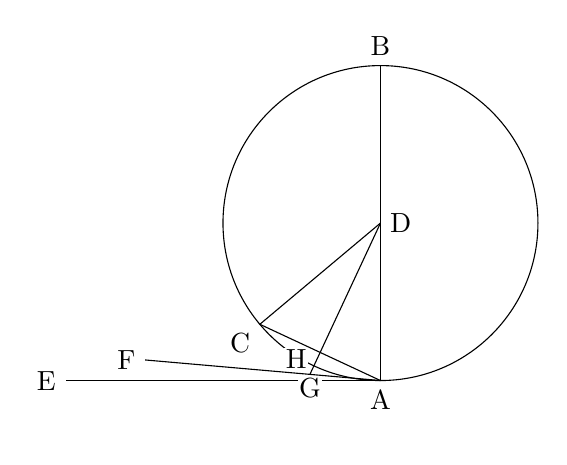
\begin{tikzpicture}
	\coordinate [label=above:B] (B) at (0, 2);
	\coordinate [label=below:A] (A) at (0, -2);
	\coordinate [label=right:D] (D) at (0, 0);
	\coordinate [label=below left:C] (C) at (220:2);
	\coordinate [label=left:E] (E) at (-4, -2);
	\path (0, -2) +(175:3) coordinate [label=left:F] (F);
	\draw (0, 0) circle [radius=2];
	\draw (B) -- (A) -- (E);
	\draw (D) -- (C) -- (A);
	\draw [name path=af] (A) -- (F);
	\path [name path=dh] (D) -- (245:3);
	\draw [name intersections={of=af and dh}] (D) -- (intersection-1) coordinate [label={[label distance=1pt,fill=white,inner sep=0.5pt]below:G}] (G);
	\coordinate [label={[label distance=2pt,fill=white,inner sep=0.5pt,anchor=335]165:H}] (H) at (245:2);
\end{tikzpicture}
}
\end{makeimage}
\end{figure}
\end{center}
\begin{quote}
I say further that the angle of the semicircle contained by the straight line \textit{BA} and the circumference \textit{CHA} is greater than any acute rectilineal angle, and the remaining angle contained by the circumference \textit{CHA} and the straight line \textit{AE} is less than any acute rectilineal angle.
\end{quote}

Not sure what Euclid meant by "the angle contained by\ldots the circumference \textit{CHA}", I tried imagining the segment \textit{CHA} and thus the angle contained by the line \textit{CA} and \textit{BA} or \textit{AE}, but that didn't make any sense.  After thinking on the text a bit longer I gave up and decided to search for the proposition and landed at \htmladdnormallink{this page}{https://mathcs.clarku.edu/~djoyce/java/elements/bookIII/propIII16.html} (whose site I'd come across earlier) which explained that what Euclid was referring to was called a "Horn angle"; that is, Euclid was describing the angle made between a \emph{line} and a \emph{curve}.  Nothing that I'd learned in geometry had prepared me for this; I'd always thought of angles as between straight lines, never between curves, hence I was totally blind-sided by the idea.  The proposition now made sense, though, and I was lucky enough to not have to consider horn angles for the rest of my reading (so far).

\subsection{Epilogue: Generating a Transparent Graph}
The last graph took a surprising amount of effort in order to generate, so I'm going to ramble about it here.  The trick came about in part because of the \textit{G} and \textit{H} labels; unlike the other labels, these needed to mask the lines under them.  The simple solution was to add a \texttt{fill=white} command, but, of course this doesn't quite work on the grayish background of the webpage, but, wait, what's with that background:
\begin{figure}
\includegraphics[scale=0.5]{files/blog/2019_02_21_math_euclid_pt1/2019_02_21_broken.png}
\caption{Figure is produced with a contrasting background.}
\end{figure}
Though I could change the fill to the same color as the webpage background, I didn't know what color that was and worried that future graphs may need more colors that would trigger this issue, so I resolved to find out what was going on and fix it.

I first supplied \texttt{-debug} to the \texttt{latex2html} command-line and learned that the final part of the image processing involves running the \texttt{pnmcrop}, \texttt{ppmquant}, and then \texttt{pnmtopng} commands.  Unfortunately, \LaTeX2html was cleaning the intermediate PNM, PS, and PNG files, but that was remedied by editing the \texttt{latex2html} file's \texttt{cleanup} function to simply return rather than perform clean-up.  Looking at the intermediate files I then noticed that all of the PostScript and PNM files in fact had the same gray background, it was only the PNG images in which the background had (usually) become fully transparent.  For example, here is how the graph relating to Book I, Proposition 47 looks like as a PNM (though it was converted to a PNG for posting's sake):
\begin{figure}
\includegraphics[scale=0.5]{files/blog/2019_02_21_math_euclid_pt1/2019_02_21_workspnm.png}
\caption{PNMs of images that work fine have the same gray background.}
\end{figure}
Looking closer at the commands showed that the \texttt{-trans '#d9d9d9'} option was being passed to \texttt{pnmtopng}, thus it seemed that the gray color was being used as a marker for what would become transparent in the final PNG image, but why wasn't it working for this problem image?  I also took a look at the resulting files with the \texttt{file} command, naming one image "working" and the other "broken" after whether they rendered as per my expectation or not, respectively:
\begin{quote}
\begin{verbatim}
	works.pnm:  Netpbm image data, size = 1032 x 1093, rawbits, pixmap
	broken.pnm: Netpbm image data, size = 643 x 518, rawbits, pixmap
	works.png:  PNG image data, 1032 x 1093, 4-bit colormap, interlaced
	broken.png: PNG image data, 643 x 518, 8-bit grayscale, interlaced
\end{verbatim}
\end{quote}
So the broken image was being converted to a grayscale which had no alpha channel!  I ran the command myself (\texttt{pnmtopng -interlace -trans '#d9d9d9'}) in order to see if I could reproduce the output and, sure enough, ran into the same issue.  I checked the man page for a workaround and noticed that by default the program would use a "nearby" color if the specified transparency color wasn't found, but I could append an \texttt{=} to the color in order to make it match exactly.  When I tried this neither the working image nor the broken image had \emph{any} transparency, and the previously-working image printed the warning \texttt{pnmtopng: specified transparent color not present in palette; ignoring -transparent} as well (the broken image did not print anything); strange that it should only warn for working image, presumably the broken one matched better, but then where was the transparency?!  I figured it must not exist in grayscale images, as they must not have an alpha channel.  At this point I decided to e-mail the soon-to-be-unfortunate program maintainer telling him that I'd run into a bug.  In the meantime I figured out that I could set the fill color with \verb+\definecolor{mycolor}{RGB}{192, 192, 192}+ to make it the same gray as the background and thus cause it to appear transparent as the other, "working", image was, but this workaround was still not satisfying.

The maintainer got back to me and told me that, in fact, the grayscale image does have transparency in it!  Apparently, for images where a single color is designated as transparent, that information is encoded via something called a "\htmladdnormallink{tRNS chunk}{http://www.libpng.org/pub/png/book/chapter08.html#png.ch08.div.5.2}" rather than a separate alpha channel (thus saving space).  He told me that I could check using either \texttt{pngtopam -verbose > /dev/null} or \texttt{pngcheck -v}.  Doing so showed the following:
\begin{quote}
\begin{verbatim}
	File: broken.png (9153 bytes)
	  chunk IHDR at offset 0x0000c, length 13
	    643 x 518 image, 8-bit grayscale, interlaced
	  chunk tRNS at offset 0x00025, length 2
	    gray = 0x00d9
	  chunk IDAT at offset 0x00033, length 8192
	    zlib: deflated, 32K window, default compression
	    rows per pass: 65, 65, 65, 130, 129, 259, 259
	  chunk IDAT at offset 0x0203f, length 878
	  chunk IEND at offset 0x023b9, length 0
	No errors detected in broken.png (5 chunks, 97.3% compression).

	File: works.png (21851 bytes)
	  chunk IHDR at offset 0x0000c, length 13
	    1032 x 1093 image, 4-bit palette, interlaced
	  chunk PLTE at offset 0x00025, length 48: 16 palette entries
	  chunk IDAT at offset 0x00061, length 8192
	    zlib: deflated, 32K window, default compression
	    rows per pass: 137, 137, 137, 274, 273, 547, 546
	  chunk IDAT at offset 0x0206d, length 8192
	  chunk IDAT at offset 0x04079, length 5326
	  chunk IEND at offset 0x05553, length 0
	No errors detected in works.png (6 chunks, 96.1% compression).
\end{verbatim}
\end{quote}
So the broken image did indeed have a transparency value encoded as a tRNS chunk while the working image had a palette entry to designate transparency, but why wasn't it showing as transparent on the broken image?  Were all the image viewers that I tried just buggy?

Then it occurred to me: does \texttt{#d9d9d9} actually map onto an 8-bit grayscale?  I opened the PNG image and noticed that the gray was actually \texttt{#c0c0c0}!  So it had been downscaled, but, wait, it turned out to be the same value in the PNM image... and the PostScript image!  Well, what created the PostScript image?  That turned out to be a DVI file which contained \emph{all} of the images, so it was a bit tricker to analyze.  After digging in \LaTeX2html's source code though I eventually found that the background color was set via the variable \texttt{\$LATEX_COLOR} which was by default \verb+\pagecolor[gray]{.7}+.  By setting this value myself in \texttt{.latex2html-init} to the expected transparency value with \verb+\pagecolor[RGB]{217, 217, 217}+ (the decimal equivalent of the hexadecimal value) and adjusting my workaround to also use said value (never mind that I didn't previously comprehend that I was using \texttt{#c0c0c0} rather than \texttt{#d9d9d9} when I first implemented the workaround) I could then generate a correct image!  In addition, the warning that came from generating a PNG from the PNM file when using the exact transparency specification went away.  Turns out the other images \emph{happened} to work because \texttt{pnmtopng} was selecting the nearby color \texttt{#c0c0c0} when it couldn't find \texttt{#d9d9d9}, but this nearness selection didn't happen when generating a grayscale image, thus causing my problem!

The problem root caused and solution found, I decided to check if there was anywhere I could submit a patch against \LaTeX2html.  Checking my distribution's upstream it appeared that someone had actually taken on maintaining the \htmladdnormallink{program}{https://github.com/latex2html/latex2html/} to some extent, as the original author, Nikos Drakos, was no longer maintaining it.  Before submitting a patch I took a look at the newest version and noticed that a number of significant changes had been made, such as using \texttt{pdflatex} in order to generate images by default.  Slightly daunted, I tried it out, but the results that I got had a black background for all images and made some other changes to the layout of the webpage that I was not particularly keen on.  I tried tweaking the options based on a few of the commits but quickly ran out of patience; I was not trying to port my website to a new version of the tool with breaking changes \emph{and} fix a bug, especially as I'd already dumped so much time into it already.  Before quitting, though, I did notice a \htmladdnormallink{patch}{https://github.com/latex2html/latex2html/commit/02aca89d8c282a8c65d60fcbdd3c6ccf30f4bea8} which appeared to address a similar issue.  Fair enough then, it seemed the problem was already noticed and had a solution; too bad I didn't see it sooner!

Thus the great image conversion transparency saga of early 2019 came to an end.  Hopefully my next blog attempt will run into fewer issues, sheesh!

My thanks to the Netpbm (\texttt{pnmtopng}) maintainer Bryan Henderson for his assistance.


% Pillars of Eternity: Path of the Damned, Act II
\section{2018-11-25 Pillars of Eternity: Path of the Damned, Act II}
At last, part II is done!  The sequel continues to tempt me, but I remain committed to mastering the first game before moving onto the second.

Act II is probably the lengthiest act in the game, consisting of the entire city of Defiance Bay, a journey through the wilderness, Dyrford Village, Engwithian Ruins, and, optionally, most of the Endless Paths; hence in part why it took so long to complete.  That, and work, as I am, alas, not yet retired.

\subsection{Defiance Bay Sidequests}
The first time I entered Defiance Bay the city was rather overwhelming for my completionist nature; how was I to explore every nook and cranny and complete all of the quests?  Talking to a quest-giver often gave quests that lead me to another district, which would quickly tangle me up in a web of half-explored and half-completed areas.  Instead I came up with the following algorithm: explore an entire district, completing all quests that stay within it and other previously-explored areas, then enter a new district and repeat the previous step.  Before completing any quests, however, the first order of business was to grab the awesome summoning trinkets.  The first, "Oaken Scarab Figurine", which summons 3 Wood Beetles, was in a hidden stash near the amphitheatre.  Next, I stole the "Obsidian Lamp Figurine", which summons 3 Shades, from the Vailian Embassy (I would have bought it but they don't offer that option!).  The "Ashwood Cameo Figurine" was being sold by the merchant Lora in the Copperlane merchant district for 15,000 copper; I didn't have the cash to buy it right away, so it had to wait until later.

Figurines in hand, it was time to begin questing.  I went through Copperlane, First Fires, Brackenbury, Ondra's Gift, then finally Heritage Hill.  Since I had gone so deep into the Endless Paths and gained powerful loot and experience, I began to move ahead of the level difficulty, making the journey much easier.  More loot was to come, though; upon completing the first quest for the Crucible Knights (the one that doesn't exclude you from the other factions), I noticed that the smith, Dunstan, sold a pair of boots called "Shod-in-Faith" that would proc "Consecrated Ground" when the wearer was hit by a critical hit.  Since my Monk was having difficulties staying alive, I placed these on my Monk and, when combined with "Fulvano's Amulet", which increases healing received by 25\%, they are insanely powerful, allowing my Monk to profit from damage while not getting beaten down by it.  Further questing in Heritage Hill also gave me the "Iridescent Scarab Figurine", which summons an Adra Beetle, from the family tomb where Saeda was hiding.  The biggest challenge was the lighthouse in Ondra's Gift, but it was nothing an army of figurines couldn't handle:

\begin{figure}
\includegraphics[scale=0.33]{files/blog/2018_11_25_pillars_of_eternity_path_of_the_damned_act_ii/2018_11_25_lighthouse.jpg}
\end{figure}

Amusingly enough, accidentally killing my summoned animat with the adra beetle's "Shocking Blast" gave a little bit of experience.  Having cleared out most of Defiance Bay it was time to progress the main questline a little.

\subsection{Defiance Bay Catacombs}
The catacombs were easy-going as well; I cleared them out without a problem.

\begin{figure}
\includegraphics[scale=0.33]{files/blog/2018_11_25_pillars_of_eternity_path_of_the_damned_act_ii/2018_11_25_catacombs.jpg}
\end{figure}

Having cleared most of Defiance Bay and gained a few levels I next went to dispatch a few ruffians on the road.

\subsection{Bounties}
I find the bounties quite enjoyable.  They are fights where one can go all-out without feeling like they are cheesing it, and, if there's one thing that Pillars is all about, it's epic battles.  First up, the Dweller:

\begin{figure}
\includegraphics[scale=0.33]{files/blog/2018_11_25_pillars_of_eternity_path_of_the_damned_act_ii/2018_11_25_dweller_begin.jpg}
\end{figure}

I began playing around with Aloth's "Minor Grimoire Imprint", but have generally found it too buggy in that it often doesn't actually steal spells when it should.  Regardless, the Dweller went down without much hassle:

\begin{figure}
\includegraphics[scale=0.33]{files/blog/2018_11_25_pillars_of_eternity_path_of_the_damned_act_ii/2018_11_25_dweller_end.jpg}
\end{figure}

Next up was Sly Cidrel.  The battle started out easy enough.

\begin{figure}
\includegraphics[scale=0.33]{files/blog/2018_11_25_pillars_of_eternity_path_of_the_damned_act_ii/2018_11_25_slycidrel_begin.jpg}
\end{figure}

\ldots but it almost became a disaster when my backline was struct by mass confusion.

\begin{figure}
\includegraphics[scale=0.33]{files/blog/2018_11_25_pillars_of_eternity_path_of_the_damned_act_ii/2018_11_25_slycidrel_mid.jpg}
\end{figure}

Flee, Aloth, flee!  "Deleterious Alacrity of Motion" turns out to be useful not just for casting spells but for getting out of harm's way.  A bit of kiting later the confusion wore off and I made short work of the bandits.

\begin{figure}
\includegraphics[scale=0.33]{files/blog/2018_11_25_pillars_of_eternity_path_of_the_damned_act_ii/2018_11_25_slycidrel_end.jpg}
\end{figure}

A bit further north, next to the bear cave from the beginning of the game, was Warchief Iklak and his drakes.

\begin{figure}
\includegraphics[scale=0.33]{files/blog/2018_11_25_pillars_of_eternity_path_of_the_damned_act_ii/2018_11_25_warchiefiklak_begin.jpg}
\end{figure}

I'd begun using Kana's "One Dozen Stood Against the Power of the Saint" chant to help negate the drakes' fear auras; it turns out to be quite powerful.

\begin{figure}
\includegraphics[scale=0.33]{files/blog/2018_11_25_pillars_of_eternity_path_of_the_damned_act_ii/2018_11_25_warchiefiklak_end.jpg}
\end{figure}

Alas, the final bounty was out of reach until Act III, so I decided to continue cleaning my keep's basement instead.

\subsection{The Endless Paths}
It was time once again to take on the adragans.

\begin{figure}
\includegraphics[scale=0.33]{files/blog/2018_11_25_pillars_of_eternity_path_of_the_damned_act_ii/2018_11_25_adragan1.jpg}
\end{figure}

I go for the adragans before the shades and animats due to their blight summons and dominating abilities.

\begin{figure}
\includegraphics[scale=0.33]{files/blog/2018_11_25_pillars_of_eternity_path_of_the_damned_act_ii/2018_11_25_adragan2.jpg}
\end{figure}

Alas, I was not fast enough taking out the adragans and lost Durance along the way.

\begin{figure}
\includegraphics[scale=0.33]{files/blog/2018_11_25_pillars_of_eternity_path_of_the_damned_act_ii/2018_11_25_adragan3.jpg}
\end{figure}

The result was a wipe.  Undeterred, I tried once again.

\begin{figure}
\includegraphics[scale=0.33]{files/blog/2018_11_25_pillars_of_eternity_path_of_the_damned_act_ii/2018_11_25_adragan4.jpg}
\end{figure}

\ldots and managed to succeed!  Alas I forgot to take a screenshot.  Below the blights room is the fampyr room, with the semi-optional boss.  The boss is semi-optional because he's mandatory unless you've learned to speak Engwithian, otherwise you can kill the other fampyrs and skip him; the thing is, though, he wears a plate mail enchanted with "Second Chance", which is quite useful on a tank and is also one of the few enchanted plate mails available in the base game.  Definitely worth killing, but a very tough fight.  I postponed the questline which grants me knowledge of Engwithian specifically so I had good reason to kill him.

\begin{figure}
\includegraphics[scale=0.33]{files/blog/2018_11_25_pillars_of_eternity_path_of_the_damned_act_ii/2018_11_25_fampyr01.jpg}
\end{figure}

Note that I gave my whole party snowcap mushrooms for the extra resistance against the charm and dominated afflictions, as Durance had not yet learned "Prayer Against Treachery".  Also note the two death guards preparing to cast fireball, nevermind the small army of darguls.

\begin{figure}
\includegraphics[scale=0.33]{files/blog/2018_11_25_pillars_of_eternity_path_of_the_damned_act_ii/2018_11_25_fampyr02.jpg}
\end{figure}

The fireballs hurt.  Lots.  They killed most of summons and left my party in rough shape.

\begin{figure}
\includegraphics[scale=0.33]{files/blog/2018_11_25_pillars_of_eternity_path_of_the_damned_act_ii/2018_11_25_fampyr03.jpg}
\end{figure}

The enemies also kept going after Hiravas, making it impossible for him to cast the awesome "Relentless Storm" spell; I kept having to cast "Beetle Shell" in order to prevent a knockout.

\begin{figure}
\includegraphics[scale=0.33]{files/blog/2018_11_25_pillars_of_eternity_path_of_the_damned_act_ii/2018_11_25_fampyr04.jpg}
\end{figure}

At this point my summons were all gone and I was left with quite a few enemies, but that's no reason to give up!

\begin{figure}
\includegraphics[scale=0.33]{files/blog/2018_11_25_pillars_of_eternity_path_of_the_damned_act_ii/2018_11_25_fampyr05.jpg}
\end{figure}

Unfortunately Durance got charmed while Hiravas continued to get pummeled, making healing the latter impossible.

\begin{figure}
\includegraphics[scale=0.33]{files/blog/2018_11_25_pillars_of_eternity_path_of_the_damned_act_ii/2018_11_25_fampyr06.jpg}
\end{figure}

Then the boss got a few quick crits on my Monk, taking him down.

\begin{figure}
\includegraphics[scale=0.33]{files/blog/2018_11_25_pillars_of_eternity_path_of_the_damned_act_ii/2018_11_25_fampyr07.jpg}
\end{figure}

I managed to revive the Monk, but lost Durance in the process.  I also learned to use Aloth's "Ninagauth's Bitter Mooring" to (sort of) control the death guards by inflicting them with a stuck affliction.

\begin{figure}
\includegraphics[scale=0.33]{files/blog/2018_11_25_pillars_of_eternity_path_of_the_damned_act_ii/2018_11_25_fampyr08.jpg}
\end{figure}

Their Fireballs still hurt, though, and I lost the Monk for a final time to one.

\begin{figure}
\includegraphics[scale=0.33]{files/blog/2018_11_25_pillars_of_eternity_path_of_the_damned_act_ii/2018_11_25_fampyr09.jpg}
\end{figure}

My main healers and Monk down, and Aloth nearly out of spells, it wasn't long until the subsequent wipe.  Ouch.  Even some of the party's \emph{health} is in red.  I considered re-working my strategy a little.  Since the Fireballs did tons of damage, I decided to craft a "Potion of Bulwark Against The Elements" potion for each character; this potion couldn't be taken before the battle, so I decided to take it as soon as the battle started.  I also had the figurines summon as close to the enemies as possible (hopefully out of fireball range).

\begin{figure}
\includegraphics[scale=0.33]{files/blog/2018_11_25_pillars_of_eternity_path_of_the_damned_act_ii/2018_11_25_fampyr10.jpg}
\end{figure}

To my great consternation my team was not able to chug the potions before getting blasted by fireballs, the blast interrupted their chugging, and they knocked out Hiravas!  I almost rage-restarted the battle at this point, but instead decided to re-try taking the potions and revive Hiravas.

\begin{figure}
\includegraphics[scale=0.33]{files/blog/2018_11_25_pillars_of_eternity_path_of_the_damned_act_ii/2018_11_25_fampyr11.jpg}
\end{figure}

Finally, I managed to get Relentless Storm cast, then managed to anchor a death guard with Ninagauth's Bitter Mooring.

\begin{figure}
\includegraphics[scale=0.33]{files/blog/2018_11_25_pillars_of_eternity_path_of_the_damned_act_ii/2018_11_25_fampyr12.jpg}
\end{figure}

Despite the brutal start, the stuns from Hiravas made a huge difference and I managed to secure a victory over the boss, netting his sweet plate mail in the process.

Though the following floors would not be easy, my past experience was that no fight ahead would be as tough as the last one.  Since that would lead to a sad dearth of screenshots, I decided to take one for the most intense fight that the floor offered.

Level 9 is probably best described as the torture floor given its medieval-style torture implements and spiked floor.

\begin{figure}
\includegraphics[scale=0.33]{files/blog/2018_11_25_pillars_of_eternity_path_of_the_damned_act_ii/2018_11_25_paths_l09.jpg}
\end{figure}

Crystal eaters are squishy but deadly with their petrify affliction and ability to cast "Ninagauth's Freezing Pillar", but nothing I couldn't handle.

\begin{figure}
\includegraphics[scale=0.33]{files/blog/2018_11_25_pillars_of_eternity_path_of_the_damned_act_ii/2018_11_25_paths_l10.jpg}
\end{figure}

Level 10 is rather short and indescript.  Durance's "Prayer Against Imprisonment" (sp?) was extremely handy against Cean Gwlas, as it prevented my party from being paralyzed and beaten.

\begin{figure}
\includegraphics[scale=0.33]{files/blog/2018_11_25_pillars_of_eternity_path_of_the_damned_act_ii/2018_11_25_paths_l11_1.jpg}
\end{figure}

Level 11 is the dank cave level with the aggravating spores that like to control half of the party (literally).

\begin{figure}
\includegraphics[scale=0.33]{files/blog/2018_11_25_pillars_of_eternity_path_of_the_damned_act_ii/2018_11_25_paths_l11_2.jpg}
\end{figure}

The solution, of course, is to just summon more minions, as the bastards can't control them all!

\begin{figure}
\includegraphics[scale=0.33]{files/blog/2018_11_25_pillars_of_eternity_path_of_the_damned_act_ii/2018_11_25_paths_l12.jpg}
\end{figure}

The strange greenish cave on level 12 (with the neutral vithrack) presented me with a problem when I didn't position my party properly and almost got killed by the frost and petrification.  Thankfully I paused to study Aloth's grimoire and then tried out "Call to Slumber" to great success; it is a save versus will, which is often weak, and afflicts the enemy with unconsciousness, giving -40 deflection, which is incredibly powerful, allowing my monk to tear through enemies afflicted by it.

\begin{figure}
\includegraphics[scale=0.33]{files/blog/2018_11_25_pillars_of_eternity_path_of_the_damned_act_ii/2018_11_25_paths_l13.jpg}
\end{figure}

The final level one can get to without learning Engwithian, level 13, is mostly straightforward.  The adra animats aren't that tough, but the fight against \emph{five} Cean Gwla proved difficult, even with "Prayer Against Imprisonment", as the damage from their wail and regular attacks is quite powerful.  Nonetheless I managed to take them out before finally being blocked from going deeper.  It was time to go back and finish the main quests in Defiance Bay.

\subsection{The Sanitarium and Teir Nowneth}
At this point the extra levels and gear had practically allowed me to undergo apotheosis.

\begin{figure}
\includegraphics[scale=0.33]{files/blog/2018_11_25_pillars_of_eternity_path_of_the_damned_act_ii/2018_11_25_sanitarium.jpg}
\end{figure}

I cleared the sanitarium without a problem.

\begin{figure}
\includegraphics[scale=0.33]{files/blog/2018_11_25_pillars_of_eternity_path_of_the_damned_act_ii/2018_11_25_teirnowneth.jpg}
\end{figure}

Same with the tower in Heritage Hill, and the unnerving conversation with Icantha, which meant I could push a little deeper into the Endless Paths!  Actually, I forgot to take a screenshot of these so I did it after the fact using an old save.  Don't tell!

\subsection{The Throne Room and Od Nua}
Past the sealed door in the Endless Paths is the throne room of Od Nua, though not Od Nua himself.

\begin{figure}
\includegraphics[scale=0.33]{files/blog/2018_11_25_pillars_of_eternity_path_of_the_damned_act_ii/2018_11_25_paths_l13_2.jpg}
\end{figure}

The battle is pretty intense, but nothing particularly challenging awaits in this room.

\begin{figure}
\includegraphics[scale=0.33]{files/blog/2018_11_25_pillars_of_eternity_path_of_the_damned_act_ii/2018_11_25_paths_l14.jpg}
\end{figure}

Finally comes the encounter with Od Nua himself on level 14, leaving one final level.  I cleared the trash on level 15, but dared not even try to fight the Master Below until max level.  No, instead I would save him for last, as he's possibly more difficult than the proper final boss.  So, back onto the main questline it was.

\subsection{Through Death's Gate}
Before heading straight to Dyrford Village I like to detour south of Defiance Bay and clear the relevant areas.

\begin{figure}
\includegraphics[scale=0.33]{files/blog/2018_11_25_pillars_of_eternity_path_of_the_damned_act_ii/2018_11_25_searingfalls.jpg}
\end{figure}

Searing Falls with its drakes (and distinct lack of anything I'd consider a "fall") is the first destination.

\begin{figure}
\includegraphics[scale=0.33]{files/blog/2018_11_25_pillars_of_eternity_path_of_the_damned_act_ii/2018_11_25_cailthesilent.jpg}
\end{figure}

Then comes the lava cave with Cail the Silent, a drake of moderate strength, easily crushed by my superior levels.

\begin{figure}
\includegraphics[scale=0.33]{files/blog/2018_11_25_pillars_of_eternity_path_of_the_damned_act_ii/2018_11_25_pearlwoodbluff.jpg}
\end{figure}

After that is the cliff of Pearlwood Bluff with a few drakes, menpwgra, and a hidden cave.  Around this time I realized the glory of "Vulnerable Attack" on my Monk, which slows attacks down by 20\% but gives 5 Damage Reduction (DR), extremely useful for heavily-armored foes.

\begin{figure}
\includegraphics[scale=0.33]{files/blog/2018_11_25_pillars_of_eternity_path_of_the_damned_act_ii/2018_11_25_dyrfordvillage.jpg}
\end{figure}

Detour complete, it was on to Dyrford Village via Stormwall George (the latter of which I forgot to screenshot).

\begin{figure}
\includegraphics[scale=0.33]{files/blog/2018_11_25_pillars_of_eternity_path_of_the_damned_act_ii/2018_11_25_dyrfordcrossing.jpg}
\end{figure}

Quests in hand I proceeded to clear out Dyrford Crossing and its cave, taking Korgrak as a hireling to defend my keep.

\begin{figure}
\includegraphics[scale=0.33]{files/blog/2018_11_25_pillars_of_eternity_path_of_the_damned_act_ii/2018_11_25_dyrfordruins.jpg}
\end{figure}

The Dryford Ruins which had been made into a Skaenenite temple were long, but I managed to clear that rat's nest in a single rest.

\begin{figure}
\includegraphics[scale=0.33]{files/blog/2018_11_25_pillars_of_eternity_path_of_the_damned_act_ii/2018_11_25_cliabanrilag1.jpg}
\end{figure}

With the cruel cultists dead it was time trespass on the Engwithian ruins of Cliaban Rilag for the Greater Good.

\begin{figure}
\includegraphics[scale=0.33]{files/blog/2018_11_25_pillars_of_eternity_path_of_the_damned_act_ii/2018_11_25_cliabanrilag2.jpg}
\end{figure}

The fights were not difficult, but the scenery was gorgeous.

\begin{figure}
\includegraphics[scale=0.33]{files/blog/2018_11_25_pillars_of_eternity_path_of_the_damned_act_ii/2018_11_25_cliabanrilag3.jpg}
\end{figure}

\ldots and the destination was reached without much problem, though I did almost require a rest.

\subsection{The Hearing}
Information being gathered from the main quests it was time to intrude on the animancy hearings.  I went with the Crucible Knights as The Dozens are a bit overzealous and The Doemenel are straight dicks.

\begin{figure}
\includegraphics[scale=0.33]{files/blog/2018_11_25_pillars_of_eternity_path_of_the_damned_act_ii/2018_11_25_hearing.jpg}
\end{figure}

From there it was straightforward to the end of Act II!

\subsection{Brief Analysis}
Much of the challenge in this act was diminished by out-leveling many of the areas, though the bosses in the Endless Paths were extra difficult at a lower level in order to compensate.  With regards to the party composition and roles, Kana grew quite nicely into his role of off-tank, while Eder became a walking brick.  Hiravas turned into a Crowd Control (CC) master with "Relentless Storm", as did Aloth with "Call to Slumber".  My Monk became a self-perpetuating death machine with his healing boots, and Durance, well, he didn't gain any particularly new or unexpected powers, but he was already a bad-ass healer and entertaining cynic.  Everything came together quite nicely, and it looks like this team will make it through to the end.


% 4.14-4.18 Linux Kernel Upgrade Networking Woes
\section{2018-11-11 4.14-4.18 Linux Kernel Upgrade Networking Woes}
I seem to be having bad luck with kernel upgrades.  Traditionally, upgrades have worked out smoothly\ldots until, of course, I started this blog, at which point they started providing me with blog material.  Normally there wouldn't be anything of particular interest in this blog besides giving an example of thought process for those unfamiliar with it, but necessity caused me to come up with a novel, at least in my experience, hack for manual testing.  The rest was legwork.

\subsection{The Saga Begins}
I chose to use the latest stable release rather than a newer Long Term Support (LTS) version of my current kernel.  Everything began normally: downloading source, verifying the signature, updating the config with \texttt{make oldconfig}, compiling, installing, and even booting the kernel, except, after booting the kernel I didn't get an IP address.  Re-running the service gave me an IP address, but then running \texttt{ssh} would just hang indefinitely.  I booted into the old kernel (always keep backups) and networking started working again.  Something was broken (\htmladdnormallink{use the latest stable release, he said}{http://kroah.com/log/blog/2018/08/24/what-stable-kernel-should-i-use/})!

The first step was to contact the appropriate people with a bug report.  The kernel source code contained a nice how-to at \texttt{Documentation/admin-guide/reporting-bugs.rst}; this included a format for the bug report as well as a pointer to a script, \texttt{scripts/get_maintainer.pl}, which gave me names and e-mail addresses to submit the bug report to.  So I gathered the data, placed it into the bug report format, and fired off an e-mail.

Not content to simply wait for the maintainers to look at my report, I decided to do a little digging to see if I could find which commit broke networking.  Since I had moved from \texttt{4.14.12} to \texttt{4.18.5} and the latest upstream at the time was \texttt{4.19-rc3} it seemed prudent to try the latest \texttt{-rc} kernel to see if the bug had been fixed.  To my surprise, it worked!  In order to compare apples to apples I then tried the \texttt{4.18} version, which failed.  It seemed that the \texttt{4.18} stable kernel series was missing a patch from the \texttt{4.19} series.

My first approach was to simply \texttt{git log | grep} for my driver, \texttt{r8169}, and look for relevant fixes.  After I had counted 9 relevant commits with many more to go, and realized that each commit would require 2 compilations (one to test if networking is fixed on the commit, another to test that it is broken before the commit), decided that a better method would be to run a \texttt{git bisect} on the source in order to find the fix.

Now, somehow, presumably post-workday delirium, I got it into my head that, when bisecting, using \texttt{good} and \texttt{bad} for descriptive attributes wasn't good enough; thankfully \texttt{git} entertained my delirium and allowed me to rename \texttt{good} to \texttt{fixed} and \texttt{bad} to \texttt{broken} by using \texttt{git bisect start \verb$-$-term-good=fixed \verb$-$-term-bad=broken}, then marking them with \texttt{git bisect fixed} or \texttt{git bisect broken} as needed.

The problem with trying to do this, though, is that each kernel compilation took about half an hour and a manual reboot of my system in order to run the test.  Since I was doing this in my free time after work and in-between getting ready for the next day this meant firing off a single compilation when I got home and testing it right before bed.  This dragged out the process over many days, and, as I honed in on the final commit it seemed to be in the wrong location (the nearby fixes were for an unrelated driver), and, upon testing it, found that the commit I'd honed in on was indeed incorrect (networking was still broken, though I'd run into two fixed commits earlier).  One thing had become clear: I had fucked up.

Thankfully I had been smart enough to take notes and save all of my kernels and their configurations in case this had happened.  Since I wasn't sure what to do at this point I began to peruse the \texttt{git-bisect} man page and found the useful \texttt{git bisect log} to show me what I had marked, and, indeed, I had missed a commit in my logs (though I had thankfully saved the kernel).  Alas, testing the commit showed that my bisect choices were correct; my notes had missed a single entry but were otherwise accurate.  Thus I was left with the annoying task of running through each kernel and checking them for the bug based on my list:
\begin{quote}
\begin{verbatim}
	54dbe75bbf1e - broken
	307797159ac2 - broken
	ee090756962c - broken
	d972604f6f87 - broken
	c81c7012e0c7 - fixed
	2a8a2b7c49d6 - broken
	aba16dc5cf93 - broken
	cf1acec008f8 - fixed
	ac4a5b52f597 - broken
	1eb43fc75448 - broken
	785e76d7a205 - broken
	43f8b22450f0 - broken
	c08eebad4ac5 - broken
	a9910c088647 - broken
\end{verbatim}
\end{quote}
Before doing this, however, I decided to get smart: it had become apparent after much testing that judging whether or not networking was working from whether or not I received a DHCP lease during system initialization was only accurate about 90\% of the time for whatever reason, so I wrote a quick test that would work all of the time using \texttt{ping -c 3}.  Test in hand, running through the pre-compiled kernels was quite fast and I quickly learned that commit \texttt{cf1acec008f8} was actually \texttt{broken}, not \texttt{fixed}.

Fantastic as it was to find the broken commit, I was still left with a big problem: this process was taking forever (and I'd had a week vacation to slow it all down on top of that) and compiling another 6 kernels, since the ones past \texttt{cf1acec008f8} were now irrelevant) would take another week at least.  From perusing the logs I'd learned earlier about the \texttt{git bisect run} command which could automate testing when provided with the appropriate script, but there were multiple problems with that: first, I had to boot the machine into the kernel under test, which would kill the automated bisection; second, even if I could automatically reboot, the test would hang when trying to decrypt my hard-drive; third, I selected a few non-default options during kernel configuration and it wasn't clear how to programmatically select them.  The third problem was feasibly solvable, the first one might be solvable but would require a non-trivial amount of work, and the second one seemed impossible to solve without an unacceptable security compromise.  Automation was out of the question.

\subsection{Forward Compilation}
"Necessity is the mother of all invention" as the old saying goes.  The (only) useful thing about refusing to give up using my Pentium 4 is that it necessitates finding clever solutions for problems rather than \htmladdnormallink{throwing more compute power at terrible code}{https://pxlnv.com/blog/bullshit-web/}.

In this case my problem was that kernel compilation took half an hour and testing couldn't be automated, thus it took many hours to compile and run tests.  Yet I was absent sleeping or working most of the day while my machine idled, but how was I to put that time to good use?  I couldn't \emph{know} which kernel to compile next\ldots if only I could \emph{speculate} which kernel to compile I could \emph{pre-compile} it while I was at work then knock out two tests in short order.  Alas, I had no means of speculation as both possibilities were equally likely!  Then it struck me: why speculate?  I could instead compile \emph{both} kernels if they were equally likely and then \emph{discard} the unneeded one, thus I'd be enabled to perform two tests at once without the need to speculate.  Indeed, this logic could be extended to 3, 4, or even more tests!  Eureka!

As a visualization, consider bisecting the following theoretical series of commits named "1" to "64" after their chronological order; this would take 6 steps and can be represented as a binary tree:
\begin{center}
\begin{makeimage}
\reflectbox{\reflectbox{% _THIS_ exists because otherwise LaTeX2HTML can't figure out where and how to crop the damn image.
\begin{forest}
[32
	[16,edge={green!60!black}
		[8,edge={green!60!black}
			[4,edge={green!60!black}
				[2,edge={green!60!black}
					[1,edge={green!60!black}] {\node [rectangle,draw=orange,fit=()] {};}
					[3,edge={red!80!black}] {\node [rectangle,draw=orange,fit=()] {};}
				] {\node [rectangle,draw=orange,fit=()] {};}
				[6,edge={red!80!black}
					[5,edge={green!60!black}] {\node [rectangle,draw=orange,fit=()] {};}
					[7,edge={red!80!black}] {\node [rectangle,draw=orange,fit=()] {};}
				] {\node [rectangle,draw=orange,fit=()] {};}
			] {\node [rectangle,draw=orange,fit=()] {};}
			[12,edge={red!80!black}
				[10,edge={green!60!black}
					[9,edge={green!60!black}] {\node [rectangle,draw=orange,fit=()] {};}
					[11,edge={red!80!black}] {\node [rectangle,draw=orange,fit=()] {};}
				] {\node [rectangle,draw=orange,fit=()] {};}
				[14,edge={red!80!black}
					[13,edge={green!60!black}] {\node [rectangle,draw=orange,fit=()] {};}
					[15,edge={red!80!black}] {\node [rectangle,draw=orange,fit=()] {};}
				] {\node [rectangle,draw=orange,fit=()] {};}
			] {\node [rectangle,draw=orange,fit=()] {};}
		] {\node [rectangle,draw=orange,fit=()] {};}
		[24,edge={red!80!black}
			[20,edge={green!60!black}
				[18,edge={green!60!black}
					[17,edge={green!60!black}] {\node [rectangle,draw=orange,fit=()] {};}
					[19,edge={red!80!black}] {\node [rectangle,draw=orange,fit=()] {};}
				] {\node [rectangle,draw=orange,fit=()] {};}
				[22,edge={red!80!black}
					[21,edge={green!60!black}] {\node [rectangle,draw=orange,fit=()] {};}
					[23,edge={red!80!black}] {\node [rectangle,draw=orange,fit=()] {};}
				] {\node [rectangle,draw=orange,fit=()] {};}
			] {\node [rectangle,draw=orange,fit=()] {};}
			[28,edge={red!80!black}
				[26,edge={green!60!black}
					[25,edge={green!60!black}] {\node [rectangle,draw=orange,fit=()] {};}
					[27,edge={red!80!black}] {\node [rectangle,draw=orange,fit=()] {};}
				] {\node [rectangle,draw=orange,fit=()] {};}
				[30,edge={red!80!black}
					[29,edge={green!60!black}] {\node [rectangle,draw=orange,fit=()] {};}
					[31,edge={red!80!black}] {\node [rectangle,draw=orange,fit=()] {};}
				] {\node [rectangle,draw=orange,fit=()] {};}
			] {\node [rectangle,draw=orange,fit=()] {};}
		] {\node [rectangle,draw=orange,fit=()] {};}
	] {\node [rectangle,draw=orange,fit=()] {};}
	[48,edge={red!80!black}
		[40,edge={green!60!black}
			[36,edge={green!60!black}
				[34,edge={green!60!black}
					[33,edge={green!60!black}] {\node [rectangle,draw=orange,fit=()] {};}
					[35,edge={red!80!black}] {\node [rectangle,draw=orange,fit=()] {};}
				] {\node [rectangle,draw=orange,fit=()] {};}
				[38,edge={red!80!black}
					[37,edge={green!60!black}] {\node [rectangle,draw=orange,fit=()] {};}
					[39,edge={red!80!black}] {\node [rectangle,draw=orange,fit=()] {};}
				] {\node [rectangle,draw=orange,fit=()] {};}
			] {\node [rectangle,draw=orange,fit=()] {};}
			[44,edge={red!80!black}
				[42,edge={green!60!black}
					[41,edge={green!60!black}] {\node [rectangle,draw=orange,fit=()] {};}
					[43,edge={red!80!black}] {\node [rectangle,draw=orange,fit=()] {};}
				] {\node [rectangle,draw=orange,fit=()] {};}
				[46,edge={red!80!black}
					[45,edge={green!60!black}] {\node [rectangle,draw=orange,fit=()] {};}
					[47,edge={red!80!black}] {\node [rectangle,draw=orange,fit=()] {};}
				] {\node [rectangle,draw=orange,fit=()] {};}
			] {\node [rectangle,draw=orange,fit=()] {};}
		] {\node [rectangle,draw=orange,fit=()] {};}
		[56,edge={red!80!black}
			[52,edge={green!60!black}
				[50,edge={green!60!black}
					[49,edge={green!60!black}] {\node [rectangle,draw=orange,fit=()] {};}
					[51,edge={red!80!black}] {\node [rectangle,draw=orange,fit=()] {};}
				] {\node [rectangle,draw=orange,fit=()] {};}
				[54,edge={red!80!black}
					[53,edge={green!60!black}] {\node [rectangle,draw=orange,fit=()] {};}
					[55,edge={red!80!black}] {\node [rectangle,draw=orange,fit=()] {};}
				] {\node [rectangle,draw=orange,fit=()] {};}
			] {\node [rectangle,draw=orange,fit=()] {};}
			[60,edge={red!80!black}
				[58,edge={green!60!black}
					[57,edge={green!60!black}] {\node [rectangle,draw=orange,fit=()] {};}
					[59,edge={red!80!black}] {\node [rectangle,draw=orange,fit=()] {};}
				] {\node [rectangle,draw=orange,fit=()] {};}
				[62,edge={red!80!black}
					[61,edge={green!60!black}] {\node [rectangle,draw=orange,fit=()] {};}
					[63,edge={red!80!black}] {\node [rectangle,draw=orange,fit=()] {};}
				] {\node [rectangle,draw=orange,fit=()] {};}
			] {\node [rectangle,draw=orange,fit=()] {};}
		] {\node [rectangle,draw=orange,fit=()] {};}
	] {\node [rectangle,draw=orange,fit=()] {};}
%] {\node [rectangle,draw=orange,fill=green,fill opacity=0.2,draw opacity=0.2,fit=()] {};} % FIXME: Transparency not working.  Works via 'pdflatex', wtf?
% https://tex.stackexchange.com/questions/172764/opacity-and-transparency  % Doesn't actually work, WTF?
% https://tex.stackexchange.com/questions/399767/pstricks-and-opacity-with-gradient-filling?noredirect=1
] {\node [rectangle,draw=orange,fit=()] {};}
% Left side arrow thingy.
\node(leftbox) at ($(current bounding box.west) - (0.75, 0)$){$6$};
\path (current bounding box.north west) -- (current bounding box.north) node(topline){};
\draw[->] (leftbox) -- (leftbox |- topline);
\path (current bounding box.south west) -- (current bounding box.south) node(botline){};
\draw[->] (leftbox) -- (leftbox |- botline);
\end{forest}
}}
\end{makeimage}
\end{center}
A bisection would travel downward along the tree, following the green line on a \texttt{fixed} commit and the red line on a \texttt{broken} commit.  The orange boxes represent the number of commits tested in a single "session"; the default is to test a single commit in a single session, represented by a orange box existing around each individual commit; it would thus take 6 sessions to traverse to the bottom of the tree.  Using forward compilation to compile 3 commits worth of kernels at once then produces the following graph:

\begin{center}
\begin{makeimage}
\reflectbox{\reflectbox{% _THIS_ exists because otherwise LaTeX2HTML can't figure out where and how to crop the damn image.
\begin{forest}
[32
	[16,edge={green!60!black}
		[8,edge={green!60!black}
			[4,edge={green!60!black}
				[2,edge={green!60!black}
					[1,edge={green!60!black}]
					[3,edge={red!80!black}]
				]
				[6,edge={red!80!black}
					[5,edge={green!60!black}]
					[7,edge={red!80!black}]
				]
			] {\node [rectangle,draw=orange,fit=()(!11)(!22)] {};}
			[12,edge={red!80!black}
				[10,edge={green!60!black}
					[9,edge={green!60!black}]
					[11,edge={red!80!black}]
				]
				[14,edge={red!80!black}
					[13,edge={green!60!black}]
					[15,edge={red!80!black}]
				]
			] {\node [rectangle,draw=orange,fit=()(!11)(!22)] {};}
		]
		[24,edge={red!80!black}
			[20,edge={green!60!black}
				[18,edge={green!60!black}
					[17,edge={green!60!black}]
					[19,edge={red!80!black}]
				]
				[22,edge={red!80!black}
					[21,edge={green!60!black}]
					[23,edge={red!80!black}]
				]
			] {\node [rectangle,draw=orange,fit=()(!11)(!22)] {};}
			[28,edge={red!80!black}
				[26,edge={green!60!black}
					[25,edge={green!60!black}]
					[27,edge={red!80!black}]
				]
				[30,edge={red!80!black}
					[29,edge={green!60!black}]
					[31,edge={red!80!black}]
				]
			] {\node [rectangle,draw=orange,fit=()(!11)(!22)] {};}
		]
	]
	[48,edge={red!80!black}
		[40,edge={green!60!black}
			[36,edge={green!60!black}
				[34,edge={green!60!black}
					[33,edge={green!60!black}]
					[35,edge={red!80!black}]
				]
				[38,edge={red!80!black}
					[37,edge={green!60!black}]
					[39,edge={red!80!black}]
				]
			] {\node [rectangle,draw=orange,fit=()(!11)(!22)] {};}
			[44,edge={red!80!black}
				[42,edge={green!60!black}
					[41,edge={green!60!black}]
					[43,edge={red!80!black}]
				]
				[46,edge={red!80!black}
					[45,edge={green!60!black}]
					[47,edge={red!80!black}]
				]
			] {\node [rectangle,draw=orange,fit=()(!11)(!22)] {};}
		]
		[56,edge={red!80!black}
			[52,edge={green!60!black}
				[50,edge={green!60!black}
					[49,edge={green!60!black}]
					[51,edge={red!80!black}]
				]
				[54,edge={red!80!black}
					[53,edge={green!60!black}]
					[55,edge={red!80!black}]
				]
			] {\node [rectangle,draw=orange,fit=()(!11)(!22)] {};}
			[60,edge={red!80!black}
				[58,edge={green!60!black}
					[57,edge={green!60!black}]
					[59,edge={red!80!black}]
				]
				[62,edge={red!80!black}
					[61,edge={green!60!black}]
					[63,edge={red!80!black}]
				]
			] {\node [rectangle,draw=orange,fit=()(!11)(!22)] {};}
		]
	]
] {\node [rectangle,draw=orange,fit=()(!11)(!22)] {};}
% Left side arrow thingy.
\node(leftbox) at ($(current bounding box.west) - (0.75, 0)$){$6$};
\path (current bounding box.north west) -- (current bounding box.north) node(topline){};
\draw[->] (leftbox) -- (leftbox |- topline);
\path (current bounding box.south west) -- (current bounding box.south) node(botline){};
\draw[->] (leftbox) -- (leftbox |- botline);
\end{forest}
}}
\end{makeimage}
\end{center}
In this case it takes a total of 2 sessions rather than 6 to work down the tree.  The downside, of course, is that the number of compilations grows \emph{exponentially} with respect to the number of tests to be run; 7 kernels in order to test 3 commits, and 14 kernels to test the tree.  Trying to jam the entire tree into a single session (an orange box around the entire tree) would require compiling all 64 kernels.

Mathematically, the number of tests \texttt{n} that can be run over a given time period \texttt{t} is given by taking the floor of the base 2 logarithm of \texttt{t} divided by average time of compilation \texttt{c}:
\begin{center}
\begin{makeimage}
	$n = \left \lfloor \log_2(\frac{t}{c}) \right \rfloor$
\end{makeimage}
\end{center}
In my case, 30-minute compilations with a 20-hour compilation period meant 5 tests could be done in a day!  While this is no academic breakthrough due to its usefulness being limited by exponential growth (a 40-hour compilation period would only give 6 tests), the ability to run 5 tests at once is a huge improvement over running tests one at a time.

\subsection{The Final Stretch}
Excited to try my new technique, I was still delayed by the necessity of automating kernel configuration.  Someone suggested that I try using the \texttt{MIN_CONFIG} option of \texttt{tools/testing/ktest/ktest.pl}.  I quickly found the tool to be rather unwieldy for my relatively simple task; this was clearly a tool meant for much more than to apply a simple configuration and build.  I figured out enough of the tool to have it read my configuration file and apply the minimum configuration, but it then tried to configure \emph{again} and erred out claiming that the directory was "not clean".  Impatient, I decided to simply use \texttt{make olddefconfig}; although not entirely accurate it would most likely be enough for my current issue.

Configuration automation in hand I wrote a quick test script and, after a couple of tries, of course, was able to crank out 2 tests worth of kernels, and another 4 tests (the remaining amount) of kernels the next day while I was at work.  Below is a (simplified) version of the script I was able to use:
\begin{quote}
\begin{verbatim}
forward_compile() {
	local commit=$(git log --oneline -n 1 | cut -f 1 -d ' ')
	local log="${LOG}-${commit}"
	# Build kernel.
	# Save results.
	# Compile forward.
	if [ $1 -lt 1 ]; then
		return
	fi
	git bisect log > "${log}"
	git bisect fixed
	forward_compile $(($1 - 1))
	git bisect replay "${log}"
	git bisect broken
	forward_compile $(($1 - 1))
	git bisect replay "${log}"
}
RESULTS="fwdcmpl"
LOG="${RESULTS}/.tmp_bisect_log"
# Parse arguments.
if [ $# -lt 1 ]; then
	echo "USAGE: $0 DEPTH"
	echo "  DEPTH: Tree depth to traverse (2^DEPTH builds will be done)."
	exit 1
fi
# Perform forward compilation.
forward_compile $1
\end{verbatim}
\end{quote}
I was lucky that, during the second run, there were exactly 8 commits left so I did not need to test corner-cases.  Thus I was able to finish testing 6 kernels in two days rather than six, giving me the following list:
\begin{quote}
\begin{verbatim}
	54dbe75bbf1e - broken
	307797159ac2 - broken
	ee090756962c - broken
	d972604f6f87 - broken
	c81c7012e0c7 - fixed
	2a8a2b7c49d6 - broken
	aba16dc5cf93 - broken
	cf1acec008f8 - broken
	15c480efab01 - broken
	6e0bb04d0e4f - fixed
	6a5d39aa9ac2 - broken
	9a07efa9aea2 - broken
	31fabbee8f5c - fixed
	05212ba8132b - fixed
\end{verbatim}
\end{quote}

Alas, it had taken me so long to run all of these tests that the latest stable kernel had moved all the way to \texttt{4.18.14}.  I decided to test this kernel, only to find that networking now worked again!  Someone else must have discovered the bug and backported the patch before I could, the bastard!  My efforts to find the bug fix were thus rendered futile, but at least I learned a useful trick along the way.

I never did hear back from the maintainers, though I did update them letting them know that the bug had been fixed; annoyingly, my message to the mailing list was rejected with the error "\texttt{Your address is not liked source for email}".  Rude!  Things were working again, though, and I wasn't keen on fighting the mailing list at this point, especially when I could be generating visuals for this blog\ldots hopefully I don't need to upgrade my kernels before I finish writing it.


\section{2018-10-07 From Brainpool to Mindmush in OpenSSL}
I\label{2019-10-07-brainpool} have a series of \htmladdnormallink{tests}{https://github.com/clinew/inspircdtests} which attempt to connect to an SSL/TLS-enabled service; the tests use different types of cryptography: RSA, DSA, and EC.  When I began testing with the OpenSSL 1.1.0 series instead of the 1.0.1 series, the test which uses EC started to return an "unknown" result rather than "pass" or "fail".  Looking at the client output showed the following error message: \texttt{140379411924736:error:1409441A:SSL routines:ssl3_read_bytes:tlsv1 alert decode error:ssl/record/rec_layer_s3.c:1399:SSL alert number 50}; the server output wasn't particularly helpful: \texttt{SOCKET: Error on FD 8 - 'Read Error'}.

This looked pretty bad, so I took some time to re-examine the test; it generates an elliptic curve using the \texttt{brainpoolP512t1} curve, which I selected through a rigorous process of running \texttt{openssl ecparam -list_curves} and then just picking one arbitrarily.  The certificate is then signed by the server's trusted root authority and then finally passed to the server by the client, at which point the protocol error occurs.  There didn't seem to be any particular wrongdoing on my end, so I filed a \htmladdnormallink{bug}{https://github.com/inspircd/inspircd/issues/1464} against the service.

The maintainer got back to me pointing to a \htmladdnormallink{bug}{https://github.com/openssl/openssl/issues/6332} filed against OpenSSL in which the project's maintainer responded that it was not possible to use the \texttt{brainpoolP512t1} curve as it had not been assigned a number by the Internet Assigned Numbers Authority (IANA).  But, wait a second, it \emph{had} worked on the older, 1.0.1 series, and upon closer inspection, the filer was \emph{also} using the 1.0.1 series, \emph{and} their error messages were different than mine.  After digging a little deeper I realized that they were using EC for the \emph{server} certificate, while I was using it for the \emph{client}.  From the ticket I was able to reproduce their version of the issue on both the 1.0.1 series and the 1.1.0 series with the following commands:

\begin{quote}
\begin{verbatim}
	openssl ecparam -out eckey.pem -name brainpoolP512t1 -genkey
	openssl req -x509 -new -key eckey.pem -out eccert.pem -subj "/CN=EC-SHA512/"
	openssl s_server -accept 415 -cert eccert.pem -key eckey.pem -4
	openssl s_client -connect 127.0.0.1:415
\end{verbatim}
\end{quote}

This did not, however, explain why I had \emph{ever} been able to connect using EC in the client certificate and my brain was starting to turn to mush trying to figure out what facts might cause such inconsistent behaviour.  Configuring the service was proving to be tricky and I wanted to test against a known-correct implementation, so I decided to see if I could reproduce the client error by the command-line OpenSSL utilities.  I began by generating keys and self-signed certificates:

\begin{quote}
\begin{verbatim}
	openssl ecparam -out eckey.pem -name brainpoolP512t1 -genkey
	openssl req -x509 -new -key eckey.pem -out eccert.pem -subj "/CN=EC-SHA512/"
	openssl genrsa -out rsakey.pem 4096
	openssl req -key rsakey.pem -new -x509 -days 7200 -sha512 -out rsacert.pem -subj '/CN=RSA/'
\end{verbatim}
\end{quote}

\ldots then attempted to connect to the server while using EC in the client certificate:

\begin{quote}
\begin{verbatim}
        openssl s_server -accept 415 -cert rsacert.pem -key rsakey.pem -4
	openssl s_client -cert eccert.pem -key eckey.pem -connect 127.0.0.1:415
\end{verbatim}
\end{quote}

To my great consternation, this worked on \emph{both} OpenSSL series.  After some colourful language and gnashing of teeth I took a look at the man page of \texttt{s_server} and found a \texttt{-verify} and \texttt{-verify_return_error} option, and, after making sure I had set the server's Certificate Authority properly via the \texttt{-CAfile eccert.pem} option, tried again and, finally, was able to reproduce the behaviour that occurred on the service: The EC client certificate would break on the OpenSSL 1.1.0 series with a protocol error but work in the 1.0.1 series.

Since this behaviour was unexpected, I decided to ask the OpenSSL maintainers about it by filing an \htmladdnormallink{issue}{https://github.com/openssl/openssl/issues/7067} about it on their GitHub page.  I was informed that "\ldots implicit support for the 't' versions was removed \ldots" and that "\ldots If the curve does not have an IANA number, it cannot work in TLS".  Well, this doesn't quite explain to me how the curve \emph{ever} worked in the old series, but I didn't feel up to analyzing the protocol and source code in order to find out.  They also suggesting using the \texttt{-named_curve} and \texttt{-curves} flag, but neither option worked for me.

As \texttt{brainpoolP512p1} was now clearly not portable, the next step was to try a different curve.  I chose the \texttt{brainpoolP512r1} curve mentioned in the first OpenSSL bug, and this worked for both series of the library.  Thus my noggin-melting problem was solved by changing a single character.  Perhaps in the future I'll be more leery of making arbitrary selections, but in this case a quick Internet search beforehand didn't reveal anything digestible, so probably not.


% Logging OpenSSL Connections.
\section{2018-08-05 Logging OpenSSL Connections}
Unfortunately for me, using client certificates for authentication left my IRC service without any meaningful logging, as most of the per-user log messages in InspIRCd assumed that the client would make it past certificate verification.  Since this is a rather esoteric feature, it was up to me to write the code that would enable this; in fact, I'd written a \htmladdnormallink{patch}{https://github.com/clinew/inspircd} for this over a year ago, but had neglected what would happen in the rare event that the client presented a \emph{chain} of certificates rather than just a single certificate, thus I had to revisit my old patch and extend its functionality.  This required gathering some data in order to determine what a good log message might look like, actually implementing the code, and, of course, finding some unexpected functionality along the way.

\subsection{Gathering Data}
When in doubt it's usually a good idea to copy those who came before you, or at least get an idea of what they've done.  In this case I decided to use the output from the OpenSSL \texttt{s_client} and \texttt{s_server} commands in order to see what might be worth logging.  One problem I ran into is that \texttt{s_server} would silently fail to listen for connections because I had disabled IPv6 and needed to specify the \texttt{-4} option in order to use only IPv4; furthermore, it turns out that \texttt{s_server} \emph{also} uses the hidden \texttt{-cert_chain} option mentioned in a \htmlref{previous}{2018-03-05-cert-chain} blog post.  Amusingly enough, the output from \texttt{s_server} was worthless; \texttt{s_client}, however, did provide useful output, as shown in the following sample:

\begin{quote}
\begin{verbatim}
	 0 s:/CN=a
	   i:/CN=a
	 1 s:/CN=b
	   i:/CN=a
\end{verbatim}
\end{quote}

The output shows two certificates with their \emph{Distinguished Name} (DN), in this example consisting only of the \emph{Common Name} (denoted '\texttt{CN}'), for both the \emph{Subject} (denoted '\texttt{s}') and \emph{Issuer} (denoted '\texttt{i}') of the respective certificate; it shows how in this example Certificate Authority (CA) \texttt{A} signed client certificate \texttt{B}.  Checking out the source for \texttt{s_client} showed the following code at work in \texttt{apps/s_client.c}:

\begin{quote}
\begin{verbatim}
        sk = SSL_get_peer_cert_chain(s);
        if (sk != NULL) {
            got_a_chain = 1;    /* we don't have it for SSL2 (yet) */

            BIO_printf(bio, "---\nCertificate chain\n");
            for (i = 0; i < sk_X509_num(sk); i++) {
                X509_NAME_oneline(X509_get_subject_name(sk_X509_value(sk, i)),
                                  buf, sizeof buf);
                BIO_printf(bio, "%2d s:%s\n", i, buf);
                X509_NAME_oneline(X509_get_issuer_name(sk_X509_value(sk, i)),
                                  buf, sizeof buf);
                BIO_printf(bio, "   i:%s\n", buf);
                if (c_showcerts)
                    PEM_write_bio_X509(bio, sk_X509_value(sk, i));
            }
\end{verbatim}
\end{quote}

This code, simple enough, detailed what functions would be necessary for my own needs.

\subsection{Implementing}
Connections needed to be logged in one of two places: during the handshake or during certificate validation in the case that the former succeeded.

\subsubsection{Logging the Handshake}
Error-checking in OpenSSL is rather tricky and weird.  Errors are stored on a \emph{stack} of errors that need to be cleared before calling the function that needs to be error-checked, thus the first function to invoke was \texttt{ERR_clear_error()}.  After this I could then call the actual handshaking function \texttt{SSL_do_handshake()}, but what to do next depends on the return value from that function, of which there are three distinct possibilities, made more complicated by the fact that blocking and non-blocking IO need to be treated differently.  If the return value is less than zero and one is using non-blocking IO then one needs to run \texttt{SSL_get_error()} and check for either \texttt{SSL_ERROR_WANT_READ} or \texttt{SSL_ERROR_WANT_WRITE} and then handle them as appropriate, otherwise there has been an error that needs to be logged; likewise, if the return value is zero then an error needed to be logged.  Finally, if the return value is greater than zero then one can move onto logging client certificates without worrying about logging connection success.  When logging an error, it's not clear to me whether it makes more sense to use \texttt{ERR_get_error()} or \texttt{SSL_get_error()} at this point; the former is more general than the latter, so I've been using it and it seems to be working fine.  Once I had gotten through the return value maze and gotten an error number I could then convert it into a human-readable string by a call to \texttt{ERR_error_string()} and then finally log it.  Example output from logged connection failures is as follows:

\begin{quote}
\begin{verbatim}
	OpenSSL handshake error 'error:1408A0C1:SSL routines:ssl3_get_client_hello:no shared cipher' for '71.6.146.185' port '6697'
	OpenSSL handshake error 'error:140760FC:SSL routines:SSL23_GET_CLIENT_HELLO:unknown protocol' for '71.6.146.185' port '6697'
	OpenSSL handshake error 'error:1408A10B:SSL routines:ssl3_get_client_hello:wrong version number' for '71.6.146.185' port '6697'
	OpenSSL handshake error 'error:1408A0C1:SSL routines:ssl3_get_client_hello:no shared cipher' for '71.6.146.185' port '6697'
\end{verbatim}
\end{quote}

The string returned by \texttt{ERR_error_string()} is the first single-quoted string in each of the above lines.  With logging connection failures out of the way I could then move onto logging certificate verification.

\subsubsection{Checking the Certificate}
Before printing the certificate chain I prefer to print any certificate validation errors.  In the OpenSSL 1.0.1 series this required an initial call to \texttt{ERR_load_X509_strings()} in order to load the error strings, but does not appear to be relevant to the 1.1.0 series.  Once the error strings had been loaded I could then use \texttt{SSL_get_peer_certificate()} in order to see if a certificate was actually presented by the peer; I obviously cannot validate what is not there.  Next I called \texttt{SSL_get_verify_result()} which returns \texttt{X509_V_OK} if the peer certificate is valid, otherwise it will return a value that can be passed to \texttt{X509_verify_cert_error_string()} in order to return a human-readable error string; some example error strings include:

\begin{quote}
\begin{verbatim}
	unable to verify the first certificate
	certificate revoked
\end{verbatim}
\end{quote}

Notice that the errors don't always make the situation clear, but they are far better than nothing.

Logging the peer certificate chain was slightly more involved than in the \texttt{s_client} code; this is because, in server mode, \texttt{SSL_get_peer_cert_chain()} does not present the peer certificate and thus a separate call to \texttt{SSL_get_peer_certificate()} is necessary. It also may not be immediately apparent how to use the strange \texttt{STACK_OF(X509*)} object returned by the function; the \texttt{STACK_OF} object is a special data type defined in OpenSSL via macros that allows access of OpenSSL objects through a, well, stack abstraction for that specific type, perhaps analogous to a C++ template, though I am no C++ aficionado.  In the \texttt{STACK_OF(X509*)} case this meant using the functions \texttt{sk_509_num()} and \texttt{sk_509_value()} to return the length of the stack and the value in the stack, respectively.  Once the certificate had been obtained I could call \texttt{X509_get_subject_name()} and \texttt{X509_get_issuer_name()} to return the subject and issuer names, respectively, followed by \texttt{X509_NAME_oneline()} to turn it into human-readable ASCII text.  Doing that for each certificate gave me enough information to log the peer's certificate chain.

\subsection{Idiosyncrasies and Miscellaneous}
An interesting quirk I noticed when running my tests with \texttt{s_client} is that in certain circumstances OpenSSL appeared to automatically append the root certificate to the client certificate when sending its certificates to the server (though you shouldn't use the same certificate for signing and encryption).  For example, the command \texttt{openssl s_client -verify_return_error -cert leaf_ca/certs/leaf_ca.pem -key leaf_ca/private/leaf_ca.pem -connect 127.0.0.1:6697 -ign_eof} produced the output:

\begin{quote}
\begin{verbatim}
	Valid peer certificate chain from '127.0.0.1' port '6697':
	 0 s:/CN=leaf_ca
	   i:/CN=root_ca
\end{verbatim}
\end{quote}

\ldots while the same command with the Certificate Authority specified via \texttt{CAfile}, specifically, \texttt{openssl s_client -verify_return_error -CAfile root_ca/certs/root_ca.pem -cert leaf_ca/certs/leaf_ca.pem -key leaf_ca/private/leaf_ca.pem -connect 127.0.0.1:6697 -ign_eof} produced the output:

\begin{quote}
\begin{verbatim}
	Valid peer certificate chain from '127.0.0.1' port '6697':
	 0 s:/CN=leaf_ca
	   i:/CN=root_ca
	 1 s:/CN=root_ca
	   i:/CN=root_ca
\end{verbatim}
\end{quote}

Even stranger, this did not happen with the chain of trust \texttt{A -> B -> C} and the client passing certificates \texttt{B} and \texttt{C} via \texttt{openssl s_client -verify_return_error -CAfile a/certs/a.pem -cert c/certs/c.pem -key c/private/c.pem -cert_chain b/certs/b.pem -connect 127.0.0.1:6697 -ign_eof}:

\begin{quote}
\begin{verbatim}
	Valid peer certificate chain from '127.0.0.1' port '6697':
	 0 s:/CN=c
	   i:/CN=b
	 1 s:/CN=b
	   i:/CN=a
\end{verbatim}
\end{quote}

There doesn't appear to be any harm in this behavior as far as I can tell, but it is rather odd.

Slightly more annoying for me is how sending a certificate chain isn't cooperating with Certificate Revocation Lists (CRLs) in a way that I'd like.  As mentioned in a \htmlref{previous}{2017-09-22-missing-crls} blog post about CRLs, each certificate authority must have a CRL, even if it hasn't revoked any certificates.  Well, this logic \emph{also} applies when the client sends the CA in a chain, even if the server trusts said CA, thus a trust chain of \texttt{A -> B -> C} where the server has \texttt{A} and the client sends \texttt{B -> C} will fail unless the client sends a CRL for \texttt{B}.  The problem is that I have no idea how to add \texttt{B}'s CRL into the client's certificate chain.  Perhaps I'll find out with more digging, perhaps it's not currently possible.  At least I got the logging working, though.


% Pillars of Eternity: Path of the Damned, Act I
\section{2018-06-16 Pillars of Eternity: Path of the Damned, Act I}
\htmladdnormallink{Pillars of Eternity (PoE) II}{https://www.youtube.com/watch?v=EXYDsp7BnFo} is out, but I had determined before then that I'd like to beat the original game on the hardest difficulty (called the "Path of the Damned"), as I find mastering a video game to be quite satisfying, especially one as enjoyable and challenging as Pillars.  Now, Pillars may not be \htmladdnormallink{Free Software}{https://www.gnu.org/philosophy/free-sw.en.html}, but it does run natively on GNU/Linux and I still enjoy my video games too much to give them up, and it's not like Obsidian, PoE's developers, have done any kind of noteworthy evil.  Thus I intend to enjoy my copy of an immersive, challenging, fantasy-based Role Playing Game (RPG) to the fullest extent possible.

\subsection{Party Layout}
Some people like to switch party members as a game progresses, but I like to choose a party and stick with it, thus I planned out my dream team before even starting the game.  Now, one of the problems with including the White March expansions is that, despite adding three extra characters (a Monk, a Barbarian, and a Rogue), they also raise the level cap, which is a problem since I tend to play in a completionist manner and going above the normal level cap (12) makes the end game less of a challenge and thus make victory less authentic.  The solution here was to leave the expansions uninstalled, but it limited my class selection unless I wished to create custom characters, which are generally boring and therefore not acceptable, thus if I wanted one of the classes held by the White March characters it would have to be my main.

Given my constraints I decided to make my main character be a "glass cannon" (18 Might, 18 Agility) Monk.  Eder (Fighter) would then take the role of main tank, Aloth (Wizard) of nuker, and Durance (Priest) of healer.  The last few spots were a bit more of a toss-up.  Kana (Chanter) is particularly fun for his summons and late-game revive, and the chants and healing are both welcome.  Hiravas (Druid) has awesome support spells, especially the level 6 "Relentless Storm" spell (periodic Area of Effect (AoE) stun), and he has elemental summons and healing.  Grieving Mother (Cipher) has awesome crowd-control abilities like "Dominate" and deadly raw damage spells, though gaining focus can be difficult against heavily-armored foes.  Pallagina (Paladin) can be made into a badass tank, but her pre-determined, first class ability selection "Flames of Devotion" tries to build her into some kind of Damage Per Second (DPS) option, which seems generally blasphemous to me.  I ended up settling on Kana and Hiravas for the awesome summons and stuns they provided, though I strongly considered substituting Grieving Mother for Hiravas.

\subsection{Intro and Gilded Vale Locales}
The beginning of the game proceeded without incident; it's basic enough and I've played through it enough that it did not present any particular challenges.  After reaching Gilded Vale I took a brief sojourn from fighting and questing in order to gather up Durance and Kana (Eder and Aloth are easily picked up in Gilded Vale proper), then hired a temporary Druid until I could pass through Caed Nua (Right-click on the images in order to view them fully):

\begin{figure}
\includegraphics[scale=0.33]{files/blog/2018_06_16_pillars_of_eternity_path_of_the_damned_act_i/2018_06_16_full_party.jpg}
\end{figure}

The plan was to then grab all Gilded Vale quests and then clear the surrounding areas in the following order: Valewood, Magran's Fork, Anslog's Compass, Black Meadow, and finally Madhmr Bridge.  A few amusing events happened along the way, including my Hiravas wannabe, tactfully named "not_hiravas", getting one-shot by "Necrotic Lance":

\begin{figure}
\includegraphics[scale=0.33]{files/blog/2018_06_16_pillars_of_eternity_path_of_the_damned_act_i/2018_06_16_hiravas_oneshot.jpg}
\end{figure}

Durance going on a wicht "rampage":

\begin{figure}
\includegraphics[scale=0.33]{files/blog/2018_06_16_pillars_of_eternity_path_of_the_damned_act_i/2018_06_16_durance_rampage.png}
\end{figure}

As well as dispensing words of wisdom about traders:

\begin{figure}
\includegraphics[scale=0.33]{files/blog/2018_06_16_pillars_of_eternity_path_of_the_damned_act_i/2018_06_16_durance_wisdom.jpg}
\end{figure}

And fake Hiravas getting rooted and knocked out by a Forest Lurker:

\begin{figure}
\includegraphics[scale=0.33]{files/blog/2018_06_16_pillars_of_eternity_path_of_the_damned_act_i/2018_06_16_hiravas_rip.png}
\end{figure}

Once I'd cleared these areas it was time to proceed to the big, bad dude, Raedric, and his cronies.  Oh, and Esternwood was a breeze by this point, although one of the backer memorials had an amusing quip:

\begin{figure}
\includegraphics[scale=0.33]{files/blog/2018_06_16_pillars_of_eternity_path_of_the_damned_act_i/2018_06_16_grammar.jpg}
\end{figure}

\subsection{Raedric's Hold}
While Raedric may be the first proper boss fight of the game, there are a few mini-bosses of note, and a few tough battles if you choose to engage in them.  Personally, I like clearing out the entire keep in order to acquire their loot (the kith do not provide experience), thus I engaged in all of the fights.  The path that I choose was: dungeons, top floor, ground floor, outside guards.

From the dungeons I reached the Captain of the Guard, whose archers proved deadly to my squishy Monk:

\begin{figure}
\includegraphics[scale=0.33]{files/blog/2018_06_16_pillars_of_eternity_path_of_the_damned_act_i/2018_06_16_captain_of_the_guard.jpg}
\end{figure}

At the end of the dungeons is the evil animancer Osyra, who almost nailed me early in the fight except I somehow managed to recover and beat her:

\begin{figure}
\includegraphics[scale=0.33]{files/blog/2018_06_16_pillars_of_eternity_path_of_the_damned_act_i/2018_06_16_osyra.jpg}
\end{figure}

The last two difficult fights are the hoards of guards on the ground level outside of the keep.  Naturally, I had to kill all of them, but they were very close fights, with the first fight being near-fatal:

\begin{figure}
\includegraphics[scale=0.33]{files/blog/2018_06_16_pillars_of_eternity_path_of_the_damned_act_i/2018_06_16_guards1.png}
\end{figure}

During the next guard fight, poor Aloth got ganked as soon as I stepped outside (exiting through the doors is generally more sane than fighting on the stairs):

\begin{figure}
\includegraphics[scale=0.33]{files/blog/2018_06_16_pillars_of_eternity_path_of_the_damned_act_i/2018_06_16_guards2.png}
\end{figure}

After that I took a brief interlude to Gilded Vale in order to sell the loot (the guards' armor sells quite well) and buy the "Bronze Horn Figurine", which summons an animat, as well as a few special pieces of armor for the tough battle ahead.  I made sure to buff everyone with food and even some Svef before taking on Raedric and his \emph{nine} guards:

\begin{figure}
\includegraphics[scale=0.33]{files/blog/2018_06_16_pillars_of_eternity_path_of_the_damned_act_i/2018_06_16_raedric_before.jpg}
\end{figure}

And somehow managed to end victorious:

\begin{figure}
\includegraphics[scale=0.33]{files/blog/2018_06_16_pillars_of_eternity_path_of_the_damned_act_i/2018_06_16_raedric_after.jpg}
\end{figure}

With Raedric down it was finally onto Cae--oh crap I'd forgotten the Eothasian Temple!  I quickly curbed my future housing ambitions in order to clear the forsaken temple, but got a little too overconfident and almost paid for it with my first Game Over:

\begin{figure}
\includegraphics[scale=0.33]{files/blog/2018_06_16_pillars_of_eternity_path_of_the_damned_act_i/2018_06_16_temple_neardeath.jpg}
\end{figure}

Thankfully I managed to clear the rest of the temple without incident, although the oozes did quite a number on me.  At long last, I departed for Caed Nua!

\subsection{Caed Nua and the Endless Paths}
Getting to Maerwald went forward without any wiping, although the shades proved difficult to contend with as always.  I then took a quick detour in order to pick up Hiravas proper before descending into the Endless Paths.  Despite several close calls, I'd yet to actually wipe, even against Raedric, so I was feeling pretty confident in my abilities.  The Endless Paths took me down a notch or ten.  Now, the thing about this dungeon is that it's located right below the keep, which makes it really easy to cycle between resting and fighting, which makes it possible to push further in than natural by resting before each fight, and to push oneself to the limits of what they can do per-rest.  This is a mildly corny way to play, but, if there was a dungeon below my house, I'd be cleaning it out, too, before worrying about the rest of the world.

The first particularly noteworthy fight is on level 2, the Xariup pit:

\begin{figure}
\includegraphics[scale=0.33]{files/blog/2018_06_16_pillars_of_eternity_path_of_the_damned_act_i/2018_06_16_l2_xariups_before.jpg}
\end{figure}

Which I managed to beat (somewhat) gracefully:

\begin{figure}
\includegraphics[scale=0.33]{files/blog/2018_06_16_pillars_of_eternity_path_of_the_damned_act_i/2018_06_16_l2_xariups_after.jpg}
\end{figure}

Note that one thing in particular was becoming clear at this point: Kana's health isn't too great.  He makes a decent tank endurance-wise, but he can't be knocked down as much as a class that's more naturally-geared for tanking.  Moving onto level 3, I began picking off ogres despite having most of my spells spent, until I accidentally pulled an entire group of them thinking that there was only one, resulting in my first wipe:

\begin{figure}
\includegraphics[scale=0.33]{files/blog/2018_06_16_pillars_of_eternity_path_of_the_damned_act_i/2018_06_16_l3_ogre_wipe1.jpg}
\end{figure}

Saddening, but no big deal; I thought I'd just rest, try again, pop off a few casual spells, and continue on my merry way.  I was wrong:

\begin{figure}
\includegraphics[scale=0.33]{files/blog/2018_06_16_pillars_of_eternity_path_of_the_damned_act_i/2018_06_16_l3_ogre_wipe2.jpg}
\end{figure}

Fine.  I tried another route.  I managed to clear a few small groups of ogres before trying to take on an ogre druid and its pack, which resulted in another wipe:

\begin{figure}
\includegraphics[scale=0.33]{files/blog/2018_06_16_pillars_of_eternity_path_of_the_damned_act_i/2018_06_16_l3_ogre_wipe3.jpg}
\end{figure}

Ogre druids are terrifying creatures, especially this early on.  I somehow accidentally managed to pull just one ogre druid and one regular ogre out of the pack, and they alone almost took me out:

\begin{figure}
\includegraphics[scale=0.33]{files/blog/2018_06_16_pillars_of_eternity_path_of_the_damned_act_i/2018_06_16_l3_ogres_are_hard.jpg}
\end{figure}

Given how much trouble I'd been having on the trash mobs, I wasn't expecting the boss, Zolla, to be easy, or, for that matter, feasible.  It turns out that:

\begin{figure}
\includegraphics[scale=0.33]{files/blog/2018_06_16_pillars_of_eternity_path_of_the_damned_act_i/2018_06_16_zolla_r1_wipe1.jpg}
\end{figure}

my guess:

\begin{figure}
\includegraphics[scale=0.33]{files/blog/2018_06_16_pillars_of_eternity_path_of_the_damned_act_i/2018_06_16_zolla_r1_wipe2.jpg}
\end{figure}

was accurate:

\begin{figure}
\includegraphics[scale=0.33]{files/blog/2018_06_16_pillars_of_eternity_path_of_the_damned_act_i/2018_06_16_zolla_r1_wipe3.jpg}
\end{figure}

Over many years of gaming I've developed a rule-of-thumb for difficult boss fights: do something else after three failed attempts.  In this case that meant skipping Zolla and going further into the Endless Paths in the hopes of getting some better gear and more levels before trying again.  On level 5 I decided to clear the area before the Drake in a counter-clockwise manner; unfortunately, in the south-western room within the circle, I managed to agro the guard pack outside of the room, resulting in a flood of xariups mauling one of my squishier party members, and finally wiping me:

\begin{figure}
\includegraphics[scale=0.33]{files/blog/2018_06_16_pillars_of_eternity_path_of_the_damned_act_i/2018_06_16_l5_xariups.jpg}
\end{figure}

The good thing about taking a break from boss fights is that it allows one to slowly contemplate methods for beating said boss while working on other things.  By the time I'd cleared up to the Drake on level 5, one thing that I'd contemplated about was that ogres were really slow and only the druids had spells with range, so I might be able slow them enough that I could pick them off before they mobbed me.  I also noticed that the druid's "Insect Swarm" and "Tanglefoot" combinations had made it nigh-impossible for Hiravas to cast spells; since Hiravas is a druid I should see about using this power for myself.  The trick that I found was to combine "Insect Swarm" with Aloth's "Deleterious Alacrity of Motion" and waves of "Minoletta's Minor Missiles", which could virtually lockdown an enemy spellcaster while nuking it.  Thus I attempted Zolla again, attempting to slow the ogres with "Tanglefoot" and interrupting the druids' casting with "Insect Swarm" spells; unfortunately, my squishy monk managed to run face-first into a club wielded by a very angry Zolla:

\begin{figure}
\includegraphics[scale=0.33]{files/blog/2018_06_16_pillars_of_eternity_path_of_the_damned_act_i/2018_06_16_zolla_r2_crit.jpg}
\end{figure}

Which left me without enough damage to kill the ogres in time:

\begin{figure}
\includegraphics[scale=0.33]{files/blog/2018_06_16_pillars_of_eternity_path_of_the_damned_act_i/2018_06_16_zolla_r2_wipe1.jpg}
\end{figure}

Not that a second attempt went any better:

\begin{figure}
\includegraphics[scale=0.33]{files/blog/2018_06_16_pillars_of_eternity_path_of_the_damned_act_i/2018_06_16_zolla_r2_wipe2.jpg}
\end{figure}

Two attempts was enough in this case; besides, I was rather eager to try my hand at another, likely more difficult but with fewer knockdowns, boss, the Drake.  For starters, I decided to try a head-on approach, and it went as well as one would expect:

\begin{figure}
\includegraphics[scale=0.33]{files/blog/2018_06_16_pillars_of_eternity_path_of_the_damned_act_i/2018_06_16_drake.jpg}
\end{figure}

For my second attempt I tried pulling it past the blood pool into the side room so that the xariups would be bottlenecked and I could slowly pick them off 300-style as they came in, but, rather than follow me, all the mobs de-agroed yet I continued to remain in combat.  This might not have been much of an advantage... except I had Kana in my party; this allowed him to accumulate chants and summon skeletons which I could then throw at the Drake from a safe distance.  Now, skeletons don't do a lot of damage, so this would have been a rather tiresome strategy, however, the Drake likes to breathe fire on enemies, xariups caught in the fire be damned, thus I would send in the skeletons such that the xariups would be between the Drake and the skeletons, then the Drake would incinerate its own allies with its recklessness.  Once its allies were dead, taking out the Drake itself was rather easy.  I imagine the Drake's callous disregard for its xariup allies was intentional, even though the exact method which I used to exploit it was not (I should have de-agroed once the mobs left); there aren't any screenshots of its defeat, because, amusing as it was, it wasn't particularly glorious.

The Paths actually get easier for a bit after the Drake, unless, of course, you decide to agro practically the entire room:

\begin{figure}
\includegraphics[scale=0.33]{files/blog/2018_06_16_pillars_of_eternity_path_of_the_damned_act_i/2018_06_16_l6_room_before.jpg}
\end{figure}

but that's still more do-able than the Drake:

\begin{figure}
\includegraphics[scale=0.33]{files/blog/2018_06_16_pillars_of_eternity_path_of_the_damned_act_i/2018_06_16_l6_room_after.png}
\end{figure}

Though it's best not to get too confident:

\begin{figure}
\includegraphics[scale=0.33]{files/blog/2018_06_16_pillars_of_eternity_path_of_the_damned_act_i/2018_06_16_l6_darguls.png}
\end{figure}

The darguls were difficult due to their "Paralyzing Touch" ability, but Hiravas' "Purge of Toxins" spell \emph{seemed} to counteract it, though Eder still got re-paralyzed despite being affected by the buff.

The blights on level 7 were tricky, but nothing that I wasn't able to overcome:

\begin{figure}
\includegraphics[scale=0.33]{files/blog/2018_06_16_pillars_of_eternity_path_of_the_damned_act_i/2018_06_16_l7_tricky.png}
\end{figure}

It does, however, help when you don't accidentally agro two rooms at once, though Aloth's "Chill Fog" makes quick work of fire blights:

\begin{figure}
\includegraphics[scale=0.33]{files/blog/2018_06_16_pillars_of_eternity_path_of_the_damned_act_i/2018_06_16_l7_roomagro.png}
\end{figure}

At the end of level 7 is the next boss fight.  Having cleared the rest of levels 6 and 7 and having gained a level myself, I decided it was time again to take on Zolla.  This time I also gave Aloth "Binding Web" and had Hiravas cast "Spreading Plague".  The extra level seemed to help quite a bit, but it was hardly a giveaway:

\begin{figure}
\includegraphics[scale=0.33]{files/blog/2018_06_16_pillars_of_eternity_path_of_the_damned_act_i/2018_06_16_zolla_r3_wipe.jpg}
\end{figure}

Finally, the next attempt yielded fruit:

\begin{figure}
\includegraphics[scale=0.33]{files/blog/2018_06_16_pillars_of_eternity_path_of_the_damned_act_i/2018_06_16_zolla_r3_win1.png}
\end{figure}

Unfortunately, something about trying to screenshot caused Steam to crash, which meant that I couldn't save, which meant \emph{another} attempt had to be made, but, thankfully, I had it (mostly) down by now:

\begin{figure}
\includegraphics[scale=0.33]{files/blog/2018_06_16_pillars_of_eternity_path_of_the_damned_act_i/2018_06_16_zolla_r3_win2.jpg}
\end{figure}

With Zolla down it was time to take a vain stab at the level 7 boss fight; considering that I had only beaten the Drake by cornballing it and this fight would be more difficult, these attempts were mostly for fun rather than a serious attempt at getting through, especially as I decided to leave the blights in.  This turned out to be a reasonable prediction:

\begin{figure}
\includegraphics[scale=0.33]{files/blog/2018_06_16_pillars_of_eternity_path_of_the_damned_act_i/2018_06_16_l7_boss1.jpg}
\end{figure}

Though I normally give bosses three attempts before calling it quits, I took a good, hard look at what I was up against:

\begin{figure}
\includegraphics[scale=0.33]{files/blog/2018_06_16_pillars_of_eternity_path_of_the_damned_act_i/2018_06_16_l7_boss2.png}
\end{figure}

And it became quickly apparent that my best just \htmladdnormallink{wasn't good enough}{https://www.youtube.com/watch?v=BaNyUDDZRPE} then:

\begin{figure}
\includegraphics[scale=0.33]{files/blog/2018_06_16_pillars_of_eternity_path_of_the_damned_act_i/2018_06_16_l7_boss3.png}
\end{figure}

Thus I'd finally reached a blocker when going through the Endless Paths.  This meant that it was time to take a break from the Paths and head onwards to Defiance Bay in search of the Leaden Key!

\subsection{To Defiance Bay}
Going so deep into the Endless Paths has the advantage of giving me powerful loot and extra experience when returning to the game's regular path.  Despite that extra edge I had, I still wound up nearly getting mauled by the lion pack in the north-west corner of Woodend Plains:

\begin{figure}
\includegraphics[scale=0.33]{files/blog/2018_06_16_pillars_of_eternity_path_of_the_damned_act_i/2018_06_16_lions.jpg}
\end{figure}

After that I proceeded across Aedelwan Bridge and onto Defiance Bay, marking the end of Act I.

\subsection{Party Analysis}
The Monk is awesome.  He does insane amounts of damage and has an incredible attack speed, though he certainly is very squishy, and this seems to especially be a problem against projectile-wielding rogues that can inflict a significant amount of damage from afar.  I gave him "Fulvano's Amulet" for the extra healing and try to keep him near Durance in case things start to go poorly, and also enchanted his "Valian Clothing" up to "Fine" for a little bit of Damage Reduction (DR).  "Force of Anguish" is also a great way to crowd-control enemies when they start to surround him.

Eder, Aloth, and Durance are excellent as expected.  I've been playing around with Aloth's spells a bit more than normal, trying out "Merciless Gaze" for the extra crit chance (I've not noticed it much) and also "Deleterious Alacrity of Motion" which is actually insanely powerful, allowing Aloth to cast spells almost twice as fast as normal.  With Durance I've been using "Armor of Faith" and "Circle of Protection" much more in order to save both endurance and health, thus keeping the actual healing spells to a minimum.

Kana makes an interesting tank.  At first he was rather squishy endurance-wise, but that got better with a large shield and full set of plate mail.  The chant-based healing and buffs are nice, keeping everyone on the front lines strong, especially Eder when combined with his "Constant Recovery"; in addition, Kana's summons are always both fun and useful.  The biggest problem with Kana is that his health-to-endurance ratio is actually quite weak, meaning that he will be close to death much sooner than Eder even if his endurance is okay.  I've been working around this by making Eder the "main" tank, having him initiate first and then having Kana gather up the few stragglers, thus keeping the majority of the damage off of Kana while still having him tank the front line.

Hiravas has been an alright pick.  The healing spells that I had thought would be very handy tend to not come in use too much as Durance and Kana provide lots of healing already.  Summoning blights, however, often provides a useful distraction against the floods of enemies that come, "Returning Storm" is always fun to cast for the sporadic disables, and "Insect Swarm" has proven quite useful against casters.  In addition, "Nature's Mark" provides a little extra accuracy against hard-to-hit enemies.  His damage is okay, and can actually be very powerful when he shapeshifts into the Golden Stelgar, but is otherwise quite underwhelming.

In summary the team has proven heavy on support and healing but a little light in damage.  The monk and Aloth pretty much do all of the damage, so it's critical to keep them alive; keeping Aloth alive is generally easy as he is in the back of the team, the monk, however, tends to be a bit more difficult as he must be in melee range.  So far I've managed to make it work, though.  Hopefully this continues to be the case for the next act!


% Measuring Sea Level Averages Using RADS
\section{2018-06-02 Measuring Sea Level Averages Using RADS}
I was recently tasked by a client to generate graphs of the Global Mean Sea Level (GMSL) by latitude.  This proved to be rather tricky, as the tool, Panoply, which my client had referred me to was not designed for the task.  Instead, I had to do a bit of digging into a rather complex subject before eventually finding a tool, the Radar Altimetry Database System (RADS), which would provide the required data points.  It then took a bit of wrestling with Gnuplot in order to properly graph the data.  This provided graphs similar to those \htmladdnormallink{published}{http://sealevel.colorado.edu/content/2018rel1-global-mean-sea-level-time-series-seasonal-signals-retained} by the University of Colorado, giving me some confidence that my methods were correct.

\subsection{Panoply and Tide Gauge Measurements}
My task began with the \htmladdnormallink{Panoply}{https://www.giss.nasa.gov/tools/panoply/} tool and a link to a rather large amount of \htmladdnormallink{data}{https://www.ngdc.noaa.gov/thredds/enhancedCatalogWaterlevel.html}.  However, at the time, several of the datasets, such as \htmladdnormallink{this one}{https://www.ngdc.noaa.gov/thredds/fileServer/nos_coops/wl_1min/processed/9761115/9761115_20110609to20171214_qc.nc}, that I tried to plot threw an error because there were "multiple entries with the same time value"; this was due to the process that appended a new year's worth of data to the dataset erroneously repeating the last record from the previous version of the file, but the dataset has since been fixed by its maintainers.  Upon finding a dataset that did not contain duplicate points, however, the program then proceeded to crunch numbers for the next 50 minutes on my poor, old computer before I grew tired of waiting and killed the program.

Mildly perturbed by the issues I'd been having, and also concerned about the feasibility of automatically processing and aggregating the data for each of the many stations using a Graphical User Interface (GUI) program, I decided to look at Python tools for dealing with the raw netCDF-formatted data.  I ended up trying out the \texttt{pydap} module, using it to fetch and processes a single netCDF file at a time from a specific HTTP URL (\htmladdnormallink{example}{https://www.ngdc.noaa.gov/thredds/dodsC/nos_coops/wl_1min/processed/1611400/1611400_20080110to20171129_qc.nc}); to my great consternation I did not have any luck when providing providing the module a local URL (\texttt{file://}).  Trying to average the data rapidly proved to be non-trivial, as the data was both plentiful, non-contiguous, and oscillating.  I eventually managed to hack something together, but its validity was rather questionable, and it remained an open question how to deal with both fetching all datasets over HTTP (feasible, but possibly hacky) and averaging \emph{all} datasets (probably PhD-level numeric analysis).

It was also becoming rapidly apparent to me that tide gauge data was entirely insufficient for the task at hand.  The main reason for this is that tide gauges provide data for the \emph{Relative} Sea Level (RSL) at the gauge; this is a problem because factors like \htmladdnormallink{Glacial Isostatic Adjustment}{http://sealevel.colorado.edu/content/what-glacial-isostatic-adjustment-gia-and-why-do-you-correct-it} (GIA), which causes the land to rise relative to the sea, as well as \htmladdnormallink{other factors}{http://sealevel.colorado.edu/content/why-gmsl-different-local-tide-gauge-measurements} cause each gauge to be representative of its local area only rather than the ocean as a whole.  While methods have been developed to approximate a GMSL in spite of these difficulties, I didn't have the time to dig through all of them, and finding the occasional paywall when searching for articles that may or may not contain the algorithms I'd need was rather disheartening.  It was also becoming clear to me that there was another method for measuring GMSL besides tide gauges: satellite altimeters.

\subsection{RADS and Satellite Altimetry}
Since 1992 a series of satellite missions has collected oceanography data using \htmladdnormallink{altimeters}{http://www.altimetry.info/}.  The missions, in chronological order, are: \htmladdnormallink{TOPEX/Poseidon}{https://en.wikipedia.org/wiki/TOPEX/Poseidon}, \htmladdnormallink{Jason-1}{https://en.wikipedia.org/wiki/Jason-1}, \htmladdnormallink{Jason-2}{https://en.wikipedia.org/wiki/Ocean_Surface_Topography_Mission/Jason-2}, and \htmladdnormallink{Jason-3}{https://en.wikipedia.org/wiki/Jason-3}.  Processing the data can be done using the RADS tool, whose source is freely (as in freedom) \htmladdnormallink{available}{https://github.com/remkos/rads}.

Compiling RADS was simple enough for me, albeit likely non-trivial to a novice GNU/Linux user due to a dependency issue; specifically, RADS requires the netCDF library with Fortran 90 support compiled in as mentioned in the RADS \texttt{README} file.  Trying to compile using the provided \texttt{libnetcdf-dev} on Ubuntu 14.04 LTS failed due to missing Fortran 90 support, and checking the \htmladdnormallink{build log}{https://launchpadlibrarian.net/167488976/buildlog_ubuntu-trusty-amd64.netcdf_1:4.1.3-7ubuntu2_UPLOADING.txt.gz} shows \texttt{checking for Fortran flag to compile .f90 files... none}, thus I needed to manually provide Fortran 90 support.  I was able to get this working by downloading the netCDF library from some long-forgotten location and enabling Fortran 90 support with \texttt{./configure --enable-f90}, then telling RADS to configure against this library via \texttt{./configure --with-netcdf-lib=/path/to/netcdf-4.1.3/liblib --with-netcdf-lib=/path/to/netcdf-4.1.3/fortran --with-netcdf-inc=/path/to/netcdf-4.1.3/f90}.  After fixing the dependency issue I had no problem building and running RADS.

Unsurprisingly, the RADS software doesn't come bundled with the satellite data.  This is a good thing, because there is lots of data; the data for the above-mentioned satellites currently takes up 200 GiB, but note that there is also data from other satellites, and the data will only grow with time.  In order to get the data one must follow the instructions in the RADS \htmladdnormallink{User Manual}{https://github.com/remkos/rads/raw/master/doc/manuals/rads4_user_manual.pdf}, the exact steps will not be detailed here.  I decided to place the data under \texttt{/usr/local/share/rads} so that it would be accessible system-wide.

The RADS tool itself consists of a series of subcommands such as \texttt{rads2asc}, which takes the satellite data and turns it into text (ASCII) format.  Note that the \texttt{RADSDATAROOT} environment variable must be set before invocation, otherwise the tool won't find the data.  The tool allows one to specify what data one is interested in for output; in my case, the \texttt{-V sla} option provided data for Sea Level Average (SLA, which, when taken globally ought to be equivalent to the GMSL), the \texttt{--ymd begin,end} command allowed me to specify a date range, and the \texttt{--lat min,max} option allowed me to process the data by latitude as my client had requested, awesome!  Oddly enough, the inclination of the satellites means that no data has been gathered at +66 or -66 degrees latitude.  I will discuss a few things that I learned about graphing the data in the next section; for now pretend that the data has been graphed satisfactorily.

Processing the data this way produced graphs that were surprisingly different from those \htmladdnormallink{published}{http://sealevel.colorado.edu/content/2018rel1-global-mean-sea-level-time-series-seasonal-signals-removed} by the University of Colorado, so I contacted the authors to see what could be causing the discrepancies.  It turns out that generating an unweighted average causes the extreme (higher/lower) latitudes to be oversampled due to satellite inclination; the solution is to use \texttt{radsstat}, which divides measurements into a series of grids and then computes a weighted average of the grids, giving a more accurate result.  Likewise, I had been sampling by day, but the complete cycle for a satellite is approximately 9.91 days, so any single day might overweight certain regions and underweight others; the solution is to use the \texttt{-C start,end} option to measure by specific cycles rather than dates (a list of satellite cycles can be found \htmladdnormallink{here}{http://sealevel.colorado.edu/content/data-processing-methods}).  Changing these things helped align the graphs that I generated with the aforementioned, published ones.

There are tons of features that RADS that I have yet to explore.  Since calculating the GMSL involves many factors that one may or may not wish to correct for, and many models which provide corrections as best they are able, RADS allows the user to specify a custom configuration file detailing which corrections to use and how to apply them.  I did not get this far in my work, as I currently have no idea which corrective models to apply.

\subsection{Gnuplot and Graphing the Data}
Gnuplot is one of those powerful tools that I would not describe to anyone as "usable"; perhaps there's a trick to it, but I've yet to feel particularly comfortable with it and everything that I have learned thus far has taken a fair bit of work.  That being said, it's proven quite capable, though I had to learn a few new tricks in order to graph the satellite data properly, namely: sectioning, legend titling, and x-axis time.  Note that most of the graphs displayed in this section were generated before applying the statistical corrections of \texttt{radsstat} (detailed above) and thus their data is \emph{not} accurate.

\begin{figure}
\includegraphics{files/blog/2018_06_02_measuring_sea_level_averages_using_rads/2018_06_02_datasets_before.png}
\includegraphics{files/blog/2018_06_02_measuring_sea_level_averages_using_rads/2018_06_02_datasets_midway.png}
\includegraphics{files/blog/2018_06_02_measuring_sea_level_averages_using_rads/2018_06_02_datasets_after.png}
\caption{Left: The graph before datasets, middle: datasets indexed carelessly, right: datasets and indexed properly (kind of).}
\end{figure}
Though all of the satellite data used is measuring the same thing, the Sea Level Average (SLA), the data comes from different satellites and it is useful to visually display this in the graph.  Luckily, Gnuplot has a concept of \emph{data sets}, which are separated by pairs of blank records in the input file (\verb$\n\n$); plotting with \texttt{index 0::1} then plots each data set.  The next step was to give the data some color, which was done by setting the \texttt{linetype} of each index to the desired style (\texttt{13} on my system) via \texttt{set linetype 1 pt 13} and \texttt{set linetype 2 pt 13} and then enabling colors by plotting with \texttt{lc variable} and changing the \texttt{using} specifier; since my data was in CSV-format with the first column being a sparsely-filled year label (as in, the first column was either blank or the first datapoint of the year) and the second column being the data, the specifier was changed to \texttt{0:2:(column(-2) + 1):xtic(1)}.  The problem with this specification, however, is that the first specifier, which is the position of the item in the data set, is reset for each data set, thus each satellite's data overlaps as in the above middle graph.  The solution was to set a variable, \texttt{col}, before calling \texttt{plot} via \texttt{col = 0} and then replacing the specifier with an expression that increments col: \texttt{(col = col + 1)} instead of simply \texttt{0}, but see below for a more accurate solution.

\begin{figure}
\includegraphics{files/blog/2018_06_02_measuring_sea_level_averages_using_rads/2018_06_02_legend_before.png}
\includegraphics{files/blog/2018_06_02_measuring_sea_level_averages_using_rads/2018_06_02_legend_midway.png}
\includegraphics{files/blog/2018_06_02_measuring_sea_level_averages_using_rads/2018_06_02_legend_after.png}
\caption{Left: Single plot legend with weird grid distortion, middle: careless double plot, right: multiple plot done properly.}
\end{figure}
Adding a legend also proved to be rather tricky.  The good news is that Gnuplot allows naming data sets by adding a row containing the name of the data set to the top of the data set, then it was a simple matter of telling Gnuplot to use the data set names by specifying \texttt{set key autotitle columnheader} and \texttt{set key left top} in order to set the location.  Unfortunately, this produced a legend where only the first data set appeared in the legend, and it created a weird visual distortion in the grid.  The solution for this was to plot each data set separately; thankfully, this didn't mean running multiple plot commands but instead it meant using Gnuplot's \texttt{stats} command via \texttt{stats 'data.dat' using 0 nooutput} in order to get the number of data sets and then using the \texttt{iteration} feature within the plot command.  Using iteration was tricky; it meant replacing a simple \texttt{plot 'data.dat'} with \texttt{plot for [i=0:(STATS_blocks - 1)] 'data.dat'}; this plotted \emph{all} data sets twice (since there are two data sets in the input file).  In order to plot each data set once I had to replace the index specifier \texttt{index 0::1} with \texttt{index i}.  I then set the title with \texttt{title columnhead(1)}.  It's still a mystery to me why the grid distortion occurred and why iterative plotting fixed it.  Preventing the datapoints from overlapping the legend was a simple matter of changing the y-axis ranges, which wasn't done during this testing phase.

\begin{figure}
\includegraphics{files/blog/2018_06_02_measuring_sea_level_averages_using_rads/2018_06_02_timefmt_before.png}
\includegraphics{files/blog/2018_06_02_measuring_sea_level_averages_using_rads/2018_06_02_timefmt_after.png}
\caption{Left: Gnuplot places time-formatted xtics where it pleases, right: xtics manually specified at the beginning of the year.}
\end{figure}
Using an incrementing \texttt{col} variable for the x-axis values was a decent hack, but it didn't take into account days with missing data or days with multiple sets of data, such as the days when the final cycle of one satellite ends and the first cycle of another satellite begins.  Thankfully, Gnuplot can gracefully handle time-based data; I began by using \texttt{set xdata time} in order to tell Gnuplot that the x-axis data was time based, followed by \texttt{set timefmt "\%y\%m\%d"} in order to tell it the format of the time data (2-digit year, 2-digit month, 2-digit day), and finally \texttt{set xtics format "\%Y"} in order to label the x-axis tics with a 4-digit year number.  Strangely, and annoyingly, enough, running this then gave me the error, \texttt{Stats command not available in timedata mode}, which made plotting datasets via \texttt{i=0:(STATS_blocks - 1)} impossible, so I moved the stats command before \texttt{set xdata time} and saved the \texttt{STATS_blocks} value into a variable for use in plotting, which worked; go figure.  This worked, but, as can be seen in the above graph on the left, also caused Gnuplot to place too many tics in unknown locations (I only wanted them at the beginning of a year); the solution that I came up with was to manually specify which tics I wanted via \texttt{set xtics ("920101", "930101", "940101", ...)}, which was cumbersome, but it worked well enough.

\subsection{Conclusion}
\begin{figure}
\includegraphics{files/blog/2018_06_02_measuring_sea_level_averages_using_rads/2018_06_02_final.png}
\caption{Graphing all Sea Level Average (SLA) data in RADS.}
\end{figure}
Combining RADS with my Gnuplot script finally gave me the results above.  Note that the graph currently retains seasonal signals, causing the data to oscillate in a predictable manner.  There are also many more avenues to explore; my work here only touches the surface of what RADS is capable of.  For example, as detailed in the \htmladdnormallink{Data Manual}{https://github.com/remkos/rads/raw/master/doc/manuals/rads4_data_manual.pdf}, there are many different types of corrections which can be applied to the data, specified in RADS via a configuration file.  As I had no reason to tweak these parameters, I assumed that the defaults used were good enough, and I am currently pleased with the results thus far.


% Recycling in Hillsboro
\section{2018-03-15 Recycling in Hillsboro}
It must be my Eugene-hippy roots, but I feel compelled to recycle and/or reuse whatever I can.  Although I've mostly got this down to a science on a day-to-day basis, the long passage of time inevitably wears down long-lasting items whose disposal methods I am unfamiliar with.  Trying to figure out what to do with these items, despite the honest, hard work of various environmental groups is still a pain.  This blog chronicles my latest adventure in responsibly disposing of old junk.

\subsection{Fabrics}
\begin{figure}
\includegraphics{files/blog/2018_03_15_recycling_in_hillsboro/2018_03_15_clothing.png}
\caption{Beaten-up fabrics, not even useful for donations.}
\end{figure}
Though I'm slowly learning to sew, there's only so much that I can sew and only so much that can be sewn, thus I had to find a way to dispose of some old clothes and bed sheets.  Normally old clothes can be given to stores like Goodwill, but these were too beaten up even for that.  Apparently, Goodwill used to take beaten-up clothing, but that is probably \htmladdnormallink{no longer}{https://earth911.com/living-well-being/style/donate-worn-damaged-clothing/} the case.  One good suggestion that I got from some \htmladdnormallink{serious, academic research}{https://duckduckgo.com/html/} was to donate beaten-up clothing to an animal shelter; alas, my local shelter \htmladdnormallink{does not}{https://www.co.washington.or.us/HHS/AnimalServices/Donations/wishlist.cfm} appear to accept such clothing.  Now, despite having seen clothing donation bins around I didn't recall any of their locations and kept getting search results for donation bins in the UK, and it wasn't clear to me, even if I did find one, whether or not they wanted the clothing to be in good condition or not.

At this point I was rather stumped and ended up asking some friends about potential solutions, and one of them pointed me to \htmladdnormallink{H&M's recycling program}{https://about.hm.com/en/sustainability/get-involved/recycle-your-clothes.html}.  Thankfully they take beaten-up clothing and can recycle it into things like insulation, which is exactly what I was looking for; they also give you an in-store coupon for doing so!  Although I was able to give them both my bedding and old clothes, they did not have any need for my belt, but, as luck would have it, I managed to pass a clothing donation bin and get the organization name to look up at home.  The name that I got was "Gemtext Portland", and it appears that they would also have recycled beaten-up clothing in addition to taking my belt.  Now I just have to find the time to run back to the bin with belt in tow\ldots

\subsection{XBox 360}
I don't think I've ever owned nor heard about a more fragile system than the 360.  Mine died after about 2.5 years of use, which, given what I'd heard, seemed pretty good to me.  After it's death, however, it wasn't clear to me whether or not buying a new one would be worth it as it, too, would likely die in another couple of years.  I put off making a decision or trying to repair it for many years, in which time I've moved away from Micro\$oft as a company and off of consoles and onto PCs (running GNU/Linux) for gaming.  Now the XBone is out, and buying a new 360 or trying to repair it just seems absurd when I'd rather play games on my PC, thus some pawning was in order.

I did, of course, try and find a local game store to pawn at first.  \htmladdnormallink{GameStar}{http://www.gamestarinc.net/buylist}, however, was only interested in older-generation games and "Magic: The Gathering" cards, thus GameStop was the obvious next option.  I was able to pawn off my games, controller, and misc. connectors, but not the red-ringed box itself nor the small headset it came with; they would have to join the other broken electronics of mine.

\subsection{Electronics}
\begin{figure}
\includegraphics{files/blog/2018_03_15_recycling_in_hillsboro/2018_03_15_electronics.png}
\caption{Broken electronics, not acceptable under Oregon E-Cycles.}
\end{figure}
One might think that disposing of used electronics would be easy, given the concern over electronic waste and possibility of extracting precious metals from the used goods; alas, things turn out to be a bit more complicated.  The Oregon E-Cycles program bans the disposal of computers, monitors, and TVs, and there are a number of locations such as my \htmladdnormallink{local landfill}{http://wmnorthwest.com/landfill/hillsboro2.htm} which will accept these items, however, this does not cover the misc. peripherals such as headsets and USB sticks that inevitably break and must also be disposed.  Thankfully there is a company called Far West Recycling with a location in Hillsboro that, at the time of this writing, at least, \htmladdnormallink{does}{http://www.farwestrecycling.com/materials/electronics-recycling} accept such items, including my red-ringed 360.  Thus I was able to dispose of my used electronics there, and I also spotted another Gemtext Portland clothing donation bin for future use, how convenient!

\subsection{Conclusion}
Now, having finally responsibly disposed of a good amount of my junk I can finally rela-- oh damnit I forgot the burnt-out light bulb.

\subsection{Addendum 2021-02-15}
Having completed another round of recycling, I'm going to note a few more kinds of items and places to recycle them.  Styrofoam can be recycled at \htmladdnormallink{PostalAnnex}{https://www.postalannex.com/} and light bulbs can be recycled at \htmladdnormallink{Batteries + Bulbs}{https://www.batteriesplus.com/}.  I have not found any place to recycle leather boots.


% Verifying X.509 Peer Certificate Strength
\section{2018-03-05 Verifying X.509 Peer Certificate Strength}
The\label{2018-03-05-peer-cert-strength} X.509 certificates of the SSL/TLS protocol contain cryptographically-secure data, but only if the cryptographic algorithms are of sufficient strength to secure that data.  Most Certificate Authorities (CAs) that issue certificates choose relatively "weak" algorithms in order to bean-count compute cycles rather than provide extra security (for example, SHA-256 instead of SHA-512).  In addition, trying to clairvoyantly guess algorithm deprecation times by setting expiration dates on the certificate is either dangerous in the case of a lengthy expiration date, or irritating in the case of a short expiration date.  Alternatively, revoking individual, insecure certificates is tedious at best.  Rather than trust CAs, rely on expiration dates, or revoke certificates, I decided instead to implement server-side checks of client certificate strength on my InspIRCd server; specifically, I implemented checks for the public key size and signature algorithms used in the certificates.  This blog entry details the \strikeout{hacks} methods I used in implementing the checks.

\subsection{OpenSSL Data Structure Primer}
First, a few notes on some of the data structures used in OpenSSL.  An \texttt{SSL_CTX} object is basically a factory for individual SSL connections which are then represented by \texttt{SSL} objects.  X.509 certificates are represented by, intuitively enough, \texttt{X509} structures.  Ciphers, hashes, and keys are represented by a set of abstract interfaces prefixed with \texttt{EVP} (\htmladdnormallink{EnVeloPe}{https://stackoverflow.com/questions/3055454/what-does-openssls-evp-mean}), thus the \texttt{EVP_PKEY} interface can be used to access the public key of a certificate; the other interfaces were not relevant to me.

\subsection{ASN.1 Primer}
X.509 makes use of an, in my opinion, labyrinthian, standard known as Abstract Syntax Notation One (ASN.1).  A full description is outside the scope of both this article and my mortal understanding; however, it has some very useful properties that I was able to make use of.  ASN.1 objects, at least in OpenSSL, have a Numeric ID (NID), Short Name (SN), and Long Name (LN), and OpenSSL provides an API that easily translates between these.  The function \texttt{OBJ_txt2nid()} translates the specified string, which can be either a Short Name or a Long Name, to a NID while the \texttt{OBJ_nid2ln()} and \texttt{OBJ_nid2sn()} functions can turn the specified NID into either a Long Name or a Short Name, respectively.  The relevant object definitions can be found within your system include directory (assuming development headers are installed) under \texttt{openssl/obj_macs.h}.

These translation functions made it possible for me to translate from arbitrary user-defined strings in a configuration file to relevant OpenSSL objects, without having to write some unmaintainable kludge that maps configuration options to objects.  Note, however, that not all the names were exactly what I expected.  For example, \texttt{rsa} and \texttt{rsaEncryption} refer to two \emph{different} objects.  A \htmladdnormallink{thorough Internet search}{https://stackoverflow.com/questions/15106201/difference-between-evp-pkey-rsa-and-evp-pkey-rsa2-in-openssl} reveals that the two objects are used in different contexts; sadly, the question's answer doesn't seem to be quite correct as I was getting an \texttt{rsaEncryption} object from an X.509 certificate despite the answer stating it was for PKCS1 objects.  The naming thus seems rather idiosyncratic, but rolling with it seems to work well enough.

\subsection{Implementation}
The first step was to get the \texttt{SSL} object for the connection; this was provided to me by the program.  Likewise, the program then called \texttt{SSL_get_peer_certificate()} on the \texttt{SSL} object in order to get the client's certificate (note that, in this context, the \emph{client} is the \emph{peer} of the server, as the client is on the other side of the connection) as an \texttt{X509*} object.  From here the methods to verify the key size and to verify the signature algorithm on the certificate diverged.

\subsubsection{Verifying the Key Size}
In order to verify the key size, the first step was to get the public key from the \texttt{X509*} object by using the \texttt{X509_get_pubkey()} function.  The next step was to get the type of the public key before comparing it to the respective minimum size for that key type (or failing if the key type was not found); this was be done by calling \texttt{EVP_PKEY_id()} in order to return the type as a NID (note that the \texttt{EVP_PKEY_RSA} family of macros, which are used to identify key types, are actually defined based on their respective NIDs).  Versions of OpenSSL prior to the 1.1 series allow accessing the \texttt{type} member of the \texttt{EVP_PKEY} object directly, and confusingly enough, the \texttt{EVP_PKEY_type()} function serves an entirely different purpose than returning the key type as a NID, thus \texttt{EVP_PKEY_id()} had to be used.  After the key type had been retrieved the size of the key was retrieved via the \texttt{EVP_PKEY_bits()} function, which returned the key size in bits. Confusingly enough, there is also an \texttt{EVP_PKEY_size()} function which serves a different purpose; it returns, in bytes, the maximum size of a signature that can be created by the specified key and is meant to be used when allocating memory, but that number, depending on key type, may have \emph{nothing} to do with key size, so I had to use \texttt{EVP_PKEY_bits()} instead.  Thus, using \texttt{EVP_PKEY_id()} and \texttt{EVP_PKEY_bits()}, I was able to verify key type and size.

\subsubsection{Verifying the Signature Algorithm}
Verifying the certificate signature algorithm was much more straightforward than verifying the key type and size.  Getting the signature algorithm NID can be done by simply calling \texttt{X509_get_signature_nid()}.  That's it.  No weird gotchas like in the previous subsection.  Phew.

\subsubsection{Verifying a Chain of Peer Certificates}
Astute\label{2018-03-05-cert-chain} readers may have noticed the \emph{singular} form of \texttt{SSL_get_peer_certificate()}, which is a problem, as the client may in fact present multiple certificates in the form of a certificate \emph{chain} to the server, and it would be silly to check only one of the certificates in the chain for proper strength.  Thankfully, the function \texttt{SSL_get_peer_cert_chain()} can be used to retrieve the \emph{other} certificates (but not the last certificate, the one returned by \texttt{SSL_get_peer_certificate()}) in the chain as a \texttt{STACK_OF(X509)*} objects that can be iterated through and checked one-by-one for meeting proper strength requirements (use of OpenSSL's \texttt{STACK_OF} API is outside the scope of this document).

\begin{center}
\begin{figure}
\begin{makeimage}
\fbox{
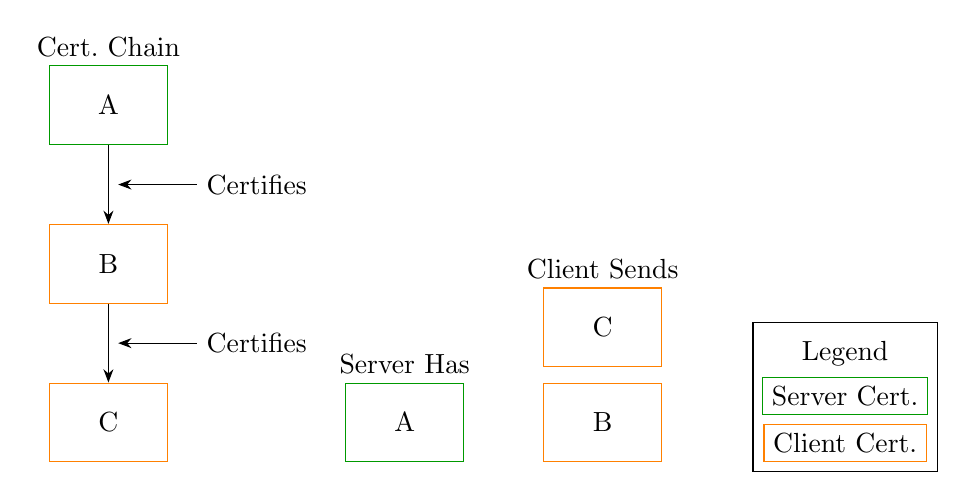
\begin{tikzpicture}
	% Styles.
	[s-cert/.style={rectangle,draw=green!60!black,minimum height=1cm,minimum width=1.5cm},
	c-cert/.style={rectangle,draw=orange,minimum height=1cm, minimum width=1.5cm}]
	% Certificate chain.
	\node (A) at (0, 0) [s-cert] {A};
	\node (B) [below=of A] [c-cert] {B};
	\node (C) [below=of B] [c-cert] {C};
	\draw[-Stealth] (A) -- (B)
		node[pos=0.5](a-cfies){};
	\node (a-cfies-txt) [right=of a-cfies] {Certifies};
	\draw[-Stealth] (a-cfies-txt) -- (a-cfies);
	\draw[-Stealth] (B) -- (C)
		node[pos=0.5](b-cfies){};
	\node (b-cfies-txt) [right=of b-cfies] {Certifies};
	\draw[-Stealth] (b-cfies-txt) -- (b-cfies);
	\node (txt) at (A) [above=0.5cm] {Cert.\ Chain};
	% Server certificates.
	\node (S-tmp) [right=of C] {};
	\node (S-A) [right=of S-tmp,s-cert] {A};
	\node (S-txt) at (S-A) [above=0.5cm] {Server Has};
	% Client certificates.
	\node (C-B) [right=of S-A,c-cert] {B};
	\node (C-C) at (C-B) [above=0.7cm,c-cert] {C};
	\node (C-txt) at (C-C) [above=0.5cm] {Client Sends};
	% Legend.
	\node (lanchor) at ($(current bounding box.south east) + (2, 0)$) {};
	\node (legend) at (lanchor) [above=1.1cm] {Legend};
	\node (l1) at (lanchor) [above=0.6cm,draw=green!60!black] {Server Cert.};
	\node (l2) at (lanchor) [above=0.0cm,draw=orange] {Client Cert.};
	\node [rectangle,draw,fit=(legend) (l1) (l2)] {};
\end{tikzpicture}
}
\end{makeimage}
\caption{Certificate chain where \texttt{A} is a trusted CA of the server and the client must send its certificate \texttt{C} followed by the intermediate certificate \texttt{B}.}
\end{figure}
\end{center}
After implementing a check for the entire peer certificate chain, my next problem was testing verification of the chain.  Consider the chain A -> B -> C, where A is trusted by the server and B and C are sent by the client.  I had been using OpenSSL's \texttt{s_client} command for testing, so the obvious approach was to place B and C into the file passed via the \texttt{-cert} argument; the first problem with this approach was that the certificates must be in a certain \emph{order}, specifically, the sender's certificate must come \emph{first}, followed by the certificate certifying the sender's certificate, and so on (see \htmladdnormallink{the RFC}{https://tools.ietf.org/html/rfc5246#section-7.4.2}).  In this case that meant sending C followed by B; specifying the certificates in the wrong order (B followed by C) was obvious, because \texttt{s_client} tried to use C's private key to verify B, which, of course, failed.  Putting them in the correct order, however, sent C while silently ignoring B.  After much gnashing of teeth, I decided to look into the source code, and, while combing through the parsing of the \texttt{-cert} option noticed an \emph{undocumented} (yes, not even in the \texttt{man} pages nor \texttt{-help} output) \texttt{-cert_chain} option.  After looking into it I ran the \texttt{s_client} command again with C sent via the \texttt{-cert} option and B sent via the \texttt{-cert_chain} option and was able to actually send a certificate chain to the server, and sanity was once again restored to my life.

\subsubsection{Testing}
Manually verifying changes is both a pain and error-prone, so I created a \htmladdnormallink{bash script}{https://github.com/clinew/inspircdtests/blob/master/ssl_strongcert.sh} in order to automatically test strong cert verification for InspIRCd on my system.  The tests check that the program runs without strong verification enabled, then turns verification on and checks that users can connect when their certificates use proper key type+sizes and algorithms, then checks that errors occur when invalid configuration options (such as non-existent algorithms) are specified, then finally checks that verification works correctly when the client passes a \emph{chain} of certificates.  It's not particularly exciting, but it gives peace of mind when rebasing on top of the latest stable release and when porting to newer versions of both OpenSSL and InspIRCd.

\subsection{Future Work}
After adding this feature I managed to find a series of functions that appeared as if they might do my heavy lifting for me.  The functions, found under the include directory as \texttt{ssl/ssl.h} were \texttt{SSL_set1_sigalgs_list()}, \texttt{SSL_set1_client_sigalgs_list()}, and a few similar variations.  Sadly, testing these show that they do not actually have the same functionality, although the signature algorithm list displayed after connecting via \texttt{s_client} was indeed different; presumably the signature algorithm is for session negation rather than peer certificate verification, but I am not yet sure as I have not yet Read The "Friendly" \strikeout{Manual} RFC.

The online man pages for the function also mentioned an \texttt{SSL_CONF} API, which might make option parsing easier; regardless, I didn't use it this time.


% Better Browsing With Firefox
\section{2018-01-17 Better Browsing With Firefox}
The Web is not what it once was, or at least not how I remember it.  It used to be like browsing a catalogue, with each link analogous to turning to a new page.  But the Web has transformed into something else entirely.  It is more like a \htmladdnormallink{two-way black mirror}{https://freedom-to-tinker.com/2017/11/15/no-boundaries-exfiltration-of-personal-data-by-session-replay-scripts} than a catalogue.  Every keystroke and mouse movement is logged and analyzed.  Users are tracked across unrelated websites by both visible widgets, invisible cookies, and more \htmladdnormallink{nefarious means}{https://en.wikipedia.org/wiki/Web_beacon}.  So-called "social media" sites analyze this data and censor their feeds in order to feed both themselves and their sponsors as much money as possible.  Basically, the Web has become a platform that consumes the user, rather than the user consuming the content of the Web.

Fortunately, there are ways to avoid being consumed by the Web and to create a more pleasant, catalogue-like browsing experience, but they are by no means obvious to the average person.  This blog will attempt to introduce the reader to some intermediate browsing techniques.  It assumes that the reader is already familiar with basic browser usage, and will then point out how, by installing a few add-ons, making a few configuration changes, and learning a few keystrokes, one's browsing experience can become both more controlled and more pleasant.  This requires work on the reader's part; it's not a give-me like most consumers desire, but tough shit, it's the world we currently live in.  This guide is divided into three sections, called "\htmladdnormallink{Power Levels}{https://www.youtube.com/watch?v=SiMHTK15Pik}", of increasing difficulty, with the first section requiring little to no work and having relatively little negative effect on one's browsing experience and a large positive effect, while the later sections require more work for often smaller gains.  Readers who are unsure of their skills should take a week or two in-between sections in order to familiarize themselves with any changes that they have made.

The Web browser of choice for this blog will be Firefox, because Firefox is \htmladdnormallink{Free Software}{https://www.gnu.org/philosophy/free-sw.en.html}.  Other common browsers, such as, but not limited to, Google Chrome, Safari, Microsoft Explorer, and Microsoft Edge are proprietary software and, therefore, \htmladdnormallink{considered harmful}{https://www.gnu.org/proprietary/proprietary.en.html}.  Make no mistake, Firefox has its flaws and its parent company, Mozilla Corporation, has made some \htmladdnormallink{questionable decisions}{http://lunduke.com/2017/12/17/mozilla-is-not-trustworthy}, but it's currently the best of the Free and featureful browsers to use.

\subsection{Power Level One}
\begin{figure}
\includegraphics[scale=0.5]{files/blog/2018_01_17_better_browsing_with_firefox/2018_01_17_ublockorigin_icon.png}
\caption{The uBlock Origin icon.}
\end{figure}
The first thing to do is to install the "uBlock Origin" add-on from the \htmladdnormallink{Mozilla Add-Ons}{https://addons.mozilla.org/en-US/firefox} webpage in order to block advertisements.  That's it.  Once it's installed, most advertisements will cease to be, and browsers without an ad-blocker will seem like a headache, because they are.  Sadly, a few sites will detect that one is using an ad-blocker and refuse to display any content, in which case you can disable the add-on \textit{for that site alone} by clicking on the uBlock Origin icon, then clicking the big ol' power-button icon in the drop-down menu that appears, but do note that most sites that are this ad-infested tend to suck and aren't worth reading anyways, in the same way that the trashiest magazines at the grocery checkout always have more advertisements than content in them.  Go figure.  Another icon worth noting is the little, Harry Potter-esque lightning icon, called the \textit{element zapper}.  Clicking on that icon will allow one to enter an element-zapper mode where one can select an element on the site for removal from their browser by clicking on it.  Hold \texttt{Shift} while clicking in order to continue removing elements, and press \texttt{Esc} to return to normal browsing mode.  Removals are not permanent, thus refreshing the page will reload any removed elements.  uBlock Origin can do this in part because it's actually a \textit{generic blocker} and not just an ad-blocker, but for now simply know that it's configured to block ads.

It's worth noting that there are other ad-blockers.  "AdBlock Plus" (ABP) is noteworthy for having been the de facto standard for a while before falling out of favor by many due to an \htmladdnormallink{"acceptable ads"}{https://adblockplus.org/acceptable-ads} campaign, in which certain, "unobtrusive" advertisements are not blocked by default and a portion of the revenue generated by the advertisements in sent to the ABP developers.  The AdBlock Plus add-on also tends to take up far more memory than uBlock Origin, which gave me issues on my low-memory machines, thus I prefer uBlock Origin for that reason alone.  There's also "uBlock", which was originally developed by the author of uBlock Origin, but apparently there were some issues and now the original author is working on uBlock Origin and that's what I've decided to use.  Feel free to check out the other one if you are so inclined.

\begin{figure}
\includegraphics[scale=0.5]{files/blog/2018_01_17_better_browsing_with_firefox/2018_01_17_httpseverywhere_icon.png}
\caption{The HTTPS Everywhere icon.}
\end{figure}
The next thing to do is to install the "HTTPS Everywhere" add-on developed by the \htmladdnormallink{Electronic Frontier Foundation}{https://www.eff.org/} (EFF).  A brief explanation is in order: HyperText Transfer Protocol (HTTP) is the protocol used for the Web, and HTTP\textbf{S} is, roughly speaking, the \textit{\textbf{S}ecure} version of that protocol.  HTTPS is useful because it's the reason \htmladdnormallink{crackers}{https://stallman.org/articles/on-hacking.html} cannot easily break into your bank account or use your credit card when you are browsing the web.  Many sites offer both secured and unsecured versions of their webpages but configure their websites such that users must explicitly request the secure version of the website by prefixing the address with \texttt{https://}, which is a giant pain in the ass.  HTTPS Everywhere fixes this problem by automatically \textit{rewriting} (a.k.a. "changing") any HTTP addresses to their secure, HTTPS variants, no user intervention required.  This is done through a database of sites that comes with the program; the database knows how to rewrite addresses for different sites.  Although a few, very obscure sites may not have their addresses rewritten, the vast majority will.

Lastly, it is worth learning one mouse click technique and a few simple key-commands.  Most mice have a scroll wheel in the middle, and that scroll wheel can be pressed in order to generate a "middle-mouse button click", or "middle-click" for short.  Middle-clicking a link will open said link in a new tab.  This is far faster than going through the tedious process of right-clicking the link and then selecting "Open in New Tab" from the drop-down menu.  It's a serious time-saver.  Use it.  The middle-mouse click can also be used to close a tab by clicking on the tab itself.  Ever accidentally close a tab and then realized that it shouldn't have been closed?  Type \texttt{Ctrl-Shift-T} to bring it back!  Continue typing the command in order to bring back tabs in the order in which they were closed.  Finally, \texttt{Ctrl-F} can be used to \textit{Find} text within a webpage.  Just in case one wasn't aware.

That's it for this first section.  One's browsing experience should now be ad-free, far more secure, and hopefully a little bit smoother with those middle-clicks.  There probably won't be any disruption in one's browsing experience, but take some time to get used to it before proceeding onto the next section.

\subsection{Power Level Two}
This section will impact one's browsing experience far more than the previous section.  This section also plays the largest part in disabling the two-way mirror "functionality" of the Web.  This involves changing a few configuration options, installing a new add-on, and finally learning a few keyboard shortcuts.

Begin by making some configuration changes to Firefox that will cause each \textit{session} to be independent of the others.  In other words, each time Firefox is closed and opened it will be as if no websites had been visited during the previous time Firefox was open, even if they were, as if Firefox had just been installed, except, of course, the add-ons, bookmarks, and other user-defined settings will remain.  I could try and describe the bloody icons that lead to the \texttt{Preferences} menu, but it'll be easier if I tell you to simply type \texttt{F10} to open the old-style text-based menu and then navigate to \texttt{Edit -> Preferences}.  From there, click on the tab labeled \texttt{Privacy}, then find the section labelled \texttt{History} and change the corresponding drop-down to \texttt{Never remember history}.  Likewise, next find the section labelled \texttt{Location Bar} and uncheck all of the boxes.  Lastly, click on the tab labelled \texttt{Advanced}, then another tab labelled \texttt{Network} and finally the section labelled \texttt{Cached Web Content} and check the \texttt{Override automatic cache management} checkbox and then set the specified value to \texttt{0 MB}.  That should make each browsing session far more independent and thus make tracking more difficult, but it will be noticeable as many sites that require a login will no longer "remember" one's username and one will thus have to type it in again.

\begin{figure}
\includegraphics[scale=0.5]{files/blog/2018_01_17_better_browsing_with_firefox/2018_01_17_noscript_icon.png}
\caption{The NoScript icon.}
\end{figure}
Next comes the biggest change: installing the "NoScript" add-on.  This add-on is what allows one to selectively enable and disable JavaScript.  Unlike plain HTML, JavaScript is actually code that is sent by the web server and run on the user's computer.  This code is what allows the browser to track the user's mouse movements, keystrokes, and gather various information about the user's system.  The fact that browsers run arbitrary JavaScript code on the user's computer is a large part of what turns the Web from a catalogue into a two-way mirror (confusingly enough, JavaScript has no relationship to the Java programming language).  What NoScript does is to give one some control over what JavaScript is run on their computer.  The default is to block all JavaScript, which will cause many sites to break, but scripts can be allowed on a per-site basis by clicking the NoScript icon and then selecting \texttt{Temporarily allow from <address>} from the drop-down menu where \texttt{<address>} is the name of the site that the JavaScript is loaded from, and when the drop-down menu is closed the site will automatically reload with the selected scripts enabled.  Note that most sites load JavaScript from multiple sources, thus the \texttt{Temporarily allow all this page} option can come in handy when one wants to load all scripts on the site, but note, however, that some scripts will then drag in other scripts, and thus for certain sites one will have to "allow all" for the site multiple times.  Note that any allowances made will apply to \textit{all} tabs that one has opened, not just the current tab.  When one no longer wishes to allow scripts, clicking the icon again and selecting the \texttt{Revoke temporary permissions} will disable all scripts and refresh the sites whose scripts were revoked.  It's actually quite simple once one gets the hang of it.

After using NoScript for a while one will inevitably notice that certain addresses come up again and again.  Most notorious in my opinion is \texttt{google-analytics.com}.  Since I have absolutely no desire to be analyzed by The Googlaug ever, I banished the script permanently by clicking the NoScript icon, then selecting \texttt{Untrusted -> Mark google-analytics.com as untrusted}, thus removing it from the drop-down menu.  Good riddance.  The drop-down menu can be customized by selecting \texttt{Options} and then the \texttt{Appearance} tab and toggling the various boxes.  It can be useful to uncheck the \texttt{Allow [...]} and \texttt{Allow all this page} boxes if one does not wish to even accidentally give some scripts permanent permission.

Now, NoScript actually does a little more than just block JavaScript, it also protects against a few types of Web-based attacks by blocking \htmladdnormallink{Cross-Site Scripting (XSS)}{https://en.wikipedia.org/wiki/Cross-site_scripting} and implementing \htmladdnormallink{Application Boundary Enforcer (ABE)}{https://noscript.net/abe/}.  Although these are generally considered a Good Thing (TM), they occasionally cause problems with crappy Web portals, for example, at one's local library where one is required to agree to a Terms of Service (ToS), and need to be disabled.  ABE can usually be worked around by choosing the "Unsafe Reload" option after it has been triggered, but both can be disabled by opening the options window, selecting the \texttt{Advanced} tab and then selecting either the \texttt{XSS} or \texttt{ABE} tab and turning the offending feature off.  With that one should now have some basic control over the JavaScript run on one's own computer.

A few more useful key-commands are now in order.  First, \texttt{Ctrl-L} and \texttt{Ctrl-J} move the cursor to the Location and Search Bar, respectively.  For tab-management, \texttt{Ctrl-T} opens a new tab, \texttt{Ctrl-W} closes the current tab, and \texttt{Ctrl-Q} quits the browser program; because the \texttt{Q} key is right next to the \texttt{W} key, it's a good idea to keep the "Warn me when I attempt to close multiple tabs" checkbox enabled.  Lastly, use \texttt{Ctrl-PgUp} (Page Up) and \texttt{Ctrl-PgDn} (Page Down) in order to move to the previous and subsequent tab, respectively.

Thus ends the second section.  Each browser session should now be more independent and two-way mirror functionality will be disabled by default.  These are both rather large changes to make, but they offer significant privacy and security advantages, so the added difficulty is often worthwhile.  Make sure to become comfortable with these changes before moving onto the next section.

\subsection{Power Level Three}
As explained in the first section, uBlock Origin is actually a \textit{generic blocker}, meaning that it can block more than just ads.  Ad-blocking is actually done via a \textit{filter list} which is provided by a third party, and there exist more than just ad-filter lists, for example, filter lists to block embedded tracking widgets from sites like Farcebook.  In order to view the filter lists, click on the uBlock Origin icon and then click on the icon that looks like, uh, well, three lines with some kind of slider-thingies on it (damn icons) in order to open the "dashboard", and then click on the "3rd party filters" tab in order to view a default list of filters.  Learn more about each filter by clicking on the house icon in order to be directed to a webpage containing information about the filter, and enable/disable filters by checking/unchecking their respective boxes.  I like "Fanboy's Social Blocking List" myself.  One can also manually update their lists by clicking the obvious "Update Now" button while on this tab.

Filter lists are nice for most uses, but sometimes one needs custom filters on a site; this can be done by clicking "I am an advanced user" in the dashboard's "Settings" tab and thus enabling \textit{dynamic filtering}; make sure to read the corresponding documentation under \htmladdnormallink{required reading}{https://github.com/gorhill/uBlock/wiki/Advanced-user-features} before trying to apply any dynamic filters; they are not covered here because the existing documentation is better than what I would write.  Note that after enabling dynamic filtering it's interesting enough to simply click on the uBlock Origin icon after loading a site and seeing which sites one's browser has connected to.  In a similar vein to the zapper icon (in the menu that appears after clicking the uBlock Origin icon), the eye-dropper, or \textit{element picker}, helps create custom filter rules rather than simply removing an element until the page is reloaded, but be careful about the filters it creates unless one wants to filter more than intended.  Adding custom filters in more of an art than a science, but it provides incredible control over which services get to track one's virtual movement across the Web.

When customizing Firefox, one might be tempted to naively believe that, after clicking on the gear icon and perusing all sections and tabs and setting things up as one desires that they're finished with all possible non-add-on-based customizations.  However, Firefox, in fact, actually has a, well, it's not exactly \textbf{hidden}, but \textbf{unadvertised}, perhaps, customization menu that can be reached by typing \texttt{about:config} into the address bar (then hitting \texttt{Enter}, obviously).  This page consists of a list of \textit{preferences} with a \textit{type} and \textit{value} and whose values can be customized by the user.  A full discussion of all preferences in this menu would likely require an entire encyclopedia, so only a few noteworthy preferences are mentioned here.  First off is the \texttt{UserAgent}, which is a string containing various client metadata such as operating system, browser vendor, browser version, \&c, and which is sent to the web server when the connection is first established so that the web server can serve up client-specific \htmladdnormallink{hacks}{https://en.wikipedia.org/wiki/Hack_(computer_science)}, \htmladdnormallink{nevermind that the whole damn point of the web was to be platform-independent}{http://www.catb.org/~esr/html-hell.html}.  One can view their \texttt{UserAgent} by navigating to \texttt{about:} in the address bar, and one can customize it in the \texttt{about:config} menu by right-clicking then selecting \texttt{New -> String} and then giving the preference name \texttt{general.useragent.override} and then providing whatever value one wants; check \texttt{about:config} to confirm.  Note that poorly-designed sites will break if they can't supply custom browser-specific hacks, for example, this is what Googlaug Voice looks like with the classy \texttt{UserAgent} of "Fuck JavaScript":
\begin{figure}
\includegraphics[scale=0.33]{files/blog/2018_01_17_better_browsing_with_firefox/2018_01_17_googlaug_voice.png}
\caption{These modern interfaces really know how to cut down on bloat!}
\end{figure}
Note that using a custom \texttt{UserAgent} is \htmladdnormallink{probably less anonymous than one might think}{https://panopticlick.eff.org/}.

A few other noteworthy preferences are \texttt{javascript.options.asmjs} which allows JavaScript to run native code on one's computer and will probably cause some security nightmare within the next decade or two (set it to \texttt{false} now).  One may also wish to set \texttt{webgl.disabled} to \texttt{true}, although NoScript already forbids WebGL by default.  Due to \htmladdnormallink{recent events}{https://sircmpwn.github.io/2017/12/16/Firefox-is-on-a-slippery-slope.html} one will probably want to set \texttt{experiments.enabled} to \texttt{false}.  Note that while one might be tempted to set \texttt{javascript.enabled} to \texttt{false}, JavaScript is actually used internally by the browser and add-ons, and thus disabling it here actually causes add-ons to not function properly, relying on NoScript is recommended instead.

This section has been rather open-ended, because customizations at this point have become, well, highly-customized.  Nonetheless, one should now have an idea of how to go about blocking content on websites they visit and performing deep configuration of Firefox.

\subsection{Conclusion}
That's it for this guide.  Hopefully one's browser experience is now both cleaner and more controlled than it had been before.  While it may have been a large amount of information to take in, please understand that there is still much more to be learned about the Web and its oftentimes questionable behaviour, and please note that none of these techniques are meant to make one anonymous, as that is the aim of other projects such as \htmladdnormallink{Tor}{https://torproject.org} and \htmladdnormallink{TAILS}{https://tails.boum.org}.  Regardless, one who has followed this guide should now be able to begin taking back control of their Web experience.  Good luck.


% 4.9-4.14 Kernel Upgrade USB Woes
\section{2018-01-08 4.9-4.14 Kernel Upgrade USB Woes}
Given the recent concerns over the Meltdown/Spectre vulnerabilities and the release of \htmladdnormallink{new stable kernels}{https://lwn.net/Articles/743246/}, I figured that now would be a good time to do a quick kernel upgrade.  As you have probably surmised by the very existence of this blog post, the "quick" upgrade turned into a bit of a headache.

Rather than using another 4.9 kernel with a backported mitigation, I decided that now would be a good time to upgrade to the newer 4.14 kernel.  The usual process went smoothly: downloading, verifying the signature, updating the configuration, compiling, and finally booting.  Except there was one little problem after booting: I couldn't enter my passphrase from my keyboard in order to decrypt the root filesystem.  Huh?  The keyboard, which is a USB keyboard, had worked before the BIOS hand-off, and it still had power, but no key-presses, even SysRq keys, had any effect.  Other than that, the kernel seemed perfectly fine, no backtraces or nasty error messages being spewed out.

Okay, well, at this point I was rather dumbfounded.  Nothing in the output of \texttt{make oldconfig} that I could recall suggested something that would break my USB keyboard, and the only thing that I really cared about in this upgrade was the new Kernel Page-Table Isolation (KPTI) feature, but maybe this was some weird bug with it and my \texttt{initramfs}, so I tried disabling it, recompiling the kernel, and booting the recompiled kernel.  Still broken.  So, at least the security feature that I'd upgraded for wasn't the source of my woes, but that didn't solve my problem.  At this point it also occurred to me that no messages for the attached USB storage device were showing up, either, so this was some kind of USB problem.  Perhaps the problem was specific to the front ports?  I decided to try the back ports, which are attached directly to the motherboard, and did not have any luck there, either.

Perhaps I'd missed something when updating the configuration, so I saved my new configuration and re-ran \texttt{make oldconfig} on a copy of the old configuration and noted any options that \textit{might possibly} be affecting my USB devices.  A few possibilities emerged, including \texttt{X86_MCELOG_LEGACY} (the \texttt{initramfs} is rather old), \texttt{SERIAL_DEV_BUS} (are the USB devices connected to the motherboard via serial?), \texttt{RC_CORE} (uhh do I have video capture?), \texttt{USB_PCI}, and \texttt{USB_HUB_USB251XB}.  The latter two options seemed the most suspicious.  The help information for \texttt{USB_PCI} reads:
\begin{quote}
\begin{verbatim}
	A lot of embeded system SOC (e.g. freescale T2080) have both
	PCI and USB modules. But USB module is controlled by registers
	directly, it have no relationship with PCI module.

	When say N here it will not build PCI related code in USB driver.
\end{verbatim}
\end{quote}
English is obviously not their native language, but code isn't mine, so fair's fair.  It sounds like there's PCI code in the USB module for\ldots~no reason?  Well, I don't have any USB hubs connected via PCI add-on cards, so this should be safe left disabled.  Regarding \texttt{USB_HUB_USB251XB}, perhaps some hub-specific code got moved into a separate option and I happen to be using that hub.

No clear winner emerged, so I opened the case in order to examine how the USB ports were connected and what hubs were in use:
\begin{figure}
\includegraphics[scale=0.5]{files/blog/2018_01_08_kernel_upgrade_usb_woes/motherboard.png}
\caption{"Can you find the PCI USB on this motherboard?  Neither could we."}
\end{figure}
The back ports are directly connected to the motherboard, and the front ports are connected by some\ldots~thing to the motherboard.  I have no idea how components on the motherboard are interconnected (I2C?, serial?, gnomes?), but the USB hubs are certainly not connected via PCI cards, and I couldn't find any "USB251XB" markings on or around the hubs, not that I could particularly make out the small, cryptic writings on the board anyhow.  After blowing out some dust and a couple of sneezes later I went back to scratching my head.  Perhaps \texttt{make oldconfig} didn't tell me everything.  I decided to run a \texttt{diff -u} in-between the old and new configuration, and one line in particular caught my eye:
\begin{quote}
\begin{verbatim}
	-CONFIG_USB_UHCI_HCD=y
\end{verbatim}
\end{quote}
Now I cannot for the life of me remember what each of the \texttt{_HCI} USB configurations refer to what vendor/version combination, but this seemed like a \textit{very} strange omission.  Going into \texttt{menuconfig} and searching for the option was even more telling:
\begin{quote}
\begin{verbatim}
	Prompt: UHCI HCD (most Intel and VIA) support
\end{verbatim}
\end{quote}
"most Intel", eh?  So why was this option magically unselected?
\begin{quote}
\begin{verbatim}
	Depends on: USB_SUPPORT [=y] && USB [=y] && (USB_PCI [=n] || USB_UHCI_SUPPORT_NON_PCI_HC [=n])
\end{verbatim}
\end{quote}
Right, so, disabling the new \texttt{USB_PCI} option will \textit{silently} disable \texttt{USB_UHCI_HCD} \textit{even if it was already selected}.  Could this be my problem?  I enabled both \texttt{USB_PCI} and \texttt{USB_UHCI_HCD}, recompiled, booted, and, lo and behold, my USB devices started working again.

So much for a "quick" upgrade.  While I'm glad to have things working again, it would have been nice if the \texttt{USB_PCI} help had clarified that whether or not PCI code is needed in the USB module \textit{depends on the system}, because the current wording suggests that it \textit{never} has any relationship to the PCI module ("it have no relationship with PCI module", said without qualifications).  Something along the lines of, "in these embedded systems, the USB module has no relationship to the PCI module" would have been better.  It also would have been nice if the \texttt{USB_UHCI_HCD} options wasn't silently disabled, but that may be a limitation of the Kconfig language; I don't know.  At least things are working again\ldots~at least until the other cache vulnerabilities start being exploited \texttt{;)}.


% Booting BeagleBone Black With an Initramfs
\section{2017-10-05 Booting BeagleBone Black With an Initramfs}
\begin{center}
\begin{figure}
\begin{makeimage}
\newcommand{\fn}[1]{\hspace*{1ex}\texttt{#1}}
\fbox{
\begin{tabular}{l l}
Before: & After: \\
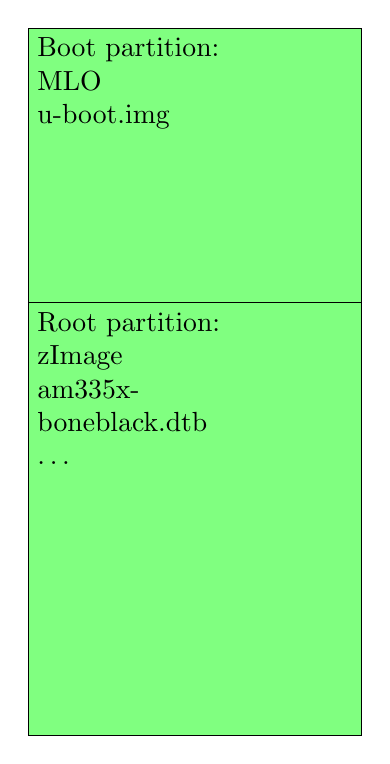
\begin{tikzpicture}
	\node at (0, 0) [rectangle split,rectangle split parts=2,rectangle split part fill={green!50, green!50},align=left,draw,text width=4cm]
		{\rule[-3cm]{0cm}{3cm}\parbox[t]{3cm}{Boot partition: \\ \fn{MLO} \\ \fn{u-boot.img}}
		\nodepart{two} \rule[-5cm]{0cm}{5cm}\parbox[t]{3cm}{Root partition: \\ \fn{zImage} \\ \fn{am335x-boneblack.dtb} \\ \fn{\ldots}}};
\end{tikzpicture}
&
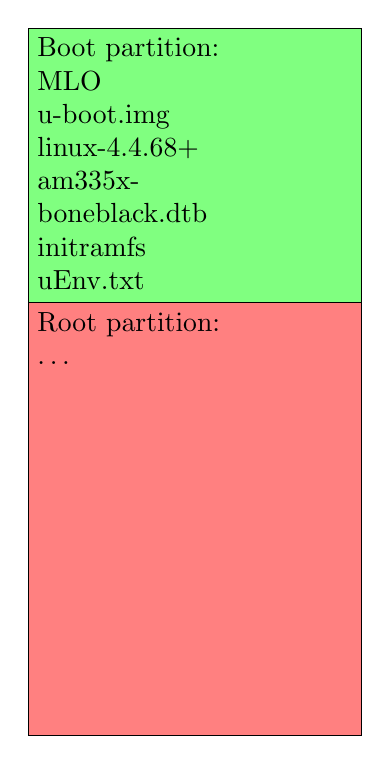
\begin{tikzpicture}
	\node at (0, 0) [rectangle split,rectangle split parts=2,rectangle split part fill={green!50, red!50},align=left,draw,text width=4cm]
		{\rule[-3cm]{0cm}{3cm}\parbox[t]{3cm}{Boot partition: \\ \fn{MLO} \\ \fn{u-boot.img} \\ \fn{linux-4.4.68+} \\ \fn{am335x-boneblack.dtb} \\ \fn{initramfs} \\ \fn{uEnv.txt}}
		\nodepart{two} \rule[-5cm]{0cm}{5cm}\parbox[t]{3cm}{Root partition: \\ \fn{\ldots}}};
\end{tikzpicture}
\end{tabular}
\begin{tabular}{c l}
\multicolumn{2}{c}{\textbf{Legend}} \\

\begin{tikzpicture}
	\node at (0, 0) [fill=green!50,draw] {};
\end{tikzpicture} & Unencrypted \\

\begin{tikzpicture}
	\node at (0, 0) [fill=red!50,draw] {};
\end{tikzpicture} & Encrypted
\end{tabular}
}
\end{makeimage}
\caption{Visualization of the SD Card before and after modifications.  Contents are not to scale.}
\end{figure}
\end{center}

The instructions for installing Gentoo on my BeagleBone Black (BBB)\htmladdnormallink{[1]}{https://wiki.gentoo.org/wiki/BeagleBone_Black} gave me a working OS, but one without the root partition encrypted.  Unencrypted OSes make me sad, but an encrypted root partition means using an \texttt{initramfs}; to make matters more complicated, the kernel and device tree are on the root partition, but they need to be on the boot partition (because the root partition will be encrypted).  This blog will explain how I was able to make these changes; it will not cover creating an \texttt{initramfs} nor creating an encrypted root partition using LUKS and \texttt{cryptsetup}.

\subsection{Das U-Boot}
Das U-Boot, colloquially known simply as "U-Boot", is roughly analogous to the BIOS and/or UEFI portion of normal desktop towers.  Like desktops, the boot process can be interrupted and the user taken to a configuration interface by typing a certain key early on in the boot process.  For the BBB, this can be done by pressing the 'Space' button, which takes the user to a Command-Line Interface (CLI); from here, \texttt{help} may be run in order to provide a list of commands or to print usage information for a specific command.  One of the most useful commands to run is \texttt{printenv}, which will list all of the environment variables; these variable are important because their values can be either simple values or an entire script.  It is these variables that must be modified in order to load and boot an \texttt{initramfs}, kernel, and device tree file from the boot partition.

While one can modify the environment variables before each boot, this is extremely tedious.  Thankfully, U-Boot allows one to define a \texttt{uEnv.txt} file in the boot partition that will be read in before the boot process is completed and which will set the environment variables as specified in the file.  Thus one can simply write this file rather than constantly modify the environment variables at each boot.

\subsection{uEnv.txt}
This section will explain what variables I added/modified and why I modified them.  Though they are all crammed together in the actual file, for conceptual purposes I will divide them into three categories: filename definitions, load scripts, and boot scripts.

The first of the sections, filename definitions, is straightforward enough:
\begin{quote}
\begin{verbatim}
	# BEFORE
	bootfile=zImage
	# AFTER
	bootfile=linux-4.4.68+
	rdfile=initramfs
\end{verbatim}
\end{quote}
Although changing the name from \texttt{zImage} to \texttt{linux-4.4.68+} isn't strictly necessary, I prefer to have my kernels include their version in the name as it makes booting, upgrading, and dealing with regressions easier.  The \texttt{rdfile} variable is added for consistency with the existence of the \texttt{bootfile} variable, and is used later.  Note that the same \texttt{initramfs} can often be used across multiple kernel versions.

The second section, load scripts, consists of the series of commands used to load the kernel, initramfs, and device tree into memory:
\begin{quote}
\begin{verbatim}
	# BEFORE
	loadimage=load ${devtype} ${bootpart} ${loadaddr} ${bootdir}/${bootfile}
	loadfdt=load ${devtype} ${bootpart} ${fdtaddr} ${bootdir}/${fdtfile}
	loadramdisk=load mmc ${mmcdev} ${rdaddr} ramdisk.gz
	# AFTER
	loadimage=fatload mmc ${mmcdev} ${loadaddr} ${bootfile}
	loadfdt=fatload mmc ${mmcdev} ${fdtaddr} ${fdtfile}
	loadramdisk=fatload mmc ${mmcdev} ${rdaddr} ${rdfile}
\end{verbatim}
\end{quote}
A few things are worth noting here.  First is that I ignored the \texttt{devtype} and \texttt{bootpart} variables and just loaded the kernel (\texttt{loadimage}), device tree (\texttt{loadfdt}), and initramfs (\texttt{loadramdisk}) directly from the MMC (SD Card), since that is what I wanted; this worked on my SD Card, but may be fragile on other configurations, use at your own risk!  Second, there is already an instruction for loading a ramdisk which, from a cursory glance of other environment variables, appears to be associated with boot code for a live OS rather than an \texttt{initramfs} for booting; since I currently am not interested in nor know how to use this functionality, it appears safe to modify.  Last, I removed the \texttt{bootdir} prefix for the kernel and device tree filepaths, since I'm simply going to place them at the root directory of the boot partition.

The last section, boot scripts, is the most complicated section, because it contains the commands and logic needed to actually boot the system:
\begin{quote}
\begin{verbatim}
	# BEFORE
	args_mmc=run finduuid;setenv bootargs console=${console} ${optargs} root=PARTUUID=${uuid} rw rootfstype=${mmcrootfstype}
	mmcloados=run args_mmc; if test ${boot_fdt} = yes || test ${boot_fdt} = try; then if run loadfdt; then bootz ${loadaddr} - ${fdtaddr}; else if test ${boot_fdt} = try; then bootz; else echo WARN: Cannot load the DT; fi; fi; else bootz; fi;
	# AFTER
	args_mmc=run finduuid;setenv bootargs console=${console} ${optargs} root=/dev/mapper/mmcblk0p2 initrd=initramfs rw rootfstype=${mmcrootfstype}
	mmcloados=run args_mmc; run loadramdisk; if test ${boot_fdt} = yes || test ${boot_fdt} = try; then if run loadfdt; then bootz ${loadaddr} ${rdaddr} ${fdtaddr}; else if test ${boot_fdt} = try; then bootz; else echo WARN: Cannot load the DT; fi; fi; else bootz; fi;
\end{verbatim}
\end{quote}
While the commands may appear relatively complex, the modifications are actually pretty simple.  For \texttt{args_mmc}, the \texttt{root=PARTUUID=\${uuid}} had to be changed to the mapping set up by the encryption scripts, in my case to \texttt{root=/dev/mapper/mmcblk0p2}; the argument \texttt{initrd=initramfs} was also added to let the kernel know about the \texttt{initramfs} file (but may not strictly be necessary in this context).  Two modifications were made to \texttt{mmcloados}: the first was to load the initramfs by calling \texttt{run loadramdisk;}, the second was to change the \texttt{bootz} command to contain the address of the \texttt{initramfs} to load (\texttt{rdaddr}) rather than not loading one (\texttt{-}).

Thus with each of these modifications I was able to boot with an encrypted root partition.  Hopefully you will have the same luck, and don't forget to copy your files from the root partition to the boot partition!


% Adding Certificate Revocation Lists (CRLs) to an Existing OpenSSL Implementation.
\section{2017-09-22 Adding Certificate Revocation Lists (CRLs) to an Existing OpenSSL Implementation}
I recently took it upon myself to add Certificate Revocation List (CRL) functionality to an SSL-enabled program (\htmladdnormallink{InspIRCd}{https://github.com/inspircd/inspircd/pull/1370}).  This blog details both the code that I used and some unexpected functionality regarding how CRLs behave.  Hopefully this blog will prove useful to someone else who needs to tread this path.

\subsection{Code Itself}
The code itself is actually quite simple, consisting of two basic steps: loading the CRL files and then enabling CRL checking.  In order to load the CRL files, begin by getting the \texttt{X509_STORE *} from the \texttt{SSL_CTX *} by calling \texttt{SSL_CTX_get_cert_store(3)}, then load the CRL files into the \texttt{X509_STORE *} by calling \texttt{X509_STORE_load_locations()} with the specified CRL file and path locations.  The definition of the functions can be found in \texttt{openssl/x509_vfy.h} in your system's include file directory.  The code looks something like:
\begin{quote}
\begin{verbatim}
	SSL_CTX *ctx = sslctx; // Defined elsewhere.
	X509_STORE *store;
	char *crlfile = "/path/to/single/file.pem";
	char *crlpath = "/path/to/entire/directory";

	if (!(store = SSL_CTX_get_cert_store(ctx))) {
		fprintf(stderr, "No cert store found\n");
		return -1;
	}
	if (!X509_STORE_load_locations(store, crlfile, crlpath)) {
		fprintf(stderr, "Unable to load CRL files\n");
		return -1;
	}
\end{verbatim}
\end{quote}
This will load the CRL files, but will not enable CRL checking; this has to be done by setting a flag value in the \texttt{X509_STORE *}.  There at least two possible options: one is to check only the leaf certificate, the other is to check all certificates in the chain.  The former option can be accomplished by setting only \texttt{X509_V_FLAG_CRL_CHECK} while the latter can be accomplished by setting two flags \texttt{X509_V_FLAG_CRL_CHECK | X509_V_FLAG_CRL_CHECK_ALL}.  The latter option (the entire chain) is almost certainly what you want.
\begin{quote}
\begin{verbatim}
	char* crlmode; // Defined elsewhere.
	int crlflags;

	if (!strcmp(crlmode, "chain")) {
		crlflags = X509_V_FLAG_CRL_CHECK | X509_V_FLAG_CRL_CHECK_ALL;
	} else if (!strcmp(crlmode, "leaf")) {
		crlflags = X509_V_FLAG_CRL_CHECK;
	} else {
		fprintf(stderr, "Unknown flag mode '%s'\n", crlmode);
		return -1;
	}
	if (X509_STORE_set_flags(store, crlflags) != 1) {
		fprintf(stderr, "Unable to set flags\n");
		return -1;
	}
\end{verbatim}
\end{quote}
\ldots and that's it!  CRLs should now be enabled for your program.  However, do not rest easily just yet, as CRLs offer several pitfalls for the unwary, as detailed below.

\subsection{Missing CRL Files}
Consider\label{2017-09-22-missing-crls} the following, simple certificate chain:
\begin{center}
\begin{figure}
\begin{makeimage}
\fbox{
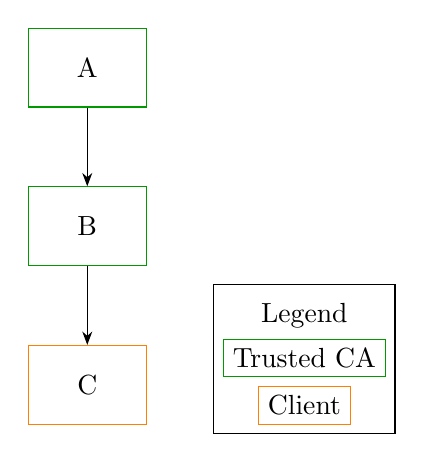
\begin{tikzpicture}
	% Styles.
	[ca/.style={rectangle,draw=green!60!black,minimum height=1cm,minimum width=1.5cm},
	leaf/.style={rectangle,draw=orange,minimum height=1cm, minimum width=1.5cm}]
	% Certificates.
	\node (A) at (0, 0) [ca] {A};
	\node (B) [below=of A] [ca] {B};
	\node (C) [below=of B] [leaf] {C};
	\draw[-Stealth] (A) -- (B);
	\draw[-Stealth] (B) -- (C);
	% Legend.
	\node (lanchor) at ($(current bounding box.south east) + (2, 0)$) {};
	\node (legend) at (lanchor) [above=1.1cm] {Legend};
	\node (l1) at (lanchor) [above=0.6cm,draw=green!60!black] {Trusted CA};
	\node (l2) at (lanchor) [above=0.0cm,draw=orange] {Client};
	\node [rectangle,draw,fit=(legend) (l1) (l2)] {};
\end{tikzpicture}
}
\end{makeimage}
\caption{Simple certificate chain, where A and B are CAs and C is the client.}
\end{figure}
\end{center}
The server trusts Certificate Authorities (CAs) A and B to issue valid certificates, thus C's certificate will be accepted.  Without CRLs this scenario will work as expected, C will be able to connect to the server without a problem.  Now, assume that the server enables CRLs, generates a CRL for A, and then configures itself to use A's CRL; a CRL for B is not generated as B has not revoked any certificate and thus there doesn't \emph{seem} to be any need to generate a CRL for B.  As you can probably guess by now, C will not be able to connect in this scenario, because the default CRL-checking method requires \emph{every} CA in the chain to have a CRL file loaded, thus C cannot connect unless both A \emph{and} B generate CRL files, \emph{even if they have no revoked certificates}.
\begin{center}
\begin{figure}
\begin{makeimage}
\fbox{
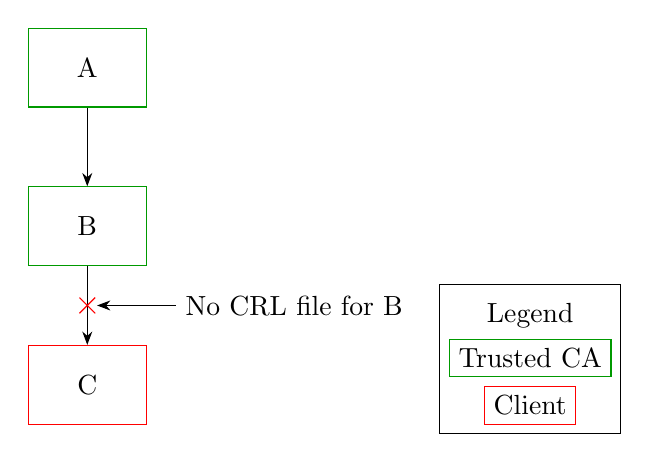
\begin{tikzpicture}
	% Styles.
	[ca/.style={rectangle,draw=green!60!black,minimum height=1cm,minimum width=1.5cm},
	leaf/.style={rectangle,draw=red,minimum height=1cm, minimum width=1.5cm},
	x/.pic={
		\draw[-] (-1mm,1mm) -- (1mm,-1mm);
		\draw[-] (-1mm,-1mm) -- (1mm,1mm);
	}]
	% Certificates.
	\node (A) at (0, 0) [ca] {A};
	\node (B) [below=of A] [ca] {B};
	\node (C) [below=of B] [leaf] {C};
	\draw[-Stealth] (A) -- (B);
	\draw[-Stealth] (B) -- (C)
		node[pos=0.5](fail){}
		pic [pos=0.5,red] {x};
	\node (error) [right=of fail] {No CRL file for B};
	\draw[-Stealth] (error) -- (fail);
	% Legend.
	\node (lanchor) at ($(current bounding box.south east) + (1.5, 0)$) {};
	\node (legend) at (lanchor) [above=1.1cm] {Legend};
	\node (l1) at (lanchor) [above=0.6cm,draw=green!60!black] {Trusted CA};
	\node (l2) at (lanchor) [above=0.0cm,draw=red] {Client};
	\node [rectangle,draw,fit=(legend) (l1) (l2)] {};
\end{tikzpicture}
}
\end{makeimage}
\caption{Each CA is required to have a CRL file.}
\end{figure}
\end{center}

The consequence of this is that enabling CRL-checking requires gathering CRL files, a task that is likely non-trivial.  The alternative is to override OpenSSL's verify callback by defining your own verify function and then telling OpenSSL to use said function with \texttt{X509_STORE_set_verify_cb(3)}.  I, however, do not intend to touch that with a 10-foot pole.

\subsection{Using a CRL Path}
Suppose that you wish to use a directory to store CRL files separately for each CA (instead of one big CRL file), then have OpenSSL load in each CRL file from this directory.  An obvious benefit of this approach is that it allows you to create a separate CRL file for each CA; using the certificate chain from the previous section, this would mean a directory containing both \texttt{crl/a.pem} and \texttt{crl/b.pem}.  One would think that it would be enough to place each CRL file in said directory, then point OpenSSL to said directory, but that actually doesn't work.

While OpenSSL indeed expects each CA to have its own CRL file, it expects the CA file to be named in a very specific manner; it expects the file to be named as the concatenation of the first part of the \emph{hash} of its issuer name and \texttt{.rX} where \texttt{X} starts as \texttt{0} and is incremented for each hash collision that occurs.  For example, suppose the hash of CA B is \texttt{deadbeef}, then its CRL filename is expected to be \texttt{deadbeef.r0}.  Arguably, the easiest way to support this hash-based filename is to create the actual CRL file with the name of its respective issuer, then create the symbolic link for OpenSSL, which can be done by something like:
\begin{quote}
\begin{verbatim}
	for crl in `ls *.pem`; do
		hash=$(openssl crl -hash -in "${crl}" -noout)
		# Just assume no collisions for simplicity.
		ln -s "${crl}" "${hash%$'\n'}.r0"
	done
\end{verbatim}
\end{quote}
\ldots which generates a hash for each file suffixed with \texttt{.pem} in the current directory (WARNING: does not take into account hash collisions).  With the symbolic links created, you should now be able to use a CRL path.

\begin{center}
\begin{figure}
\begin{makeimage}
\fbox{
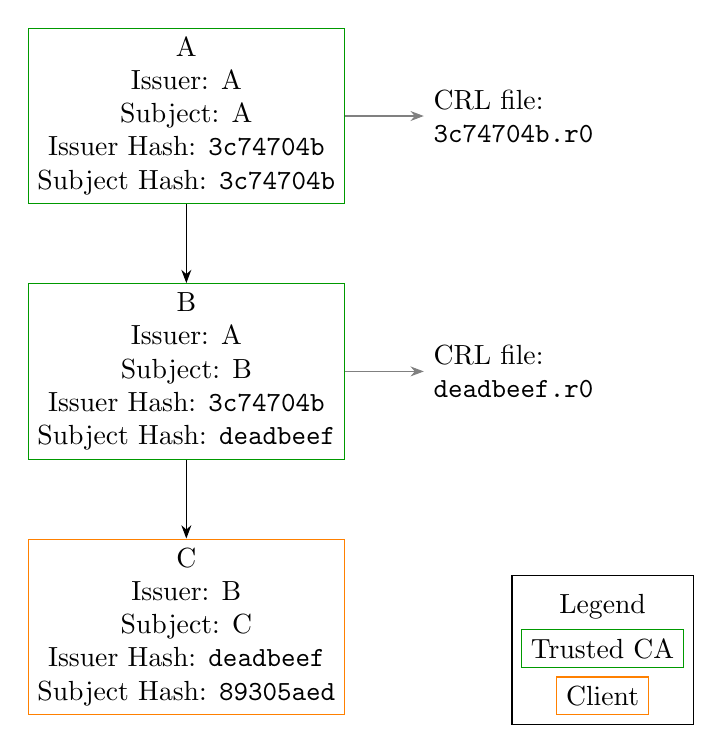
\begin{tikzpicture}
	% Styles.
	[ca/.style={rectangle,draw=green!60!black,minimum height=1cm,minimum width=1.5cm},
	leaf/.style={rectangle,draw=orange,minimum height=1cm, minimum width=1.5cm}]
	% Certificates.
	\node (A) at (0, 0) [ca,align=center] {A \\ Issuer: A \\ Subject: A \\ Issuer Hash: \texttt{3c74704b} \\ Subject Hash: \texttt{3c74704b}};
	\node (B) [below=of A] [ca,align=center] {B \\ Issuer: A \\ Subject: B \\ Issuer Hash: \texttt{3c74704b} \\ Subject Hash: \texttt{deadbeef}};
	\node (C) [below=of B] [leaf,align=center] {C \\ Issuer: B \\ Subject: C \\ Issuer Hash: \texttt{deadbeef} \\ Subject Hash: \texttt{89305aed}};
	\draw[-Stealth] (A) -- (B);
	\draw[-Stealth] (B) -- (C);
	\node (A CRL) [right=of A,align=left] {CRL file: \\ \texttt{3c74704b.r0}};
	\node (B CRL) [right=of B,align=left] {CRL file: \\ \texttt{deadbeef.r0}};
	\draw[-Stealth,gray] (A) -- (A CRL);
	\draw[-Stealth,gray] (B) -- (B CRL);
	% Legend.
	\node (lanchor) at (current bounding box.south east) {};
	\node (legend) at (lanchor) [above=1.1cm] {Legend};
	\node (l1) at (lanchor) [above=0.6cm,draw=green!60!black] {Trusted CA};
	\node (l2) at (lanchor) [above=0.0cm,draw=orange] {Client};
	\node [rectangle,draw,fit=(legend) (l1) (l2)] {};
\end{tikzpicture}
}
\end{makeimage}
\caption{Each CA requires its own CRL file.  The CRL file name is based on the hash of its issuer name.  Note that the \emph{issuer} of the CRL file is the \emph{subject} of its respective CA.}
\end{figure}
\end{center}

One more caveat: OpenSSL does not seem to report any error if the CRL path directory does not exist.  Figures.


% Syncing the Gentoo repository.
\section{2017-08-23 Securely Syncing the Gentoo Repository via a Local Server}

\begin{center}
\begin{figure}
\begin{makeimage}
\fbox{
\begin{tabular}{l|l}
Before: & After: \\
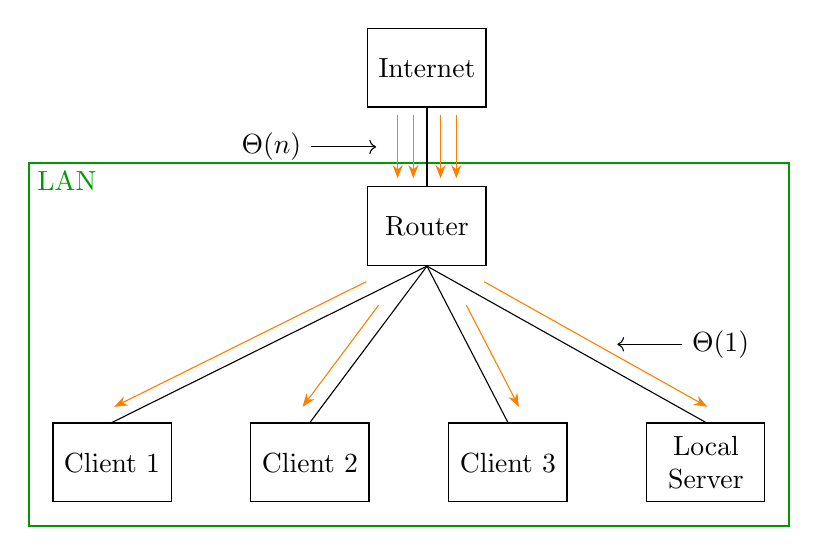
\begin{tikzpicture}
	% Machines.
	[puter/.style={rectangle,draw,minimum height=1cm,minimum width=1.5cm}]
	\node (client1)  at (0, 0) [puter] {Client 1};
	\node (client2)  [right=of client1] [puter] {Client 2};
	\node (client3)  [right=of client2] [puter] {Client 3};
	\node (server)   [right=of client3] [puter] {\parbox{1cm}{\centering Local \\ Server}};
	\node (router)   at (4, 3) [puter] {Router};
	\node (internet) [above=of router] [puter] {Internet};
	% Links.
	\draw (client1.north) -- (router.south)
		node[pos=0.1,left=0.2,circle](c1-r){}
		node[pos=0.9,left=0.2,circle](r-c1){};
	\draw (client2.north) -- (router.south)
		node[pos=0.1,left=0.07,circle](c2-r){}
		node[pos=0.75,left=0.07,circle](r-c2){};
	\draw (client3.north) -- (router.south)
		node[pos=0.1,right=0.07,circle](c3-r){}
		node[pos=0.75,right=0.07,circle](r-c3){};
	\draw (server.north) -- (router.south)
		node[pos=0.1,right=0.2,circle](s-r){}
		node[pos=0.9,right=0.2,circle](r-s){}
		node[pos=0.5,right=0.3,circle](smid){};
	\draw (router.north) -- (internet.south)
		node[pos=0.1,left=0.2,circle](r1-i1){}
		node[pos=0.1,left=0,circle](r2-i2){}
		node[pos=0.1,right=0,circle](r3-i3){}
		node[pos=0.1,right=0.2,circle](r4-i4){}
		node[pos=0.9,left=0.2,circle](i1-r1){}
		node[pos=0.9,left=0,circle](i2-r2){}
		node[pos=0.9,right=0,circle](i3-r3){}
		node[pos=0.9,right=0.2,circle](i4-r4){}
		node[pos=0.5,left=0.3,circle](mid){};
	% Traffic.
	\draw[orange,-Stealth] (r-c1.center) -- (c1-r.center);
	\draw[orange,-Stealth] (r-c2.center) -- (c2-r.center);
	\draw[orange,-Stealth] (r-c3.center) -- (c3-r.center);
	\draw[orange,-Stealth] (r-s.center) -- (s-r.center);
	\draw[orange,-Stealth] (i1-r1.center) -- (r1-i1.center);
	\draw[orange,-Stealth] (i2-r2.center) -- (r2-i2.center);
	\draw[orange,-Stealth] (i3-r3.center) -- (r3-i3.center);
	\draw[orange,-Stealth] (i4-r4.center) -- (r4-i4.center);
	\draw [<-] (mid) -- +(-1, 0) node[left]{$\Theta(n)$};
	\draw [<-] (smid) -- +(1, 0) node[right]{$\Theta(1)$};
	% LAN box.
	\begin{scope}[on background layer]
		\node (bback) [rectangle,thick,draw=green!60!black,inner sep=0.3cm,fit=(client1) (server) (router)] {};
		\node [below right,text=green!60!black] at (bback.north west) {LAN};
	\end{scope}
\end{tikzpicture}
&  % Copy+paste'd
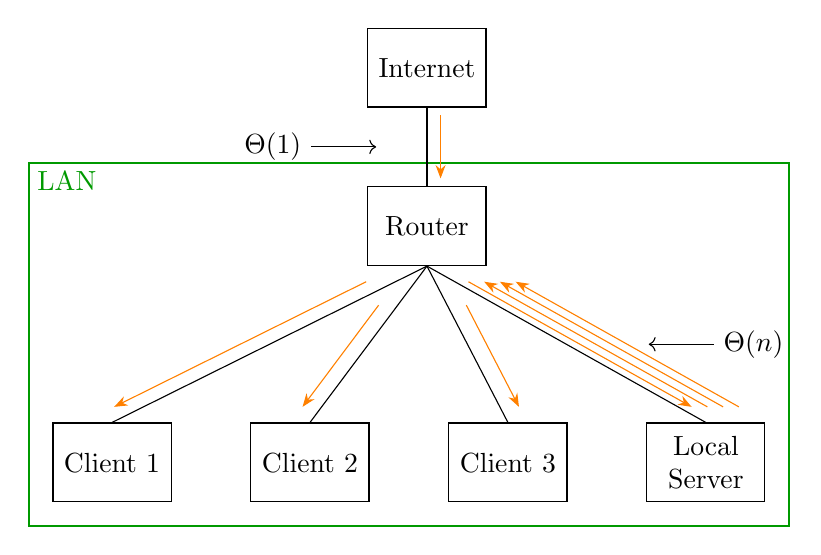
\begin{tikzpicture}
	% Machines.
	[puter/.style={rectangle,draw,minimum height=1cm,minimum width=1.5cm}]
	\node (client1)  at (0, 0) [puter] {Client 1};
	\node (client2)  [right=of client1] [puter] {Client 2};
	\node (client3)  [right=of client2] [puter] {Client 3};
	\node (server)   [right=of client3] [puter] {\parbox{1cm}{\centering Local \\ Server}};
	\node (router)   at (4, 3) [puter] {Router};
	\node (internet) [above=of router] [puter] {Internet};
	% Links.
	\draw (client1.north) -- (router.south)
		node[pos=0.1,left=0.2,circle](c1-r){}
		node[pos=0.9,left=0.2,circle](r-c1){};
	\draw (client2.north) -- (router.south)
		node[pos=0.1,left=0.07,circle](c2-r){}
		node[pos=0.75,left=0.07,circle](r-c2){};
	\draw (client3.north) -- (router.south)
		node[pos=0.1,right=0.07,circle](c3-r){}
		node[pos=0.75,right=0.07,circle](r-c3){};
	\draw (server.north) -- (router.south)
		node[pos=0.1,right=0,circle](s-r){}
		node[pos=0.9,right=0,circle](r-s){}

		node[pos=0.1,right=0.2,circle](s-c1){}
		node[pos=0.9,right=0.2,circle](c1-s){}
		node[pos=0.1,right=0.4,circle](s-c2){}
		node[pos=0.9,right=0.4,circle](c2-s){}
		node[pos=0.1,right=0.6,circle](s-c3){}
		node[pos=0.9,right=0.6,circle](c3-s){}

		node[pos=0.5,right=0.7,circle](smid){};
	\draw (router.north) -- (internet.south)
		node[pos=0.9,right=0,circle](i-s){}
		node[pos=0.1,right=0,circle](s-i){}
		node[pos=0.5,left=0.3,circle](mid){};
	% Traffic.
	\draw[orange,-Stealth] (r-c1.center) -- (c1-r.center);
	\draw[orange,-Stealth] (r-c2.center) -- (c2-r.center);
	\draw[orange,-Stealth] (r-c3.center) -- (c3-r.center);
	\draw[orange,-Stealth] (r-s.center) -- (s-r.center);
	\draw[orange,-Stealth] (s-c1.center) -- (c1-s.center);
	\draw[orange,-Stealth] (s-c2.center) -- (c2-s.center);
	\draw[orange,-Stealth] (s-c3.center) -- (c3-s.center);
	\draw[orange,-Stealth] (i-s.center) -- (s-i.center);
	\draw [<-] (mid) -- +(-1, 0) node[left]{$\Theta(1)$};
	\draw [<-] (smid) -- +(1, 0) node[right]{$\Theta(n)$};
	% LAN box.
	\begin{scope}[on background layer]
		\node (bback) [rectangle,thick,draw=green!60!black,inner sep=0.3cm,fit=(client1) (server) (router)] {};
		\node [below right,text=green!60!black] at (bback.north west) {LAN};
	\end{scope}
\end{tikzpicture}
\end{tabular}
}
\end{makeimage}
\caption{Using a local server for the Gentoo repository takes pressure off of the (often relatively slow) Internet connection and places it onto the (often relatively fast) LAN, especially important for those whose Internet is metered.}
\end{figure}
\end{center}

Running\label{2017-08-23-securely-syncing-the-gentoo-repository-via-a-local-server} multiple Gentoo machines normally means keeping a copy of the Gentoo repository on each machine; by default this also means updating each copy of the repository by having each machine call out to the Gentoo mirrors on a regular basis for updates.  This is a waste of both local and upstream bandwidth and resources, because, within a given time period, the repository is the exact same regardless of the type of machine it is on; instead, it is more efficient to set up one machine as a server that synchronizes with upstream, then have the other local machines synchronize to said local server.  This guide will explain how to do that securely.

Though there are multiple protocols that Portage can use for synchronization, this guide will cover only SSH, and \texttt{rsync+stunnel}.  Both of these are secure, allowing synchronization over an untrusted network, albeit the local server must be trusted.  Securely syncing the server to the upstream repository with \texttt{FEATURES=webrsync-gpg} is not covered here, as it is instead covered \htmladdnormallink{here}{https://wiki.gentoo.org/wiki/Handbook:AMD64/Working/Features#Validated_Gentoo_repository_snapshots}.

\subsection{SSH Synchronization}
One of the pros of SSH-based synchronization is that it requires no extra server configuration for machines that already have SSH access to the server.  The downside is that SSH access means shell access, which might not be desirable if any of the local machines is not fully trusted, for example, because it is running proprietary applications for, say, video games; one could try and circumvent this potential security weakness by giving the SSH user a restricted shell such as \texttt{rssh}, but I was unable to get \texttt{rssh} working with the \texttt{rsync} arguments that Portage wanted to use (note: Portage calls \texttt{rsync} over the SSH session).  Thus I prefer \texttt{rsync+stunnel}, but am including the SSH method for completeness and possible future reference.
\subsubsection{Server} Assuming that \texttt{sshd} is already set up (find one of many guides if it is not), the only thing that may need to be done is to add a special user for synchronization.  In order to add the user, run
\begin{quote}
\begin{verbatim}
	# useradd -m -s /bin/bash rsyncuser
	# passwd rsyncuser
\end{verbatim}
\end{quote}
\ldots then edit the SSH daemon configuration file, usually \texttt{/etc/ssh/sshd_config}, to contain the following line:
\begin{quote}
\begin{verbatim}
	AllowUsers rsyncuser
\end{verbatim}
\end{quote}
Depending on the selected authentication method for SSH, this may be enough to give the user access; however, in the case that only key-based authentication is allowed (usually via something like \texttt{PasswordAuthentication no} \& \texttt{ChallengeResponseAuthentication no} in \texttt{sshd_config}) an SSH keypair will need to be generated for the user and the private key copied to each client that wishes to synchronize with the server.  This can be done with the following commands:
\begin{quote}
\begin{verbatim}
	# cd /home/rsyncuser
	# su rsyncuser
	$ umask 0066
	$ mkdir -p .ssh
	$ ssh-keygen -a 16 -t ed25519
	$ cp .ssh/id_ed25519.pub .ssh/authorized_keys
\end{verbatim}
\end{quote}
This will create a keypair for the \texttt{rsyncyser} and authorize that keypair for SSH login.  The \texttt{.ssh/id_ed25519} file (the private key) will then need to be copied to the client machines, probably via a USB storage device:
\begin{quote}
\begin{verbatim}
	# cp .ssh/id_ed25519 /path/to/probably/usb/storage/device
\end{verbatim}
\end{quote}

This ends the server-side configuration.

\subsubsection{Clients}
By default, Portage knows how to use SSH for synchronization, so basic setup is quite simple, although some of the details are rather esoteric.

In order to tell Portage to synchronize over SSH, if it hasn't been done already, set up the main repository configuration via:
\begin{quote}
\begin{verbatim}
	# mkdir -p /etc/portage/repos.conf
	# cp /usr/share/portage/config/repos.conf /etc/portage/repos.conf/gentoo.conf
\end{verbatim}
\end{quote}
This creates, at the time of this writing, at least, a sane configuration file for the default repository that can then be reconfigured.  With this file created, Portage should function as it always has; the defaults must be overridden in order to actually change its behavior. In order to use SSH, edit the \texttt{/etc/portage/repos.conf/gentoo.conf} file by changing the \texttt{sync-uri} option under the \texttt{[gentoo]} section to read:
\begin{quote}
\begin{verbatim}
	sync-uri = ssh://rsyncuser@192.168.1.1/usr/portage
\end{verbatim}
\end{quote}
\ldots where \texttt{192.168.1.1} is replaced with the network address of the local server.  Portage will now begin trying to sync via SSH.

"Trying" may be the modus operandi depending on whether or not the local server strictly requires keys or will accept user passwords; it is thus useful to understand where Portage stores its SSH information, as its home directory is not \texttt{/home/portage}, but, as \texttt{/etc/passwd} reveals, \texttt{/var/tmp/portage}, thus SSH configuration goes into \texttt{/var/tmp/portage/.ssh}.  In order to get Portage to use \texttt{rsyncuser}'s key, run the following:
\begin{quote}
\begin{verbatim}
	# mkdir -p /var/tmp/portage/.ssh
	# umask 0066
	# cp /path/from/probably/usb/device/with/rsyncusers/key/id_ed25519 /var/tmp/portage/.ssh/id_ed25519
	# chown -R portage:portage /var/tmp/portage/.ssh
\end{verbatim}
\end{quote}
Portage should now pickup \texttt{rsyncuser}'s key when it tries to synchronize.

Admittedly, storing valuable authentication information in a \texttt{/var/tmp} subdirectory seems risky at best.  Another option for storing the key is to place the key at a more stable location and then tell Portage where to find it.  Start by placing the key somewhere safer:
\begin{quote}
\begin{verbatim}
	# mkdir -p /usr/local/portage/.ssh
	# chmod 700 /usr/local/portage/.ssh
	# chown -R portage:portage /usr/local/portage/.ssh
	# mv /var/tmp/portage/.ssh/id_ed25519 /usr/local/portage/.ssh/
\end{verbatim}
\end{quote}
\ldots then tell Portage where to find the key by adding the following line to \texttt{/etc/portage/make.conf}:
\begin{quote}
\begin{verbatim}
	PORTAGE_SSH_OPTS="-i /usr/local/portage/.ssh/id_ed25519"
\end{verbatim}
\end{quote}
Portage will now look for the \texttt{rsyncuser}'s key at the previously-specified location.

This solves the \texttt{rsyncuser}'s key problem, but what about the important \texttt{known_hosts} file?  Well, I didn't get that far.  I don't fully trust of all my machines, and do not want to give all of them shell access to my server, and, since I couldn't get \texttt{rssh} to work with Portage and was looking for an excuse to play with \texttt{stunnel}, I decided to work on it instead, thus \texttt{rsync+stunnel} is the topic of the next section.

\subsection{Rsync+stunnel Synchronization}
This method works by using an \texttt{rsync} daemon to synchronize between the local server and client; however, because \texttt{rsync} is unencrypted, the connection is wrapped via the \texttt{stunnel} daemon, which uses \htmladdnormallink{TLS}{https://en.wikipedia.org/wiki/Transport_Layer_Security} for encryption and authentication.  \texttt{stunnel} must be configured on both the local server and each client.

\subsubsection{Server}
Start by setting up the \texttt{rsync} daemon without \texttt{stunnel}.  By default, Gentoo comes with a disabled but sane configuration file at \texttt{/etc/rsyncd.conf}.  Adding a few extra lines gives, excluding comments, the following:
\begin{quote}
\begin{verbatim}
	pid file = /run/rsyncd.pid
	use chroot = yes
	read only = yes
	hosts allow = 192.168.1.1/16
	reverse lookup = no
	timeout = 60

	[gentoo-portage]
	path = /usr/portage
	comment = Gentoo Portage tree
	exclude = /distfiles /packages
\end{verbatim}
\end{quote}
By default this configuration file creates an \texttt{rsync} \textit{module} that clients can synchronize with; this module is read-only and excludes directories that are not a part of the repository.  The extra options are: \texttt{hosts allow = 192.168.1.1/16}, which tells \texttt{rsync} to only accept connections from hosts in the specified block and must be appropriate to the local network; \texttt{reverse lookup = no}, which disables reverse-DNS lookups of client IP addresses; and \texttt{timeout = 60}, which sets a small timeout for unresponsive clients.  See \texttt{man 5 rsyncd.conf} for details; the extra options are not strictly necessary for the purposes of this guide.

The next step is to install and configure \texttt{stunnel}.  This involves four steps: installing the program, configuring the service, generating certificates, and creating the service: To install \texttt{stunnel}, run:
\begin{quote}
\begin{verbatim}
	# emerge -av stunnel
\end{verbatim}
\end{quote}
For convenience, the Gentoo developers created a useful example configuration file for \texttt{rsync+stunnel} which may be installed by running:
\begin{quote}
\begin{verbatim}
	USE="stunnel" emerge -av rsync
\end{verbatim}
\end{quote}
This creates the file \texttt{/etc/stunnel/rsyncd.conf}.  Move it to \texttt{/etc/stunnel/rsyncd-stunnel.conf} for \texttt{init} scripts (later), and reconfigure it such that, excluding comments, it has the following options:
\begin{quote}
\begin{verbatim}
	foreground = no
	pid = /var/run/stunnel/rsyncd-stunnel.pid
	socket = l:TCP_NODELAY=1
	socket = r:TCP_NODELAY=1
	setuid = root
	setgid = root

	[rsync]
	accept = 874
	cert = /etc/stunnel/rsyncd-stunnel.crt
	key  = /etc/stunnel/rsyncd-stunnel.key
	client = no

	exec = /usr/bin/rsync
	execargs = rsync --server --daemon --config=/etc/rsyncd.conf .
\end{verbatim}
\end{quote}
Most of these options come with the default configuration file, but make sure to change the \texttt{pid} option.  The \texttt{cert} and \texttt{key} options specify where the \htmladdnormallink{X.509}{https://en.wikipedia.org/wiki/X.509} certificate and its key are to be loaded from (they will be generated later).  Port \texttt{874} is used in place of \texttt{873}, as it is not a plaintext \texttt{rsync} service.  Client verification is not wanted here, so make sure to remove any \texttt{verify} and \texttt{CAfile} lines.

In order to generate the server's certificate, run the following series of commands:
\begin{quote}
\begin{verbatim}
	# cd /etc/stunnel
	# umask 0077
	# openssl genrsa -out rsyncd-stunnel.key 4096
	# openssl req -key rsyncd-stunnel.key -new -x509 -days 7200 -sha512 -out rsyncd-stunnel.crt -subj '/CN=rsyncd-stunnel/'
\end{verbatim}
\end{quote}
The short story here is that this will create a certificate and key pair for TLS that will last for almost 20 years, see \texttt{man genrsa} and \texttt{man req} for details.

Finally, create the service with:
\begin{quote}
\begin{verbatim}
	# cd /etc/init.d
	# ln -s stunnel rsyncd-stunnel
\end{verbatim}
\end{quote}
This uses the default \texttt{stunnel} init script, except it will look for a configuration file at \texttt{/etc/stunnel/rsyncd-stunnel.conf}, hence the earlier renaming that was done.  To start the service, run \texttt{rc-service rsyncd-stunnel start}, and don't forget to add it to the default runlevel via:
\begin{quote}
\begin{verbatim}
	# rc-update add rsyncd-stunnel default
\end{verbatim}
\end{quote}

The server should now be configured and ready for synchronization.  The clients must now be configured to trust and use the server.

\subsubsection{Clients}
The client must now be configured so that when Portage attempts to sync it will use the secure connection \textbf{and} it will validate that it is syncing with the server, otherwise a malicious actor could imitate the server and send a compromised repository.  This involves installing and configuring \texttt{stunnel}, configuring Portage, then creating the service.

Begin by installing \texttt{stunnel}:
\begin{quote}
\begin{verbatim}
	# emerge -av stunnel
\end{verbatim}
\end{quote}
\ldots then configure \texttt{stunnel} so that, without comments, the configuration file \texttt{/etc/stunnel/stunnel.conf} reads:
\begin{quote}
\begin{verbatim}
	setuid = stunnel
	setgid = stunnel
	pid = /run/stunnel/stunnel.pid
	socket = l:TCP_NODELAY=1
	socket = r:TCP_NODELAY=1

	[rsync-stunnel]
	client     = yes
	CAfile     = /etc/stunnel/rsyncd-stunnel.crt
	verifyPeer = yes
	accept     = 127.0.0.1:873
	connect    = 192.168.1.200:874
\end{verbatim}
\end{quote}
This creates an \texttt{stunnel} \emph{service}.  The \texttt{client} argument lets \texttt{stunnel} know to run \texttt{rsync} as a client rather than as a server.  The \texttt{CAfile} argument specifies the location of the server certificate to use (note that it has not yet been copied over to the client).  The \texttt{verifyPeer} is especially important as enabling it will actually validate the server certificate; without this enabled a malicious actor could intercept and modify the traffic.  The \texttt{accept} argument specifies where the \texttt{stunnel} program will listen for client connections, Portage will later be configured to make connections here.  The \texttt{connect} argument specifies where the \texttt{stunnel} program will connect to; it must be set to the address and port of the local server.  The other options are fairly standard.  Note that, unlike the server, this setup is using the default \texttt{stunnel} settings, configuring multiple \texttt{stunnel} services at the OpenRC level would require modifying a few parameters, such as the PID (Process ID) and the filename of the configuration.

Now that \texttt{stunnel} has been configured, make sure to copy the certificate from the local server to the client.  This should be done via a trusted storage device (USB stick, SD Card, \&c.) or the certificate retrieved via a command such as OpenSSL's \texttt{s\_client} (usage not covered here) and its fingerprint manually verified.
\begin{quote}
\begin{verbatim}
	# cp /path/from/secure/storage/device /etc/stunnel/rsyncd-stunnel.crt
\end{verbatim}
\end{quote}
\texttt{stunnel} now has all that it needs to securely tunnel a connection to the server.

Portage must now be configured to use the secure tunnel.  As with SSH configuration, begin by overriding the default repository configuration:
\begin{quote}
\begin{verbatim}
	# mkdir -p /etc/portage/repos.conf
	# cp /usr/share/portage/config/repos.conf /etc/portage/repos.conf/gentoo.conf
\end{verbatim}
\end{quote}
\ldots then modify the \texttt{sync-uri} argument to correspond to the \texttt{accept} argument configured in \texttt{stunnel}:
\begin{quote}
\begin{verbatim}
	sync-uri = rsync://127.0.0.1:873/gentoo-portage
\end{verbatim}
\end{quote}
This will synchronize with the \texttt{gentoo-portage} module defined on the local server's \texttt{/etc/rsyncd.conf}.  Note how the use of \texttt{stunnel} is completely transparent to Portage.  This has the minor disadvantage that error diagnostics must be found in log message from \texttt{stunnel} and not the Portage frontend, but is usually not a problem once things have been configured properly.

Next, start the service and add it to the default runlevel:
\begin{quote}
\begin{verbatim}
	# rc-service stunnel start
	# rc-update add stunnel default
\end{verbatim}
\end{quote}
\ldots then try it out with:
\begin{quote}
\begin{verbatim}
	# emerge --sync
\end{verbatim}
\end{quote}
Portage should now be securely synchronizing to the local server!  Repeat these steps for each client that needs to synchronize with the local server.


% Ancient Apparition Bowling
\section{2017-07-17 Ancient Apparition Bowling}
This is a silly metagame that I came up with for a DotA2 custom game.  It may not be possible to beat, but I've yet to try all strategies.

\subsection*{Origin}
Mercilessly slaughtering bots using weird combinations of cheats in DotA2 is an easy way to blow off a little steam after a difficult match.  One day I decided to go "bowling" with Ancient Apparition; I'd cheat to maximum level, 6-slot, enable wtf mode, and snipe the bots from base with his ultimate.
This is loads of fun, until the creeps start pushing towers, at which point the bots also take advantage of wtf mode and begin spamming fortify, leading to a frustrating stalemate.  The workaround for this is to disable wtfmode and instead use the \texttt{-refresh} cheat, which, although it does reset fortify cooldowns, can be used in conjunction with a Refresher Orb to blast the bots with two ultimates while giving them only one fortify.

The result is a semi-functional slaughtering of bots, although having to constantly open the command prompt to paste and submit the \texttt{-refresh} command gets annoying after a while; sadly, there doesn't seem to be a way to disable the bots' fortify spam.  After a little bit of this, I noticed that the cooldown of the metaphorical bowling ball and the travel time were not that far apart, leading me to wonder if I could play this game successfully without having to spam cheat commands (and reset the fortify cooldown) all game long.  Thus "Ancient Apparition Bowling" was born.

\subsection*{Rules}
These are the rules of the game, and though they may not be comprehensive, you should be able to understand the jist of them.  First, stay in fountain for the duration of the match.  Second, use cheats to give yourself max level (\texttt{-lvlup 25}), 6-slots (\texttt{-item <name>}), and vision (\texttt{-allvision}).  Third, no backpack, stash, or other item-use shenanegains; stick to your 6 slots.  Fourth, no bots on your team and five bots of highest difficulty on the other team.  That's it!
\begin{figure}
\includegraphics[scale=0.33]{files/blog/2017_07_17_ancient_apparition_bowling/fountain.png}
\caption{Where you will be spending all of your time.}
\end{figure}

Your goal is now to destroy the bots' ancient before the bots level up enough to tank through your ult and push your base.  This is more difficult than it sounds, as the bots are actually rather crafty and level up sooner than you might expect.

\subsection*{Strategy}
My current build involves getting an Aghaim's Scepter, Octarine Core, Refresher Orb, and 3 Aether Lens.  Perhaps you can think up something better.
\begin{figure}
\includegraphics{files/blog/2017_07_17_ancient_apparition_bowling/items.png}
\end{figure}

It is difficult to push all lanes at once, since the bots can quickly respawn at lower levels, and you only have so many ultimates to shoot off.  It would thus seem prudent to choose a particular lane to hammer, but how to do so isn't actually obvious.

The strategy that I tried was to focus the enemy creeps at their spawning point in a side lane.  This can be done by firing consistently at the 18 and 48 second marks towards the front of their 3rd tower. This will obliterate all of the creeps during the early part of the game.  Make sure to adjust your ultimate slightly to the left each time in order to adjust for the micro-delay between your ult going off cooldown and actually launching your ult; you can reset this after a while with a Refresher Orb.
\begin{figure}
\includegraphics[scale=0.33]{files/blog/2017_07_17_ancient_apparition_bowling/towerhit.png}
\caption{Killing creeps as soon as they spawn.}
\end{figure}

Though this may at first seem like a good way to get the creeps to push the tower, the bots are actually crafty enough to pull the creeps behind the tower, limiting the amount of damage done.  While I was able to eventually push to their barracks, at this point the other bots also helped pull the creeps behind the barracks, and eventually became strong enough to tank the ult and push my base, thus making this a losing strategy.
\begin{figure}
\includegraphics[scale=0.33]{files/blog/2017_07_17_ancient_apparition_bowling/botpull.png}
\caption{Sneaky bots pulling creeps away from the tower.}
\end{figure}

A possible variation would be to try focusing down the bots themselves, but this is tricky as they often move out of the ult's way.  A hybrid combination may involve finding a position where the bots and creeps are likely to align, then aiming to kill the creeps and probably the bots.  It may also be easier to push straight up middle rather than taking out a side lane first, especially as the bots seem found of charging up mid.

I've yet to win at this metagame.  It might not even be plausible.  Try it yourself and see what happens!

\subsection*{Addendum}
Between inventing this game, writing this article, and getting the screenshots, the bot fortify spam in wtf mode seems to have stopped.

\end{document}
